\documentclass[a4paper,12pt,openany]{book}
\usepackage{graphicx}
\usepackage[export]{adjustbox}
\usepackage{subcaption}
\graphicspath{{Pics/}}
\usepackage{charter}
\usepackage{fancyhdr}
\usepackage{enumerate}
\usepackage{enumitem}
\usepackage{siunitx}
\usepackage{amssymb}
\usepackage{longtable}
\usepackage{multicol}
\usepackage{multirow}
\usepackage{hhline}
\usepackage{parskip}
\setlength{\parskip}{6pt}
\usepackage{ragged2e}
\usepackage{geometry} %margin
\geometry{left=2.1cm,right=2.1cm,top=3cm,bottom=3cm}
\usepackage{setspace}
\SetSinglespace{1.2}
\singlespacing
\renewcommand{\ttfamily}{\fontfamily{pcr}\selectfont}
%\renewcommand{\familydefault}{\rmdefault}

\usepackage[,table]{xcolor}
\definecolor{LightBlue}{cmyk}{0.16,0.03,0.04,0}
\definecolor{Title}{cmyk}{0.8,0.1,0,0.3}
\setlength{\arrayrulewidth}{0.3mm}
\setlength{\tabcolsep}{2pt}
\setlength{\headheight}{15pt}
\renewcommand{\arraystretch}{1}
\usepackage{tikz}
\usepackage{nicematrix}
\newcommand*\circled[1]{\tikz[baseline=(char.base)]{\node[shape=circle,draw,inner sep=1pt] (char) {#1};}}

\newcolumntype{s}{>{\columncolor{Title}\RaggedLeft} m{3.5em}} % columntype for chapter title
\newcolumntype{d}{>{\columncolor{LightBlue}\RaggedRight} m{\textwidth}} % columntype for code bloc
\newcolumntype{a}{>{\columncolor{LightBlue}\RaggedRight} m{0.96\textwidth}} % columntype for secondary code bloc

\usepackage{titlesec}
\usepackage[hidelinks]{hyperref}
\urlstyle{same}

\captionsetup[figure]{labelsep=period,font={bf}}
\captionsetup[table]{font={bf},labelsep=period}

\newcommand{\titlename}{}

\newcommand{\chaptertitle}[2]{ %reset chapter format
\vspace{-120pt}
\gdef\titlename{#1}
{
\SetSinglespace{1.1}
\singlespacing
\Huge\bfseries
\setlength{\tabcolsep}{8pt}
\renewcommand{\arraystretch}{1.5}
\begin{tabular}{s >{\RaggedRight}m{14.5em}}
\textcolor{white}{Chapter\newline\thechapter}&\textcolor{Title}{#2}
\end{tabular}
}
}

\newcommand{\partpic}[1]{%insert picture
    \tikz[remember picture,overlay] \node at (current page.center){\includegraphics[width=\paperwidth]{#1}};
}

\titleformat{\part} %reset part %format
{\huge\bfseries} % format
{} % label
{0em} % sep
{\Centering} % before-code

\titleformat{\chapter} %reset chapter %format
{\huge\bfseries} % format
{} % label
{0em} % sep
{\Centering} % before-code
\titlespacing{\chapter}{0pt}{0pt}{0pt}

\titleformat{\section} %reset section %format
{\Large\bfseries} % format
{\textcolor{Title}{\thesection}} % label
{0.5em} % sep
{\color{Title}} % before-code
\titlespacing{\section}{0pt}{12pt}{6pt}

\titleformat{\subsection} %reset subsection %format
{\large\bfseries} % format
{\textcolor{Title}{\thesubsection}} % label
{0.5em} % sep
{\color{Title}} % before-code
\titlespacing{\subsection}{0pt}{8pt}{6pt}

\newenvironment{term}[1]{
    \textbf{#1}

    \leftskip 1em
    \parskip 0pt
}

\newenvironment{secterm}[1]{
    \textbf{#1}

    \leftskip 2em
    \parskip 0pt
}

\newenvironment{codebloc}{ %define code bloc style
    \ttfamily\footnotesize
    \renewcommand{\arraystretch}{1}
}

\newcommand{\note}[2][NOTE]{ %Note/Tips
\vspace{6pt}
\begin{tabular}{b{\textwidth}}
\hline
\fontfamily{phv}\selectfont \textbf{#1}\\
\leftskip 1em #2\\
\hline
\end{tabular}
}

\newcommand{\secnote}[2][NOTE]{ %Note/Tips
\vspace{6pt}
\begin{tabular}{b{0.93\textwidth}}
\hline
\fontfamily{phv}\selectfont \textbf{#1}\\
\leftskip 1em #2\\
\hline
\end{tabular}
}

\title{ESP32-C3 Wireless Adventure\par \Large A Comprehensive Guide to IoT}
\author{Espressif Systems}
\date{\today}

\pagestyle{fancy} % reset head&foot
\fancyhead{} % clear all header fields
\renewcommand\headrulewidth{0pt}
\fancyfoot{} % clear all footer fields

\begin{document}

\maketitle

\tableofcontents

\newpage
\begin{center}
    \textcolor{Title}{\large\bfseries Introduction}
\end{center}
ESP32-C3 is a single-core Wi-Fi and Bluetooth 5 (LE) microcontroller SoC, based on the open-source RISC-V architecture. It strikes the right balance of power, I/O capabilities, and security, thus offering the optimal cost-effective solution for connected devices. To show various applications of the ESP32-C3 family, this book by Espressif will take you on an interesting journey through AIoT, starting from the basics of IoT project development and environment setup to practical examples. The first four chapters talk about IoT, ESP RainMaker and ESP-IDF. Chapter 5 and 6 brief on hardware design and driver development. As you progress, you’ll discover how to configure your project through Wi-Fi networks and mobile Apps. Finally, you’ll learn to optimize your project and put it into mass production.

If you are an engineer in related fields, a software architect, a teacher, a student, or anyone who has an interest in IoT, this book is for you.

You may download the code example used in this book from Espressif’s site on GitHub. For latest information on IoT development, please follow our official account.

% Preface
\newpage
\begin{center}
    \textcolor{Title}{\LARGE\bfseries Preface}
\end{center}

\subsection*{An Informatising World}
Riding the wave of Internet, Internet of Things (IoT) made its grand debut to become a new type of infrastructure in digital economy. To bring the technology closer to the public, Espressif Systems works for the vision that developers from all walks of life can use IoT to solve some of the most pressing problems of our times. A world of “Intelligent Network of All Things” is what we are expecting from the future.

Designing our own chips makes a critical component of that vision. It is to be a marathon, requiring constant breakthroughs against technological boundaries. From the “Game Changer” ESP8266 to the ESP32 series integrating Wi-Fi and Bluetooth$^\circledR$ (LE) connectivity, followed by ESP32-S3 equipped by AI acceleration, Espressif never stops researching and developing products for AIoT solutions. With our open-source software, such as the IoT Development Framework ESP-IDF, Mesh Development Framework ESP-MDF, and Device Connectivity Platform ESP RainMaker, we have created an independent framework for building AIoT applications.

As of July 2022, the cumulative shipments of Espressif’s IoT chipsets have exceeded 800 million, leading in the Wi-Fi MCU market and powering up a huge number of connected devices worldwide. Pursuit for excellence makes every Espressif product a big hit for its high level of integration and cost efficiency. The release of ESP32-C3 marks a significant milestone of Espressif’s self-developed technology. It is a single-core, 32-bit, \textbf{RISC-V-based} MCU with 400KB of SRAM, which can run at 160MHz. It has integrated 2.4 GHz Wi-Fi and Bluetooth 5 (LE) with a long-range support. It strikes a fine balance of power, I/O capabilities, and security, thus offering the optimal cost-effective solution for connected devices. Based on such powerful ESP32-C3, this book is intended to help readers understand IoT-related knowledge with detailed illustration and practical examples.

\subsection*{Why we wrote this book?}
Espressif Systems is more than a semiconductor company. It is also an IoT platform company, which always strives for breakthroughs and innovations in the field of technology. At the same time, Espressif has open-sourced and shared its self-developed operating system and software framework with the community, forming a unique ecosystem. Engineers, makers, and technology enthusiasts actively develop new software applications based on Espressif’s products, freely communicate, and share their experience. You can see developers’ fascinating ideas on various platforms all the time, such as YouTube and GitHub. The popularity of Espressif’s products has stimulated an increasing number of authors who have produced over 100 books based on Espressif chipsets, in more than ten languages, including English, Chinese, German, French, and Japanese.

It is the support and trust of community partners that encourages Espressif's continuous innovation. “We strive to make our chips, operating systems, frameworks, solutions, Cloud, business practices, tools, documentation, writings, ideas, etc., ever more relevant to the answers people need in contemporary life’s most pressing problems. This is Espressif’s highest ambition and moral compass.” said Mr. Teo Swee Ann, Founder and CEO of Espressif.

Espressif values reading and ideas. As the continuous upgrading of IoT technology poses higher requirements on engineers, how can we help more people to quickly master IoT chips, operating systems, software frameworks, application schemes and cloud service products? As the saying goes, it is better to teach a man how to fish than to give him fish. In a brainstorming session, it occurred to us that we could write a book to systematically sort out the key knowledge of IoT development. We hit it off, quickly gathered a group of senior engineers, and combined the experience of the technical team in embedded programming, IoT hardware and software development, all contributing to the publishing of this book. In the process of writing, we tried our best to be objective and fair, stripped of the cocoon, and use concise expressions to tell the complexity and charm of the Internet of Things. We carefully summarised the common questions, referred to the feedback and suggestions of the community, in order to clearly answer the questions encountered in the development process, and provide practical IoT development guidelines for relevant technicians and decision-makers.

\subsection*{Book Structure}
This book takes an engineer-centred perspective and expounds the necessary knowledge for IoT project development step by step. It is composed of four parts, as follows:
\begin{itemize}
    \item \textbf{Preparation} (Chapter 1–4): This part introduces the architecture of IoT, typical IoT project framework, the ESP RainMaker$^\circledR$ cloud platform, and the development environment ESP-IDF, so as to lay a solid foundation for IoT project development.
    \item \textbf{Hardware and Driver Development} (Chapter 5–6): Based on the ESP32-C3 chipset, this part elaborates on the minimum hardware system and driver development, and implements the control of dimming, colour grading, and wireless communication.
    \item \textbf{Wireless Communication and Control} (Chapter 7–11): This part explains the intelligent Wi-Fi configuration scheme based on ESP32-C3 chip, local \& cloud control protocols, and local \& remote control of devices. It also provides schemes for developing smartphone apps, firmware upgrade, and version management.
    \item \textbf{Optimisation and Mass Production} (Chapter 12-15): This part is intended for advanced IoT applications, focusing on optimisation of products in power management, low-power optimisation, and enhanced security. It also introduces firmware burning and testing in mass production, and how to diagnose the running status and logs of device firmware through the remote monitoring platform ESP Insights.
\end{itemize}

\subsection*{About the Source Code}
Readers can run the example programmes in this book, either by entering the code manually or by using the source code that accompanies the book. We emphasise the combination of theory and practice, and thus set a \textit{Practice} section based on the Smart Light project in almost every chapter. All the codes are open-sourced. Readers are welcome to download the source code and discuss it in the sections related to this book on GitHub and our official forum esp32.com. The open-sourced code of this book is subject to the terms of Apache License 2.0.

\subsection*{Author’s Note}
This book is officially produced by Espressif Systems and is written by the company’s senior engineers. It is suitable for managers and R\&D personnel in IoT-related industries, teachers and students of related majors, and enthusiasts in the field of Internet of Things. We hope that this book can serve as a work manual, a reference, and a bedside book, to be like a good tutor and friend.

While compiling this book, we referred to some relevant research results of experts, scholars, and technicians at home and abroad, and we did our best to cite them according to academic norms. However, it is unavoidable that there should be some omissions, so here we would like to express our deep respect and gratitude to all the relevant authors. In addition, we have quoted information from the Internet, so we would like to thank the original authors and publishers and apologise that we cannot indicate the source of every piece of information.

In order to produce a book of high quality, we have organised rounds of internal discussions, and learned from the suggestions and feedback of trial readers and publisher editors. Here, we would like to thank you again for your help which all contributed to this successful work.

Last, but the most importantly, thanks to everyone at Espressif who has worked so hard for the birth and popularization of our products.

The development of IoT projects involves a wide range of knowledge. Limited to the length of the book, as well as the level and experience of the author, omissions are unavoidable. Therefore, we kindly request that experts and readers criticise and correct our mistakes. If you have any suggestions for this book, please contact us at \texttt{book@espressif.com}. We look forward to your feedback.

\newpage
%How to use this book?
\begin{center}
    \textcolor{Title}{\LARGE\bfseries How to use this book?}
\end{center}

\vspace{6pt}
The code of the projects in this book has been open sourced. You can download it from our GitHub repository and share your thoughts and questions on our official forum.

\begin{tabular}{d}
    GitHub: \url{https://github.com/espressif/book-esp32c3-iot-projects}
    
    Forum: \url{https://www.esp32.com/bookc3}
\end{tabular}

Throughout the book, there will be parts highlighted as shown below.

\note[Source code]{In this book, we emphasise the combination of theory and practice, and thus set a \textit{Practice} section about the Smart Light project in almost every chapter. Corresponding steps and source page will be marked between two lines beginning with the tag \textbf{Source code}.}

\vspace{6pt}
\note[NOTE/TIPS]{This is where you may find some critical information and reminding for successfully debugging your programme. They will be marked between two thick lines beginning with the tag \textbf{NOTE} or \textbf{TIPS}.}

Most of the commands in this book are executed under Linux, prompted by the character “\verb|$|”. If the command requires superuser privileges to execute, the prompt will be replaced by “\verb|#|”. The command prompt on Mac systems is “\verb|%|”, as used in Section 4.2.3 Installing ESP-IDF on Mac.

The body text in this book will be printed in Charter, while the code examples, components, functions, variables, code file names, code directories, and strings will be in \texttt{Courier New}.

Commands or texts that need to be input by the user, and commands that can be entered by pressing the “Enter” key will be printed in \textbf{\texttt{Courier New bold}}. Logs and code blocks will be presented in \colorbox{LightBlue}{light blue boxes}.

\vspace{6pt}
\textcolor{Title}{\large\bfseries Example:}

Second, use \texttt{esp-idf/components/nvs\_flash/nvs\_partition\_generator/nvs\_\\
partition\_gen.py} to generate the NVS partition binary file on the development host with the following command:

\begin{tabular}{d}
\footnotesize\texttt{\$ \bfseries python \$IDF\_PATH/components/nvs\_flash/nvs\_partition\_generator/nvs\_partition\_\newline gen.py --input\ mass\_prod.csv --output mass\_prod.bin --size NVS\_PARTITION\_SIZE}
\end{tabular}

{\makeatletter
\let\ps@plain\ps@empty
\makeatother
\part[Preparation]{\setcounter{page}{1}\partpic{Starting/1c}}
}

\fancyfoot[LE]{\fontfamily{cmss}\selectfont{\textbf{\thepage} \ \textit{ESP32-C3 Wireless Adventure: A Comprehensive Guide to IoT}}}
\fancyfoot[RO]{\fontfamily{cmss}\selectfont{\textit{Chapter \thechapter. \titlename} \ \textbf{\thepage}}}

\chapter[Introduction to IoT]{\chaptertitle{Introduction to IoT}{Introduction to IoT}}

\vspace{24pt}
At the end of the 20th century, with the rise of computer networks and communication technologies, Internet rapidly integrated into people's lives. As Internet technology continues to mature, the idea of Internet of Things (IoT) was born. Literally, IoT means an Internet where things are connected. While the original Internet breaks the limits of space and time and narrows the distance between “person and person”, IoT makes “things” an important participant, bringing “people” and “things” closer together. In the foreseeable future, IoT is set to become the driving force of the information industry.

So, what is the Internet of Things?

It is hard to accurately define the Internet of Things, as its meaning and scope are constantly evolving. In 1995, Bill Gates first brought up the idea of IoT in his book \textit{The Road Ahead}. Simply put, IoT enables objects to exchange information with each other through Internet. Its ultimate goal is to establish an “Internet of Everything”. This is an early interpretation of IoT, as well as a fantasy of future technology. Thirty years later, with the rapid development of economy and technology, the fantasy is coming into reality. From smart devices, smart homes, smart cities, Internet of Vehicles and wearable devices, to the “metaverse” supported by IoT technologies, new concepts are constantly emerging. In this chapter, we will begin with an explanation of the architecture of Internet of Things, and then introduce the most common IoT application, the smart home, in order to help you get a clear understanding of IoT.

\section{Architecture of IoT}

Internet of Things involves multiple technologies which have different application needs and forms in different industries. In order to sort out the structure, the key technologies and application characteristics of IoT, it is necessary to establish a unified architecture and a standard technical system. In this book, the architecture of IoT is simply divided into four layers: perception \& control layer, network layer, platform layer, and application layer.

\begin{term}{Perception \& Control Layer}
    As the most basic element of the IoT architecture, perception \& control layer is the core to realise the comprehensive sensing of IoT. Its main function is to collect, identify and control information. It consists of a variety of devices with the ability of perception, identification, control and execution, and is responsible for retrieving and analysing data such as material properties, behavioural trends, and device status. In this way, IoT gets to recognise the real physical world. Besides, the layer is also able to control the status of the device.

    \parskip 6pt
    The most common devices of this layer are various sensors, which play an important role in information collection and identification. Sensors are like human sensory organs, such as photosensitive sensors equalling to vision, acoustic sensors to hearing, gas sensors to smelling, and pressure- and temperature-sensitive sensors to touching. With all these “sensory organs”, objects become “alive” and capable of intelligent perception, recognition and manipulation of the physical world.
\end{term}

\begin{term}{Network Layer}
    The main function of the network layer is to transmit information, including data obtained from the perception \& control layer to specified target, as well as commands issued from the application layer back to the perception \& control layer. It serves as an important communication bridge connecting different layers of an IoT system. To set up a basic model of Inter\textbf{net} of Things, it involves two steps to integrate objects into a \textbf{net}work: access to Internet and transmission through Internet.
    
    \parskip 6pt
    \begin{secterm}{Access to Internet}
        Internet enables interconnection between person and person, but fails to include things into the big family. Before the advent of IoT, most things were not “network-able”. Thanks to the continuous development of technology, IoT manages to connect things to the Internet, thus realizing interconnection between “people and things”, and “things and things”. There are two common ways to implement Internet connection: wired network access and wireless network access.

        \parskip 6pt
        Wired network access methods include Ethernet, serial communication (e.g., RS-232, RS-485) and USB, while wireless network access depends on wireless communication, which can be further divided into short-range wireless communication and long-range wireless communication.
        
        Short-range wireless communication includes ZigBee, Bluetooth$^\circledR$, Wi-Fi, Near-Field Communication (NFC), and Radio Frequency Identification (RFID). Long-range wireless communication includes Enhanced Machine Type Communication (eMTC), LoRa, Narrow Band Internet of Things (NB-IoT), 2G, 3G, 4G, 5G, etc.
    \end{secterm}

    \begin{secterm}{Transmission through Internet}
    Different methods of Internet access lead to corresponding physical transmission link of data. The next thing is to decide which communication protocol to use to transmit the data. Compared with Internet terminals, most IoT terminals currently have fewer available resources, such as processing performance, storage capacity, network rate, etc., so it is necessary to choose a communication protocol that occupies fewer resources in IoT applications. There are two communication protocols that are widely used today: Message Queuing Telemetry Transport (MQTT) and Constrained Application Protocol (CoAP).
    \end{secterm}
\end{term}

\begin{term}{Platform Layer}
    The platform layer mainly refers to IoT cloud platforms. When all IoT terminals are networked, their data need to be aggregated on an IoT cloud platform to be calculated and stored. The platform layer mainly supports IoT applications in facilitating access and management of massive devices. It connects IoT terminals to the cloud platform, collects terminal data, and issues commands to terminals, so as to implement remote control. As an intermediate service to assign equipment to industry applications, the platform layer plays a connecting role in the entire IoT architecture, carrying abstract business logic and standardized core data model, which can not only realize rapid access of devices, but also provide powerful modular capabilities to meet various needs in industry application scenarios. The platform layer mainly includes functional modules such as device access, device management, security management, message communication, monitoring operation and maintenance, and data applications.

    \parskip 6pt
    \begin{itemize}
        \item Device access, realising the connection and communication between terminals and IoT cloud platforms.
        \parskip 0pt
        \item Device management, including functions such as device creation, device maintenance, data conversion, data synchronization, and device distribution.
        \item Security management, ensuring the security of IoT data transmission from the perspectives of security authentication and communication security.
        \item Message communication, including three transmission directions, that is, the terminal sends data to the IoT cloud platform, the IoT cloud platform sends data to the server side or other IoT cloud platforms, and the server side remotely controls IoT devices.
        \item Monitoring O\&M, involving monitoring and diagnosis, firmware upgrade, online debugging, log services, etc.
        \item Data applications, involving the storage, analysis and application of data.
    \end{itemize}
\end{term}

\begin{term}{Application Layer}
    The application layer uses the data from the platform layer to manage the application, filtering and processing them with tools such as databases and analysis software. The resulting data can be used for real-world IoT applications such as smart healthcare, smart agriculture, smart homes, and smart cities.
\end{term}

Of course, the architecture of IoT can be subdivided into more layers, but no matter how many layers it consists of, the underlying principle remains essentially the same. Learning about the architecture of IoT helps deepen our understanding of IoT technologies and build fully functional IoT projects.

\section{IoT Application in Smart Homes}
IoT has penetrated into all walks of life, and the most closely related IoT application to us is the smart home. Many traditional appliances are now equipped with one or more IoT devices, and many newly built houses are designed with IoT technologies from the start. Figure 1.1 shows some common smart home devices.

\begin{figure}[!ht]
    \centering
    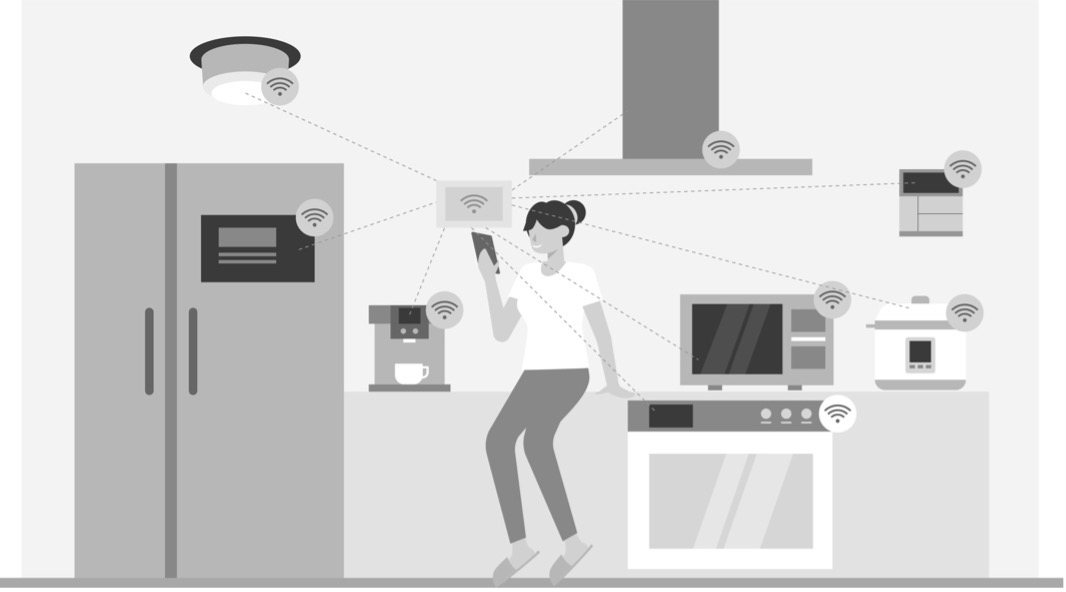
\includegraphics[width=0.75\textwidth]{D1Z/1-1}
    \caption{Common smart home devices}
\end{figure}

The development of smart home can be simply divided into smart product stage, scene interconnection stage and intelligent stage, as shown in Figure 1.2.

\begin{figure}[!ht]
    \centering
    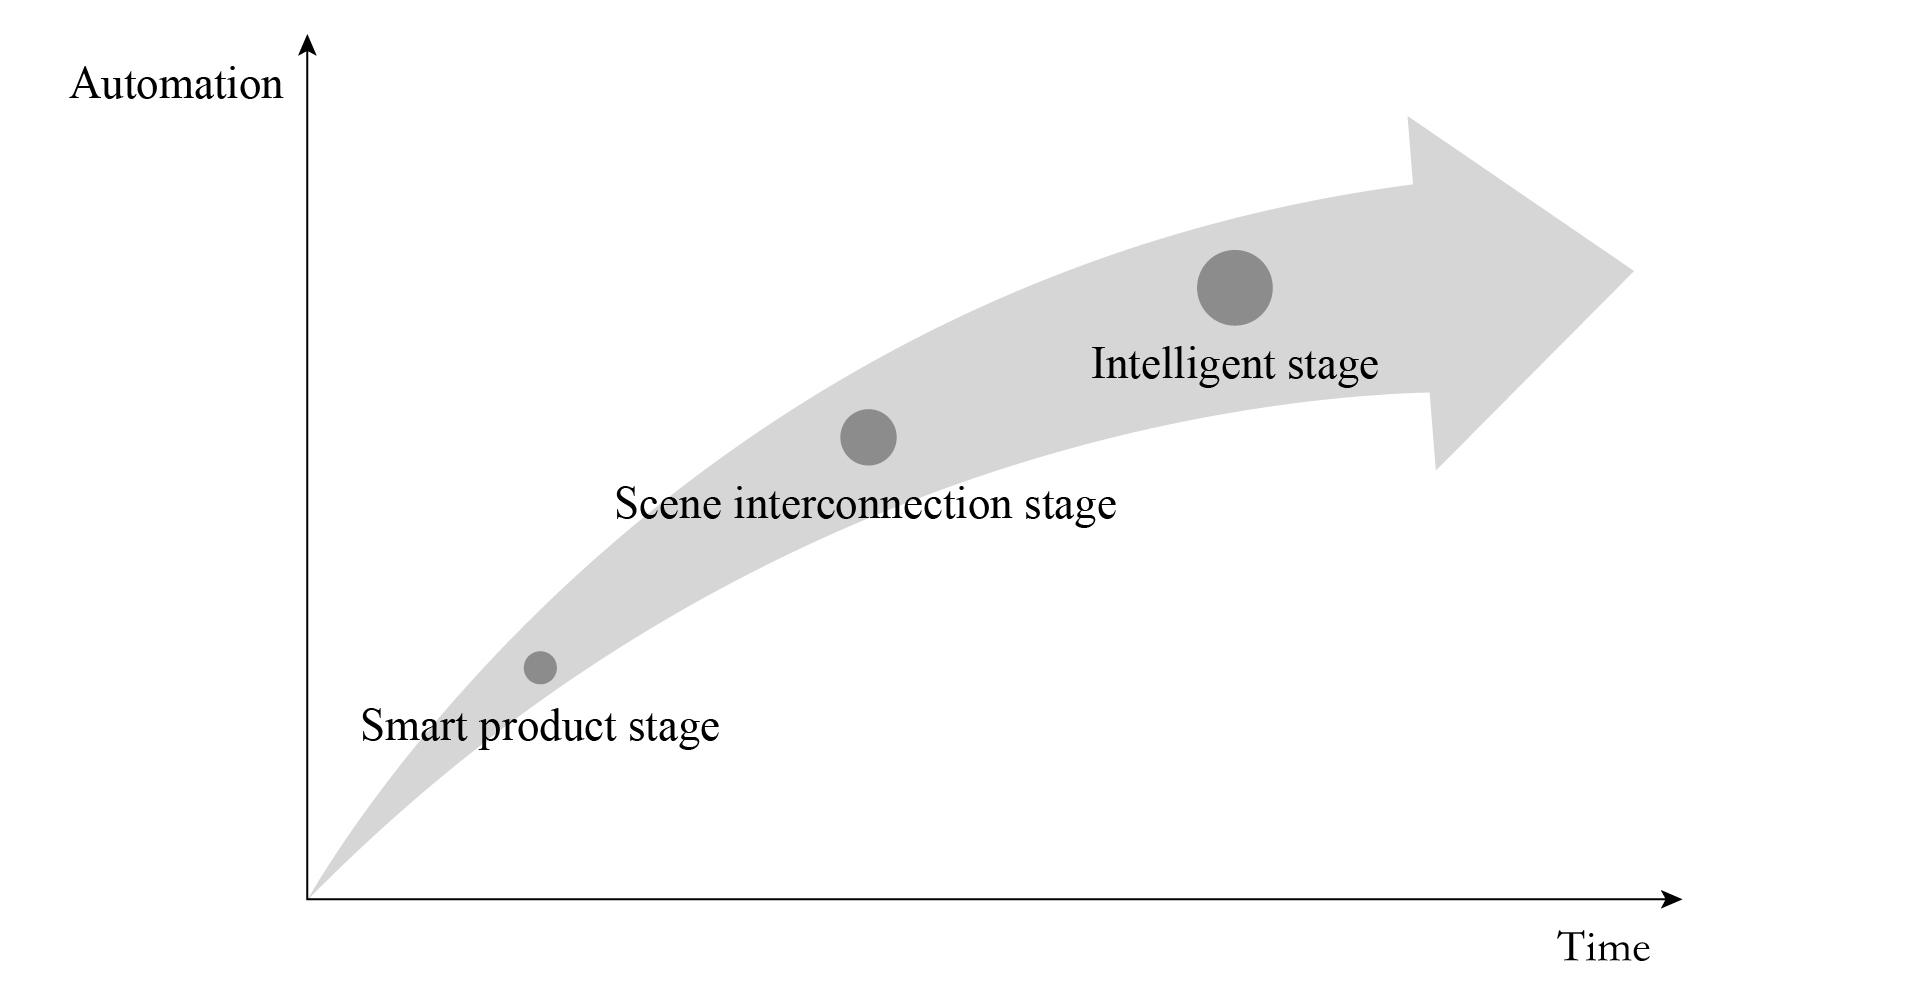
\includegraphics[width=0.8\textwidth]{D1Z/1-2}
    \caption{Development stage of smart home}
\end{figure}

The first stage is about \textbf{smart products}. Different from traditional homes, in smart homes, IoT devices receive signals with sensors, and are networked through wireless communication technologies such as Wi-Fi, Bluetooth LE, and ZigBee. Users can control smart products in a variety of ways, such as smartphone apps, voice assistants, smart speaker control, etc.

The second stage focuses on \textbf{scene interconnection}. In this stage, developers are no longer considering controlling single smart product, but interconnecting two or more smart products, automating to a certain extent, and finally forming a custom scene mode. For example, when the user presses any scene mode button, the lights, curtains, and air conditioners will be automatically adapted to the presets. Of course, there is the prerequisite that the linkage logic are readily set up, including trigger conditions and execution actions. Imagine that the air conditioning heating mode is triggered when the indoor temperature drops below 10°C; that at 7 o’clock in the morning, music is played to wake up the user, smart curtains are opened, and the rice cooker or bread toaster starts through a smart socket; as the user gets up and finishes washing, breakfast is already served, so that there will be no delay in going to work. How convenient has our life become!

The third stage goes to \textbf{intelligence stage}. As more smart home devices are accessed, so will the types of data generated. With the help of cloud computing, big data and artificial intelligence, it is like a “smarter brain” has been planted into smart homes, which no longer require frequent commands from the user. They collect data from previous interactions and learn the user's behaviour patterns and preferences, so as to automate activities, including providing recommendations for decision-making.

Currently, most smart homes are at the scene interconnection stage. As the penetration rate and intelligence of smart products increase, barriers between communication protocols are being removed. In the future, smart homes are bound to become really “smart”, just like the AI system Jarvis in \textit{Iron Man}, which can not only help the user control various devices, handle daily affairs, but also have super computing power and thinking ability. In the intelligent stage, human beings will receive better services both in quantity and quality.

\chapter[Introduction and Practice of IoT Projects]{\chaptertitle{Introduction and Practice of IoT Projects}{Introduction and Practice of IoT Projects}}

\vspace{24pt}
In Chapter 1, we introduced the architecture of IoT, and the roles and interrelationships of the perception \& control layer, network layer, platform layer, and application layer, as well as the development of smart home. However, just like when we learn to paint, knowing the theoretical knowledge is far from enough. We have to “get our hands dirty” to put IoT projects into practice in order to truly master the technology. In addition, when a project moves to the mass production stage, it is necessary to consider more factors such as network connection, configuration, IoT cloud platform interaction, firmware management and updates, mass production management, and security configuration.

So, what do we need to pay attention to when developing a complete IoT project?

In Chapter 1, we mentioned that smart home is one of the most common IoT application scenarios, and smart lights are one of the most basic and practical appliances, which can be used in homes, hotels, gyms, hospitals, etc. Therefore, in this book, we will take the construction of a smart light project as the starting point, explain its components and features, and provide guidance on project development. We hope that you can draw inferences from this case to create more IoT applications.

\section{Introduction to Typical IoT Projects}
In terms of development, basic functional modules of IoT projects can be classified into software and hardware development of IoT devices, client application development, and IoT cloud platform development. It is important to clarify the basic functional modules, which will be further described in this section.

\subsection{Basic Modules for Common IoT Devices}
Software and hardware development of IoT devices include the following basic modules:

\begin{term}{Data collection}
    As the bottom layer of the IoT architecture, the IoT devices of the perception \& control layer connect sensors and devices through their chips and peripherals to achieve data collection and operation control.
\end{term}

\vspace{12pt}
\begin{term}{Account binding and initial configuration}
    For most IoT devices, account binding and initial configuration are completed in one operational process, for example, connecting devices with users by configuring Wi-Fi network.
\end{term}

\begin{term}{Interaction with IoT cloud platforms}
    To monitor and control IoT devices, it is also necessary to connect them to IoT cloud platforms, in order to give commands and report status through interaction between each other.
\end{term}

\begin{term}{Device control}
    When connected with IoT cloud platforms, devices can communicate with the cloud and be registered, bound, or controlled. Users can query product status and carry out other operations on the smartphone app through IoT cloud platforms or local communication protocols.
\end{term}

\begin{term}{Firmware upgrade}
    IoT devices can also achieve firmware upgrade based on manufacturers’ needs. By receiving commands sent by the cloud, firmware upgrade and version management will be realized. With this firmware upgrade feature, you can continuously enhance the functions of IoT devices, fix defects, and improve user experience.
\end{term}

\subsection{Basic Modules of Client Applications}
Client applications (e.g., smartphone apps) mainly include the following basic modules:

\begin{term}{Account system and authorisation}
    It supports account and device authorisation.
\end{term}

\begin{term}{Device control}
    Smartphone apps are usually equipped with controlling functions. Users can easily connect to IoT devices, and manage them anytime, anywhere through smartphone apps. In a real-world smart home, devices are mostly controlled through smartphone apps, which not only enables intelligent management of devices, but also saves the cost of manpower. Therefore, device control is a must for client applications, such as device function attribute control, scene control, scheduling, remote control, device linkage, etc. Smart home users can also customise scenes according to personal needs, controlling lighting, home appliances, entrance, etc., to make home life more comfortable and convenient. They can time air conditioning, turn off it remotely, set the hallway light on automatically once the door is unlocked, or switch to the “theater” mode with one single button.
\end{term}

\begin{term}{Notification}
    Client applications update real-time status of IoT devices, and send alerts when devices go abnormal.
\end{term}

\begin{term}{After-sales customer service}
    Smartphone apps can provide after-sales services for products, to solve problems related to IoT device failures and technical operations in a timely manner.
\end{term}

\begin{term}{Featured functions}
    To meet the needs of different users, other functions may be added, such as Shake, NFC, GPS, etc. GPS can help set the accuracy of scene operations according to location and distance, while the Shake function allows users to set the commands to be executed for specific device or scene by shaking.
\end{term}

\subsection{Introduction to Common IoT Cloud Platforms}
IoT cloud platform is an all-in-one platform which integrates functions such as device management, data security communication, and notification management. According to their target group and accessibility, IoT cloud platforms can be divided into public IoT cloud platforms (hereinafter referred to as “\textbf{public cloud}”) and private IoT cloud platforms (hereinafter referred to as “\textbf{private cloud}”). 

Public cloud usually indicates shared IoT cloud platforms for enterprises or individuals, operated and maintained by platform providers, and shared through the Internet. It can be free or low-cost, and provides services throughout the open public network, such as Alibaba Cloud, Tencent Cloud, Baidu Cloud, AWS IoT, Google IoT, etc. As a supporting platform, public cloud can integrate upstream service providers and downstream end users to create a new value chain and ecosystem.

Private cloud is built for enterprise use only, thus guaranteeing the best control over data, security, and service quality. Its services and infrastructure are maintained separately by enterprises, and the supporting hardware and software are also dedicated to specific users. Enterprises can customise cloud services to meet the needs of their business. At present, some smart home manufacturers have already got private IoT cloud platforms and developed smart home applications based on them.

Public cloud and private cloud have their own advantages, which will be explained later.

To achieve communication connectivity, it is necessary to complete at least embedded development on the device side, alongwith business servers, IoT cloud platforms, and smartphone apps. Facing such a huge project, public cloud normally provides software development kits for device-side and smartphone apps to speed up the process. Both public and private cloud provide services including device access, device management, device shadow, and operation and maintenance.

\begin{term}{Device access}
    IoT cloud platforms need to provide not only interfaces for device access using protocols such as MQTT, CoAP, HTTPS, and WebSocket, but also the function of device security authentication to block forged and illegal devices, effectively reducing the risk of being compromised. Such authentication usually supports different mechanisms, so when devices are mass-produced, it is necessary to pre-assign the device certificate according to the selected authentication mechanism and burn it into the devices.
\end{term}

\begin{term}{Device management}
    The device management function provided by IoT cloud platforms can not only help manufacturers monitor the activation status and online status of their devices in real time, but also allows options such as adding / removing devices, retrieving, adding / deleting groups, firmware upgrade, and version management.
\end{term}

\begin{term}{Device shadow}
    IoT cloud platforms can create a persistent virtual version (device shadow) for each device, and the status of the device shadow can be synchronised and obtained by smartphone app or other devices through Internet transmission protocols. Device shadow stores the latest reported status and expected status of each device, and even if the device is offline, it can still obtain the status by calling APIs. Device shadow provides always-on APIs, which makes it easier to build smartphone apps that interact with devices.
\end{term}

\begin{term}{Operation and maintenance}
    The O\&M function includes three aspects: 
    \begin{itemize}
        \item Demonstrating statistical information about IoT devices and notifications.
        \item Log management allows information retrieval about device behavior, up / down message flow, and message content.
        \item Device debugging supports command delivery, configuration update, and checking the interaction between IoT cloud platforms and device messages.
    \end{itemize}
\end{term}

\section{Practice: Smart Light Project}
After the theoretical introduction in each chapter, you will find a practice section related to the Smart Light project to help you get hands-on experience. The project is based on Espressif’s ESP32-C3 chip and ESP RainMaker IoT Cloud Platform, and covers wireless module hardware in smart light products, embedded software for smart devices based on ESP32-C3, smartphone apps, and ESP RainMaker interaction.

\note[Source code]{
For better learning and developing experience, the project in this book has been open-sourced. You can download the source code from our GitHub repository at \url{https://github.com/espressif/book-esp32c3-iot-projects}.}

\subsection{Project Structure}
The Smart Light project consists of three parts:

\begin{enumerate}[label=\roman*.]
    \item \textbf{Smart light devices based on ESP32-C3}, responsible for interacting with IoT cloud platforms, and controlling the switch, brightness and color temperature of the LED lamp beads.
    \item \textbf{Smartphone apps} (including tablet apps running on Android and iOS), responsible for network configuration of smart light products, as well as querying and controlling their status.
    \item \textbf{An IoT cloud platform based on ESP RainMaker}. For simplification, we consider the IoT cloud platform and business server as a whole in this book. Details about ESP RainMaker will be provided in Chapter 3.
\end{enumerate}

The correspondence between the Smart Light project structure and the architecture of IoT is shown in Figure 2.1.

\begin{figure}[!ht]
    \centering
    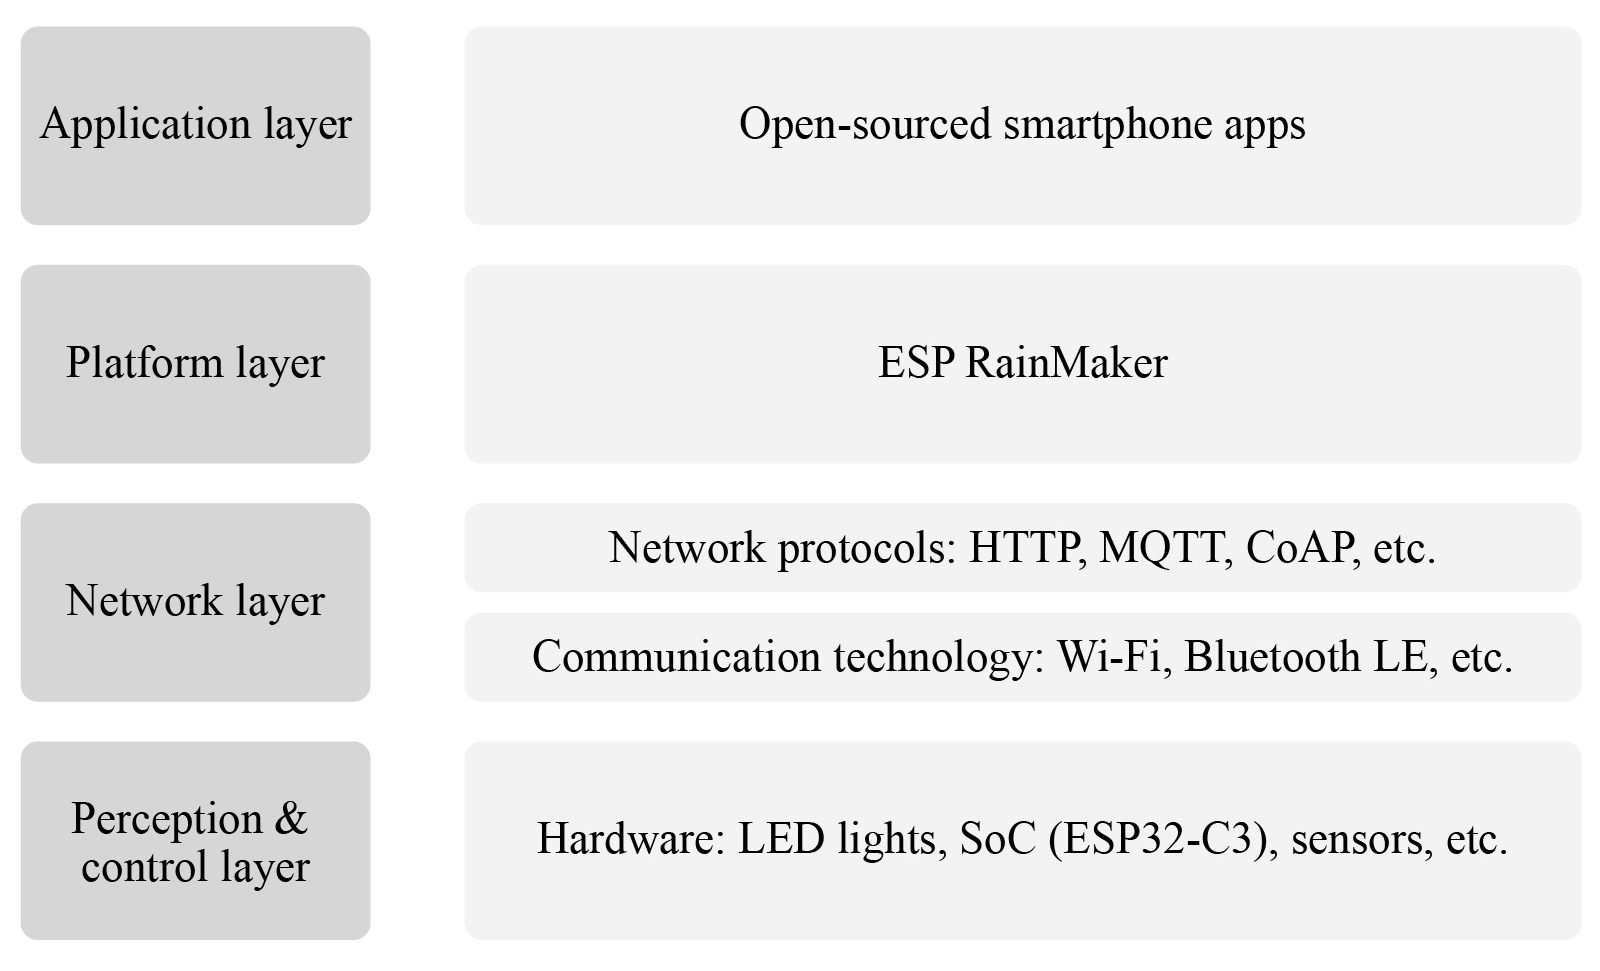
\includegraphics[width=0.7\textwidth]{D2Z/2-1}
    \caption{Structure of smart light project}
\end{figure}

\subsection{Project Functions}
Divided according to the structure, functions of each part are as follows.

\begin{term}{Smart light devices}
    \begin{itemize}
        \item Network configuration and connection.
        \item LED PWM control, such as switch, brightness, color temperature, etc.
        \item Automation or scene control, e.g., time switch.
        \item Encryption and secure boot of the Flash.
        \item Firmware upgrade and version management.
    \end{itemize}
\end{term}

\begin{term}{Smartphone apps}
    \begin{itemize}
        \item Network configuration and device binding.
        \item Smart light product control, such as switch, brightness, color temperature, etc.
        \item Automation or scene settings, e.g., time switch.
        \item Local/remote control.
        \item User registration, login, etc.
    \end{itemize}
\end{term}

\begin{term}{ESP RainMaker IoT cloud platform}
    \begin{itemize}
        \item Enabling IoT device access.
        \item Providing device operation APIs accessible to smartphone apps.
        \item Firmware upgrade and version management.
    \end{itemize}
\end{term}

\subsection{Hardware Preparation}
If interested in putting the project into practice, you will also need the following hardware: smart lights, smartphones, Wi-Fi routers, and a computer that meets the installation requirements of the development environment.

\begin{term}{Smart lights}
    Smart lights are a new type of bulbs, whose shape is the same as the general incandescent bulb. A smart light is composed of capacitor step-down regulated power supply, wireless module (with built-in ESP32-C3), LED controller and RGB LED matrix. When connected to power, the 15 V DC voltage output after capacitor step-down, diode rectification, and regulation provides energy to the LED controller and LED matrix. The LED controller can automatically send high and low levels at certain intervals, switching the RGB LED matrix between closed (lights on) and open (lights off), so that it can emit cyan, yellow, green, purple, blue, red, and white light. The wireless module is responsible for connecting to the Wi-Fi router, receiving and reporting the status of smart lights, and sending commands to control the LED.

    \begin{figure}[!ht]
        \centering
        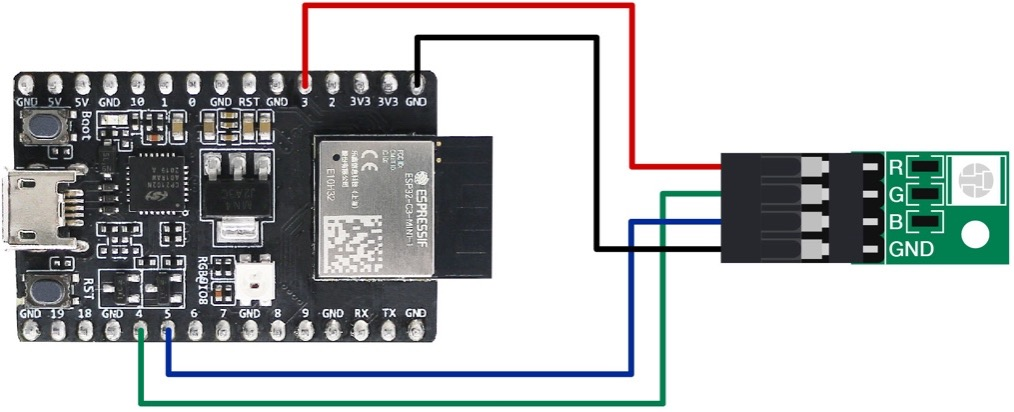
\includegraphics[width=0.6\textwidth]{D2Z/2-2}
        \caption{A simulated smart light}
    \end{figure}

    In the early development stage, you can simulate a smart light using the ESP32-C3-DevKitM-1 board connected with RGB LED lamp beads (see Figure 2.2). But you should note that this is not the only way to assemble a smart light. The hardware design of the project in this book only contains a wireless module (with built-in ESP32-C3), but not a complete smart light hardware design.

    \parskip 6pt
    In addition, Espressif also produces a ESP32-C3-based audio development board – ESP32-C3-Lyra – for controlling lights with audio. The board has interfaces for microphones and speakers and can control LED strips. It can be used for developing ultra-low-cost, high-performance audio broadcasters and rhythm light strips. Figure 2.3 shows a ESP32-C3-Lyra board linked with a strip of 40 LED lights.

    \begin{figure}[!ht]
        \centering
        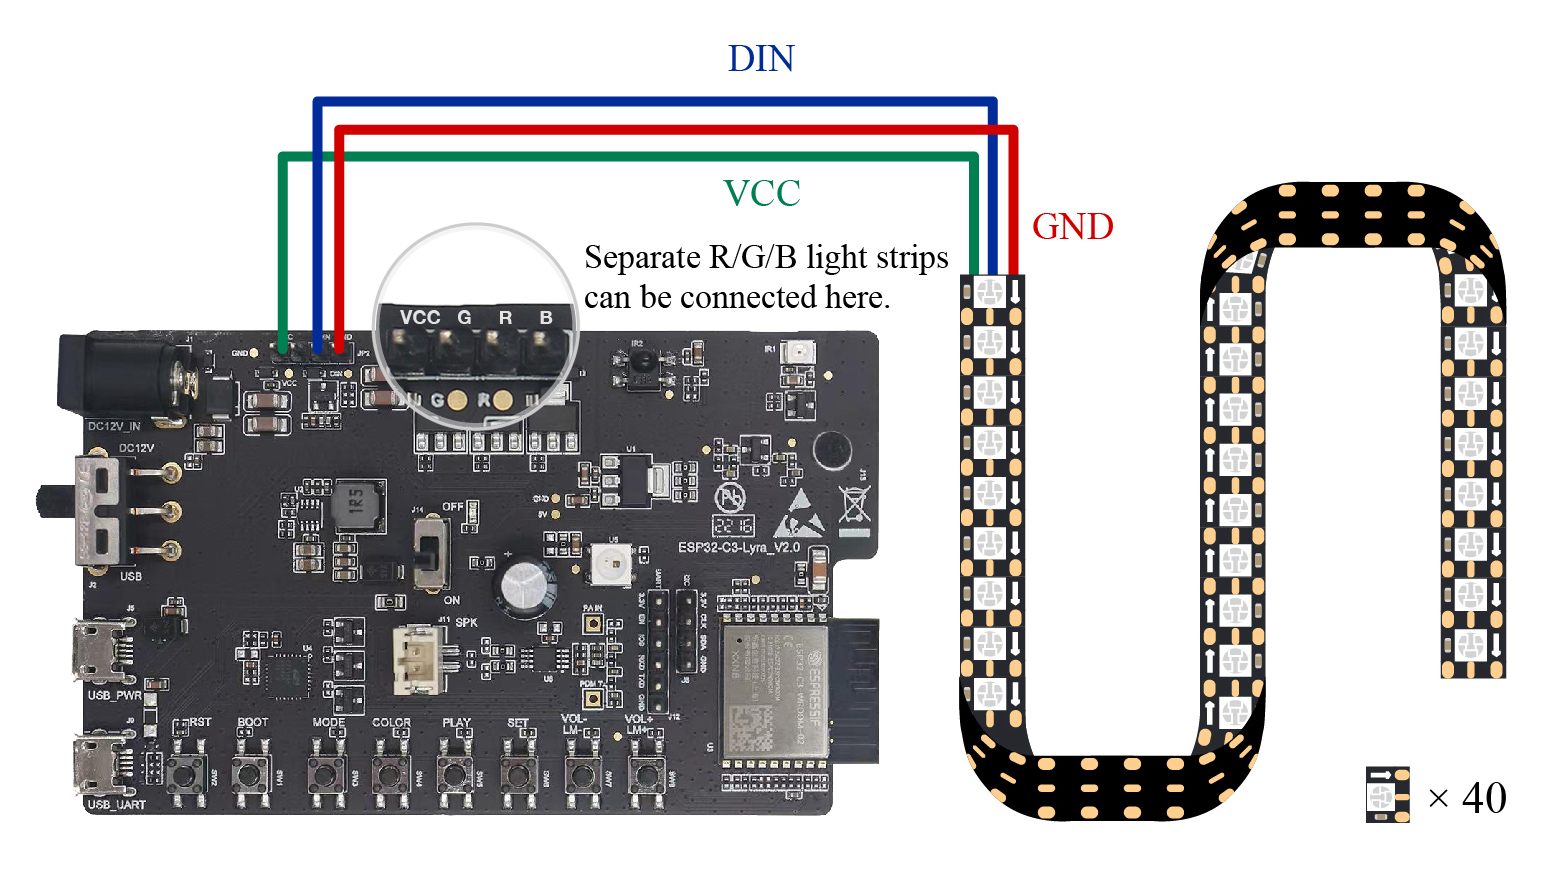
\includegraphics[width=0.75\textwidth]{D2Z/2-3}
        \caption{ESP32-C3-Lyra linked with a strip of 40 LED lights}
    \end{figure}
\end{term}

\begin{term}{Smartphones (Android/iOS)}
    The Smart Light project involves the development of a smartphone app for setting up and controlling smart light products.
\end{term}

\begin{term}{Wi-Fi routers}
    Wi-Fi routers convert wired network signals and mobile network signals into wireless network signals, for computers, smartphones, tablets, and other wireless devices to connect to the network. For example, broadband in the home only needs to be connected to a Wi-Fi router to achieve wireless networking of Wi-Fi devices. The mainstream protocol standard supported by Wi-Fi routers is IEEE 802.11n, with an average TxRate of 300 Mbps, or 600 Mbps at maximum. They are backward compatible with IEEE 802.11b and IEEE 802.11g. The ESP32-C3 chip by Espressif supports IEEE 802.11b/g/n, so you can choose a single-band (2.4 GHz) or dual-band (2.4 GHz and 5 GHz) Wi-Fi router.
\end{term}

\begin{term}{A computer (Linux/macOS/Windows)}
    Development environment will be introduced in Chapter 4.
\end{term}

\subsection{Development Process}
\begin{figure}[!ht]
        \centering
        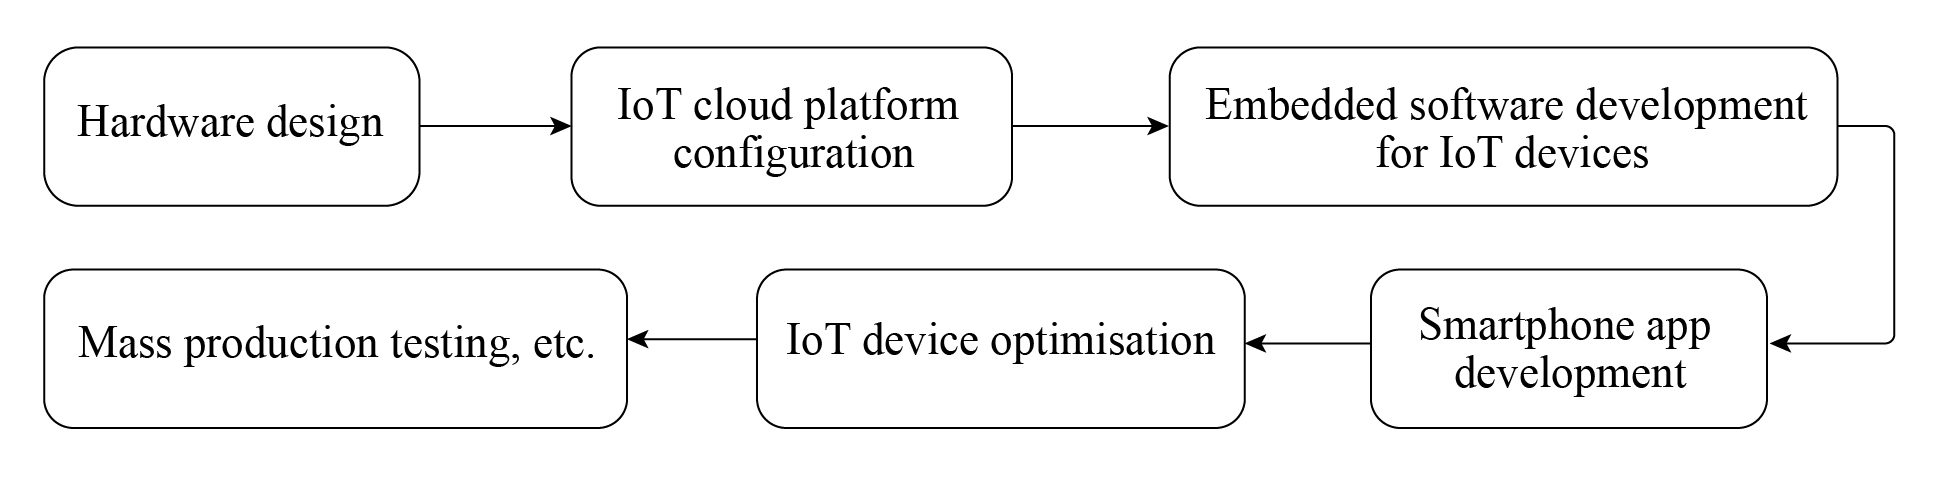
\includegraphics[width=0.8\textwidth]{D2Z/2-4}
        \caption{Steps of developing the Smart Light project}
\end{figure}

\begin{term}{Hardware design}
    Hardware design of IoT devices is essential to an IoT project. A complete smart light project is intended to produce a lamp working under mains supply. Different manufacturers produce lamps of different styles and driver types, but their wireless modules are usually of the same function. To simplify the development process of the Smart Ligh project, this book only covers the hardware design and software development of wireless modules.
\end{term}

\begin{term}{IoT cloud platform configuration}
    To use IoT cloud platforms, you need to configure projects on the backend, such as creating products, creating devices, setting device properties, etc.
\end{term}

\begin{term}{Embedded software development for IoT devices}
    Implement expected functions with ESP-IDF, Espressif’s device-side SDK, including connecting to IoT cloud platforms, developing LED drivers, and upgrading firmware.
\end{term}

\begin{term}{Smartphone app development}
    Develop smartphone apps for Android and iOS systems to realise user registration and login, device control and other functions.
\end{term}

\begin{term}{IoT device optimisation}
    Once the basic development of IoT device functions is completed, you may turn to optimisation tasks, such as power optimisation.
\end{term}

\begin{term}{Mass production testing}
    Carry out mass production tests according to related standards, such as equipment function test, aging test, RF test, etc.
\end{term}

Despite the steps listed above, a Smart Light project is not necessarily subject to such procedure as different tasks can also be carried out at the same time. For example, embedded software and smartphone apps can be developed in parallel. Some steps may also need to be repeated, such as IoT device optimisation and mass production testing.

\section{Summary}
In this chapter, we first expounded on the basic components and functional modules of an IoT project, then introduced the Smart Light case for practice, refering to its structure, functions, hardware preparation, and development process. Readers can draw inferences from the practice and become confident to carry out IoT projects with minimum mistakes in the future.

\chapter[Introduction to ESP RainMaker]{\chaptertitle{Introduction to ESP RainMaker}{Introduction to ESP RainMaker}}

\vspace{36pt}
The Internet of Things (IoT) offers endless possibilities to change the way people live, yet the development of IoT engineering is full of challenges. With public clouds, terminal manufacturers can implement product functionality through the following solutions:

\begin{term}{Based on solution providers’ cloud platforms}
    In this way, terminal manufacturers only need to design the product hardware, then connect the hardware to the cloud using provided communication module, and configure the product functions following the guidelines. This is an efficient approach since it eliminates the need for server-side and application-side development and operations and maintenance (O\&M). It allows terminal manufacturers to focus on hardware design without having to consider cloud implementation. However, such solutions (e.g., device firmware and App) are generally not open source, so the product functions will be limited by provider’s cloud platform which cannot be customized. Meanwhile, the user and device data also belong to the cloud platform.
\end{term}

\begin{term}{Based on cloud products}
    In this solution, after completing the hardware design, terminal manufacturers not only need to implement cloud functions using one or more cloud products provided by the public cloud, but also need to link the hardware with the cloud. For example, to connect to Amazon Web Services (AWS), terminal manufacturers need to use AWS products such as Amazon API Gateway, AWS IoT Core, and AWS Lambda to enable device access, remote control, data storage, user management, and other basic functions. It not only asks terminal manufacturers to flexibly use and configure cloud products with in-depth understanding and rich experience, but also requires them to consider the construction and maintenance cost for initial and later stages This poses great challenges to the company's energy and resources.
\end{term}

Compared with public clouds, private clouds are usually built for specific projects and products. Private cloud developers are given highest level of freedom in protocol design and business logic implementation. Terminal manufacturers can make products and design schemes at will, and easily integrate and empower user data. Combining the high security, scalability and reliability of public cloud with the advantages of private cloud, Espressif launched ESP RainMaker, a deeply integrated private cloud solution based on Amazon cloud. Users can deploy ESP RainMaker and build private cloud simply with an AWS account.

\section{What is ESP RainMaker?}
ESP RainMaker is a complete AIoT platform built with multiple mature AWS products. It provides various services required for mass production such as device cloud access, device upgrade, backend management, third-party login, voice integration, and user management. By using the Serverless Application Repository (SAR) provided by AWS, terminal manufacturers can quickly deploy ESP RainMaker to their AWS accounts, which is time-efficient and easy to operate. Managed and maintained by Espressif, the SAR used by ESP RainMaker helps developers reduce cloud maintenance costs and accelerate the development of AIoT products, thus building secure, stable, and customizable AIoT solutions. Figure 3.1 shows the architecture of ESP RainMaker.
\begin{figure}[!ht]
    \centering
    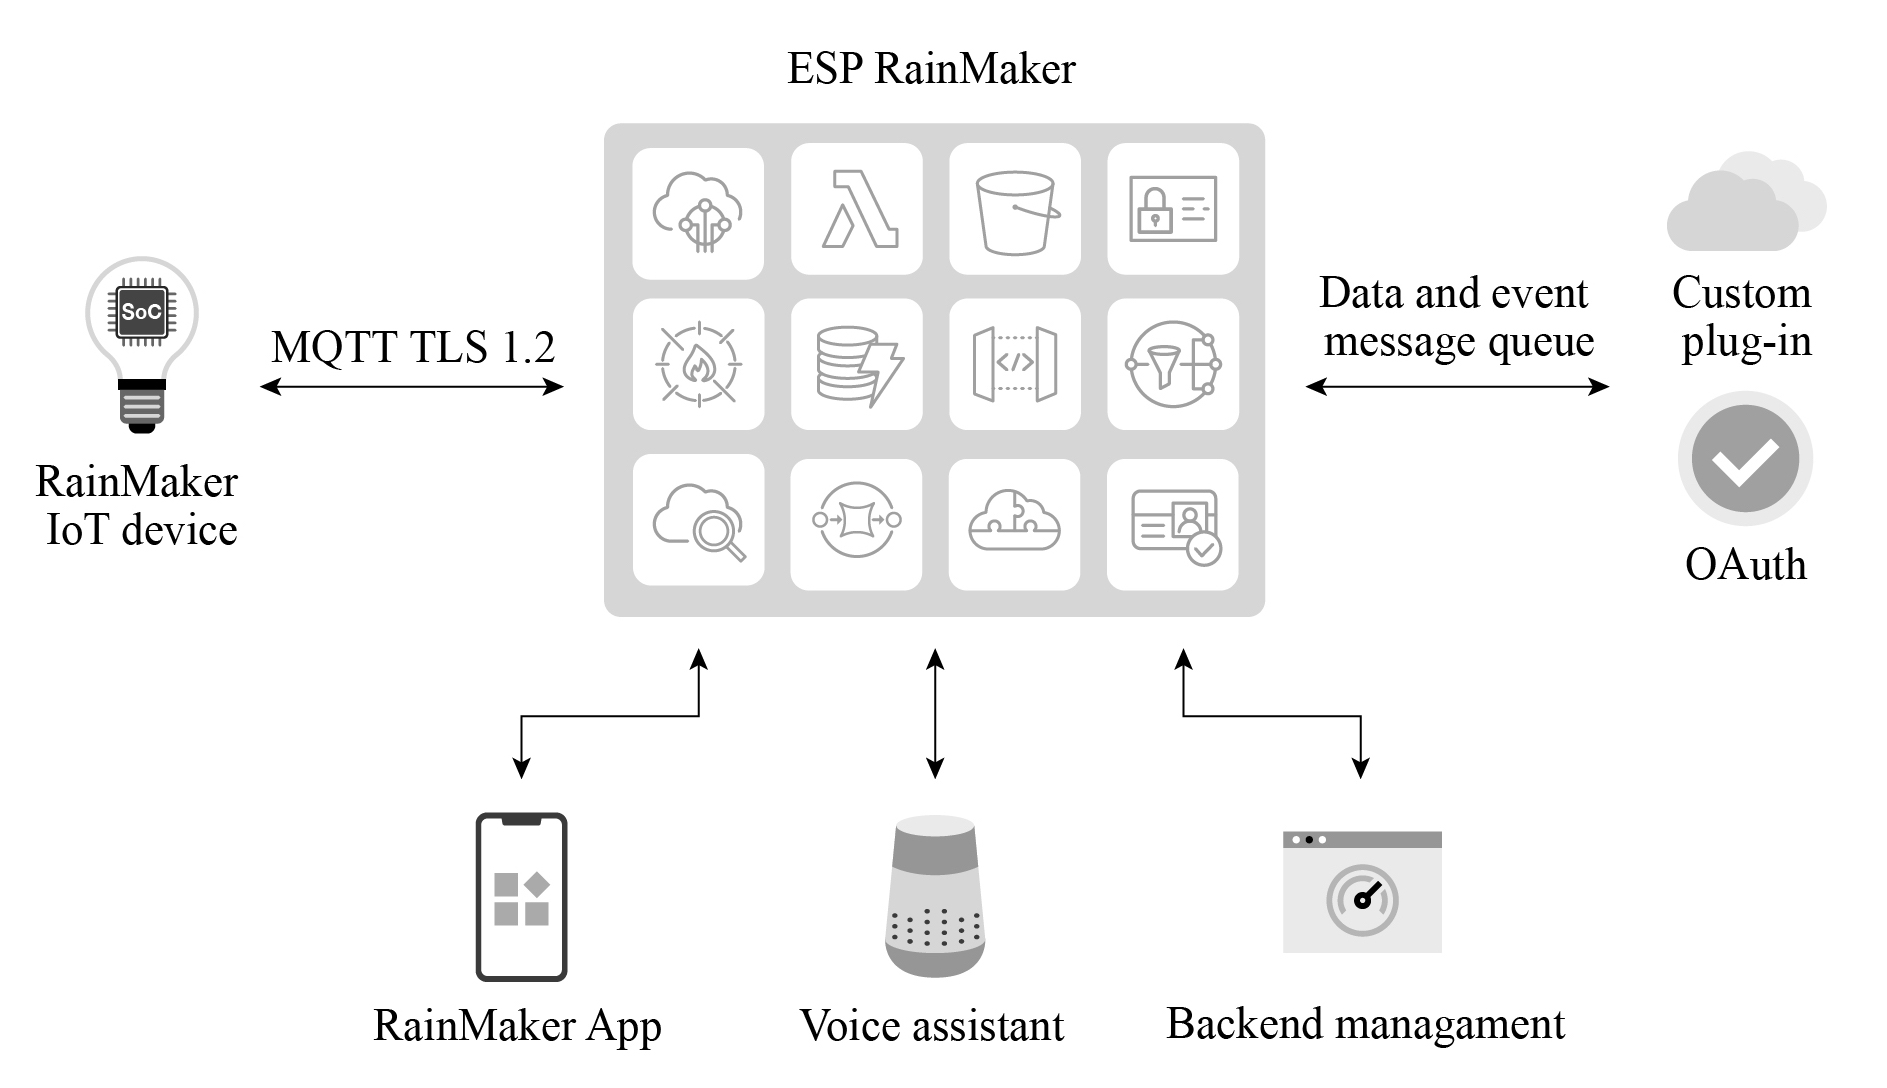
\includegraphics[width=0.85\textwidth]{D3Z/3-1}
    \caption{Architecture of ESP RainMaker}
\end{figure}

The ESP RainMaker public server by Espressif is free for all ESP enthusiasts, makers, and educators for solution evaluation. Developers can log in with Apple, Google, or GitHub accounts, and quickly build their own IoT application prototypes. The public server integrates Alexa and Google Home, and provides voice control services, which are supported by Alexa Skill and Google Actions. Its semantic recognition function is also powered by third parties. RainMaker IoT devices only respond to specific actions. For an exhaustive list of supported voice commands, please check the third-party platforms. In addition, Espressif offers a public RainMaker App for users to control the products through smartphones.

\section{The Implementation of ESP RainMaker}

As shown in Figure 3.2, ESP RainMaker consists of four parts:

\begin{itemize}
    \item \textbf{Claiming Service}, enabling RainMaker devices to dynamically obtain certificates.
    {\setlength{\parskip}{0pt}
    \item \textbf{RainMaker Cloud} (also known as cloud backend), providing services such as message filtering, user management, data storage, and third-party integrations.
    \item \textbf{RainMaker Agent}, enabling RainMaker devices to connect to RainMaker Cloud.
    \item \textbf{RainMaker Client} (RainMaker App or CLI scripts), for provisioning, user creation, device association and control, etc.}
\end{itemize}

\begin{figure}[h!]
    \centering
    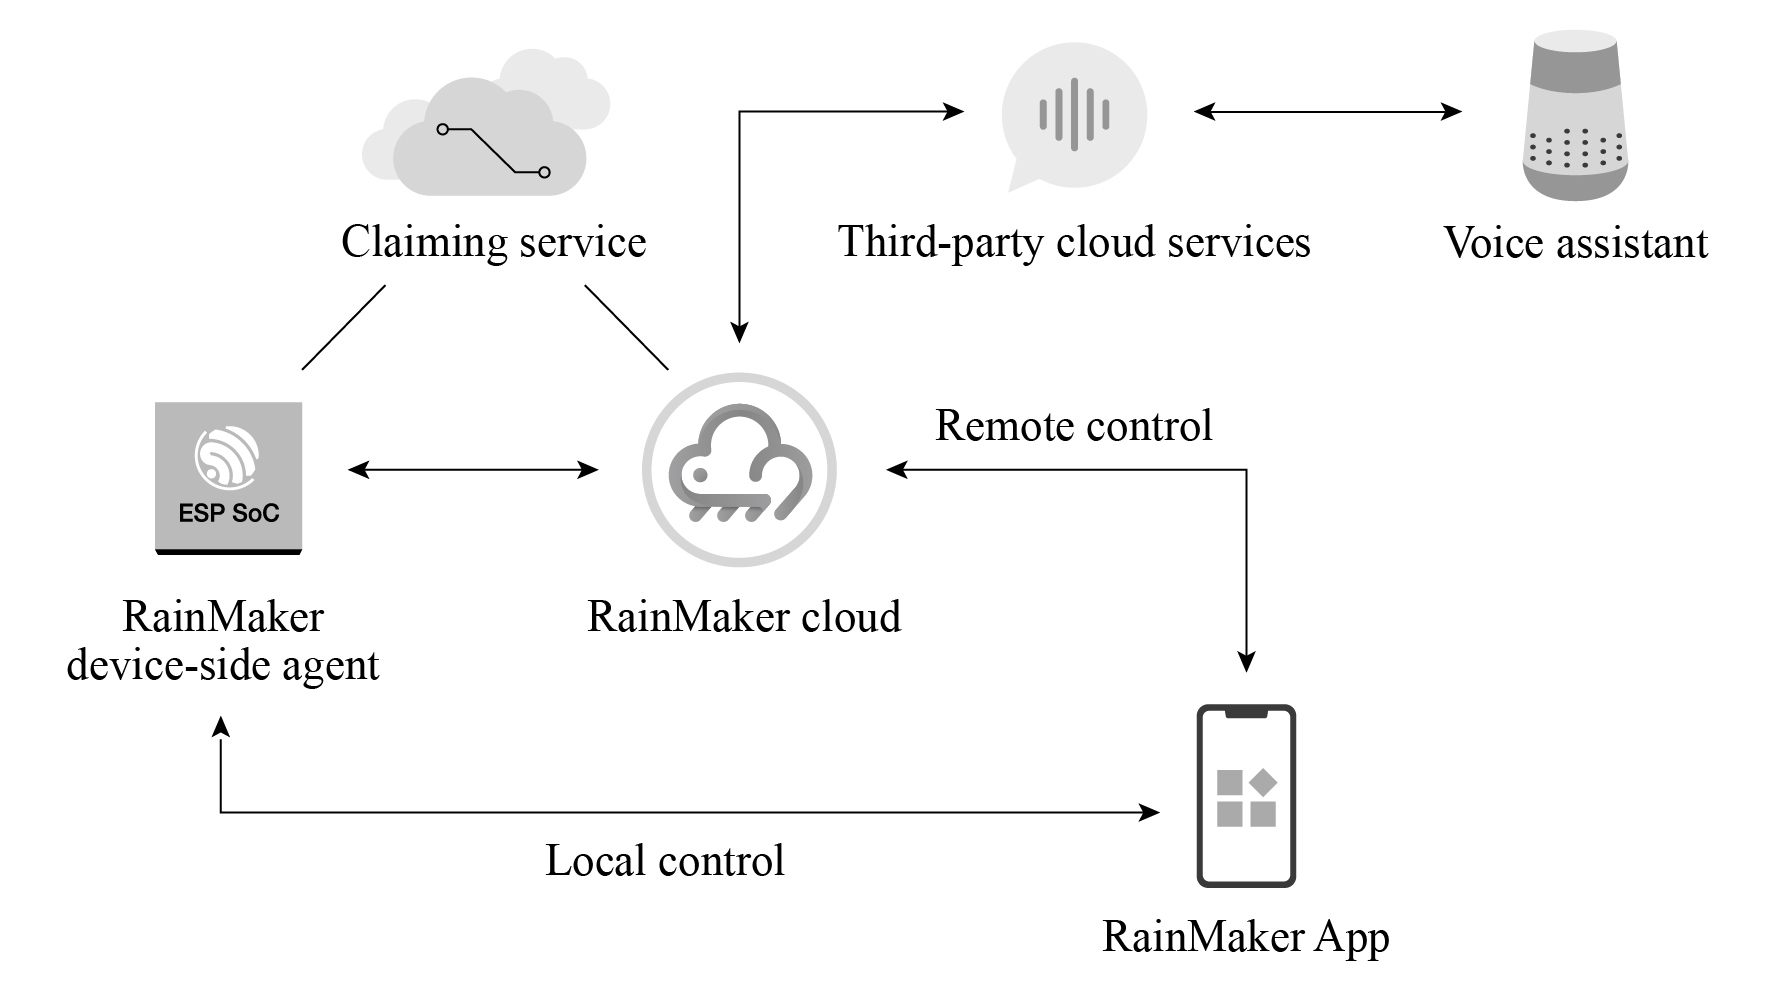
\includegraphics[width=0.75\textwidth]{D3Z/3-2}
    \caption{Structure of ESP RainMaker}
\end{figure}

ESP RainMaker provides a complete set of tools for product development and mass production, including:

\begin{term}{RainMaker SDK}
    RainMaker SDK is based on ESP-IDF and provides the source code of the device-side agent and related C APIs for firmware development. Developers only need to write the application logic and leave the rest to the RainMaker framework. For more information about C APIs, please visit \url{https://bookc3.espressif.com/rm/c-api-reference}.
\end{term}

\begin{term}{RainMaker App}
    The public version of RainMaker App allows developers to complete device provisioning, and control and query the status of devices (e.g., smart lighting products). It is available on both iOS and Android app stores. For more details, please refer to Chapter 10.
\end{term}

\begin{term}{REST APIs}
    REST APIs help users build their own applications similar to the RainMaker App. For more information, please visit \url{https://swaggerapis.rainmaker.espressif.com/}.
\end{term}

\begin{term}{Python APIs}
    A Python-based CLI, which comes with the RainMaker SDK, is provided to implement all functions similar to smartphone features. For more information about Python APIs, please visit \url{https://bookc3.espressif.com/rm/python-api-reference}.
\end{term}

\begin{term}{Admin CLI}
    Admin CLI, with higher level of access, is provided for ESP RainMaker private deployment to generate device certificates in bulk.
\end{term}

\subsection{Claiming Service}

 All communication between RainMaker devices and the cloud backend is carried out through MQTT+TLS. In the context of ESP RainMaker, “Claiming” is the process in which devices obtain certificates from the Claiming Service to connect to the cloud backend. Note that Claiming Service is only applicable to the public RainMaker service, while for private deployment, the device certificates need to be generated in bulk through Admin CLI. ESP RainMaker supports three types of Claiming Service:

\begin{term}{Self Claiming}
    The device itself fetches the certificates through a secret key pre-programmed in eFuse after connecting to the Internet.
\end{term}

\begin{term}{Host Driven Claiming}
    The certificates are obtained from the development host with the RainMaker account.
\end{term}

\begin{term}{Assisted Claiming}
    The certificates are obtained via smartphone applications during provisioning.
\end{term}

\subsection{RainMaker Agent}
\begin{figure}[h!]
    \centering
    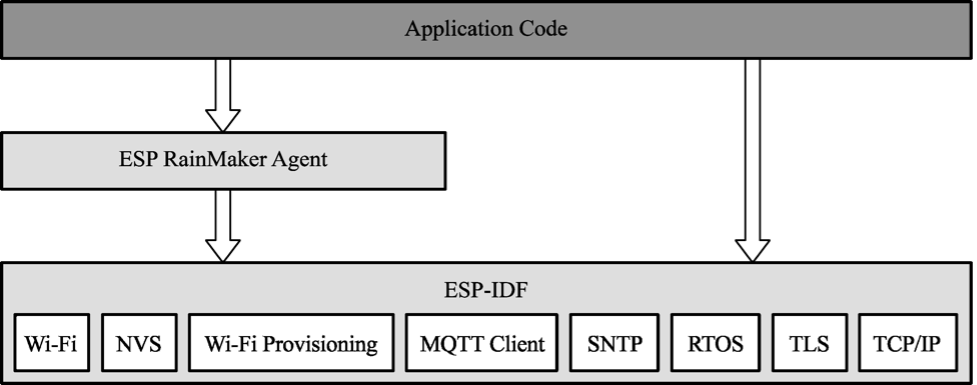
\includegraphics[width=0.8\textwidth]{D3Z/3-3}
    \caption{Structure of RainMaker SDK}
\end{figure}

The primary function of the RainMaker Agent is to provide connectivity and assist the application layer to process uplink/downlink cloud data. It is built through the RainMaker SDK and developed based on the proven ESP-IDF framework, using ESP-IDF components such as RTOS, NVS, and MQTT. Figure 3.3 shows the structure of the RainMaker SDK.

The RainMaker SDK includes two major features.

\textbf{Connection}
\begin{enumerate}[label=\roman*.]
    {
    \item Cooperating with Claiming Service to obtain device certificates.
    \item Connecting to the cloud backend using the secure MQTT protocol to provide remote connectivity and implement remote control, message reporting, user management, device management, etc. It uses the MQTT component in ESP-IDF by default and provides an abstraction layer to interface with other protocol stacks.
    \item Providing \texttt{wifi\_provisioning} component for Wi-Fi connection and provisioning, \texttt{esp\_https\_ota} component for OTA upgrades, and \texttt{esp\_local\_ctrl} component for local device discovery and connection. All these objectives can be achieved through simple configuration.
    
    }
\end{enumerate}

\textbf{Data processing}
\begin{enumerate}[label=\roman*.]
    {
    \item Storing the device certificates issued by Claiming Service and the data needed when running RainMaker, by default using the interface provided by the \texttt{nvs\_flash} component, and providing APIs for developers for direct use.
    \item Using the callback mechanism to process uplink/downlink cloud data and automatically unblocking the data to the application layer for easy processing by developers. For example, the RainMaker SDK provides rich interfaces for establishing TSL (Thing Specification Language) data, which are required to define TSL models to describe IoT devices and implement functions such as timing, countdown, and voice control. For basic interactive features such as timing, RainMaker SDK provides a development-free solution which can be simply enabled when needed. Then, the RainMaker Agent will directly process the data, send it to the cloud through the associated MQTT topic, and feed back the data changes in the cloud backend through callback mechanism.
    
    }
\end{enumerate}

\subsection{Cloud Backend}
The cloud backend is built on AWS Serverless Computing and achieved through AWS Cognito (identity management system), Amazon API Gateway, AWS Lambda (serverless computing service), Amazon DynamoDB (NoSQL database), AWS IoT Core (IoT access core that provides MQTT access and rule filtering), Amazon Simple Email Service (SES simple mail service), Amazon CloudFront (fast delivery network), Amazon Simple Queue Service (SQS message queuing), and Amazon S3 (bucket storage service). It is aimed to optimize scalability and security. With ESP RainMaker, developers can manage devices without having to write code in the cloud. Messages reported by devices are transparently transmitted to application clients or other third-party services.

Table 3.1 shows the AWS cloud products and functions used in the cloud backend, with more products and features under development.

\begin{table}[h!]
    \renewcommand{\arraystretch}{1.4}
    \caption{AWS cloud products and functions used by the cloud backend}
    \begin{tabular}{|>{\centering}m{0.28\textwidth}|m{0.7\textwidth}|}
        \hline
        \rowcolor{LightBlue}\textbf{AWS Cloud Product Used by RainMaker}&\multicolumn{1}{c|}{\textbf{Function}}\\
        \hline
        AWS Cognito&Managing user credentials and supporting third-party logins\\
        \hline
        AWS Lambda&Implementing the core business logic of the cloud backend\\
        \hline
        Amazon Timestream&Storing time series data\\
        \hline
        Amazon DynamoDB&Storing customers’ private information\\
        \hline
        AWS IoT Core&Supporting MQTT communication\\
        \hline
        Amazon SES&Providing email sending services\\
        \hline
        Amazon CloudFront&Accelerating the management of backend website access\\
        \hline
        Amazon SQS&Forwarding messages from AWS IoT Core\\
        \hline
    \end{tabular}
\end{table}

\subsection{RainMaker Client}
RainMaker clients, such as App and CLI, communicate with the cloud backend through REST APIs. Detailed information and instructions about REST APIs can be found in the Swagger documentation provided by Espressif. RainMaker's mobile application client is available for both iOS and Android systems. It allows device provisioning, control, and sharing, as well as creating and enabling countdown tasks and connecting to third-party platforms. It can automatically load UI and icons according to the configuration reported by the devices and fully display the device TSL.

For example, if a smart light is built on the RainMaker SDK-provided examples, the icon and UI of the bulb light will be loaded automatically when the provisioning is completed. Users can change the color and brightness of the light through the interface and achieve third-party control by linking Alexa Smart Home Skill or Google Smart Home Actions to their ESP RainMaker accounts. Figure 3.4 shows the icon and UI examples of the bulb light respectively on Alexa, Google Home, and ESP RainMaker App.

\newpage
\begin{figure}[h!]
\Centering
\begin{subfigure}{0.45\textwidth}
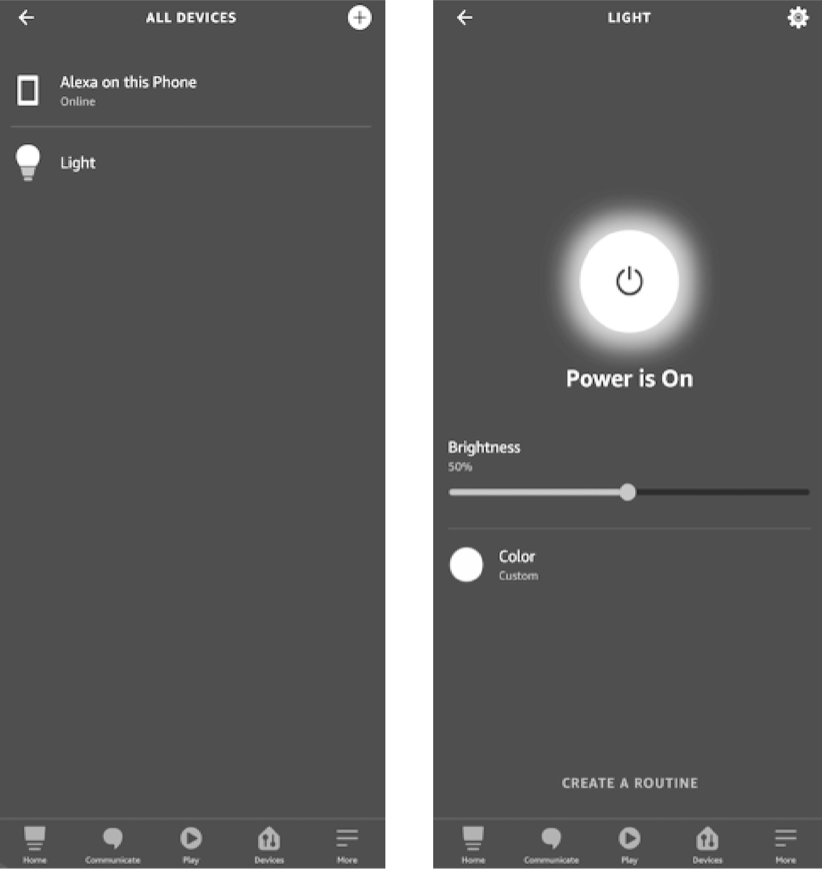
\includegraphics[width=\textwidth]{D3Z/3-4-a} 
\caption{Example - Alexa}
\end{subfigure}\hspace{1em}
\begin{subfigure}{0.5\textwidth}
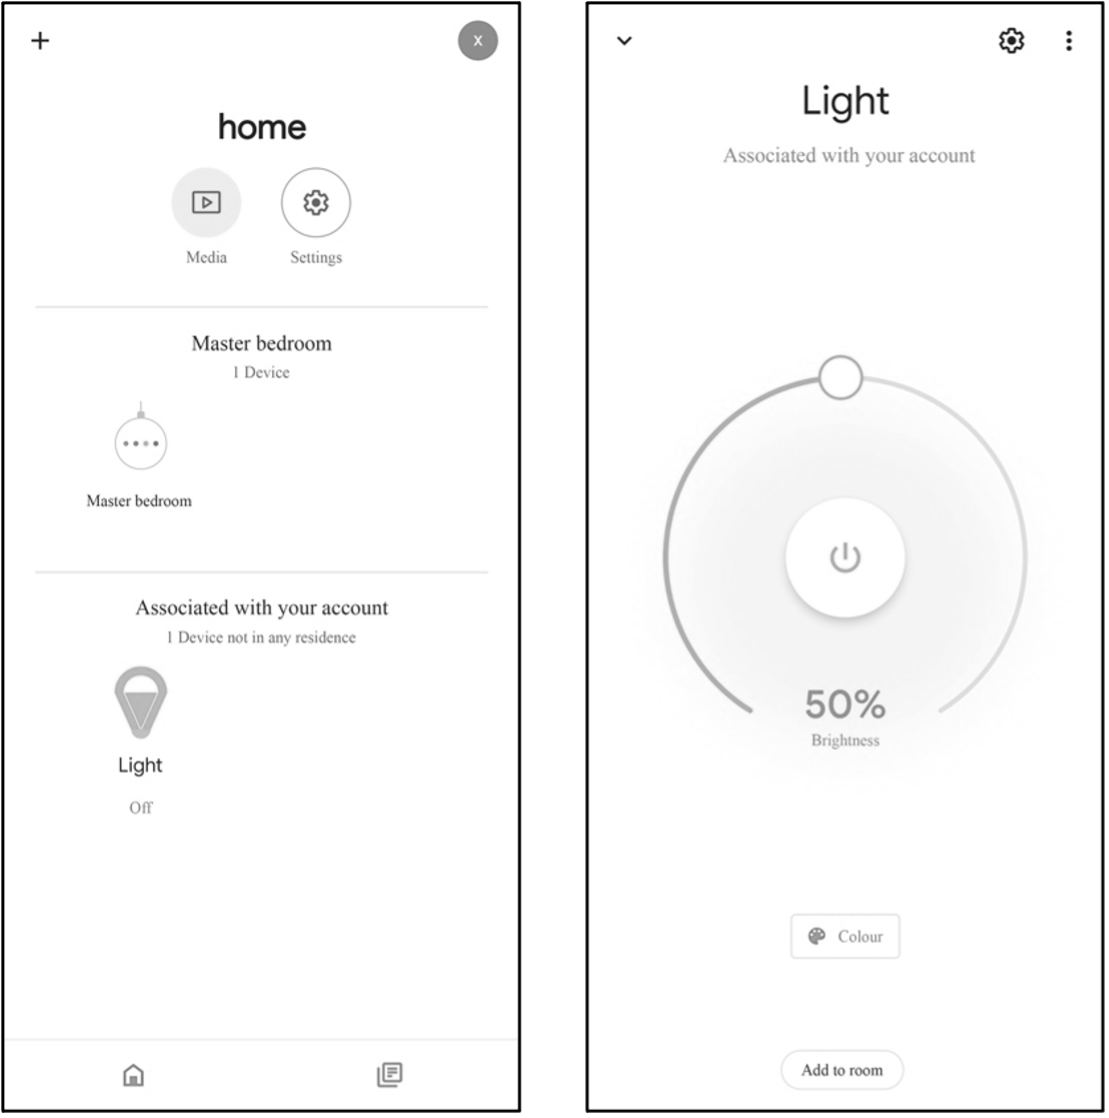
\includegraphics[width=0.95\textwidth]{D3Z/3-4-b}
\caption{Example - Google Home}
\end{subfigure}

\vspace{6pt}
\begin{subfigure}{0.55\textwidth}
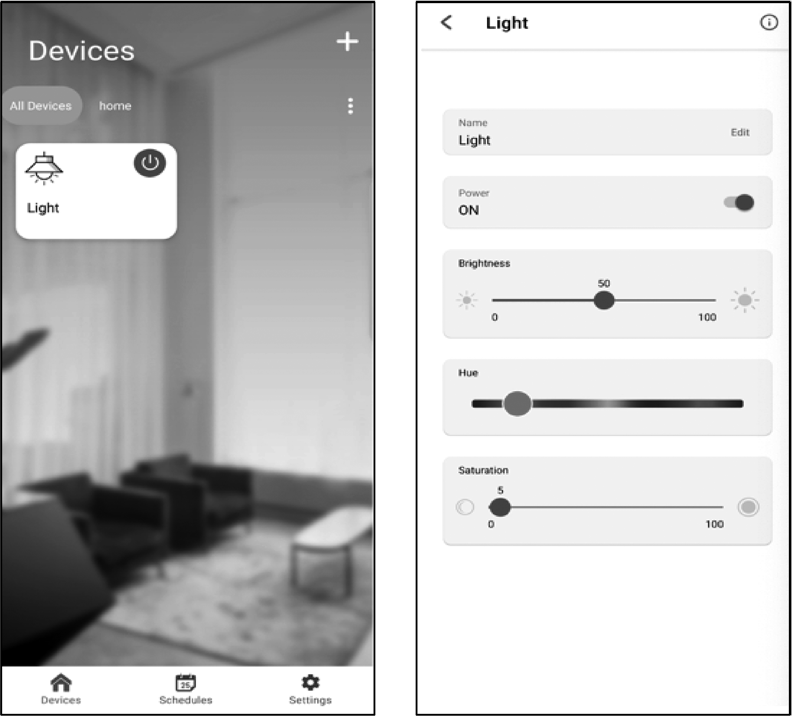
\includegraphics[width=\textwidth]{D3Z/3-4-c}
\caption{Example - ESP RainMaker}
\end{subfigure}
\caption{\Centering Examples of icon and UI of the bulb light on Alexa, Google Home, and ESP RainMaker App}
\end{figure}

\section{Practice: Key Points for Developing with ESP RainMaker}
Once the device driver layer has been completed, developers may start to create TSL models and process downlink data using the APIs provided by RainMaker SDK, and enable the ESP RainMaker basic services based on the product definition and requirements.

Section 9.4 of this book will explain the implementation of the LED smart light in RainMaker. During debugging, developers can use the CLI tools in the RainMaker SDK to communicate with the smart light (or call REST APIs from Swagger).

Chapter 10 will elaborate the usage of REST APIs in developing smartphone applications. The OTA upgrades of LED smart lights will be covered in Chapter 11. If developers have enabled the ESP Insights remote monitoring, the ESP RainMaker management backend will display the ESP Insights data. Details will be presented in Chapter 15.

ESP RainMaker supports \textbf{private deployment}, which differs from the public RainMaker server in the following ways:

\begin{term}{Claiming Service}
    To generate certificates in private deployments, it is required to use the RainMaker Admin CLI instead of Claiming. With public server, developers must be given admin rights to implement firmware upgrade, but it is undesirable in commercial deployments. Therefore, neither separate authentication service can be provided for self-claiming, nor admin rights for host driven or assisted claiming.
\end{term}

\begin{term}{Phone apps}
    In private deployments, applications need to be configured and compiled separately to ensure that the account systems are not interoperable.
\end{term}

\begin{term}{3rd party logins and voice integration}
    Developers have to configure separately via Google and Apple Developer accounts to enable 3rd party logins, as well as the Alexa Skill and Google Voice Assistant integration.
\end{term}

\note[TIPS]{For details about cloud deployment, please visit \url{https://customer.rainmaker.espressif.com}. In terms of firmware, migration from public server to private server only requires replacing device certificates, which greatly improves migration efficiency and reduces the cost of migration and secondary debugging.}

\section{Features of ESP RainMaker}
ESP RainMaker features are mainly targeted at three aspect - user management, end users, and admins. All features are supported in both public and private servers unless otherwise stated.

\subsection{User Management}
The user management features allow end users to register, log in, change passwords, retrieve passwords, etc.

\begin{term}{Register and log in}
    The registration and login methods supported by RainMaker include:

    \begin{itemize}
        \item Email id + Password
        \item Phone number + Password
        \item Google account
        \item Apple account
        \item GitHub account (public server only)
        \item Amazon account (private server only)
    \end{itemize}
\end{term}

\note{Sign up using Google/Amazon shares the user's email address with RainMaker. Sign up using Apple shares a dummy address that Apple assigns for the user specifically for the RainMaker service. A RainMaker account will be automatically created for users signing in with a Google, Apple, or Amazon account for the first time.}

\begin{term}{Change password}
    Valid only for Email id/Phone number based logins. All other active sessions will be logged out after password is changed. As per AWS Cognito behaviour, the logged-out sessions can stay active upto 1 hour.
\end{term}

\begin{term}{Retrieve password}
    Valid only for Email id/Phone number based logins.
\end{term}

\subsection{End User Features}
Features open to end users include local and remote control and monitoring, scheduling, device grouping, device sharing, push notifications, and third-party integrations.

\begin{term}{Remote control and monitoring}
    \begin{itemize}
        \item Query configuration, parameter values, and connection status for one or all devices.
        \item Set parameters for single or multiple devices.
    \end{itemize}
\end{term}

\begin{term}{Local control and monitoring}
    Mobile phone and the device need to be connected to the same network for local control.
\end{term}

\begin{term}{Scheduling}
    \begin{itemize}
        \item Users pre-set certain actions at a specific time.
        \item No Internet connection required for the device while executing the schedule.
        \item One time or repeat (by specifying days) for single or multiple devices.
    \end{itemize}
\end{term}

\begin{term}{Device grouping}
    Supports multi-level abstract grouping Group metadata can be used to create a Home - Room structure.
\end{term}

\begin{term}{Device sharing}
    One or more devices can be shared with one or more users.
\end{term}

\begin{term}{Push notifications}
    End users will receive push notifications for events such as
    \begin{itemize}
        \item New device(s) added/removed
        \item Device connected to cloud
        \item Device disconnected from cloud
        \item Device sharing requests created/accepted/declined
        \item Alert messages reported by devices
    \end{itemize}
\end{term}

\begin{term}{Third party integrations}
    Alexa and Google Voice Assistant are supported to control RainMaker devices, including lights, switches, sockets, fans, and temperature sensors.
\end{term}

\subsection{Admin Features}
Admin features allow administrators to implement device registration, device grouping, and OTA upgrades, and to view statistics and ESP Insights data.

\begin{term}{Device registration}
    Generate device certificates and register with Admin CLI (private server only).
\end{term}

\begin{term}{Device grouping}
    Create abstract or structured groups based on device information (private server only).
\end{term}

\begin{term}{Over-the-Air (OTA) upgrades}
    Upload firmware based on version and model, to one or more devices or a group Monitor, cancel, or archive OTA jobs.
\end{term}

\begin{term}{View statistics}
    Viewable statistics include:
    \begin{itemize}
        \item Device registrations (certificates registered by the admin)
        \item Device activations (device connected for the first time)
        \item User accounts
        \item User-device association
    \end{itemize}
\end{term}

\begin{term}{View ESP Insights data}
    Viewable ESP Insights data include:
    \begin{itemize}
        \item Errors, warnings, and custom logs
        \item Crash reports and analysis
        \item Reboot reasons
        \item Metrics like memory usage, RSSI, etc.
        \item Custom metrics and variables
    \end{itemize}
\end{term}

\section{Summary}
In this chapter, we introduced some key differences between the public RainMaker deployment and the private deployment. The private ESP RainMaker solution launched by Espressif is highly reliable and extensible. All ESP32 series chips have been connected and adapted to AWS, which greatly reduces the cost. Developers can focus on prototype verification without having to learn about AWS cloud products. We also explained the implementation and features of ESP RainMaker, and some key points for development using the platform.

\begin{figure}[h!]
    \Centering
    \begin{subfigure}{0.45\textwidth}
        \RaggedLeft
        
\includegraphics[height=0.7\textwidth]{D3Z/Android} 
    \end{subfigure}\hspace{40pt}
    \begin{subfigure}{0.45\textwidth}
        \RaggedRight
        
\includegraphics[height=0.7\textwidth]{D3Z/iOS}
    \end{subfigure}
\end{figure}

\begin{tabular}{>{\Centering}m{20em} >{\Centering}m{18em}}
\small{Scan to download ESP RainMaker for Android}&\small{Scan to download ESP RainMaker for iOS}
\end{tabular}

\chapter[Setting Up Development Environment]{\chaptertitle{Setting Up Development Environment}{Setting Up\newline Development Environment}}

\vspace{36pt}
This chapter focuses on ESP-IDF, the official software development framework for ESP32-C3. We’ll explain how to set up the environment on various operating systems, and introduce the project structure and build system of ESP-IDF, as well as the usage of related development tools. Then we’ll present the compiling and running process of an example project, while offering a detailed explanation of the output log at each stage.

\section{ESP-IDF Overview}
ESP-IDF (Espressif IoT Development Framework) is a one-stop IoT development framework provided by Espressif Technology. It uses C/C++ as the main development language and supports cross-compilation under mainstream operating systems such as Linux, Mac, and Windows. The example programs included in this book are developed using ESP-IDF, which offers the following features:

\begin{itemize}[leftmargin=1.5em]
    \item \textbf{SoC system-level drivers}. ESP-IDF includes drivers for ESP32, ESP32-S2, ESP32-C3, and other chips. These drivers encompass peripheral low level (LL) library, hardware abstraction layer (HAL) library, RTOS support and upper-layer driver software, etc.
    \item \textbf{Essential components}. ESP-IDF incorporates fundamental components required for IoT development. This includes multiple network protocol stacks such as HTTP and MQTT, a power management framework with dynamic frequency modulation, and features like Flash Encryption and Secure Boot, etc.
    \item \textbf{Development and production tools}. ESP-IDF provides commonly used tools for building, flash, and debugging during development and mass production (see Figure \ref{Building, flashing, and debugging tools for development and mass production}), such as the building system based on CMake, the cross-compilation tool chain based on GCC, and the JTAG debugging tool based on OpenOCD, etc.
\end{itemize}

\begin{figure}[h!]
    \centering
    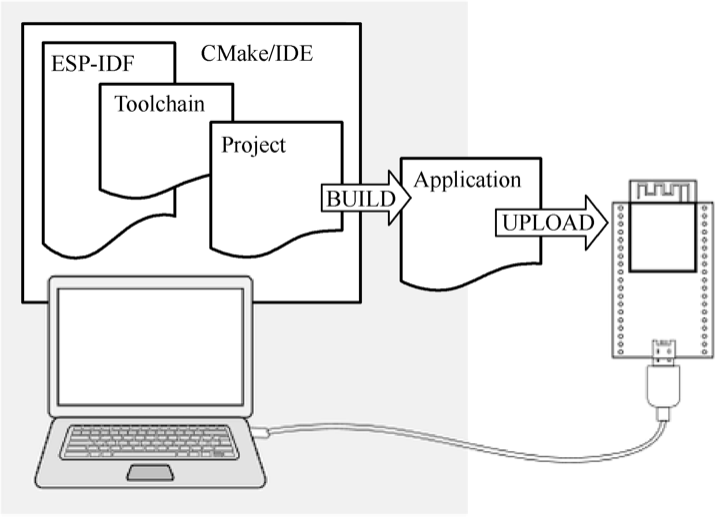
\includegraphics[width=0.6\textwidth]{D4Z/4-1}
    \caption{\Centering Building, flashing, and debugging tools for development and mass production}
    \label{Building, flashing, and debugging tools for development and mass production}
\end{figure}

It is worth noting that the ESP-IDF code primarily adheres to the the Apache 2.0 open-source license. Users can develop personal or commercial software without restrictions while complying with the terms of the open-source license. Additionally, users are granted permanent patent licenses free of charge, without the obligation to open-source any modifications made to the source code.

\subsection{ESP-IDF Versions}
The ESP-IDF code is hosted on GitHub as an open-source project. Currently, there are three major versions available: v3, v4, and v5. Each major version usually contains various sub-versions, such as v4.2, v4.3, and so on. Espressif Systems ensures a 30-month support for bug fixes and security patches for each released sub-version. Therefore, revisions of sub-versions are also released regularly, such as v4.3.1, v4.2.2, etc. Table 4.1 shows the support status of different ESP-IDF versions for Espressif chips, indicating whether they are in a preview stage (offering support for preview versions, which may lack certain features or documentation) or are officially supported.

\begin{table}[h!]
    \renewcommand{\arraystretch}{1.5}
    \caption{Support status of different ESP-IDF versions for Espressif chips}
    \begin{tabular}{|>{\Centering}m{5.5em}|>{\Centering}m{6.3em}|>{\Centering}m{6.3em}|>{\Centering}m{6.3em}|>{\Centering}m{6.3em}|>{\Centering}m{6.3em}|}
        \hline
        \rowcolor{LightBlue} \textbf{Series}&\textbf{v4.1}&\textbf{v4.2}&\textbf{v4.3}&\textbf{v4.4}&\textbf{v5.0}\\
        \hline
        ESP32&supported&supported&supported&supported&supported\\
        \hline
        ESP32-S2&&supported&supported&supported&supported\\
        \hline
        ESP32-C3&&&supported&supported&supported\\
        \hline
        ESP32-S3&&&&supported&supported\\
        \hline
        ESP32-C2&&&&&supported\\
        \hline
        ESP32-H2&&&&preview&preview\\
        \hline
    \end{tabular}
\end{table}

The iteration of major versions often involves adjustments to the framework structure and updates to the compilation system. For example, the major change from v3.* to v4.* was the gradual migration of the build system from Make to CMake. On the other hand, iteration of minor versions typically entails the addition of new features or support for new chips.

It is important to distinguish and understand the relationship between stable versions and GitHub branches. Versions labeled as v*.* or v*.*.* represent stable versions that have passed complete internal testing by Espressif. Once fixed, the code, tool chain, and release documents for the same version remain unchanged. However, GitHub branches (e.g., the \verb|release/v4.3| branch) undergo frequent code commits, often on a daily basis. Therefore, two code snippets under the same branch may differ, necessitating developers to promptly update their code accordingly.

\subsection{ESP-IDF Git Workflow}

Espressif follows a specific Git workflow for ESP-IDF, outlined as follows:

\begin{itemize}[leftmargin=1.5em]
    \item New changes are made on the \verb|master| branch, which serves as the main development branch. The ESP-IDF version on the \verb|master| branch always carries a \verb|-dev| tag to indicate that it is currently under development, such as \verb|v4.3-dev|. Changes on the \verb|master| branch will first be reviewed and tested in Espressif’s internal repository, and then pushed to GitHub after automated testing is complete.
    \item Once a new version has completed feature development on the \verb|master| branch and met the criteria for entering beta testing, it transitions to a new branch, such as \verb|release/|\\ \verb|v4.3|. In addition, this new branch is tagged as a pre-release version, like \verb|v4.3-beta1|. Developers can refer to the GitHub platform to access the complete list of branches and tags for ESP-IDF. It’s important to note that the beta version (pre-release version) may still have a significant number of known issues. As the beta version undergoes continuous testing, bug fixes are added to both this version and the \verb|master| branch simultaneously. Meanwhile, the \verb|master| branch may have already begun developing new features for the next version. When testing is nearly complete, a release candidate (\verb|rc|) label is added to the branch, indicating that it is a potential candidate for the official release, such as \verb|v4.3-rc1|. At this stage, the branch remains a pre-release version.
    \item If no major bugs are discovered or reported, the pre-release version eventually receives a major version label (e.g., v5.0) or a minor version label (e.g., v4.3) and becomes an official release version, which is documented in the release notes page. Subsequently, any bugs identified in this version are fixed on the release branch. After manual testing is completed, the branch is assigned a bug-fix version label (e.g., v4.3.2), which is also reflected on the release notes page.
\end{itemize}

\subsection{Choosing a Suitable Version}
Since ESP-IDF officially began supporting ESP32-C3 from version v4.3, and v4.4 has not yet been officially released at the time of writing this book, the version used in this book is v4.3.2, which is a revised version of v4.3. However, it is important to note that by the time you read this book, v4.4 or newer versions may already be available. When selecting a version, we recommend the following:

\begin{itemize}[leftmargin=1.5em]
    \item For \textbf{entry-level developers}, it is advisable to choose the stable v4.3 version or its revised version, which aligns with the example version used in this book.
    \item For \textbf{mass production} purposes, it is recommended to use the latest stable version to to benefit from the most up-to-date technical support.
    \item If you intend to experiment with \textbf{new chips} or explore \textbf{new product features}, please use the \verb|master| branch. The latest version contains all the latest features, but keep in mind that there may be known or unknown bugs present.
    \item If the stable version being used does not include the desired new features and you wish to \textbf{minimise the risks} associated with the \verb|master| branch, consider using the corresponding release branch, such as the \verb|release/v4.4| branch. Espressif’s GitHub repository will first create the \verb|release/v4.4| branch and subsequently release the stable v4.4 version based on a specific historical snapshot of this branch, after completing all feature development and testing.
\end{itemize}

\subsection{Overview of ESP-IDF SDK Directory}
The ESP-IDF SDK consists of two main directories: \verb|esp-idf| and \verb|.espressif|. The former contains ESP-IDF repository’s source code files and compilation scripts, while the latter mainly stores compilation tool chains and other software. Familiarity with these two directories will help developers make better use of available resources and speed up the development process. The directory structure of ESP-IDF is described below:

\begin{enumerate}[label=(\arabic*),leftmargin=2em]
    \item \textbf{ESP-IDF repository code directory} (\texttt{$\sim$/esp/esp-idf}), as shown in Figure \ref{ESP-IDF repository code directory}.

    \begin{figure}[h!]
        \centering
        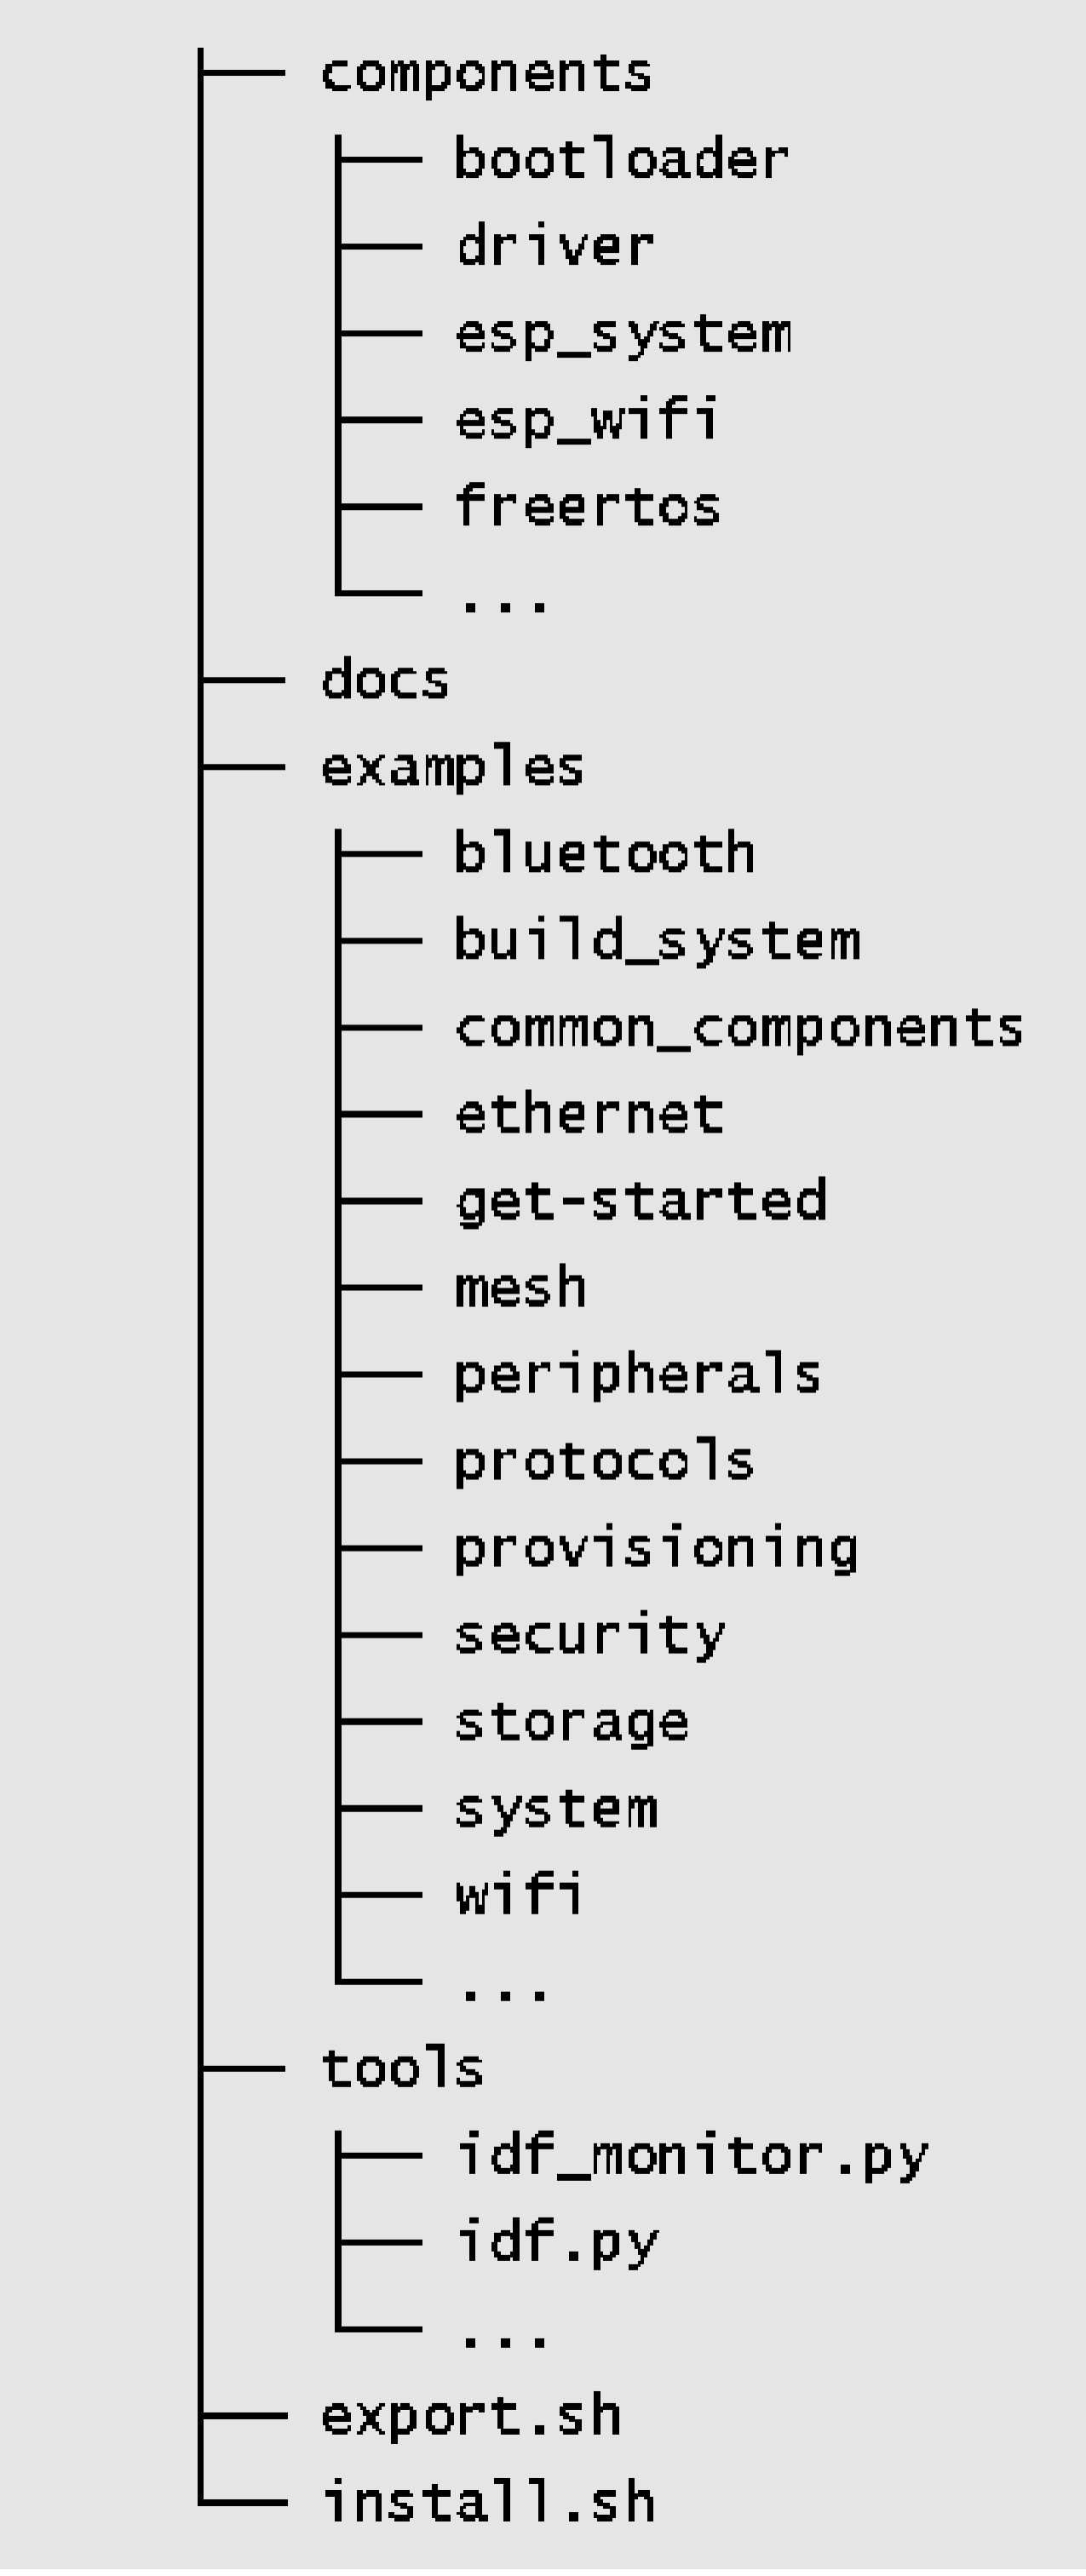
\includegraphics[width=0.35\textwidth]{D4Z/4-2}
        \caption{ESP-IDF repository code directory}
        \label{ESP-IDF repository code directory}
    \end{figure}

    \begin{enumerate}[label=\textbf{\alph*.},leftmargin=0em]
        \item \textbf{Component directory \texttt{components}}

        This core directory integrates numerous essential software components of ESP-IDF. No project code can be compiled without relying on the components within this directory. It includes driver support for various Espressif chips. From the LL library and HAL library interfaces for peripherals to the upper-level Driver and Virtual File System (VFS) layer support, developers can choose the appropriate components at different levels for their development needs. ESP-IDF also supports multiple standard network protocol stacks such as TCP/IP, HTTP, MQTT, WebSocket, etc. Developers can utilise familiar interfaces like Socket to build network applications. Components provide comprehensive functionality and can be easily integrated into applications, allowing developers to focus solely on the business logic. Some common components include:

        \begin{itemize}[leftmargin=1em]
            \item \verb|driver|: This component contains peripheral driver programs for various Espressif chip series, such as GPIO, I2C, SPI, UART, LEDC (PWM), etc. The peripheral driver programs in this component offer chip-independent abstract interfaces. Each peripheral has a common header file (such as \verb|gpio.h|), eliminating the need to deal with different chip-specific support questions.
            \item \verb|esp_wifi|: Wi-Fi, as a special peripheral, is treated as a separate component. It includes multiple APIs such as initialisation of various Wi-Fi driver modes, parameter configuration, and event processing. Certain functions of this component are provided in the form of static link libraries. ESP-IDF also provides comprehensive driver documentation for ease of use.
            \item \verb|freertos|: This component contains the complete FreeRTOS code. Apart from providing comprehensive support for this operating system, Espressif has also extended its support to dual-core chips. For dual-core chips like ESP32 and ESP32-S3, users can create tasks on specific cores.
        \end{itemize}

        \item \textbf{Document directory \texttt{docs}}

        This directory contains ESP-IDF related development documents, including the Get Started Guide, API Reference Manual, Development Guide, etc.

        \secnote{After being compiled by automated tools, the contents of this directory are deployed at \url{https://docs.espressif.com/projects/esp-idf}. Please ensure to switch the document target to ESP32-C3 and select the specified ESP-IDF version.}

        \item \textbf{Script tool \texttt{tools}}

        This directory contains commonly used compilation front-end tools such as \verb|idf.py|, and the monitor terminal tool \verb|idf_monitor.py|, etc. The sub-directory \verb|cmake| also contains core script files of the compilation system, serving as the foundation for implementing ESP-IDF compilation rules. When adding the environment variables, the contents within the \verb|tools| directory are added to the system environment variable, allowing \verb|idf.py| to be executed directly under the project path.

        \item \textbf{Example program directory \texttt{examples}}

        This directory comprises a vast collection of ESP-IDF example programs that demonstrate the usage of component APIs. The examples are organised into various sub-directories based on their categories:

        \begin{itemize}[leftmargin=1em]
            \item \verb|get-started|: This sub-directory includes entry-level examples like “hello world” and “blink” to help users grasp the basics.
            \item \verb|bluetooth|: You can find Bluetooth related examples here, including Bluetooth LE Mesh, Bluetooth LE HID, BluFi, and more.
            \item \verb|wifi|: This sub-directory focuses on Wi-Fi examples, including basic programs like Wi-Fi SoftAP, Wi-Fi Station, \verb|espnow|, as well as proprietary communication protocol examples from Espressif. It also includes multiple application layer examples based on Wi-Fi, such as Iperf, Sniffer, and Smart Config.
            \item \verb|peripherals|: This extensive sub-directory is further divided into numerous sub-folders based on peripheral names. It mainly contains peripheral driver examples for Espressif chips, with each example featuring several sub-examples. For instance, the \verb|gpio| sub-directory includes two examples: GPIO and GPIO matrix keyboard. It’s important to note that not all examples in this directory are applicable to ESP32-C3.  For example, the examples in \verb|usb/host| are only applicable to peripherals with USB Host hardware (such as ESP32-S3), and ESP32-C3 does not have this peripheral. The compilation system typically provides prompts when setting the target. The README file of each example lists the supported chips.
            \item \verb|protocols|: This sub-directory contains examples for various communication protocols, including MQTT, HTTP, HTTP Server, PPPoS, Modbus, mDNS, SNTP, covering a wide range of communication protocol examples required for IoT development.
            \item \verb|provisioning|: Here, you’ll find provisioning examples for different methods, such as Wi-Fi provisioning and Bluetooth LE provisioning.
            \item \verb|system|: This sub-directory includes system debugging examples (e.g., stack tracing, runtime tracing, task monitoring), power management examples (e.g., various sleep modes, co-processors), and examples related to common system components like console terminal, event loop, and system timer.
            \item \verb|storage|: Within this sub-directory, you’ll discover examples of all file systems and storage mechanisms supported by ESP-IDF (such as reading and writing of Flash, SD card and other storage media), as well as examples of non-volatile storage (NVS), FatFS, SPIFFS and other file system operations.
            \item \verb|security|: This sub-directory contains examples related to flash encryption.
        \end{itemize}
    \end{enumerate}

    \item \textbf{ESP-IDF compilation tool chain directory} (\texttt{$\sim$/.espressif}), as shown in Figure \ref{ESP-IDF compilation tool chain directory}.

    \begin{figure}[h!]
        \centering
        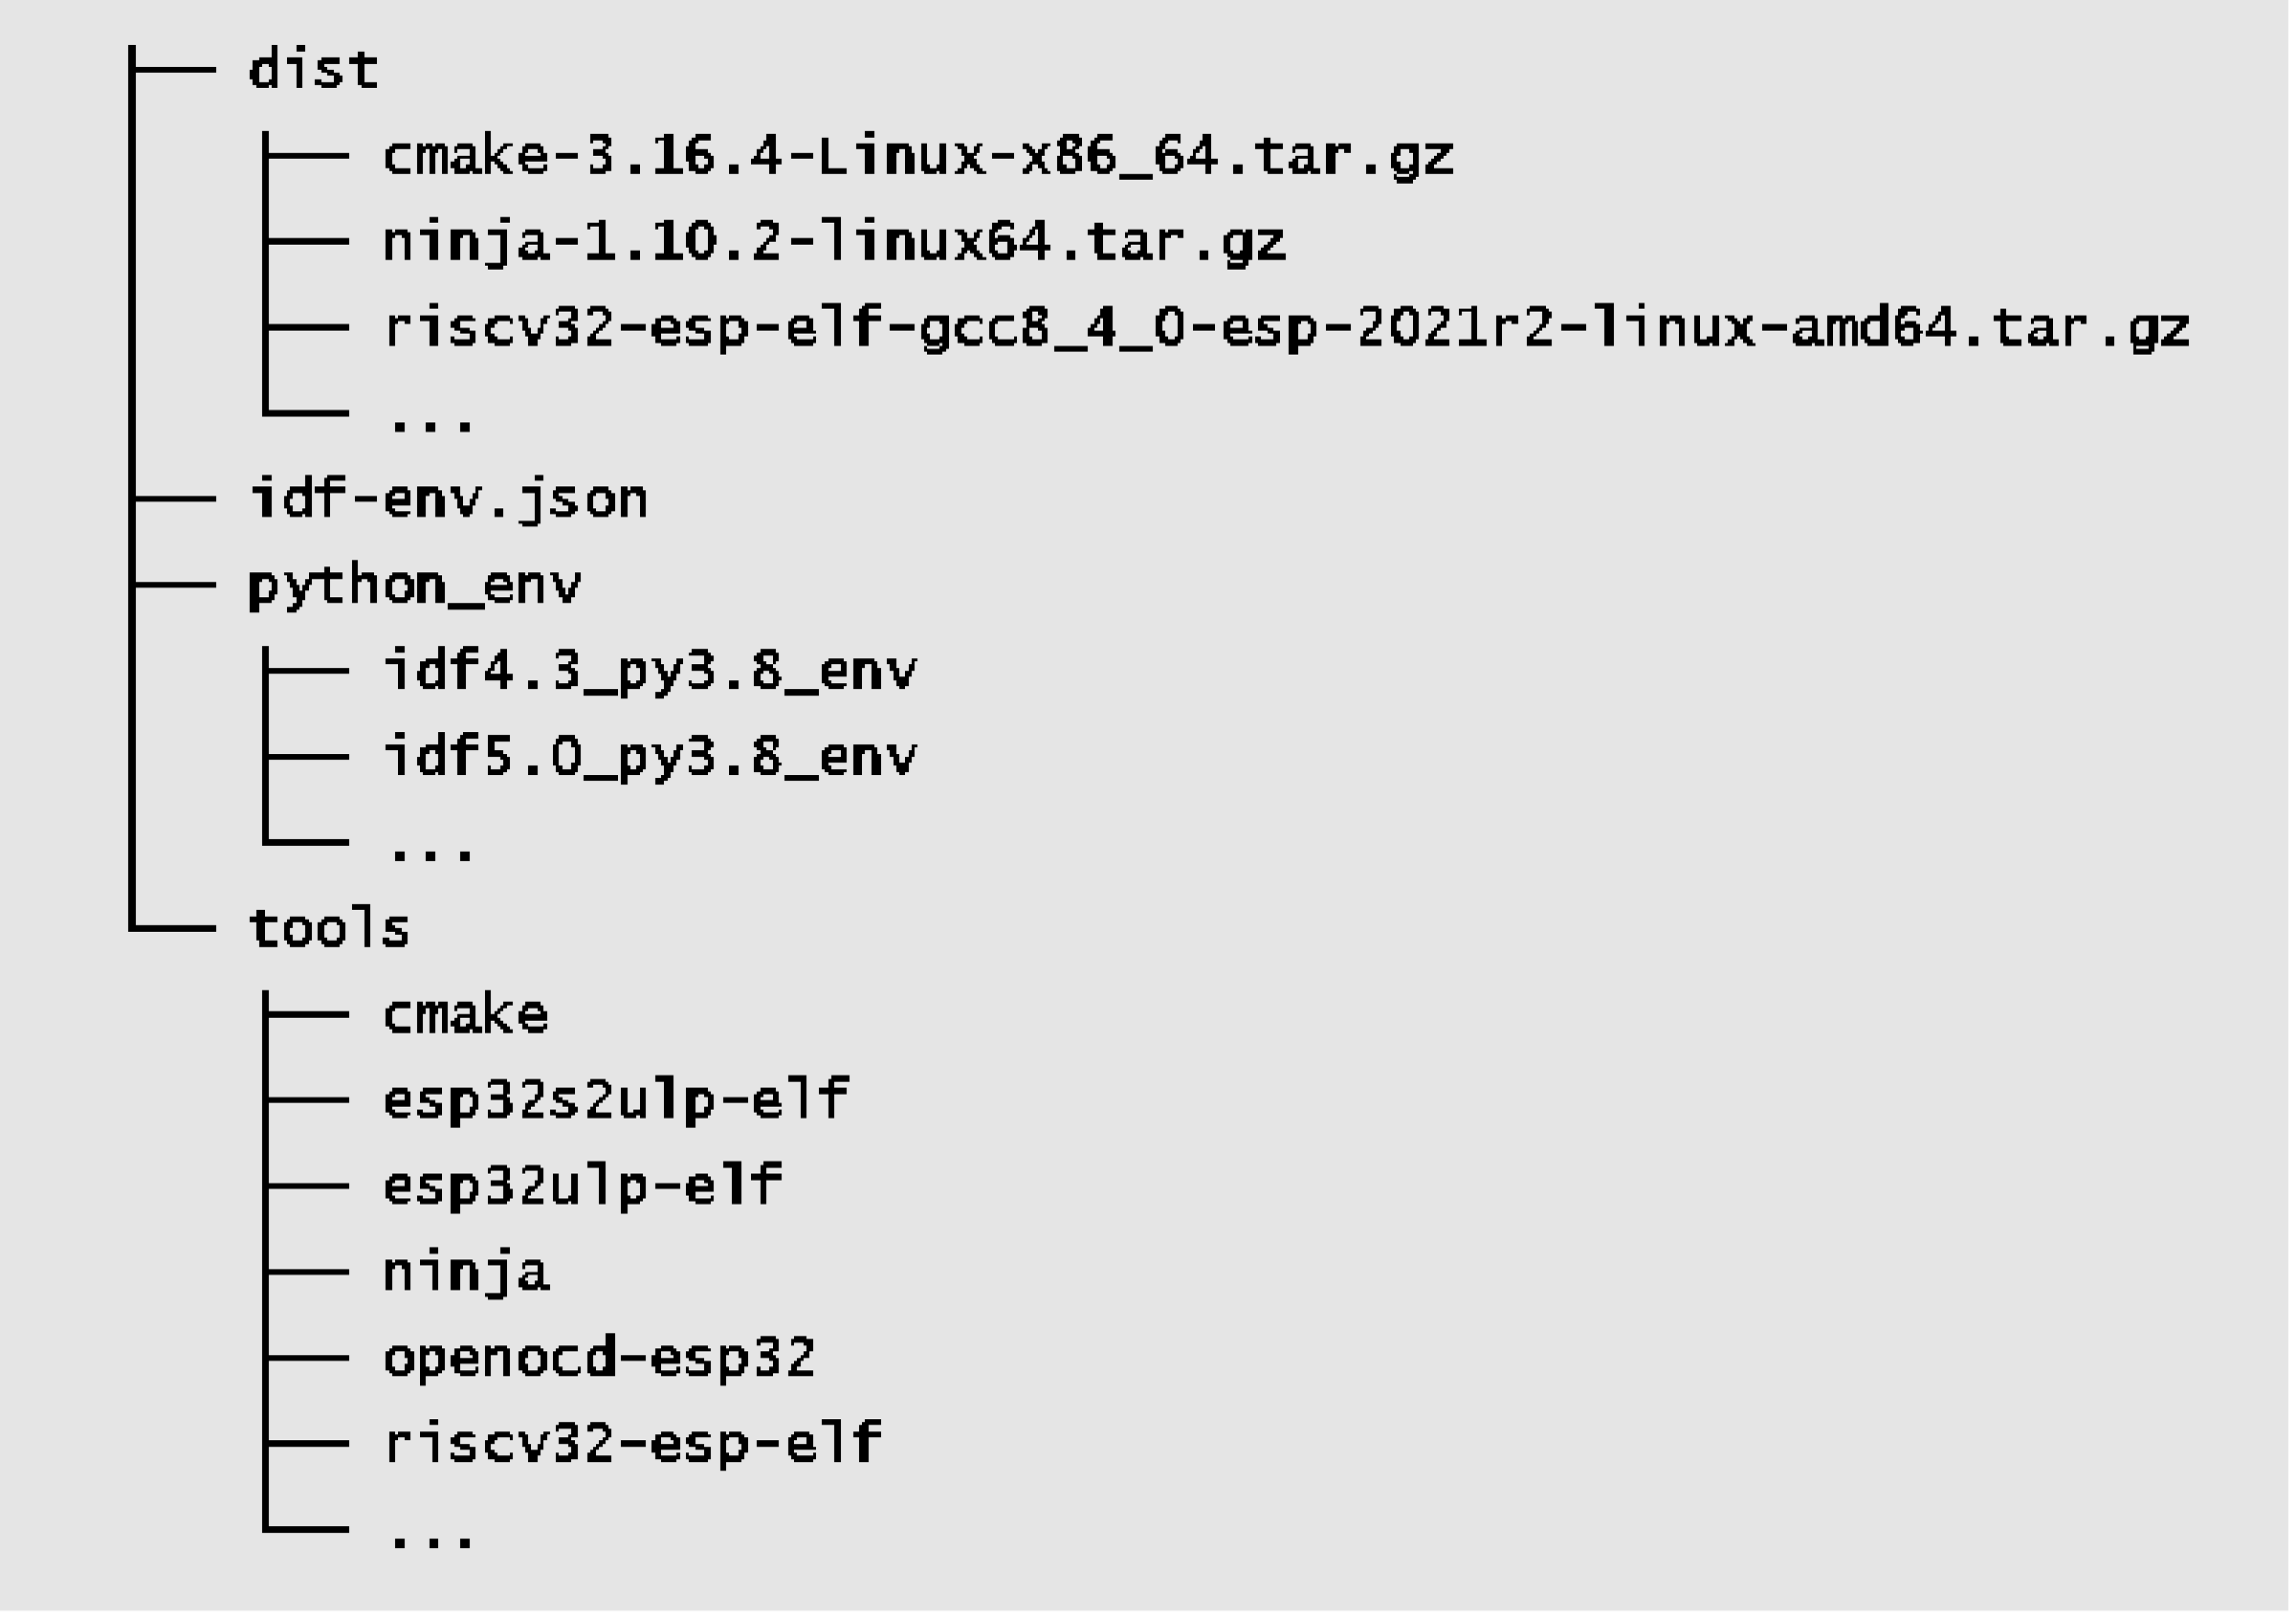
\includegraphics[width=0.75\textwidth]{D4Z/4-3}
        \caption{ESP-IDF compilation tool chain directory}
        \label{ESP-IDF compilation tool chain directory}
    \end{figure}

    \begin{enumerate}[label=\textbf{\alph*.},leftmargin=0em]
        \item \textbf{Software distribution directory \texttt{dist}}

        The ESP-IDF tool chain and other software are distributed in the form of compressed packages. During the installation process, the installation tool first downloads the compressed package to the \verb|dist| directory, and then extracts it to the specified directory. Once the installation is complete, the contents in this directory can be safely removed.

        \item \textbf{Python virtual environment directory \texttt{python\_env}}

        Different versions of ESP-IDF rely on specific versions of Python packages. Installing these packages directly on the same host can lead to conflicts between package versions. To address this, ESP-IDF utilises Python virtual environments to isolate different package versions. With this mechanism, developers can install multiple versions of ESP-IDF on the same host and easily switch between them by importing different environment variables.

        \item \textbf{ESP-IDF compilation tool chain directory \texttt{tools}}

        This directory mainly contains cross-compilation tools required to compile ESP-IDF projects, such as CMake tools, Ninja build tools, and the gcc tool chain that generates the final executable program. Additionally, this directory houses the standard library of the C/C++ language along with the corresponding header files. If a program references a system header file like \verb|#include <stdio.h>|, the compilation tool chain will locate the \verb|stdio.h| file within this directory.
    \end{enumerate}
\end{enumerate}

\section{Setting Up ESP-IDF Development Environment}
The ESP-IDF development environment supports mainstream operating systems such as Windows, Linux, and macOS. This section will introduce how to set up the development environment on each system. It is recommended to develop ESP32-C3 on Linux system, which will be introduced in detail here. Many instructions are applicable across platforms due to the similarity of the development tools. Therefore, it is advised to carefully read the content of this section.

\note{You can refer to the online documents available at
\url{https://bookc3.espressif.com/esp32c3}, which provide the commands mentioned in this section.}

\subsection{Setting up ESP-IDF Development Environment on Linux}
The GNU development and debugging tools required for the ESP-IDF development environment are native to the Linux system. Additionally, the command-line terminal in Linux is powerful and user-friendly, making it an ideal choice for ESP32-C3 development. You can select your preferred Linux distribution, but we recommend using Ubuntu or other Debian-based systems. This section provides guidance on setting up the ESP-IDF development environment on Ubuntu 20.04.

\subsubsection{1. Install required packages}
Open a new terminal and execute the following command to install all necessary packages. The command will automatically skip packages that are already installed.

\begin{codebloc}
\begin{tabular}{d}
\$ \textbf{sudo apt-get install git wget flex bison gperf python3 python3-pip python3- setuptools cmake ninja-build ccache libffi-dev libssl-dev dfu-util libusb-1.0-0}
\end{tabular}
\end{codebloc}

\note[TIPS]{You need to use the administrator account and password for the command above. By default, no information will be displayed when entering the password. Simply press the “Enter” key to continue the procedure.}

Git is a key code management tool in ESP-IDF. After successfully setting up the development environment, you can use the \verb|git log| command to view all code changes made since the creation of ESP-IDF. In addition, Git is also used in ESP-IDF to confirm version information, which is necessary for installing the correct tool chain corresponding to specific versions. Along with Git, other important system tools include Python. ESP-IDF incorporates numerous automation scripts written in Python. Tools such as CMake, Ninja-build, and Ccache are widely used in C/C++ projects and serve as the default code compilation and building tools in ESP-IDF. \verb|libusb-1.0-0| and \verb|dfu-util| are the main drivers used for USB serial communication and firmware burning.

Once the software packages are installed, you can use the \verb|apt show <package_name>| command to obtain detailed descriptions of each package. For example, use \verb|apt show git| to print the description information for the Git tool.

\note[Q: What to do if the Python version is not supported?]{\vspace{3pt}\leftskip 0em \textbf{A:} ESP-IDF v4.3 requires a Python version that is not lower than v3.6. For older versions of Ubuntu, please manually download and install a higher version of Python and set Python3 as the default Python environment. You can find detailed instructions by searching for the keyword \texttt{update-alternatives python}.}

\subsubsection{2. Download ESP-IDF repository code}
Open a terminal and create a folder named \verb|esp| in your home directory using the \verb|mkdir| command. You can choose a different name for the folder if you prefer. Use the \verb|cd| command to enter the folder.

\begin{codebloc}
\begin{tabular}{d}
\$ \textbf{mkdir -p $\sim$/esp}

\$ \textbf{cd $\sim$/esp}
\end{tabular}
\end{codebloc}

Use the \verb|git clone| command to download the ESP-IDF repository code, as shown below:

\begin{codebloc}
\begin{tabular}{d}
\$ \textbf{git clone -b v4.3.2 --recursive https://github.com/espressif/esp-idf.git}
\end{tabular}
\end{codebloc}

In the command above, the parameter \verb|-b v4.3.2| specifies the version to download (in this case, version 4.3.2). The parameter \verb|--recursive| ensures that all sub-repositories of ESP-IDF are downloaded recursively. Information about sub-repositories can be found in the \verb|.gitmodules| file.

\subsubsection{3. Install the ESP-IDF development tool chain}
Espressif provides an automated script \verb|install.sh| to download and install the tool chain. This script checks the current ESP-IDF version and operating system environment, and then downloads and installs appropriate version of Python tool packages and compilation tool chains. The default installation path for the tool chain is \texttt{$\sim$/.espressif}. All you need to do is to navigate to the \verb|esp-idf| directory and run \verb|install.sh|.

\begin{codebloc}
\begin{tabular}{d}
\$ \textbf{cd $\sim$/esp/esp-idf}

\$ \textbf{./install.sh}
\end{tabular}
\end{codebloc}

If you install the the tool chain successfully, the terminal will display:

\begin{codebloc}
\begin{tabular}{d}
All done!
\end{tabular}
\end{codebloc}

At this point, you have successfully set up the ESP-IDF development environment.

\subsection{Setting up ESP-IDF Development Environment on Windows}
\textbf{1. Download ESP-IDF tools installer}

\note[TIPS]{It is recommended to set up the ESP-IDF development environment on Windows 10 or above. You can download the installer from \url{https://dl.espressif.com/dl/esp-idf/}. The installer is also an open-source software, and its source code can be viewed at \url{https://github.com/espressif/idf-installer}.}

\begin{itemize}
    \item \textbf{Online ESP-IDF tools installer}
    
    This installer is relatively small, around 4 MB in size, and other packages and code will be downloaded during the installation process. The advantage of the online installer is that not only can software packages and code be downloaded on demand during the installation process, but also allows the installation of all available releases of ESP-IDF and the latest branch of GitHub code (such as the \verb|master| branch). The disadvantage is that it requires a network connection during the installation process, which may cause installation failure due to network problems.
    
    \item \textbf{Offline ESP-IDF tools installer}
    
    This installer is larger, about 1 GB in size, and contains all the software packages and code required for environment set up. The main advantage of the offline installer is that it can be used on computers without Internet access, and generally has a higher installation success rate. It should be noted that the offline installer can only install stable releases of ESP-IDF identified by v*.* or v*.*.*.
\end{itemize}

\textbf{2. Run the ESP-IDF tools installer}

After downloading a suitable version of the installer (take ESP-IDF Tools Offline 4.3.2 for example here), double-click the exe file to launch the ESP-IDF installation interface. The following demonstrates how to install ESP-IDF stable version v4.3.2 using the offline installer.

\begin{enumerate}[label=(\arabic*)]
    \item In the “Select installation language” interface shown in Figure \ref{“Select installation language” interface}, select the language to be used from the drop-down list.

    \begin{figure}[h!]
        \centering
        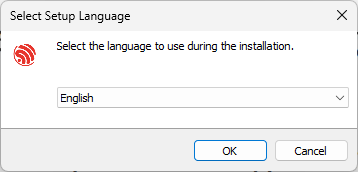
\includegraphics[width=0.41\textwidth]{D4Z/4-5}
        \caption{“Select installation language” interface}
        \label{“Select installation language” interface}
    \end{figure}

    \item After selecting the language, click “OK” to pop up the “License agreement” interface (see Figure \ref{“License agreement” interface}). After carefully reading the installation license agreement, select “I accept the agreement” and click “Next”.

    \begin{figure}[h!]
        \centering
        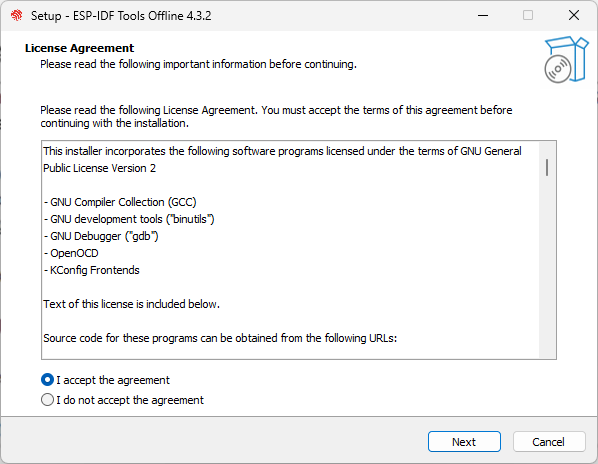
\includegraphics[width=0.53\textwidth]{D4Z/4-6}
        \caption{“License agreement” interface}
        \label{“License agreement” interface}
    \end{figure}

    \item Review the system configuration in the “Pre-installation system check” interface (see Figure \ref{“System check before installation” interface}). Check the Windows version and the installed antivirus software information. Click “Next” if all the configuration items are normal. Otherwise, you can click “Full log” for solutions based on key items.

    \begin{figure}[h!]
        \centering
        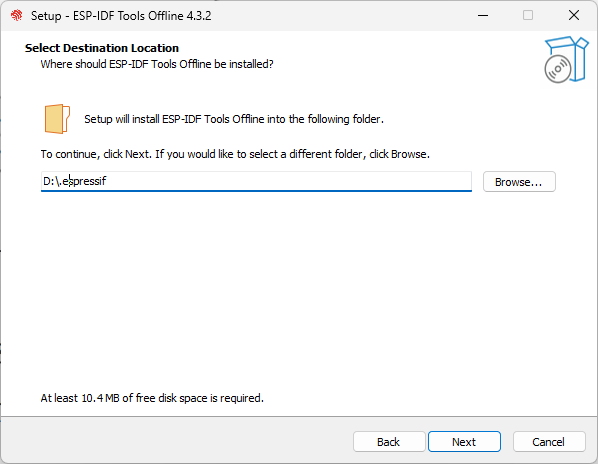
\includegraphics[width=0.53\textwidth]{D4Z/4-7}
        \caption{“System check before installation” interface}
        \label{“System check before installation” interface}
    \end{figure}

    \secnote[TIPS]{You can submit logs to \url{https://github.com/espressif/idf-installer/issues} for help.}

    \item Select the ESP-IDF installation directory. Here, select \verb|D:/.espressif|, as shown in Figure \ref{Select the ESP-IDF installation directory}, and click “Next”. Please note that \verb|.espressif| here is a hidden directory. After the installation is completed, you can view the specific contents of this directory by opening the file manager and displaying hidden items.

    \begin{figure}[h!]
        \centering
        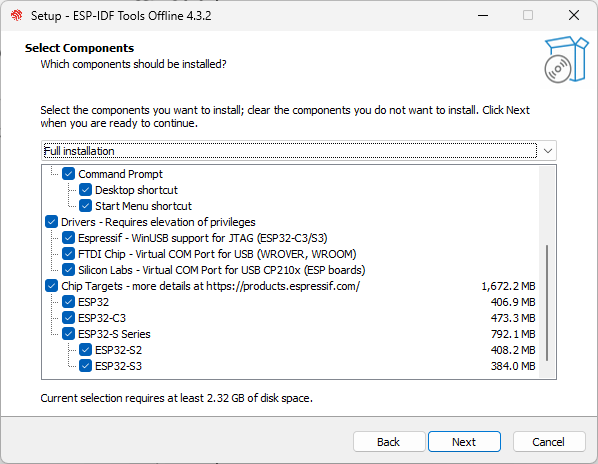
\includegraphics[width=0.53\textwidth]{D4Z/4-8}
        \caption{Select the ESP-IDF installation directory}
        \label{Select the ESP-IDF installation directory}
    \end{figure}

    \item Check the components that need to be installed, as shown in Figure \ref{Select the components to install}. It is recommended to use the default option, that is, complete installation, and then click “Next”.

    \begin{figure}[h!]
        \centering
        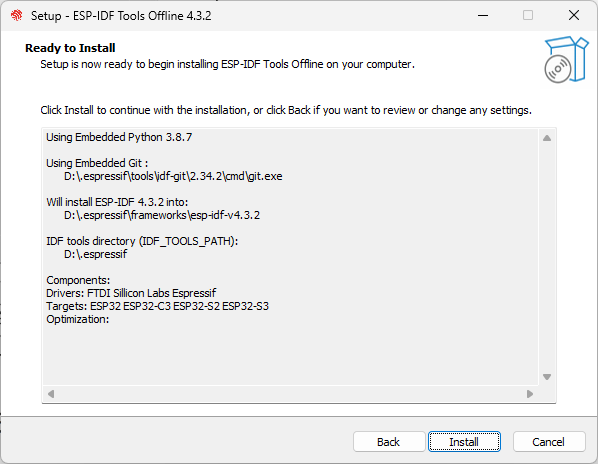
\includegraphics[width=0.55\textwidth]{D4Z/4-9}
        \caption{Select the components to install}
        \label{Select the components to install}
    \end{figure}

    \item Confirm the components to be installed and click “Install” to start the automated installation process, as shown in Figure \ref{Preparing for installation}. The installation process may last tens of minutes and the progress bar of the installation process is shown in Figure \ref{Installation progress bar}. Please wait patiently.

    \begin{figure}[h!]
        \centering
        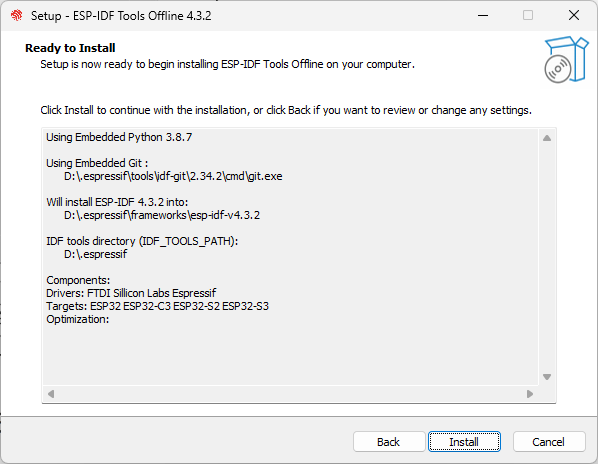
\includegraphics[width=0.55\textwidth]{D4Z/4-10}
        \caption{Preparing for installation}
        \label{Preparing for installation}
    \end{figure}

    \begin{figure}[h!]
        \centering
        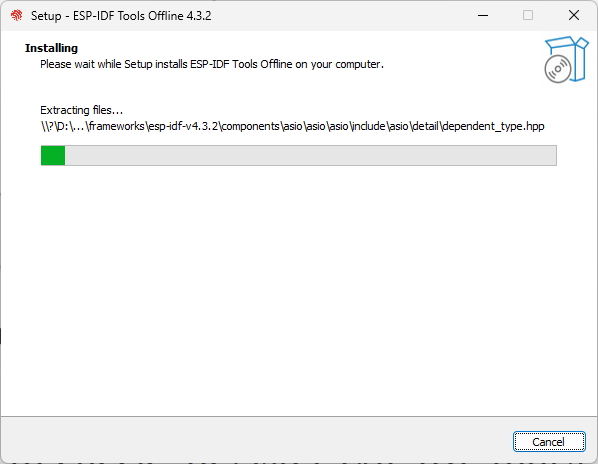
\includegraphics[width=0.55\textwidth]{D4Z/4-11}
        \caption{Installation progress bar}
        \label{Installation progress bar}
    \end{figure}

    \item After the installation is complete, it is recommended to check “Register the ESP-IDF Tools executables as Windows Defender exclusions...” to prevent antivirus software from deleting files. Adding exclusion items can also skip frequent scans by antivirus software, greatly improving the code compilation efficiency of the Windows system. Click “Finish” to complete the installation of the development environment, as shown in Figure \ref{Installation completed}. You can choose to check “Run ESP-IDF PowerShell environment” or “Run ESP-IDF command prompt”. Run the compilation window directly after installation to ensure that the development environment functions normally.

    \begin{figure}[h!]
        \centering
        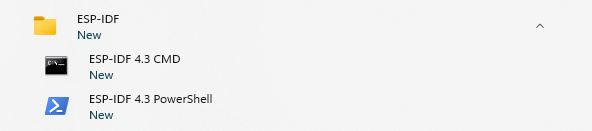
\includegraphics[width=0.55\textwidth]{D4Z/4-12}
        \caption{Installation completed}
        \label{Installation completed}
    \end{figure}

    \item Open the installed development environment in the program list (either ESP-IDF 4.3 CMD or ESP-IDF 4.3 PowerShell terminal, as shown in Figure \ref{Development environment installed}), and the ESP-IDF environment variable will be automatically added when running in the terminal. After that, you can use the \verb|idf.py| command for operations. The opened ESP-IDF 4.3 CMD is shown in Figure \ref{ESP-IDF 4.3 CMD}.

    \begin{figure}[h!]
        \centering
        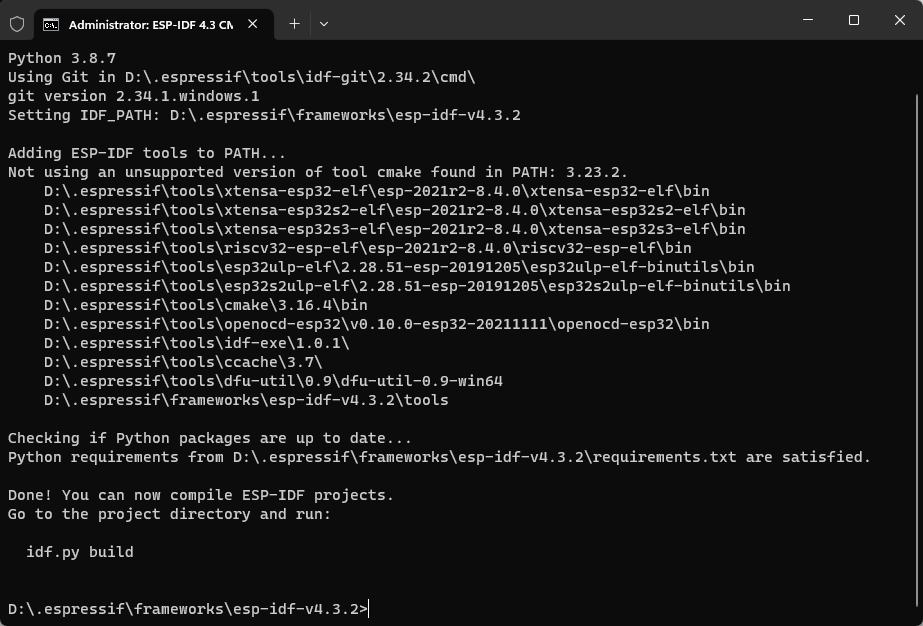
\includegraphics[width=0.4\textwidth,frame]{D4Z/4-13}
        \caption{Development environment installed}
        \label{Development environment installed}
    \end{figure}

    \begin{figure}[h!]
        \centering
        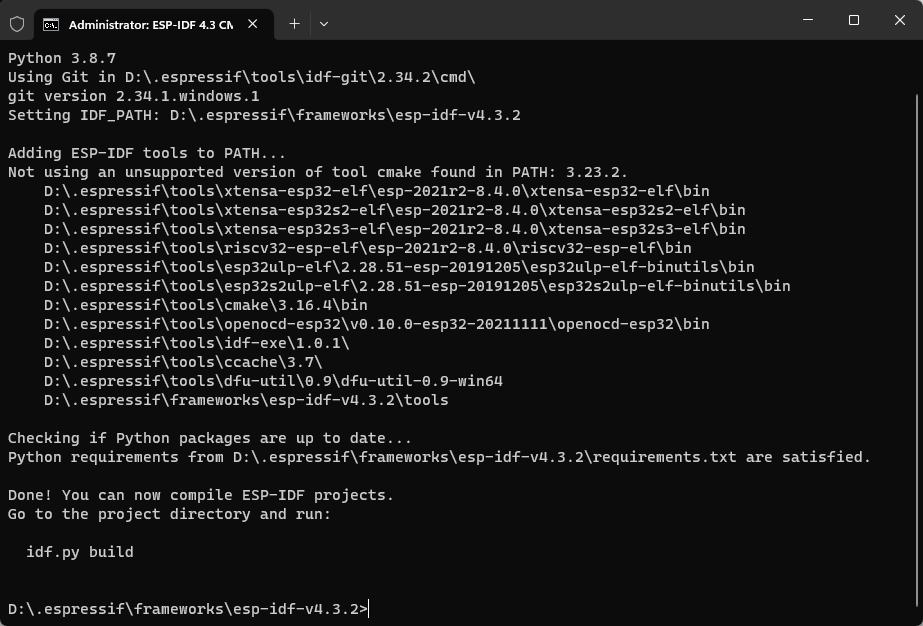
\includegraphics[width=0.55\textwidth]{D4Z/4-14}
        \caption{ESP-IDF 4.3 CMD}
        \label{ESP-IDF 4.3 CMD}
    \end{figure}
\end{enumerate}

\subsection{Setting up ESP-IDF Development Environment on Mac}
The process of installing the ESP-IDF development environment on a Mac system is the same as that on a Linux system. The commands for downloading the repository code and installing the tool chain are exactly the same. Only the commands for installing dependency packages are slightly different.

\textbf{1. Install dependency packages}

Open a terminal, and install pip, the Python package management tool, by running the following command:

\begin{codebloc}
\begin{tabular}{d}
\% \textbf{sudo easy\_install pip}
\end{tabular}
\end{codebloc}

Install Homebrew, a package management tool for macOS, by running the following command:

\begin{codebloc}
\begin{tabular}{d}
\% \textbf{/bin/bash -c "\$(curl -fsSL https://raw.githubusercontent.com/Homebrew/install/\newline HEAD/install.sh)"}
\end{tabular}
\end{codebloc}

Install the required dependency packages by running the following command:

\begin{codebloc}
\begin{tabular}{d}
\% \textbf{brew python3 install cmake ninja ccache dfu-util}
\end{tabular}
\end{codebloc}

\textbf{2. Download ESP-IDF repository code}

Follow the instructions provided in section 4.2.1 to download the ESP-IDF repository code. The steps are the same as for downloading on a Linux system.

\textbf{3. Install the ESP-IDF development tool chain}

Follow the instructions provided in section 4.2.1 to install the ESP-IDF development tool chain. The steps are the same as for installation on a Linux system.

\subsection{Installing VS Code}
By default, the ESP-IDF SDK does not include a code editing tool (though the latest ESP-IDF installer for Windows offers the option to install ESP-IDF Eclipse). You can use any text editing tool of your choice to edit the code and then compile it using terminal commands.

One popular code editing tool is VS Code (Visual Studio Code), which is a free and feature-rich code editor with a user-friendly interface. It offers various plugins that provide functionalities such as code navigation, syntax highlighting, Git version control, and terminal integration. Additionally, Espressif has developed a dedicated plugin called Espressif IDF for VS Code, which simplifies project configuration and debugging.

You can use the \verb|code| command in the terminal to quickly open the current folder in VS Code. Alternatively, you can use the shortcut \texttt{Ctrl+$\sim$} to open the system’s default terminal console within VS Code.

\note[TIPS]{It is recommended to use VS Code for ESP32-C3 code development. Download and install the latest version of VS Code at \url{https://code.visualstudio.com/}.}

\subsection{Introduction to Third-Party Development Environments}
In addition to the official ESP-IDF development environment, which primarily uses the C language, ESP32-C3 also supports other mainstream programming languages and a wide range of third-party development environments. Some notable options include:

\begin{term}{Arduino:}
    an open-source platform for both hardware and software, supporting various microcontrollers, including ESP32-C3.
    
    \vspace{6pt}
    It uses the C++ language and offers a simplified and standardised API, commonly referred to as the Arduino language. Arduino is widely used in prototype development and educational contexts. It provides an extensible software package and an IDE that allows for easy compilation and flashing.
\end{term}

\begin{term}{MicroPython:}
    a Python 3 language interpreter designed to run on embedded microcontroller platforms.
    
    \vspace{6pt}
    With a simple script language, it can directly access ESP32-C3’s peripheral resources (such as UART, SPI, and I2C) and communication functions (such as Wi-Fi and Bluetooth LE). This simplifies hardware interaction. MicroPython, combined with Python’s extensive mathematical operation library, enables the implementation of complex algorithms on ESP32-C3, facilitating the development of AI-related applications. As a script language, there is no need for repeated compilation; modifications can be made and scripts can be executed directly.
\end{term}

\begin{term}{NodeMCU:}
    an LUA language interpreter developed for ESP series chips.
    
    \vspace{6pt}
    It supports almost all peripheral functions of ESP chips and is lighter than MicroPython. Similar to MicroPython, NodeMCU uses a script language, eliminating the need for repeated compilation.
\end{term}

Furthermore, ESP32-C3 also supports the NuttX and Zephyr operating systems. NuttX is a real-time operating system that provides POSIX-compatible interfaces, enhancing application portability. Zephyr is a small real-time operating system specifically designed for IoT applications. It includes numerous software libraries required in IoT development, gradually evolving into a comprehensive software ecosystem.

This book does not provide detailed installation instructions for the aforementioned development environments. You can install a development environment based on your requirements by following the respective documentation and instructions.

\section{ESP-IDF Compilation System}
\subsection{Basic Concepts of Compilation System}
An ESP-IDF project is a collection of a main program with an entry function and multiple independent functional components. For example, a project that controls LED switches mainly consists of an entry program \verb|main| and a \verb|driver| component that controls GPIO. If you want to realise the LED remote control, you also need to add Wi-Fi, TCP/IP protocol stack, etc.

The compilation system can compile, link, and generate executable files (.bin) for the code through a set of building rules. The compilation system of ESP-IDF v4.0 and above versions is based on CMake by default, and the compilation script \verb|CMakeLists.txt| can be used to control the compilation behavior of the code. In addition to supporting the basic syntax of CMake, the ESP-IDF compilation system also defines a set of default compilation rules and CMake functions, and you can write the compilation script with simple statements.

\subsection{Project File Structure}
A project is a folder that contains an entry program \verb|main|, user-defined components, and files required to build executable applications, such as compilation scripts, configuration files, partition tables, etc. Projects can be copied and passed on, and the same executable file can be compiled and generated in machines with the same version of ESP-IDF development environment. A typical ESP-IDF project file structure is shown in Figure \ref{Typical ESP-IDF project file structure}.

\begin{figure}[h!]
    \centering
    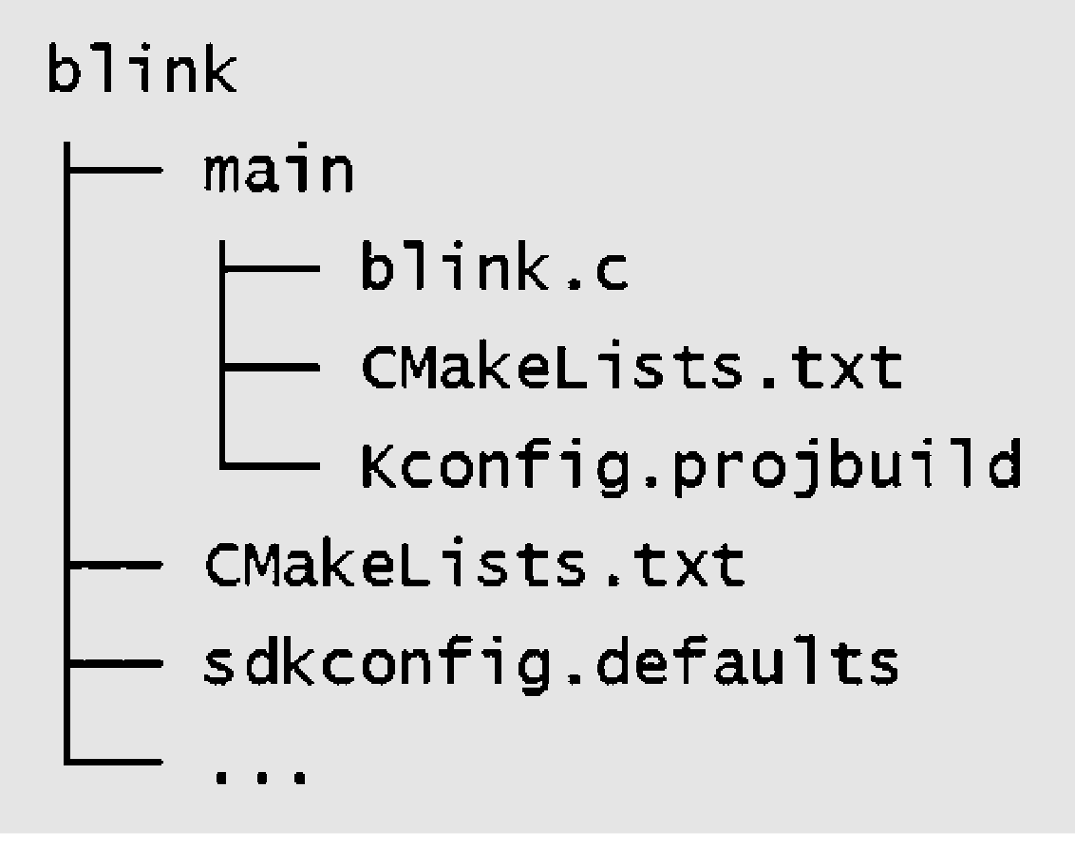
\includegraphics[width=0.35\textwidth]{D4Z/4-15}
    \caption{Typical ESP-IDF project file structure}
    \label{Typical ESP-IDF project file structure}
\end{figure}

Since ESP-IDF supports multiple IoT chips from Espressif, including ESP32, ESP32-S series, ESP32-C series, ESP32-H series, etc., a target needs to be determined before compiling the code. The target is both the hardware device that runs the application program and the build target of the compilation system.

Depending on your needs, you can specify one or more targets for your project. For example, through command \verb|idf.py set-target esp32c3|, you can set the compilation target to ESP32-C3, during which the default parameters and compilation tool chain path for ESP32-C3 will be loaded. After compilation, an executable program can be generated for ESP32-C3. You can also run the command \verb|set-target| again to set a different target, and the compilation system will automatically clean up and reconfigure.

\begin{term}{Components}
    Components in ESP-IDF are modular and independent code units managed within the compilation system. They are organised as folders, with the folder name representing the component name by default. Each component has its own compilation script that specifies its compilation parameters and dependencies. During the compilation process, components are compiled into separate static libraries (.a files) and eventually combined with other components to form the application program.

    \parskip 6pt
    ESP-IDF provides essential functions, such as the operating system, peripheral drivers, and network protocol stack, in the form of components. These components are stored in the \verb|components| directory located within the ESP-IDF root directory. Developers do not need to copy these components to the \verb|components| directory of \verb|myProject|. Instead, they only need to specify the dependency relationships of these components in the project’s \verb|CMakeLists.txt| file using the \verb|REQUIRES| or \verb|PRIV_REQUIRES| directives. The compilation system will automatically locate and compile the required components.

    Therefore, the \verb|components| directory under \verb|myProject| is not necessary. It is only used to include some custom components of the project, which can be third-party libraries or user-defined code. Additionally, components can be sourced from any directory other than ESP-IDF or the current project, such as from an open-source project saved in another directory. In this case, you only need to add the path of the component by setting the \verb|EXTRA_COMPONENT_DIRS| variable in the \verb|CMakeLists.txt| under the root directory. This directory will override any ESP-IDF component with the same name, ensuring the correct component is used.
\end{term}

\begin{term}{Entry program \texttt{main}}
    The \verb|main| directory within the project follows the same file structure as other components (e.g., \verb|component1|). However, it holds a special significance as it is a mandatory component that must exist in every project. The main directory contains the project’s source code and the user program’s entry point, typically named \verb|app_main|. By default, the execution of the user program starts from this entry point. The \verb|main| component also differs in that it automatically depends on all components within the search path. Therefore, there is no need to explicitly indicate dependencies using the \verb|REQUIRES| or \verb|PRIV_REQUIRES| directives in the \verb|CMakeLists.txt| file.
\end{term}

\begin{term}{Configuration file}
    The root directory of the project contains a configuration file called \verb|sdkconfig|, which contains the configuration parameters for all the components within the project. The \verb|sdkconfig| file is automatically generated by the compilation system and can be modified and regenerated by the command \verb|idf.py menuconfig|. The menuconfig options mainly originate from the \verb|Kconfig.projbuild| of the project and the \verb|Kconfig| of the components. Component developers generally add configuration items in \verb|Kconfig| to make the component flexible and configurable.
\end{term}

\begin{term}{\texttt{Build} directory}
    By default, the \verb|build| directory within the project stores intermediate files and the final executable programs generated by the \verb|idf.py build| command. In general, it is not necessary to directly access the contents of the \verb|build| directory. ESP-IDF provides predefined commands to interact with the directory, such as using the \verb|idf.py flash| command to automatically locate the compiled binary file and flash it to the specified flash address, or using the \verb|idf.py fullclean| command to clean the entire \verb|build| directory.
\end{term}

\begin{term}{Partition table (\texttt{partitions.csv})}
    Each project requires a partition table to divide the space of flash and specify the size and starting address of the executable program and user data space. Command \verb|idf.py |\\ \verb|flash| or OTA upgrade program will flash the firmware to the corresponding address according to this table. ESP-IDF provides several default partition tables in \verb|components/|\\ \verb|partition_table|, such as \verb|partitions_singleapp.csv| and \verb|partitions_two_|\\ \verb|ota.csv|, which can be selected in \verb|menuconfig|.
    
    \vspace{6pt}
    If the default partition table of the system cannot meet the requirements of the project, a custom \verb|partitions.csv| can be added to the project directory and be selected in \verb|menuconfig|.
\end{term}

\subsection{Default Build Rules of the Compilation System}
\begin{term}{Rules for overriding components with the same name}
    During the component search process, the compilation system follows a specific order. It first searches for internal components of ESP-IDF, then looks for components of the user project, and finally searches for components in \verb|EXTRA_COMPONENT_DIRS|. In cases where multiple directories contain components with the same name, the component found in the last directory will override any previous components with the same name. This rule allows for the customisation of ESP-IDF components within the user project, while keeping the original ESP-IDF code intact.
\end{term}

\begin{term}{Rules for including common components by default}
    As mentioned in section 4.3.2, components need to explicitly specify their dependencies on other components in the \verb|CMakeLists.txt|. However, common components such as \verb|freertos| are automatically included in the build system by default, even if their dependency relationships are not explicitly defined in the compilation script. ESP-IDF common components include \verb|freertos|, \verb|Newlib|, \verb|heap|, \verb|log|, \verb|soc|, \verb|esp_rom|, \verb|esp_common|, \verb|xtensa/riscv|, and \verb|cxx|. Using these common components avoids repetitive work when writing \verb|CMakeLists.txt| and make it more concise.
\end{term}

\begin{term}{Rules for overriding configuration items}
    Developers can add default configuration parameters by adding a default configuration file named \verb|sdkconfig.defaults| to the project. For example, adding \verb|CONFIG_LOG_|\\ \verb|DEFAULT_LEVEL_NONE = y| can configure the UART interface to not print log data by default. Furthermore, if specific parameters need to be set for a particular target, a configuration file named \verb|sdkconfig.defaults.TARGET_NAME| can be added, where \verb|TARGET_NAME| can be \verb|esp32s2|, \verb|esp32c3|, and so on. These configuration files are imported into the \verb|sdkconfig| during compilation, with the general default configuration file \verb|sdkconfig.defaults| being imported first, followed by the target-specific configuration file, such as \verb|sdkconfig.defaults.esp32c3|. In cases where there are configuration items with the same name, the latter configuration file will override the former.
\end{term}

\subsection{Introduction to the Compilation Script}
When developing a project using ESP-IDF, developers not only need to write source code but also need to write \verb|CMakeLists.txt| for the project and components. \verb|CMakeLists.txt| is a text file, also known as a compilation script, which defines a series of compilation objects, compilation configuration items, and commands to guide the compilation process of the source code. The compilation system of ESP-IDF v4.3.2 is based on CMake. In addition to supporting native CMake functions and commands, it also defines a series of custom functions, making it much easier to write compilation scripts.

The compilation scripts in ESP-IDF mainly include the project compilation script and the component compilation scripts. The \verb|CMakeLists.txt| in the root directory of the project is called the project compilation script, which guides the compilation process of the entire project. A basic project compilation script typically includes the following three lines:

\begin{codebloc}
\begin{tabular}{d}
\verb|1.  cmake_minimum_required(VERSION 3.5)|

\verb|2.  include($ENV{IDF_PATH}/tools/cmake/project.cmake)|

\verb|3.  project(myProject)|
\end{tabular}
\end{codebloc}

Among them, the \verb|cmake_minimum_required (VERSION 3.5)| must be placed on the first line, which is used to indicate the minimum CMake version number required by the project. Newer versions of CMake are generally backward compatible with older versions, so adjust the version number accordingly when using newer CMake commands to ensure compatibility.

\verb|include($ENV {IDF_PATH}/tools/cmake/project.cmake)| imports pre-defined\\ configuration items and commands of ESP-IDF compilation system, including the default build rules of the compilation system described in Section 4.3.3. \verb|project(myProject)| creates the project itself and specifies its name. This name will be used as the final output binary file name, i.e., \verb|myProject.elf| and \verb|myProject.bin|.

A project can have multiple components, including the \verb|main| component. The top-level directory of each component contains a \verb|CMakeLists.txt| file, which is called the component compilation script. Component compilation scripts are mainly used to specify component dependencies, configuration parameters, source code files, and included header files for compilation. With ESP-IDF’s custom function \verb|idf_component_register|, the minimum required code for a component compilation script is as follows:

\begin{codebloc}
\begin{tabular}{d}
\verb|1.  idf_component_register(SRCS "src1.c"|

\verb|2.                        INCLUDE_DIRS "include"|

\verb|3.                        REQUIRES component1)|
\end{tabular}
\end{codebloc}

The \verb|SRCS| parameter provides a list of source files in the component, separated by spaces if there are multiple files. The \verb|INCLUDE_DIRS| parameter provides a list of public header file directories for the component, which will be added to the \verb|include| search path for other components that depend on the current component. The \verb|REQUIRES| parameter identifies the public component dependencies for the current component. It is necessary for components to explicitly state which components they depend on, such as \verb|component2| depending on \verb|component1|. However, for the \verb|main| component, which depends on all components by default, the \verb|REQUIRES| parameter can be omitted.

In addition, native CMake commands can also be used in the compilation script. For example, use the command \verb|set| to set variables, such as \verb|set(VARIABLE "VALUE")|.

\subsection{Introduction to Common Commands}
ESP-IDF uses CMake (project configuration tool), Ninja (project building tool) and esptool (flash tool) in the process of code compilation. Each tool plays a different role in the compilation, building, and flash process, and also supports different operating commands. To facilitate user operation, ESP-IDF adds a unified front-end \verb|idf.py| that allows the above commands to be called quickly.

Before using \verb|idf.py|, make sure that:

\begin{itemize}[leftmargin=1.5em, noitemsep]
    \item The environment variable \verb|IDF_PATH| of ESP-IDF has been added to the current terminal.
    \item The command execution directory is the root directory of the project, which includes the project compilation script \verb|CMakeLists.txt|.
\end{itemize}

The common commands of \verb|idf.py| are as follows:

\begin{itemize}[leftmargin=1.5em, noitemsep]
    \item \verb|idf.py --help|: displaying a list of commands and their usage instructions.
    \item \verb|idf.py set-target <target>|: setting the compilation taidf.py fullcleanrget, such as replacing \verb|<target>| with \verb|esp32c3|.
    \item \verb|idf.py menuconfig|: launching \verb|menuconfig|, a terminal graphical configuration tool, which can select or modify configuration options, and the configuration results are saved in the \verb|sdkconfig| file.
    \item \verb|idf.py build|: initiating code compilation. The intermediate files and the final executable program generated by the compilation will be saved in the \verb|build| directory of the project by default. The compilation process is incremental, which means that if only one source file is modified, only the modified file will be compiled next time.
    \item \verb|idf.py clean|: cleaning the intermediate files generated by the project compilation. The entire project will be forced to compile in the next compilation. Note that the CMake configuration and the configuration modifications made by \verb|menuconfig| will not be deleted during cleanup.
    \item \verb|idf.py fullclean|: deleting the entire \verb|build| directory, including all CMake configuration output files. When building the project again, CMake will configure the project from scratch. Please note that this command will recursively delete all files in the build directory, so use it with caution, and the project configuration file will not be deleted.
    \item \verb|idf.py flash|: flashing the executable program binary file generated by \verb|build| to the target ESP32-C3. The options \verb|-p <port_name>| and \verb|-b <baud_rate>| are used to set the device name of the serial port and the baud rate for flashing, respectively. If these two options are not specified, the serial port will be automatically detected and the default baud rate will be used.
    \item \verb|idf.py monitor|: displaying the serial port output of the target ESP32-C3. The option \verb|-p| can be used to specify the device name of the host-side serial port. During serial port printing, press the key combination \verb|Ctrl+]| to exit the monitor.
\end{itemize}

The above commands can also be combined as needed. For example, the command \verb|idf.py |\\ \verb|build flash monitor| will perform code compilation, flash, and open the serial port monitor in sequence.

You can visit \url{https://bookc3.espressif.com/build-system} to know more about ESP-IDF compilation system.

\section{Practice: Compiling Example Program “Blink”}
\subsection{Example Analysis}
This section will take the program Blink as an example to analyse the file structure and coding rules of a real project in detail. The Blink program implements the LED blinking effect, and the project is located in the directory \verb|examples/get-started/blink|, which contains a source file, configuration files, and several compilation scripts.

The smart light project introduced in this book is based on this example program. Functions will be gradually added in later chapters to finally complete it.

\note[Source code]{In order to demonstrate the entire development process, the Blink program has been copied to \href{https://github.com/espressif/book-esp32c3-iot-projects/tree/main/device_firmware/1_blink}{\texttt{esp32c3-iot-projects/device\_firmware/1\_blink}}.}

The directory structure of the \verb|blink| project files is shown in Figure \ref{File directory structure of the blink project}.

\begin{figure}[h!]
    \centering
    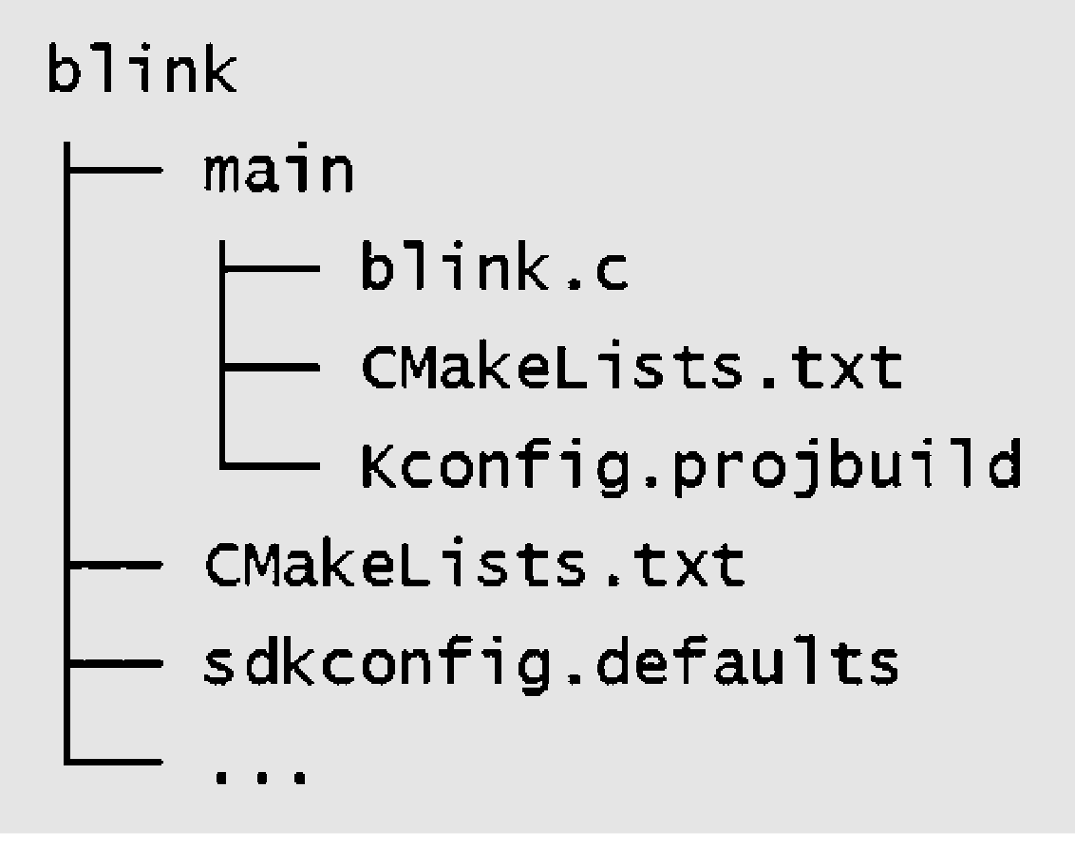
\includegraphics[width=0.3\textwidth]{D4Z/4-16}
    \caption{File directory structure of the \texttt{blink} project}
    \label{File directory structure of the blink project}
\end{figure}

The \verb|blink| project contains only one \verb|main| directory, which is a special component that must be included as described in section 4.3.2. The main directory is mainly used to store the implementation of the \verb|app_main()| function, which is the entry point to the user program.The \verb|blink| project does not include the \verb|components| directory, because this example only needs to use the components that come with ESP-IDF and does not require additional components. The \verb|CMakeLists.txt| included in the \verb|blink| project is used to guide the compilation process, while \verb|Kconfig.projbuild| is used to add configuration items for this example program in \verb|menuconfig|. Other unnecessary files will not affect the compilation of the code, so they will not be discussed here. A detailed introduction to the \verb|blink| project files is as follows.

\begin{codebloc}
\begin{tabular}{d}
\vspace{2pt}
\begin{verbatim}
1.  /*blink.c includes the following header files*/
2.  #include <stdio.h>              //Standard C library header file
3.  #include "freertos/freeRTOS.h"  //FreeRTOS main header file
4.  #include "freertos/task.h"      //FreeRTOS Task header file
5.  #include "sdkconfig.h"      //Configuration header file generated by kconfig
\end{verbatim}
\verb|6.  #include "driver/gpio.h"        //GPIO driver header file|
\end{tabular}
\end{codebloc}

The source file \verb|blink.c| contains a series of header files corresponding to function declarations. ESP-IDF generally follows the order of including standard library header files, FreeRTOS header files, driver header files, other component header files, and project header files. The order in which header files are included may affect the final compilation result, so try to follow the default rules. It should be noted that \verb|sdkconfig.h| is automatically generated by \verb|kconfig| and can only be configured through the command \verb|idf.py menuconfig|. Direct modification of this header file will be overwritten.

\begin{codebloc}
\begin{tabular}{d}
\vspace{2pt}
\begin{verbatim}
1.  /*You can select the GPIO corresponding to the LED in idf.py menuconfig,
    and the modification result of menuconfig is that the value of CONFIG_BLINK
    _GPIO will be changed. You can also directly modify the macro definition 
    here, and change CONFIG_BLINK_GPIO to a fixed value.*/
2.  #define BLINK_GPIO CONFIG_BLINK_GPIO
3.  void app_main(void)
4.  {
5.      /*Configure IO as the GPIO default function, enable pull-up mode, and
6.      disable input and output modes*/
\end{verbatim}
\verb|7.      gpio_reset_pin(BLINK_GPIO);|
\end{tabular}
\end{codebloc}

\begin{codebloc}
\begin{tabular}{d}
\vspace{2pt}
\begin{verbatim}
8.      /*Set GPIO to output mode*/
9.      gpio_set_direction(BLINK_GPIO, GPIO_MODE_OUTPUT);
10.     while(1) {
11.         /*Print log*/
12.         printf("Turning off the LED\n");
13.         /*Turn off the LED (output low level)*/
14.         gpio_set_level(BLINK_GPIO, 0);
15.         /*Delay (1000 ms)*/
16.         vTaskDelay(1000 / portTICK_PERIOD_MS);
17.         printf("Turning on the LED\n");
18.         /*Turn on the LED (output high level)*/
19.         gpio_set_level(BLINK_GPIO, 1);
20.         vTaskDelay(1000 / portTICK_PERIOD_MS);
21.     }
\end{verbatim}
\verb|22. }|
\end{tabular}
\end{codebloc}

The \verb|app_main()| function in the Blink example program serves as the entry point for user programs. It is a simple function with no parameters and no return value. This function is called after the system has completed initialisation, which includes tasks such as initialising the log serial port, configuring single/dual core, and configuring the watchdog.

The \verb|app_main()| function runs in the context of a task named \verb|main|. The stack size and priority of this task can be adjusted in \verb|menuconfig → Componentconfig → Common |\\ \verb|ESP-related|.

For simple tasks like blinking an LED, all the necessary code can be implemented directly in the \verb|app_main()| function. This typically involves initialising the GPIO corresponding to the LED and using a \verb|while(1)| loop to toggle the LED on and off. Alternatively, you can use FreeRTOS API to create a new task that handles the LED blinking. Once the new task is successfully created, you can exit the \verb|app_main()| function.

The content of \verb|main/CMakeLists.txt| file, which guides the compilation process for the main component, is as follows:

\begin{codebloc}
\begin{tabular}{d}
\verb|1.  idf_component_register(SRCS "blink.c" INCLUDE_DIRS "." )|
\end{tabular}
\end{codebloc}

Among them, \verb|main/CMakeLists.txt| only calls one compilation system function, that is \verb|idf_component_register|. Similar to the \verb|CMakeLists.txt| for most other components, \verb|blink.c| is added to \verb|SRCS|, and the source files added to \verb|SRCS| will be compiled. At the same time, “\verb|.|”, which represents the path where \verb|CMakeLists.txt| is located, should be added to \verb|INCLUDE_DIRS| as the search directories for header files. The content of \verb|CMakeLists.txt| is as follows:

\begin{codebloc}
\begin{tabular}{d}
\vspace{2pt}
\begin{verbatim}
1.  #Specify v3.5 as the oldest CMake version supported by the current project
2.  #Versions lower than v3.5 must be upgraded before compilation continues
3.  cmake_minimum_required(VERSION 3.5)
\end{verbatim}
\verb|4.  #Include the default CMake configuration of the ESP-IDF compilation system|
\end{tabular}
\end{codebloc}

\begin{codebloc}
\begin{tabular}{d}
\vspace{2pt}
\begin{verbatim}
5.  include($ENV{IDF_PATH}/tools/cmake/project.cmake)
6.  #Create a project named "blink"
\end{verbatim}
\verb|7.  project(myProject)|
\end{tabular}
\end{codebloc}

Among them, the \verb|CMakeLists.txt| in the root directory mainly includes \verb|$ENV{IDF_|\\ \verb|PATH}/tools/cmake/project.cmake|, which is the main CMake configuration file provided by ESP-IDF. It is used to configure the default rules of the ESP-IDF compilation system and define common functions such as \verb|idf_component_register|; \verb|project(blink)| creates a project called \verb|blink|, and the final firmware will be named \verb|blink.bin|.

\subsection{Compiling the Blink Program}
This section takes the Blink program as an example to demonstrate the compilation process of a simple ESP-IDF program. It is important to note that this section uses the high/low level of GPIO to drive the LED. However, the WS2812 indicator light requires a special communication protocol. You can refer to the example program in \href{https://github.com/espressif/esp-idf/tree/master/examples/peripherals/rmt/led_strip}{\texttt{esp-idf/examples/periphe-\\ rals/rmt/led\_strip}} for more information.

\subsubsection{1. Open a new terminal and import the ESP-IDF environment variables}
For Linux and Mac systems, use \texttt{cd $\sim$/esp/esp-idf} to navigate to the ESP-IDF folder. Then, import the ESP-IDF environment variables using the command \verb|. ./export.sh|. This process also performs a complete integrity check of the development environment.

\note[TIPS]{Please note that the \textbf{dot} before the space should not be omitted in \textbf{\texttt{. ./export.sh}}. The dot is equivalent to the \texttt{source} directive, which refers to executing the script and changing the environment variables in the current shell.}

\begin{figure}[h!]
    \Centering
    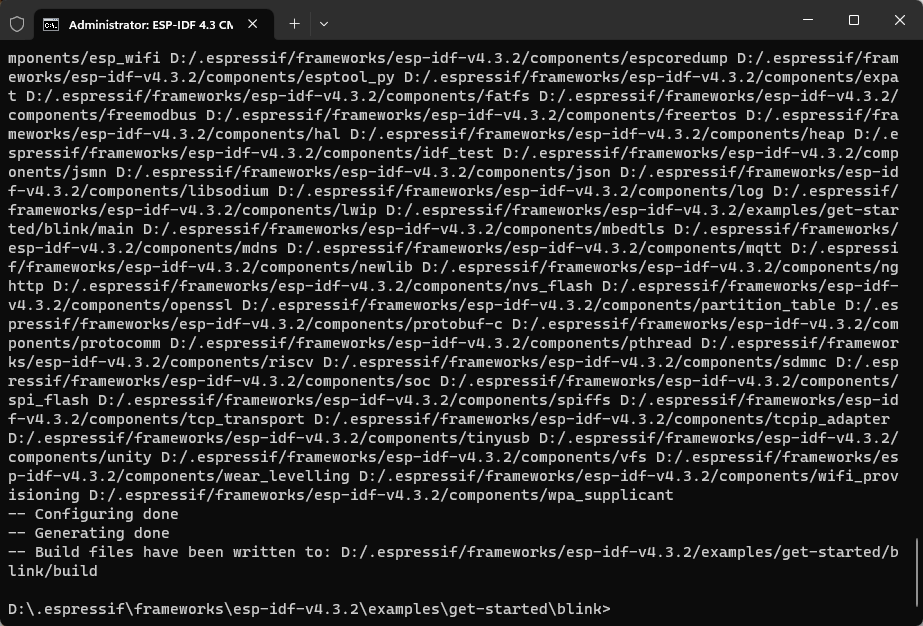
\includegraphics[width=0.6\textwidth]{D4Z/4-17}
    \caption{Automatic addition of environment variables in Windows system}
    \label{Automatic addition of environment variables in Windows system}
\end{figure}

For Windows systems, you can directly find and open ESP-IDF 4.3 CMD or ESP-IDF 4.3 PowerShell in the program list. After the terminal is opened, the environment variables will be automatically added, as shown in Figure \ref{Automatic addition of environment variables in Windows system}.

\subsubsection{2. Navigate to the root directory of the \texttt{blink} project}
Before compiling the project, navigate to the root directory of the project. To do this, use the command \verb|cd examples/get-started/blink|.

\subsubsection{3. Set the compilation target to ESP32-C3}
Use the command \verb|idf.py set-target esp32c3| to set the compilation target to ESP32-C3, as shown in Figure \ref{Set the compilation target to ESP32-C3}. If this step is skipped, the compilation target defaults to ESP32.

\begin{figure}[h!]
    \Centering
    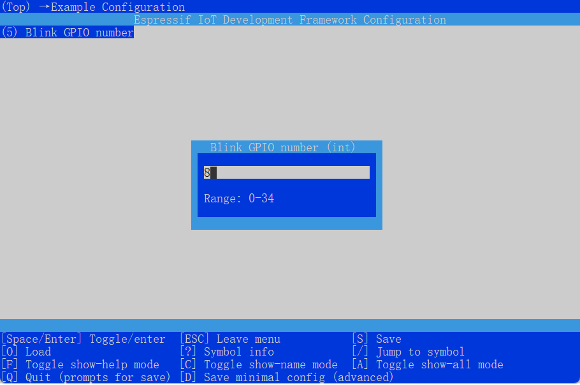
\includegraphics[width=0.63\textwidth]{D4Z/4-18}
    \caption{Set the compilation target to ESP32-C3}
    \label{Set the compilation target to ESP32-C3}
\end{figure}

\subsubsection{4. Configure GPIOs}
Use the command \verb|idf.py menuconfig| to enter the configuration interface. Navigate using the up/down keys and press Enter key to enter the \verb|Example Configuration|. Enter a number to change the GPIO to the specified pin, as shown in Figure 
\ref{Configure GPIO using menuconfig}. Save the configuration by following the prompts.

\begin{figure}[h!]
    \Centering
    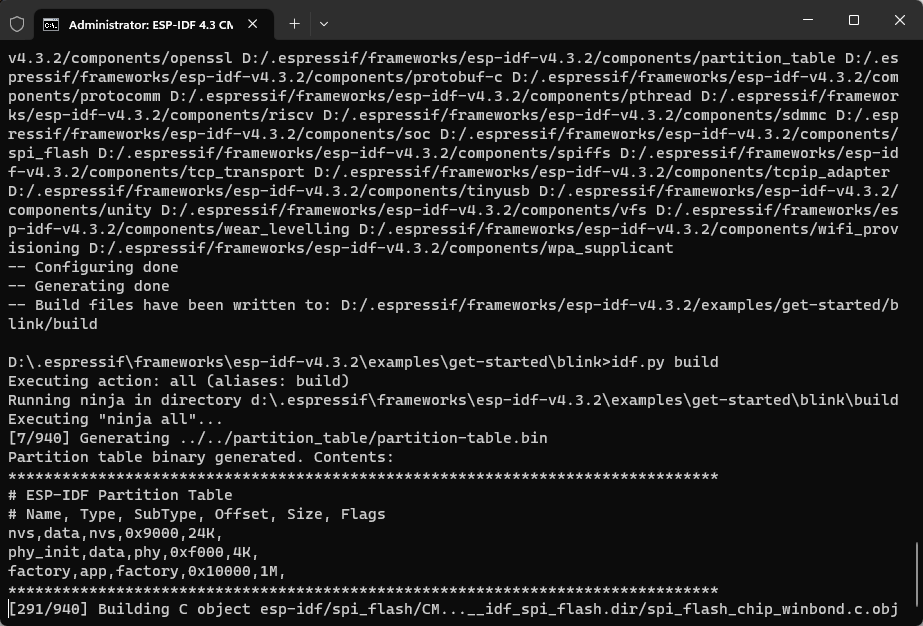
\includegraphics[width=0.55\textwidth]{D4Z/4-19}
    \caption{Configure GPIO using \texttt{menuconfig}}
    \label{Configure GPIO using menuconfig}
\end{figure}

\subsubsection{5. Build the code}
Use the command \verb|idf.py build| to build the code. The code building process is shown in Figure \ref{Code compilation process}. Relevant prompts and flash commands will be printed once the build is complete, as shown in Figure \ref{Prompt after code compilation is complete}.

\begin{figure}[h!]
    \Centering
    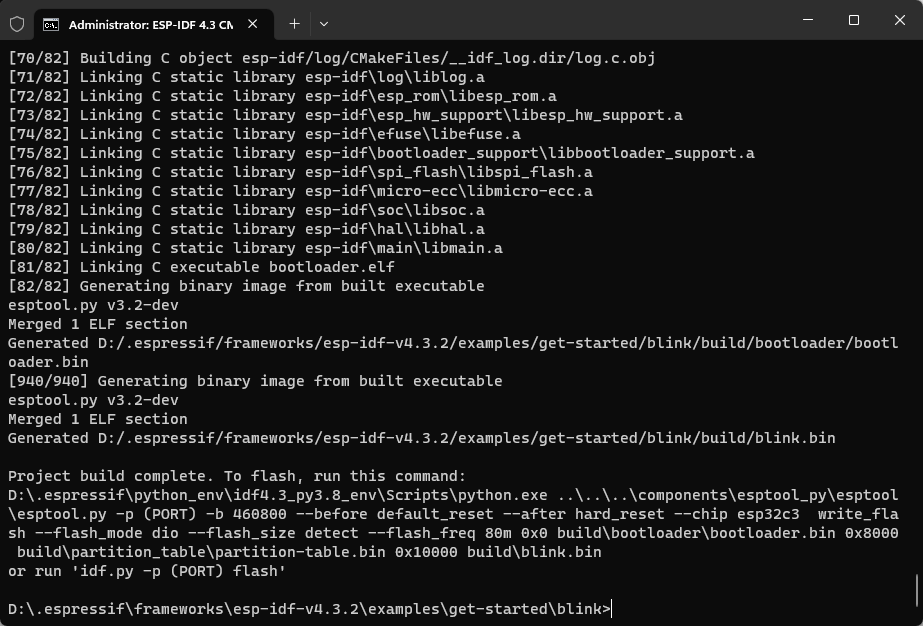
\includegraphics[width=0.55\textwidth]{D4Z/4-20}
    \caption{Code compilation process}
    \label{Code compilation process}
\end{figure}

\begin{figure}[h!]
    \Centering
    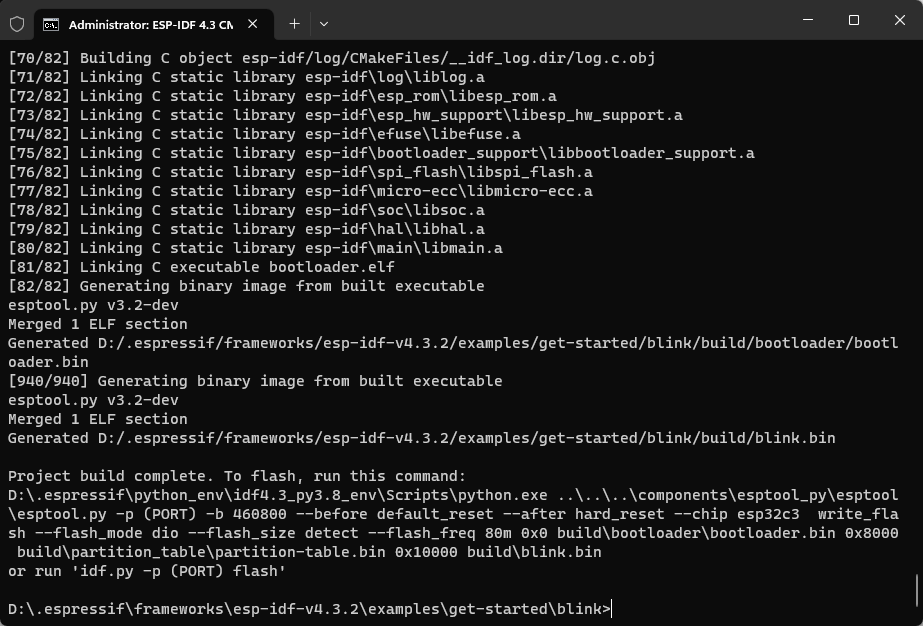
\includegraphics[width=0.55\textwidth]{D4Z/4-21}
    \caption{Prompt after code compilation is complete}
    \label{Prompt after code compilation is complete}
\end{figure}

\subsection{Flashing the Blink Program}
For Linux systems, connect the ESP32-C3 to the computer via USB-UART chip (such as CP2102), and use the command \verb|ls /dev/ttyUSB*| to view the serial port number. If the current serial port number printed is \verb|/dev/ttyUSB0|, use the command \verb|idf.py -p /dev|\\ \verb|/ttyUSB0 flash| to flash the program onto the ESP32-C3.

For Mac systems, connect the ESP32-C3 to the computer via USB-UART chip (such as CP2102), and use the command \verb|ls /dev/cu.*| to view the serial port number. If the current serial port number printed is \verb|/dev/cu.SLAB_USBtoUART|, use the command \verb|idf.py |\\ \verb|-p /dev/cu.SLAB_USBtoUART flash| to flash the program onto the ESP32-C3.

For Windows systems, connect the ESP32-C3 to the computer via USB-UART chip (such as CP2102), and view the serial port number through the device manager. If the current serial port number is \verb|COM5|, use the command \verb|idf.py -p COM5 flash| to flash the program onto the ESP32-C3.

After the flashing process is completed, you will see a prompt as shown in Figure \ref{Prompt in the console after flashing is completed} in the console. When the following log appears, the code will start executing, and the LED on the development board will start flashing.

\begin{codebloc}
\begin{tabular}{d}
Hard resetting via RTS pin...

Done
\end{tabular}
\end{codebloc}

\begin{figure}[h!]
    \Centering
    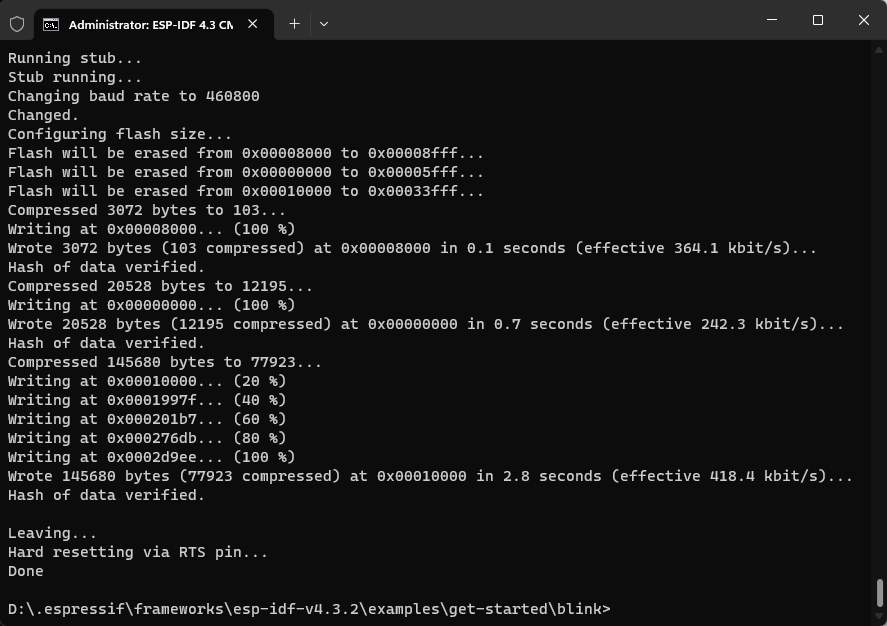
\includegraphics[width=0.7\textwidth]{D4Z/4-22}
    \caption{Prompt in the console after flashing is completed}
    \label{Prompt in the console after flashing is completed}
\end{figure}

\subsection{Serial Port Log Analysis of the Blink Program}
Once the firmware compilation and download are completed, navigate to the project folder, and run the command \verb|idf.py monitor|. This will open a monitor with coloured font. The monitor will output the serial port log of the target ESP32-C3. The content is divided into three parts by default: \textbf{first-level bootloader information}, \textbf{second-level bootloader information}, and \textbf{user program output}. During the output of log, you can press the \verb|Ctrl+]| key combination to exit the log output.

\begin{codebloc}
\begin{tabular}{d}
\vspace{2pt}
\begin{verbatim}
ESP-ROM:esp32c3-api1-20210207
Build:Feb  7 2021
rst:0x1 (POWERON),boot:0xc (SPI_FAST_FLASH_BOOT)
SPIWP:0xee
mode:DIO, clock div:1
load:0x3fcd6100,len:0x1798
load:0x403ce000,len:0x8dc
load:0x403d0000,len:0x2984
\end{verbatim}
\verb|entry 0x403ce000|
\end{tabular}
\end{codebloc}

\subsubsection{First-level bootloader information}
By default, the first-level bootloader information is output from UART and cannot be turned off through configuration in ESP-IDF version 4.3.2. This information includes the ROM code version information fixed internally in the chip. Different chips in the same series may have different ROM code versions due to ROM repairs and feature expansions. It also includes the reason for the chip restart, such as \verb|rst:0x1| indicating power-on restart of the chip, \verb|rst:0x3| indicating software-triggered restart, \verb|rst:0x4| indicating software exception restart, etc. You can use this information to assess the status of the chip. Additionally, it provides details about the chip’s boot mode, such as \verb|boot:0xc| indicating SPI Flash Boot mode (normal operation mode, in which the code in flash is loaded and executed), and \verb|boot:0x4| indicating Flash Download mode, in which the content of flash can be erased and programmed.

\subsubsection{Second-level bootloader information}
The output of second-level bootloader information can be disabled by setting \verb|menuconfig|\\ \verb|(Top) → Bootloader config → Bootloader log verbosity| to \verb|No output|.

This information mainly includes the ESP-IDF version, flash operating mode and speed, system partition and stack allocation, as well as the application name and version.

\begin{codebloc}
\begin{tabular}{d}
\vspace{2pt}
\begin{verbatim}
I (30) boot: ESP-IDF v4.3.2-1-g887e7c0c73-dirty 2nd stage bootloader
I (30) boot: compile time 18:27:35
I (30) boot: chip revision: 3
\end{verbatim}
\verb|I (34) boot.esp32c3: SPI Speed      : 80MHz|
\end{tabular}
\end{codebloc}

\begin{codebloc}
\begin{tabular}{d}
\vspace{2pt}
\begin{verbatim}
I (38) boot.esp32c3: SPI Mode       : DIO
I (43) boot.esp32c3: SPI Flash Size : 2MB
I (48) boot: Enabling RNG early entropy source...
I (53) boot: Partition Table:
I (57) boot: ## Label           Usage           Type ST Offset   Length
I (64) boot:  0 nvs             WiFi data       01 02 00009000 00006000
I (72) boot:  1 phy_init        RF data         01 01 0000f000 00001000
I (79) boot:  2 factory         factory app     00 00 00010000 00100000
I (86) boot: End of partition table
\end{verbatim}
\fontsize{9.5pt}{10pt}\selectfont
\begin{verbatim}
I (91) esp_image: segment 0: paddr=00010020 vaddr=3c020020 size=06058h (24664) map
I (103) esp_image: segment 1: paddr=00016080 vaddr=3fc89c00 size=01a88h (6792) load
I (109) esp_image: segment 2: paddr=00017b10 vaddr=40380000 size=08508h (34056) load
I (122) esp_image: segment 3: paddr=00020020 vaddr=42000020 size=15c54h (89172) map
I (138) esp_image: segment 4: paddr=00035c7c vaddr=40388508 size=0157ch (5500) load
I (139) esp_image: segment 5: paddr=00037200 vaddr=50000000 size=00010h (16) load
\end{verbatim}
\footnotesize
\begin{verbatim}
I (147) boot: Loaded app from partition at offset 0x10000
I (150) boot: Disabling RNG early entropy source...
I (166) cpu_start: Pro cpu up.
I (179) cpu_start: Pro cpu start user code
I (179) cpu_start: cpu freq: 160000000
I (179) cpu_start: Application information:
I (182) cpu_start: Project name:   blink
I (186) cpu_start: App version:    v4.3.2-1-g887e7c0c73-dirty
I (193) cpu_start: Compile time:   Jan 26 2022 18:27:31
I (199) cpu_start: ELF file SHA256:  dadcae8e7bb964ab...
I (205) cpu_start: ESP-IDF:         v4.3.2-1-g887e7c0c73-dirty
I (212) heap_init: Initializing. RAM available for dynamic allocation:
I (219) heap_init: At 3FC8C4D0 len 00033B30 (206 KiB): DRAM
I (225) heap_init: At 3FCC0000 len 0001F060 (124 KiB): STACK/DRAM
I (232) heap_init: At 50000010 len 00001FF0 (7 KiB): RTCRAM
I (238) spi_flash: detected chip: generic
I (243) spi_flash: flash io: dio
W (247) spi_flash: Detected size(4096k) larger than the size in the binary image 
header(2048k). Using the size in the binary image header.
I (260) sleep: Configure to isolate all GPIO pins in sleep state
I (267) sleep: Enable automatic switching of GPIO sleep configuration
\end{verbatim}
\verb|I (274) cpu_start: Starting scheduler.|
\end{tabular}
\end{codebloc}

\subsubsection{User program output}
The user program output includes all information that is printed using the \verb|printf()| function, which is the standard output function in the C language, or the \verb|ESP_LOG()| function, which is a custom output function provided by ESP-IDF. It is recommended to use \verb|ESP_LOG()| because it allows you to specify the log level for better organisation and filtering of logs.

You can configure which logs above a certain level are output through \verb|menuconfig(Top) |\\ \verb|→ Component config → Log output|. This allows you to control the verbosity of the logs and customise the level of detail that is displayed during runtime.

\begin{codebloc}
\begin{tabular}{d}
\vspace{2pt}
\begin{verbatim}
I (278) gpio: GPIO[5]| InputEn: 0| OutfgputEn: 0| OpenDrain: 0| Pullup: 1| 
Pulldown: 0| Intr:0 
Turning off the LED
Turning on the LED
Turning off the LED
\end{verbatim}
\verb|Turning on the LED|
\end{tabular}
\end{codebloc}

In addition to log output, \verb|idf.py monitor| can also parse system exceptions and trace software errors. For example, when the application crashes, the following register dump and traceback information will be generated:

\begin{codebloc}
\begin{tabular}{d}
\vspace{2pt}
\begin{verbatim}
Guru Meditation Error of type StoreProhibited occurred on core 0. Exception was 
unhandled.
Register dump:
PC  : 0x400f360d  PS    : 0x00060330  A0    : 0x800dbf56  A1    : 0x3ffb7e00
A2  : 0x3ffb136c  A3    : 0x00000005  A4    : 0x00000000  A5    : 0x00000000
A6  : 0x00000000  A7    : 0x00000080  A8    : 0x00000000  A9    : 0x3ffb7dd0
A10 : 0x00000003  A11   : 0x00060f23  A12   : 0x00060f20  A13   : 0x3ffba6d0
A14 : 0x00000047  A15   : 0x0000000f  SAR   : 0x00000019  EXCCAUSE  : 0x0000001d
EXCVADDR: 0x00000000  LBEG : 0x4000c46c  LEND : 0x4000c477  LCOUNT  : 0x00000000

Backtrace: 0x400f360d:0x3ffb7e00 0x400dbf56:0x3ffb7e20 0x400dbf5e:0x3ffb7e40 
\end{verbatim}
\verb|0x400dbf82:0x3ffb7e60 0x400d071d:0x3ffb7e90|
\end{tabular}
\end{codebloc}

Based on the register address, the IDF monitor will query the compiled \verb|ELF| file and trace the code call process when the application crashes, outputting the function call information to the monitor:

\begin{codebloc}
\begin{tabular}{d}
\vspace{2pt}
\begin{verbatim}
Guru Meditation Error of type StoreProhibited occurred on core 0. Exception was 
unhandled.
Register dump:
PC  : 0x400f360d  PS    : 0x00060330  A0    : 0x800dbf56  A1    : 0x3ffb7e00
0x400f360d: do_something_to_crash at /home/gus/esp/32/idf/examples/get-started/
hello_world/main/./hello_world_main.c:57
(inlined by) inner_dont_crash at /home/gus/esp/32/idf/examples/get-started/hello
_world/main/./hello_world_main.c:52
A2  : 0x3ffb136c  A3    : 0x00000005  A4    : 0x00000000  A5    : 0x00000000
A6  : 0x00000000  A7    : 0x00000080  A8    : 0x00000000  A9    : 0x3ffb7dd0
A10 : 0x00000003  A11   : 0x00060f23  A12   : 0x00060f20  A13   : 0x3ffba6d0
A14 : 0x00000047  A15   : 0x0000000f  SAR   : 0x00000019  EXCCAUSE  : 0x0000001d
EXCVADDR: 0x00000000  LBEG : 0x4000c46c  LEND : 0x4000c477  LCOUNT  : 0x00000000

Backtrace: 0x400f360d:0x3ffb7e00 0x400dbf56:0x3ffb7e20 0x400dbf5e:0x3ffb7e40 
0x400dbf82:0x3ffb7e60 0x400d071d:0x3ffb7e90
0x400f360d: do_something_to_crash at /home/gus/esp/32/idf/examples/get-started/ 
\end{verbatim}
\verb|hello_world/main/./hello_world_main.c:57|
\end{tabular}
\end{codebloc}

\begin{codebloc}
\begin{tabular}{d}
\vspace{2pt}
\begin{verbatim}
(inlined by) inner_dont_crash at /home/gus/esp/32/idf/examples/get-started/hello
_world/main/./hello_world_main.c:52
0x400dbf56: still_dont_crash at /home/gus/esp/32/idf/examples/get-started/hello
_world/main/./hello_world_main.c:47
0x400dbf5e: dont_crash at /home/gus/esp/32/idf/examples/get-started/hello_world/
main/./hello_world_main.c:42
0x400dbf82: app_main at /home/gus/esp/32/idf/examples/get-started/hello_world/
main/./hello_world_main.c:33
\end{verbatim}
\verb|0x400d071d: main_task at /home/gus/esp/32/idf/components/esp32/./cpu_start.c:254|
\end{tabular}
\end{codebloc}

The trace information of the monitor shows that the application crashes in the function \verb|do_something_to_crash()|, which is called by the function \verb|app_main() → dont_|\\ \verb|crash() → still_dont_crash() → inner_dont_crash() → do_something|\\ \verb|_to_crash()|. Based on this, the input/output parameters of each link can be checked to determine the cause of the crash.

\section{Summary}
In this chapter, we have covered the setup of the official software development environment, ESP-IDF, for ESP32-C3. We have introduced the code resources and file structure of ESP-IDF and provided a demonstration of the ESP-IDF project structure, compilation system, and related development tools using a simple example.

By following the instructions in this chapter, you can start developing with ESP-IDF for simple projects. However, for more specific and advanced compilation requirements, it is recommended to refer to both the ESP-IDF official documentation and the CMake official documentation.

{\makeatletter
\let\ps@plain\ps@empty
\makeatother
\part[Hardware and Driver Development]{\partpic{Starting/2c}}
}

\chapter[Hardware Design of Smart Light Products based on ESP32-C3]{\chaptertitle{Hardware Design of Smart Light Products based on ESP32-C3}{Hardware Design of Smart Light Products based on ESP32-C3}}

\vspace{36pt}
In this chapter, we will first introduce the main components of smart light products and their application scenarios, and take LED smart lights as an example to demonstrate their major hardware blocks. Then, we will use ESP32-C3 chips and modules to design a smart light product capable of dimming, colour changing, and wireless communication. The design provided in this chapter can also be extended and applied to various LED products such as light strips, ceiling lights, spotlights, etc.

\section{Features and Composition of Smart Light Products}
Smart light products generally use LEDs as light sources. LEDs are solid-state light sources and semiconductor light devices, characterised by low power consumption and long lifespan, easy to control, and pollution-free. Compared with traditional lighting products, they have higher efficiency of light energy conversion. At the same time, smart light products have wireless connectivity functionality, supporting connection to wireless routers or smart gateways through Wi-Fi, Bluetooth LE, or ZigBee, and then connection to the Internet or cloud servers. You can not only use smartphones, tablets, smart speakers that support voice control, and smart control panels to adjust their brightness and colour, as well as setting timers for turning on/off the lights. You can also group multiple lights together and control their brightness and colour in batch. You can pre-set lighting scenes for different occasions, such as “theatre mode” for dimming the ambient lighting, “reading mode” for a soft and eye-friendly brightness, “music mode” for colour changing and light blinking following the beat of the music, and “sleep mode” for turning off all the lights except the night lamp. The structure of a smart light system is shown in Figure 5.1.

\begin{figure}[h!]
    \centering
    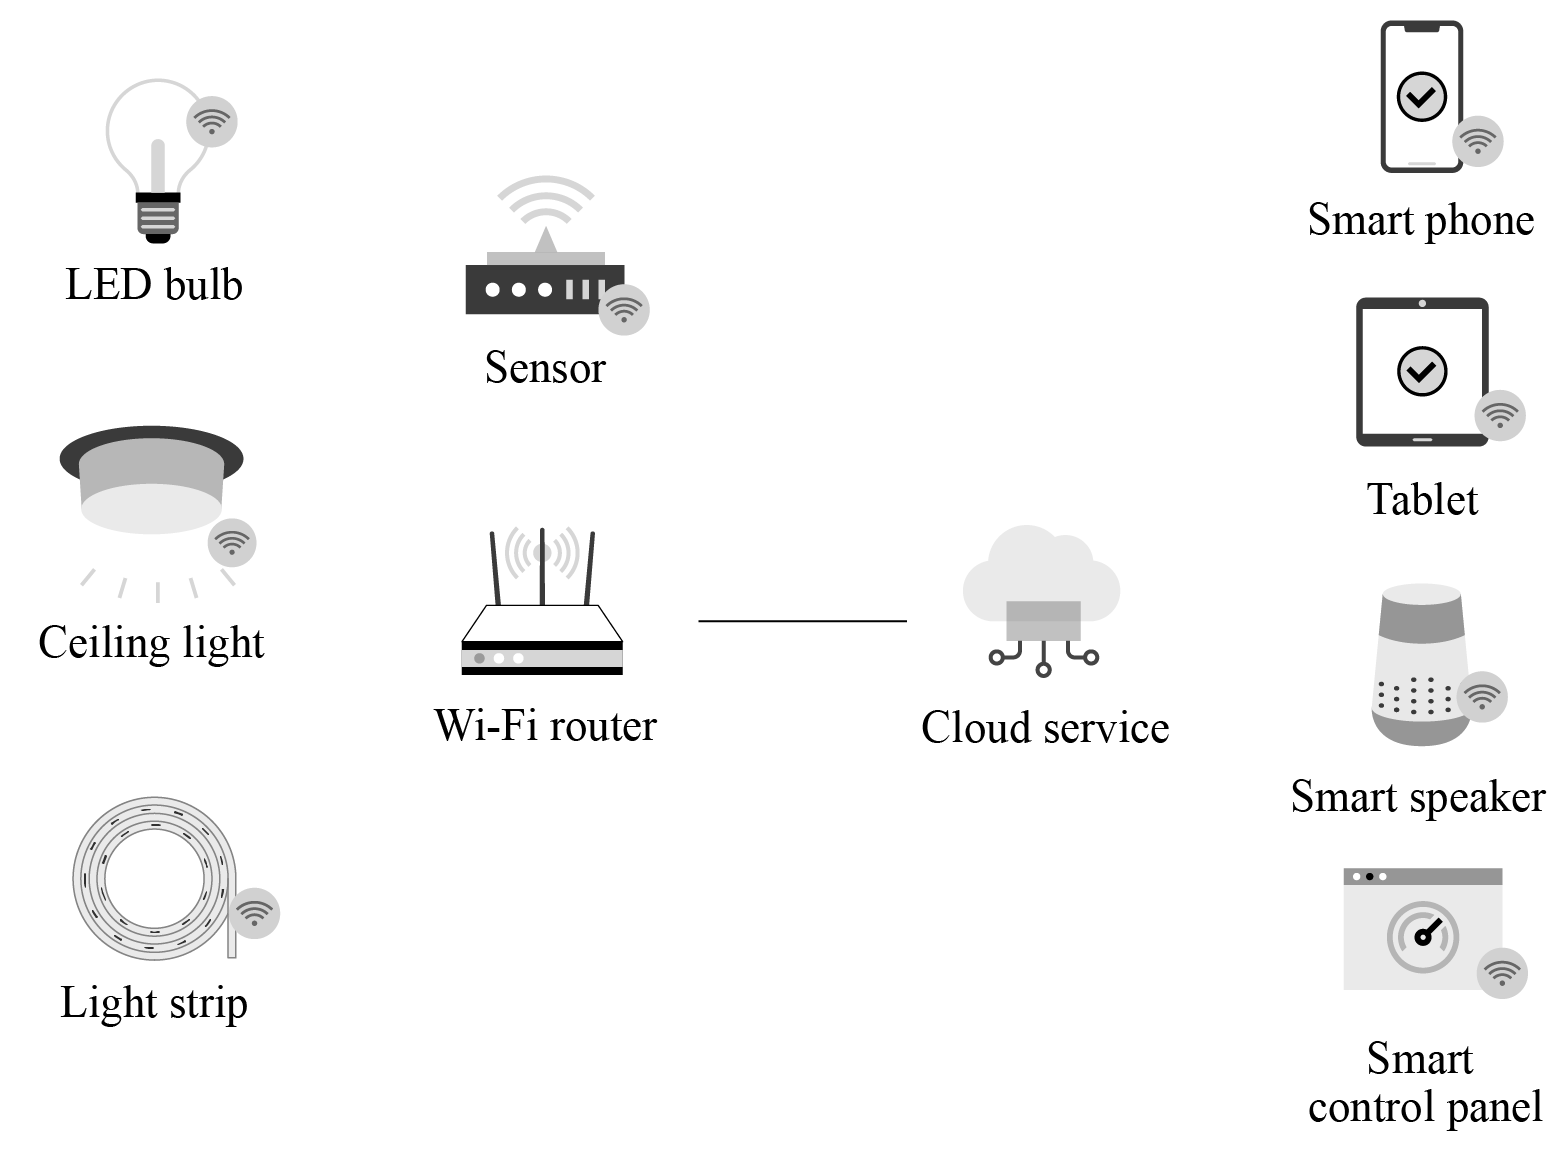
\includegraphics[width=0.6\textwidth]{D5Z/5-1}
    \caption{Structure of smart light system}
\end{figure}

From the description above, we can see that the main features of smart light products is to be controlled through wireless connection. Now we will take the colour-changing smart LED light as an example to explain the main components of smart light products and how to control them.

Figure 5.2 shows the structure of a smart LED bulb, including an E27 standard lamp holder, a plastic-wrapped aluminium lamp body, a power supply \& an LED driver board, a Wi-Fi module, LED beads \& an aluminium substrate, and a highly transparent lampshade. Compared with traditional LED bulbs, a smart LED bulb has an additional Wi-Fi module. So how does this Wi-Fi module help control the light wirelessly? The following sections will further elaborate on the functional implementation.

\begin{figure}[h!]
    \centering
    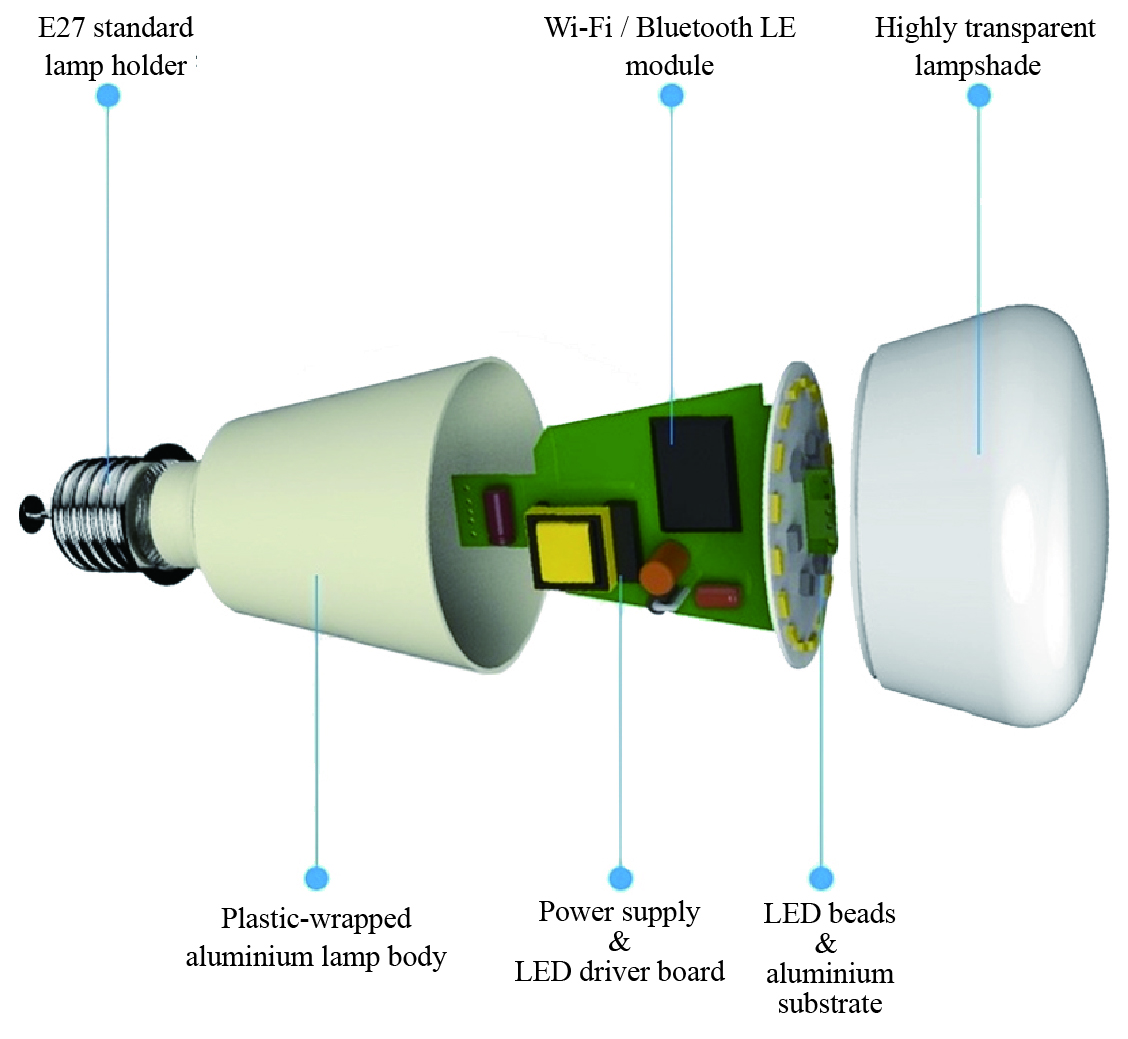
\includegraphics[width=0.55\textwidth]{D5Z/5-2}
    \caption{Structure of smart LED bulb}
\end{figure}

Figure 5.3 shows the functional block diagram of a smart LED bulb, which mainly includes a 220 V AC-DC power supply module, a constant-current LED driver, a 3.3 V output auxiliary power supply, a PWM control and wireless communication module, and LED beads of various colours.

\begin{figure}[h!]
    \centering
    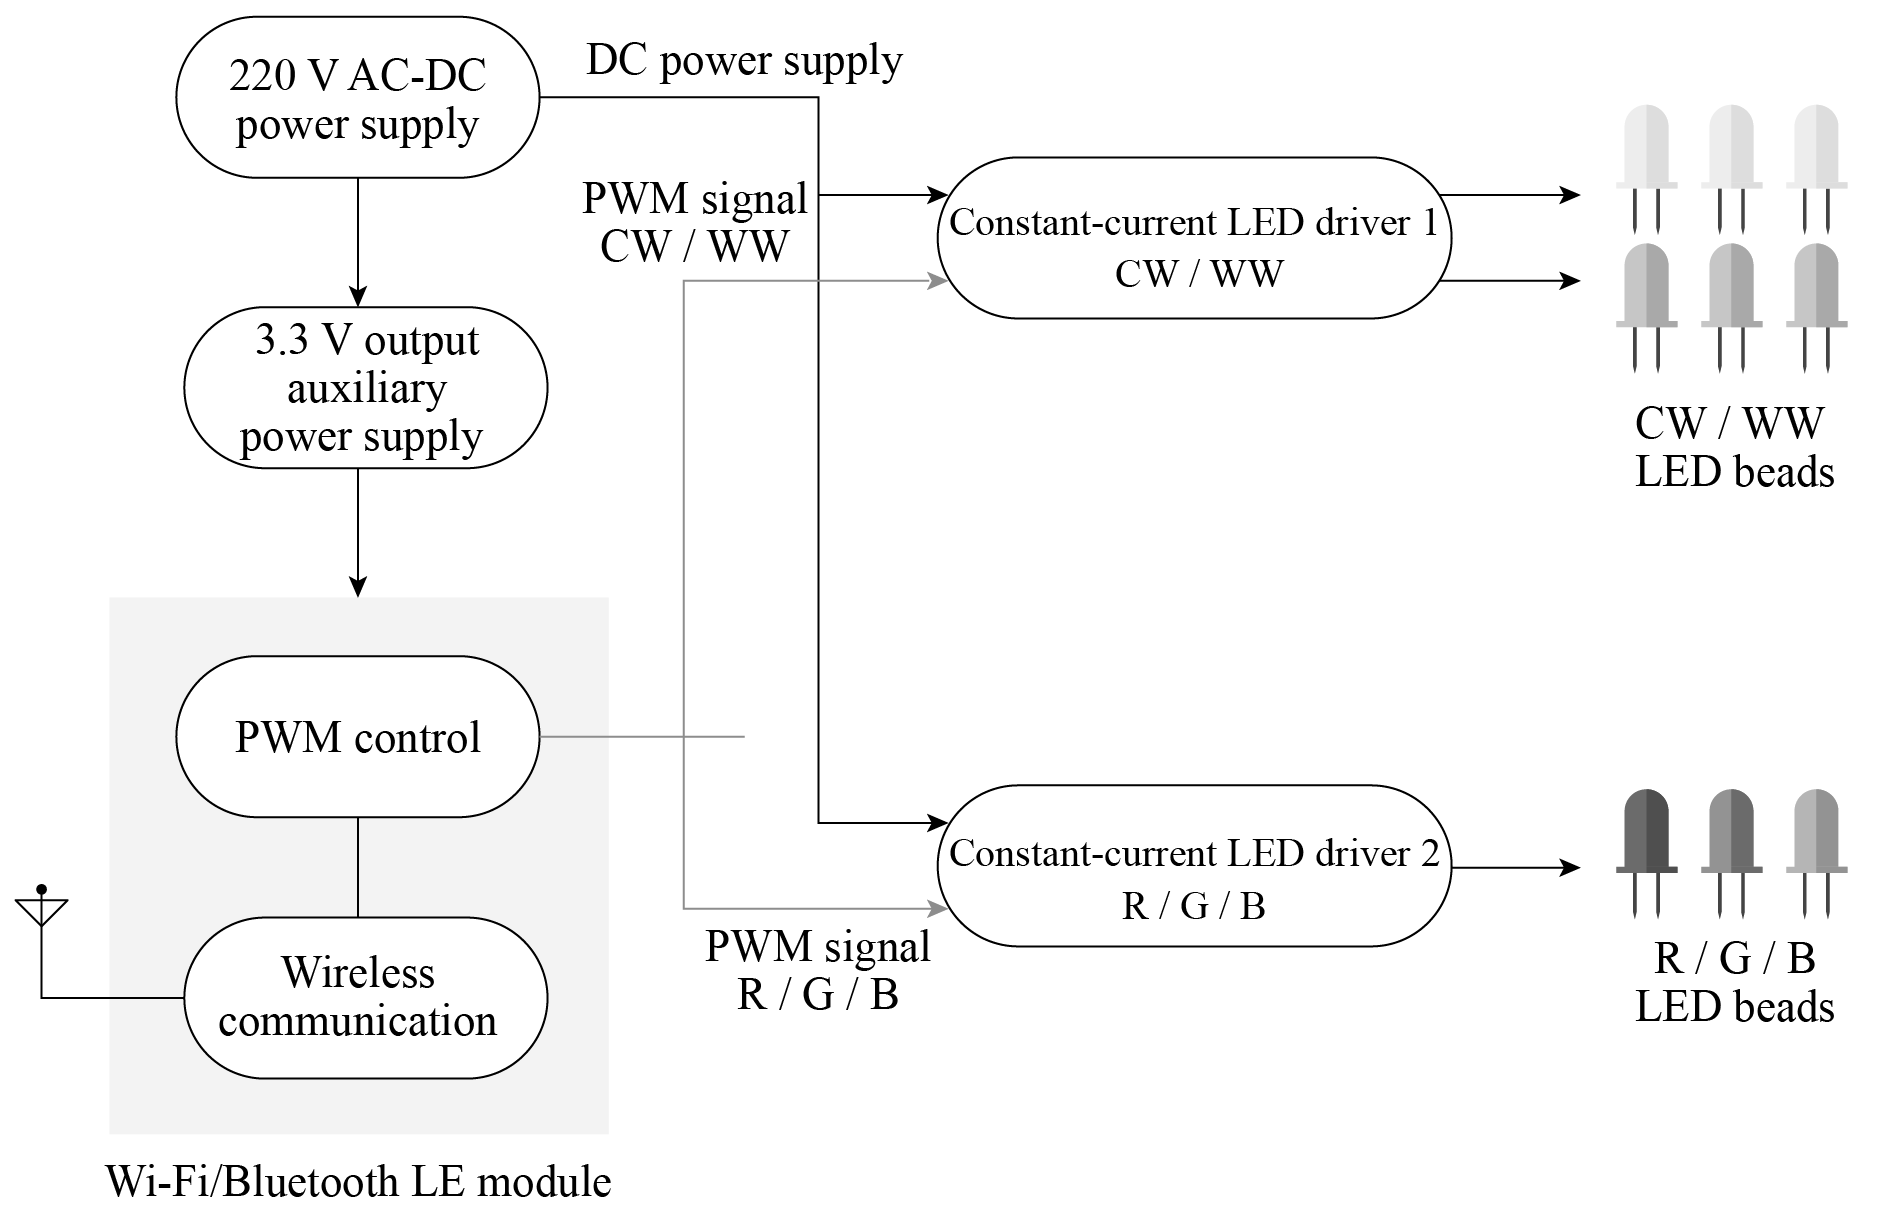
\includegraphics[width=0.7\textwidth]{D5Z/5-3}
    \caption{Block diagram of functional units for smart LED bulb}
\end{figure}

Before detailing each functional unit, let’s first take a glance at how they manage to change the brightness and colour of the lighting as a whole. The key lies in the LED lamp beads.

LED lamp beads can be dimmed in two ways: analogue dimming and digital dimming. Analogue dimming changes LED light output by simply adjusting the DC current in the circuit; while digital dimming, also known as PWM dimming, is achieved by varying the conduction time of forward current through turning on/off LEDs using PWM signals of different pulse widths. Section 6.3.3 will describe PWM dimming in detail. Here we will briefly introduce PWM dimming using PWM signals.

When using a controllable constant-current source to drive LED beads, to adjust colour temperature, you can change the duty cycles of PWM signals on two channels to adjust the current of warm-white (WW) and cool-white (CW) LED beads; to adjust light colours, you can change the duty cycles of PWM signals on three channels to adjust the brightness of corresponding colours so that the smart LED light emits the mixed colour of different lamp beads.

Knowing the basics of light dimming and colour change, now let’s dig into the functional units one by one.

\begin{term}{220 V AC-DC power supply}
    The input power of smart LED lights is usually high-voltage AC, and the standard household AC in China is 220 V. The 220 V AC-DC power module first converts the AC to DC through a rectifier bridge, and then reduces it to 18 $\sim$ 40 V for the constant-current LED drivers. Since the operating voltage of the PWM control and wireless communication module is 3.3 V, there is another auxiliary power supply to reduce the DC power to 3.3 V.
\end{term}

\begin{term}{Constant-current LED driver}
    To ensure consistency in the emission of multiple LED beads, you can use a series circuit and drive the LEDs with a constant current source. The brightness of the LEDs can be adjusted by controlling the constant current source using PWM signals. Constant-current LED driver 1 is used to drive the LEDs in cool white (CW) and warm white (WW), and the output power is relatively higher; constant-current LED driver 2 is used to drive red (R) / green (G) / blue (B) LEDs, mainly for changing colours, and the output power is lower.
\end{term}

\begin{term}{LED beads}
    In smart LED lights, there are usually warm-white, cool-white, red, green, and blue LED beads, among which more warm-white and cool-white beads are used for lighting, and less red, green or blue beads for colour adjustment.
\end{term}

\begin{term}{PWM control and wireless communication}
    In smart light products, to realise PWM control and wireless communication functions, a highly-integrated system-on-a-chip (SoC) is usually used. SoC supports multiple PWM signal outputs, as well as one or more mainstream wireless communication protocols such as Wi-Fi, Bluetooth LE, or ZigBee. It can run embedded RTOS, and supports software application development. With chips of Wi-Fi connectivity, you can connect your product to the Internet and cloud servers through a Wi-Fi router; with chips of Bluetooth LE or ZigBee functions, you need to configure a gateway device to connect to an Ethernet or Wi-Fi router first and then get it connected to the Internet and cloud servers.
\end{term}

The introduction above explains the main components of smart LED lights, as well as the realisation of dimming and colour change functions. It can be concluded that the biggest difference between smart light products and ordinary light products lies in the use of PWM control and wireless communication. The following sections of this chapter will focus on how to design the minimal hardware system based on the ESP32-C3 chip to realise PWM dimming, colour change, and wireless communication. The design is also applicable to other types of smart light products such as spotlights, ceiling lights, lamps, light strips, etc.

\section{Hardware Design of ESP32-C3 Core System}

Through Section 5.1, we can see that the PWM control and wireless communication module is the core unit of smart light products, which distinguishes them from traditional light products. Then how should we design this core system to implement the functions of smart light products? In this section, we’ll use the ESP32-C3 chip to demonstrate its hardware design.

ESP32-C3 is a highly-integrated SoC equipped with a 32-bit RISC-V processor, supporting 2.4 GHz Wi-Fi and Bluetooth LE connectivity. The functional block diagram of ESP32-C3 is shown in Figure 5.4.

\begin{figure}[h!]
    \centering
    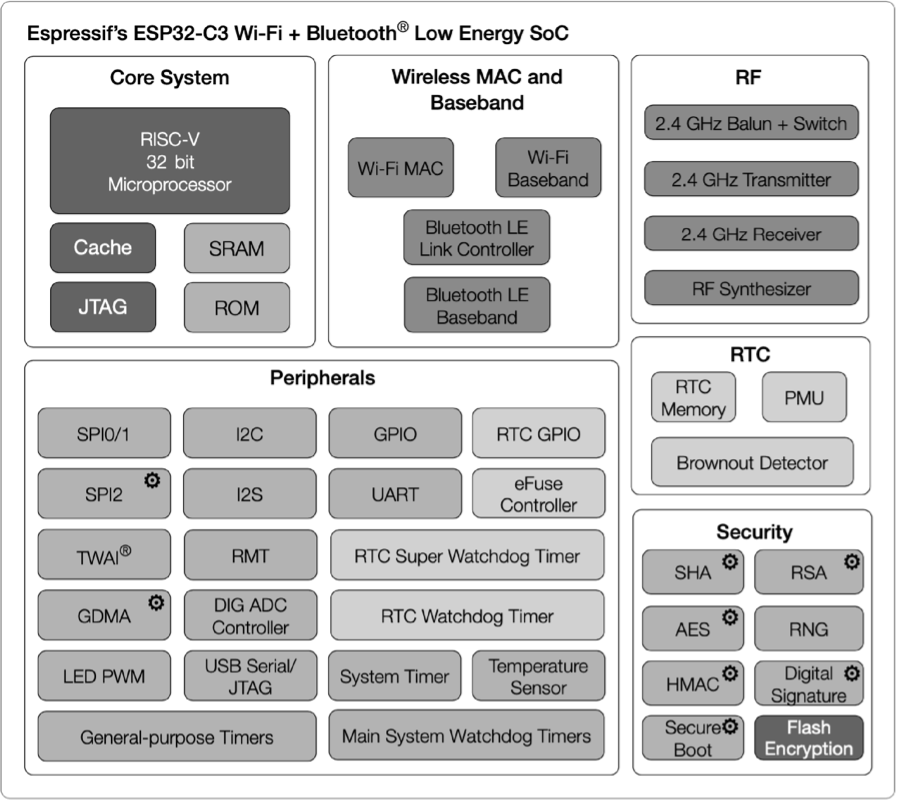
\includegraphics[width=0.65\textwidth]{D5Z/5-4}
    \caption{Block diagram of ESP32-C3 functions}
\end{figure}

ESP32-C3 has the following features:

\begin{itemize}
    \item A 32-bit RISC-V single-core processor with a four-stage pipeline which operates at up to 160 MHz.
    \item A \textbf{complete Wi-Fi subsystem} which complies with IEEE 802.11b/g/n protocol and supports Station mode, SoftAP mode, SoftAP + Station mode, and promiscuous mode.
    \item A \textbf{Bluetooth LE subsystem} which supports Bluetooth 5 and Bluetooth mesh.
    \item Storage capacities ensured by 400 KB SRAM and 384 KB ROM on the chip, and SPI, Dual SPI, Quad SPI, and QPI interfaces that allow connection to external flash.
    \item \textbf{Reliable security mechanisms} ensured by cryptographic hardware accelerators that support AES-128/256, Hash, RSA, HMAC, digital signature and secure boot, external memory encryption and decryption, random number generator, and permission control on accessing internal memory, external memory, and peripherals.
    \item \textbf{A rich set of peripheral interfaces} which are ideal for various scenarios and complex applications; \textbf{22 programmable GPIOs} that can be configured flexibly to support LED PWM, UART, I2C, SPI, I2S, ADC, TWAI, RMT, and USB Serial/JTAG applications.
\end{itemize}

The ESP32-C3 series of chips has several variants, including the version with in-package SPI flash. ESP8685 is a small package version of ESP32-C3, as shown in Table 5.1.


\begin{table}[h!]
    \renewcommand{\arraystretch}{1.2}
    \caption{ESP32-C3 series}
    \begin{tabular}{|>{\Centering}m{9em}|>{\Centering}m{9em}|>{\Centering}m{10em}|>{\Centering}m{10em}|}
        \hline
        \rowcolor{LightBlue} \textbf{MPN}&\textbf{Flash (MB)}&\textbf{Temp (℃)}&\textbf{Size (mm)}\\
        \hline
        ESP32-C3&—&--40 $\sim$ 105&QFN32 (5×5)\\
        \hline
        ESP32-C3-FN4&4&--40 $\sim$ 85&QFN32 (5×5)\\
        \hline
        ESP32-C3-FH4&4&--40 $\sim$ 105&QFN32 (5×5)\\
        \hline
        ESP32-C3-FH4AZ&4&--40 $\sim$ 105&QFN32 (5×5)\\
        \hline
        ESP8685H2&2&--40 $\sim$ 105&QFN32 (4×4)\\
        \hline
        ESP8685H4&4&--40 $\sim$ 105&QFN32 (4×4)\\
        \hline
    \end{tabular}
\end{table}

\note{\textbullet\ For ESP32-C3FH4AZ, ESP8685H2, and ESP8685H4, pins for flash connection are not bonded.

\textbullet\ Nomenclature of ESP32-C3 series: \textbf{F} stands for in-package flash, \textbf{H/N} indicates the flash temperature, and \textbf{AZ} is other identification code.}

The core circuit for ESP32-C3 requires about 20 resistors, capacitors, and inductors in total, as well as one crystal and one SPI flash. The high integration of ESP32-C3 makes it suitable for small-sized applications such as smart light products. Figure 5.5 and Figure 5.6 show the block diagram and the schematic of ESP32-C3 core circuit.

\begin{figure}[h!]
    \centering
    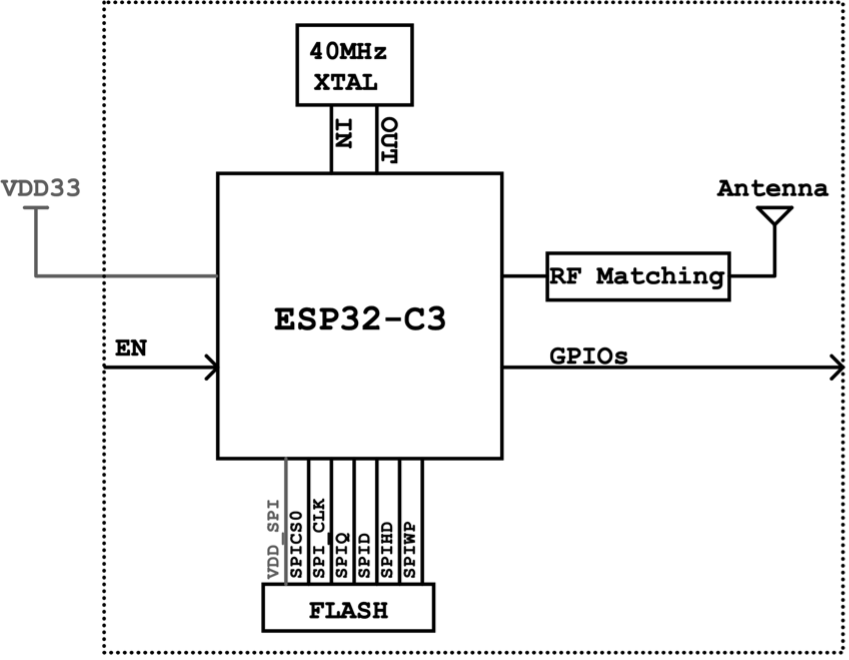
\includegraphics[width=0.55\textwidth]{D5Z/5-5}
    \caption{Block diagram of ESP32-C3 core circuit}
\end{figure}

The following explains in detail the schematics and PCB layout of ESP32-C3.

\begin{figure}[h!]
    \centering
    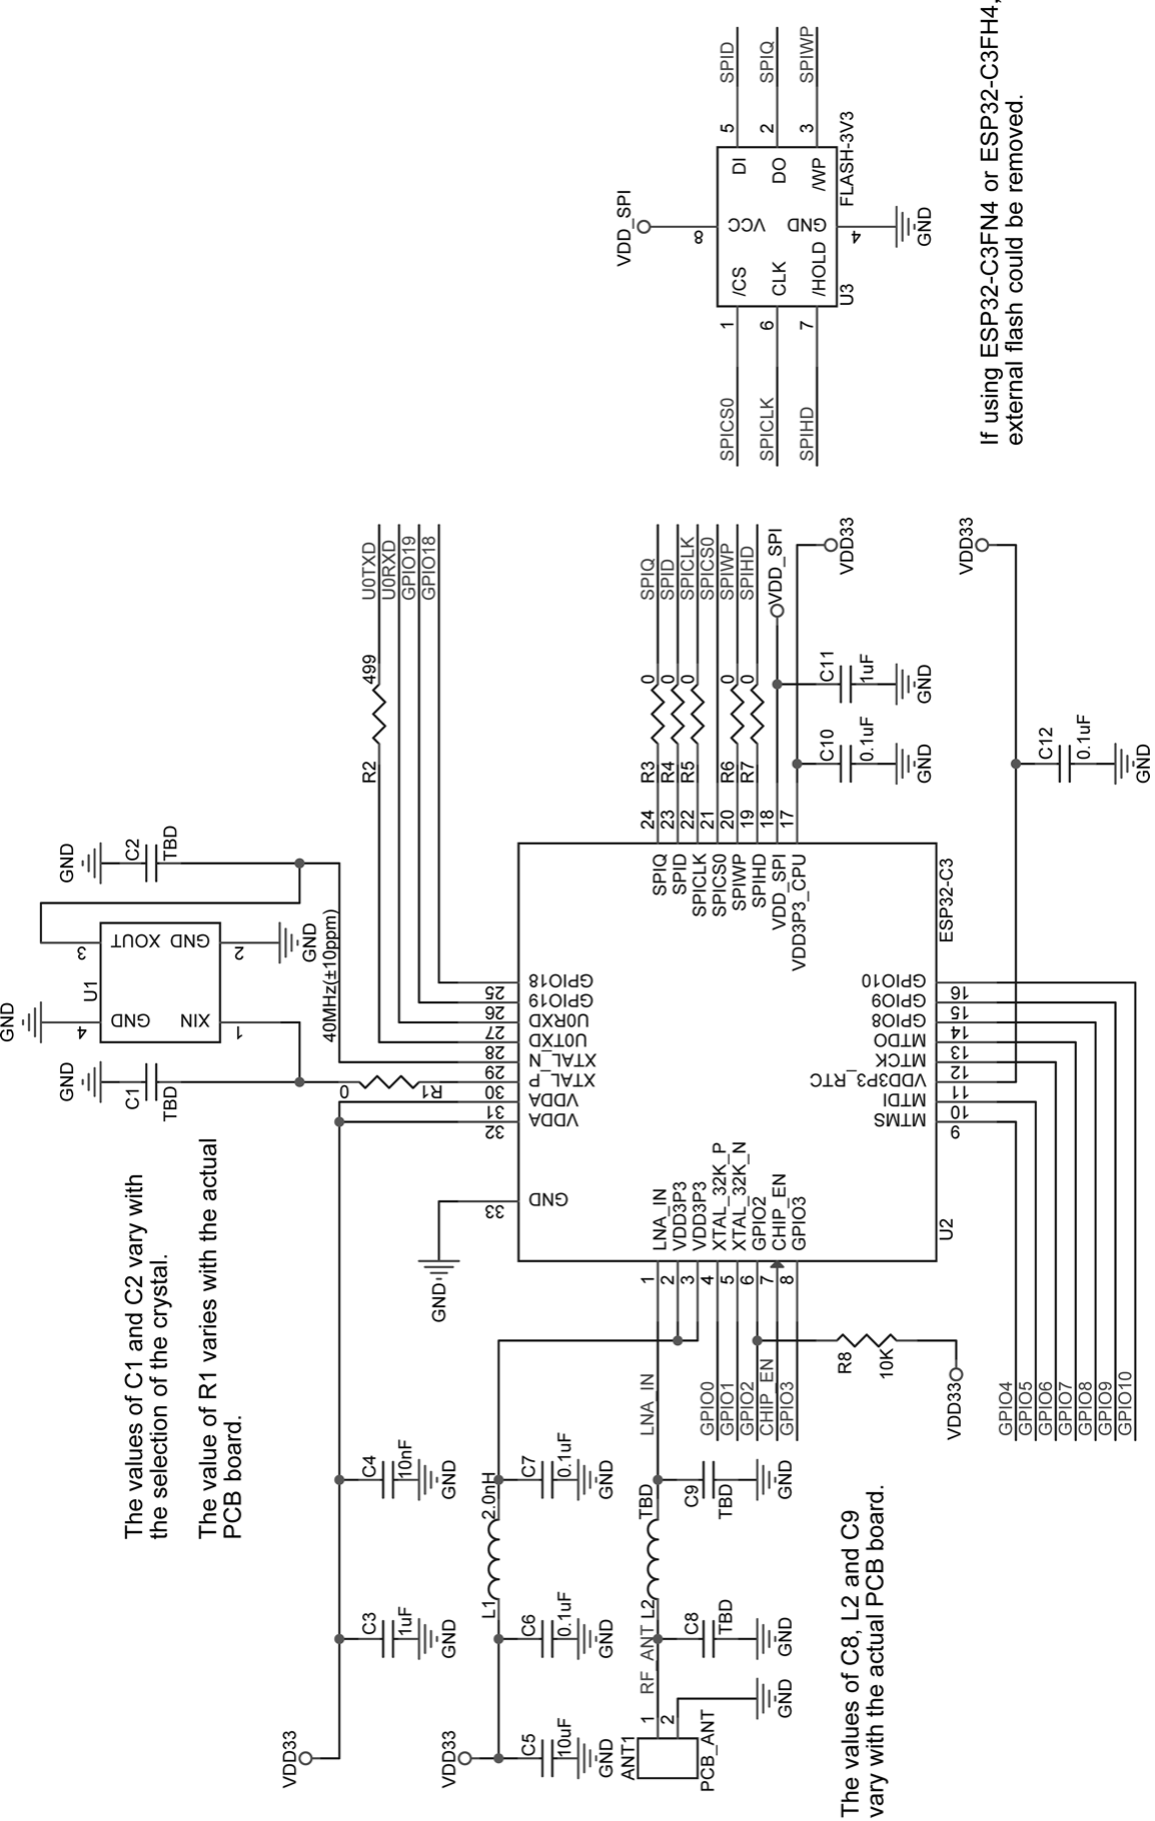
\includegraphics[width=0.83\textwidth]{D5Z/5-6}
    \caption{Schematic of ESP32-C3 core circuit}
\end{figure}

\subsection{Power Supply}
Pin 11 and pin 17 are the power supply pins for RTC IO and CPU IO respectively, in a voltage range of 3.0 V $\sim$ 3.6 V. We recommend adding a 0.1 $\mu$F capacitor close to each power supply pin. When working as an output power supply pin, VDD\_SPI (pin 18) mainly powers external SPI flash. We recommend adding a 1 $\mu$F filter capacitor between VDD\_SPI and ground. When VDD\_SPI works as the power supply pin for in-package flash or external 3.3 V flash, the voltage of VDD3P3\_CPU should be maintained at 3.0 V or above, to ensure the flash’s operation.

Pin 2, pin 3, pin 31, and pin 32 are the analogue power supply pins, working at 3.0 V $\sim$ 3.6 V. Please note that when ESP32-C3 works in transmission (TX) mode, the instantaneous current will be higher and may cause power rail collapse. Therefore, it is highly recommended to add a 10 $\mu$F capacitor to the power trace, which can work in conjunction with the 0.1 $\mu$F capacitor. In addition, an LC filter circuit needs to be added near pin 2 and pin 3 to suppress high-frequency harmonics. The inductor’s rated current is preferably 500 mA or above. Refer to the core circuit schematic and place the appropriate decoupling capacitor near each analogue power pin.

For a single power supply, the recommended voltage is 3.3 V, and the recommended output current is 500 mA or above. We also suggest adding an ESD protection diode at the power entrance.

\subsection{Power-on Sequence and System Reset}
ESP32-C3 uses a 3.3 V system power supply. The chip should be activated after the power rails have stabilised. This is achieved by delaying the activation of pin 7 CHIP\_EN after the 3.3 V rails have been brought up. Figure 5.7 shows the power-up and reset timing of ESP32-C3. Details about the parameters are listed in Table 5.2.

\begin{figure}[h!]
    \centering
    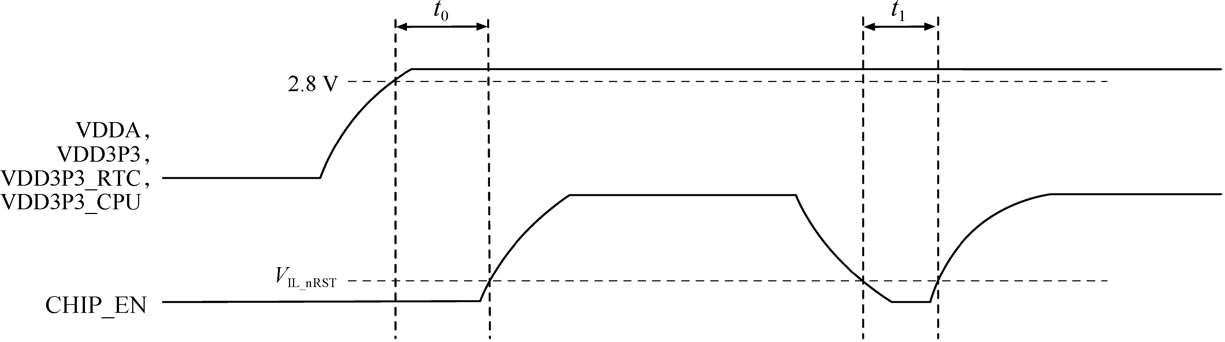
\includegraphics[width=\textwidth]{D5Z/5-7}
    \caption{ESP32-C3 power-up and reset timing}
\end{figure}

\begin{table}[h!]
    \renewcommand{\arraystretch}{1.4}
    \caption{Parameter description of ESP32-C3 power-up and reset timing}
    \begin{tabular}{|>{\Centering}m{5em}|m{29em}|>{\Centering}m{4em}|}
        \hline
        \rowcolor{LightBlue} \textbf{Parameter}&\multicolumn{1}{c|}{\textbf{Description}}&\textbf{Min.}\\
        \hline
        \textit{t$_0$}&Time between bringing up the VDDA, VDD3P3, VDD3P3\_RTC, and VDD3P3\_CPU rails, and activating CHIP\_EN&50 $\mu$s\\
        \hline
        \textit{t$_1$}&Duration of CHIP\_EN signal level $< V_{IL\_nRST}$ to reset the chip&50 $\mu$s\\
        \hline
    \end{tabular}
\end{table}

To ensure that the power supply to ESP32-C3 is stable during power-up, it is advised to add an RC delay circuit at the CHIP\_EN pin. The recommended setting for the RC delay circuit is usually $R = 10 k\Omega$ and $C = 1 \mu F$, while specific parameters should be adjusted based on the power-up timing of the power supply and the power-up and reset sequence timing of the chip.

CHIP\_EN can also be used as the reset pin of ESP32-C3. When CHIP\_EN is at low level, the reset voltage (V$_{IL\_nRST}$) should be (--0.3 $\sim$ 0.25) × $V_{DD}$ (where $V_{DD}$ is the I/O voltage for a particular power domain of pins). To avoid reboots caused by external interference, route the CHIP\_EN trace as short as possible, and add a pull-up resistor as well as a capacitor to ground. Note that CHIP\_EN pin must not be left floating.

\subsection{SPI Flash}
ESP32-C3 supports external flash of up to 16 MB, which is mainly used for storing program firmware, system parameters, user parameters, user data, etc. The SPI flash is powered by VDD\_SPI. We recommend reserving a serial resistor (initially of 0 $\Omega$) on the SPI line, to lower the driving current, adjust timing, reduce crosstalk and external interference, etc. ESP32-C3FH4/FN4 has an in-package 4 MB SPI flash.

\subsection{Clock Source}
Currently, the ESP32-C3 firmware supports 40 MHz crystal. The specific capacitance of C1 and C2 depends on further testing of, and adjustment to, the overall performance of the whole circuit. Please add a component (i.e., R1 in Figure 5.6) in series on the XTAL\_P clock trace to minimise the impact of crystal harmonics on RF performance. The value of this component (initially of 24 nH) depends on further RF testing. Note that the accuracy of the selected crystal needs to be ±10 ppm. In actual use, as the temperature of smart light products rises, the frequency deviation of the crystal will also increase. Therefore, please ensure that the frequency deviation of the crystal does not exceed 25 ppm, so as not to affect Wi-Fi communication.

Although ESP32-C3 has integrated an RC oscillator as the RTC clock source, it also supports an external 32.768 kHz crystal to act as the RTC clock source. Figure 5.8 shows the schematic of the external 32.768 kHz crystal.

\begin{figure}[h!]
    \centering
    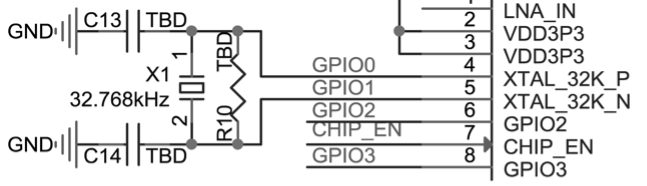
\includegraphics[width=0.7\textwidth]{D5Z/5-8}
    \caption{Schematic of ESP32-C3’s external crystal (RTC)}
\end{figure}

\note{
\textbullet\ Requirements for the 32.768 kHz crystal: 

\leftskip 2em
- Equivalent series resistance (ESR) $\leq$ 70 k$\Omega$.

- Load capacitance at both ends should be configured according to the crystal’s specification.

\leftskip 1em
\textbullet\ The parallel resistor R10 is used for biasing the crystal circuit ($5 M\Omega < R10 \leq 10 M\Omega$). In general, you do not need to populate R10.

\textbullet\ If the RTC source is not required, then pin 4 (XTAL\_32K\_P) and pin 5 (XTAL\_32K\_N) can be used as normal GPIOs.}

\subsection{RF and Antenna}
In your circuit design, please add a $\pi$-matching network between the RF port (LNA\_IN) and the antenna, for antenna matching purpose. A CLC network is preferred, as shown in Figure 5.9. The parameters of C8, L2, and C9 in the matching network are subject to the actual antenna and PCB layout.

\begin{figure}[h!]
    \centering
    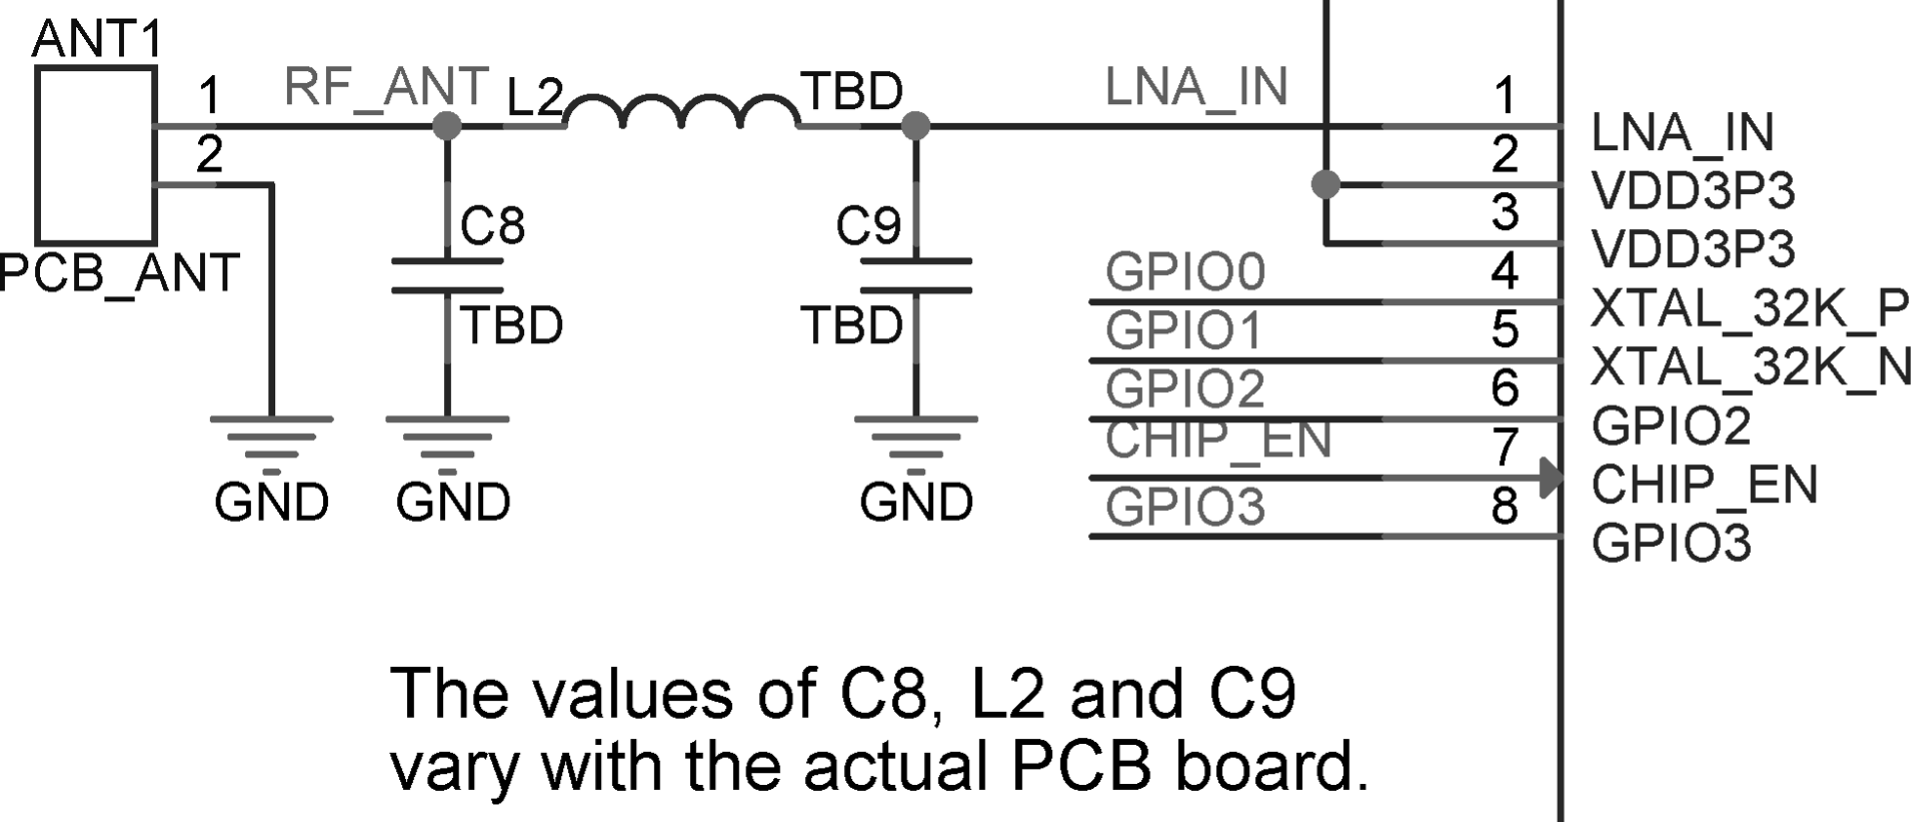
\includegraphics[width=0.7\textwidth]{D5Z/5-9}
    \caption{CLC circuit for ESP32-C3 RF matching}
\end{figure}

The antenna can be selected based on product design and the overall cost. You can choose PCB onboard antenna, or an external antenna such as rod antenna, FPC antenna, ceramic antenna, 3D metal antenna, etc. Commonly-used antenna types are shown in Figure 5.10. Their installation methods and characteristics are provided in Table 5.3.

\begin{figure}[h!]
    \centering
    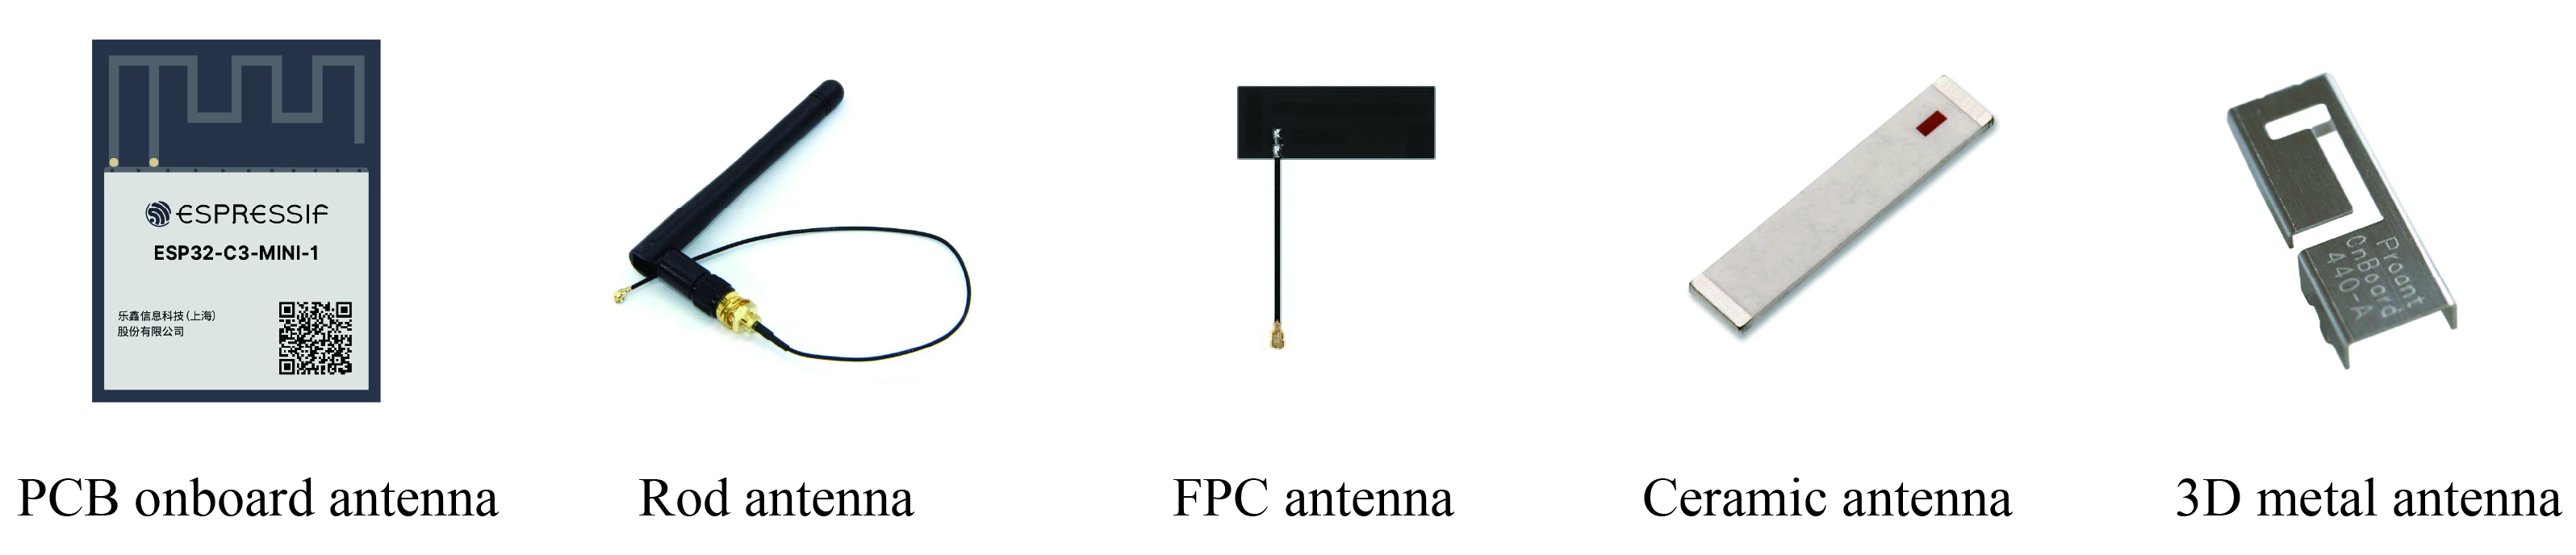
\includegraphics[width=0.9\textwidth]{D5Z/5-10}
    \caption{Commonly-used antenna types}
\end{figure}

\begin{table}[h!]
    \renewcommand{\arraystretch}{1.2}
    \caption{Installation methods and characteristics of commonly-used antenna types}
    \begin{tabular}{|>{\Centering}m{8em}|>{\Centering}m{10em}|>{\RaggedRight}m{20.5em}|}
        \hline
        \rowcolor{LightBlue} \textbf{Antenna Type}&\textbf{Installation Methods}&\multicolumn{1}{c|}{\textbf{Characteristics}}\\
        \hline
        PCB\newline onboard antenna&PCB onboard&Low cost, medium gain, usually integrated on modules\\
        \hline
        Rod antenna&External connection\newline through I-PEX connector&High cost, high gain, less susceptible to interference, good omni-directional performance\\
        \hline
        FPC antenna&Adhesive installation&Medium cost, medium gain, can be adhered to the package, suitable for products with restricted structure\\
        \hline
        Ceramic antenna&PCB mounting&Medium cost, low gain, small size, suitable for small-sized modules\\
        \hline
        3D metal antenna&PCB mounting&High cost, high gain, less susceptible to interference, good omni-directional performance\\
        \hline
    \end{tabular}
\end{table}

The RF performance can be optimised through antenna matching. After matching, you can use CMW500, WT-200, IQ View, IQ Xel or other comprehensive RF testers to test RF performance of the ESP32-C3 core board. RF test includes conducted test and radiatied test.

\begin{term}{Conducted test}
    In conducted tests, use a 50 $\Omega$ RF cable to connect the RF output port of the ESP32-C3 core board to the tester’s RF port, and run the RF test software on the PC. Through the software, you can communicate with the ESP32-C3 core board and the tester, thus controlling the test. The conducted test set-up is shown in Figure 5.11.

    \begin{figure}[h!]
        \centering
        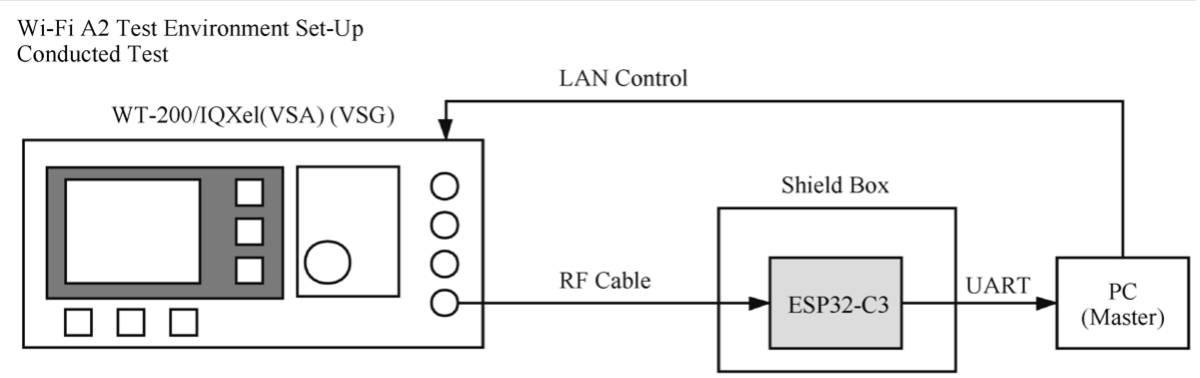
\includegraphics[width=\textwidth]{D5Z/5-11}
        \caption{Conducted test set-up for ESP32-C3 core board}
    \end{figure}
\end{term}

\begin{term}{Radiated test}
    When performing a radiated test, place the tester’s antenna and ESP32-C3 board’s antenna close to each other in the shield box. It is recommended that the distance between the two antennas be about 10 cm. Control the test through PC software. The radiated test set-up is shown in Figure 5.12.

    \begin{figure}[h!]
        \centering
        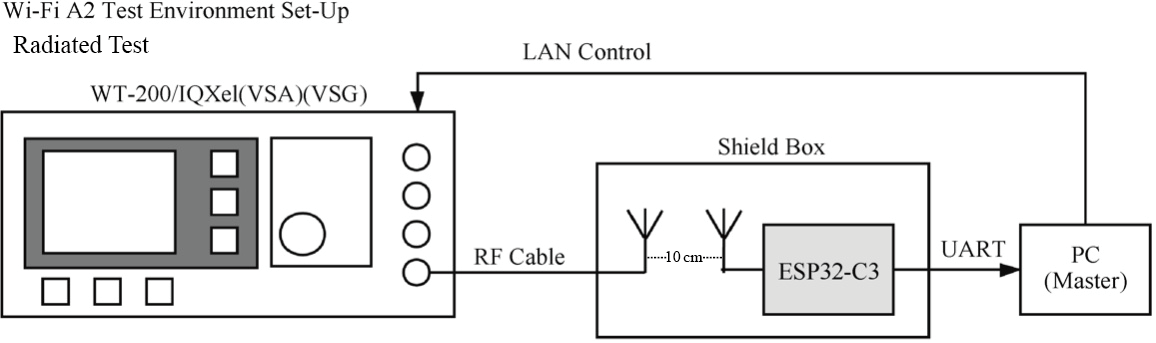
\includegraphics[width=\textwidth]{D5Z/5-12}
        \caption{Radiated test set-up for ESP32-C3 core board}
    \end{figure}
\end{term}

For Wi-Fi RF performance test, the primary test parameters are target transmit power, EVM, receiver sensitivity, and frequency error, as shown in Table 5.4.

\begin{table}[h!]
    \renewcommand{\arraystretch}{1.5}
    \caption{Key parameters for Wi-Fi RF test}
    \begin{tabular}{|>{\Centering}m{12.5em}|>{\Centering}m{6.5em}|>{\Centering}m{5em}|>{\Centering}m{7em}|>{\Centering}m{6.5em}|}
        \hline
        \rowcolor{LightBlue} \textbf{Working Mode and Rate}&\textbf{Target TX Power (dBm)}&\textbf{EVM (dB)}&\textbf{Receiver Sensitivity (dBm)}&\textbf{Frequency Error (ppm)}\\
        \hline
        IEEE 802.11b, 1 Mbit/s&21.0±2.0&$<-$24.5&$<-$98&±25\\
        \hline
        IEEE 802.11g, 54 Mbit/s&19.0±2.0&$<-$27.5&$<-$76.2&±20\\
        \hline
        IEEE 802.11n, MCS7 HT20&18.5±2.0&$<-$29&$<-$74.4&±20\\
        \hline
        IEEE 802.11n, MCS7 HT40&18.5±2.0&$<-$28&$<-$71.2&±20\\
        \hline
    \end{tabular}
\end{table}

Figure 5.13 shows the spectral mask requirements in different working modes.

\begin{figure}[h!]
    \centering
    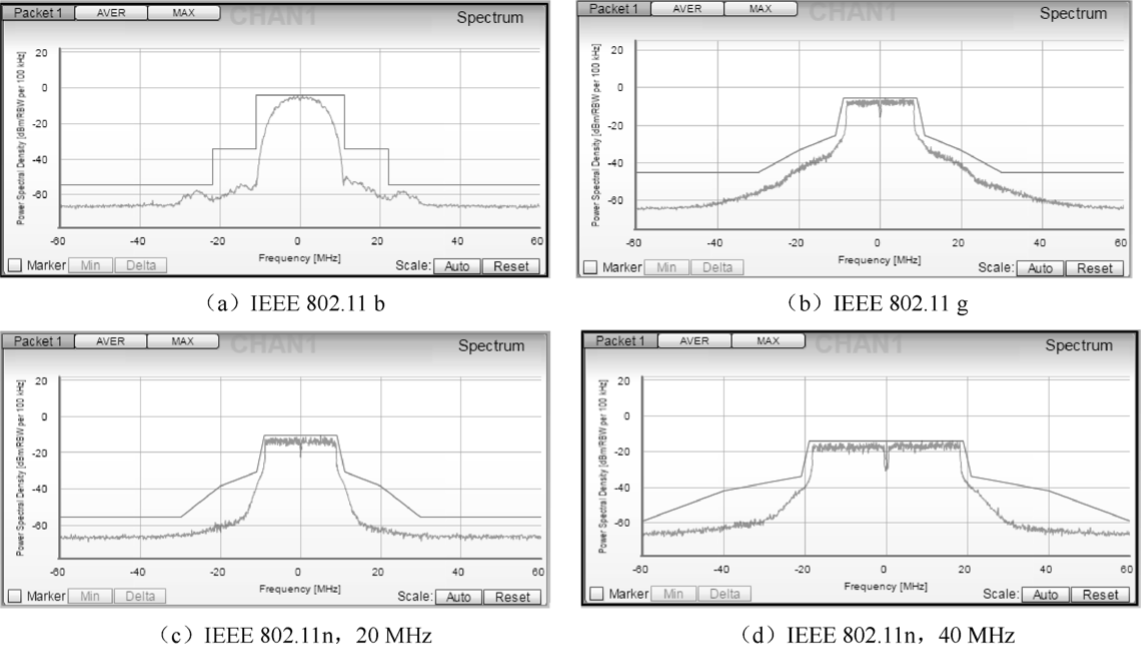
\includegraphics[width=0.9\textwidth]{D5Z/5-13}
    \caption{Spectral mask requirements in different working modes}
\end{figure}

\subsection{Strapping Pins}
ESP32-C3 has three strapping pins: GPIO2, GPIO8, and GPIO9. During the chip’s system reset, the strapping pins sample their voltage levels and store them into the latch until the chip is powered down or shut down. Depending on the stored voltage levels, the chip will enter different boot modes after system reset. The correspondence between the voltage levels and the boot modes is shown in Table 5.5. After reset, the strapping pins function as normal pins.

\begin{table}[h!]
    \renewcommand{\arraystretch}{1.2}
    \caption{Voltage level of strapping pins and corresponding boot mode}
    \begin{tabular}{|>{\Centering}m{8em}|>{\Centering}m{10em}|>{\Centering}m{10em}|>{\Centering}m{10em}|}
        \hline
        \rowcolor{LightBlue} \textbf{Strapping Pins}&\textbf{Default}&\textbf{SPI Boot}&\textbf{Download Boot}\\
        \hline
        GPIO2&N/A&1&1\\
        \hline
        GPIO8&N/A&Irrelevant&1\\
        \hline
        GPIO9&Weak internal pull-up&1&0\\
        \hline
    \end{tabular}
\end{table}

\subsection{GPIO and PWM Controller}
ESP32-C3 has 22 GPIO pins which can be assigned various functions by configuring corresponding registers. All GPIOs can be configured with internal pull-up, pull-down, or set to high impedance. GPIO MUX and GPIO Matrix are used to collectively control the GPIO pin signals of the chip. By utilising GPIO MUX and GPIO Matrix (as shown in Figure 5.14), it is possible to configure the peripheral input signals from any GPIO pin, and the peripheral output signals can also be connected to any GPIO pin.

\begin{figure}[h!]
    \centering
    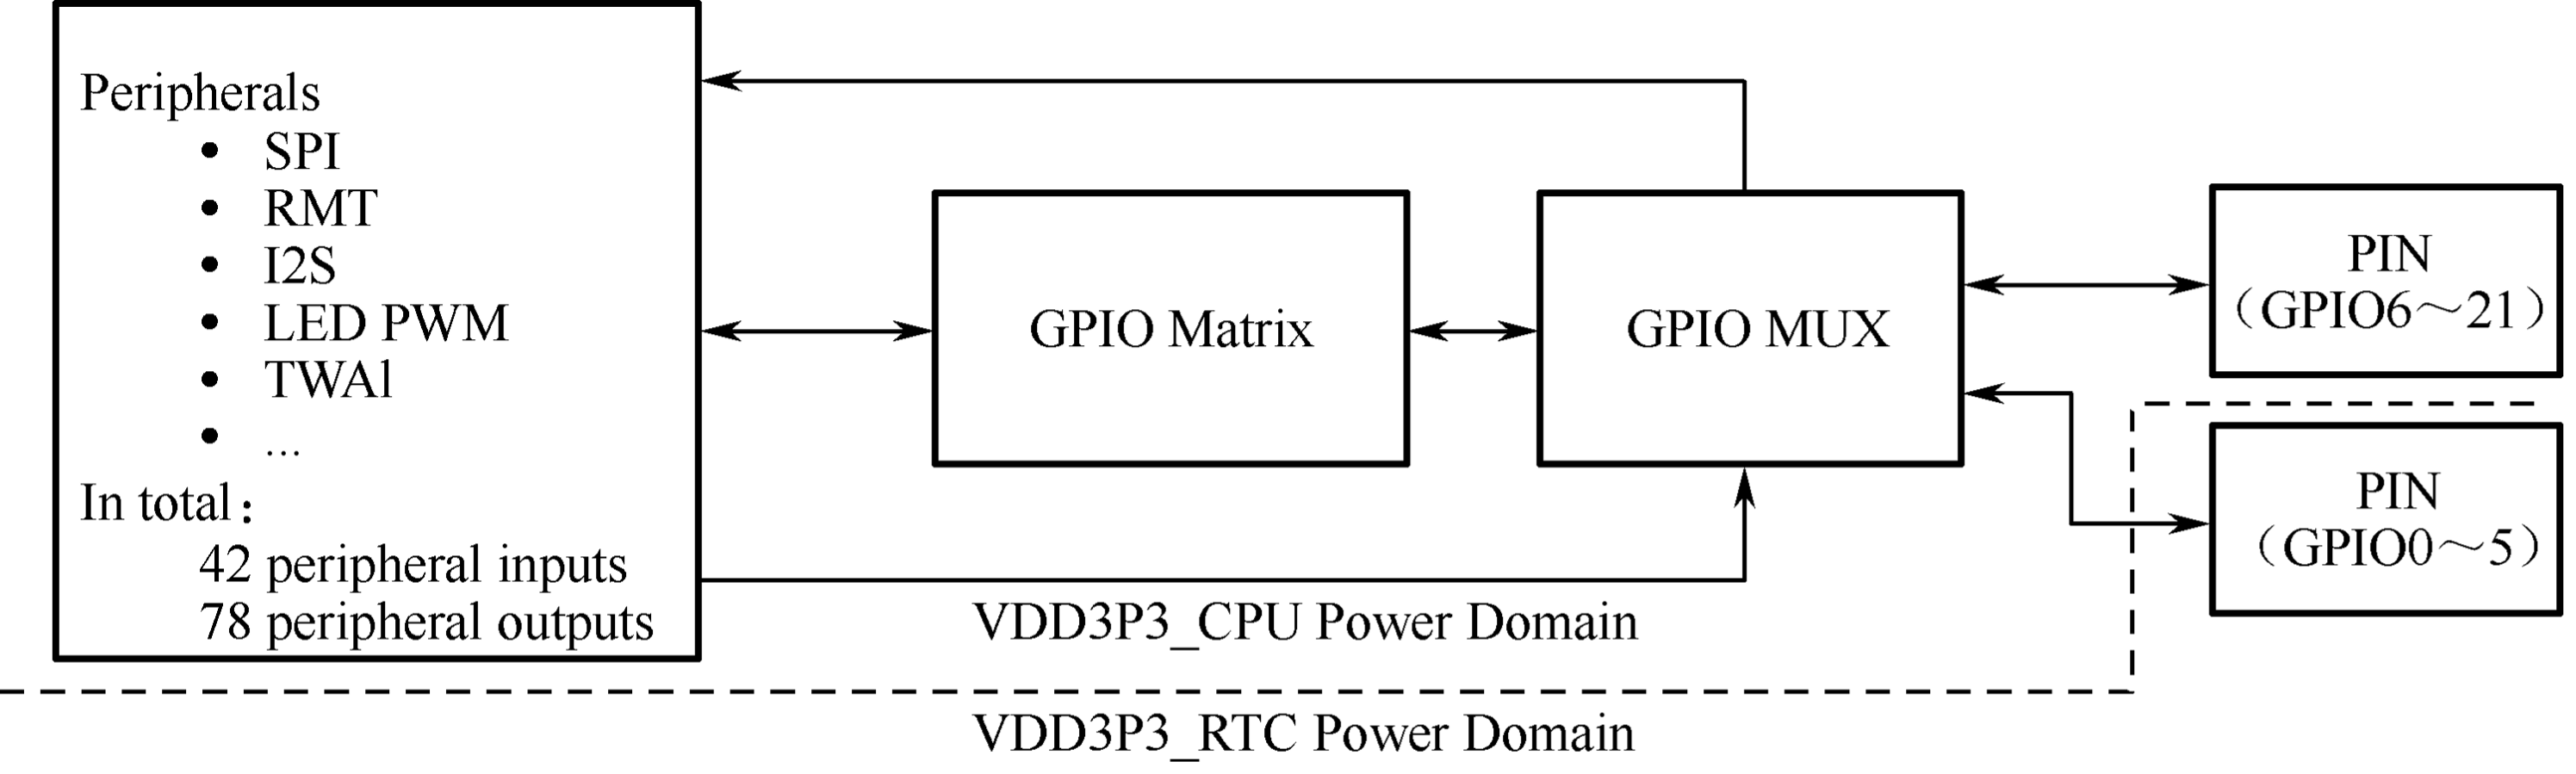
\includegraphics[width=0.9\textwidth]{D5Z/5-14}
    \caption{IO MUX and GPIO matrix}
\end{figure}

The PWM controller can generate independent PWM signals on six channels, which can be configured to any GPIO pins through the GPIO Matrix.

\section{Practice: Building a Smart Light System with ESP32-C3}
Section 5.2 introduced how to design the minimum hardware system (core circuit) and communication system for smart light products based on ESP32-C3. This minimum hardware system includes the main peripheral components and the antenna part which needs to be matched with the network analyser and RF tester according to the selected antenna type and the design of RF circuit. Antenna matching may be difficult for users who are new to RF. So, is there a ready-made minimum hardware system which has been tuned for RF performance, for users to get started quickly to develop a smart light product?

Yes, there ARE hardware modules based on the ESP32-C3 chip ready for operation. Apart from the chip, these modules also integrate a crystal oscillator, flash, antenna, RF circuit and main peripheral components. In addition, the modules have passed certification of SRRC, CE, FCC, and KCC, and can be directly applied to smart light products. In the following sections, we will choose one of the ESP32-C3 modules for smart light products design.

\subsection{Selecting Modules}
As shown in Table 5.6, in terms of the type of antenna, ESP32-C3 modules can be divided into PCB antenna modules and IPEX external antenna modules; in terms of size and pins, they can be divided into WROOM series and MINI series. Each module has two temperature range versions: --40 $\sim$ 85 ℃ version and --40 $\sim$ 105 ℃ version, suitable for smart lights of different temperature requirements. For lighting products such as LED bulbs which characterise high internal temperature, it is recommended to use the --40 $\sim$ 105 ℃ module. For other lighting products which do not have high internal temperature, the --40 $\sim$ 85 ℃ module is suitable.

\begin{table}[h!]
    \renewcommand{\arraystretch}{1.4}
    \caption{ESP32-C3 modules}
    \begin{tabular}{|>{\Centering}m{11em}|>{\Centering}m{11em}|>{\Centering}m{8em}|>{\Centering}m{8em}|}
        \hline
        \rowcolor{LightBlue} \textbf{Module}&\textbf{Antenna}&\textbf{Temp (℃)}&\textbf{Size (mm)}\\
        \hline
        \textbf{ESP32-C3-WROOM-02}\newline\vspace{6pt}\includegraphics[width=0.21\textwidth]{D5Z/02}&PCB antenna&--40 $\sim$ 85 ℃/\newline--40 $\sim$ 105 ℃&18×20×3.2\\
        \hline
        \textbf{ESP32-C3-WROOM-02U}\newline\vspace{6pt}\includegraphics[width=0.21\textwidth]{D5Z/02U}&IPEX external antenna&--40 $\sim$ 85 ℃/\newline--40 $\sim$ 105 ℃&18×14.3×3.2\\
        \hline
        \textbf{ESP32-C3-MINI-1}\newline\vspace{6pt}\includegraphics[width=0.21\textwidth]{D5Z/1}&PCB antenna&--40 $\sim$ 85 ℃/\newline--40 $\sim$ 105 ℃&13.2×16.6×2.4\\
        \hline
       \textbf{ ESP32-C3-MINI-1U}\newline\vspace{6pt}\includegraphics[width=0.21\textwidth]{D5Z/1U}&IPEX external antenna&--40 $\sim$ 85 ℃/\newline--40 $\sim$ 105 ℃&13.2×12.5×2.4\\
        \hline
    \end{tabular}
\end{table}

\note{You can also select one module from ESP8685-WROOM-01 to ESP8685-WROOM-07 series for a smaller package. For more information, please visit \href{https://products.espressif.com/\#/}{products.espressif.com}.}

\subsection{Configuring GPIOs of PWM Signals}
The PWM controller of ESP32-C3 can generate independent PWM signals on six channels, which can be assigned to any GPIOs through the GPIO matrix. In our design, five channels of PWM signals are used to control R (red), G (green), B (blue), CW (cool white), and WW (warm white) signals. In real application, we can use one channel to control the duty cycles of WW and CW LEDs to adjust the colour temperature, and another channel to control the total current to adjust the brightness of WW and CW LEDs. The GPIO configuration of each PWM signal is shown in Table 5.7.

\begin{table}[h!]
    \renewcommand{\arraystretch}{1.4}
    \caption{GPIO configuration for PWM signals}
    \begin{tabular}{|>{\Centering}m{0.48\textwidth}|>{\Centering}m{0.5\textwidth}|}
        \hline
        \rowcolor{LightBlue} \textbf{Function}&\textbf{GPIO Configuration}\\
        \hline
        R (Red)&GPIO3\\
        \hline
        G (Green)&GPIO4\\
        \hline
        B (Blue)&GPIO5\\
        \hline
        CW (Cool white)&GPIO7\\
        \hline
        WW (Warm white)&GPIO10\\
        \hline
    \end{tabular}
\end{table}

When selecting GPIOs, make sure that they are not at high level after chip start-up, otherwise the LED bulb may flicker when powered on. If no suitable GPIO is available, add a 10 k$\Omega$ pull-down resistor to the GPIO to prevent flickering. Any GPIOs on ESP32-C3 can be used for PWM function, as long as they are configured during initialisation after chip power-up.

Figure 5.15 shows the minimum control system based on the ESP32-C3-WROOM-02 module, which is connected to five LEDs of red, green, blue, cool white, and warm white.

\begin{figure}[h!]
    \centering
    \includegraphics[width=0.9\textwidth]{D5Z/5-15}
    \caption{Minimum control system based on ESP32-C3-WROOM-02}
\end{figure}

\subsection{Downloading Firmware and Debugging Interface}
\subsubsection{1. Connect ESP32-C3 to a PC.}
The ESP32-C3 chip integrates a USB Serial/JTAG controller which makes external USB-to-UART bridge or JTAG adapter unnecessary. The USB on ESP32-C3 uses GPIO19 as D+ and GPIO18 as D--, and can be directly connected to the USB interface on the PC, so as to realise firmware download, log printing, and JTAG debugging. Figure 5.16 shows that an ESP32-C3 board is connected to a PC through the built-in USB Serial/JTAG controller. You may visit \url{https://bookc3.espressif.com/usb} for more applications of the USB Serial/JTAG controller.

\begin{figure}[h!]
    \centering
    \includegraphics[width=0.65\textwidth]{D5Z/5-16}
    \caption{ESP32-C3 and PC connected through USB Serial/JTAG controller}
\end{figure}

For some ESP32-C3 development boards, a USB-to-UART bridge has been connected to the UART0 interface of the chip. Developers only need to connect the USB interface of the PC to the development board through the bridge, to realise firmware download and log printing, as shown in Figure 5.17.

\begin{figure}[h!]
    \centering
    \includegraphics[width=0.65\textwidth]{D5Z/5-17}
    \caption{USB-to-UART bridge connecting ESP32-C3 development board and PC}
\end{figure}

As for a finished board, to save its space and cost, we often use a programmer with USB-to-UART bridge to connect to the UART0 interface on the ESP32-C3 chip, to implement firmware download and log printing. Figure 5.18 shows that a programmer with USB-to-UART bridge is used to connect the development board and the PC.

\begin{figure}[h!]
    \centering
    \includegraphics[width=0.65\textwidth]{D5Z/5-18}
    \caption{Programmer with USB-to-UART bridge connecting ESP32-C3 and PC}
\end{figure}

\subsubsection{2. Download firmware.}
The firmware and system parameters of ESP32-C3 are stored in the SPI flash. To flash firmware into the chip, first put the chip in download boot mode. According to Table 5.5, GPIO2 and GPIO8 should be at high level, and GPIO9 should be at low level. Reset the chip to enter download boot mode. Connect ESP32-C3 to the PC using any of the three methods above to start firmware download.

\subsubsection{3. Debug interface.}

There are two ways to debug interface: log printing over serial port and JTAG debugging. 

\begin{term}{Log printing over serial port}
    ESP32-C3 ROM code and IDF SDK output log messages through UART0 by default. Connect ESP32-C3 and the PC with any of the three methods above to enable logging in the PC’s terminal.
\end{term}

\begin{term}{JTAG debugging}
    You can directly use the USB JTAG controller integrated in ESP32-C3 for debugging. To do this, you need to connect the JTAG pins – MTMS/GPIO4, MTDI/GPIO5, MTCK/GPIO6, and MTDO/GPIO7 – to an external JTAG adapter to implement debugging.
\end{term}

\subsection{Guidelines for RF Design}
When designing a smart light product using a module with PCB onboard antenna, pay attention to its placement on the base board to minimize the impact of the board on its antenna performance. The module should be placed as close to the edge of the base board as possible. It’s best to place the PCB antenna area outside the base board and keep its feed point closest to the board.

The antenna feed point of ESP32-C3-WROOM-02 is on the right, while that of ESP32-C3-MINI-1 is on the left. The placement of these two modules is shown in Figure 5.19 and 5.20.

\begin{figure}[h!]
    \centering
    \includegraphics[width=0.6\textwidth]{D5Z/5-19}
    \caption{ESP32-C3 module on base board - antenna feed point on the right}
\end{figure}

\begin{figure}[h!]
    \centering
    \includegraphics[width=0.6\textwidth]{D5Z/5-20}
    \caption{ESP32-C3 module on base board - antenna feed point on the left}
\end{figure}

\note{For feed points on the right (as in Figure 5.19), position \circled{3} and \circled{4} are preferred. For feed points on the left (as in Figure 5.20), position \circled{1} and \circled{5} are preferred.}

If the positions recommended are unavailable, please make sure that the module is not covered by any metal shell. The PCB antenna area and the area extended by 15 mm should be kept clear, namely no copper traces, wiring, or component placement. The clearance area should be as large as possible, as shown in Figure 5.21. In addition, if there is base board under the antenna area, it is recommended to cut it off to minimize its impact. When designing an end product, pay attention to the impact of enclosure on the antenna.

\begin{figure}[h!]
    \centering
    \includegraphics[width=0.5\textwidth]{D5Z/5-21}
    \caption{Clearance area on the base board}
\end{figure}

\subsection{Guidelines for Power Supply Design}
When powering up the ESP32-C3 module through a single pin, the power supply should be of 3.3 V with 500 mA or larger current output. Power ripples can significantly affect the RF TX performance. Generally, the peak value of the ripple should be less than 80 mV when transmitting IEEE 802.11n MCS7 packets, and less than 120 mV when transmitting at 11 Mbit/s.

\section{Summary}
After reading this chapter, you should have acquired knowledge of the following subjects and be able to build your own hardware system for a smart light product:

\begin{itemize}[noitemsep]
    \item Components of a smart light system, implementation of smart light functions, and functional modules of smart LED lights.
    \item Principles and methods of LED dimming and color changing.
    \item Implementing PWM control and wireless communication based on ESP32-C3.
    \item Selecting antenna for wireless communication, and the main parameters and testing methods of Wi-Fi RF performance.
    \item Features of ESP32-C3 and its core circuit design.
    \item Selecting ESP32-C3 module to simplify application design for smart light products.
    \item Guidelines for designing smart light products based on ESP32-C3.
\end{itemize}

\chapter[Driver Development]{\chaptertitle{Driver Development}{Driver Development}}

\vspace{36pt}
In the last chapter, we introduced the functions and hardware components of an IoT product (the Smart Light). In this chapter, we will move on to its driver development. Among the four layers of the IoT architecture, the perception \& control layer is intended to control objects, for example to switch on/off lights, or to open/close a curtain. To control different objects, corresponding hardware drivers are required, such as LED drivers and motor control drivers. The perception \& control layer can be combined with cloud computing, data mining, fuzzy recognition, and other AI technologies on the upper layer, to analyse and process massive data and information, smartly control objects, and realise real-time control, precise management, and scientific decision-making.

\section{Driver Development Process}
To develop a sensor driver, it generally takes three steps: know about the sensor, develop a sensor driver, and test the driver.

\begin{term}{1. Know about the sensor.}
    By reading the sensor’s datasheet or other means, learn about the characteristics of the sensor including its type, communication interface (e.g., I2C, SPI), measurement cycle, working mode, power mode, etc.
\end{term}

\begin{term}{2. Develop a sensor driver.}
    The main purpose of developing a sensor driver is to control the behaviors of the sensor through the SoC’s peripheral interfaces.
\end{term}

\begin{term}{3. Test the driver.}
    Once the development is done, write test cases to examine whether the driver can read data and control the peripheral interface successfully.
\end{term}

It takes similar steps to develop a controller driver: know about the controller, develop a driver, and test the driver.

\begin{term}{1. Know about the controller.}
    By reading the controller’s datasheet, learn about the controller’s working principles, so as to select a suitable peripheral interface.
\end{term}

\begin{term}{2. Develop a driver.}
    Based on the peripheral interface selected before, develop corresponding driver APIs for other embedded software modules.
\end{term}

\begin{term}{3.	Test the driver.}
    Write test cases to examine whether each driver API can be called and operate as expected.
\end{term}

\section{ESP32-C3 Peripheral Applications}
The ESP32-C3 chip has rich peripheral interfaces, as shown in Figure 6.1. In this section, we will introduce the application scenarios of ESP32-C3 peripheral interfaces in terms of the perception \& control layer.

\begin{figure}[h!]
    \centering
    \includegraphics[width=0.9\textwidth]{D6Z/6-1}
    \caption{Peripheral applications of ESP32-C3}
\end{figure}

\begin{term}{Human Machine Interface (HMI)}
HMI products are digital devices composed of an input unit (e.g., touch screen and buttons) to receive commands and a display to show information, thus realising human machine interaction. According to their application scenarios, LCD displays, monochrome displays, and OLED displays can be connected through the SPI and I2C interfaces on ESP32-C3. GPIOs and ADC are used to read physical button inputs from users. Furthermore, capacitive touch pins of ESP32, ESP32-S2, and ESP32-S3 can be used for touch buttons, matrix buttons, linear sliders, 2D touch panels, and proximity sensing. These button and display related functions apply to smart door locks and other devices with screens. The I2S interface can be used to connect external audio codecs for devices with voice interaction features. The I2C interface can be used to drive digital tube displays or LED dot matrix displays, which are common for embedded applications. Compared with LCD displays, these displays use fewer GPIOs and less internal memory, and are easier to be implemented. They are more suitable for scenarios with simpler requirements such as timing, counting, and status display. 
\end{term}

\begin{term}{Sensors}
Simply speaking, sensors refer to devices and components that can convert various physical, chemical, and biological quantities in nature into measurable electrical signals. In this case, different types of sensors are needed. Sensors are the nerve endings of IoT and the core components for human beings to fully perceive nature. It is indispensable to deploy various sensors at a large scale for IoT development. We may use temperature and humidity sensors, inertial sensors, light sensors, air pressure sensors, gesture sensors, etc., depending on application scenarios. They need to be connected through different peripheral interfaces to function and collect data. As for ESP32-C3, I2C, SPI, and ADC are the common peripheral interfaces to drive sensors.

\vspace{6pt}
For your reference, drivers compatible with different types of sensors are provided in the \href{https://github.com/espressif/esp-iot-solution}{\texttt{espressif/esp-iot-solution}} repository on our GitHub.
\end{term}

\begin{term}{Controllers}
Controlling objects is an important function of the perception \& control layer. Control systems can be divided into two categories: the \textbf{open-loop system} and the \textbf{closed-loop system}. An open-loop control system, with no feedback mechanism, uses actuators to directly control objects. Its output signals have no influence or effect on other control actions within the system. But in closed-loop control systems, output is usually measured by sensors and fed back for comparison with the set point. The deviation between the actual output and the expected point is then used to automatically generate the next command. In smart home applications, common controlled objects include lighting, motors, and switches, which are mostly controlled by SoCs’ digital and analog signals. The LED PWM, GPIO, and ADC peripheral interfaces of ESP32-C3 can be used to tranmit the above signals.
\end{term}

\section{LED Driver Basics}
This section will introduce the basic knowledge of LED drivers, including color spaces in lighting, LED driver types, LED dimming methods, and PWM.

\subsection{Color Spaces}
Cyan, magenta, and yellow (CMY) are the three primary colors for painting. They mix with each other and generate a set of colors which constitue the CMY color space. We define the amount of magenta as the x axis, yellow as the y axis, and cyan as the z axis, thus creating a 3D space where each color has a unique position.

CMY is not the only color space. Computer monitors generally use the RGB (red, green, blue) color space, in which the amount of red, green, and blue are assigend as \textit{x}, \textit{y}, and \textit{z} axis. Another color space is HSV, which describes colors in terms of hue (\textit{x} axis), saturation (or chroma, \textit{y} axis) and value (or brightness, \textit{z} axis). The lighting industry commonly uses the HSL color space, which generates colors by changing hue, saturation, and lightness.

\subsubsection{1. RGB color space}
The RGB color space is the one we are most familiar with. As shown in Figure 6.2, this color space is represented by mixing the three primary colors to reproduce almost any color. It is the basic, hardware-oriented color space commonly used in image processing, and is relatively easy to understand. It uses a linear combination of three primary colors to represent a secondary color. The three primary components are highly correlated, so it is not visually intuitive when transitioning colors continuously. To adjust the color of an LED, you need to change the amount of all three primary colors.

\begin{figure}[h!]
    \centering
    \includegraphics[width=0.4\textwidth]{D6Z/6-2}
    \caption{RGB color space}
\end{figure}

Images acquired in natural environments are easily affected by natural light, occlusion, and shadows. That is, they are sensitive to brightness. The amount of three primary colors in the RGB color space are closely related to brightness. So long as the brightness changes, the amount of all three colors will change accordingly. There is, however, no intuitive way to reflect this change. The human eye is not equally sensitive to the three colors. In monochrome vision, the human eye is least sensitive to red and most sensitive to blue. Due to this variation in sensitivity, the RGB color space is considered to have poor uniformity. The way the human eye perceives color similarities deviates greatly from the Euclidean distance in the RGB color space. Therefore, it is difficult for human beings to represent a color accurately by the amount of three primary colors.

\subsubsection{2. HSV color space}
The HSV color space is widely used in computers, as shown in Figure 6.3. Compared with the RGB color space, HSV is closer to the human perception of colors. It can intuitively represent the hue, saturation, and brightness value of colors for comparison.

\begin{figure}[h!]
    \centering
    \includegraphics[width=0.35\textwidth]{D6Z/6-3}
    \caption{HSV color space}
\end{figure}

It is easier to track an object of a particular color in the HSV space than in the RGB space, and thus the HSV color space is often used to segment objects of a specified color. HSV space defines colors in terms of hue, saturation, and value (brightness).

Usually, the HSV color space is mapped to a cylinder. The cross section of the cylinder can be regarded as a polar coordinate system, in which the polar angle is interpreted as hue, the polar axis length interpreted as saturation, and the height of the cylinder axis as value. Hue is measured in angle and ranges from 0 to 360°, indicating the position of the spectral color. Figure 6.4 illustrates hue in the HSV color space.

\begin{figure}[h!]
    \centering
    \includegraphics[width=0.45\textwidth]{D6Z/6-4}
    \caption{HSV color space – hue}
\end{figure}

In Figure 6.4, all the colors on the wheel are spectrum colors. Calculated counterclockwise from red, 0 represents red, 120° represents green, and 240° represents blue.

In the RGB color space, one color is determined by three values. For example, yellow is represented by (255,255,0). In the HSV color space, yellow is represented by only one value, i.e., Hue=60.

Figure 6.5 is the semi horizontal cross-section of the cylinder (Hue=60) and illustrates saturation and value in the HSV color space.

\begin{figure}[h!]
    \centering
    \includegraphics[width=0.5\textwidth]{D6Z/6-5}
    \caption{HSV color space – saturation and value}
\end{figure}

In Figure 6.5, the horizontal axis represents saturation, which indicates the deviation from the spectrum colors. It ranges from 0\% to 100\%, where 0 represents pure white. The higher the saturation, the darker the color, the closer to the spectrum color, and vice versa.

The vertical axis represents value, which indicates the brightness of the color in the HSV color space. Value ranges from 0\% to 100\%, where 0 represents plain black. The higher the value, the brighter the color.

\subsubsection{3. HSL color space}
The HSL color space is similar to the HSV color space. It also has three components: hue, saturation, and lightness. The difference lies in the last component. Lightness in HSL represents luminance. A lightness of 100 means white, whereas a lightness of 0 means black. Value in HSV represents brightness. A value of 100 equals spectrum color, whereas a value of 0 equals black. Figure 6.6 shows the HSL color space.

\begin{figure}[h!]
    \centering
    \includegraphics[width=0.4\textwidth]{D6Z/6-6}
    \caption{HSL color space}
\end{figure}

Figure 6.7 shows hue in the HSL color space, which represents the range of colors the human eye can perceive. They are distributed on a flat color wheel; each represented by a hue of 0 to 360°. The significance of hue is that we can change the color by rotating the color wheel without changing saturation or lightness.

\begin{figure}[h!]
    \Centering
    \begin{subfigure}{0.4\textwidth}
        \RaggedLeft
        \includegraphics[height=0.8\textwidth]{D6Z/6-7a} 
    \end{subfigure}\hspace{1em}
    \begin{subfigure}{0.4\textwidth}
        \RaggedRight
        \includegraphics[height=0.7\textwidth]{D6Z/6-7b}
    \end{subfigure}
    \caption{HSL color space – hue}
\end{figure}

Figure 6.8 shows saturation in the HSL color space, ranging from 0\% to 100\%. It describes the changes of color purity under the same hue and lightness. The larger the saturation, the brighter and less gray of the color.

\begin{figure}[h!]
    \centering
    \includegraphics[width=0.6\textwidth]{D6Z/6-8}
    \caption{HSL color space – saturation}
\end{figure}

Figure 6.9 shows lightness in the HSL color space, which represents the luminance of a color. It ranges from 0\% to 100\%. The smaller the value, the darker the color, and the closer to black, and vice versa.

\begin{figure}[h!]
    \centering
    \includegraphics[width=0.6\textwidth]{D6Z/6-9}
    \caption{HSL color space – lightness}
\end{figure}

The three color spaces introduced above merely describe colors from different dimensions, and thus can be mutually converted. In practice, the LED lights uses RGB color space as the brightness of red, green, and blue beads are adjusted to generate various colors. However, the user interface and control commands usually use the HSV or HSL color space. Therefore, the LED driver needs to convert values from the HSV or HSL dimension to the RGB dimension, so as to get the expected LED color.

\subsection{LED Driver}
Compared with traditional light sources, LED is more energy-efficient and eco-friendly with longer lifespan. It is a low-voltage, high-current semiconductor component. Its luminous intensity is positively associated with the forward current. When selecting an LED driver, we need to consider the working environment. If the driver is sensitive to the ambient temperature, we should use components that generate less heat, or dissipate heat. LED driver is a core component of smart lights and will directly affect the lifespan and use experience of smart lights. At present, there are mainly two types of LED drivers.

\begin{term}{Constant-voltage drivers}
    Constant-voltage drivers provide stable terminal voltage for the LED, and the current changes with the load. When driven by a constant-voltage driver, each LED bead needs a suitable resistor to emit light of the same brightness.
\end{term}

\begin{term}{Constant-current drivers}
    Constant-current drivers stablize the current flowing through the LED, and the voltage across the LED changes with the load. When driven by a constant-current driver, the LED can be dimmed by controlling the current flowing through it.
\end{term}

\subsection{LED Dimming}
Dimming is a basic feature of smart LED lights including changing the color, brightness, and on/off status. Users can adjust LED lights through a smartphone app, a remote controller, etc. There are three LED dimming methods.

\begin{term}{TRIAC dimming}
    When using TRIAC dimming, the waveform of the input voltage changes with the conduction angle of the TRIAC, thereby changing the effective value of the input voltage and eventually dimming the LED light. TRIAC dimming is suitable for traditional lamps such as incandescent lamps and fluorescent lamps.
\end{term}

\begin{term}{PWM dimming}
    Basically, PWM switches on/off LED lights and dims lights by sending PWM signals and changing their frequency and duty cycle.
\end{term}

\begin{term}{I2C dimming}
    The constant-current LED linear controller ICs with I2C interfaces are suitable for driving low-power LED lights. Such ICs receive control signals through I2C input interfaces and adjust the current of multiple independent output interfaces to dim the LED.
\end{term}

Among the three LED dimming methods above, PWM dimming performs the best. It guarantees no color shifts and stability at low brightness and is therefore widely used.

Figure 6.10 is the block diagram of PWM dimming, which mainly includes on/off signal sampling circuit, the main control circuit and the PWM controller. The on/off signal sampling circuit generates a clock signal after detecting the on/off signal in the circuit. The main control circuit receives the clock signal and generates three pulse signals, which are respectively output to three PWM controllers. The PWM controllers output different current signals based on the pulse signals to adjust the brightness of corresponding LED bead. The main control circuit usually includes a microcontroller unit, whose input is connected to the on/off signal sampling circuit, and three outputs are respectively connected to three PWM controllers. The outputs of PWM controllers are connected to the red, green, and blue LED beads respectively, thereby controlling their brightness to get the expected color. All LED beads are packaged in one lampshade.

\begin{figure}[h!]
    \centering
    \includegraphics[width=0.6\textwidth]{D6Z/6-10}
    \caption{Block diagram of PWM dimming}
\end{figure}

\subsection{Introduction to PWM}
Pulse width modulation (PWM) is a technique that converts analogue signals into pulse signals (a means of controlling analogue output with digital signals). It can be used to control the brightness of LEDs, the speed of DC motors, etc.

It has three main parameters: frequency, period, and duty cycle. PWM frequency is the number of times the PWM signal goes from high level to low level and back to high level within one second. It is measured in Hz. PWM period is the reciprocal of PWM frequency. PWM duty cycle refers to the ratio of the high-level time to one PWM period, ranging from 0\% to 100\%. Figure 6.11 shows the PWM duty cycle.

\begin{figure}[h!]
    \centering
    \includegraphics[width=0.6\textwidth]{D6Z/6-11}
    \caption{PWM duty cycle}
\end{figure}

For example, if the PWM period is 10 ms and the pulse width time is 8 ms, then the PWM duty cycle is 8/10=80\%.
    
When using PWM to control an LED, if the light is turned on for 1 second and then off for 1 second repeatedly (i.e., period = 2s, duty cycle = 50\%), the LED will appear to blink. If this cycle is shortened to 200 ms, with the LED being on for 100 ms and then off for 100 ms, the LED will appear to blink at a higher frequency. Due to the persistence of vision, as the cycle continues decreasing, there will be a critical threshold where the human eye cannot perceive the blinking of the LED. At this point, the persistence of vision blends the on and off images, resulting in a stable average brightness. This average brightness is directly related to the PWM duty cycle, as shown in Figure 6.12. Therefore, we can dim LED lights by adjusting the PWM duty cycle.

\begin{figure}[h!]
    \centering
    \includegraphics[width=\textwidth]{D6Z/6-12}
    \caption{Relationship between PWM duty cycle and average brightness}
\end{figure}

\section{LED Dimming Driver Development}
After understanding the basics of LED drivers, we can start developing a dimming driver based on the ESP32-C3 chip. This mainly includes the development of functional APIs for controlling the switch, brightness, color, and color temperature. In daily life, it is usually expected to maintain the color, brightness, and color temperature of a light consistent with its previous status when turning it on. This requires preserving the light’s status when it is turned off. To achieve this, we can use the non-volatile storage (NVS) feature provided by ESP-IDF.

So before writing the driver code, it is also necessary to learn about the LED PWM controller of ESP32-C3, its programming procedures, and non-volatile storage.

\subsection{Non-Volatile Storage (NVS)}
The non-volatile storage in ESP-IDF uses a portion of the main flash memory through \verb|esp_|\\ \verb|partition.h| APIs to store key-value pairs. Since NVS is permanent, even if the device is restarted or powered off, the stored data will not be lost. NVS has been specially designed to prevent data corruption caused by power failure, and to distribute the written data throughout NVS in case of flash wear and tear. The dedicated partition in flash used by NVS stores data of various types, such as integers, \verb|NULL|-terminated strings, and binary data.

NVS is suitable for storing small data, rather than large data such as strings or binary large objects (BLOBs) which should be handled by the FAT file system based on wear leveling. In IoT projects, NVS can store not only the unique mass production data for products, but also any user data related to the application.

Following are several key concepts of NVS: key-value pairs, namespaces, security, tamper resistance, and robustness.

\begin{term}{Key-value pairs}
    NVS operates on key-value pairs, as in “key:value”. Keys are ASCII strings of up to 15 characters, while values can be any of the following types:

    \vspace{6pt}
    \begin{itemize}
        \item Integers: \verb|uint8_t|, \verb|int8_t|, \verb|uint16_t|, \verb|int16_t|, \verb|uint32_t|, \verb|int32_t|,\\ \verb|uint64_t|, and \verb|int64_t|.
        \item Strings ending with “0”.
        \item Variable-length binary data.
    \end{itemize}
\end{term}

\begin{term}{Namespaces}
    To mitigate potential conflicts in key names between different components, NVS assigns a namespace to each key-value pair, which follows the same naming rule as keys, i.e., the maximum length is 15 characters. These names are specified in the \verb|nvs_open()| or \verb|nvs_open_from_part()| call. This call returns an opaque handle, which is used in subsequent calls to \verb|nvs_get_*()|, \verb|nvs_set_*()|, and \verb|nvs_commit()| functions. In this way, a handle is associated with each namespace, and key names will not collide with the same names in other namespaces. Please note that the namespaces with the same name in different NVS partitions are considered as separate namespaces.
\end{term}

\begin{term}{Security, tamper resistance, and robustness}
    After NVS encryption, data will be stored in encrypted form. If NVS encryption is not enabled, any user with physical access to the flash can modify, erase, or add key-value pairs. If NVS encryption is enabled, key-value pairs cannot be modified or added without knowing the corresponding NVS encryption key. However, there is no tamper-resistance against the erase operation.

    \vspace{6pt}
    When the flash runs into an inconsistent state, NVS will try recovering. Powering off a device at any time and then powering it back on will not cause data loss. However, if the device is powered off while writing a new key-value pair, that specific pair may be lost.
\end{term}

\subsection{LED PWM Controller (LEDC)}
The LED PWM controller of ESP32-C3 can generate six independent digital waveforms, with the following features:

\begin{itemize}[noitemsep]
    \item Six independent PWM generators (i.e., six channels)
    \item Four independent timers that support division by fractions
    \item Automatic duty cycle fading (i.e., gradual increase/decrease of a PWM’s duty cycle without interference from ESP32-C3) with interrupt generation on fade completion
    \item Adjustable phase of PWM signal output
    \item PWM signal in Light-sleep mode (see details of low-power modes in Chapter 12)
    \item Maximum PWM resolution: 14 bits
\end{itemize}

The four timers are identical regarding their features and operation. The following sections refer to the timers collectively as Timer\textit{x} (where \textit{x} ranges from 0 to 3). Likewise, the six PWM generators are also identical in features and operation, and thus are collectively referred to as PWM\textit{n} (where \textit{n} ranges from 0 to 5). Figure 6.13 shows the LED PWM timer.

\begin{figure}[h!]
    \centering
    \includegraphics[width=0.5\textwidth]{D6Z/6-13}
    \caption{LED PWM timer}
\end{figure}

The four timers can be independently configured (i.e., configurable clock divider, and counter overflow value) and each internally maintains a timebase counter (i.e., a counter that counts on cycles of a reference clock). Each PWM generator selects one of the four timers, uses the timer’s counter value as a reference to generate PWM signals, and outputs the signals to the timer.

Figure 6.14 shows the main functional blocks of the timer and the PWM generator.

    \begin{figure}[h!]
    \centering
    \includegraphics[width=\textwidth]{D6Z/6-14}
    \caption{Functional blocks of LED PWM timer and generator}
    \end{figure}

To generate PWM signals, a PWM generator (PWM\textit{n}) needs to select one of the four timers (Timer\textit{x}) and use its counter value as a reference to generate signals. Each PWM generator has a comparator and two multiplexers. It compares the timer’s 14-bit counter value (timer\textit{x}\_cnt) to two trigger values of the comparator hpoint\textit{n} and lpoint\textit{n}. When timer\textit{x}\_cnt equals hpoint\textit{n} or lpoint\textit{n}, high- or low-level PWM signal will be generated respectively.

Figure 6.15 shows how hpoint\textit{n} and lpoint\textit{n} are used to generate PWM signals with a fixed duty cycle.

\begin{figure}[h!]
    \centering
    \includegraphics[width=\textwidth]{D6Z/6-15}
    \caption{Generating PWM signals with a fixed duty cycle using hpoint\textit{n} and lpoint\textit{n}}
\end{figure}

PWM generators can fade the duty cycle of a PWM output signal. When duty cycle fading is enabled, the value of lpoint\textit{n} will be incremented/decremented every time the counter overflows a certain number of times. Figure 6.16 demonstrates the process of duty cycle fading.

\begin{figure}[h!]
    \centering
    \includegraphics[width=\textwidth]{D6Z/6-16}
    \caption{Duty cycle fading}
\end{figure}

\subsection{LED PWM Programming}
Having learned about the LEDC of ESP32-C3, now we need to configure the controller using LED PWM APIs provided by ESP-IDF. The configuration includes three steps, as shown in Figure 6.17.

\begin{enumerate}[label=\arabic*.,noitemsep]
    \item \textbf{Configure the timer}, specifying the frequency and duty resolution of PWM signals.
    \item \textbf{Configure the channel}, mapping the timer to the GPIOs that output PWM signals.
    \item \textbf{Output PWM signals} to drive the LED. The brightness of the LED can be changed through software control or the hardware’s duty cycle fading function.
\end{enumerate}

\begin{figure}[h!]
    \centering
    \includegraphics[width=0.7\textwidth]{D6Z/6-17}
    \caption{Steps of configuring PWM controller}
\end{figure}

\subsubsection{1. Configuring the timer}
Timers can be configured by calling \verb|ledc_timer_config()|, when an \verb|ledc_timer_|\\ \verb|config_t| structure with the following parameters needs to be passed to the function:

\begin{itemize}[noitemsep]
    \item Speed mode (the value of this parameter must be \verb|LEDC_LOW_SPEED_MODE|);
    \item Timer index \verb|timer_num|;
    \item PWM frequency;
    \item PWM duty resolution.
\end{itemize}

PWM frequency is inversely proportional to duty resolution, as higher frequency results in fewer available duty cycles for a given period and vice versa. This interrelationship may be more important if the API is used for purposes other than changing the brightness of LEDs.

\subsubsection{2. Configuring the channel}
After configuring the timer, you also need to configure the required channel (one of \verb|ledc_|\\ \verb|channel_t|) by calling \verb|ledc_channel_config()|. An \verb|ledc_channel_config_t| structure with channel configuration parameters needs to be passed to the function.

Then the channel will start operating according to the \verb|ledc_channel_config_t| structure and generate PWM signals on the selected GPIOs with the frequency specified in step 1 and the duty cycle specified in step 2. This process can be suspended at any time by calling the \verb|ledc_stop()| function.

\subsubsection{3. Changing PWM signals}
Once the channel starts operating and generating the PWM signal with a constant duty cycle and frequency, there are a couple of ways to change this signal. For LED dimming, we primarily change the duty cycle to vary the light color and brightness.

\begin{term}{Changing PWM duty cycle using software}
    To set the duty cycle, use the dedicated function \verb|ledc_set_duty()|. After that, call \verb|ledc_update_duty()| to activate the changes. To check the currently set value, use the function \verb|ledc_get_duty()|.

    \parskip 6pt
    Another way to set the duty cycle, as well as some other channel parameters, is by calling \verb|ledc_channel_config()|.

    The PWM duty cycle passed to the function depends on \verb|duty_resolution|, and the value ranges from 0 to 2$^{\verb|duty_resolution|}$--1. For example, if \verb|duty_resolution| is 10, then the duty cycle values can range from 0 to 1023.
\end{term}

\begin{term}{Changing PWM duty cycle using hardware}
    LEDCs provide the means to gradually change (fade) the duty cycle. To use this functionality, enable fading with \verb|ledc_fade_func_install()| and then configure it by calling one of the following functions.

\parskip 6pt
\begin{codebloc}
\begin{tabular}{a}
\vspace{2pt}
\begin{verbatim}
1.  esp_err_t ledc_set_fade_with_time(ledc_mode_t speed_mode,
2.                                  ledc_channel_t channel,
3.                                  uint32_t target_duty,
4.                                  int max_fade_time_ms);
5.	
6.  esp_err_t ledc_set_fade_with_step(ledc_mode_t speed_mode,
\end{verbatim}
\verb|7.                                  ledc_channel_t channel,|
\end{tabular}
\end{codebloc}

\begin{codebloc}
\begin{tabular}{a}
\vspace{2pt}
\begin{verbatim}
8.                                  uint32_t target_duty,
9.                                  uint32_t scale,
10.                                 uint32_t cycle_num);
11.	
12. esp_err_t ledc_set_fade(ledc_mode_t speed_mode,
13.                         ledc_channel_t channel,
14.                         uint32_t duty,
15.                         ledc_duty_direction_t fade_direction,
16.                         uint32_t step_num,
17.                         uint32_t duty_cycle_num,
\end{verbatim}
\verb|18.                         uint32_t duty_scale);|
\end{tabular}
\end{codebloc}

    Finally, call \verb|ledc_fade_start()| to initiate fading. If not required anymore, the fading can be disabled with \verb|ledc_fade_func_uninstall()|.
\end{term}

\subsubsection{4. Range of PWM frequency and duty resolution}
The LED PWM controller is mainly used for driving LED dimming. It provides a large flexibility of PWM duty cycle settings. For instance, the PWM frequency of 5 kHz can have the maximum duty resolution of 13 bits. This means that the duty can be set anywhere from 0\% to 100\% with a resolution of $\sim$0.012\% (2$^{13}$ = 8192 discrete levels of LED brightness). Please note that these parameters depend on the clock signal clocking the LED PWM controller timer which in turn clocks the channel.

The LEDC can be used for generating signals with higher frequencies that are sufficient to clock other devices such as digital camera modules. In this case, the maximum frequency can be 40 MHz with duty resolution of 1 bit. This means that the duty cycle is fixed at 50\% and cannot be adjusted.

The LEDC API will report an error when the configured frequency and duty resolution exceed the range of LEDC’s hardware. For example, an attempt to set the frequency to 20 MHz and the duty resolution to 3 bits will result in the following error reported on a serial monitor:

\begin{codebloc}
\begin{tabular}{d}
\verb|[E (196) ledc: requested frequency and duty resolution cannot be achieved, try |

\verb|reducing freq_hz or duty_resolution. div_param=128]|
\end{tabular}  
\end{codebloc}

In such a situation, either the duty resolution or the frequency must be reduced. For example, setting the duty resolution to 2 bits can solve this problem and will make it possible to set the duty cycle at 25\% steps, i.e., at 25\%, 50\%, or 75\%.

The LEDC driver will also capture and report attempts to configure frequency / duty resolution combinations that are below the supported minimum, e.g.:

\begin{codebloc}
\begin{tabular}{d}
\verb|[[E (196) ledc: requested frequency and duty resolution cannot be achieved, try |

\verb|increasing freq_hz or duty_resolution. div_param=128000000]]|
\end{tabular}  
\end{codebloc}

The duty resolution is normally set by \verb|ledc_timer_bit_t|, with a range of 10 to 15 bits. For smaller duty resolutions (from 10 down to 1), just enter the equivalent numeric directly.

\section{Practice: Adding Drivers to Smart Light Project}
There are two drivers to be developed in a smart light project – the button driver and the LED dimming driver. With these two drivers, we can use a button to control LEDs.

\subsection{Button Driver}
When using ESP32-C3-DevKitM-1 to simulate smart light for development, we can find two buttons on the board, namely the Boot button and the RST button. The RST button is used for resetting and restarting ESP32-C3, while the Boot button functions as a regular button once the firmware starts operating. In other words, the Boot button can be used to simulate a light switch.

For this purpose, we introduce the \verb|button| component as the button driver. You may read the source code to learn about its development, as we will not expound on it in this book. To add the driver to the smart light project, please follow the steps below.

\subsubsection{1. Adding driver-related source files}
Create a folder named \verb|components| under the directory of the smart light project and put the components used by the project into the folder.

Create a subfolder named \verb|button| under \verb|components|.

Then, create the source files and header files for the button driver in \verb|button|, and edit the code accordingly.

Specific code can be found from \href{https://github.com/espressif/book-esp32c3-iot-projects/tree/main/device_firmware/components/button}{\texttt{book-esp32c3-iot-projects/device\_firmware/\\ components/button}}.

In the \verb|main| folder of the project, create a source file named \verb|app_driver.c| to process all the drivers. Meanwhile, create header files in the \verb|include| folder under \verb|main|. Add driver operations and function declarations to corresponding files, such as driver initialization and button event processing. The key code is as follows.

\begin{codebloc}
\begin{tabular}{d}
\vspace{2pt}
\begin{verbatim}
1.  //Callback function for pressing the button
2.  static void push_btn_cb(void *arg)
3.  {
4.      //Code Omitted
5.  }
6.  void app_driver_init()
7.  {
8.      //Initializing button driver
9.      button_config_t btn_cfg = {
10.             .type = BUTTON_TYPE_GPIO,
11.             .gpio_button_config = {
\end{verbatim}
\verb|12.                 .gpio_num     = LIGHT_BUTTON_GPIO,|
\end{tabular}
\end{codebloc}

\begin{codebloc}
\begin{tabular}{d}
\vspace{2pt}
\begin{verbatim}
13.                 .active_level = LIGHT_BUTTON_ACTIVE_LEVEL,
14.             },
15.         };
16.         button_handle_t btn_handle = iot_button_create(&btn_cfg);
17.         if (btn_handle) {
18.           iot_button_register_cb(btn_handle, BUTTON_PRESS_UP, push_btn_cb);
19.         }
20.         //Code Omitted
\end{verbatim}
\verb|21. }|
\end{tabular}
\end{codebloc}

\subsubsection{2. Adding source files to the compiling system}
First, edit the \verb|CMakeLists.txt| file under the \textbf{project directory}. Append the path of the components in \verb|components| to the search path with the following code:

\begin{codebloc}
\begin{tabular}{d}
\vspace{2pt}
\begin{verbatim}
1.  //Code Omitted
2.  set(EXTRA_COMPONENT_DIRS ${CMAKE_CURRENT_LIST_DIR}/../components)	
\end{verbatim}
\verb|3.  //Code Omitted|
\end{tabular}
\end{codebloc}

Then, edit the \verb|CMakeLists.txt| file in the \textbf{\texttt{main} folder}. Add the source file \verb|app_driver.c| to the compiling system with the following code:

\begin{codebloc}
\begin{tabular}{d}
\vspace{2pt}
\begin{verbatim}
1.  set(srcs "app_main.c"
2.           "app_driver.c")
3.  set(include_dirs "include")
4.  idf_component_register(SRCS "${srcs}"
\end{verbatim}
\verb|5.                        INCLUDE_DIRS "${include_dirs}")|
\end{tabular}
\end{codebloc}

Besides, the \verb|button| component also has a \verb|CMakeLists.txt| file, which is used to add the button driver source code to the compiling system. You may refer to \href{https://github.com/espressif/book-esp32c3-iot-projects/blob/main/device_firmware/components/button/CMakeLists.txt}{\texttt{book-esp32c3-iot\\ -projects/device\_firmware/components/button/CMakeLists.txt}} for details. Other components to be added have similar structures and will not be explained again in subsequent chapters.

\subsection{LED Dimming Driver}
The LED lights used in our project have five color options: red, green, blue, warm (WW), and cold (CW), so we need five PWM channels to control them. The target functions include turning on/off LED lights, and controlling their color, color temperature, brightness, breathing, and fading. However, since we are using the ESP32-C3-DevKitM-1 in practice, which only has R, G, and B channels, we can only change LEDs’ colors but not their color temperature during development.

According to the requirements of the smart light project, the LED dimming driver is encapsulated and provided in the form of a \verb|light_driver| component, which can be found at \href{https://github.com/espressif/book-esp32c3-iot-projects/tree/main/device_firmware/components/light_driver}{\texttt{book-esp32c3-iot-projects/device\_firmware/components/light\_driver}}.

Besides, to save the status of LED lights, the project also introduces an \verb|app_storage| component. Its underlayer adopts NVS, which stores key-value pairs in the main flash partition by calling APIs in \verb|esp_partition.h|. The component can be found at \href{https://github.com/espressif/book-esp32c3-iot-projects/tree/main/device_firmware/components/app_storage}{\texttt{book-esp32c3-\\ iot-projects/device\_firmware/components/app\_storage}}.

\subsubsection{1. \texttt{light\_driver} component}
According to the requirements of this project, the \verb|light_driver| component implements functions such as initializing/deinitializing the LED dimming driver, turning on/off lights, controlling their color, brightness, color temperature, etc. Table 6.1 lists the APIs provided for the main application by the LED dimming driver in the \verb|light_driver| component.

{\renewcommand{\arraystretch}{1.2}
\begin{longtable}{|>{\footnotesize}m{0.46\textwidth}|>{\footnotesize}m{0.52\textwidth}|}
    \caption{APIs provided by the LED dimming driver in \texttt{light\_driver}\label{6.1}} \\
        
    \hline
    \rowcolor{LightBlue}\multicolumn{1}{|c|}{\textbf{API}}&\multicolumn{1}{c|}{\textbf{Function}}\\
    \hline
    \endfirsthead

    \multicolumn{2}{r}{Continuation of Table \ref{6.1}}\\
    \hline
    \rowcolor{LightBlue}\multicolumn{1}{|c|}{\textbf{API}}&\multicolumn{1}{c|}{\textbf{Function}}\\
    \hline
    \endhead
        
    \verb|light_driver_init()|&Initialize \verb|light_driver|\\
    \hline
    \verb|light_driver_deinit()|&Deinitialize \verb|light_driver|\\
    \hline
    \verb|light_driver_config()|&Configure fade time and blink cycle of \verb|light_driver|\\
    \hline
    \verb|light_driver_set_switch()|&Turn on/off LED lights\\
    \hline
    \verb|light_driver_get_switch()|&Get the on/off status of LED lights\\
    \hline
    \verb|light_driver_set_hue()|&Set the Hue\\
    \hline
    \verb|light_driver_get_hue()|&Get the Hue\\
    \hline
    \verb|light_driver_set_saturation()|&Set the Saturation\\
    \hline
    \verb|light_driver_get_saturation()|&Get the Saturation\\
    \hline
    \verb|light_driver_set_value()|&Set the Value (as in HSV)\\
    \hline
    \verb|light_driver_get_value()|&Get the Value (as in HSV)\\
    \hline
    \verb|light_driver_set_hsv()|&Set the three HSV components in one call\\
    \hline
    \verb|light_driver_get_hsv()|&Get the three HSV components in one call\\
    \hline
    \verb|light_driver_set_lightness()|&Set the Lightness (as in HSL)\\
    \hline
    \verb|light_driver_get_lightness()|&Get the Lightness (as in HSL)\\
    \hline
    \verb|light_driver_set_hsl()|&Set the three HSL components in one call\\
    \hline
    \verb|light_driver_get_hsl()|&Get the three HSL components in one call\\
    \hline
    \verb|light_driver_set_color_temperature()|&Set the color temperature\\
    \hline
    \verb|light_driver_get_color_temperature()|&Get the color temperature\\
    \hline
    \verb|light_driver_set_brightness()|&Set the brightness\\
    \hline
    \verb|light_driver_get_brightness()|&Get the brightness\\
    \hline
    \verb|light_driver_set_ctb()|&Set color temperature and brightness in one call\\
    \hline
    \verb|light_driver_get_ctb()|&Get color temperature and brightness in one call\\
    \hline
    \verb|light_driver_set_rgb()|&Set the three RGB components in one call\\
    \hline
    \verb|light_driver_breath_start()|&Set the color of LED breathing and start breathing\\
    \hline
    \verb|light_driver_breath_stop()|&Stop breathing\\
    \hline
    \verb|light_driver_blink_start()|&Set the colour of LED blinking and start blinking\\
    \hline
    \verb|light_driver_blink_stop()|&Stop blinking\\
    \hline
\end{longtable}
}

\subsubsection{2. \texttt{app\_storage} component}

The \verb|app_storage| component uses non-volatile storage (NVS) at its underlying layer. Table 6.2 shows the APIs provided for the main application by the \verb|app_storage| component.

\begin{table}[h!]
    \renewcommand{\arraystretch}{1.2}
    \caption{APIs provided by the \texttt{app\_storage} component}
    \begin{tabular}{|>{\footnotesize}m{0.46\textwidth}|>{\footnotesize}m{0.52\textwidth}|}
        \hline
        \rowcolor{LightBlue}\multicolumn{1}{|c|}{\textbf{API}}&\multicolumn{1}{c|}{\textbf{Function}}\\
        \hline
        \verb|app_storage_init()|&Initialize \verb|app_storage|\\
        \hline
        \verb|app_storage_set()|&Store data in key-value pair format\\
        \hline
        \verb|app_storage_get()|&Get key-value pairs\\
        \hline
        \verb|app_storage_erase()|&Erase a specific key-value pair\\
        \hline
    \end{tabular}
\end{table}

\subsubsection{3. Saving LED status}
When the LED lights are powered up, we may expect them to be set to the color and brightness of last use. To achieve this function, we need to save the status of the lights after each control and load the latest status when the driver is initialized. This status saving function is implemented in the \verb|light_driver| component. Every time an API in the \verb|light_driver| component is called to modify the LEDs’ status, the new status will be saved, which will be loaded when the initialization API is called.

\begin{codebloc}
\begin{tabular}{d}
\vspace{2pt}
\begin{verbatim}
1.  //Save LED status
2.  if (app_storage_get(LIGHT_STATUS_STORE_KEY, &g_light_status,
3.                      sizeof(light_ status_t)) ! = ESP_OK) {
4.      //Code Omitted
5.  }
\end{verbatim}
\verb|6.  //Load LED status|
\end{tabular}
\end{codebloc}

\begin{codebloc}
\begin{tabular}{d}
\vspace{2pt}
\begin{verbatim}
7.  if (app_storage_set(LIGHT_STATUS_STORE_KEY, &g_light_status,
8.                      sizeof(light_ status_t)) ! = ESP_OK) {
9.      //Code Omitted
\end{verbatim}
\verb|10. }|
\end{tabular}
\end{codebloc}

\subsubsection{4. Initializing the driver}
When adding the LED dimming driver to the smart light project, you need to write the code to initialize the driver in the \verb|app_main()| function. To use such code, a \verb|light_driver_|\\ \verb|config_t| parameter should be provided, which specifies the ESP32-C3 GPIOs used by the five PWM channels, the fade time, the breathing cycles, the PWM frequency, the clock source of the LEDC, the PWM duty resolution, etc. The driver initialization code in \verb|app_main()| is defined as function \verb|app_driver_init()|, and called as follows:

\begin{codebloc}
\begin{tabular}{d}
\vspace{2pt}
\begin{verbatim}
1.  void app_driver_init()
2.  {    
3.      //Code Omitted
4.      //Initialize LED dimming driver
5.      light_driver_config_t driver_config = {        
6.          .gpio_red= LIGHT_GPIO_RED,        
7.          .gpio_green         = LIGHT_GPIO_GREEN,        
8.          .gpio_blue          = LIGHT_GPIO_BLUE,        
9.          .gpio_cold          = LIGHT_GPIO_COLD,        
10.         .gpio_warm          = LIGHT_GPIO_WARM,        
11.         .fade_period_ms     = LIGHT_FADE_PERIOD_MS,        
12.         .blink_period_ms    = LIGHT_BLINK_PERIOD_MS,
13.         .freq_hz            = LIGHT_FREQ_HZ,
14.         .clk_cfg            = LEDC_USE_APB_CLK,
15.         .duty_resolution    = LEDC_TIMER_11_BIT,    
16.     };
17.     ESP_ERROR_CHECK(light_driver_init(&driver_config));
18.     //Code Omitted
\end{verbatim}
\verb|19. }|
\end{tabular}
\end{codebloc}

\subsubsection{5. Controlling LED status}
After initializing the LED dimming driver, we can use the APIs provided by the \verb|light_|\\ \verb|driver| component to control the LED lights. Combined with the button driver, the LED lights can be turned on/off through a button. Here, we will focus on controlling the on/off status, the color, and the color temperature.

\textbf{(1)	On/off status}

The following API can be used to control the on/off status of the LED lights.

\begin{codebloc}
\begin{tabular}{d}
\verb|1.  //Turn on the light|

\verb|2.  light_driver_set_switch(true);|
\end{tabular}
\end{codebloc}

\begin{codebloc}
\begin{tabular}{d}
\verb|3.  //Turn off the light|

\verb|4.  light_driver_set_switch(false);|
\end{tabular}
\end{codebloc}

\vspace{2pt}
\textbf{(2)	Color}

After initializing the LED dimming driver and turning on the lights, the color of the LEDs can be controlled based on RGB, HSL, or HSV color spaces. When using LED dimming APIs, pay attention to the parameter value range of these APIs:

\begin{itemize}[noitemsep]
    \item HSV: Hue$\leq$360, Saturation$\leq$100, Value$\leq$100.
    \item HSL: Hue$\leq$360, Saturation$\leq$100, Lightness$\leq$100.
    \item RGB: Red$\leq$255, Green$\leq$255, Blue$\leq$255.
\end{itemize}

The following APIs are used for adjusting all three components of RGB, HSL, or HSV color space in one call. You can also adjust only one component using APIs listed in Table 6.1.

\begin{codebloc}
\begin{tabular}{d}
\vspace{2pt}
\begin{verbatim}
1.  //RGB color control
2.  light_driver_set_rgb(uint8_t red, uint8_t green, uint8_t blue);
3.  //HSL color control
4.  light_driver_set_hsl(uint16_t hue, uint8_t saturation, uint8_t lightness);
5.  //HSV color control
\end{verbatim}
\verb|6.  light_driver_set_hsv(uint16_t hue, uint8_t saturation, uint8_t value);|
\end{tabular}
\end{codebloc}

\vspace{2pt}
\textbf{(3)	Color temperature}

In addition to controlling the on/off status and color, \verb|light_driver| APIs can also be used to control the color temperature (but not available for simulated lights). The following API can be used to change the color temperature and brightness:

\begin{codebloc}
\begin{tabular}{d}
\verb|1.  light_driver_set_ctb(uint8_t color_temperature, uint8_t brightness);|
\end{tabular}
\end{codebloc}

\note[Source code]{Please refer to \href{https://github.com/espressif/book-esp32c3-iot-projects/tree/main/device_firmware/2_light_drivers}{\texttt{book-esp32c3-iot-projects/device\_firmware/2\_light\_dri-\newline vers}} for the complete code to add the LED dimming driver and the button driver to the smart light project . You can also check the running results after compiling the code and flashing it onto the development board.}

\section{Summary}
ESP32-C3 has a rich set of peripheral interfaces, which can be used in different application scenarios, such as screen display, sensor data collection, audio playback, etc. For smart light applications, LED PWM controllers are usually used to implement LED dimming drivers.

After learning the driver development steps in this chapter, you should be able to program on your own to control LED lights. In subsequent chapters, we will introduce commonly used wireless communication technologies and protocols in IoT, and how to apply them in the smart light project.

{\makeatletter
\let\ps@plain\ps@empty
\makeatother
\part[Wireless Communication and Control]{\partpic{Starting/3c}}
}

\chapter[Wi-Fi Configuration and Connection]{\chaptertitle{Wi-Fi Configuration and Connection}{Wi-Fi Configuration and\newline Connection}}

\vspace{36pt}
In this chapter, we’ll focus on the specifications of Wi-Fi network configuration and connection, from the basics of Wi-Fi and Bluetooth to the common methods for configuring Wi-Fi network. Then, examples will be given to help you better understand its operating mechanism, and ways of smart Wi-Fi configuration. Finally, we’ll lead you to a practice of smart Wi-Fi configuration with the Smart Light project based on ESP32-C3.

Since the wireless communication technology has gone through a long history, many documents have delved deeply into this topic. Therefore, this chapter will only provide a brief introduction. For details, please see the references listed at the end of this book.

\section{Basics of Wi-Fi}
This section will walk you through the Wi-Fi technology from the following aspects:

\begin{itemize}
    \item What is Wi-Fi?
    \item How does Wi-Fi evolve?
    \item What do the Wi-Fi concepts mean? 
    \item How does Wi-Fi connection work?
\end{itemize}

\subsection{Introduction to Wi-Fi}
Wi-Fi is a trademark of wireless communication technology owned by the Wi-Fi Alliance (WFA), which supervises Wi-Fi certification. It is a family of wireless network protocols based on the IEEE 802.11 standards. Products passing rigorous testings will be given the Wi-Fi CERTIFIED™ seal to prove that they have met industry-agreed standards for interoperability, security, and a range of application specific protocols.

Compared with other wireless communication technologies, Wi-Fi boasts wider coverage, better penetrating ability through walls, and higher throughput.

\subsection{Evolution of IEEE 802.11}
As Wi-Fi users, we should have heard about IEEE 802.11 more or less. But what does it exactly mean?

\textbf{IEEE} is the abbreviation of the Institute of Electrical and Electronics Engineers. \textbf{802} is a committee in the institute for networking standards, also known as the LMSC – LAN/MAN Standards Committee. The committee covers such a big family of standards that it needs to be divided into groups devoted to specific areas. Each group has its own number (the one following “802”, separated by a dot), so \textbf{802.11} refers to the 11th group of committee 802, which develops the Medium Access Control (MAC) protocols and Physical Layer (PHY) specifications of wireless local area networks (WLANs). IEEE 802.11 has experienced several “amendments”, as shown in Table 7.1.

\begin{table}[h!]
    \renewcommand{\arraystretch}{1.5}
    \caption{Generations of IEEE 802.11}
    \begin{tabular}{|>{\Centering}m{4.5em}|>{\Centering}m{6.5em}|>{\Centering}m{10.5em}|>{\Centering}m{6em}|>{\Centering}m{6em}|>{\Centering}m{4em}|}
        \hline
        \rowcolor{LightBlue} \textbf{Version}&\textbf{Frequency Range (GHz)}&\textbf{Channel Bandwidth\newline (MHz)}&\textbf{Rate (Mbit/s)}&\textbf{Modulation Method}&\textbf{Alias}\\
        \hline
        802.11a&5&20&54&OFDM$^2$&—\\
        \hline
        802.11b&2.4&22&11&CCK$^3$/DSSS$^4$&—\\
        \hline
        802.11g&2.4&20&54&OFDM&—\\
        \hline
        802.11n&2.4, 5&20, 40&72-600 (MIMO$^1$:4×4)&OFDM&Wi-Fi 4\\
        \hline
        802.11ac&5&20, 40, 80, 80+80, 160&433-1733 (MIMO:4×4)&OFDM&Wi-Fi 5\\
        \hline
        802.11ax&2.4, 5&20, 40, 80, 80+80, 160&600-2401 (MIMO:4×4)&OFDMA$^5$&Wi-Fi 6\\
        \hline
    \end{tabular}
\end{table}

\textbf{Table notes:}

\begin{enumerate}[label=$^\arabic*$]
    \item MIMO: Multiple Input Multiple Output.
    \item OFDM: Orthogonal Frequency Division Multiplexing.
    \item CCK: Complementary Code Keying.
    \item DSSS: Direct Sequence Spread Spectrum.
    \item OFDMA: Orthogonal Frequency Division Multiple Access.
\end{enumerate}

\subsection{Wi-Fi Concepts}
In this section, we’ll introduce the network technologies related to IEEE 802.11, including the Open System Interconnection Reference Model (OSI/RM) and physical components of IEEE 802.11.

\begin{term}{Open System Interconnection Reference Model (OSI/RM)}
    In OSI/RM, the computer network system is conceived as a seven-layer framework. Their names and relationships are shown in Figure 7.1.

    \begin{figure}[!h]
        \centering
        \includegraphics[width=0.8\textwidth]{D7Z/7-1}
        \caption{Architecture of OSI/RM}
    \end{figure}
\end{term}

\begin{term}{Physical components of IEEE 802.11}
    IEEE 802.11 architecture consists of four major physical components, as shown in Figure 7.2.

    \begin{figure}[!h]
        \centering
        \includegraphics[width=0.8\textwidth]{D7Z/7-2}
        \caption{Physical components of IEEE 802.11}
    \end{figure}

    \parskip 6pt
    \begin{secterm}{Wireless Medium (WM)}
        WMs refer to the physical layer where wireless MAC frame data is transmitted. Initially, two radio frequency (RF) physical layers and one infrared physical layer were introduced, but the RF layers turned out to be more popular.
    \end{secterm}

    \begin{secterm}{Stations (STA)}
        Stations comprise all devices and equipments that are connected to the wireless LAN. Battery-operated laptops and handheld computers are typical STAs, but “portable” is not a must. In some cases, desktops are also connected to wireless LANs to avoid pulling new cables.
    \end{secterm}

    \begin{secterm}{Access Points (AP)}
        As a branch of STA, AP provides access to distribution services for associated STAs.
    \end{secterm}

    \begin{secterm}{Distribution System (DS)}
        When several APs are connected to cover a larger area, they have to communicate with each other to track the movements of mobile stations. This is conducted through the distribution system, an external data network. It is responsible for transmitting data frames to their destinations.
    \end{secterm}
\end{term}

\begin{term}{Building wireless networks}
    The physical components above constitute a wireless network. The basic building block of an IEEE 802.11 network is the Basic Service Set (BSS). It comes in two categories, the Independent BSS and the Infrastructure BSS, as shown in Figure 7.3.

    \begin{figure}[!h]
        \centering
        \includegraphics[width=0.8\textwidth]{D7Z/7-3}
        \caption{Independent BSS and infrastructure BSS}
    \end{figure}

    \parskip 6pt
    \begin{secterm}{Independent BSS}
        Stations in an independent BSS communicate with each other directly without AP.
    \end{secterm}

    \begin{secterm}{Infrastructure BSS}
        In an infrastructure BSS, STAs must associate with an AP to obtain network services. APs function as the control centre of the set. This is the most common network architecture. Every STA needs to go through association and authorisation before joining a certain BSS. Infrastructure BSS is the most common network architecture.
    \end{secterm}

    Network architectures are accompanied with identifications:

    \begin{secterm}{BSS Identification (BSSID)}
        Each BSS has a physical address for identification, called BSSID. For an Infrastructure BSS, the BSSID is the MAC address of the AP. It comes with a factory default value and can be changed according a fixed naming format.
    \end{secterm}

    \begin{secterm}{Service Set Identification (SSID)}
        Each AP has an identifier for user identification. In most cases, one BSSID is associated with one SSID. It is usually a readable string, which is what we call the Wi-Fi name.
    \end{secterm}
\end{term}

\subsection{Wi-Fi Connection}
An STA first searches for nearby wireless networks through active or passive scanning, then establishes a connection with an AP after authentication and association, and finally accesses the wireless LAN. Figure 7.4 shows the process of Wi-Fi connection.

\begin{figure}[!h]
    \centering
    \includegraphics[width=0.6\textwidth]{D7Z/7-4}
    \caption{Process of Wi-Fi connection}
\end{figure}

\textbf{1. Scanning}

An STA can actively or passively scan wireless networks.

\begin{term}{Passive scanning}
    Passive scanning refers to discovering wireless networks nearby through monitoring the beacon frames periodically sent by an AP. It is recommended when users need to save power.
\end{term}

\begin{term}{Active scanning}
    During active scanning, the STA actively sends out probe requests and receives probe responses from the AP. It is further devided into two modes based on the involvement of SSID.

    \parskip 6pt
    \begin{secterm}{Active scanning without SSID}
        The STA periodically sends out probe requests through supported channels to search for wireless networks. APs that receive the probe request will return probe responses, which carry the information of available wireless networks. This enables an STA to obtain all the available wireless services nearby.
    \end{secterm}

    \begin{secterm}{Active scanning with specific SSIDs}
        If the STA needs to configure a wireless network to be connected or has accessed a wireless network before, it will periodically send out probe requests with configuration information or the SSID of the accessed wireless network. When an AP with specific SSID receives the request, it will return a probe response. In this way, an STA can actively access a specified wireless network.
    \end{secterm}

    For hidden APs, active scanning with specific SSID is recommended.
\end{term}

\textbf{2. Authentication}

When the STA finds an available wireless network, it will select one of the APs with matching SSID according to certain connection strategy, such as selecting the one with strongest signal or with matching MAC address. The next step is authentication. There is open authentication and non-open authentication.

\begin{term}{Open authentication}
    Essentially, open authentication requires no authentication or encryption. Any STA can access the network. The AP does not verify STA’s identity in this process, as shown in Figure 7.5.

    \begin{figure}[!h]
        \centering
        \includegraphics[width=0.6\textwidth]{D7Z/7-5}
        \caption{Process of open authentication}
    \end{figure}

    The STA sends a request for authentication, and the AP returns the result. If the result reads “Success”, then the authentication is completed.
\end{term}

\begin{term}{Non-open authentication}
    Non-open authentication includes shared key authentication, Wi-Fi Protected Access (WPA), and Robust Security Network (RSN).

    \parskip 6pt
    \begin{secterm}{Shared key}
        Shared key authentication is based on the Wired Equivalent Privacy (WEP) method. It is a basic encryption technology with security flaws.
        
        STAs and APs can only interpret the data transmitted between each other when they have the same key configured. There are 64-bit keys and 128-bit keys. Users can set up to four groups of different keys. Figure 7.6 shows the process of shared key authentication.

        \begin{figure}[!h]
            \centering
            \includegraphics[width=0.85\textwidth]{D7Z/7-6}
            \caption{Process of shared key authentication}
        \end{figure}

        The STA sends an authentication request to the AP. Then the AP generates a challenge text and sends it to the STA. The STA uses its preconfigured keys to encrypt the text and sends it back. The AP uses its preconfigured keys to decrypt the text and compares it with the original text. If the two texts are identical, then the authentication is completed.
    \end{secterm}

    \begin{secterm}{Wi-Fi Protected Access (WPA)}
        WPA is an intermediate solution to replace WEP before the official release of IEEE 802.11i. It uses a new Message Integrity Check (MIC) algorithm to replace the CRC algorithm in WEP. It also adopts the Temporal Key Integrity Protocol (TKIP) to generate different keys for different MAC frames. TKIP is a transitional encryption protocol and has proved of low security.
    \end{secterm}

    \begin{secterm}{Robust Security Network (RSN)}
        The WFA calls RSN the WPA2. It adopts a new encryption method, the Counter Mode with CBC-MAC Protocol (CCMP), a block security protocol based on the Advanced Encryption Standard (AES). We will expound on this later along with authorisation.
    \end{secterm}

    \begin{secterm}{Wi-Fi Protected Access 3 (WPA3)}
        Although WPA2 consolidates Wi-Fi networks to a certain extent, new security vulnerabilities keep emerging, such as offline dictionary attacks, brute force attacks, and key reinstallation attacks (KRACK). To this end, the WFA released the WPA3 in 2018, a new generation of Wi-Fi encryption protocol that mitigates the risks in WPA2 and provides new features. Compared with WPA2, WPA3 has the following advantages:

        \parskip 6pt
        \begin{itemize}
            \item The use of AES encryption is mandatory instead of TKIP.
            \item Management frames are protected.
            \item The more secure method, Simultaneous Authentication of Equals (SAE), is used to replace the pre-shared key (PSK) authentication in WPA2.
            
            First, SAE denies services for STAs that repeatedly try to connect to the AP, preventing brute-force attacks or password cracking. Second, its forward secrecy function ensures that the key will be changed frequently and automatically, so that even if the most recent key is hacked, only a minimal amount of data will be exposed. Last, SAE considers devices as peers. Either party can initiate a handshake and send authentication information independently, cancelling the message exchange process, thus leaving no opportunity for KRACKs.
            \item 192-bit security suite is used to strengthen password protection.
            \item HMAC-SHA-384 algorithm is used to export and confirm keys in the four-way handshake phase.
            \item Galois-Counter Mode Protocol-256 (GCMP-256) is used to protect wireless traffic after STAs go online.
            \item Galois Message Authentication Code-256 (GMAC-256) of GCMP is used to protect multicast management frames.
            \item WPA3 introduces a Wi-Fi Enhanced Open authentication mode – the Opportunistic Wireless Encryption (OWE) – which allows for connection without password, retaining the facilitation for accessing open networks. It uses the Diffie-Hellman key exchange algorithm to encrypt data on the Wi-Fi network, thereby protecting data exchange between STAs and the Wi-Fi network.
        \end{itemize}
    \end{secterm}
\end{term}

\textbf{3. Association}

After the AP returns successful authentication result to the STA, the next step is association to get full network access, as shown in Figure 7.7.

\begin{figure}[!h]
    \centering
    \includegraphics[width=0.6\textwidth]{D7Z/7-7}
    \caption{Process of association}
\end{figure}

\textbf{4. Authorisation}

After scanning, authentication, and association, let’s focus on the last step – authorisation. In this section, we’ll introduce the Extensible Authentication Protocol (EAP), and the key agreement, the four-way handshake protocol.

\begin{term}{Extensible Authentication Protocol (EAP)}
    EAP is the most basic security protocol for identity verification, which is not only a protocol, but also a protocol framework. Based on this protocol framework, various authentication methods are well supported. Supplicants send identity verification requests to the Authenticator through EAP over LAN (EAPOL), and get allowed to use the network once the verification succeeds. Figure 7.8 shows the architecture of EAP.
    
    \parskip 6pt
    This book only touches the basics about EAP. To learn more, please refer to RFC 3748.

    \begin{figure}[!h]
        \centering
        \includegraphics[width=0.75\textwidth]{D7Z/7-8}
        \caption{EAP architecture}
    \end{figure}

    \begin{itemize}
        \item \textbf{Supplicant}: the entity that initiates an authentication request. For wireless networks, an STA is a Supplicant.
        \item \textbf{Authenticator}: the entity that responds to an authentication request. For wireless networks, an AP is an Authenticator.
        \item \textbf{Backend Authentication Server (BAS)}: In some cases, such as in enterprise applications, Authenticator does not directly handle authorisation. Instead, it sends the authentication request to the BAS. This is how the EAP extends its range of application.
        \item \textbf{Authentication, Authorization, and Accounting (AAA)}: another EAP-based protocol. The entity implementing this protocol is a certain type of BAS, for example, the RADIUS server.
        \item \textbf{EAP server}: This is what actually handles authorisation. If there is no BAS, the Authenticator plays as the EAP server, otherwise the BAS will serve the purpose.
    \end{itemize}
\end{term}

\begin{term}{Key agreement}
    Robust Secure Network Association (RSNA) is a set of procedures defined in IEEE 802.11 to ensure wireless network security. It consists of \textbf{data encryption} and \textbf{integrity verification}. RSNA uses the above mentioned TKIP and CCMP. The Temporary Key (TK) used in TKIP and CCMP comes from the key derivation function defined by RSNA. Based on IEEE 802.1X, RSNA also defines the Four-Way Handshake to generate keys for unicast data encryption, and the Group Key Handshake for multicast data encryption.

    \parskip 6pt
    But why do we need to derive keys? In the WEP encryption mode, all STAs use the same WEP key for encryption, resulting in low security, while RSNA requires different STAs to use different keys for encryption after associating with APs. Does this mean that the AP needs to set different passwords for different STAs? Obviously, the answer is no. In real life, we use the same password to associate different STAs with the same AP.
    
    Then how can different STAs use different passwords? The password we set in an STA is called Pairwise Master Key (PMK). It comes from the PSK, namely the password set in the wireless router at home. It is set without any authentication server, and the corresponding setting is WPA/WPA2-PSK. Figure 7.9 shows how a PMK is generated from the PSK.

    \begin{figure}[!h]
        \centering
        \includegraphics[width=0.65\textwidth]{D7Z/7-9}
        \caption{Generation of PMK from PSK}
    \end{figure}
    
    In WPA2-PSK, PMK is identical with PSK. But in WPA3, it generates new PMK through the SAE method based on the PMK from WPA2, to ensure that every STA has a unique PMK at different stages. Figure 7.10 shows how PMK is generated through SAE.

    \begin{figure}[!h]
        \centering
        \includegraphics[width=0.4\textwidth]{D7Z/7-10}
        \caption{Generation of PMK with SAE}
    \end{figure}

    SAE treats the Supplicant and the Authenticator as peers. Either of them can initiate authentication. The two parties exchange data with each other to prove their knowledge of the key and generate PMK. SAE includes two phases, Commit and Confirm. In the Commit phase, both parties send SAE Commit frames for deducing the PSK. Then in the Confirm phase, they send SAE Confirm frames to verify the PSK. Once verification succeeds, PMK will be generated and the association will proceed.

    \textbf{\textbullet\ Commit}
        
    The sender uses the Hunting and Pecking algorithm to generate a Password Element (PWE) based on PSK and the MAC addresses of the sender and receiver. Then the scalar integer and element coordinates are generated by the sender based on PWE and a random value through elliptic curve operation. Upon receiving the commit frame, the receiver verifies the frame, and uses both the local and received frame content to generate a Key Confirmation Key (KCK) and PMK. The KCK will generate and verify the frame content in the Confirm phase.

    \textbf{\textbullet\ Confirm}
        
    Both parties generate a verification code from the KCK, local and peer Scalars, and local and peer PWEs through the same hash algorithm. If the codes turn out to be identical, the verification passes.
    
    After the STA and AP obtain PMK, they will start key derivation. During this process, the AP and different STAs generate different keys, which are configured into hardware for encryption/decryption. Since the AP and STAs need to re-generate these keys every time they are associated, they are named Pairwise Transient Keys (PTK). AP and STA use the EAPOL-Key frame to exchange Nonce and other messages, when the Four-Way Handshake comes into play. The process is shown in Figure 7.11.

    \begin{figure}[!h]
        \centering
        \includegraphics[width=0.58\textwidth]{D7Z/7-11}
        \caption{Process of Four-Way Handshake}
    \end{figure}

    \begin{enumerate}[label=(\arabic*)]
        \item The Authenticator generates a Nonce (ANonce), and sends it to the Supplicant in EAPOL-Key (Message 1).
        \item Supplicant performs key derivation based on the ANonce, its own Nonce (SNonce) and PMK, and Authenticator's MAC address . Then it sends the Authenticator another EAPOL-Key message (Message 2) that contains the SNonce. Message 2 also carries an MIC value encrypted by KCK. Once the Authenticator gets the SNonce in Message 2, it performs calculations similar to that of the Supplicant to verify whether the message returned is correct. If it is incorrect, which means the Supplicant’s PMK is wrong, the handshake will be terminated.
        \item If the Supplicant’s PMK is correct, the Authenticator will also perform key derivation. Later, the Authenticator sends the third EAPOL-Key message (Message 3) to the Supplicant. This message carries the Group Transient Key (GTK, used to update the group key encrypted by KEK) and MIC (encrypted by KCK). When the Supplicant receives Message 3, it will check whether the PMK of the AP is correct by calculation.
        \item The Supplicant sends the last EAPOL-Key message (Message 4) to the Authenticator for confirmation. Then both parties will use it to encrypt data.
    \end{enumerate}

    So far, the Supplicant and Authenticator have completed key derivation and pairing. They can eventually communicate with each other.
\end{term}

\section{Basics of Bluetooth}
This section will introduce Bluetooth from the following aspects:

\begin{itemize}
    \item What is Bluetooth?
    \item How does Bluetooth evolve?
    \item What do the Bluetooth concepts mean?
    \item How does Bluetooth connection work?
\end{itemize}

\subsection{Introduction to Bluetooth}
Bluetooth is a short-range wireless communication technology originally conceived by Ericsson in 1994. The goal of Bluetooth is to facilitate transmission and sharing of information over a short distance without cable connections among mobile devices, embedded devices, computer peripherals, and household appliances. Compared with other wireless communication technologies, Bluetooth boasts high security and easy connection.

\note[NOTE: Why “Bluetooth”?]{The word “Bluetooth” dates back more than a millennia to the Danish King Harald Bluetooth. King Harald is credited with the first unification of Scandinavia. Legend has it that King Harald liked blueberries so much that his teeth were stained blue. So he was called Bluetooth. In 1998, Intel, Nokia, Ericsson, and IBM established a Special Interest Group (SIG) called Bluetooth. The word Bluetooth quickly gained popularity and became synonymous with the short-range wireless communication technology.}

Bluetooth adopts decentralised network structure, fast frequency hopping, and short packet technology to support point-to-point and point-to-multipoint communication. It works in the 2.4 GHz ISM (Industrial, Scientific, Medical) band, which is commonly used worldwide. Bluetooth technology can be divided into two categories, Bluetooth Classic and Bluetooth Low Energy.

\begin{term}{Bluetooth Classic}
    Bluetooth Classic (BR/EDR) generally refers to modules that support the Bluetooth protocol below version 4.0, and are used for the transmission of large amounts of data such as voice and music. Bluetooth Classic protocols have different profiles of personal area networks for different scenarios. Commonly used profiles are Advanced Audio Distribution Profile (A2DP) for audio communication, Hands-Free Profile/Head-Set Profile (HFP/HSP) for hands-free devices, Serial Port Profile (SPP) for text serial port transparent transmission, and Human Interface Device (HID) for wireless input/output devices.
\end{term}

\begin{term}{Bluetooth Low Energy}
    Bluetooth Low Energy (LE) is a new type of ultra-low power wireless communication technology, designed for low-cost, less complicated wireless body and personal area networks. It is worth mentioning that Bluetooth LE chips can be powered by button cells. Together with microsensors, you can use the chips to build embedded or wearable sensors and applications of sensor networks.
\end{term}

In terms of protocols, Bluetooth 1.1, 1.2, 2.0, 2.1, and 3.0 apply to Bluetooth Classic, Bluetooth 4.0 supports both Bluetooth Classic and Bluetooth LE, and all later versions employ Bluetooth LE.

\subsection{Bluetooth Concepts}
This section introduces the network technologies related to Bluetooth, including the core architecture and components in Bluetooth specifications.

\begin{term}{Core architecture}
    The core system of Bluetooth is composed of Host, Controller, and Host Controller Interface (HCI). Host is used for application development, while Controller is for message sending and receiving, physical connection management, and other basic features which are implemented by dedicated Bluetooth chip manufacturers.

    \parskip 6pt
    The original design is to run the Host and the Controller independently on two chips or even systems, and they can communicate through the HCI. In this way, it is easier to replace and upgrade either module. Although there are many chips that put both the Host and the Controller together, they still follow this architecture, except that the HCI is changed from a hardware communication port to a software one.
    
    The Bluetooth LE protocol stack includes Physical Layer (PHY), Link Layer (LL), Logical Link Control and Adaptation Protocol (L2CAP), Attribute Protocol (ATT), Security Manager Protocol (SMP), Generic Attribute Profile (GATT), and Generic Access Profile (GAP), as shown in Figure 7.12.

    \begin{figure}[!h]
        \centering
        \includegraphics[width=0.6\textwidth]{D7Z/7-12}
        \caption{Protocol stack layers of Bluetooth LE}
    \end{figure}

    \begin{itemize}
        \item \textbf{Physical Layer (PHY)} specifies the wireless frequency band and modulation mode used by Bluetooth LE. How the PHY performs determines the power consumption, sensitivity, and selectivity of the Bluetooth LE chip and influences other radio frequency indicators.
        \item \textbf{Link Layer (LL)} only sends or receives data, leaving data analysis to GAP or ATT at the upper layer. LL is at the core of the Bluetooth LE protocol stack, as it decides which radio frequency channel to choose for communication, how to identify data packets transmitted through the air, when to send data packets, how to ensure data integrity, and how to manage and control links, how to receive and retransmit ACKs, etc.
        \item \textbf{Host Controller Interface (HCI)} provides a means of communication between the Host and the Controller. This layer can be implemented either by a hardware interface such as UART or USB in dual-chip architectures, or through a software API in single-chip architectures.
        \item \textbf{Logical Link Control and Adaptation Protocol (L2CAP)} provides connection-oriented and connectionless data services to upper layer protocols with protocol multiplexing capability, segmentation and reassembly operation, and group abstractions. It also permits per-channel flow control and retransmission.
        \item \textbf{Attribute Protocol (ATT)} defines data for user commands and command operations, such as reading or writing certain data. Bluetooth LE introduces the concept of attributes, which are used to describe data in a piece. Besides, ATT also defines the ATT commands that data can use. It is the layer that you will most frequently deal with.
        \item \textbf{Security Manager Protocol (SMP)} is responsible for the encryption and security of Bluetooth LE connections, without affecting user experience.
        \item \textbf{Generic Attribute Profile (GATT)} standardises the data content in attributes, and use the concept of groups to classify and manage attributes. Although the BLE protocol stack can operate without GATT, its interoperability will be compromised. It is GATT and a rich set of profiles that frees Bluetooth LE from the compatibility problem faced by other wireless protocols such as ZigBee.
        \item \textbf{Generic Access Profile (GAP)} defines effective data packets in LL, offering an easiest way to analyse LL payload. It is limited to features such as broadcasting, scanning, and initiating connections. 
    \end{itemize}
\end{term}

\begin{term}{Roles of Bluetooth}
    Bluetooth can be an Advertiser, a Scanner, or an Initiator. A master device plays the role of Initiator and Scanner, while a slave device plays the role of Advertiser.
    
    Bluetooth communication refers to the communication between two or more Bluetooth devices. It only occurs between masters and slaves, as slave devices cannot communicate directly.

    \parskip 6pt
    \begin{secterm}{Master mode}
        Master (or “central”) devices scan for slaves and initiate connection. In theory, if Bluetooth LE Mesh is not used to enable many-to-many device communication, only piconets can be established among devices.
        
        \parskip 6pt
        A device with Bluetooth technology can switch between master mode and slave mode. It normally works in slave mode and waits for master devices to connect. When needed, it switches to master mode and calls other devices. To initiate a call in master mode, a Bluetooth device needs to know the Bluetooth address and pairing password of the other device, and start calling after pairing successfully.
    \end{secterm}

    \begin{secterm}{Slave mode}
        Slave (or “peripheral”) devices advertise and wait for connections. Once connected, slaves can exchange data with the master.
    \end{secterm}

    In summary, a master can search for slaves and actively connects with them, while a slave cannot initiate any connection but to wait to be connected.
\end{term}

\begin{term}{Building Bluetooth networks}
    Now that we’ve learned about master and slave, let’s take a look at how to build Bluetooth networks. According to topological structures, Bluetooth networks can be divided into piconets, scatternets, and mesh networks.

    \parskip 6pt
    \begin{secterm}{Piconet}
        Every time a Bluetooth wireless link is formed, it is within a context of piconet. A piconet consists of two or more devices that occupy the same physical channel, which means the devices are synchronised according to a common clock and frequency hopping sequence. Figure 7.13 shows the piconet topology.

        \begin{figure}[!h]
            \centering
            \includegraphics[width=0.6\textwidth]{D7Z/7-13}
            \caption{Piconet topology}
        \end{figure}
    \end{secterm}

    \begin{secterm}{Scatternet}
        A scatternet is formed when multiple piconets overlap. Figure 7.14 shows the scatternet topology.

        \vspace{6pt}
        Each piconet that constitutes a scatternet maintains its own master. The master of one piconet may act as the slave of another piconet at the same time. In Figure 7.14, the mobile phone is the master of the left piconet as well as the slave of the right piconet.

        \begin{figure}[!h]
            \centering
            \includegraphics[width=0.8\textwidth]{D7Z/7-14}
            \caption{Scatternet topology}
        \end{figure}
    \end{secterm}

    \begin{secterm}{Mesh}
        Bluetooth Mesh was born after Bluetooth 4.0. It is a Bluetooth LE network used to establish many-to-many device communication. It allows the creation of large-scale networks, where dozens, hundreds, or even thousands of Bluetooth mesh devices can transmit data with each other. Bluetooth mesh is not the focus of this book, so you only need to know its definition for now.
    \end{secterm}
\end{term}

\subsection{Bluetooth Connection}
Bluetooth first searches for nearby devices through advertising or scanning, then establishes a connection, and finally form a network for data transmission.

\textbf{1. Slave advertising}

Usually, the peripheral device (slave) advertises itself and waits for the central device (master) to discover it and establish GATT connection for more exchange. In some cases, the peripheral only disseminates its own information to multiple central devices, without the need for connection.

To be discovered by a master, a slave will periodically send out advertising packets at an interval of \textit{t}. We call every advertising packet sent an “advertising event”, so \textit{t} is also called the advertising event interval, as shown in Figure 7.15.

\begin{figure}[!h]
    \centering
    \includegraphics[width=0.85\textwidth]{D7Z/7-15}
    \caption{Slave advertising interval}
\end{figure}

Advertising events occur once in a while, and each event lasts for a period. The Bluetooth chip only enables the radio frequency module to send packets during the event, hence the relatively high power consumption. At other times, the chip goes idle, so the average power consumption is quite low.

Each advertising event contains three packets for the same message to be advertised on channel 37, 38, and 39 simultaneously. The process of slave advertising event is shown in Figure 7.16.

\begin{figure}[!h]
    \centering
    \includegraphics[width=0.6\textwidth]{D7Z/7-16}
    \caption{Slave advertising event}
\end{figure}

\textbf{2. Master scanning}

Scanning refers to the process when a master tries to find other Bluetooth LE devices within a certain range using advertising channels. Different from advertising, no interval or channel is set for scanning. The master may customise its own settings.

\begin{term}{Passive scanning}
    In passive scanning, the scanner only listens to advertising packets without sending any data to the advertiser., as shown in Figure 7.17.

    \begin{figure}[!h]
        \centering
        \includegraphics[width=0.65\textwidth]{D7Z/7-17}
        \caption{Passive scanning}
    \end{figure}

    \vspace{6pt}
    Once the scanning parameters are set, the master may send commands in the protocol stack to start scanning. During the process, if the controller receives an advertising packet that meets the filter policy or other constraints, it will report an event to the master. In addition to the advertiser’s address, the event also includes the data and the received signal strength indication (RSSI) of the advertising packet. Developers can estimate the signal path loss based on the RSSI and the transmission power of the advertising packet. This feature can be used to develop anti-lost trackers and positioning solutions.
\end{term}

\begin{term}{Active scanning}
     In active scanning, the master can capture not only the advertising packets sent by slaves but also the scan response packets, and distinguish the two types. See Figure 7.18 for the process of active scanning.

    \begin{figure}[!h]
        \centering
        \includegraphics[width=0.6\textwidth]{D7Z/7-18}
        \caption{Active scanning}
    \end{figure}

    \vspace{6pt}
    After the controller receives any data, it will report an event to the master, containing the advertising type of the LL packet. The master can thereby decide whether to connect or scan the slave, and distinguish advertising packets from scan response packets.
\end{term}

\textbf{3. Master Connection}

\begin{enumerate}[label=(\arabic*)]
    \item The peripheral device starts advertising. Within the T\_IFS after sending an advertising packet, it enables radio frequency to receive packets from the central device. (T\_IFS: Inter Frame Space, the time interval between two packet transmissions on the same channel)
    \item The central device scans for advertising. Within the T\_IFS after receiving the advertising packet, if it enables scan response, it will reply to the peripheral device.
    \item Once the peripheral device receives scan response, it will return an ACK packet and prepare to receive data.
    \item If the central device does not receive the ACK packet, it will continue sending scan responses until it times out. During this period, only one ACK packet being received is enough to establish the connection.
    \item Now that the two devices are connected, they start communicating. The central device will send data packets to the peripheral at connection intervals, starting from the time when the advertising packet is received. The data packets are used to synchronise the clocks of the two devices and establish communication in master-slave mode. The process is as follows:

    \begin{enumerate}[label=\alph*., leftmargin=1.5em]
        \item Every time the peripheral device receives a packet from the central device, it resets the starting point to synchronise with the central device (service synchronsied with the client).
        \item Bluetooth LE communication is established in master-slave mode. The central device becomes the master, and the peripheral device becomes the slave. A slave can only send data back to the master within a specified time after the master sends a packet to it.
        \item Connection is established.
        \item The peripheral device automatically stops advertising, and it can no longer be found by other devices.
        \item During the interval between packet transmissions by the central device, the peripheral device may send multiple advertising packets.
    \end{enumerate}

    The communication sequence is shown in Figure 7.19.

    \begin{figure}[!h]
        \centering
        \includegraphics[width=0.9\textwidth]{D7Z/7-19}
        \caption{Communication sequence}
    \end{figure}
\end{enumerate}

To be disconnected, the central device only needs to stop sending packets. It can write the MAC address of the peripheral device into flash, SRAM, or other storage devices to keep monitoring the address, and reestablish communication when it receives advertising packets from the peripheral again. In order to save power, the slave will not send advertising packets if there is no data to be transmitted, and the two parties will be disconnected due to connection timeout. At this time, the central device needs to start monitoring, so that when the slave needs to send data, they can connect again.

\section{Wi-Fi Network Configuration}
With the development of IoT, more and more devices get connected via Internet. However, such devices do not have rich HCIs as smartphones and tablets. To connect them to the Internet, users cannot directly enter the SSID and password of the router. How to empower such devices, connecting them to the Internet or LANs using the router? This is one of the important targets of Wi-Fi devices. This section will cover some common network configuration methods.

\subsection{Wi-Fi Network Configuration Guide}
Network configuration is to provide SSID and password to Wi-Fi devices, so that they can connect to a specified AP and join its Wi-Fi network.

The final goal here is to send the SSID and password of the AP to the Wi-Fi device in different ways, and connect the device to the specified Wi-Fi network to join the LAN or Internet. Figure 7.20 shows the process of Wi-Fi network configuration.

\begin{figure}[!h]
    \centering
    \includegraphics[width=0.5\textwidth]{D7Z/7-20}
    \caption{Process of Wi-Fi configuration}
\end{figure}

The IoT devices waiting for connection also need to be associated with an account, so here come some new concepts:

\begin{itemize}[noitemsep]
    \item \textbf{Network configuration in a narrow sense}: A Wi-Fi device obtains the AP information (SSID, password, etc.) and connects to the AP.
    \item \textbf{Binding}: Associating user's application accounts with the configured device.
    \item \textbf{Network configuration in a broad sense}: Network configuration in a narrow sense + binding.
\end{itemize}

This section will focus on network configuration in a narrow sense, thus omitting the binding process. At present, the most popular methods to configure networks are SoftAP, SmartConfig, and Bluetooth.

\subsection{SoftAP}
\textbf{1. Introduction}

SoftAP is a traditional method. First, the IoT device to be configured establishes an AP. The user connects a smartphone, tablet, or other devices with HCIs to this AP, and sends information about the network providing device. Then, the IoT device looks for the corresponding network and connects with it. Figure 7.21 shows the steps of SoftAP network configuration.

\begin{figure}[!h]
    \centering
    \includegraphics[width=0.8\textwidth]{D7Z/7-21}
    \caption{Steps of SoftAP network configuration}
\end{figure}

The SoftAP mechanism connects devices directly to the LAN without routers, thereby preventing router compatibility issues. This makes it easier to successfully configure the network compared with SmartConfig. But the downside is that there is an extra step for connection, as we need to manually switch to the IoT SoftAP in the Wi-Fi list. If we want to access cloud services, we still need a router. Some smartphones may automatically switch APs, but with iOS 11.0 or previous versions, we need to do the extra settings manually.

\textbf{2. Configuration}

Figure 7.22 indicates how to configure networks via SoftAP.

In-depth introduction to SoftAP will be given later together with Wi-Fi programming.

\subsection{SmartConfig}
\textbf{1. Introduction}

SmartConfig allows smartphones to fill the SSID and password in the unencrypted header of the MAC packet according to a certain encoding format, and send them in segments to the IoT device in multiple times by broadcasting and multicasting. Generally, we need to install an application on the smartphone for protocol interaction between the two parties. The steps of SmartConfig network configuration are shown in Figure 7.23.

After the receiver enables SmartConfig, the IoT device starts monitoring data on the router from channel 1. Once detecting data packets that meet the rules, it stops switching and stays on the current channel to receive all the data. Otherwise, the IoT device automatically switches to the subsequent channels until channel 13, and start over from channel 1.

The frame format of MAC layer in IEEE 802.11 allows for clear identification of LL payload data, which includes the header and data of the network layer. This makes it possible to immediately extract and calculate the length of the payload data as soon as the MAC frames are received. The payload data here is usually the password. Figure 7.24 shows the packet structure of SmartConfig network configuration.

\begin{figure}[!h]
    \centering
    \includegraphics[width=0.82\textwidth]{D7Z/7-22}
    \caption{Network configuration via SoftAP}
\end{figure}

\begin{figure}[!h]
    \centering
    \includegraphics[width=0.8\textwidth]{D7Z/7-23}
    \caption{Steps of SmartConfig network configuration}
\end{figure}

\vspace{6pt}
\begin{figure}[!h]
    \centering
    \includegraphics[width=0.85\textwidth]{D7Z/7-24}
    \caption{Packet structure of SmartConfig network configuration}
\end{figure}

Table 7.2 explains the fields of the data packet of SmartConfig network configuration.

\begin{table}[h!]
    \renewcommand{\arraystretch}{1.4}
    \caption{Fields of the data packet of SmartConfig network configuration}
    \begin{tabular}{|>{\Centering}m{0.25\textwidth}|>{\Centering}m{0.7\textwidth}|}
        \hline
        \rowcolor{LightBlue} \textbf{Data Frame}&\textbf{Description}\\
        \hline
        DA&Target MAC Address\\
        \hline
        SA&Source MAC Address\\
        \hline
        LENGTH&Payload Data Length\\
        \hline
        LLC&LLC Head\\
        \hline
        SNAP&3 B for Manufacturer Code and 2 B for Protocol Type\\
        \hline
        DATA&Payload Data\\
        \hline
        FCS&Frame Check Sequence\\
        \hline
    \end{tabular}
\end{table}

The sender usually uses the following methods to send data.

\begin{term}{UDP broadcasting}
    The MAC frame format of IEEE 802.11 ensures that the DA, SA, LENGTH, LLC, SNAP, and FCS fields are always visible to wireless signal monitors to acquire valid information, regardless of whether the channels are encrypted. When broadcasting, the sender is limited by the operating system, leaving only the LENGTH field at its disposal. However, by specifying a length-encoded communication protocol, a LENGTH field is enough for the sender to transmit the data needed.
\end{term}

\begin{term}{UDP multicasting}
    The multicast address is a reserved class D address, with a range of 224.0.0.0 to 239.255.\\255.255. The mapping between IP and MAC addresses is accomplished by setting the first 25 bits of the MAC address to 01.00.5E, while the last 23 bits of the MAC address corresponding to the bits of the IP address. As a result, the sender can encode data in the last 23 bits of the multicast IP and transmit it through the multicast packet for the receiver to decode.
\end{term}

SmartConfig offers user-friendly, smooth experience, but it places stringent requirements on the compatibility of smartphones and routers. For example, some routers may disable broadcast/multicast packet forwarding by default, preventing devices from receiving packets forwarded by the router. In other cases, different frequency bands used by smartphones and IoT devices can also result in configuration failure. If a smartphone is connected to a router using a 5 GHz frequency band, a device using the 2.4 GHz band may not be able to receive data. Such uncontrollable factors can significantly reduce overall compatibility and make it hard to successfully configure the network.

\textbf{2. Configuration}

The SmartConfig mechanisms developed by Espressif are:

\begin{itemize}
    \item \textbf{ESP-TOUCH V2}: UDP broadcast and multicast encoding.
    \parskip 0pt
    \item \textbf{ESP-TOUCH}: UDP broadcast encoding.
    \item \textbf{AIRKISS}: WeChat mini program.
\end{itemize}

\note[Source code]{In-depth introduction to SmartConfig will be given later together with Wi-Fi programming. Visit \url{https://github.com/espressif/esp-idf} to find the example code for \href{https://github.com/espressif/esp-idf/tree/master/examples/wifi/smart_config}{\texttt{examples/wifi/smart\_config}}.}

\subsection{Bluetooth}
\textbf{1. Introduction}

If the IoT device to be configured features Bluetooth, the network binding information can be sent via Bluetooth channel.

The principle behind the network configuration by Bluetooth is similar to that by SoftAP, except that the communication method used for transmitting Wi-Fi information is changed from Wi-Fi (AP mode) to Bluetooth. The IoT device to be configured creates a Bluetooth profile. The user then connects smartphones, tablets, or other devices with HCIs to it through a Bluetooth channel, and sends the information needed for network configuration. After receiving the information, the IoT device looks for corresponding AP and connects with it. The steps of Bluetooth network configuration are shown in Figure 7.25.

\begin{figure}[!h]
    \centering
    \includegraphics[width=0.8\textwidth]{D7Z/7-25}
    \caption{Steps of Bluetooth network configuration}
\end{figure}

The advantage of Bluetooth network configuration is that it eliminates the compatibility issues related to routers, producing higher connection rate. It can also discover and connect devices directly, so there is no need to turn on the device and connect to its own AP. However, the compatibility between the Bluetooth module and the mobile phone may affect network configuration. Additionally, using Bluetooth modules will increase the cost of the device.

\textbf{2. Configuration}

ESP32-C3 chip features both Wi-Fi and Bluetooth LE, thus supporting different network configuration methods. When it comes to Bluetooth network configuration, ESP32-C3 offers a comprehensive solution called BluFi. Figure 7.26 indicates how to configure networks via BluFi.

\begin{figure}[!h]
    \centering
    \includegraphics[width=0.7\textwidth]{D7Z/7-26}
    \caption{Network configuration via BluFi}
\end{figure}

\note[Source code]{In-depth introduction to Bluetooth network configuration will be given later together with Wi-Fi programming. Visit \url{https://github.com/espressif/esp-idf} to find the example code for \href{https://github.com/espressif/esp-idf/tree/master/examples/bluetooth/blufi}{\texttt{examples/bluetooth/blufi}}.}

\subsection{Other Methods}
\textbf{1. Direct network configuration}

Direct network configuration refers to sending SSID and password directly to IoT devices through peripheral interfaces such as UART, SPI, SDIO, and I2C according to a certain communication protocol. It is also known as wired network configuration. Once the IoT device receives the SSID and password, it connects to the AP and then returns the connection result through the master interface.

Moreover, some devices come with pre-set Wi-Fi information, such as SSID and password. When such devices are started in specified Wi-Fi environment, they can automatically connect to the corresponding AP. Such devices are typically used in large-scale networks, factory testing, or industrial scenarios. The steps of direct network configuration are shown in Figure 7.27.

\begin{figure}[!h]
    \centering
    \includegraphics[width=0.8\textwidth]{D7Z/7-27}
    \caption{Steps of direct network configuration}
\end{figure}

This method adopts a software solution and is easy to implement. It is well-suited for devices with Wi-Fi chips or connected by transmission lines of other protocols. However, transmission lines must be pre-installed between systems.

The Espressif AT (ESP-AT) command firmware provided by Espressif can be directly used in mass-produced IoT applications. Developers can easily join wireless networks by running the Wi-Fi commands. For details, please refer to \href{https://docs.espressif.com/projects/esp-at/en/latest/esp32/index.html}{ESP-AT User Guide}.

\textbf{2. RouterConfig}

RouterConfig is based on Wi-Fi Protected Setup (WPS), a standard introduced by the Wi-Fi Alliance to address the complex process of configuring wireless network encryption and authentication settings. The goal of WPS is to simplify Wi-Fi security and network management for users. The standard offers two methods, Personal Identification Number (PIN) method and Push Button Configuration (PBC) method. Figure 7.28 shows the steps of RouterConfig.

\begin{figure}[!h]
    \centering
    \includegraphics[width=0.7\textwidth]{D7Z/7-28}
    \caption{Steps of RouterConfig}
\end{figure}

The process is relatively straightforward, but it requires both the router and the device to support WPS. Unfortunately, many users neglect encryption security settings due to the cumbersome steps involved, which can lead to serious security issues. As a result, an increasing number of routers are abandoning or disabling support for WPS by default. The method has become less popular in recent years.

\note[Source code]{ESP-IDF, the official IoT development framework by Espressif, provides an example of this network configuration solution. The process there is quite simple. Visit \url{https://github.com/espressif/esp-idf} to see the example in \href{https://github.com/espressif/esp-idf/tree/master/examples/wifi/wps}{\texttt{examples/wifi/wps}}.}

\textbf{3. ZeroConfig}

ZeroConfig is a method of using one connected device to configure the network for another one. This method does not involve smartphones, as other devices like smart speakers can be used instead.

To initiate the process, the device to be connected sends its MAC address to the networked device through a custom message. The networked device then responds by sending back its saved router SSID and password via another custom message. After connecting, the device can perform further configuration such as external network binding. The steps of ZeroConfig network configuration are shown in Figure 7.29.

\begin{figure}[!h]
    \centering
    \includegraphics[width=0.7\textwidth]{D7Z/7-29}
    \caption{Steps of ZeroConfig}
\end{figure}

Since the networked device stores the SSID and password of the router, users do not need to enter them manually. The configuration will be easier, thus providing better user experience. However, this method cannot be widely adopted, as there must be networked devices connected with the router. At the same time, because mobile applications have limited access, it is impossible to assemble or receive Wi-Fi management frames through third-party programs. Therefore, smartphones can only be used to implement this method under certain circumstances.

\textbf{4. Phone AP network configuration}

Phone AP network configuration refers to setting a smartphone as an AP with a unique name and password, connecting the IoT device to the AP and sending network binding information. Figure 7.30 shows the steps of phone AP network configuration.

\begin{figure}[!h]
    \centering
    \includegraphics[width=0.8\textwidth]{D7Z/7-30}
    \caption{Steps of phone AP network configuration}
\end{figure}

Phone AP network configuration does not require the IoT device to support AP mode, so users do not have to do much development work on the device. It can be used with SmartConfig (simultaneously), making it a good candidate for backup network configuration. However, the user experience provided is barely satisfying. Many users struggle with setting the AP name of the smartphone or even enabling the phone AP. Particularly on iOS devices, the application cannot automatically create an AP, so users have to manually modify the device name and enable the AP. As a result, this method is not suitable for consumer devices.

In addition to the configuration methods above, Espressif also supports Wi-Fi Easy Connect, also known as Device Provisioning Protocol (DPP). For more information, please visit \url{https://bookc3/espressif.com/esp-dpp}.

\section{Wi-Fi Programming}
This section provides an overview of Wi-Fi APIs, covering how to use the APIs, to establish STA connection, and to connect in a smart way.

When developing a Wi-Fi application, the most efficient way is to adapt a similar example for your own requirements. Therefore, if you want to create a robust application, we suggest that you read this section and do the practices before getting started with your own project.

\subsection{Wi-Fi Components in ESP-IDF}
\textbf{1. Features}

Wi-Fi components can be used to configure and monitor the Wi-Fi network connection of ESP32-C3. The following features are supported.

\begin{itemize}[noitemsep]
    \item \textbf{STA mode}: aka station mode or Wi-Fi client mode. ESP32-C3 is connected to the AP in this mode.
    \item \textbf{AP mode}: aka SoftAP mode or access point mode. The AP is connected to ESP32-C3 in this mode.
    \item \textbf{AP-STA coexistence mode}: ESP32-C3 is connected to another AP as an AP.
    \item \textbf{Security standards} for the modes above: WPA, WPA2, WPA3, WEP, etc.
    \item \textbf{Scanning for APs}, including active and passive scanning.
    \item \textbf{Promiscuous mode} for monitoring IEEE 802.11 Wi-Fi packets.
\end{itemize}

\textbf{2. APIs}

\verb|esp_wifi.h| defines the APIs for Wi-Fi components, as shown in Table 7.3.

{\renewcommand{\arraystretch}{1.2}
\begin{longtable}{|>{\small}m{0.43\textwidth}|>{\small}m{0.55\textwidth}|}
    \caption{APIs for Wi-Fi components \label{7.3}} \\
        
    \hline
    \rowcolor{LightBlue}\multicolumn{1}{|c|}{\textbf{Function Name}}&\multicolumn{1}{c|}{\textbf{Description}}\\
    \hline
    \endfirsthead

    \multicolumn{2}{r}{Continuation of Table \ref{7.3}}\\
    \hline
    \rowcolor{LightBlue}\multicolumn{1}{|c|}{\textbf{Function Name}}&\multicolumn{1}{c|}{\textbf{Description}}\\
    \hline
    \endhead
        
    \verb|esp_wifi_init()|&Initialise resources for the Wi-Fi driver, such as Wi-Fi control structures and Wi-Fi tasks\\
    \hline
    \verb|esp_wifi_deinit()|&Free resources allocated in \verb|esp_wifi_init()| and stop Wi-Fi tasks\\
    \hline
    \verb|esp_wifi_set_mode()|&Set the WiFi operating mode for ESP32-C3\\
    \hline
    \verb|esp_wifi_get_mode()|&Get the WiFi operating mode of ESP32-C3\\
    \hline
    \verb|esp_wifi_start()|&Start Wi-Fi according to current configuration\\
    \hline
    \verb|esp_wifi_stop()|&Stop Wi-Fi according to current configuration\\
    \hline
    \verb|esp_wifi_connect()|&Connect ESP32-C3 to the AP\\
    \hline
    \verb|esp_wifi_disconnect()|&Disconnect ESP32-C3 from the AP\\
    \hline
    \verb|esp_wifi_scan_start()|&Scan for all available APs\\
    \hline
    \verb|esp_wifi_scan_stop()|&Stop the scan in progress\\
    \hline
    \verb|esp_wifi_scan_get_ap_num()|&Get the number of APs found by ESP32-C3\\
    \hline
    \verb|esp_wifi_scan_get_ap_records()|&Get the information about APs found by ESP32-C3\\
    \hline
    \verb|esp_wifi_set_config()|&Set the configuration of the ESP32-C3 STA or AP\\
    \hline
    \verb|esp_wifi_get_config()|&Get the configuration of the ESP32-C3 STA or AP\\
    \hline
\end{longtable}
}

\textbf{3. Programming model}

The ESP32-C3 Wi-Fi programming model is depicted in Figure 7.31.

\begin{figure}[!h]
    \centering
    \includegraphics[width=0.8\textwidth]{D7Z/7-31}
    \caption{ESP32-C3 Wi-Fi programming model}
\end{figure}

The Wi-Fi driver can be considered a black box that knows nothing about upper-layer code, such as TCP stacks, application tasks, and event tasks. The application task (code) generally calls Wi-Fi driver APIs to initialise Wi-Fi and handles Wi-Fi events when necessary. The Wi-Fi driver receives API calls, handles them, and posts events in the application.

Wi-Fi event handling is based on the \verb|esp_event| library. Events are sent by the Wi-Fi driver to the default event loop. Applications may handle these events in callbacks registered using \verb|esp_event_handler_register()|. Wi-Fi events are also handled by the \verb|esp_netif| component to provide a set of default behaviors. For example, when a Wi-Fi station connects to an AP, \verb|esp_netif| will automatically start the Dynamic Host Configuration Protocol (DHCP) client by default.

\subsection{Exercise: Wi-Fi Connection}
\textbf{1. Put ESP32-C3 into STA mode, and connect to an AP.}

When operating in STA mode, ESP32-C3 can connect to an AP as an STA. 

The BSS based on the central AP allows for multiple STAs to build a wireless network, with the AP forwarding all communications within the network. In this mode, the device is able to access both the external and internal network directly, using the Internet Protocol (IP) address assigned by the AP. Figure 7.32 explains Wi-Fi STA mode.

\begin{figure}[!h]
    \centering
    \includegraphics[width=0.65\textwidth]{D7Z/7-32}
    \caption{Wi-Fi STA mode}
\end{figure}

\textbf{2. Use ESP-IDF components to connect devices to routers.}

Figure 7.33 shows how to use ESP-IDF components to connect devices to routers.

(1) \textbf{Initialisation}. See 1.1, 1.2, and 1.3 in Figure 7.33.

a. \textbf{Initialise LwIP}. Create an LwIP core task and initialise LwIP-related work.
        
\begin{codebloc}
\begin{tabular}{d}
\verb|1.  ESP_ERROR_CHECK(esp_netif_init());|
\end{tabular}
\end{codebloc}

\newpage
\newgeometry{left=2cm,right=2cm,top=1.5cm,bottom=2cm} % set new margins
\begin{figure}[!h]
    \centering
    \includegraphics[width=0.67\textwidth]{D7Z/7-33}
    \caption{Using ESP-IDF components to connect devices to routers}
\end{figure}

\restoregeometry % restore original margins
        
b. \textbf{Initialise event}. As introduced before, Wi-Fi event handling is based on the \verb|esp_event| library, assisted by the \verb|esp_netif| component. The code to initialise the event is as follows:

\begin{codebloc}
\begin{tabular}{d}
\vspace{2pt}
\begin{verbatim}
1.  ESP_ERROR_CHECK(esp_event_loop_create_default());
2.  esp_netif_create_default_wifi_sta();
3.  esp_event_handler_instance_t instance_any_id;
4.  esp_event_handler_instance_t instance_got_ip;
5.  ESP_ERROR_CHECK(esp_event_handler_instance_register(WIFI_EVENT,
6.                                                      ESP_EVENT_ANY_ID,
7.                                                      &event_handler,
8.                                                      NULL,
9.                                                      &instance_any_id));
10. ESP_ERROR_CHECK(esp_event_handler_instance_register(IP_EVENT,
11.                                                     IP_EVENT_STA_GOT_IP,
12.                                                     &event_handler,
13.                                                     NULL,
\end{verbatim}
\verb|14.                                                     &instance_got_ip));|
\end{tabular}
\end{codebloc}

c. \textbf{Initialise Wi-Fi}. Create the Wi-Fi driver task, and initialise the Wi-Fi driver. The code to initialise Wi-Fi is as follows:

\begin{codebloc}
\begin{tabular}{d}
\verb|1.  wifi_init_config_t cfg = WIFI_INIT_CONFIG_DEFAULT();|

\verb|2.  ESP_ERROR_CHECK(esp_wifi_init(&cfg));|
\end{tabular}
\end{codebloc}

(2) \textbf{Configuration}. Once the Wi-Fi driver is initialised, you can start configuration. At this stage, the driver is in STA mode, so you may call \verb|esp_wifi_set_mode(WIFI_MODE_STA)| to put ESP32-C3 into STA mode. Refer to the code below:

\begin{codebloc}
\begin{tabular}{d}
\vspace{2pt}
\begin{verbatim}
1.  wifi_config_t wifi_config = {
2.      .sta = {
3.          .ssid = EXAMPLE_ESP_WIFI_SSID,
4.          .password = EXAMPLE_ESP_WIFI_PASS,
5.      },
6.  };
7.  ESP_ERROR_CHECK(esp_wifi_set_mode(WIFI_MODE_STA));
\end{verbatim}
\verb|8.  ESP_ERROR_CHECK(esp_wifi_set_config(WIFI_IF_STA, &wifi_config));|
\end{tabular}
\end{codebloc}

(3) \textbf{Startup}. Call \verb|esp_wifi_start()| to start the Wi-Fi driver.

\begin{codebloc}
\begin{tabular}{d}
\verb|1.  ESP_ERROR_CHECK(esp_wifi_start());|
\end{tabular}
\end{codebloc}

The Wi-Fi driver posts \verb|WIFI_EVENT_STA_START| to the event task; then, the event task will do some routine work and call the application event callback function.
    
The application event callback function relays \verb|WIFI_EVENT_STA_START| to the application task, and then we call \verb|esp_wifi_connect()|.

(4) \textbf{Connection}. Once \verb|esp_wifi_connect()| is called, the Wi-Fi driver will start the internal scan/connection process.

If the internal scan/connection is successful, \verb|WIFI_EVENT_STA_CONNECTED| will be generated. In the event task, the DHCP client will be started and trigger the DHCP process. Refer to the code below:

\begin{codebloc}
\begin{tabular}{d}
\vspace{2pt}
\begin{verbatim}
1.  static void event_handler(void* arg, esp_event_base_t event_base,
2.                            int32_t event_id, void* event_data)
3.  {
4.    if (event_base == WIFI_EVENT && event_id == WIFI_EVENT_STA_START) {
5.      esp_wifi_connect();
6.    } else if
7.      (event_base == WIFI_EVENT && event_id == WIFI_EVENT_STA_DISCONNECTED) {
8.      if (s_retry_num < EXAMPLE_ESP_MAXIMUM_RETRY) {
9.        esp_wifi_connect();
10.         s_retry_num++;
11.         ESP_LOGI(TAG, "retry to connect to the AP");
12.       } else {
13.         xEventGroupSetBits(s_wifi_event_group, WIFI_FAIL_BIT);
14.       }
15.       ESP_LOGI(TAG, "connect to the AP fail");
16.     } else if (event_base == IP_EVENT && event_id == IP_EVENT_STA_GOT_IP) {
17.       ip_event_got_ip_t* event = (ip_event_got_ip_t*) event_data;
18.       ESP_LOGI(TAG, "got ip:" IPSTR, IP2STR(&event->ip_info.ip));
19.       s_retry_num = 0;
20.       xEventGroupSetBits(s_wifi_event_group, WIFI_CONNECTED_BIT);
21.     }
\end{verbatim}
\verb|22. }|
\end{tabular}
\end{codebloc}

(5) \textbf{Getting IP}. Once the DHCP client is initialised, the “getting IP” phase will begin. If the IP address is successfully received from the DHCP server, \verb|IP_EVENT_STA_GOT_IP| will be triggered and commonly handled in event task.

In the application event callback, \verb|IP_EVENT_STA_GOT_IP| is relayed to the application task. For LwIP-based applications, this marks a special event which means that everything is ready for the application to perform subsequent tasks. But remember not to start the socket-related work before receiving the IP.

(6) \textbf{Disconnection}. Wi-Fi connection may fail because of active disconnection, wrong password, AP not found, etc. In this case, \verb|WIFI_EVENT_STA_DISCONNECTED| will arise and provide the reason for the failure, such as \verb|esp_wifi_disconnect()| being called to actively disconnect.

\begin{codebloc}
\begin{tabular}{d}
\verb|1.  ESP_ERROR_CHECK(esp_wifi_disconnect());|
\end{tabular}
\end{codebloc}

(7) \textbf{IP Changed}. If the IP address is changed, \verb|IP_EVENT_STA_GOT_IP| will be triggered with \verb|ip_change| set to \verb|true|.

(8) \textbf{Cleanup}, including breaking Wi-Fi connection, stopping and unloading the Wi-Fi driver, etc. The code is as follows:

\begin{codebloc}
\begin{tabular}{d}
\vspace{2pt}
\begin{verbatim}
1.  ESP_ERROR_CHECK(esp_event_handler_instance_unregister(IP_EVENT,
2.                                                        IP_EVENT_STA_GOT_IP,
3.                                                        instance_got_ip));
4.  ESP_ERROR_CHECK(esp_event_handler_instance_unregister(WIFI_EVENT,
5.                                                        ESP_EVENT_ANY_ID,
6.                                                        instance_any_id));
7.  ESP_ERROR_CHECK(esp_wifi_stop());
8.  ESP_ERROR_CHECK(esp_wifi_deinit());
9.  ESP_ERROR_CHECK(esp_wifi_clear_default_wifi_driver_and_handlers(
10.                 station_netif));
\end{verbatim}
\verb|11. esp_netif_destroy(station_netif);|
\end{tabular}
\end{codebloc}

\subsection{Exercise: Smart Wi-Fi Connection}
\textbf{1. SoftAP}

The \verb|wifi_provisioning| components provided by ESP32-C3 can transmit SSID and password of the AP through SoftAP or Bluetooth LE, and then use them to connect to the AP.

\textbf{(1) APIs}

The APIs for \verb|wifi_provisioning| are defined in \href{https://github.com/espressif/esp-idf/blob/master/components/wifi_provisioning/include/wifi_provisioning/manager.h}{\texttt{esp-idf/components/wifi\_provi\\ sioning/include/wifi\_provisioning/manager.h}}, as shown in Table 7.4.

\begin{table}[h!]
    \renewcommand{\arraystretch}{1}
    \caption{APIs for \texttt{wifi\_provisioning} components}
    \begin{tabular}{|>{\footnotesize}m{0.52\textwidth}|>{\footnotesize}m{0.46\textwidth}|}
        \hline
        \rowcolor{LightBlue}\multicolumn{1}{|c|}{\textbf{API}}&\multicolumn{1}{c|}{\textbf{Description}}\\
        \hline
        \verb|wifi_prov_mgr_init()|&Initialise \verb|provisioning| manager interface according to current configuration\\
        \hline
        \verb|wifi_prov_mgr_deinit()|&Release \verb|provisioning| manager interface\\
        \hline
        \verb|wifi_prov_mgr_is_provisioned()|&Check the \verb|provisioning| status of ESP32-C3\\
        \hline
        \verb|wifi_prov_mgr_start_provisioning()|&Start the \verb|provisioning| service\\
        \hline
        \verb|wifi_prov_mgr_stop_provisioning()|&Stop the \verb|provisioning| service\\
        \hline
        \verb|wifi_prov_mgr_wait()|&Wait for the \verb|provisioning| service to finish\\
        \hline
        \verb|wifi_prov_mgr_disable_auto_stop()|&Disable auto stopping of the \verb|provisioning| service upon completion\\
        \hline
        \verb|wifi_prov_mgr_endpoint_create()|&Create an \verb|endpoint| and allocate internal resources for it\\
        \hline
        \verb|wifi_prov_mgr_endpoint_register()|&Register a handler for the created \verb|endpoint|\\
        \hline
        \verb|wifi_prov_mgr_endpoint_unregister()|&Unregister the handler for the created \verb|endpoint|\\
        \hline
        \verb|wifi_prov_mgr_get_wifi_state()|&Get the state of the Wi-Fi STA during \verb|provisioning|\\
        \hline
        \verb|wifi_prov_mgr_get_wifi_disconnect_reason()|&Get the reason code for Wi-Fi STA disconnection during \verb|provisioning|\\
        \hline
    \end{tabular}
\end{table}

\textbf{(2) Program structure}

\textbullet\ Initialisation:

\begin{codebloc}
\begin{tabular}{d}
\vspace{2pt}
\begin{verbatim}
1.  wifi_prov_mgr_config_t config = {
2.      .scheme = wifi_prov_scheme_softap,
3.      .scheme_event_handler = WIFI_PROV_EVENT_HANDLER_NONE
4.  };
5.
\end{verbatim}
\verb|6.  ESP_ERR_CHECK(wifi_prov_mgr_init(config));|
\end{tabular}
\end{codebloc}

\textbullet\ Checking the \verb|provisioning| status:

\begin{codebloc}
\begin{tabular}{d}
\verb|1.  bool provisioned = false;|

\verb|2.  ESP_ERROR_CHECK(wifi_prov_mgr_is_provisioned(&provisioned));|
\end{tabular}
\end{codebloc}

\textbullet\ Starting \verb|provisioning| service:

\begin{codebloc}
\begin{tabular}{d}
\vspace{2pt}
\begin{verbatim}
1.  const char *service_name = "my_device";
2.  const char *service_key  = "password";
3.
4.  wifi_prov_security_t security = WIFI_PROV_SECURITY_1;
5.  const char *pop = "abcd1234";
6.
7.  ESP_ERR_CHECK(wifi_prov_mgr_start_provisioning(security, pop, service_name,
\end{verbatim}
\verb|8.                service_key));|
\end{tabular}
\end{codebloc}

\textbullet\ Releasing resources for \verb|provisioning|.

Once the \verb|provisioning| service is complete, the main application will release the resources for \verb|provisioning| and start executing its own logic. There are two ways to do this. The simpler way is to call \verb|wifi_prov_mgr_wait()|. See the code below:

\begin{codebloc}
\begin{tabular}{d}
\vspace{2pt}
\begin{verbatim}
1.  //Wait for the provisioning service to finish
2.  wifi_prov_mgr_wait();
3.
4.  //Release the resources for provisioning
\end{verbatim}
\verb|5.  wifi_prov_mgr_deinit();|
\end{tabular}
\end{codebloc}

The other way is to use the callback function of the event. See the code below:

\begin{codebloc}
\begin{tabular}{d}
\vspace{2pt}
\begin{verbatim}
1.  static void event_handler(void* arg, esp_event_base_t event_base,
2.                            int event_id, void* event_data)
3.  {
4.      if (event_base == WIFI_PROV_EVENT && event_id == WIFI_PROV_END) {
5.          //Release the resources for provisioning upon completion
6.          wifi_prov_mgr_deinit();
7.      }
\end{verbatim}
\verb|8.  }|
\end{tabular}
\end{codebloc}

\textbf{(3) Functional verification}

To get started, install ESP SoftAP Provisioning on your phone. Next, turn on the Wi-Fi and power on the device. Ensure that the output log by the serial port (see Figure 7.34) contains information beginning with \verb|PROV_|. 

\note{You may download the APP at \url{https://www.espressif.com/en/support/download/apps}.}

\begin{figure}[!h]
    \centering
    \includegraphics[width=0.8\textwidth]{D7Z/7-34}
    \caption{Output log by the serial port}
\end{figure}

\textbf{a. Startup}

Open the application on your phone and tap “Start Provisioning”. Then you will find the device PROV\_DAED2CXXXXX on the screen (refer to Figure 7.35).

\begin{figure}[!h]
  \Centering
  \begin{minipage}[b]{0.4\textwidth}
    \includegraphics[width=0.95\textwidth]{D7Z/7-35}
    \caption{Startup}
  \end{minipage}\hspace{1em}
  \begin{minipage}[b]{0.4\textwidth}
    \includegraphics[width=0.95\textwidth]{D7Z/7-36}
    \caption{SoftAP connection}
  \end{minipage}
\end{figure}

\textbf{b. Connection}

Tap “Connect” to navigate to the Wi-Fi setting interface. Select to connect the device PROV\_DAED2CXXXXX. If connected, you will see the screen as Figure 7.36.

The output log is as follows:

\begin{codebloc}
\fontsize{8pt}{8pt}\selectfont
\begin{tabular}{d}
\vspace{2pt}
\begin{verbatim}
I (102906) wifi:station: 88:40:3b:40:c1:13 join, AID=1, bgn, 40U
I (103056) esp_netif_lwip: DHCP server assigned IP to a station, IP is: 192.168.4.2
I (124286) wifi:station: 88:40:3b:40:c1:13 leave, AID = 1, bss_flags is 134259, bss:0x3fca7844
I (124286) wifi:new: <1,0>, old: <1,1>, ap: <1,1>, sta: <0,0>, prof:1
I (149036) wifi:new: <1,1>, old: <1,0>, ap: <1,1>, sta: <0,0>, prof:1
I (149036) wifi:station: 88:40:3b:40:c1:13 join, AID=1, bgn, 40U
\end{verbatim}
\verb|I (149246) esp_netif_lwip: DHCP server assigned IP to a station, IP is: 192.168.4.2|
\end{tabular}
\end{codebloc}

\textbf{c. Provisioning}

Tap “Provision Network” to enter the provisioning screen shown in Figure 7.37.

\textbf{d. Completion}

Tap “Provision” to enter the completion screen shown in Figure 7.38.

\begin{figure}[!h]
  \Centering
  \begin{minipage}[b]{0.4\textwidth}
    \includegraphics[width=0.95\textwidth]{D7Z/7-37}
    \caption{Provisioning}
  \end{minipage}\hspace{1em}
  \begin{minipage}[b]{0.4\textwidth}
    \includegraphics[width=0.95\textwidth]{D7Z/7-38}
    \caption{Completion}
  \end{minipage}
\end{figure}

The output log is as follows:

\begin{codebloc}
\fontsize{8pt}{8pt}\selectfont
\begin{tabular}{d}
\vspace{2pt}
\begin{verbatim}
I (139471) app: Received Wi-Fi credentials
          SSID     : myssid
          Password : mypassword
          .
          .
          .
I (144091) app: Connected with IP Address:192.168.50.31
I (144091) esp_netif_handlers: sta ip: 192.168.50.31, mask: 255.255.255.0, gw: 192.168.50.1
I (144091) wifi_prov_mgr: STA Got IP
I (144101) app: provisioningsuccessful
I (144101) app: Hello World!
I (145101) app: Hello World!
          .
\end{verbatim}
\verb|          .|
\end{tabular}
\end{codebloc}

\begin{codebloc}
\fontsize{8pt}{8pt}\selectfont
\begin{tabular}{d}
\vspace{2pt}
\begin{verbatim}
          .
I (146091) wifi_prov_mgr: Provisioning stopped
I (146101) app: Hello World!
I (147101) app: Hello World!
\end{verbatim}
\verb|I (148101) app: Hello World!|
\end{tabular}
\end{codebloc}

\textbf{2. SmartConfig}

The SmartConfig component provided by ESP32-C3 can transmit the SSID and password of the AP through promiscuous mode, and then use them to connect to the AP.

\textbf{(1) APIs}

The APIs for SmartConfig are defined in \href{https://github.com/espressif/esp-idf/blob/master/components/esp_wifi/include/esp_smartconfig.h}{\texttt{esp-idf/components/esp\_wifi/include/\\ esp\_smartconfig.h}}, as shown in Table 7.5.

\begin{table}[h!]
    \renewcommand{\arraystretch}{1.5}
    \caption{APIs for SmartConfig}
    \begin{tabular}{|>{\small}m{0.48\textwidth}|>{\small}m{0.5\textwidth}|}
        \hline
        \rowcolor{LightBlue}\multicolumn{1}{|c|}{\textbf{API}}&\multicolumn{1}{c|}{\textbf{Description}}\\
        \hline
        \verb|esp_smartconfig_get_version()|&Get the version of the current SmartConfig\\
        \hline
        \verb|esp_smartconfig_start()|&Start SmartConfig\\
        \hline
        \verb|esp_smartconfig_stop()|&Stop SmartConfig\\
        \hline
        \verb|esp_esptouch_set_timeout()|&Set the timeout of SmartConfig process\\
        \hline
        \verb|esp_smartconfig_set_type()|&Set the protocol type of SmartConfig\\
        \hline
        \verb|esp_smartconfig_fast_mode()|&Set the mode of SmartConfig\\
        \hline
        \verb|esp_smartconfig_get_rvd_data()|&Get the reserved data of ESPTouch v2\\
        \hline
    \end{tabular}
\end{table}

\textbf{(2) Program structure}

\textbullet\ Wi-Fi event handling

This module takes care of Wi-Fi connection, disconnection, reconnection, scanning, etc., as detailed in the sections before. Additionally, when the \verb|WIFI_EVENT_STA_START| event occurs, it will also create a SmartConfig task.

\textbullet\ NETIF event handling

This module helps acquire the IP address. Details are provided in the sections before. When the \verb|IP_EVENT_STA_GOT_IP| event occurs, the connection flag will be set.

\textbullet\ SmartConfig event handling

The received request determines how the event is handled and processed. SmartConfig events are shown in Table 7.6.

\begin{table}[h!]
    \renewcommand{\arraystretch}{1.2}
    \caption{SmartConfig events}
    \begin{tabular}{|>{\small}m{0.32\textwidth}|>{\small}m{0.66\textwidth}|}
        \hline
        \rowcolor{LightBlue}\multicolumn{1}{|c|}{\textbf{Event}}&\multicolumn{1}{c|}{\textbf{Description}}\\
        \hline
        \verb|SC_EVENT_SCAN_DONE|&Scan to obtain the information about nearby APs\\
        \hline
        \verb|SC_EVENT_FOUND_CHANNEL|&Get the channel of the target AP\\
        \hline
        \verb|SC_EVENT_GOT_SSID_PSWD|&Enter STA mode to get the SSID and password of the target AP\\
        \hline
        \verb|SC_EVENT_SEND_ACK_DONE|&Set the SmartConfig completion flag\\
        \hline
    \end{tabular}
\end{table}

\textbullet\ SmartConfig tasks

The code for SmartConfig tasks is as follows.

\begin{codebloc}
\begin{tabular}{d}
\vspace{2pt}
\begin{verbatim}
1.  static void smartconfig_example_task (void *param)
2.  {
3.      EventBits_t uxBits;
4.      ESP_ERROR_CHECK(esp_smartconfig_set_type(SC_TYPE_ESPTOUCH));
5.      smartconfig_start_config_t cfg = SMARTCONFIG_START_CONFIG_DEFAULT();
6.      ESP_ERROR_CHECK(esp_smartconfig_start(&cfg));
7.      while (1) {
8.          uxBits = xEventGroupWaitBits (s_wifi_event_group,
9.                                        CONNECTED_BIT | ESPTOUCH_DONE_BIT,
10.                                       true,
11.                                       false,
12.                                       portMAX_DELAY);
13.         if (uxBits & CONNECTED_BIT) {
14.             ESP_LOGI (TAG, "WiFi Connected to ap");
15.         }
16.         if (uxBits & ESPTOUCH_DONE_BIT) {
17.             ESP_LOGI (TAG, "smartconfig over");
18.             esp_smartconfig_stop();
19.             vTaskDelete (NULL);
20.         }
21.     }
\end{verbatim}
\verb|22. }|
\end{tabular}
\end{codebloc}

As demonstrated in the code above, a SmartConfig task primarily performs three functions. First, it sets the SmartConfig type, such as ESP-TOUCH and ESP-TOUCH V2. Second, after the configuration, it enables SmartConfig by calling \verb|esp_smartconfig_start()|. Finally, it checks the event group in a loop. Upon receiving the \verb|SC_EVENT_SEND_ACK_DONE| event, it stops SmartConfig by calling \verb|esp_smartconfig_stop()|.

\textbullet\ Main program

It creates an event group to set the flag when a relevant event is triggered, and then initialises Wi-Fi.

\textbf{(3) Functional verification}

To get started, install Espressif Esptouch on your phone. Then turn on the Wi-Fi and power on the device. You will see the output log by the serial port as follows:

\begin{codebloc}
\begin{tabular}{d}
\vspace{2pt}
\begin{verbatim}
I (1084) wifi:mode : sta (30:ae:a4:80:65:7c)
I (1084) wifi:enable tsf
I (1134) smartconfig: SC version: V3.0.1
I (5234) wifi:ic_enable_sniffer
I (5234) smartconfig: Start to find channel...
\end{verbatim}
\verb|I (5234) smartconfig_example: Scan done|
\end{tabular}
\end{codebloc}

\note{You may download the APP at \url{https://www.espressif.com/en/support/download/apps}.}

Connect your phone to Wi-Fi, and enter the password to start configuration. The SmartConfig interface is shown in Figure 7.39.

\begin{figure}[!h]
    \centering
    \includegraphics[width=0.4\textwidth]{D7Z/7-39}
    \caption{SmartConfig configuration}
\end{figure}

The output log is as follows:

\begin{codebloc}
\begin{tabular}{d}
\vspace{2pt}
\begin{verbatim}
I (234592) smartconfig: TYPE: ESPTOUCH
I (234592) smartconfig: T|PHONE MAC:68:3e:34:88:59:bf
I (234592) smartconfig: T|AP MAC:a4:56:02:47:30:07
I (234592) sc: SC_STATUS_GETTING_SSID_PSWD
I (239922) smartconfig: T|pswd: 123456789
I (239922) smartconfig: T|ssid: IOT_DEMO_TEST
I (239922) smartconfig: T|bssid: a4:56:02:47:30:07
\end{verbatim}
\verb|I (239922) wifi: ic_disable_sniffer|
\end{tabular}
\end{codebloc}

\begin{codebloc}
\begin{tabular}{d}
\vspace{2pt}
\begin{verbatim}
I (239922) sc: SC_STATUS_LINK
I (239932) sc: SSID:IOT_DEMO_TEST
I (239932) sc: PASSWORD:123456789
I (240062) wifi: n:1 0, o:1 0, ap:255 255, sta:1 0, prof:1
I (241042) wifi: state: init -> auth (b0)
I (241042) wifi: state: auth -> assoc (0)
I (241052) wifi: state: assoc -> run (10)
I (241102) wifi: connected with IOT_DEMO_TEST, channel 1
I (244892) event: ip: 192.168.0.152, mask: 255.255.255.0, gw: 192.168.0.1
I (244892) sc: WiFi Connected to ap
I (247952) sc: SC_STATUS_LINK_OVER
I (247952) sc: Phone ip: 192.168.0.31
\end{verbatim}
\verb|I (247952) sc: smartconfig over|
\end{tabular}
\end{codebloc}

\textbf{3. Bluetooth}

The BluFi components of ESP32-C3 help transmit the SSID and password through Bluetooth LE, which can be used to connect to the AP.

\textbf{(1) APIs}

The APIs for BluFi components are defined in \href{https://github.com/espressif/esp-idf/blob/master/components/bt/common/api/include/api/esp_blufi_api.h}{\texttt{esp\_blufi\_api.h}}, as shown in Table 7.7.

\begin{table}[h!]
    \renewcommand{\arraystretch}{1.1}
    \caption{APIs for BluFi components}
    \begin{tabular}{|>{\small}m{0.5\textwidth}|>{\small}m{0.48\textwidth}|}
        \hline
        \rowcolor{LightBlue}\multicolumn{1}{|c|}{\textbf{API}}&\multicolumn{1}{c|}{\textbf{Description}}\\
        \hline
        \verb|esp_blufi_register_callbacks()|&Register BluFi callback events\\
        \hline
        \verb|esp_blufi_profile_init()|&Initialise BluFi profile\\
        \hline
        \verb|esp_blufi_profile_deinit()|&Deinitialise BluFi profile\\
        \hline
        \verb|esp_blufi_send_wifi_conn_report()|&Send Wi-Fi connection reports\\
        \hline
        \verb|esp_blufi_send_wifi_list()|&Send the Wi-Fi list\\
        \hline
        \verb|esp_blufi_get_version()|&Get the version of the current BluFi profile\\
        \hline
        \verb|esp_blufi_close()|&Disconnect the device\\
        \hline
        \verb|esp_blufi_send_error_info()|&Send BluFi error messages\\
        \hline
        \verb|esp_blufi_send_custom_data()|&Send custom data\\
        \hline
    \end{tabular}
\end{table}

\textbf{(2) Program structure}

\begin{itemize}[leftmargin=1.5em]
    \item \textbf{Wi-Fi event handling}: taking care of Wi-Fi connection, disconnection, reconnection, scanning, etc., as detailed in the sections before.
    \item \textbf{NETIF event handling}: acquiring IP address. Details are provided in the sections before.
    \item \textbf{BluFi event handling}: determined by the received request. BluFi events are shown in Table 7.8.

{\renewcommand{\arraystretch}{1.2}
\begin{longtable}{|>{\scriptsize}m{0.43\textwidth}|>{\footnotesize}m{0.55\textwidth}|}
    \caption{BluFi events \label{7.8}} \\
        
    \hline
    \rowcolor{LightBlue}\multicolumn{1}{|c|}{\textbf{Event}}&\multicolumn{1}{c|}{\textbf{Description}}\\
    \hline
    \endfirsthead

    \multicolumn{2}{r}{Continuation of Table \ref{7.8}}\\
    \hline
    \rowcolor{LightBlue}\multicolumn{1}{|c|}{\textbf{Event}}&\multicolumn{1}{c|}{\textbf{Description}}\\
    \hline
    \endhead
        
    \verb|ESP_BLUFI_EVENT_INIT_FINISH|&Initialise BluFi features, name the device, and send specified broadcast data\\
    \hline
    \verb|ESP_BLUFI_EVENT_DEINIT_FINISH|&Handle deinit configuration events\\
    \hline
    \verb|ESP_BLUFI_EVENT_BLE_CONNECT|&Connect to Bluetooth LE and put the device into safe mode\\
    \hline
    \verb|ESP_BLUFI_EVENT_BLE_DISCONNECT|&Set Bluetooth LE to disconnect and reconnect\\
    \hline
    \verb|ESP_BLUFI_EVENT_SET_WIFI_OPMODE|&Put ESP32-C3 into operating mode\\
    \hline
    \verb|ESP_BLUFI_EVENT_REQ_CONNECT_TO_AP|&Disconnect from the original Wi-Fi and connect to the specified Wi-Fi\\
    \hline
    \verb|ESP_BLUFI_EVENT_REQ_DISCONNECT_FROM_AP|&Disconnect from the AP currently connected to ESP32-C3\\
    \hline
    \verb|ESP_BLUFI_EVENT_REPORT_ERROR|&Send error messages\\
    \hline
    \verb|ESP_BLUFI_EVENT_GET_WIFI_STATUS|&Get Wi-Fi status, including the current Wi-Fi mode and whether it is connected\\
    \hline
    \verb|ESP_BLUFI_EVENT_RECV_SLAVE_DISCONNECT_BLE|&Notify BluFi that the GATT connection is closed\\
    \hline
    \verb|ESP_BLUFI_EVENT_RECV_STA_BSSID|&Enter STA mode and get the BSSID of the target AP\\
    \hline
    \verb|ESP_BLUFI_EVENT_RECV_STA_SSID|&Enter STA mode and get the SSID of the target AP\\
    \hline
    \verb|ESP_BLUFI_EVENT_RECV_STA_PASSWD|&Enter STA mode and get the password of the target AP\\
    \hline
    \verb|ESP_BLUFI_EVENT_RECV_SOFTAP_SSID|&Enter SoftAP mode and get the custom AP SSID\\
    \hline
    \verb|ESP_BLUFI_EVENT_RECV_SOFTAP_PASSWD|&Enter SoftAP mode and get the custom AP password\\
    \hline
    \verb|ESP_BLUFI_EVENT_RECV_SOFTAP_MAX_CONN_NUM|&Set the maximum number of connected devices in SoftAP mode\\
    \hline
    \verb|ESP_BLUFI_EVENT_RECV_SOFTAP_AUTH_MODE|&Enter authentication mode in SoftAP mode\\
    \hline
    \verb|ESP_BLUFI_EVENT_RECV_SOFTAP_CHANNEL|&Set the channel in SoftAP mode\\
    \hline
    \verb|ESP_BLUFI_EVENT_GET_WIFI_LIST|&Obtain the SSID list, channel, and STA MAC address scanned over the air\\
    \hline
    \verb|ESP_BLUFI_EVENT_RECV_CUSTOM_DATA|&Print the received data and trim it to fit the application\\
    \hline
\end{longtable}
}

    \item \textbf{Main program}: initialising Wi-Fi, initialising and enabling Bluetooth controller, initialising and enabling Bluetooth protocol, obtaining Bluetooth address and BluFi version, processing Bluetooth GAP events, and creating BluFi events.
\end{itemize}

\textbf{(3) Functional verification}

To get started, install EspBlufi on your phone. Turn on the Wi-Fi and power on the device. You will see the output log by the serial port as follows:

\begin{codebloc}
\fontsize{10pt}{10pt}\selectfont
\begin{tabular}{d}
\vspace{2pt}
\begin{verbatim}
I (516) phy_init: phy_version 500,985899c,Apr 19 2021,16:05:08
I (696) wifi:set rx active PTI: 0, rx ack PTI: 12, and default PTI: 1
I (908) wifi:mode : sta (30:ae:a4:80:41:55)
I (908) wifi:enable tsf
W (706) BTDM_INIT: esp_bt_controller_mem_release not implemented, return OK
I (706) BTDM_INIT: BT controller compile version [9c99115]
I (716) coexist: coexist rom version 9387209
I (726) BTDM_INIT: Bluetooth MAC: 30:ae:a4:80:41:56
I (746) BLUFI_EXAMPLE: BD ADDR: 30:ae:a4:80:41:56
I (1198) BLUFI_EXAMPLE: BLUFI VERSION 0102
\end{verbatim}
\verb|I (1198) BLUFI_EXAMPLE: BLUFI init finish|
\end{tabular}
\end{codebloc}

\note{You may download the APP at \url{https://www.espressif.com/en/support/download/apps}.}

\textbf{a. Startup}

Open the application on your phone and pull down to refresh. You will see the information about nearby Bluetooth devices on the screen as shown in Figure 7.40.

\textbf{b. Connection}

Select the ESP32-C3 module BLUFI\_DEVICE to get details about the device. Tap “Connect” to connect with Bluetooth. If connected, you will see the interface as Figure 7.41.

\begin{figure}[!h]
  \Centering
  \begin{minipage}[b]{0.4\textwidth}
    \includegraphics[height=1.3\textwidth]{D7Z/7-40}
    \caption{EspBlufi startup}
  \end{minipage}\hspace{2em}
  \begin{minipage}[b]{0.4\textwidth}
    \includegraphics[height=1.29\textwidth,frame]{D7Z/7-41}
    \caption{Bluetooth connected}
  \end{minipage}
\end{figure}

The output log is as follows:

\begin{codebloc}
\begin{tabular}{d}
\verb|I (32736) BLUFI_EXAMPLE: BLUFI ble connect|
\end{tabular}
\end{codebloc}

\textbf{c. Provisioning}

Tap “Provision network” in Figure 7.41 to enter the provisioning interface shown in Figure 7.42.

\textbf{d. STA connection}

Tap “OK” in Figure 7.42 to configure the network. If the configuration succeeds, you will see the STA connected interface shown in Figure 7.43. Details about STA connection in Wi-Fi mode will be displayed at the bottom of the screen, including the BSSID and SSID of the AP and the connection status.

\begin{figure}[!h]
  \Centering
  \begin{minipage}[b]{0.4\textwidth}
    \includegraphics[width=\textwidth]{D7Z/7-42}
    \caption{Provisioning}
  \end{minipage}\hspace{2em}
  \begin{minipage}[b]{0.4\textwidth}
    \includegraphics[width=\textwidth]{D7Z/7-43}
    \caption{STA connected}
  \end{minipage}
\end{figure}

The output log is as follows:

\begin{codebloc}
\fontsize{9.9pt}{9.9pt}\selectfont
\begin{tabular}{d}
\vspace{2pt}
\begin{verbatim}
I (63756) BLUFI_EXAMPLE: BLUFI Set WIFI opmode 1
I (63826) BLUFI_EXAMPLE: Recv STA SSID NETGEAR
I (63866) BLUFI_EXAMPLE: Recv STA PASSWORD 12345678
I (63936) BLUFI_EXAMPLE: BLUFI requset wifi connect to AP
I (65746) wifi:new: <8,2>, old: <1,0>, ap: <255,255>, sta: <8,2>, prof:1
I (66326) wifi:state: init -> auth (b0) 
I (67326) wifi:state: auth -> init (200) 
I (67326) wifi:new: <8,0>, old: <8,2>, ap: <255,255>, sta: <8,2>, prof:1 
I (69516) wifi:new: <10,0>, old: <8,0>, ap: <255,255>, sta: <10,0>, prof:1 
\end{verbatim} 
\verb|I (69516) wifi:state: init -> auth (b0) |
\end{tabular}
\end{codebloc}

\begin{codebloc}
\fontsize{9.9pt}{9.9pt}\selectfont
\begin{tabular}{d}
\vspace{2pt}
\begin{verbatim}
I (69566) wifi:state: auth -> assoc (0)
I (69626) wifi:state: assoc -> run (10) 
I (69816) wifi:connected with NETGEAR, aid = 1, channel 10, BW20, bssid = 5c:02:
14:03:a5:7d
I (69816) wifi:security: WPA2-PSK, phy: bgn, rssi: -48
I (69826) wifi:pm start, type: 1
I (69826) wifi:set rx beacon pti, rx_bcn_pti: 14, bcn_timeout: 14, mt_pti: 25000,
mt_time: 10000
I (69926) wifi:BcnInt:102400, DTIM:1 W (70566) wifi:idx:0 (ifx:0, 5c:02:14:03:a5:
7d), tid:0, ssn:2, winSize:64
I (71406) esp_netif_handlers: sta ip: 192.168.31.145, mask: 255.255.255.0, gw:
\end{verbatim} 
\verb|192.168.31.1|
\end{tabular}
\end{codebloc}

\section{Practice: Wi-Fi Configuration in Smart Light Project}
In this section, we will start by programming for Wi-Fi connection based on the LED dimming driver project, and then give an example of smart Wi-Fi configuration with the Smart Light project.

\subsection{Wi-Fi Connection in Smart Light Project}
After learning the basics of Wi-Fi connection, we may put it into practice based on ESP32-C3, and encapsulate the Wi-Fi features according to application requirements, so as to provide APIs for Wi-Fi initialisation and Wi-Fi connection initialisation.

\textbf{1. Driver initialisation}

This API specifies parameters for ESP32-C3, such as GPIO pins, fading time, breathing cycle, PWM frequency, clock source of the PWM controller, and PWM duty cycle resolution. For details, please refer to Chapter 5.

\begin{codebloc}
\begin{tabular}{d}
\verb|1.  app_driver_init();|
\end{tabular}
\end{codebloc}

\textbf{2. NVS initialisation}

Before initialising Wi-Fi, it is necessary to initialise the NVS library as the Wi-Fi component needs to acquire and store certain parameters. The API is as follows:

\begin{codebloc}
\begin{tabular}{d}
\verb|1.  nvs_flash_init();|
\end{tabular}
\end{codebloc}

\textbf{3. Wi-Fi initialisation}

This API handles LwIP and Wi-Fi events, and initialises Wi-Fi drivers.

\begin{codebloc}
\begin{tabular}{d}
\verb|1.  wifi_initialize();|
\end{tabular}
\end{codebloc}

\textbf{4. Wi-Fi connection initialisation}

This API implements Wi-Fi configuration, starts the Wi-Fi driver, and waits for Wi-Fi connection to complete.

\begin{codebloc}
\begin{tabular}{d}
\verb|1.  wifi_station_initialize();|
\end{tabular}
\end{codebloc}

\note[Source code]{To code for Wi-Fi connection based on the LED dimming driver project, refer to \href{https://github.com/espressif/book-esp32c3-iot-projects/tree/main/device_firmware/3_wifi_connection}{\texttt{book-esp32c3-iot-projects/device\_firmware/3\_wifi\_connection}}.}

You may compile and run the code on the development board. The output is as follows:

\begin{codebloc}
\fontsize{9.7pt}{9.7pt}\selectfont
\begin{tabular}{d}
\vspace{2pt}
\begin{verbatim}
I (397) wifi station: Application driver initialization
I (397) gpio: GPIO[9]| InputEn: 1| OutputEn: 0| OpenDrain: 0| Pullup: 1| Pulldown: 
0| Intr:0
I (427) wifi station: NVS Flash initialization
I (427) wifi station: Wi-Fi initialization
I (547) wifi station: Wi-Fi Station initialization
I (727) wifi station: wifi_station_initialize finished.
I (6427) wifi station: connected to ap SSID:espressif password:espressif
\end{verbatim}
\verb|[00] Hello world!|
\end{tabular}
\end{codebloc}

\subsection{Smart Wi-Fi Configuration}
Now, we will turn to Wi-Fi configuration based on ESP32-C3. Similar to Wi-Fi connection, we will encapsulate the smart Wi-Fi configuration features according to application requirements, in order to provide APIs for initialising smart Wi-Fi configuration.

After initialising the provisioning, the program will check its status. If the device has been provisioned, the program will complete Wi-Fi connection using the router information; otherwise, it will output a QR code for you to start provisioning.

\begin{codebloc}
\begin{tabular}{d}
\verb|1.  wifi_prov_mgr_initialize();|
\end{tabular}
\end{codebloc}

To integrate the code for Bluetooth network configuration into the project in section 7.5.1, please refer to \href{https://github.com/espressif/book-esp32c3-iot-projects/tree/main/device_firmware/4_network_config}{\texttt{book-esp32c3-iot-projects/device\_firmware/4\_network\_config}}. With the ESP BLE Provisioning App, you may compile and run the code on the development board. The output is as follows.

\note{You may download the APP at \url{https://www.espressif.com/en/support/download/apps}.}

If the device has not been provisioned, you will see the log shown in Figure 7.44.

\begin{figure}[!h]
    \centering
    \includegraphics[width=0.9\textwidth]{D7Z/7-44}
    \caption{Log output if device not provisioned}
\end{figure}

If the device has been provisioned, you will see the following log:

\begin{codebloc}
\fontsize{9.7pt}{9.7pt}\selectfont
\begin{tabular}{d}
\vspace{2pt}
\begin{verbatim}
I (399) wifi station: Application driver initialization   
I (399) gpio: GPIO[9]| InputEn: 1| OutputEn: 0| OpenDrain: 0| Pullup: 1| Pulldown: 
0| Intr:0 
I (429) wifi station: NVS Flash initialization   
I (429) wifi station: Wi-Fi initialization   
I (549) wifi station: Wi-Fi Provisioning initialization   
I (549) wifi station: Already provisioned, starting Wi-Fi STA   
I (809) wifi station: wifi_station_initialize finished.   
\end{verbatim}
\verb|I (1939) wifi station: got ip:192.168.3.105|
\end{tabular}
\end{codebloc}

\section{Summary}
In this chapter, we first introduced two important technologies for network configuration of IoT devices, Wi-Fi and Bluetooth. Then we covered some concepts and mechanisms of Wi-Fi network configuration, including SoftAP, SmartConfig, Bluetooth, direct network configuration, RouterConfig, ZeroConfig, and phone AP network configuration. We also analysed the code for SoftAP, SmartConfig, and Bluetooth network configuration, combined with Wi-Fi programming. Finally, we tried out smart Wi-Fi configuration with the Smart Light project.

\chapter[Local Control]{\chaptertitle{Local Control}{Local Control}}

\vspace{36pt}
In Chapter 7, we learnt about basics of Wi-Fi and Bluetooth, as well as several common network configuration methods. Through the introduction and practice in Chapter 7, you should be able to configure devices and connect them to Wi-Fi routers. On this basis, this chapter will introduce how to implement local control of devices based on Wi-Fi and Bluetooth, and realize local control with ESP32-C3. It is intended to explain the definition and process of local control, along with some common local control communication protocols, and help you to build your own local control framework for smart lights based on ESP32-C3.

\section{Introduction to Local Control}
This section first introduces what local control is and its usage conditions, scenarios, and advantages. Then it will expound on the device discovery function and data communication protocols involved in local control, and how to choose the data transmission medium for local control. After reading this section, you will have a full understanding of local control of devices.

As the name suggests, local control refers to operating controlled devices within a certain distance through a series of methods such as hardware switches, touch buttons, infrared remote control, smartphones, and computer networks. It is ubiquitous in our daily life, such as setting air conditioners through infrared remote controls, controlling voice-activated equipment through voice commands, and turning on household lighting through switches or smartphone apps. The concept and technology of local control have become deeply integrated into every aspect of our daily lives.

You may have noticed that some of the examples listed above are performed through hardware circuit switches or wireless communication technologies such as infrared remote control, while others involve voice recognition, and data communication technologies such as the Internet of Things. In this book, we will focuse on the data communication technology of IoT, and help you build your own local control framework to control the ESP32-C3 smart lights.

Within the Internet of Things, each device needs to transmit commands through certain data communication method. Some common ways are as follows:

\begin{itemize}[leftmargin=1.5em]
    \item \textbf{Using Wi-Fi or Ethernet}. Generally, devices based on Wi-Fi and Ethernet natively run the TCP/IP protocol stack, which greatly reduces the workload of protocol adaptation and development. When performing local communication, they also need a gateway or Wi-Fi router.
    \item \textbf{Using short-range wireless communication technologies} such as Bluetooth and ZigBee, which is suitable for data transmission between low-speed and low-power devices.
\end{itemize}

According to the functional characteristics of ESP32-C3, we will introduce two commonly used local control technologies in this chapter, namely through Wi-Fi or Bluetooth within a LAN.

The network topology centered on Wi-Fi is shown in Figure 8.1. The command sending devices (smartphone or PC) should be in the same LAN as the controlled device, and send data to the device through Wi-Fi. But for Bluetooth control, there is no need of Wi-Fi routers, as data can be directly transmitted between the smartphone and the controlled device via Bluetooth.

\begin{figure}[!h]
    \centering
    \includegraphics[width=0.6\textwidth]{D8Z/8-1}
    \caption{Network topology centered on Wi-Fi within a LAN}
\end{figure}

Using Bluetooth is simpler than using Wi-Fi as Bluetooth does not require Wi-Fi routers. However, in practice, if the IoT device wants to access cloud platforms, it needs Wi-Fi routers to connect to the Internet and then the cloud platform. Moreover, smartphones are mostly connected to Wi-Fi routers. Therefore, an LAN usually includes Wi-Fi routers, which makes it convenient to use Wi-Fi for local control. If the IoT device does not need access to cloud platforms, Bluetooth can be a good option for local control. You can select one of the methods according to whether your device needs access to cloud platforms.

\begin{itemize}[leftmargin=1.5em]
    \item If \textbf{yes}, it is recommended to choose Wi-Fi, as it supports multiple smartphones controlling one device at the same time, and its transmission bandwidth is larger than that of Bluetooth. You can use Bluetooth only for network configuration, and then stop its protocol stack to save ESP32-C3’s resources.
    \item If \textbf{no}, you can use Bluetooth instead of Wi-Fi to exchange data between the smartphone and controlled device.
\end{itemize}

\subsection{Application of Local Control}
Most IoT devices are connected to cloud platforms which forward commands from smartphones to implement remote control. Such control depends on the Internet provided by Wi-Fi routers to maintain the link between the controlled device and cloud platforms. But once the Wi-Fi routers disconnect from the Internet, remote control will be paralyzed. At this point, local control will be a good supplement for sending commands, thus preventing the IoT devices from a full-out breakdown due to network exceptions.

As shown in Figure 8.1, a local control framework based on Wi-Fi in a LAN consists of a Wi-Fi router, a controlling device, and a controlled device. The controlling device can be a smartphone or a computer that can run TCP/IP protocol stack. It should be connected to the same Wi-Fi router as the controlled device, to ensure that they are in the same LAN for data communication.

As for local control based on Bluetooth, Wi-Fi routers are not needed. Smartphones can directly connect to the controlled device through Bluetooth and realize point-to-point data transmission.

\subsection{Advantages of Local Control}
Local control only requires data to be transmitted within the LAN instead of through the Internet. Therefore, it functions with shorter delay and faster response. Moreover, as the data only interacts within the LAN composed of the controlled device, a Wi-Fi router and the controlling devices, there is lower probability of data being stolen or modified, hence enhancing data privacy and security.
In addition, local control saves Internet bandwidth. It is not vulnerable to Internet disconnection. As long as the two parties are in the same LAN or linked through Bluetooth, the control can be maintained. For some products without access to cloud platforms, local control is the only means for smartphones to take charge of them.

Considering these advantages, local control is increasingly favored by IoT companies. More and more SDKs and products support local control functions. For example, the ESP RainMaker, a complete IoT platform developed by Espressif, includes a smartphone app to implement local control.

\subsection{Discovering Controlled Devices through Smartphones}
For local control based on Wi-Fi wireless transmission media, data runs on the TCP/IP protocol stack. The following two issues should be solved since the smartphone is not directly connected to the controlled device. How does the smartphone find the controlled device, and how does the smartphone communicate with the controlled device?

How does the smartphone find the controlled device, that is, how does the smartphone know the IP address of the controlled device? Since all data is transmitted based on the IP layer, obtaining the IP address of the controlled device is a prerequisite for subsequent data communication. You may consider: “I can log in to the Wi-Fi router interface and check the IP address of the controlled device directly on the Wi-Fi router interface, right?” Yes, you can certainly obtain the IP address of the controlled device in this way. However, manually querying IP addresses completely goes against the original intention of IoT technology to bring convenience. Thus, a technology is required to automatically discover the controlled device. This part will be discussed in detail in section 8.2.

For the local control frameworks based on Bluetooth control, you can learn from the Bluetooth scanning introduced in Chapter 7 that the Bluetooth of the controlled device will broadcast its own Bluetooth information, and the smartphone only needs to scan the Bluetooth of the controlled device. Discovering the controlled device through Bluetooth is much simpler than Wi-Fi. After the smartphone connects to the Bluetooth of the controlled device, it can send data to the device. In addition, Bluetooth transmission does not depend on the TPC/IP protocol stack, as it has its own transmission protocol. This part will be introduced in detail in section 8.3.

\subsection{Data Communication Between Smartphones and Devices}
How does smartphones communicate with controlled devices?

When using Wi-Fi wireless transmission media, a smartphone can communicate with the controlled device through TCP/IP protocol or UDP protocol after obtaining the IP address of the controlled device. Generally speaking, as the receiver, the controlled device receives control commands sent by the smartphone in local control; and the smartphone,as the sender, sends control commands to the controlled device. Therefore, the controlled device plays the role of a server; and the smartphone plays the role of a client, allowing multiple clients to send control commands to the server. This part will be introduced in detail in section 8.3.

\section{Common Local Discovery Methods}
In section 8.1.4, we mentioned how to discover controlled devices in the LAN using Wi-Fi wireless transmission media. In the TCP/IP protocol stack, discovering the controlled device means obtaining the IP address of the controlled device.

In a LAN, how to obtain the peer’s IP address is a problem worth studying. A common protocol for obtaining the peer’s IP address is the Reverse Address Resolution Protocol (RARP). This protocol sends query packets with knowing the peer’s MAC address, and the gateway server parses its own ARP table to obtain the IP address of the queried MAC device. If you are familiar with LAN, you may immediately associate with the Address Resolution Protocol (ARP), which is a protocol that sends query packets with knowing the peer’s IP address. The peer device or gateway device replies with the MAC address corresponding to the IP address after querying its own ARP table. ARP and RARP are a pair of protocols that mutually resolve network layer addresses and data link layer addresses. However, these two protocols both need to know the peer’s network layer address or data link layer address. This feature brings difficulty to IoT applications as the network layer address and data link layer address of a device in the LAN are difficult to be obtained. Thus, this subsection will introduce the local discovery technology that is truly suitable for IoT.

Local discovery is to discover information about nodes in the LAN, including address information for communication with nodes, application service information supported by nodes, and customised information. For example, mDNS (Multicast DNS, which will be introduced in subsection 8.2.4) is a commonly-used local discovery protocol. The principle of local discovery is to send a message, and the peer will inform the sender of its device information after receiving the message. Now the problem that needs to be solved is how to ensure that the peer can receive the message sent by the sender.

In fact, if you understand the classification of IP addresses, you will know that in addition to the more commonly-used point-to-point communication (unicast), there are also one-to-many (multicast) and one-to-all (broadcast) communications. IP addresses can be divided into unicast addresses, multicast addresses, and broadcast addresses. Unicast needs to know the peer’s IP address, so it is not suitable for local discovery. Multicast and broadcast do not need to know the peer’s IP address. They send messages to specific addresses, and the peer can receive the messages as long as it monitors this address. Thus, multicast and broadcast are suitable for discovering devices in the LAN, and the peer can receive the message sent by the sender with these two technologies.

\subsection{Broadcast}
Broadcast refers to sending messages to all possible receivers in the network. There are two major applications of broadcast:

\begin{itemize}[leftmargin=1.5em,noitemsep]
    \item Locating a host in the local network.
    \item Reducing the packet flow in the local network, so that one message can notify all hosts in the local network.
\end{itemize}

Common broadcast application messages include:

\begin{term}{Address Resolution Protocol (ARP)}
    It can be used to broadcast an ARP request in the local network: “Please tell me what the MAC address of the device with IP address \textit{a.b.c.d} is”. ARP broadcast is MAC broadcast on layer 2 (link layer), not the IP broadcast on layer 3 (network layer).
\end{term}

\begin{term}{Dynamic Host Configuration Protocol (DHCP)}
    If there is a DHCP server on the local network, the DHCP client sends a DHCP request for the destination IP address (usually 255.255.255.255), and the DHCP server on the same network can receive the request and reply with an assigned IP address.
\end{term}

Broadcast mainly uses the UDP protocol (see subsection 8.3.3 for details) instead of the TCP protocol (see subsection 8.3.1 for details) as it is more suitable for unicast.

\subsubsection{1. Broadcast addresses}
Broadcast addresses include MAC broadcast addresses on layer 2 (link layer) (FF:FF:FF:FF:\\FF:FF) and IP broadcast addresses on layer 3 (network layer) (255.255.255.255), hereinafter referred to as layer 2 addresses and layer 3 addresses. This section mainly introduces layer 3 addresses. Generally, when the layer 3 address of a message is all 255, the layer 2 address is usually all FF. This is because a message with a layer 3 address full of 255 means that all devices in the local network will receive this message. If the layer 2 address of the message is not all FF, the message will be discarded during the layer 2 address processing of the receiving device. For the receiving device, if the layer 2 address of the message is not a broadcast address, nor the local MAC address and multicast MAC address (such as 01:00:5E:\textit{XX}:\textit{XX}:\textit{XX}), it will be discarded and not processed. Therefore, generally, if the layer 3 address is a broadcast address, so is the layer 2 address.

IPv4 addresses consist of a subnet ID and a host ID. For example, for a device with an IP address of 192.168.3.4 and a subnet mask of 255.255.255.0, its subnet ID and host ID are calculated from the IP address and subnet mask. In this example, the subnet ID is 192.168.3.0 and the host ID is 4. When the subnet ID and host ID are all 255, it is a broadcast address; it is also a broadcast address when only the host ID is all 255. For example, if you have a subnet of 192.168.1/24, then 192.168.1.255 is the broadcast address of this subnet.

You may wonder, what is the difference between a broadcast address with a subnet ID and host ID of all 255 and a broadcast address with only a host ID of 255?

The broadcast range of the first address is larger than that of a specific subnet. For example, a Wi-Fi router has two subnets, 192.168.1/24 and 192.168.2/24. If a host with IP address of 192.168.1.2 in the subnet 192.168.1/24 sends a message to the destination address 192.168.1.255, the Wi-Fi router will only forward the message to the host in the subnet 192.168.1/24, and will not forward it to the host in the subnet 192.168.2/24. If the host sends a message to the destination address 255.255.255.255, the Wi-Fi router will forward the message to hosts in both subnets. Therefore, the broadcast address with a host ID of 255 is also called a subnet-directed broadcast address. By using a subnet-directed broadcast address, you can send messages to a specified subnet, so that these messages will not be sent to the subnets that do not need them in the LAN, thus saving network resources.

\subsubsection{2. Implementing a broadcast sender using socket}
\note[Source code]{For the source code of the function \texttt{esp\_send\_broadcast()}, please refer to \href{https://github.com/espressif/book-esp32c3-iot-projects/tree/main/test_case/broadcast_discovery}{\texttt{book-esp\newline 32c3-iot-projects/test\_case/broadcast\_discovery}}.}

The function \verb|esp_send_broadcast()| sends UDP broadcast packets with the data “Are you Espressif IOT Smart Light” to the LAN, and then waits for the peer to reply. This function uses the standard interface of Berkeley sockets, also known as BSD socket. Berkeley socket is a common network interface in UNIX systems, which not only supports different network types, but also is a communication mechanism between internal processes. The TCP/UDP network programming covered in this book applies Berkeley sockets. If you are interested, you can read the \textit{UNIX Network Programming (Volume 1): Socket Networking API} published by Posts \& Telecommunications Press to learn more about Berkeley socket programming. In this book, we will only briefly introduces how to use socket programming.

In this section, we will introduce how to use \verb|socket(AF_INET, SOCK_DGRAM, 0)| to create a UDP socket, and then use \verb|setsockopt()| to enable socket support for broadcasting. Then we will set the destination address for broadcasting to all 255 and the port to 3333, and call \verb|sendto()|to send the message. You can determine whether the data is sent successfully according to the return value of the \verb|sendto()| function. The code is as below:

\begin{codebloc}
\begin{tabular}{d}
\vspace{2pt}
\begin{verbatim}
1.  esp_err_t esp_send_broadcast(void)
2.  {
3.      int opt_val = 1;
4.      esp_err_t err = ESP_FAIL;
5.      struct sockaddr_in from_addr = {0};
6.      socklen_t from_addr_len = sizeof(struct sockaddr_in);
7.      char udp_recv_buf[64 + 1] = {0};
8.	
9.      //Create an IPv4 UDP socket
10.     int sockfd = socket(AF_INET, SOCK_DGRAM, 0);
11.     if (sockfd == -1) {
12.         ESP_LOGE(TAG, "Create UDP socket fail");
13.         return err;
14.     }
15.	
16.     //Set SO_BROADCAST socket option, and use it to send broadcast
17.     int ret = setsockopt(sockfd, SOL_SOCKET, SO_BROADCAST, &opt_val,
18.                             sizeof(int));
\end{verbatim}
\verb|19.     if (ret < 0) {|
\end{tabular}
\end{codebloc}

\begin{codebloc}
\begin{tabular}{d}
\vspace{2pt}
\begin{verbatim}
20.         ESP_LOGE(TAG, "Set SO_BROADCAST option fail");
21.         goto exit;
22.     }
23. 	
24.     //Set broadcast destination address and port
25.     struct sockaddr_in dest_addr = {
26.         .sin_family = AF_INET,
27.         .sin_port = htons(3333),
28.         .sin_addr.s_addr = htonl(INADDR_BROADCAST),
29.     };
30.	
31.     char *broadcast_msg_buf = "Are you Espressif IOT Smart Light";
32.	
33.     //Call sendto() to send broadcast data
34.     ret = sendto(sockfd, broadcast_msg_buf, strlen(broadcast_msg_buf), 0,
35.                 (struct sockaddr *)&dest_addr,
36.                 sizeof(struct sockaddr));
37.     if (ret < 0) {
38.         ESP_LOGE(TAG, "Error occurred during sending: errno %d", errno);
39.     } else {
40.         ESP_LOGI(TAG, "Message sent successfully");
41.         ret = recvfrom(sockfd, udp_recv_buf, sizeof(udp_recv_buf) - 1, 0,
42.                       (struct sockaddr *)&from_addr,
43.                       (socklen_t *)&from_addr_len);
44.         if (ret > 0) {
45.             ESP_LOGI(TAG, "Receive udp unicast from %s:%d, data is %s",
46.                   inet_ntoa (((struct sockaddr_in *)&from_addr)->sin_addr),
47.                   ntohs(((struct sockaddr_in *)& from_addr)->sin_port),
48.                   udp_recv_buf);
49.             err = ESP_OK;
50.         }
51.     }
52. exit:
53.     close(sockfd);
54.     return err;
\end{verbatim}
\verb|55. }|
\end{tabular}
\end{codebloc}

\subsubsection{3. Implementing a broadcast receiver using socket}
\note[Source code]{For the source code of the function \texttt{esp\_receive\_broadcast()}, please refer to \href{https://github.com/espressif/book-esp32c3-iot-projects/tree/main/test_case/broadcast_discovery}{\texttt{book-\newline esp32c3-iot-projects/test\_case/broadcast\_discovery}}.}

The function \verb|esp_receive_broadcast()| implements reception of broadcast packets and unicast replies. The implementation logic of a receiver is same as that of the sender. First create a UDP socket, and set the source address and port number of the message to be listened. Generally, it is used as a server. The source address of the message is set to 0.0.0.0, which means that the source address of the message is not verified. Call \verb|bind()| to bind the socket, and then use \verb|recvfrom()| to receive the message. When a broadcast packet carrying the data “Are you Espressif IOT Smart Light” is received, the IP address and port number of the peer are saved in \verb|from_addr|, which will be sent to the peer in the form of unicast. The code is as below:

\begin{codebloc}
\begin{tabular}{d}
\vspace{2pt}
\begin{verbatim}
1.  esp_err_t esp_receive_broadcast(void)
2.  {
3.    esp_err_t err = ESP_FAIL;
4.    struct sockaddr_in from_addr = {0};
5.    socklen_t from_addr_len = sizeof(struct sockaddr_in);
6.    char udp_server_buf[64+1] = {0};
7.    char *udp_server_send_buf = "ESP32-C3 Smart Light https 443";
8. 	 
9.    //Create an IPv4 UDP socket
10.   int sockfd = socket(AF_INET, SOCK_DGRAM, 0);
11.   if (sockfd == -1) {
12.     ESP_LOGE(TAG, "Create UDP socket fail");
13.     return err;
14.   }
15. 	 
16.   //Set broadcast destination address and port
17.   struct sockaddr_in server_addr = {
18.     .sin_family = AF_INET,
19.     .sin_port = htons(3333),
20.     .sin_addr.s_addr = htonl(INADDR_ANY),
21.   };
22. 	 
23.   int ret = bind(sockfd, (struct sockaddr *)&server_addr,
24.                 sizeof(server_addr));
25.   if (ret < 0) {
26.     ESP_LOGE(TAG, "Bind socket fail");
27.     goto exit;
28.   }
29. 	 
30.   //Call recvfrom()to receive broadcast data
31.   while (1) {
32.     ret = recvfrom(sockfd, udp_server_buf, sizeof(udp_server_buf) - 1, 0,
33.                   (struct sockaddr *)&from_addr,
34.                   (socklen_t *)&from_addr_len);
35.     if (ret > 0) {
36.       ESP_LOGI(TAG, "Receive udp broadcast from %s:%d, data is %s",
37.                inet_ntoa (((struct sockaddr_in *)&from_addr)->sin_addr),
\end{verbatim}
\verb|38.                ntohs(((struct sockaddr_in *)& from_addr)->sin_port),|
\end{tabular}
\end{codebloc}

\begin{codebloc}
\begin{tabular}{d}
\vspace{2pt}
\begin{verbatim}
39.                udp_server_buf);
\end{verbatim}
40. \fontsize{8pt}{10pt}\selectfont//Upon reception of broadcast request, send data communication port of peer through unicast
\footnotesize
\begin{verbatim}
41.       if (!strcmp(udp_server_buf, "Are you Espressif IOT Smart Light")){
42.       ret = sendto(sockfd, udp_server_send_buf, strlen(udp_server_send_buf),
43.                   0, (struct sockaddr *)&from_addr, from_addr_len);
44.          if (ret < 0) {
45.             ESP_LOGE(TAG, "Error occurred during sending: errno %d", errno);
46.          } else {
47.             ESP_LOGI(TAG, "Message sent successfully");
48.          }
49.       }
50.    }
51.  }
52. exit:
53.  close(sockfd);
54.  return err;
\end{verbatim}
\verb|55. }|
\end{tabular}
\end{codebloc}

\subsubsection{4. Running result}
Add the sender and receiver code to the Wi-Fi Station example to ensure they are connected to the same Wi-Fi router. The log of broadcast sending is as follows: 

\begin{codebloc}
\begin{tabular}{d}
\vspace{2pt}
\begin{verbatim}
I (774) wifi:mode : sta (c4:4f:33:24:65:f1)
I (774) wifi: enable tsf
I (774) wifi station: wifi_init_sta finished
I (784) wifi:new: <6,0>, old: <1,0>, ap: <255,255>, sta: <6,0>, prof:1
I (794) wifi:state: auth -> assoc (0)
I (814) wifi:state: assoc -> run (10)
I (834) wifi: connected with myssid, aid = 1, channel 6, BW20, bssid = 34:29:12:
43:c5:40
I (834) wifi:security: WPA2-PSK, phy: bgn, rssi: -23
I (834) wifi: pm start, type: 1 
I (884) wifi: AP's beacon interval = 102400 us, DTIM period = 1 
I (1544) esp netif handlers: sta ip: 192.168.3.5, mask: 255.255.255.0, gw: 192.
168.3.1 
I (1544) wifi station: got ip:192.168.3.5 I (1544) wifi station: connected to ap 
SSID: myssid password: 12345678 
I (1554) wifi station: Message sent successfully
I (1624) wifi station: Receive udp unicast from 192.168.3.80:3333, data is ESP32
\end{verbatim}
\verb|-C3 Smart Light https 443|
\end{tabular}
\end{codebloc}

The log of broadcast reception is as follows:

\begin{codebloc}
\begin{tabular}{d}
\vspace{2pt}
\begin{verbatim}
I (1450) wifi:new: <6,0>, old: <1,0>, ap: <255,255>, sta: <6,0>, prof:1 
I (2200) wifi:state: init -> auth (b0)
I (2370) wifi:state: auth -> assoc (0) 
I (2380) wifi:state: assoc -> run (10) 
\end{verbatim}
\verb|I (2440) wifi: connected with myssid, aid = 2, channel 6, BW20, bssid = 34:29:|
\end{tabular}
\end{codebloc}

\begin{codebloc}
\begin{tabular}{d}
\vspace{2pt}
\begin{verbatim}
12:43:c5:40
I (2450) wifi:security: WPA2-PSK, phy: bgn, rssi: -30 
I (2460) wifi: pm start, type: 1 
I (2530) wifi: AP's beacon interval = 102400 us, DTIM period = 1 
I (3050) esp_netif_handlers: sta ip: 192.168.3.80, mask: 255.255.255.0, gw: 192.
168.3.1 
I (3050) wifi station: got ip:192.168.3.80 
I (3050) wifi station: connected to ap SSID: myssid password: 12345678 
W (17430) wifi: <ba-add>idx:0 (ifx:0, 34:29:12:43:c5:40), tid:5, ssn:0, 
winSize:64 
I (26490) wifi station: Receive udp broadcast from 192.168.3.5:60520, data is 
Are you Espressif IOT Smart Light
I (26500) wifi station: Message sent successfully 
I (382550) wifi station: Receive udp broadcast from 192.168.3.5:63439, data is 
Are you Espressif IOT Smart Light 
\end{verbatim}
\verb|I (382550) wifi station: Message sent successfully|
\end{tabular}
\end{codebloc}

The log of broadcast sending indicates that the sender sent a UDP broadcast packet with data “Are you Espressif IOT Smart Light”. The broadcast receiving log indicates that the receiver listens to the broadcast packet of the local network and replies with a unicast packet carrying the data “ESP32-C3 Smart Light https 443” upon receiving a packet carrying “Are you Espressif IOT Smart Light”. In this way, local devices can be discovered. After receiving the unicast reply from the receiver, the sender can confirm the IP address of the peer and know the application protocol and port number for subsequent data communication from the carried data.

The broadcast protocol of the local network can complete the device discovery function. However, broadcasting the discovery request to all devices on the local network will cause a certain burden on the local network and host. Therefore, discovering devices by broadcasting is not a good choice.

\subsection{Multicast}
Multicast refers to sending messages to interested receivers. Compared with the two “extremes” of unicast and broadcast addressing schemes (either one or all), multicast provides a compromise solution. As the name implies, multicast mainly emphasises the concept of groups, that is, a host can send a message to a group address, and all hosts that join this group can receive the message. This is somewhat like subnet-directed broadcast, but more flexible than it, because a host can join or leave a certain group at any time, thus reducing the burden on the local network and hosts.

Internet Group Management Protocol (IGMP) is a protocol responsible for managing IP multicast members, which is used to establish and maintain multicast group membership relationship between an IP host and its directly adjacent multicast Wi-Fi routers. For multicast, Wi-Fi routers need to support the IGMP protocol.

\subsubsection{1. Multicast addresses}
The destination addresses of multicast messages use a class D IP address. The first byte starts with binary numbers 1110, and it ranges from 224.0.0.0 to 239.255.255.255. Since the multicast IP address identifies a group of hosts, the multicast IP address can only be used as the destination address, not the source address, which is always a unicast address.

A multicast group is a group identified by a specific multicast address. When members inside or outside the group send a message to this multicast address, group members identified by the multicast address can receive the message. Multicast groups can be permanent or temporary. Among multicast addresses, multicast addresses officially assigned are called permanent multicast groups, while those that are neither reserved nor permanent are called temporary multicast groups. The numbers of hosts in permanent and temporary multicast groups are dynamic and may even be zero.

Multicast addresses are classified as follows:

\begin{itemize}[leftmargin=1.5em,noitemsep]
    \item 224.0.0.0 $\sim$ 224.0.0.255: Reserved multicast addresses (permanent multicast groups). The address 224.0.0.0 is not allocated, and the others are used for routing protocols.
    \item 224.0.1.0 $\sim$ 224.0.1.255: Public multicast addresses, which can be used on the Internet.
    \item 224.0.2.0 $\sim$ 238.255.255.255: Multicast addresses available to users (temporary multicast groups), which are valid throughout the network.
    \item 239.0.0.0 $\sim$ 239.255.255.255: Multicast addresses for local management, which are valid only within specific local ranges.
\end{itemize}

\subsubsection{2. Implementing a multicast sender using socket}
\note[Source code]{For the source code of the function \texttt{esp\_join\_multicast\_group()}, please refer to \href{https://github.com/espressif/book-esp32c3-iot-projects/tree/main/test_case/multicast_discovery}{\texttt{book-esp32c3-iot-projects/test\_case/multicast\_discovery}}.}

The implementation of multicast sending is more complex than that of broadcast sending. Multicast sending requires setting the sending interface of the multicast packets. If you need to receive packets from a certain multicast group, you also need to join the multicast group. The function \verb|esp_join_multicast_group()| implements the setting of the multicast group sending interface and the function of joining the multicast group. The function \verb|esp_send_multicast()| implements the creation, binding, configuration of destination address and port of regular UDP sockets, and sending and receiving functions. In addition, TTL settings are also added to ensure that the multicast group can only be performed in the LAN of this route. The code is as below:

\begin{codebloc}
\begin{tabular}{d}
\vspace{2pt}
\begin{verbatim}
1.  #define MULTICAST_IPV4_ADDR "232.10.11.12"
2.  int esp_join_multicast_group(int sockfd)
3.  {
4.    struct ip_mreq imreq = { 0 };
5.    struct in_addr iaddr = { 0 };
6.    int err = 0;  
7.	
8.    //Configure sending interface of multicast group
9.    esp_netif_ip_info_t ip_info = { 0 };
\end{verbatim}
\verb|10.   |\fontsize{9.5pt}{10pt}\selectfont\verb|err = esp_netif_get_ip_info(esp_netif_get_handle_from_ifkey("WIFI_STA_DEF"),|
\footnotesize
\begin{verbatim}
11.                             &ip_info);
12.   if (err ! = ESP_OK) {
13.      ESP_LOGE(TAG, "Failed to get IP address info. Error 0x%x", err);
14.      goto err;
15.   }
16.   inet_addr_from_ip4addr(&iaddr, &ip_info.ip);
\end{verbatim}
\verb|17.   |\fontsize{8.5pt}{10pt}\selectfont\verb|err = setsockopt(sockfd, IPPROTO_IP, IP_MULTICAST_IF, &iaddr, sizeof(struct in_addr));|
\footnotesize
\begin{verbatim}
18.   if (err < 0) {
19.      ESP_LOGE(TAG, "Failed to set IP_MULTICAST_IF. Error %d", errno);
20.      goto err;
21.   }
22. 	 
23.   //Configure the address of monitoring multicast group
24.   inet_aton(MULTICAST_IPV4_ADDR, &imreq.imr_multiaddr.s_addr);
25.	
26.   //Configure the socket to join the multicast group
27.   err = setsockopt(sockfd, IPPROTO_IP, IP_ADD_MEMBERSHIP,
28.                   &imreq, sizeof(struct ip_mreq));
29.   if (err < 0) {
30.      ESP_LOGE(TAG, "Failed to set IP_ADD_MEMBERSHIP. Error %d", errno);
31.   }
32.	err:
33.   return err;
34.	}
35.	
36.	esp_err_t esp_send_multicast(void)
37.	{
38.   esp_err_t err = ESP_FAIL;
39.   struct sockaddr_in saddr = {0};
40.   struct sockaddr_in from_addr = {0};
41.   socklen_t from_addr_len = sizeof(struct sockaddr_in);
42.   char udp_recv_buf[64 + 1] = {0};
43.	
44.   //Create an IPv4 UDP socket
45.   int sockfd = socket(AF_INET, SOCK_DGRAM, 0);
46.   if (sockfd == -1) {
\end{verbatim}
\verb|47.      ESP_LOGE(TAG, "Create UDP socket fail");|
\end{tabular}
\end{codebloc}

\begin{codebloc}
\begin{tabular}{d}
\vspace{2pt}
\begin{verbatim}
48.      return err;
49.   }
50.	
51.   //Bind socket
52.   saddr.sin_family = PF_INET;
53.   saddr.sin_port = htons(3333);
54.   saddr.sin_addr.s_addr = htonl(INADDR_ANY);
\end{verbatim}
\verb|55.   |\fontsize{9.5pt}{10pt}\selectfont\verb|int ret = bind(sockfd, (struct sockaddr *)&saddr, sizeof(struct sockaddr_in));|
\footnotesize
\begin{verbatim}
56.   if (ret < 0) {
57.      ESP_LOGE(TAG, "Failed to bind socket. Error %d", errno);
58.      goto exit;
59.   }
60.	
61.   //Set multicast TTL to 1, limiting the multicast packet to one route
62.   uint8_t ttl = 1;
\end{verbatim}
\verb|63.   |\fontsize{9.5pt}{10pt}\selectfont\verb|ret = setsockopt(sockfd, IPPROTO_IP, IP_MULTICAST_TTL, &ttl, sizeof(uint8_t));|
\footnotesize
\begin{verbatim}
64.   if (ret < 0) {
65.      ESP_LOGE(TAG, "Failed to set IP_MULTICAST_TTL. Error %d", errno);
66.      goto exit;
67.   }
68.	
69.   //Join the multicast group
70.   ret = esp_join_multicast_group(sockfd);
71.   if (ret < 0) {
72.      ESP_LOGE(TAG, "Failed to join multicast group");
73.      goto exit;
74.   }
75.	
76.   //Set multicast destination address and port
77.   struct sockaddr_in dest_addr = {
78.      .sin_family = AF_INET,
79.      .sin_port = htons(3333),
80.   };
81.   inet_aton(MULTICAST_IPV4_ADDR, &dest_addr.sin_addr.s_addr);
82.   char *multicast_msg_buf = "Are you Espressif IOT Smart Light";
83.	
84.   //Call sendto() to send multicast data
85.   ret = sendto(sockfd, multicast_msg_buf, strlen(multicast_msg_buf), 0,
86.               (struct sockaddr *)&dest_addr, sizeof(struct sockaddr));
87.   if (ret < 0) {
88.      ESP_LOGE(TAG, "Error occurred during sending: errno %d", errno);
89.   } else {
90.      ESP_LOGI(TAG, "Message sent successfully");
91.      ret = recvfrom(sockfd, udp_recv_buf, sizeof(udp_recv_buf) - 1, 0,
92.                    (struct sockaddr *)&from_addr,
93.                    (socklen_t *)&from_addr_len);
\end{verbatim}
\verb|94.      if (ret > 0) {|
\end{tabular}
\end{codebloc}

\begin{codebloc}
\begin{tabular}{d}
\vspace{2pt}
\begin{verbatim}
95.         ESP_LOGI(TAG, "Receive udp unicast from %s:%d, data is %s",
96.                 inet_ntoa(((struct sockaddr_in *)&from_addr)->sin_addr),
97.                 ntohs(((struct sockaddr_in *)&from_addr)->sin_port),
98.                 udp_recv_buf);
99.         err = ESP_OK;
100.     }
101.  }
102.exit:
103.  close(sockfd);
104.  return err;
\end{verbatim}
\verb|105.}|
\end{tabular}
\end{codebloc}

\subsubsection{3. Implementing a multicast receiver using socket}
\note[Source code]{For the source code of the function \texttt{esp\_recv\_multicast()}, please refer to \href{https://github.com/espressif/book-esp32c3-iot-projects/tree/main/test_case/multicast_discovery}{\texttt{book-esp\newline 32c3-iot-projects/test\_case/multicast\_discovery}}.}

Implementing a multicast receiver is similar to implementing a multicast sender, which requires specifying the interface of multicast packets and the multicast group to be joined. The function \verb|esp_recv_multicast()| implements the creation, binding, configuration of destination address and port of regular UDP sockets, and sending and receiving functions. In addition, since multicast needs to be sent in this example, Time To Live (TTL) is set. The code is as below:

\begin{codebloc}
\begin{tabular}{d}
\vspace{2pt}
\begin{verbatim}
1.  esp_err_t esp_recv_multicast(void)
2.  {
3.    esp_err_t err = ESP_FAIL;
4.    struct sockaddr_in saddr = {0};
5.    struct sockaddr_in from_addr = {0};
6.    socklen_t from_addr_len = sizeof(struct sockaddr_in);
7.    char udp_server_buf[64+1] = {0};
8.    char *udp_server_send_buf = "ESP32-C3 Smart Light https 443";
9.	
10.   //Create an IPv4 UDP socket
11.   int sockfd = socket(AF_INET, SOCK_DGRAM, 0);
12.   if (sockfd == -1) {
13.     ESP_LOGE(TAG, "Create UDP socket fail");
14.     return err;
15.   }
16.	
17.   //Bind socket
18.   saddr.sin_family = PF_INET;
19.   saddr.sin_port = htons(3333);
20.   saddr.sin_addr.s_addr = htonl(INADDR_ANY);
\end{verbatim}
\verb|21.   |\fontsize{9.5pt}{10pt}\selectfont\verb|int ret = bind(sockfd, (struct sockaddr *)&saddr, sizeof(struct sockaddr_in));|
\end{tabular}
\end{codebloc}

\begin{codebloc}
\begin{tabular}{d}
\vspace{2pt}
\begin{verbatim}
22.   if (ret < 0) {
23.     ESP_LOGE(TAG, "Failed to bind socket. Error %d", errno);
24.     goto exit;
25.   }
26.	
27.   //Set multicast TTL to 1, limiting the multicast packet to one route
28.   uint8_t ttl = 1;
\end{verbatim}
\verb|29.   |\fontsize{9.5pt}{10pt}\selectfont\verb|ret = setsockopt(sockfd, IPPROTO_IP, IP_MULTICAST_TTL, &ttl, sizeof(uint8_t));|
\footnotesize
\begin{verbatim}
30.   if (ret < 0) {
31.     ESP_LOGE(TAG, "Failed to set IP_MULTICAST_TTL. Error %d", errno);
32.     goto exit;
33.   }
34.	
35.   //Join the multicast group
36.   ret = esp_join_multicast_group(sockfd);
37.   if (ret < 0) {
38.     ESP_LOGE(TAG, "Failed to join multicast group");
39.     goto exit;
40.   }
41.	
42.   //Call recvfrom() to receive multicast data
43.   while (1) {
44.     ret = recvfrom(sockfd, udp_server_buf, sizeof(udp_server_buf) - 1, 0,
45.                   (struct sockaddr *)&from_addr,
46.                   (socklen_t *)&from_addr_len);
47.     if (ret > 0) {
48.        ESP_LOGI(TAG, "Receive udp multicast from %s:%d, data is %s",
49.                inet_ntoa (((struct sockaddr_in *)&from_addr)->sin_addr),
50.                ntohs(((struct sockaddr_in *)& from_addr)->sin_port),
51.                udp_server_buf);
\end{verbatim}
52. \fontsize{8pt}{10pt}\selectfont//Upon reception of multicast request, send data communication port of peer through unicast
\footnotesize
\begin{verbatim}
53.      if (!strcmp(udp_server_buf, "Are you Espressif IOT Smart Light")) {
54.      ret = sendto(sockfd, udp_server_send_buf, strlen(udp_server_send_buf),
55.                  0, (struct sockaddr *)&from_addr, from_addr_len);
56.          if (ret < 0) {
57.             ESP_LOGE(TAG, "Error occurred during sending: errno %d", errno);
58.          } else {
59.             ESP_LOGI(TAG, "Message sent successfully");
60.          }
61.      }
62.     }
63.   }
64.	exit:
65.   close(sockfd);
66.   return err;
\end{verbatim}
\verb|67.	}|
\end{tabular}
\end{codebloc}

\textbf{4. Running result}

\vspace{6pt}
Add the sender and receiver code to the Wi-Fi Station example to ensure they are connected to the same Wi-Fi router. The log of multicast sending is as follows:

\begin{codebloc}
\begin{tabular}{d}
\vspace{2pt}
\begin{verbatim}
I (752) wifi :mode : sta (c4:4f:33:24:65:f1) 
I (752) wifi:enable tsf 
I (752) wifi station: wifi init sta finished. 
I (772) wifi:new: <6,0>, old: <1,0>, ap: <255,255>, sta: <6,0>, prof:1 
I (772) wifi:state: init -> auth (b0) 
I (792) wifi:state: auth -> assoc (0)
I (802) wifi:state: assoc -> run (10) 
I (822) wifi:connected with myssid, aid = 2, channel 6, BW20, bssid = 34:29:12:
43:c5:40 
I (822) wifi:security: WPA2-PSK, phy: bgn, rssi: -17 
I (822) wifi: pm start, type: 1 
I(882) wifi:AP's beacon interval = 102400 us, DTIM period = 1 
I (1542) esp_netif_handlers: sta ip: 192.168.3.5, mask: 255.255.255.0, gw: 192.
168.3.1 
I (1542) wifi station: got ip:192.168.3.5 I (1542) wifi station: connected to ap 
SSID: myssid password: 123456 8 
I (1552) wifi station: Message sent successfully 
I (1632) wifi station: Receive udp unicast from 192.168.3.80:3333, data is ESP32
\end{verbatim}
\verb|-C3 Smart Light https 443|
\end{tabular}
\end{codebloc}

\vspace{6pt}
The log of multicast reception is as follows:

\begin{codebloc}
\begin{tabular}{d}
\vspace{2pt}
\begin{verbatim}
I (806) wifi:state: init -> auth (b0)
I (816) wifi:state: auth -> assoc (0) 
I (836) wifi:state: assoc -> run (10)
I (966) wifi:connected with myssid, aid = 1, channel 6, BW20, bssid = 34:29:12:
43:c5:40
I (966) wifi:security: WPA2-PSKI phy: bgn, rssi: -29
I (976) wifi:pm start, type: 1 
I (1066) wifi:AP's beacon interval = 102400 us, DTIM period = 1
I (2056) esp_netif_handlers: sta ip: 192.168.3.80, mask: 255.255.255.0, gw: 192.
168.3.1 
I (2056) wifi station: got ip:192.168.3.80 
I (2056) wifi station: connected to ap SSID: myssid password: 12345678 
\end{verbatim}
\fontsize{9.5pt}{10pt}\selectfont
\verb|W (18476) wifi: <ba-add>idx:0 (ifx:0, 34:29:12:43:c5:40), tid:0, ssn:4, winSize: 64|

\verb|W (23706) wifi: <ba-add>idx:1 (ifx:0, 34:29:12:43:c5:40), tid:5, ssn:0, winSize: 64|
\footnotesize
\verb|I (23706) wifi station: Receive udp multicast from 192.168.3.5:3333, data is Are |

\verb|you Espressif IOT Smart Light|
\end{tabular}
\end{codebloc}

\vspace{6pt}
Similar to broadcasting logs, the sender sends packets of specific data, and the receiver informs the sender of the application protocol and port number of data communication.

\subsection{Comparison Between Broadcast and Multicast}
The comparison between broadcast and multicast is shown in Table 8.1. It can be seen that multicast has smaller bandwidth overhead, and devices in the LAN can join or leave multicast groups of interest or pre-determined to receive and send data, which is more flexible. For broadcast, all devices in the LAN will receive the packet, which will increase burden on other devices in the LAN and also increase burden on the LAN bandwidth.

\begin{table}[h!]
    \renewcommand{\arraystretch}{1.4}
    \caption{Comparison between broadcast and multicast}
    \begin{tabular}{|>{\Centering}m{6em}|>{\Centering}m{16em}|>{\Centering}m{16em}|}
        \hline
        \rowcolor{LightBlue} \textbf{Comparison}&\textbf{Broadcast}&\textbf{Multicast}\\
        \hline
        Principle&Packets are sent to all hosts connected to the network.&Packets are sent only to their intended recipients in the network.\\
        \hline
        Transmission&One-to-all&One-to-many\\
        \hline
        Management&No need for group management&Need group management\\
        \hline
        Network&May cause network bandwidth waste and congestion&Controllable network bandwidth\\
        \hline
        Rate&Slow&Fast\\
        \hline
    \end{tabular}
\end{table}

\subsection{Multicast Application Protocol mDNS for Local Discovery}
In computer networks, the Multicast DNS (mDNS) protocol resolves host names to IP addresses in small networks that do not include local name servers. This is a zero-configuration server. mDNS has basically the same programming interface, packet format, and operation mode as the traditional domain name system (DNS).

mDNS was first proposed by Bill Woodcock and Bill Manning in the IETF in 2000. It was finally published as a standard protocol in RFC 6762 by Stuart Cheshire and Marc Krochmal in 2013, and implemented by Apple Bonjour and the open source Avahi software packages. It is included in most Linux distributions (excerpted from Wikipedia).

\subsubsection{1. Introduction to mDNS protocol}
mDNS is a domain name resolution protocol for local networks, which uses port 5353 and multicast address 224.0.0.251. It is an application protocol running on UDP. Unlike traditional DNS protocols, mDNS does not require a DNS server to perform domain name resolution, which can avoid configuratingdomain name servers on local networks.

After a host with mDNS service enabled joins a LAN, it will first multicast a message to the multicast address 224.0.0.251 of the LAN, “Who am I? What is my IP address? What are the services and port numbers I provide?”. After receiving the message, other hosts with mDNS service enabled on the LAN will record the message and respond with “Who is it? What is its IP address? What is the service and port number it provides?”. If a host wants to query the mDNS domain name, it will first query its own cache information. If it is not found, it will multicast a query to the LAN to ask for the IP address, services, and port numbers of the domain name.

Then how can a host distinguish whether a domain name is from DNS or mDNS when querying a domain name?

mDNS domain names differ from DNS domain names by the suffix “\textbf{.local}”.

\subsubsection{2. Using mDNS component based on ESP-IDF}
\note[NOTE: mDNS component]{ESP-IDF provides the mDNS component, which helps you develop applications. You may refer to the mDNS service in the ESP-IDF Programming Guide for relevant interfaces.

For \textbf{mDNS component}, please visit \url{https://github.com/espressif/esp-idf/tree/v4.3.2/components/mdns}. For \textbf{mDNS service}, please visit \url{https://bookc3.espressif.com/mdns}.}

This section mainly introduces how to use the mDNS component for developing devices to be discovered.

\begin{codebloc}
\begin{tabular}{d}
\vspace{2pt}
\begin{verbatim}
1.  esp_err_t esp_mdns_discovery_start(void)
2.  {
3.    char *host_name = "my_smart_light";
4.    char *instance_name = "esp32c3_smart_light";
5.	
6.    //Initialise the mDNS component
7.    if (mdns_init() ! = ESP_OK) {
8.      ESP_LOGE(TAG, "mdns_init fail");
9.      return ESP_FAIL;
10.   }
11.	
12.   //Set host name (the DNS domain name tag to be queried by other hosts)
13.   if (mdns_hostname_set(host_name) ! = ESP_OK) {
14.     ESP_LOGE(TAG, "mdns_hostname_set fail");
15.     goto err;
16.   }
17.   ESP_LOGI(TAG, "mdns hostname set to: [%s]", host_name);
18.	
19.   //Set mDNS instance name to be discovered by mDNS LAN
20.   if (mdns_instance_name_set(instance_name) ! = ESP_OK) {
21.     ESP_LOGE(TAG, "mdns_instance_name_set fail");
\end{verbatim}
\verb|22.     goto err;|
\end{tabular}
\end{codebloc}

\begin{codebloc}
\begin{tabular}{d}
\vspace{2pt}
\begin{verbatim}
23.   }
24.	
25.   //Set service TXT field data (optional)
26.   mdns_txt_item_t serviceTxtData[1] = {
27.     {"board", "esp32c3"}
28.   };
29.	
\end{verbatim}
\verb|30.|\fontsize{8pt}{10pt}\selectfont\verb|//Add HTTP service; port 80 corresponds to mDNS service. The second parameter (application layer |

\footnotesize
\verb|31.|\fontsize{8pt}{10pt}\selectfont\verb|protocol) and the third parameter (transport layer protocol) need to correspond to each other.|
\footnotesize
\begin{verbatim}
32.   if (mdns_service_add(instance_name, "_http", "_tcp", 80,
33.                       serviceTxtData, 1) ! = ESP_OK) {
34.     ESP_LOGE(TAG, "mdns_instance_name_set fail");
35.     goto err;
36.   }
37.	
38.   //Set service TXT field data
\end{verbatim}
\verb|39.   |\fontsize{9.5pt}{10pt}\selectfont\verb|if (mdns_service_txt_item_set("_http", "_tcp", "path", "/foobar") ! =ESP_OK){|
\footnotesize
\begin{verbatim}
40.      ESP_LOGE(TAG, "mdns_service_txt_item_set fail");
41.      goto err;
42.   }
43.     return ESP_OK;
44.	err:
45.     mdns_free();
46.     return ESP_FAIL;
\end{verbatim}
\verb|47.	}|
\end{tabular}
\end{codebloc}

The above code implements the mDNS service with the domain name \verb|my_smart_light| and the node \verb|esp32c3_smart_light|. Your other hosts can query the node \verb|esp32c3_|\\ \verb|smart_light| through the mDNS service. The smart light host will reply with its own domain name (\verb|my_smart_light|), corresponding IP address, provided service (HTTP), corresponding server port (80), and TXT node field (\verb|path=/foobar board=esp32c3|).

\note[Source code]{For complete code of the example, please refer to \href{https://github.com/espressif/book-esp32c3-iot-projects/tree/main/test_case/mdns_discovery}{\texttt{book-esp32c3-iot-projects/\newline test\_case/mdns\_discovery}}.}

You can use the Windows command \verb|dns-sd -L esp32c3_smart_light_http| to query the information of the host in the LAN. The command is as follows:

\begin{codebloc}
\begin{tabular}{d}
\verb|c:\Users>| \textbf{dns-sd -L esp32c3\_smart\_light\_http}
\begin{verbatim}
Lookup esp32c3_smart_light._http._tcp.local
14:25:09.682 esp32c3_smart_light._http._tcp.local. can be reached at my_smart_
light.local.:80 (interface 6)
\end{verbatim}
\verb| path=/foobar board=esp32c3|
\end{tabular}
\end{codebloc}

\note[NOTE: “Bonjour”]{“Bonjour” is a network configuration software that supports zero-configuration networking service and can automatically discover computers, devices, and services on the IP network. It needs to be installed before using the command dns-sd. You can download Bonjour at \url{https://bonjour.en.softonic.com/}.}

You can also use the Linux command \verb|avahi-browse -a --resolve| to query service information of all mDNS hosts in the LAN. The command is as follows:

\begin{codebloc}
\begin{tabular}{d}
\# \textbf{avahi-browse -a --resolve}
\begin{verbatim}
= enp1s0 IPv4 esp32c3_smart_light Web Site local
    hostname = [my_smart_light.local]
    address = [192.168.3.5]
    port = [80]
\end{verbatim}
\verb|    txt = ["board=esp32c3" "path=/foobar"]|
\end{tabular}
\end{codebloc}

\section{Common Communication Protocols for Local Data}
After introducing how to discover devices in the LAN, this section will introduce how to control the devices. Taking the smart light as an example, the simplest control is to turn the smart light on and off, which is essentially the GPIO pin level being pulled high or low at the software level. Controlling the on and off of the smart light through other devices is nothing more than providing commands to perform GPIO operations. So how are these commands sent from a smartphone to the smart light? What is the format of these commands? What protocols are used? This section will answer these questions one by one. This section mainly introduces the transmission of data conforming to the TCP/IP protocol through Wi-Fi wireless transmission media, and the transmission of data conforming to the Bluetooth data communication protocol through the Bluetooth wireless transmission media.

\subsection{Transmission Control Protocol (TCP)}

TCP is one of the major protocols in the Internet protocol family. In the TCP/IP model, TCP serves as the transport layer protocol, providing reliable data transmission for application layer protocols such as HTTP, MQTT, FTP, etc. The TCP/IP model is shown in Figure 8.2.

\begin{figure}[!h]
    \centering
    \includegraphics[width=0.5\textwidth]{D8Z/8-2}
    \caption{TCP/IP model}
\end{figure}

\subsubsection{1. Introduction to TCP}
TCP is a connection-oriented, reliable, byte-stream-based communication protocol at the transport layer, defined by RFC 793 of IETF.

\begin{itemize}[leftmargin=1.5em]
    \item \textbf{Connection-oriented}. Before sending data using TCP, a connection must be established between the sender and receiver, which is commonly referred to as a three-way handshake.
    \item \textbf{Reliable}. When sending data using TCP, the receiver’s receipt can be guaranteed. If data is lost, the lost data will be retransmitted. TCP can also ensure that the receiver receives data in order.
    \item \textbf{Byte-stream-based}. When sending data using TCP, the application layer data is first written into the TCP buffer. Then, TCP controls the transmission of data in a byte-stream-based manner, which is independent of the length of the message written by the application layer. Therefore, it is a byte-stream-based protocol.
\end{itemize}

The process of TCP sending upper-layer application data to the receiver is as follows:

\begin{enumerate}[label=(\arabic*)]
    \item The upper-layer application program writes the application data into the TCP buffer.
    \item The TCP buffer packages the data into a TCP message and sends it to the network layer.
    \item The receiver receives the TCP message and puts it into the TCP buffer.
    \item After a certain amount of data is received, the data is sorted and reorganised before being reported to the application layer.
\end{enumerate}

The process of sending and receiving data using TCP is shown in Figure 8.3.

\begin{figure}[!h]
    \centering
    \includegraphics[width=0.8\textwidth]{D8Z/8-3}
    \caption{Data sending and receiving process using TCP}
\end{figure}

\subsubsection{2. Creating a TCP server using socket}
\note[Source code]{For the source code of the function \texttt{esp\_create\_tcp\_server()}, please refer to \href{https://github.com/espressif/book-esp32c3-iot-projects/tree/main/test_case/tcp_socket}{\texttt{book-\newline esp32c3-iot-projects/test\_case/tcp\_socket}}.}

The function \verb|esp_create_tcp_server()| can create a TCP server, including creating a TCP socket, configuring and binding the port, listening, receiving data, and sending data. Compared with TCP clients, UDP servers and clients, the code flow of TCP servers is more complicated, and involves two socket functions, \verb|listen| and \verb|accept|, which are unique to TCP servers. The code is as below:

\begin{codebloc}
\begin{tabular}{d}
\vspace{2pt}
\begin{verbatim}
1.  esp_err_t esp_create_tcp_server(void)
2.  {
3.    int len;
4.    int keepAlive = 1;
5.    int keepIdle = 5;
6.    int keepInterval = 5;
7.    int keepCount = 3;
8.    char rx_buffer[128] = {0};
9.    char addr_str[32] = {0};
10.   esp_err_t err = ESP_FAIL;
11.   struct sockaddr_in server_addr;
12.	
13.   //Create a TCP socket
14.   int listenfd = socket(AF_INET, SOCK_STREAM, 0);
15.   if (listenfd < 0) {
16.     ESP_LOGE(TAG, "create socket error");
17.     return err;
\end{verbatim}
\verb|18.   }|
\end{tabular}
\end{codebloc}

\begin{codebloc}
\begin{tabular}{d}
\vspace{2pt}
\begin{verbatim}
19.     ESP_LOGI(TAG, "create socket success, listenfd : %d", listenfd);
20.	
21.   //Enable SO_REUSEADDR, allowing the server to bind the connected address
22.   int opt = 1;
23.   int ret = setsockopt(listenfd, SOL_SOCKET, SO_REUSEADDR, &opt,
24.                       sizeof(opt));
25.   if (ret < 0) {
26.     ESP_LOGE(TAG, "Failed to set SO_REUSEADDR. Error %d", errno);
27.     goto exit;
28.   }
29.	
\end{verbatim}
\verb|30. |\fontsize{9.5pt}{10pt}\selectfont//Bind the server to an interface with all-zero IP address and port number 3333
\footnotesize
\begin{verbatim}
31.   server_addr.sin_family = AF_INET;
32.   server_addr.sin_addr.s_addr = INADDR_ANY;
33.   server_addr.sin_port = htons(3333);
\end{verbatim}
\verb|34.   |\fontsize{9.5pt}{10pt}\selectfont\verb|ret = bind(listenfd, (struct sockaddr *) &server_addr, sizeof(server_addr));|
\footnotesize
\begin{verbatim}
35.   if (ret < 0) {
36.     ESP_LOGE(TAG, "bind socket failed, socketfd: %d, errno : %d",
37.             listenfd, errno);
38.     goto exit;
39.   }
40.   ESP_LOGI(TAG, "bind socket success");
41.   ret = listen(listenfd, 1);
42.   if (ret < 0) {
43.     ESP_LOGE(TAG, "listen socket failed, socketfd : %d, errno : %d",
44.             listenfd, errno);
45.     goto exit;
46.   }
47.   ESP_LOGI(TAG, "listen socket success");
48.   while (1) {
49.     struct sockaddr_in source_addr;
50.     socklen_t addr_len = sizeof(source_addr);
51.	
\end{verbatim}
\verb|52. |\fontsize{9.5pt}{10pt}\selectfont\verb|//Wait for new TCP connection, and return the communicating socket with the peer|
\footnotesize
\begin{verbatim}
53.     int sock = accept(listenfd, (struct sockaddr *)&source_addr, &addr_len);
54.     if (sock < 0) {
55.        ESP_LOGE(TAG, "Unable to accept connection: errno %d", errno);
56.        break;
57.     }
58.	
59.     //Enable TCP keep-alive function to prevent zombie clients
60.     setsockopt(sock, SOL_SOCKET, SO_KEEPALIVE, &keepAlive, sizeof(int));
61.     setsockopt(sock, IPPROTO_TCP, TCP_KEEPIDLE, &keepIdle, sizeof(int));
62.     setsockopt(sock, IPPROTO_TCP, TCP_KEEPINTVL,&keepInterval, sizeof(int));
63.     setsockopt(sock, IPPROTO_TCP, TCP_KEEPCNT, &keepCount, sizeof(int));
64.     if (source_addr. sin_family == PF_INET) {
\end{verbatim}
\verb|65.        inet_ntoa_r(((struct sockaddr_in *)&source_addr)->sin_addr,|
\end{tabular}
\end{codebloc}

\begin{codebloc}
\begin{tabular}{d}
\vspace{2pt}
\begin{verbatim}
66.                   addr_str, sizeof(addr_str) - 1);
67.     }
68.     ESP_LOGI(TAG, "Socket accepted ip address: %s", addr_str);
69.     do {
70.        len = recv(sock, rx_buffer, sizeof(rx_buffer) - 1, 0);
71.        if (len < 0) {
72.           ESP_LOGE(TAG, "Error occurred during receiving: errno %d", errno);
73.        } else if (len == 0) {
74.           ESP_LOGW(TAG, "Connection closed");
75.        } else {
76.           rx_buffer[len] = 0;
77.           ESP_LOGI(TAG, "Received %d bytes: %s", len, rx_buffer);
78.        }
79.     } while (len > 0);
80.     shutdown(sock, 0);
81.     close(sock);
82.   }
83.	exit:
84.   close(listenfd);
85.   return err;
\end{verbatim}
\verb|86.	}|
\end{tabular}
\end{codebloc}

The above code creates a TCP server and listens to the application data on port 3333. The socket option \verb|SO_REUSEADDR| allows the server to bind to the address of an already established connection, which is useful for the code on the server side. The socket option \verb|SO_KEEPALIVE| enables the TCP keep-alive function, which can detect some abnormally disconnected clients and prevent them from occupying server processes. Socket options \verb|TCP_KEEPIDLE|, \verb|TCP_KEEPINTVL| and \verb|TCP_KEEPCNT| correspond to the idle time since the last data sent by the peer, the interval time for sending TCP keep-alive messages, and the maximum number of retries for sending messages, respectively. For example, if a TCP client sets \verb|TCP_KEEPIDLE| to 5, it means that if there is no data communication between the client and the server within 5 seconds, the client needs to send a TCP keep-alive message to the server; if the client sets \verb|TCP_KEEPINTVL| to 5, it means that if the client sends a TCP keep-alive message to the server and the server does not reply within 5 seconds, the client needs to resend the message to the server; if the client sets \verb|TCP_KEEPCNT| to 3, it means that the client can retry sending the TCP keep-alive message to the server for a maximum of 3 times.

\subsubsection{3. Creating a TCP client using socket}
\note[Source code]{For the source code of the function \texttt{esp\_create\_tcp\_client()}, please refer to \href{https://github.com/espressif/book-esp32c3-iot-projects/tree/main/test_case/tcp_socket}{\texttt{book-\newline esp32c3-iot-projects/test\_case/tcp\_socket}}.}

The function \verb|esp_create_tcp_client()| can create a TCP connection between a TCP client and a server, including creating of a TCP socket, configuring the destination address and port, connecting, and sending data. The code is as below:

\begin{codebloc}
\begin{tabular}{d}
\vspace{2pt}
\begin{verbatim}
1.  #define HOST_IP "192.168.3.80"
2.  #define PORT 3333
3.	
4.  esp_err_t esp_create_tcp_client(void)
5.  {
6.      esp_err_t err = ESP_FAIL;
7.      char *payload = "Open the light";
8.      struct sockaddr_in dest_addr;
9.      dest_addr.sin_addr.s_addr = inet_addr(HOST_IP);
10.     dest_addr.sin_family = AF_INET;
11.     dest_addr.sin_port = htons(PORT);
12.	
13.     //Create a TCP socket
14.     int sock = socket(AF_INET, SOCK_STREAM, 0);
15.     if (sock < 0) {
16.        ESP_LOGE(TAG, "Unable to create socket: errno %d", errno);
17.        return err;
18.     }
19.     ESP_LOGI(TAG, "Socket created, connecting to %s:%d", HOST_IP, PORT);
20.	
21.     //Connect to the TCP server
\end{verbatim}
\verb|22.     |\fontsize{9.5pt}{10pt}\selectfont\verb|int ret = connect(sock, (struct sockaddr *)&dest_addr, sizeof(dest_addr));|
\footnotesize
\begin{verbatim}
23.     if (ret ! = 0) {
24.         ESP_LOGE(TAG, "Socket unable to connect: errno %d", errno);
25.         close(sock);
26.         return err;
27.     }
28.     ESP_LOGI(TAG, "Successfully connected");
29.	
30.     //Send TCP data
31.     ret = send(sock, payload, strlen(payload), 0);
32.     if (ret < 0) {
33.         ESP_LOGE(TAG, "Error occurred during sending: errno %d", errno);
34.         goto exit;
35.     }
36.     err = ESP_OK;
37. exit:
38.     shutdown(sock, 0);
39.     close(sock);
40.     return err;
\end{verbatim}
\verb|41. }|
\end{tabular}
\end{codebloc}

After the client establishes a TCP connection with the server, it sends the TCP data “Open the light” to the server. In addition to using TCP sockets, the client can also use TCP debugging tools to simulate the client for TCP connection.

Based on the above TCP client and server code, and combined with the requirement of controlling the smart light through a smartphone, you can implement code of TCP server on the smart light device and code of TCP client on the smartphone. After establishing a TCP connection between the smartphone and the smart light, the smartphone can send data. For example, in the above code, the TCP client sends the data “Open the light”; and after the smart light receives the data, it can turn on the light by pulling up the GPIO pin level of the smart light.

\subsection{HyperText Transfer Protocol (HTTP)}
HTTP is an application protocol based on the transport layer. It is the data communication foundation of the World Wide Web (WWW or Web), which specifies the format and method of data transmission between clients and servers. Clients can use HTTP to obtain the on/off status of the smart light (GET) or turn the smart light on and off (POST) through HTTP requests, and each operation will have a response from the peer. Therefore, HTTP is completer and more reasonable in applications than simple TCP.

\subsubsection{1. Introduction to HTTP}
HTTP is a standard for requests and responses between clients (users) and servers (websites). The client establishes a TCP connection with the server through a web browser, web crawler or other tools, and then sends requests to read server data, upload data or forms to the server, and read the response status of the server, such as “HTTP/1.1 200 OK”, as well as the returned content (such as requested files, error messages or other information). Resources requested through HTTP are identified by uniform resource identifiers (URIs).

In versions 0.9 and 1.0 of HTTP, the TCP connection is closed after each request and response. In version 1.1 of HTTP, a mechanism for maintaining the connection was introduced, allowing a connection to repeat multiple requests and responses, reducing TCP handshake time and network overhead before each data request.

Common HTTP request methods include:

\begin{itemize}[noitemsep]
    \item \textbf{GET}: Request the specified URI resource.
    \item \textbf{POST}: Submit data to the specified URI resource and request the server to process it (such as submitting a form or uploading a file).
    \item \textbf{DELETE}: Request the server to delete the resource identified by the URI.
\end{itemize}

For local control of smart lights, you can use the GET method to obtain their status, and use the POST method to control them.

\subsubsection{2. Creating an HTTP server using ESP-IDF component}
\note[Source code]{For the source code of the function \texttt{esp\_start\_webserver()}, please refer to \href{https://github.com/espressif/book-esp32c3-iot-projects/tree/main/test_case/https_server}{\texttt{book-esp\newline 32c3-iot-projects/test\_case/https\_server}}.}

The function \verb|esp_start_webserver()| can create an HTTP server. The callback functions corresponding to the GET and POST operations on the server side are defined as \verb|esp_light_get_handler()| and \verb|esp_light_set_handler()| respectively, and must be registered through the function \verb|httpd_register_uri_handler()| after calling the function \verb|httpd_start()| on the server side.

\begin{codebloc}
\begin{tabular}{d}
\vspace{2pt}
\begin{verbatim}
1.  char buf[100] = "{\\"status\\": true}";
2.  //Callback function of the HTTP GET request
3.  esp_err_t esp_light_get_handler(httpd_req_t *req)
4.  {
5.      //Send data in JSON containing the status of smart lights to the client
6.      httpd_resp_send(req, buf, strlen(buf));
7.      return ESP_OK;
8.  }
9.	
10. //Callback function of the HTTP POST request
11. esp_err_t esp_light_set_handler(httpd_req_t *req)
12. {
13.     int ret, remaining = req->content_len;
14.     memset(buf, 0 , sizeof(buf));
15.     while (remaining > 0) {
16.         //Read HTTP request data
17.         if ((ret = httpd_req_recv(req, buf, remaining)) <= 0) {
18.             if (ret == HTTPD_SOCK_ERR_TIMEOUT) {
19.                 continue;
20.             }
21.             return ESP_FAIL;
22.         }
23.         remaining -= ret;
24.     }
25.     ESP_LOGI(TAG, "%.*s", req->content_len, buf);
26.	
27.     //TODO: Read and parse the data; then control the smart light
28.     return ESP_OK;
29. }
30.	
31. //Callback function corresponding to GET
32. static const httpd_uri_t status = {
33.     .uri = "/light",
\end{verbatim}
\verb|34.     .method = HTTP_GET,|
\end{tabular}
\end{codebloc}

\begin{codebloc}
\begin{tabular}{d}
\vspace{2pt}
\begin{verbatim}
35.     .handler = esp_light_get_handler,
36. };
37.	
38. //Callback function corresponding to POST
39. static const httpd_uri_t ctrl = {
40.     .uri = "/light",
41.     .method = HTTP_POST,
42.     .handler = esp_light_set_handler,
43. };
44.	
45. esp_err_t esp_start_webserver()
46. {
47.     httpd_handle_t server = NULL;
48.     httpd_config_t config = HTTPD_DEFAULT_CONFIG();
49.     config.lru_purge_enable = true;
50.	
51.     //Start the HTTP server
52.     ESP_LOGI(TAG, "Starting server on port: '%d'", config. server_port);
53.     if (httpd_start(&server, &config) == ESP_OK) {
54.         //Set the callback function corresponding to the HTTP URI
55.         ESP_LOGI(TAG, "Registering URI handlers");
56.         httpd_register_uri_handler(server, &status);
57.         httpd_register_uri_handler(server, &ctrl);
58.         return ESP_OK;
59.     }
60.     ESP_LOGI(TAG, "Error starting server!" );
61.     return ESP_FAIL;
\end{verbatim}
\verb|62. }|
\end{tabular}
\end{codebloc}

The above code implements an HTTP server for querying and setting the status of the smart light. When accessing \verb|http://[ip]/light| through a browser, the browser will return \verb|{"status": true}| (as shown in Figure 8.4) or \verb|{"status": false}| to indicate the status of the smart light.

\begin{figure}[!h]
    \centering
    \includegraphics[width=0.75\textwidth,frame]{D8Z/8-4}
    \caption{Using HTTP to query the status of the smart light}
\end{figure}

Press F12 on the current page to enter the Console. Enter the following command and press “Enter” to send a POST request.

\begin{codebloc}
\begin{tabular}{d}
\$ \textbf{var xhr = new XMLHttpRequest();}

\$ \textbf{xhr.open("POST", "192.168.3.80/light", true);}

\$ \textbf{xhr.send("\{\textbackslash"status\textbackslash": false\}");}
\end{tabular}
\end{codebloc}

Figure 8.5 shows how to use HTTP to set the status of the smart light.

\begin{figure}[!h]
    \centering
    \includegraphics[width=0.65\textwidth,frame]{D8Z/8-5}
    \caption{Using HTTP to set the status of the smart light}
\end{figure}

At this point, the server will receive the HTTP POST request \verb|{"status": false}|. The log of using HTTP to set the status of the smart light is as follows:

\begin{codebloc}
\begin{tabular}{d}
\vspace{2pt}
\begin{verbatim}
I (773) wifi:mode:sta (30:ae:a4:80:48:98)
I (773) wifi:enable tsf 
I (773) wifi station: wifi init sta finished. 
I (793) wifi:new: <6,0>, old: <1,0>, ap: <255,255>, sta: <6,0>, prof:1 
I (793) wifi:state: init -> auth (be) 
I (813) wifi:state: auth -> assoc (0) 
I (823) wifi:state: assoc -> run (10) 
I (873) wifi:connected with myssid, aid = 1, channel 6, BW20, bssid = 
34:29:12:43:c5:40
I (873) wifi:security: WPA2-PSK, phy: bgn, rssi: -21 
I (883) wifi:pm start, type: 1 
I (943) wifi:AP's beacon interval = 102400 us, DTIM period = 1 
I (1543) esp netif handlers: sta ip: 192.168.3.80, mask: 255.255.255.0, gw: 192.
168.3.1
I (1543) wifi station: got ip:192.168.3.80
I (1543) wifi station: connected to ap SSID: myssid password: 12345678
I (1553) wifi station: Starting server on port: '80'
I (1563) wifi station: Registering URI handlers 
W (11393) wifi:<ba-add>idx:0 (ifx:0,34:29:12:43:c5:40), tid:7, ssn:4, winSize:64
\end{verbatim}
\verb|I (11413) wifi station: {"status": false}|
\end{tabular}
\end{codebloc}

Refreshing the current page at this time can continue to query the status of the smart light, and the previously set status will be displayed, as shown in Figure 8.6.

\begin{figure}[!h]
    \centering
    \includegraphics[width=0.65\textwidth,frame]{D8Z/8-6}
    \caption{Displaying the modified status of the smart light}
\end{figure}

\subsection{User Datagram Protocol (UDP)}
Subsections 8.3.1 and 8.3.2 respectively introduce TCP and HTTP, both of which are characterised by reliable transmission. This subsection will introduce another protocol at the transport layer, UDP. Unlike TCP, UDP is an unreliable transmission protocol. Common application protocols based on UDP include DNS, TFTP, and SNMP.

\subsubsection{1. Introduction to UDP}
UDP is a simple datagram-oriented communication protocol, which is located at the transport layer like TCP. UDP was designed by David P. Reed in 1980 and defined in RFC 768 (excerpted from Wikipedia). UDP is an unreliable transmission protocol. After data is sent through UDP, the underlying layer does not retain the data to prevent loss during transmission. UDP itself does not support error correction, queue management, or congestion control, but supports checksums.

UDP is a connectionless protocol. It does not need to establish a connection before sending data, unlike TCP. Data can be sent directly to the peer without establishing a connection. Because no connection needs to be established during data transmission, there is no need to maintain connection status, including sending and receiving status.

UDP is only responsible for transmission, so applications that use this protocol need to do more control over how data is sent and processed, such as how to ensure that peer’s applications receive the data correctly and in order.

Compared with TCP, UDP cannot guarantee the safe and reliable transmission of data. You may wonder why the UDP protocol is still used. The connectionless nature of UDP results in less network and time overhead than TCP. The unreliable transmission of UDP (mainly the inability to guarantee retransmission after packet loss) is more suitable for applications such as streaming media, real-time multiplayer games, and IP voice, where losing a few packets will not affect the application. On the other hand, if TCP is used for retransmission, it will greatly increase network latency.

\subsubsection{2. Creating a UDP server using socket}
\note[Source code]{For the source code of the function \texttt{esp\_create\_udp\_server()}, please refer to \href{https://github.com/espressif/book-esp32c3-iot-projects/tree/main/test_case/udp_socket}{\texttt{book-\newline esp32c3-iot-projects/test\_case/udp\_socket}}.}

Creating a UDP server using socket is similar to creating a multicast group receiver as introduced in subsection 8.2.2. Both involve creating a UDP socket, configuring the bound port, and receiving and sending data. The function \verb|esp_create_udp_server()| sets the \verb|SO_REUSEADDR| option, allowing the server to bind the address of the already established connection. The code is as below:

\begin{codebloc}
\begin{tabular}{d}
\vspace{2pt}
\begin{verbatim}
1.  esp_err_t esp_create_udp_server(void)
2.  {
3.      char rx_buffer[128];
4.      char addr_str[32];
5.      esp_err_t err = ESP_FAIL;
6.      struct sockaddr_in server_addr;
7.      //Create a UDP socket
8.      int sock = socket(AF_INET, SOCK_DGRAM, 0);
9.      if (sock < 0) {
10.         ESP_LOGE(TAG, "create socket error");
11.         return err;
12.     }
13.     ESP_LOGI(TAG, "create socket success, sock : %d", sock);
14.     //Enable SO_REUSEADDR, allowing the server to bind connected address
15.     int opt = 1;
16.     int ret = setsockopt(sock, SOL_SOCKET, SO_REUSEADDR, &opt, sizeof(opt));
17.     if (ret < 0) {
18.         ESP_LOGE(TAG, "Failed to set SO_REUSEADDR. Error %d", errno);
19.         goto exit;
20.     }
\end{verbatim}
\verb|21. |\fontsize{9.5pt}{10pt}\selectfont//Bind the server to an interface with all-zero IP address and port number 3333
\footnotesize
\begin{verbatim}
22.     server_addr.sin_family = AF_INET;
23.     server_addr.sin_addr.s_addr = INADDR_ANY;
24.     server_addr.sin_port = htons(PORT);
25.     ret = bind(sock, (struct sockaddr *) &server_addr, sizeof(server_addr));
26.     if (ret < 0) {
\end{verbatim}
\verb|27.         |\fontsize{9pt}{10pt}\selectfont\verb|ESP_LOGE(TAG, "bind socket failed, socketfd: %d, errno : %d", sock, errno);|
\footnotesize
\begin{verbatim}
28.         goto exit;
29.     }
30.     ESP_LOGI(TAG, "bind socket success");
31.     while (1) {
32.         struct sockaddr_in source_addr;
33.         socklen_t addr_len = sizeof(source_addr);
34.         memset(rx_buffer, 0, sizeof(rx_buffer));
35.         int len = recvfrom(sock, rx_buffer, sizeof(rx_buffer) - 1, 0,
36.                             (struct sockaddr *)&source_addr, &addr_len);
37.         // Reception error
38.         if (len < 0) {
39.             ESP_LOGE(TAG, "recvfrom failed: errno %d", errno);
40.             break;
41.         } else { //Data is received
42.             if (source_addr. sin_family == PF_INET) {
43.                 inet_ntoa_r(((struct sockaddr_in *)&source_addr)->sin_addr,
\end{verbatim}
\verb|44.                           addr_str, sizeof(addr_str) - 1);|
\end{tabular}
\end{codebloc}

\begin{codebloc}
\begin{tabular}{d}
\vspace{2pt}
\begin{verbatim}
45.             }
46.             //String ends with NULL
47.             rx_buffer[len] = 0;
48.             ESP_LOGI(TAG, "Received %d bytes from %s:" , len, addr_str);
49.             ESP_LOGI(TAG, "%s", rx_buffer);
50.         }
51.     }
52. exit:
53.     close(sock);
54.     return err;
\end{verbatim}
\verb|55. }|
\end{tabular}
\end{codebloc}

\subsubsection{3. Creating a UDP client using socket}
\note[Source code]{For the source code of the function \texttt{esp\_create\_udp\_client()}, please refer to \href{https://github.com/espressif/book-esp32c3-iot-projects/tree/main/test_case/udp_socket}{\texttt{book-\newline esp32c3-iot-projects/test\_case/udp\_socket}}.}

With the function \verb|esp_create_udp_client()|, the UDP client can send data, including creating UDP sockets, configuring destination addresses and ports, calling socket interface \verb|sendto()| to send data. The code is as below:

\begin{codebloc}
\begin{tabular}{d}
\vspace{2pt}
\begin{verbatim}
1.  esp_err_t esp_create_udp_client(void)
2.  {
3.      esp_err_t err = ESP_FAIL;
4.      char *payload = "Open the light";
5.      struct sockaddr_in dest_addr;
6.      dest_addr.sin_addr.s_addr = inet_addr(HOST_IP);
7.      dest_addr.sin_family = AF_INET;
8.      dest_addr.sin_port = htons(PORT);
9.	
10.     //Create a UDP socket
11.     int sock = socket(AF_INET, SOCK_DGRAM, 0);
12.     if (sock < 0) {
13.         ESP_LOGE(TAG, "Unable to create socket: errno %d", errno);
14.         return err;
15.     }
16. 	 
17.     //Send data
18.     int ret = sendto(sock, payload, strlen(payload), 0,
19.                     (struct sockaddr *)&dest_addr, sizeof(dest_addr));
20.     if (ret < 0) {
21.         ESP_LOGE(TAG, "Error occurred during sending: errno %d", errno);
22.         goto exit;
23.     }
\end{verbatim}
\verb|24.     ESP_LOGI(TAG, "Message send successfully");|
\end{tabular}
\end{codebloc}

\begin{codebloc}
\begin{tabular}{d}
\vspace{2pt}
\begin{verbatim}
25.     err = ESP_OK;
26. exit:
27.     close(sock);
28.     return err;
\end{verbatim}
\verb|29. }|
\end{tabular}
\end{codebloc}

UDP clients do not need to establish a connection with the server, and can directly send data to the server. Since UDP creates unreliable connections, the data sent, such as “Open the light,” may be lost, causing the peer to fail to receive it. Therefore, when writing code for the client and server, some logic should be added to the application layer code to ensure that data is not lost. For example, when the client sends “Open the light” to the server, the server returns “Open the light OK” after receiving it successfully. If the client receives the data within 1 second, it means that the data has been sent to the server correctly. If the client does not receive it within 1 second, it needs to send the data “Open the light” again.

\subsection{Constrained Application Protocol (CoAP)}
With the rapid development of IoT technology, a series of protocols have been created for IoT devices. Most IoT devices have limited resources, such as RAM, flash, CPU, network bandwidth, etc. More memory and network bandwidth are often required if they want to use TCP and HTTP protocols for data transmission. If UDP can be used for data transmission, is there an application protocol similar to HTTP? The answer is yes, CoAP is designed according to the REST architecture of HTTP.

\subsubsection{1. Introduction to CoAP}
CoAP is a protocol similar to web applications in IoT devices. It is defined in RFC 7252 and can be used for resource-constrained IoT devices, allowing those resource-constrained devices called nodes to communicate with a wider range of the Internet using similar protocols. CoAP is designed for devices on the same constrained network (such as low-power, lossy networks), between devices and general nodes on the Internet, and between devices on different constrained networks connected by the Internet.

CoAP is based on the request and response model, similar to HTTP, which can make up for the shortcomings of unreliable transmission of UDP and ensure that data is not lost or disordered. The server’s resources are identified by URLs (such as \verb|coap://[IP]/id/light_|\\ \verb|status|) to access the status of a smart light. The client accesses the server’s resources through the URL of a resource and operate the server’s resources through four request methods (GET, PUT, POST, and DELETE).

CoAP also has the following features:

\begin{itemize}[leftmargin=1.5em,noitemsep]
    \item Both the client and server can independently send requests to each other.
    \item Supports reliable data transmission.
    \item Supports multicast and broadcast, enabling one-to-many data transmission.
    \item Supports communication with low power consumption and non-persistent connections.
    \item Compared with HTTP, its header is lighter.
\end{itemize}

\subsubsection{2. Creating a CoAP server using ESP-IDF component}
The following code shows how to create a CoAP server using ESP-IDF component, which provides GET and PUT operations for resource retrieval and modification in CoAP. CoAP protocol operations are generally fixed, and you only need to focus on your own resource URI paths and the operations you need to provide. The function \verb|coap_resource_init()| can be used to set the URI for resource access, and the function \verb|coap_register_handler()| can be used to register GET and PUT callback functions corresponding to the resource URI.

\note[Source code]{For the source code of the functions \texttt{coap\_resource\_init()} and \texttt{coap\_register\_\newline handler()}, please refer to \href{https://github.com/espressif/book-esp32c3-iot-projects/tree/main/test_case/coap}{\texttt{book-esp32c3-iot-projects/test\_case/coap}}.}

\begin{codebloc}
\begin{tabular}{d}
\vspace{2pt}
\begin{verbatim}
1.  static char buf[100] = "{\"status\": true}";
2.	
3.  //Callback function of GET method in CoAP
4.  static void esp_coap_get(coap_context_t *ctx, coap_resource_t *resource,
5.                          coap_session_t *session, coap_pdu_t *request,
6.                          coap_binary_t *token, coap_string_t *query,
7.                          coap_pdu_t *response)
8.  {
9.      coap_add_data_blocked_response(resource, session, request, response,
10.                                   token, COAP_MEDIATYPE_TEXT_PLAIN, 0,
11.                                   strlen(buf), (const u_char *)buf);
12. }
13.	
14. //Callback function of PUT method in CoAP
15. static void esp_coap_put(coap_context_t *ctx,
16.                         coap_resource_t *resource,
17.                         coap_session_t *session,
18.                         coap_pdu_t *request,
19.                         coap_binary_t *token,
20.                         coap_string_t *query,
21.                         coap_pdu_t *response)
22. {
23.     size_t size;
24.     const unsigned char *data;
25.     coap_resource_notify_observers(resource, NULL);
26.	
27.     //Read the received CoAP protocol data
\end{verbatim}
\verb|28.     (void)coap_get_data(request, &size, &data);|
\end{tabular}
\end{codebloc}

\begin{codebloc}
\begin{tabular}{d}
\vspace{2pt}
\begin{verbatim}
29.     if (size) {
30.         if (strncmp((char *)data, buf, size)) {
31.             memcpy(buf, data, size);
32.             buf[size] = 0;
33.             response->code = COAP_RESPONSE_CODE(204);
34.         } else {
35.             response->code = COAP_RESPONSE_CODE(500);
36.         }
37.     } else { //A size of 0 indicates a receiving error
38.         response->code = COAP_RESPONSE_CODE(500);
39.     }
40. }
41.	
42. static void esp_create_coap_server(void)
43. {
44.     coap_context_t *ctx = NULL;
45.     coap_address_t serv_addr;
46.     coap_resource_t *resource = NULL;
47.     while (1) {
48.         coap_endpoint_t *ep = NULL;
49.         unsigned wait_ms;
50.	
51.         //Create a CoAP server socket
52.         coap_address_init(&serv_addr);
53.         serv_addr.addr.sin6.sin6_family = AF_INET6;
54.         serv_addr.addr.sin6.sin6_port = htons(COAP_DEFAULT_PORT);
55.	
56.         //Create CoAP ctx
57.         ctx = coap_new_context(NULL);
58.         if (!ctx) {
59.             ESP_LOGE(TAG, "coap_new_context() failed");
60.             continue;
61.         }
62.	
63.         //Set the CoAP protocol node
64.         ep = coap_new_endpoint(ctx, &serv_addr, COAP_PROTO_UDP);
65.         if (!ep) {
66.             ESP_LOGE(TAG, "udp: coap_new_endpoint() failed");
67.             goto clean_up;
68.         }
69.	
70.         //Set CoAP protocol resource URI
71.         resource = coap_resource_init(coap_make_str_const("light"), 0);
72.         if (!resource) {
73.             ESP_LOGE(TAG, "coap_resource_init() failed");
74.             goto clean_up;
\end{verbatim}
\verb|75.         }|
\end{tabular}
\end{codebloc}

\begin{codebloc}
\begin{tabular}{d}
76.	

77. \fontsize{8.5pt}{10pt}\selectfont//Register callback functions of GET and PUT methods corresponding to CoAP resource URI
\footnotesize
\begin{verbatim}
78.         coap_register_handler(resource, COAP_REQUEST_GET, esp_coap_get);
79.         coap_register_handler(resource, COAP_REQUEST_PUT, esp_coap_put);
80.	
81.         //Set CoAP GET resource observable
82.         coap_resource_set_get_observable(resource, 1);
83.	
84.         //Add resource to CoAP ctx
85.         coap_add_resource(ctx, resource);
86.         wait_ms = COAP_RESOURCE_CHECK_TIME * 1000;
87.         while (1) {
88.             //Wait to receive CoAP data
89.             int result = coap_run_once(ctx, wait_ms);
90.             if (result < 0) {
91.                 break;
92.             } else if (result && (unsigned)result < wait_ms) {
93.                 //Decrease waiting time
94.                 wait_ms -= result;
95.             } else {
96.                 //Reset waiting time
97.                 wait_ms = COAP_RESOURCE_CHECK_TIME * 1000;
98.             }
99.         }
100.    }
101.clean_up:
102.    coap_free_context(ctx);
103.    coap_cleanup();
\end{verbatim}
\verb|104.}|
\end{tabular}
\end{codebloc}

The above code creates a CoAP server, and provides the GET method to query the status of the smart light and the PUT method to set the status of the smart light. You can use the Chrome browser to install CoAP to debug the client Copper plugin and simulate the CoAP client.

Open the Chrome plugin Copper, enter the \verb|URL coap://[ip]/light|, and press “Enter” to connect to the server. Figure 8.7 shows the connection of the CoAP plugin.

\begin{figure}[!h]
    \centering
    \includegraphics[width=0.75\textwidth]{D8Z/8-7}
    \caption{Connection of CoAP plugin}
\end{figure}

After the connection is successful, click the “GET” button in the upper left corner to get the status and display \verb|{"status": true}|, the query status of CoAP plugin is shown in Figure 8.8.

\begin{figure}[!h]
    \centering
    \includegraphics[width=0.75\textwidth]{D8Z/8-8}
    \caption{Query status of CoAP plugin}
\end{figure}

Click the “PUT” button in the upper left corner, and modify the data in “Payload” → “Outgoing” to \verb|{"status": false}| to set the status of the smart light to \verb|false|. Figure 8.9 shows the configuration status of the CoAP plugin.

\begin{figure}[!h]
    \centering
    \includegraphics[width=0.75\textwidth]{D8Z/8-9}
    \caption{Setting status of CoAP plugin}
\end{figure}

At this time, click the “GET” button in the upper left corner again to get the status, which displays \verb|{"status": false}|. Figure 8.10 shows the query setting status of the CoAP plugin.

\begin{figure}[!h]
    \centering
    \includegraphics[width=0.75\textwidth]{D8Z/8-10}
    \caption{Query setting status of CoAP plugin}
\end{figure}

\subsection{Bluetooth Protocol}
\subsubsection{1. Introduction to Bluetooth protocol}
Chapter 7 introduces the protocol and architecture of Bluetooth. The Bluetooth protocol defines message formats and process for completing specific functions, such as link control, security services, service information exchange and data transmission. This section only introduces the attribute protocol (ATT) of the Bluetooth protocol specification. Bluetooth data exists in the form of attributes, and each attribute consists of four elements.

\begin{term}{Attribute handle}
    Just as memory addresses are used to find contents in memory, attribute handles can also help find the corresponding attribute. For example, the first attribute handle is 0x0001, the second attribute handle is 0x0002, and so on, up to a maximum of 0xFFFF.
\end{term}

\begin{term}{Attribute UUID}
    Each data represents specific property. For example, a smart light has two basic attributes, one for setting the on/off status, and the other for reading the on/off status.
\end{term}

\begin{term}{Attribute value}
    Attribute value is the information that each attribute carries, while the other three elements are to enable the peer to obtain the attribute value much easier. For example, for a smart light, the attribute value for setting the on/off status can be set to “1” to turn on the light, or to “0” to turn off the light; the attribute value for reading the on/off status can be “1” for the “on” status or “0” for the “off” status.
\end{term}

\begin{term}{Attribute permissions}
    Each attribute has corresponding access restrictions for its own attribute values, such as some attributes are readable, some are writable, and some are readable and writable. The party that owns the data can control the attribute permissions of local data through attribute permissions. For example, the switch attribute permission of the smart light can be set as writable but not readable, and the attribute permission for reading the switch status of the smart light can be set as read-only and not writable.
\end{term}

Table 8.2 lists the Bluetooth attributes for the basic functions of a smart light.

\begin{table}[h!]
    \renewcommand{\arraystretch}{1.4}
    \caption{Bluetooth attributes for basic functions of smart light}
    \begin{tabular}{|>{\Centering}m{6em}|>{\Centering}m{10em}|>{\Centering}m{6em}|>{\Centering}m{16em}|}
        \hline
        \rowcolor{LightBlue} \textbf{Attribute handle}&\textbf{Attribute UUID}&\textbf{Attribute value}&\textbf{Attribute permissions}\\
        \hline
        0x0001&Set the on/off status&1/0&Writable but not readable\\
        \hline
        0x0002&Read the on/off status&1/0&Readable but not writable\\
        \hline
    \end{tabular}
\end{table}

The device that stores the data (i.e., attributes) is usually called the \textbf{server}, and the device that receives data from other devices is called the \textbf{client}. For a smart light and a smartphone, the smart light is server, and the smartphone is the client. The following are common operations between a server and a client:

\begin{enumerate}[label=(\arabic*)]
    \item The client sends data to the server.
    
    Data is transmitted by writing data to the server. There are two types of write operations: one is \textbf{write request}, and the other is \textbf{write command}. The main difference between the two is that the former requires a response (\textbf{write response}) from the peer, while the latter does not. For a smart light, the command to turn on/off the light sent by the smartphone is a write operation, and this is a write request which requires the smart light to respond. Such response is not a simple ACK response. The result of the action of turning on/off the light needs to be returned to the smartphone to inform it of the current status of the smart light.
    \item The server sends data to the client.
    
    The updated data is sent from the server to the client mainly in the form of server \textbf{indication} or \textbf{notification}. Similar to write operations, the main difference between indication and notification is that the former requires the other device to respond (\textbf{confirm}) after receiving the data indication. For a smart light, if it is turned on/off through a physical switch button, its status needs to be reported to the smartphone through indications or notifications, and the smartphone will display the latest status.
    \item The client reads data from the server actively.
    
    Generally, the client obtains values of corresponding attributes from the server through \textbf{read operation}. In the case mentioned above where a smart light is turned on/off through a physical switch button, except for waiting to be notified by the server, the smartphone can also obtain the real-time status through read operations.
\end{enumerate}

Then let’s consider which way is better to get the status of the smart light. Active reading takes time whenever the smartphone initiates a read operation, while indication or notification saves the time for repetitive data transmission. It seems that the latter option is faster but if the smart light is not connected to the phone when sending the notification, its status will not be updated. This can be fixed by updating the status as soon as the phone becomes connected to the smart light; otherwise, it is recommended to use the read operation.

\subsubsection{2. Creating a Bluetooth server using ESP-IDF component}
\note[Source code]{For the source code of Bluetooth, please refer to \href{https://github.com/espressif/esp-idf/tree/master/examples/provisioning}{\texttt{esp-idf/examples/provisioning/\newline legacy/ble\_prov}}. For the example code of customised configuration, please refer to \href{https://github.com/espressif/esp-idf/tree/master/examples/provisioning}{\texttt{esp-idf/examples/provisioning/legacy/custom\_config}}.}

The following example uses the \verb|protocomm| component to implement the smart light server, and the customised configuration uses the custom-proto protocol. As mentioned earlier, to implement the on/off control and status query of the smart light, two attributes need to be defined. The code is as below:

\begin{codebloc}
\begin{tabular}{d}
\vspace{2pt}
\begin{verbatim}
1.  static esp_err_t wifi_prov_config_set_light_handler(uint32_t session_id,
2.                                                      const uint8_t *inbuf,
3.                                                      ssize_t inlen,
4.                                                      uint8_t **outbuf,
5.                                                      ssize_t *outlen,
6.                                                      void *priv_data)
7.  {
8.      CustomConfigRequest *req;
9.      CustomConfigResponse resp;
10.     req = custom_config_request_unpack(NULL, inlen, inbuf);
11.     if (!req) {
12.         ESP_LOGE(TAG, "Unable to unpack config data");
13.         return ESP_ERR_INVALID_ARG;
14.     }
15.     custom_config_response_init(&resp);
16.     resp.status = CUSTOM_CONFIG_STATUS_ConfigFail;
17.     if (req->open_light) {//Turn on the smart light
18.         //Pull up GPIO level according to the status
\end{verbatim}
\verb|19.         ESP_LOGI(TAG, "Open the light");|
\end{tabular}
\end{codebloc}

\begin{codebloc}
\begin{tabular}{d}
\vspace{2pt}
\begin{verbatim}
20.     } else {
21.         //Pull down GPIO level according to the status
22.         ESP_LOGI(TAG, "Close the light");
23.     }
24.	
\end{verbatim}
25. \fontsize{8.5pt}{10pt}\selectfont//Set response status and smart light status according to the light’s execution result
\footnotesize
\begin{verbatim}
26.     resp.status = CUSTOM_CONFIG_STATUS_ConfigSuccess;
27.     custom_config_request_free_unpacked(req, NULL);
28.     resp.light_status = 1; //Respond according to the light status
29.     *outlen = custom_config_response_get_packed_size(&resp);
30.     if (*outlen <= 0) {
31.         ESP_LOGE(TAG, "Invalid encoding for response");
32.         return ESP_FAIL;
33.     }
34.     *outbuf = (uint8_t *) malloc(*outlen);
35.     if (*outbuf == NULL) {
36.         ESP_LOGE(TAG, "System out of memory");
37.         return ESP_ERR_NO_MEM;
38.     }
39.	
40.     custom_config_response_pack(&resp, *outbuf);
41.     return ESP_OK;
42. }
43.	
44. static int wifi_prov_config_get_light_handler(uint32_t session_id,
45.                                               const uint8_t *inbuf,
46.                                               ssize_t inlen,
47.                                               uint8_t **outbuf,
48.                                               ssize_t *outlen,
49.                                               void *priv_data)
50. {
51.     CustomConfigResponse resp;
52.     custom_config_response_init(&resp);
53.     resp.status = CUSTOM_CONFIG_STATUS_ConfigSuccess;
54.     resp.light_status = 1; //Respond according to the light status
55.     *outlen = custom_config_response_get_packed_size(&resp);
56.     if (*outlen <= 0) {
57.         ESP_LOGE(TAG, "Invalid encoding for response");
58.         return ESP_FAIL;
59.     }
60.     *outbuf = (uint8_t *) malloc(*outlen);
61.     if (*outbuf == NULL) {
62.         ESP_LOGE(TAG, "System out of memory");
63.         return ESP_ERR_NO_MEM;
64.     }
65.     custom_config_response_pack(&resp, *outbuf);
\end{verbatim}
\verb|66.     return ESP_OK;|
\end{tabular}
\end{codebloc}

\begin{codebloc}
\begin{tabular}{d}
\vspace{2pt}
\begin{verbatim}
67. }
68.	
69. static esp_err_t app_prov_start_service(void)
70. {
71.     //Create protocomm
72.     g_prov->pc = protocomm_new();
73.     if (g_prov->pc == NULL) {
74.         ESP_LOGE(TAG, "Failed to create new protocomm instance");
75.         return ESP_FAIL;
76.     }
77.	
78.     //Attribute value
79.     protocomm_ble_name_uuid_t nu_lookup_table[] = {
80.         {"prov-session", 0x0001},
81.         {"prov-config", 0x0002},
82.         {"proto-ver", 0x0003},
83.         {"set-light", 0x0004}, //Set the state of the smart light
84.         {"get-light", 0x0005}, //Get the status of the smart light
85.     };
86.	
87.     //Bluetooth configuration
88.     protocomm_ble_config_t config = {
89.         .service_uuid = {
90.             /* LSB <---------------------------------------
91.             * ---------------------------------------> MSB */
92.             0xb4, 0xdf, 0x5a, 0x1c, 0x3f, 0x6b, 0xf4, 0xbf,
93.             0xea, 0x4a, 0x82, 0x03, 0x04, 0x90, 0x1a, 0x02,
94.         },
95.         .nu_lookup_count=sizeof(nu_lookup_table)/sizeof(nu_lookup_table[0]),
96.         .nu_lookup = nu_lookup_table
97.     };
98.	
99.     uint8_t eth_mac[6];
100.    esp_wifi_get_mac(WIFI_IF_STA, eth_mac);
101.    snprintf(config.device_name,
102.            sizeof(config.device_name),
103.            "%s%02X%02X%02X",
104.            ssid_prefix,
105.            eth_mac[3],
106.            eth_mac[4],
107.            eth_mac[5]);
108.
109.    //Release BT memory as only Bluetooth LE protocol stack is used.
110.    esp_err_t err = esp_bt_controller_mem_release(ESP_BT_MODE_CLASSIC_BT);
111.    if (err) {
112.        ESP_LOGE(TAG, "bt_controller_mem_release failed %d", err);
\end{verbatim}
\verb|113.        if (err ! = ESP_ERR_INVALID_STATE) {|
\end{tabular}
\end{codebloc}

\begin{codebloc}
\begin{tabular}{d}
\vspace{2pt}
\begin{verbatim}
114.            return err;
115.        }
116.    }
117.    //Start protocomm Bluetooth LE protocol stack
118.    if (protocomm_ble_start(g_prov->pc, &config) ! = ESP_OK) {
119.        ESP_LOGE(TAG, "Failed to start BLE provisioning");
120.        return ESP_FAIL;
121.    }
122.    //Set protocomm version verification endpoint for the protocol
123.    protocomm_set_version(g_prov->pc, "proto-ver", "V0.1");
124.    //Set protocomm security type for the endpoint
125.    if (g_prov->security == 0) {
126.        protocomm_set_security(g_prov->pc, "prov-session",
127.                               &protocomm_security0, NULL);
128.    } else if (g_prov->security == 1) {
129.        protocomm_set_security(g_prov->pc, "prov-session",
130.                               &protocomm_security1, g_prov->pop);
131.    }
132.    //Add an endpoint for Wi-Fi configuration
133.    if(protocomm_add_endpoint(g_prov->pc, "prov-config",
134.                              wifi_prov_config_data_handler,
135.                              (void *) &wifi_prov_handlers) ! =ESP_OK){
136.        ESP_LOGE(TAG, "Failed to set provisioning endpoint");
137.        protocomm_ble_stop(g_prov->pc);
138.        return ESP_FAIL;
139.    }
140.    //Add an endpoint for setting smart light status
141.    if (protocomm_add_endpoint(g_prov->pc, "set-light",
142.                               wifi_prov_config_set_light_handler,
143.                               NULL) ! = ESP_OK) {
144.        ESP_LOGE(TAG, "Failed to set set-light endpoint");
145.        protocomm_ble_stop(g_prov->pc);
146.        return ESP_FAIL;
147.    }
148.    //Add an endpoint for getting smart light status
149.    if (protocomm_add_endpoint(g_prov->pc, "get-light",
150.                               wifi_prov_config_get_light_handler,
151.                               NULL) ! = ESP_OK) {
152.        ESP_LOGE(TAG, "Failed to set get-light endpoint");
153.        protocomm_ble_stop(g_prov->pc);
154.        return ESP_FAIL;
155.    }
156.    ESP_LOGI(TAG, "Provisioning started with BLE devname : '%s'",
157.             config.device_name);
158.    return ESP_OK;
\end{verbatim}
\verb|159.}|
\end{tabular}
\end{codebloc}

The above example provides two attributes: \verb|set-light| and \verb|get-light|, and the corresponding attribute handles are 0x0004 and 0x0005, respectively. When the smartphone sends a command to set the light, the \verb|wifi_prov_config_set_light_handler()| callback function will be executed to handle the on/off action and inform the smartphone of the current status of the smart light. When the smartphone sends a read command, the \verb|wifi_prov_config_get_light_handler()| callback function will be executed to inform the smartphone of the current status of the smart light. You can use the Bluetooth debugging assistant of the smartphone to scan the devices connected to Bluetooth, and understand the function of each service more intuitively through the services provided by the Bluetooth device.

The above example implements local control via Bluetooth based on the \verb|protocomm| component, and the data structure is relatively complex. If you are an experienced developer, you can try to use the ideas of the above example to implement local control. In addition, this book provides the most basic server example based on Bluetooth for beginners. You can refer to the example code in subsection 8.5.3 to understand the process of local control using Bluetooth.

\subsection{Summary of Data Communication Protocols}
Both UDP and TCP protocols in the transport layer can directly serve as communication protocols for application data. Table 8.3 lists the differences between UDP and TCP.

{\renewcommand{\arraystretch}{1.2}
\begin{longtable}{|>{\Centering}m{6em}|>{\RaggedRight}m{16em}|>{\RaggedRight}m{16em}|}
    \caption{Differences between TCP and UDP \label{8.3}} \\
        
    \hline
    \rowcolor{LightBlue} \textbf{Comparison}&\multicolumn{1}{c|}{\textbf{TCP}}&\multicolumn{1}{c|}{\textbf{UDP}}\\
    \hline
    \endfirsthead

    \multicolumn{3}{r}{Continuation of Table \ref{8.3}}\\
    \hline
    \rowcolor{LightBlue} \textbf{Comparison}&\multicolumn{1}{c|}{\textbf{TCP}}&\multicolumn{1}{c|}{\textbf{UDP}}\\
    \hline
    \endhead
        
    Reliability&Reliable transmission;\newline supports retransmission, flow control and congestion control&Unreliable transmission;\newline does not support retransmission, flow control or congestion control\\
    \hline
    Connection&Connection-oriented, with three handshakes for connection establishment and four handshakes for disconnection; long connection&No connection;\newline direct data transmission;\newline short connection\\
    \hline
    Connection object&One-to-one connection&One-to-one unicast,\newline one-to-all broadcast,\newline and one-to-many multicast\\
    \hline
    Header overhead&$\geq$ 20 B&8 B\\
    \hline
    Transmission rate&Depends on network environment;\newline retransmission occurs in case of packet loss, lowering transmission rate.&Fast, independent of network environment, and only responsible for transmitting data to the network\\
    \hline
    Application scenario&Suitable for reliable transmission, e.g., file transfer.&Suitable for real-time transmission, e.g., VoIP telephony, video telephony, streaming media, etc.\\
    \hline
\end{longtable}
}

For data communication of local control, TCP can be selected from the perspective of the transport layer as it can ensure the data is accurate. When using UDP, the smartphone app will send the command to turn on the light. The command may be discarded due to network environment issues, and ESP32-C3 may not receive the command. While for TCP, even if the data packet is discarded, the underlying layer of the smartphone app will resend the command.

However, a drawback to sending data using a pure transport layer protocol is that you need to develop business logic of upper-layer applications. Therefore, this section also introduces the application protocols HTTP and CoAP based on TCP and UDP.

Both HTTP and CoAP are network transmission protocols based on the REST model, which are used to send requests and respond to requests. The only difference is that one is based on TCP and the other is based on UDP, and each inherits the relevant characteristics of the transport layer protocol. Table 8.4 lists the differences between HTTP and CoAP.

{\renewcommand{\arraystretch}{1.2}
\begin{longtable}{|>{\Centering}m{6em}|>{\RaggedRight}m{16em}|>{\RaggedRight}m{16em}|}
    \caption{Differences between HTTP and CoAP \label{8.4}} \\
        
    \hline
    \rowcolor{LightBlue} \textbf{Comparison}&\multicolumn{1}{c|}{\textbf{HTTP}}&\multicolumn{1}{c|}{\textbf{CoAP}}\\
    \hline
    \endfirsthead

    \multicolumn{3}{r}{Continuation of Table \ref{8.4}}\\
    \hline
    \rowcolor{LightBlue} \textbf{Comparison}&\multicolumn{1}{c|}{\textbf{HTTP}}&\multicolumn{1}{c|}{\textbf{CoAP}}\\
    \hline
    \endhead
        
    Transport layer&TCP&UDP\\
    \hline
    Header overhead&May contain a large amount of message header data with high overhead&Packet headers are binary compressed for low overhead\\
    \hline
    Power consumption&Long connection,\newline high power consumption&Short connection,\newline low power consumption\\
    \hline
    Resource discovery&Not support&Support\\
    \hline
    Request method&Generally triggered by the client;\newline no active trigger by the server.&Both the client and the server can actively trigger requests.\\
    \hline
    Application scenario&Suitable for devices with good performance and large memory&Suitable for devices with poor performance and small memory\\
    \hline
\end{longtable}
}

Compared to HTTP, CoAP is more suitable for IoT devices with limited resources. For the device has more resources and better performance, HTTP has more functions than CoAP.

After comparing the communication protocols within the TCP/IP protocol family, we will compare these protocols with the Bluetooth protocol. The most intuitive difference between them is that Bluetooth is a point-to-point protocol, while the TCP/IP is an end-to-end protocol that may go through routers. Therefore, in terms of response speed, although Bluetooth and Wi-Fi are both wireless transmission technologies on the 2.4 GHz channel, Bluetooth is faster than Wi-Fi in data communication between smartphones and ESP32-C3. The packet size of Bluetooth is smaller than that of application data using TCP/IP protocol stack, and the power consumption of Bluetooth is naturally lower than that of Wi-Fi. The Bluetooth protocol supports resource discovery and does not require local discovery because Bluetooth is a point-to-point connection, which is very suitable for local control. However, since most IoT products currently need to connect to the cloud, Wi-Fi functionality is essential. Many IoT products can use only Wi-Fi or only Bluetooth for network configuration. If the IoT product does not need to connect to the cloud, Bluetooth can be used for local control only. If the IoT product needs to connect to the cloud, it needs to use Wi-Fi for cloud connection and local control.

\section{Guarantee of Data Security}
As we all know, TCP and UDP, as well as the application protocols HTTP and CoAP that run on top of them, transmit data in plaintext. This can lead to data being intercepted or tampered with during transmission. If sensitive information such as passwords or account numbers is included in the data, irreparable losses may occur. Therefore, it is necessary to encrypt the data transmitted in plaintext. For data transmitted via Bluetooth, since the Bluetooth is a point-to-point protocol, the data will not leak onto the network and the probability of it being intercepted is very low. In addition, the Bluetooth protocol itself encrypts user data. Therefore, this section mainly discusses the data encryption of TCP/IP.

Encryption is used to ensure confidentiality and integrity of transmitted data. Common encryption systems usually encode data before transmission. For example, in previous wars, telegrams were encoded and both the sender and receiver had the same codebook. The receiver used the numbers or letters in the codebook to replace the words or sentences in the telegram. Even if the telegram content was intercepted by a third party, the third party could not decipher the true content of the telegram in a short time. However, this method has a flaw that the telegram content is still susceptible to being deciphered, which is just a matter of time. In addition, to prevent the telegram from being deciphered, the receiver and sender need to periodically change the codebook. This may also lead to the codebook being leaked and the telegram content being deciphered.

The telegram example above is a common encryption algorithm—a usage scenario of symmetric encryption. In the symmetric encryption algorithm, the same algorithm is used for encryption and decryption, and their keys are also the same. Symmetric encryption has the advantages of open algorithm, small computational complexity, fast encryption speed, and high encryption efficiency. However, before data transmission, the sender and receiver must agree on the key, and in order to ensure that the data is not deciphered, both parties must also periodically update the key, which makes key management a burden for both parties. Common symmetric encryption algorithms include AES, DES, and RC4. Figure 8.11 shows the process of symmetric encryption.

\begin{figure}[!h]
    \centering
    \includegraphics[width=0.8\textwidth]{D8Z/8-11}
    \caption{Process of symmetric encryption}
\end{figure}

In this section, we will introduce the algorithm that is opposite to symmetric encryption, asymmetric encryption. Both parties in asymmetric encryption have a pair of public key and private key. Data is encrypted using the public key, and decrypted using the private key. Because different keys are used for encryption and decryption, this encryption algorithm is called asymmetric encryption. Compared with symmetric encryption, asymmetric encryption is more secure. Because asymmetric encryption is more complex than symmetric encryption, it takes longer time to decrypt, and it is difficult for third parties to directly decipher the data. Because the asymmetric encryption algorithm has high complexity and the private key used for decryption is not transmitted on the network, which can only be obtained by the recipient, this greatly improves data security. Common asymmetric encryption algorithms include RSA, Diffie-Hellman, DSA, etc.

The advantage of asymmetric encryption is its security. User A can keep the private key and transmit the public key to user B through the network. Even if user C obtains the public key, user C cannot decipher the data because user C does not have user A’s private key. In this way, user A and user B can confidently transmit their respective public keys through the network. Remember, the public key is used for encryption, and the private key is used for decryption. Figure 8.12 shows the process of asymmetric encryption.

\begin{figure}[!h]
    \centering
    \includegraphics[width=0.8\textwidth]{D8Z/8-12}
    \caption{Process of asymmetric encryption}
\end{figure}

Asymmetric encryption seems very secure, but have you ever thought about this question: what if user C replaces all the public keys sent to user A and user B with its own corresponding private key’s public key? User A does not know whether this public key belongs to user B, so when user A sends data, it will use user C’s public key for encryption. At this time, user C can steal the ciphertext data and decrypt it using the corresponding private key. Therefore, it is crucial to ensure the legitimacy of the public key. In reality, the legitimacy of the public key can be ensured through a Certificate Authority (CA). CA also works based on asymmetric encryption algorithms. With CA, user B will first give its public key and some other information to CA. CA encrypts this data using its private key, and the encrypted data is called user B’s digital certificate. The public key transmitted by user B to user A is the digital certificate encrypted by the CA. After receiving the digital certificate, user A will use the digital certificate published by CA (which contains CA’s public key) to decrypt user B’s digital certificate and obtain user B’s public key.

\subsection{Introduction to Transport Layer Security (TLS)}
TLS is a protocol based on TCP and serves the application layer. Its predecessor is the Secure Socket Layer (SSL) protocol. Through the TLS protocol, the packets of the application layer can be encrypted and delivered to the TCP layer for transmission.

\subsubsection{1. What does TLS do?}
The TLS protocol mainly solves the following three network problems:

\begin{itemize}[leftmargin=1.5em,noitemsep]
    \item Guarantee data confidentiality. All data is transmitted encrypted to ensure protection against unauthorised access or data theft by third parties.
    \item Guarantee data integrity. All data is protected by a verification mechanism, so any tampering will be immediately detected by both parties involved in the communication.
    \item Guarantee the authentication and identity verification of both parties involved in data communication. Certificate authentication can be employed by both parties in the communication to ensure the legitimacy of their identities.
\end{itemize}

\subsubsection{2. How does TLS work?}
The TLS protocol can be divided into two parts. The \textbf{record layer} uses the key negotiated by the client and the server to encrypt and transmit data. The \textbf{handshake layer} negotiates between the client and the server to determine a set of key strings for data transmission encryption. The TLS protocol model is shown in Figure 8.13, where the handshake layer includes four sub-protocols: handshake protocol, change cipher spec protocol, application data protocol, and alert protocol.

\begin{figure}[!h]
    \centering
    \includegraphics[width=0.7\textwidth]{D8Z/8-13}
    \caption{TLS protocol model}
\end{figure}

Record layer is responsible for all the underlying data exchanged at the transport layer and can encrypt data. Each TLS record begins with a short header, which includes the Content Type (or subprotocol), Protocol Version, and Length fields. The underlying data is segmented (or merged), compressed, added with a message authentication code, encrypted, and then converted into the data part of the TLS record. Figure 8.14 shows the structure of a TLS record packet.

\begin{figure}[!h]
    \centering
    \includegraphics[width=0.66\textwidth]{D8Z/8-14}
    \caption{TLS record packet}
\end{figure}

Handshake layer has four sub-protocols, which are introduced in the list below.

\begin{term}{Handshake protocol}
    Responsible for generating the shared key required for the communication process and performing identity authentication. Note that the handshake protocol does not use cipher suites directly. Instead, it relies on public key cryptography or Diffie-Hellman key exchange to establish secure communication and prevent data from being eavesdropped or intercepted.
\end{term}

\begin{term}{Change cipher spec protocol}
    Responsible for the synchronisation of password switching, and is used after the handshake protocol. During the handshake process, the ‘null’ cipher suite, which means no encryption, is used. After the handshake is completed, the negotiated cipher suite is used for securing the subsequent data transfer.
\end{term}

\begin{term}{Application data protocol}
    Used by the communicating parties for data transmission. The transmission process is carried out through the application data protocol and TLS record protocol of the handshake layer.
\end{term}

\begin{term}{Alert protocol}
    Used to notify the other party when an error occurs, such as an exception during the handshake process, a message authentication code error, or data that cannot be decompressed.
\end{term}

The algorithm used during TLS encryption is introduced in the list below.

\begin{itemize}[noitemsep]
    \item \textbf{Hash function} verifies data integrity. Common encryption algorithms include MD5, SHA, etc.
    \item \textbf{Symmetric encryption} algorithm encrypts the application data. Common encryption algorithms include AES, RC4, DES, etc.
    \item \textbf{Asymmetric encryption} algorithm for identity authentication and key agreement. Common encryption algorithms include RSA, DH, etc.
\end{itemize}

When using TLS, the client and server use asymmetric encryption algorithm to authenticate identity and negotiate the key of symmetric encryption algorithm, and then use symmetric encrypted data and data digest for data communication. Figure 8.15 shows the TLS handshake process.

\begin{figure}[!h]
    \centering
    \includegraphics[width=0.5\textwidth]{D8Z/8-15}
    \caption{TLS handshake process}
\end{figure}

\begin{enumerate}[label=(\arabic*)]
    \item Client Hello. The client sends the highest version of the supported TLS protocol and all the cipher suites it supports, which are used to send information such as the random number for generating the session key to the server.
    \item Server Hello. After receiving the Client Hello message sent by the client, the server selects the TLS protocol version and a cipher suite according to the protocol version and cipher suite sent by the client, and returns them to the client.
    \item (Optional) Send Certificate. The server sends its own server-side certificate to the client, which is used by the client to verify the legitimacy of the server.
    \item (Optional) Request Certificate. When the server needs to verify the client’s certificate, the server will send a certificate request message to the client if mutual authentication is selected.
    \item Server Hello Done. The server informs the client that the server has sent all the handshake messages, and the server will wait for the client to send messages.
    \item (Optional) Response Certificate. If mutual authentication is selected, the client will send  its certificate to the server. Then the server will verify the identity of the client.
    \item Client Key Exchange. The client uses the server’s public key to encrypt the client’s public key and key seed before sending them to the server.
    \item (Optional) Certificate Verify. If mutual authentication is selected, the client uses the local private key to generate a digital signature and sends it to the server for authentication through the received client public key.
    \item Create Secret Key. The communicating parties generate the communication key based on information such as the key seed.
    \item Change Cipher Spec. The client notifies the server that the communication method has been switched to encrypted mode.
    \item Finished. The client is ready for encrypted communication.
    \item Change Cipher Spec. The server notifies the client that the communication method has been switched to the encrypted mode.
    \item Finished. Prepare for encrypted communication on the server side.
    \item Encrypted/Decrypted Data. Both parties use the client key to encrypt/decrypt the communication content through a symmetric encryption algorithm.
    \item Closed Connection. After the communication is over, either party sends a message to disconnect the TLS connection.
\end{enumerate}

\subsubsection{3. Creating an HTTP+TLS server with ESP-IDF}
HTTPS, namely HTTP over SSL, encrypts HTTP data through the SSL or TLS protocol. Compared with HTTP, HTTPS can prevent data from being stolen or changed during transmission, thus ensuring data integrity. Section 8.3.2 introduces how to use ESP-IDF to create an HTTP server. In fact, creating an HTTPS server is similar. Call \verb|httpd_ssl_start()| to start the HTTP+TLS service, and call \verb|httpd_register_uri_handler()| to register the corresponding callback function.

\note[Source code]{For the source code of functions \texttt{httpd\_ssl\_start()} and \texttt{httpd\_register\_uri\_hand\newline ler()}, please refer to \href{https://github.com/espressif/book-esp32c3-iot-projects/tree/main/test_case/https_server}{\texttt{book-esp32c3-iot-projects/test\_case/https\_server}}.}

\begin{codebloc}
\begin{tabular}{d}
\vspace{2pt}
\begin{verbatim}
1.  static esperr_t root_get_handler(httpd_req_t *req)
2.  {
3.      httpd_resp_set_type(req, "text/html");
\end{verbatim}
\verb|4.      |\fontsize{9pt}{10pt}\selectfont\verb|httpd_resp_send(req, "<h1>Hello Secure World! </h1>", HTTPD_RESP_USE_STRLEN);|
\footnotesize
\begin{verbatim}
5.      return ESP_OK;
6.  }
7.	
8.  static const httpd_uri_t root = {
9.      .uri       = "/",
\end{verbatim}
\verb|10.     .method = HTTP_GET,|
\end{tabular}
\end{codebloc}

\begin{codebloc}
\begin{tabular}{d}
\vspace{2pt}
\begin{verbatim}
11.     .handler   = root_get_handler
12. };
13.	
14. esp_err_t esp_create_https_server(void)
15. {
16.     httpd_handle_t server = NULL;
17.     ESP_LOGI(TAG, "Starting server");
18.     httpd_ssl_config_t conf = HTTPD_SSL_CONFIG_DEFAULT();
19.     //Configure CA certificate and private key for the server
\end{verbatim}
\verb|20.     |\fontsize{9pt}{10pt}\selectfont\verb|extern const unsigned char cacert_pem_start[] asm("_binary_cacert_pem_start");|

\footnotesize
\verb|21.     |\fontsize{9pt}{10pt}\selectfont\verb|extern const unsigned char cacert_pem_end[] asm("_binary_cacert_pem_end");|
\footnotesize
\begin{verbatim}
22.     conf.cacert_pem = cacert_pem_start;
23.     conf.cacert_len = cacert_pem_end - cacert_pem_start;
\end{verbatim}
\verb|24.     |\fontsize{9pt}{10pt}\selectfont\verb|extern const unsigned char prvtkey_pem_start[] asm("_binary_prvtkey_pem_start");|

\footnotesize
\verb|25.     |\fontsize{9pt}{10pt}\selectfont\verb|extern const unsigned char prvtkey_pem_end[] asm("_binary_prvtkey_pem_end");|
\footnotesize
\begin{verbatim}
26.     conf.prvtkey_pem = prvtkey_pem_start;	
27.     conf.prvtkey_len = prvtkey_pem_end - prvtkey_pem_start;
28.     //Start the HTTP+TLS server
29.     esp_err_t ret = httpd_ssl_start(&server, &conf);
30.     if (ESP_OK ! = ret) {
31.         ESP_LOGI(TAG, "Error starting server!" );
32.         return ESP_FAIL;
33.     }
34.     //Set URI callback function
35.     ESP_LOGI(TAG, "Registering URI handlers");
36.     httpd_register_uri_handler(server, &root);
37.     return ESP_OK;
\end{verbatim}
\verb|38. }|
\end{tabular}
\end{codebloc}

The above code provides an example of how to create an HTTPS server. Before using this code, please manually create a CA certificate and a private key in the \verb|main| directory using the following command:

\begin{codebloc}
\begin{tabular}{d}
\$ \textbf{openssl req -newkey rsa:2048 -nodes -keyout prvtkey.pem -x509 -days 3650 -out cacert.pem -subj "/CN=ESP32 HTTPS server example"}
\end{tabular}
\end{codebloc}

Then modify the \verb|MakeLists.txt| file to compile the certificate into the code.

\begin{codebloc}
\begin{tabular}{d}
\vspace{2pt}
\begin{verbatim}
1.  idf_component_register(SRCS "station_example_main.c"
2.                        INCLUDE_DIRS "."
3.                        EMBED_TXTFILES "cacert.pem"
\end{verbatim}
\verb|4.                        "prvtkey.pem")|
\end{tabular}
\end{codebloc}

In addition, you also need to go to \verb|idf.py menuconfig → Component config → |\\ \verb|ESP HTTPS server|, and configure \verb|CONFIG_ESP_HTTPS_SERVER_ENABLE|.

Enter \verb|https://[your device IP]:443/| in the Chrome browser. The CA certificate on the server side is not issued by a certification authority, thus it is not trusted. Therefore, you will see the screen shown in Figure 8.16.

\begin{figure}[!h]
    \centering
    \includegraphics[width=0.65\textwidth,frame]{D8Z/8-16}
    \caption{Interface of untrusted HTTPS connection}
\end{figure}

Users need to click the “Advanced” button to allow this untrusted connection. Figure 8.17 shows the interface of a successful HTTPS connection.

\begin{figure}[!h]
    \centering
    \includegraphics[width=0.6\textwidth,frame]{D8Z/8-17}
    \caption{Interface of successful HTTPS connection}
\end{figure}

Should you encounter a “Header fields are too long for server to interpret” message, just go to \verb|idf.py menuconfig → Component config → HTTP Server → Max HTTP |\\ \verb|Request Header Length|, and increase \verb|HTTPD_MAX_REQ_HDR_LEN|. Figure 8.18 shows the interface where the HTTPS connection fails.

\begin{figure}[!h]
    \centering
    \includegraphics[width=0.7\textwidth,frame]{D8Z/8-18}
    \caption{Interface of HTTPS connection failure}
\end{figure}

\subsection{Introduction to Datagram Transport Layer Security (DTLS)}
DTLS is a UDP-based protocol that serves the application layer. TLS protocol cannot guarantee the security of data transmitted by UDP. Therefore, the DTLS protocol has been extended on the existing TLS protocol architecture to support UDP, and becomes a version of TLS protocol that supports data packet transmission. DTLS 1.0 is based on TLS 1.1, and DTLS 1.2 is based on TLS 1.2. The encryption algorithm, certificate, and encryption process of the DTLS protocol are basically the same as those of the TLS protocol, thus will not be described in this section.

\subsubsection{1. Differences Between DTLS and TLS}
The working principle of the DTLS protocol is basically the same as that of the TLS protocol, except for the following differences:

\begin{itemize}[leftmargin=1.5em]
    \item In the handshake stage, DTLS protocol has added the Cookie mechanism. The DTLS protocol has added a Cookie mechanism in version 1.0, which is used by the server to verify the client, and can avoid DoS attacks. When the client sends the Client Hello message to the server, the server does not directly reply to the Server Hello message to carry out the handshake process. Instead, the server replies the Hello Verify Request message, which carries the Cookie value, to the client. When the client receives the message, it will write the Cookie value into the Client Hello message and resend it to the server. After receiving it, the server checks the local Cookie list to determine whether a handshake is required.
    \item DLTS supports the retransmission mechanism. Since the UDP protocol itself does not support retransmission like the TCP protocol, the DTLS protocol introduces a retransmission mechanism. Taking the above Client Hello message as an example, after the client sends the Client Hello message, the client will start a timer to receive the Hello Verify Request message replied by the server; if the server does not reply within a certain period of time, the client will resend the Client Hello message. Similarly, once a message is sent, the server will activate a timer to monitor for timeouts and determine if the message needs to be resent.
    \item DLTS supports orderly reception. UDP does not guarantee the order of delivered packets. In contrast, DTLS protocol has added a \verb|message_seq| field in the handshake message. The receiver will provide a receiving buffer to receive out-of-order messages (similarly to TCP), and process the messages in order according to the \verb|message_seq| field.
    \item DLTS supports packet size limitation. UDP is a packet-oriented protocol, and TCP is a stream-oriented protocol. TCP supports packet fragmentation and reassembly. However, when a UDP message exceeds the maximum transmission unit (MTU) of the link layer, it may be forcibly fragmented at the IP layer. The receiver then needs to process the fragmented packet based on the IP header and reassemble the original data. If one packet is lost, the entire UDP message will be invalid. Therefore, in DTLS protocol, the handshake messages are segmented on top of UDP. This is done by adding the \verb|fragment_offset| field and \verb|fragment_length| field to the handshake message, which represent the offset of this message relative to the beginning of the message and the length of this message, respectively. 
\end{itemize}

\subsubsection{2. Creating a CoAP+DTLS server with ESP-IDF}
The following example introduces how to create a CoAP+DTLS server. This example is actually the same as the CoAP example introduced in Section 8.3.4, except that two functions are added to support the DTLS protocol. The function \verb|coap_context_set_psk()| is used to set the PSK encryption key in the DTLS protocol, and can also use certificate (PKI) for the DTLS protocol handshake. The \verb|coap_new_endpoint(ctx, &serv_addr, COAP_PRO|\\ \verb|TO_DTLS)| function indicates that the node supports the DTLS protocol.

\note[Source code]{For the complete example code of \texttt{coap\_context\_set\_psk()}, please refer to \href{https://github.com/espressif/book-esp32c3-iot-projects/tree/main/test_case/coap}{\texttt{book-\newline esp32c3-iot-projects/test\_case/coap}}. For instructions on how to use \texttt{PKI}, please see \href{https://github.com/espressif/esp-idf/tree/master/examples/protocols/coap_server}{\texttt{esp-idf/examples/protocols/coap\_server}}.}

\begin{codebloc}
\begin{tabular}{d}
\vspace{2pt}
\begin{verbatim}
1.  static char psk_key[] = "esp32c3_key";
2.  static void esp_create_coaps_server(void)
3.  {
4.      coap_context_t *ctx = NULL;
5.      coap_address_t serv_addr;
6.      coap_resource_t *resource = NULL;
7.      while (1) {
8.          coap_endpoint_t *ep = NULL;
9.          unsigned wait_ms;
10.	
11.         //Create a CoAP server socket
12.         coap_address_init(&serv_addr);
13.         serv_addr.addr.sin6.sin6_family = AF_INET6;
14.         serv_addr.addr.sin6.sin6_port = htons(COAP_DEFAULT_PORT);
15.	
16.         //Create CoAP ctx
17.         ctx = coap_new_context(NULL);
18.         if (!ctx) {
19.             ESP_LOGE(TAG, "coap_new_context() failed");
20.             continue;
21.         }
22.	
23.         //Add PSK encryption key
24.         coap_context_set_psk(ctx, "CoAP",
25.                             (const uint8_t *)psk_key,
26.                             sizeof(psk_key) - 1);
27.	
28.         //Set CoAP node
29.         ep = coap_new_endpoint(ctx, &serv_addr, COAP_PROTO_UDP);
30.         if (!ep) {
31.             ESP_LOGE(TAG, "udp: coap_new_endpoint() failed");
\end{verbatim}
\verb|32.             goto clean_up;|
\end{tabular}
\end{codebloc}

\begin{codebloc}
\begin{tabular}{d}
\vspace{2pt}
\begin{verbatim}
33.         }
34.	
35.         //Add DTLS node and port
36.         if (coap_dtls_is_supported()) {
37.             serv_addr.addr.sin6.sin6_port = htons(COAPS_DEFAULT_PORT);
38.             ep = coap_new_endpoint(ctx, &serv_addr, COAP_PROTO_DTLS);
39.             if (!ep) {
40.                 ESP_LOGE(TAG, "dtls: coap_new_endpoint() failed");
41.                 goto clean_up;
42.             } else {
43.                 ESP_LOGI(TAG, "MbedTLS (D)TLS Server Mode not configured");
44.             }
45.         }
46.	
47.         //Set CoAP resource URI
48.         resource = coap_resource_init(coap_make_str_const("light"), 0);
49.         if (!resource) {
50.             ESP_LOGE(TAG, "coap_resource_init() failed");
51.             goto clean_up;
52.         }
53.	
\end{verbatim}
54. \fontsize{8.5pt}{10pt}\selectfont//Register callback functions for GET and PUT method corresponding to CoAP resource URI
\footnotesize
\begin{verbatim}
55.         coap_register_handler(resource, COAP_REQUEST_GET, esp_coap_get);
56.         coap_register_handler(resource, COAP_REQUEST_PUT, esp_coap_put);
57. 	 
58.         //Set CoAP GET resource visible
59.         coap_resource_set_get_observable(resource, 1);
60.	
61.         //Add resource to CoAP ctx
62.         coap_add_resource(ctx, resource);
63.         wait_ms = COAP_RESOURCE_CHECK_TIME * 1000;
64.         while (1) {
65.             //Wait to receive CoAP data
66.             int result = coap_run_once(ctx, wait_ms);
67.             if (result < 0) {
68.                 break;
69.             } else if (result && (unsigned)result < wait_ms) {
70.                 //Decrease waiting time
71.                 wait_ms -= result;
72.             } else {
73.                 //Reset waiting time
74.                 wait_ms = COAP_RESOURCE_CHECK_TIME * 1000;
75.             }
76.         }
77.     }
78.	clean_up:
\end{verbatim}
\verb|79.     coap_free_context(ctx);|
\end{tabular}
\end{codebloc}

\begin{codebloc}
\begin{tabular}{d}
\verb|80.     coap_cleanup();|

\verb|81. }|
\end{tabular}
\end{codebloc}

\section{Practice: Local Control in Smart Light Project}
The local control component (\verb|esp_local_ctrl|) of ESP-IDF enables you to control Espressif chips via Wi-Fi+HTTPS or Bluetooth LE easily. With this component, you can access application-defined properties, which can be read from or written to through a set of configurable handlers. This section mainly introduces the local control module based on Wi-Fi. Taking the smart light as an example, the local control module can be configured as follows:

\begin{itemize}[noitemsep]
    \item Configure the local device to discover mDNS protocol.
    \item Configure the local HTTPS server and certificate for data communication.
    \item Configure the smart lights.
\end{itemize}

The previous sections have introduced the control of ESP32-C3 via Bluetooth LE. When using Bluetooth LE, the TCP/IP protocol stack is not involved, and local device discovery is not necessary. Bluetooth has its own resource discovery service.

\subsection{Creating a Wi-Fi-based Local Control Server}
The following sample code implements the Wi-Fi-based local control server. The local control is based on HTTP for data communication, and the data is encrypted using the TLS protocol. Additionally, the sample adds the mDNS module for device discovery.

\note[Source code]{For the complete example code, please refer to \href{https://github.com/espressif/book-esp32c3-iot-projects/tree/main/test_case/local_control}{\texttt{book-esp32c3-iot-projects/test\_\newline case/local\_control}}.}

\begin{codebloc}
\begin{tabular}{d}
\vspace{2pt}
\begin{verbatim}
1.  #define PROPERTY_NAME_STATUS "status"
2.  static char light_status[64] = "{\"status\": true}";
3.	
4.  //Property type definition, used with scripts
5.  enum property_types {
6.      PROP_TYPE_TIMESTAMP = 0,
7.      PROP_TYPE_INT32,
8.      PROP_TYPE_BOOLEAN,
9.      PROP_TYPE_STRING,
10. };
11.	
12. //Get attribute value
13. esp_err_t get_property_values(size_t props_count,
14.                               const esp_local_ctrl_prop_t props[],
15.                               esp_local_ctrl_prop_val_t prop_values[],
16.                               void *usr_ctx)
\end{verbatim}
\verb|17. {|
\end{tabular}
\end{codebloc}

\begin{codebloc}
\begin{tabular}{d}
\vspace{2pt}
\begin{verbatim}
18.     int i = 0;
19.     for (i = 0; i < props_count; i ++) {
20.         ESP_LOGI(TAG, "Reading property : %s", props[i].name);
21.         if (!strncmp(PROPERTY_NAME_STATUS,
22.                     props[i].name,
23.                     strlen(props[i].name))) {
24.             prop_values[i].size = strlen(light_status);
25.             prop_values[i].data = &light_status;//prop_values[i].data is 
26.                                   //just a pointer, and cannot be assigned.
27.             break;
28.         }
29.     }
30.     if (i == props_count) {
31.         ESP_LOGE(TAG, "Not found property %s", props[i].name);
32.         return ESP_FAIL;
33.     }
34.     return ESP_OK;
35. }
36.	
37. //Set property value
38. esp_err_t set_property_values(size_t props_count,
39.                               const esp_local_ctrl_prop_t props[],
40.                               const esp_local_ctrl_prop_val_t prop_values[],
41.                               void *usr_ctx)
42. {
43.     int i = 0;
44.     for (i = 0; i < props_count; i ++) {
45.         ESP_LOGI(TAG, "Setting property : %s", props[i].name);
46.         if (!strncmp(PROPERTY_NAME_STATUS,
47.                     props[i].name,
48.                     strlen(props[i].name))) {
49.             memset(light_status, 0, sizeof(light_status));
50.             strncpy(light_status,
51.                     (const char *)prop_values[i].data,
52.                     prop_values[i].size);
53.             if (strstr(light_status, "true")) {
54.                 app_driver_set_state(true); 	//Turn on the smart light
55.             } else {
56.                 app_driver_set_state(false);	//Turn off the smart light
57.             }
58.             break;
59.         }
60.     }
61.     if (i == props_count) {
62.         ESP_LOGE(TAG, "Not found property %s", props[i].name);
63.         return ESP_FAIL;
\end{verbatim}
\verb|64.     }|
\end{tabular}
\end{codebloc}

\begin{codebloc}
\begin{tabular}{d}
\vspace{2pt}
\begin{verbatim}
65.     return ESP_OK;
66. }
67. #define SERVICE_NAME "my_esp_ctrl_device"
68. void esp_local_ctrl_service_start(void)
69. {
70.     //Initialise the HTTPS server-side configuration
71.     httpd_ssl_config_t https_conf = HTTPD_SSL_CONFIG_DEFAULT();
72.     //Load the server certificate
\end{verbatim}
\verb|73.     |\fontsize{9pt}{10pt}\selectfont\verb|extern const unsigned char cacert_pem_start[] asm("_binary_cacert_pem_ start");|

\footnotesize
\verb|74.     |\fontsize{9pt}{10pt}\selectfont\verb|extern const unsigned char cacert_pem_end[]   asm("_binary_cacert_pem_end");|
\footnotesize
\begin{verbatim}
75.     https_conf.cacert_pem = cacert_pem_start;
76.     https_conf.cacert_len = cacert_pem_end - cacert_pem_start;
77.     //Load server-side private key
\end{verbatim}
\verb|78.     |\fontsize{8.9pt}{10pt}\selectfont\verb|extern const unsigned char prvtkey_pem_start[] asm("_binary_prvtkey_pem_ start");|

\footnotesize
\verb|79.     |\fontsize{9pt}{10pt}\selectfont\verb|extern const unsigned char prvtkey_pem_end[] asm("_binary_prvtkey_pem_end");|
\footnotesize
\begin{verbatim}
80.     https_conf.prvtkey_pem = prvtkey_pem_start;
81.     https_conf.prvtkey_len = prvtkey_pem_end - prvtkey_pem_start;
82.     esp_local_ctrl_config_t config = {
83.         .transport = ESP_LOCAL_CTRL_TRANSPORT_HTTPD,
84.         .transport_config = {
85.             .httpd = &https_conf
86.         },
87.         .proto_sec = {
88.             .version = PROTOCOM_SEC0,
89.             .custom_handle = NULL,
90.             .pop = NULL,
91.         },
92.         .handlers = {
93.	
94.             //User-defined processing function
95.             .get_prop_values = get_property_values,
96.             .set_prop_values = set_property_values,
97.             .usr_ctx           = NULL,
98.             .usr_ctx_free_fn = NULL
99.         },
100.
101.        //Set the maximum number of attributes
102.        .max_properties = 10
103.    };
104.
105.    //Initialise local discovery
106.    mdns_init();
107.    mdns_hostname_set(SERVICE_NAME);
108.
109.    //Start the local control service
110.    ESP_ERROR_CHECK(esp_local_ctrl_start(&config));
\end{verbatim}
\verb|111.    |\fontsize{9pt}{10pt}\selectfont\verb|ESP_LOGI(TAG, "esp_local_ctrl service started with name : %s", SERVICE_NAME);|
\end{tabular}
\end{codebloc}

\begin{codebloc}
\begin{tabular}{d}
\vspace{2pt}
\begin{verbatim}
112.    esp_local_ctrl_prop_t status = {
113.        .name        = PROPERTY_NAME_STATUS,
114.        .type        = PROP_TYPE_STRING,
115.        .size        = 0,
116.        .flags       = 0,
117.        .ctx         = NULL,
118.        .ctx_free_fn = NULL
119.    };
120.    //Add attribute value
121.    ESP_ERROR_CHECK(esp_local_ctrl_add_property(&status));
\end{verbatim}
\verb|122.}|
\end{tabular}
\end{codebloc}

The above sample code implements the discovery of a device (domain name: \verb|my_esp_ctrl|\\ \verb|_device.local|) through the local discovery protocol (mDNS), establishes an HTTPS local control connection, and allows the client to set and query attribute values via a registered endpoint.

Users can enable the transmission security protection for local control via the following options:

\begin{itemize}[noitemsep]
    \item PROTOCOM\_SEC0: specifies the end-to-end encryption algorithm used.
    \item PROTOCOM\_SEC1: specifies that data is exchanged as plain text.
    \item PROTOCOM\_SEC\_CUSTOM: customises security requirements.
\end{itemize}

Each attribute must have a unique name (a string), type (e.g., int, bool, or string), flag (e.g., read-only, or readable and writable), and size. If the property value is expected to be of variable length (e.g., if the property value is a string or byte stream), the \verb|size| should be kept at 0. For fixed-length property value data types, such as int, float, etc., setting the size field to the correct value helps \verb|esp_local_ctrl| perform internal checks on parameters received via write requests.

You can process it by matching \verb|props[i].name| with the corresponding property name, and further checking the \verb|flag| and \verb|type| of the property to determine if the property satisfies the corresponding \verb|flag| and \verb|type| requirements.

The default endpoints are shown in Table 8.5.

\begin{table}[h!]
    \renewcommand{\arraystretch}{1}
    \caption{Default endpoints}
    \begin{tabular}{|>{\Centering}m{10em}|>{\Centering}m{15em}|>{\Centering}m{13em}|}
        \hline
        \rowcolor{LightBlue} \textbf{Endpoint name\newline(BLE + GATT Server)}&\textbf{URI (HTTPS Server + mDNS)}&\textbf{Description}\\
        \hline
        esp\_local\_ctrl/version&\url{https://my_esp_ctrl_device.local/esp_local_ctrl/version}&For retrieving version strings\\
        \hline
        esp\_local\_ctrl/control&\url{https://my_esp_ctrl_device.local/esp_local_ctrl/control}&For sending/receiving control messages\\
        \hline
    \end{tabular}
\end{table}

\subsection{Verifying Local Control Functionality using Scripts}
After introducing how to create a local control module, this section will further introduce how to use scripts for verification. Here, we use the official example \verb|esp_local_ctrl| as an example for verification.

\begin{enumerate}[label=\arabic*.,leftmargin=1.5em]
    \item Create a certificate for TLS handshake between the client and the server.

    \begin{enumerate}[leftmargin=0em,label=\alph*.]
        \item Generate a \verb|rootCA| that will be used to sign the server-side certificate, and the client will use it to verify the server-side certificate during the SSL handshake. A passphrase needs to be set to encrypt the generated \verb|rootkey.pem|.

        \begin{codebloc}
        \begin{tabular}{a}
\$ \textbf{openssl req -new -x509 -subj "/CN=root" -days 3650 -sha256 -out rootCA.pem -keyout rootkey.pem}
        \end{tabular}
        \end{codebloc}

        \item Generate a certificate signing request and its private key \verb|prvtkey.pem| for the server.

        \begin{codebloc}
        \begin{tabular}{a}
\$ \textbf{openssl req -newkey rsa:2048 -nodes -keyout prvtkey.pem -days 3650 -out server.csr -subj "/CN=my\_esp\_ctrl\_device.local"}
        \end{tabular}
        \end{codebloc}

        \item Use the previously generated \verb|rootCA| to process the server-side certificate signing request and generate the signing certificate \verb|cacert.pem|. The passphrase set earlier for the encrypted \verb|rootkey.pem| must be entered in this step.

        \begin{codebloc}
        \begin{tabular}{a}
\$ \textbf{openssl x509 -req -in server.csr -CA rootCA.pem -CAkey rootkey.pem -CAcreateserial -out cacert.pem -days 500 -sha256}
        \end{tabular}
        \end{codebloc}

        Among the generated certificates, \verb|cacert.pem| and \verb|prvtkey.pem| are compiled into the server, and \verb|rootkey.pem| is suitable for client-side scripts for server-side verification. The directory of the certificate can be set in the script \verb|esp_local_ctrl.py|.

        \begin{codebloc}
        \begin{tabular}{a}
        \vspace{2pt}
        \fontsize{9pt}{10pt}\selectfont
\begin{verbatim}
1.  def get_transport(sel_transport, service_name, check_hostname):
2.  ...
3.      example_path = os.environ['IDF_PATH'] + '/examples/protocols/esp_local_ctrl'
4.      cert_path = example_path + '/main/certs/rootCA.pem'
\end{verbatim}
\verb|5.  ...|
        \end{tabular}
        \end{codebloc}
    \end{enumerate}

    \item Use the following command to connect to the local control server via script. If \verb|sec_ver| is 0, it means that \verb|PROTOCOM_SEC0| is set on the server.

    \begin{codebloc}
    \begin{tabular}{a}
\$ \textbf{python esp\_local\_ctrl.py --sec\_ver 0}
    \end{tabular}
    \end{codebloc}

    The script will automatically get the property value, i.e.:

    \begin{codebloc}
    \begin{tabular}{a}
    \vspace{2pt}
\begin{verbatim}
Connecting to my_esp_ctrl_device.local

==== Starting Session ====
==== Session Established ====

==== Available Properties ====
S.N. Name             Type       Flags            Value           
\end{verbatim}
\verb|[1] status           STRING                      {"status": true}|
    \end{tabular}
    \end{codebloc}

    \item According to the script prompt, enter the attribute number “1”, and set the attribute value to \verb|{"status": false}|. Then the script will automatically start querying and find that the property value has been changed.

    \begin{codebloc}
    \begin{tabular}{a}
    \vspace{2pt}
\begin{verbatim}
Select properties to set (0 to re-read, 'q' to quit) : 1
Enter value to set for property (status) : {"status": false}
==== Available Properties ====
S.N. Name            Type       Flags            Value           
[1] status           STRING                      {"status": false}  
\end{verbatim}
\verb|Select properties to set (0 to re-read, 'q' to quit) :  |
    \end{tabular}
    \end{codebloc}
\end{enumerate}

\subsection{Creating a Bluetooth-based Local Control Server}
The following sample code creates a Bluetooth-based local control server, which can be used to transmit data. You can refer to the \verb|gatt_server| sample. The following example implements a Bluetooth server. You can compile and flash this example, then use a Bluetooth debugging tool on your smartphone to scan and connect to a Bluetooth device named \verb|ESP32C3-LIGHT|. Once connected, you can access the Bluetooth services provided by the device.

\note[Source code]{For the complete code of the \texttt{gatt\_server} example, please refer to \href{https://github.com/espressif/book-esp32c3-iot-projects/tree/main/test_case/gatt_server}{\texttt{book-esp32c3-\newline iot-projects/test\_case/gatt\_server}}.}

This example provides two Bluetooth services: one for getting the device status (\verb|UUID: FF01|) and another for setting the device status (\verb|UUID: EE01|), as shown in Figure 8.19.

\begin{figure}[!h]
    \centering
    \includegraphics[width=0.37\textwidth]{D8Z/8-19}
    \caption{Bluetooth services in the example}
\end{figure}

The running log is as follows.

\begin{codebloc}
\begin{tabular}{d}
\vspace{2pt}
\begin{verbatim}
I (387) GATTS_DEMO: NVS Flash initialization
I (387) GATTS_DEMO: Application driver initialization
I (397) gpio: GPIO[9]| InputEn: 1| OutputEn: 0| OpenDrain: 0| Pullup: 1|
Pulldown: 0| Intr:0
W (437) BTDM_INIT: esp_bt_controller_mem_release not implemented, return OK
I (437) BTDM_INIT: BT controller compile version [501d88d]
I (437) coexist: coexist rom version 9387209
I (437) phy_init: phy_version 500,985899c,Apr 19 2021,16:05:08
I (617) system_api: Base MAC address is not set
I (617) system_api: read default base MAC address from EFUSE
I (617) BTDM_INIT: Bluetooth MAC: 68:ab:bc:a7:d8:d5
I (637) GATTS_DEMO: REGISTER_APP_EVT, status 0, app_id 0
I (647) GATTS_DEMO: CREATE_SERVICE_EVT, status 0,  service_handle 40
I (647) GATTS_DEMO: SERVICE_START_EVT, status 0, service_handle 40
I (647) GATTS_DEMO: ADD_CHAR_EVT, status 0,  attr_handle 42, service_handle 40
I (657) GATTS_DEMO: ADD_DESCR_EVT, status 0, attr_handle 43, service_handle 40
\end{verbatim}
\verb|I (667) GATTS_DEMO: REGISTER_APP_EVT, status 0, app_id 1|
\end{tabular}
\end{codebloc}

\begin{codebloc}
\begin{tabular}{d}
\vspace{2pt}
\begin{verbatim}
I (677) GATTS_DEMO: CREATE_SERVICE_EVT, status 0,  service_handle 44
I (677) GATTS_DEMO: SERVICE_START_EVT, status 0, service_handle 44
I (687) GATTS_DEMO: ADD_CHAR_EVT, status 0,  attr_handle 46, service_handle 44
I (697) GATTS_DEMO: ADD_DESCR_EVT, status 0, attr_handle 47, service_handle 44
I (6687) GATTS_DEMO: ESP_GATTS_CONNECT_EVT, conn_id 0, remote 4a:13:d8:ca:b3:cf:
I (6687) GATTS_DEMO: CONNECT_EVT, conn_id 0, remote 4a:13:d8:ca:b3:cf:
I (6987) GATTS_DEMO: ESP_GATTS_MTU_EVT, MTU 500
I (6987) GATTS_DEMO: ESP_GATTS_MTU_EVT, MTU 500
I (7347) GATTS_DEMO: update connection params status = 0, min_int = 16, max_int
= 32,conn_int = 24,latency = 0, timeout = 400
I (15117) GATTS_DEMO: GATT_READ_EVT, conn_id 0, trans_id 3, handle 42
I (23037) GATTS_DEMO: GATT_WRITE_EVT, conn_id 0, trans_id 4, handle 46
I (23037) GATTS_DEMO: GATT_WRITE_EVT, value len 1, value :
I (23037) GATTS_DEMO: 00 
I (23037) app_driver: Light OFF
I (30987) GATTS_DEMO: GATT_WRITE_EVT, conn_id 0, trans_id 5, handle 46
I (30987) GATTS_DEMO: GATT_WRITE_EVT, value len 1, value :
I (30987) GATTS_DEMO: 01 
\end{verbatim}
\verb|I (30987) app_driver: Light ON|
\end{tabular}
\end{codebloc}

\section{Summary}
In this chapter, we first presented an overview of the framework model, applicable conditions, and application scenarios of local control. We also compared it to remote control, enabling you to assess the suitability of local control functionality based on your unique project requirements. Local discovery plays a pivotal role in local control as it governs the ability of smartphones to search for devices within the LAN. This allows smartphones to retrieve device characteristics and facilitates subsequent control of the identified devices. Therefore, we also delved into the operational mode of the local discovery protocols, specifically in terms of the principle layer. We also conducted a comparative analysis of the characteristics of the two modes: broadcast and multicast, shedding light on their similarities and differences. The most commonly used local discovery protocol is mDNS, which provides you with the flexibility to implement local discovery functionality in your IoT projects. You can also leverage the resource discovery technology inherent in the Bluetooth protocol directly when utilising Bluetooth for control purposes.

Then we introduced the most critical data communication protocols and corresponding data encryption algorithms in local control. The fundamental protocols for data communication in local control are TCP and UDP . While you can directly utilise these protocols for local control, it is generally not recommended due to certain limitations. TCP and UDP are classified as transport layer protocols and do not inherently carry application format data, in contrast to protocols like HTTP and CoAP, which incorporate an application layer on top of the transport layer. Furthermore, it’s important to note that transport layer protocols such as TCP and UDP do not support direct encryption of data using protocols like TLS or DTLS. Therefore, relying solely on the transport layer protocol for data transmission may not guarantee the security of the transmitted data. Hence, it is recommended that you utilise protocols such as HTTP with TLS or CoAP with DTLS for data communication in local control scenarios. 

Finally, we introduced how to implement the complete local control function based on the \verb|esp_local_ctrl| component in ESP-IDF. \verb|esp_local_ctrl| supports local control based on Wi-Fi and Bluetooth, with data communication protocols that include HTTPS for Wi-Fi and Bluetooth protocols for Bluetooth. You can get started with local control development with \verb|esp_local_ctrl| component. Additionally, the \verb|esp_local_ctrl| component does not support local network device discovery functionality. You need to implement device discovery functionality using the mDNS module. The \verb|esp_local_ctrl| component is widely used in ESP-IDF, and you can find provisioning and local communication features in the \verb|wifi_provisioning| component for network configuration and local communication.

Of course, there are various protocols and implementation methods for local control. If the \verb|esp_local_ctrl| component does not meet your requirements, you can follow the example codes in sections 8.2, 8.3, and 8.4 to build your own local control framework.

\chapter[Cloud Control]{\chaptertitle{Cloud Control}{Cloud Control}}

\vspace{36pt}
After reading the local control introduced in Chapter 8, you should know how to design the local control function for your IoT projects. However, this function is far from enough, because a complete IoT project aims to connect all things and local control has a geographical limitation: the smartphone must be in the same local area network (LAN) as the controlled device. If you want to remotely control the IoT devices at home through your smartphone, you will need the remote control function.

This chapter mainly introduces how to remotely control devices based on ESP32-C3. The purpose is to help you understand what remote control and its process are, what protocol is involved, how to build an MQTT server locally to simulate the cloud server, and how to build a product model through ESP RainMaker for remote control of a device.

\section{Introduction to Remote Control}
What is remote control? As the name suggests, remote control refers to the behaviour of one device (such as smartphones, computers, or other network devices) controlling another device through a wide area network (WAN). It is not restricted by region. For example, you can control smart lights at home through your smartphone in the workplace. In general, both the remotely-controlling device and the remotely-controlled device need to be connected to the cloud server, and the commands sent by the controlling device are transmitted to the controlled device over the cloud server.

Similar to local control (covered in Chapter 8), remote control is also a way of data communication, but it is over WAN other than LAN. In local control, the server can be the controlled device itself, or a host in LAN; the controlling device (such as mobile phones or computers) must be in the same LAN as the server, which is a limitation. In remote control, the server is generally a cloud server (several large-scale cloud server providers are Alibaba Cloud, Amazon Cloud, Tencent Cloud, etc.), the controlling device and the controlled device need to be connected to the cloud server, and the data forwarding and storage are handled by the cloud server.

The advantage of remote control is that the control is flexible and can break through the limitation of space. However, compared with local control, it requires cloud services and network traffic, thus more costly. Moreover, it usually has higher latency, resulting in a greater risk of leaking data.

As the implementation principle and components of ESP RainMaker covered in Section 3.2 indicate, in remote control, both the controlling device (smartphone) and the controlled device (such as ESP32-C3) are directly connected to the cloud server, which facilitates the transfer of data between the devices. As a result, it is essential to have a thorough understanding of how these devices communicate with the cloud server.

Remote control costs more than local control as it requires cloud servers, but it is more convenient to remotely view the operating status of the controlled device. Both have their advantages and disadvantages. At present, most of the IoT devices on the market can be connected to various clouds. For instance, the products of Xiaomi, Alibaba, and JD are connected to their own cloud platform. The user only needs to download the corresponding app and perform the provision and binding to view and control their IoT devices.

If your smartphone and the controlled device are on the same LAN, local control is a better option. Otherwise, remote control has to be used. Local control has its own use scenarios and advantages. The advantages of both should be fully utilized to develop the most suitable IoT control technology.

\section{Cloud Data Communication Protocols}
Section 9.1 described what remote control was. As the topological structure of remote control shows, the smartphone and the controlled device are not directly connected. They are connected to the cloud server, and the data sent by both are forwarded by the cloud. Then, what is the protocol for connecting the device to the cloud? What is the protocol for data communication? Only by figuring out these protocols can you have a basic understanding of remote control.

At present, common protocols for connecting devices to the cloud are the MQTT protocol and HTTP protocol. This chapter will only cover the former as the latter has been introduced in Chapter 8.

\subsection{MQTT Introduction}
MQTT (Message Queue Telemetry Transport) is a server-client publish-subscribe messaging transmission protocol. It is open, simple, lightweight, standardized, and easy to implement. These characteristics make it a standard IoT transmission protocol that is ideal for resource-constrained devices. The protocol was released by IBM in 1999. At present, it has been developed to v5.x, and ESP-IDF supports v3.1.1. The two versions have significant differences and are not compatible with each other. Most cloud platforms currently still rely on the older v3.x version. Therefore, in this chapter, we will be focusing on MQTT v3.x.

The MQTT protocol runs over the TCP protocol. It has the following features:

\begin{itemize}[noitemsep]
    \item The publish/subscribe pattern which supports one-to-many message distribution and decoupling of applications.
    \item A messaging transport that is agnostic to the content of the payload.
    \item Three qualities of service (QoS) for message delivery.
    \item Small transport overhead and protocol exchanges minimised to reduce network traffic.
    \item Will messages to notify interested parties when an abnormal disconnection occurs.
\end{itemize}

\subsection{MQTT Principles}
The MQTT protocol is based on client-server communication. It defines three roles: publisher, broker, and subscriber. The publisher and the subscriber serve as the Client, which can both publish and subscribe messages. The broker acts as the Server. Figure 9.1 shows the architecture of the protocol.

\begin{figure}[!h]
    \centering
    \includegraphics[width=0.72\textwidth]{D9Z/9-1}
    \caption{Architecture of MQTT protocol}
\end{figure}

(1) \textbf{Client}: a device running MQTT applications, such as smartphones and controlled devices. It can work as a publisher or subscriber. A Client always connects to the Server over the network. It can:

\begin{itemize}[noitemsep]
    \item  Publish application messages that other Clients might be interested in.
    \item Subscribe to request application messages that it is interested in receiving.
    \item Unsubscribe to remove a request for application messages.
    \item Disconnect from the Server.
\end{itemize}

(2) \textbf{Server}: a broker that acts as an intermediary between Clients publishing application messages and Clients requesting to subscribe to them, such as cloud platforms and cloud servers. It can:

\begin{itemize}[noitemsep]
    \item Accept network connections from Clients.
    \item Accept application messages published by Clients.
    \item Process subscribe and unsubscribe requests from Clients.
    \item Forward application messages that match Client subscriptions.
\end{itemize}

(3) \textbf{Subscription}: comprising a Topic Filter and a maximum QoS. It is associated with a single Session, while a Session may contain multiple Subscriptions. Each Subscription within a session has a different Topic Filter.

(4) \textbf{Topic}: the label attached to an application message. It is matched against the Subscriptions known to the Server. The Server sends a copy of the application message to each Client that has a matching Subscription.

(5) \textbf{Topic Filter}: an expression contained in a Subscription, indicating an interest in one or more topics. A Topic Filter can include wildcard characters to represent single or multiple characters.

(6) \textbf{Session}: a stateful interaction between a Client and a Server from the start to the end of a connection. Some Sessions last only as long as the Network Connection.

(7) \textbf{Publish/Subscribe}: the core of the MQTT protocol. It allows communication between subscribers and publishers without knowledge of each other’s IP address or port number. Direct connection is not even necessary, and subscribers and publishers can operate without knowing each other's existence. Message exchanges between them are done by the broker, which filters all the published messages and then distributes them to the matching subscribers.

Both subscribers and publishers are concerned about the topic of the message. For example, a smartphone wants to check the status of a smart light A. In this case, the smartphone can act as a subscriber to subscribe to the message with the topic \verb|A/light_state| from the broker. Smart light A can act as a publisher. When its state changes, it publishes a status message with the same topic to the broker. Then, the broker filters subscribers who have subscribed to the topic and publishes the status message to them. In this way, the smartphone can query the status of smart light A.

\subsection{MQTT Message Format}
As defined by the MQTT protocol, an MQTT control packet consists of three parts: fixed header, variable header, and payload.

(1) \textbf{Fixed header}, present in all MQTT control packets.

As shown in Figure 9.2, the packet type takes 4 bits.

\begin{figure}[!h]
    \centering
    \includegraphics[width=0.8\textwidth]{D9Z/9-2}
    \caption{Fixed header of MQTT control packets}
\end{figure}

There are 14 types of control packets in total, as listed in Table 9.1.

\begin{table}[h!]
    \renewcommand{\arraystretch}{1.2}
    \caption{Types of MQTT control packets}
    \begin{tabular}{|>{\Centering}m{7em}|>{\Centering}m{4em}|>{\Centering}m{9em}|m{18em}|}
        \hline
        \rowcolor{LightBlue} \textbf{Name}&\textbf{Value}&\textbf{Direction of Flow}&\multicolumn{1}{c|}{\textbf{Description}}\\
        \hline
        Reserved&0&Forbidden&Reserved\\
        \hline
        CONNECT&1&Server $\Leftarrow$ Client&Client request to connect to Server\\
        \hline
        CONNACK&2&Server $\Rightarrow$ Client&Connection acknowledgement\\
        \hline
        PUBLISH&3&Server $\Leftrightarrow$ Client&Publish message\\
        \hline
        PUBACK&4&Server $\Leftrightarrow$ Client&Publish of QoS 1 message acknowledged\\
        \hline
        PUBREC&5&Server $\Leftrightarrow$ Client&Publish received (assured delivery part 1)\\
        \hline
        PUBREL&6&Server $\Leftrightarrow$ Client&Publish release (assured delivery part 2)\\
        \hline
        PUBCOMP&7&Server $\Leftrightarrow$ Client&Publish of QoS 2 message complete\newline(assured delivery part 3)\\
        \hline
        SUBSCRIBE&8&Server $\Leftarrow$ Client&Subscribe request of Client\\
        \hline
        SUBACK&9&Server $\Rightarrow$ Client&Subscribe acknowledgement\\
        \hline
        UNSUBSCRIBE&10&Server $\Leftarrow$ Client&Unsubscribe request\\
        \hline
        UNSUBACK&11&Server $\Rightarrow$ Client&Unsubscribe acknowledgement\\
        \hline
        PINGREQ&12&Server $\Leftarrow$ Client&PING request\\
        \hline
        PINGRESP&13&Server $\Rightarrow$ Client&PING response\\
        \hline
        DISCONNECT&14&Server $\Leftarrow$ Client&Client is disconnecting\\
        \hline
    \end{tabular}
\end{table}

There are three MQTT QoS levels: QoS 0, QoS 1, and QoS 2.

\begin{enumerate}[label=\alph*.,leftmargin=1.5em]
    \item \textbf{QoS 0}: delivered once at most.
    
    The transmission of messages is completely dependent on the underlying TCP/IP network. As the MQTT protocol does not define response and retry, the message will either reach the server only once or not at all. The flow of MQTT QoS 0 is shown in Figure 9.3.

    \begin{figure}[!h]
        \centering
        \includegraphics[width=0.7\textwidth]{D9Z/9-3}
        \caption{Flow of MQTT QoS 0}
    \end{figure}

    \item \textbf{QoS 1}: delivered once at least.
    
    The acknowledgement of message receipt is provided by the PUBACK message. If the communication link or the sending device is abnormal, or the message is not received within the specified time, the sender will redeliver the message, and in the fixed header of the MQTT Control packet set the duplicate flag (DUP). The flow of MQTT QoS 1 is shown in Figure 9.4.

    \begin{figure}[!h]
        \centering
        \includegraphics[width=0.7\textwidth]{D9Z/9-4}
        \caption{Flow of MQTT QoS 1}
    \end{figure}

    \item \textbf{QoS 2}: delivered only once.
    
    This is the highest quality of service where message loss and duplication are unacceptable and increased overhead is incurred. The flow of MQTT QoS 2 is shown in Figure 9.5.

    \begin{figure}[!h]
        \centering
        \includegraphics[width=0.7\textwidth]{D9Z/9-5}
        \caption{Flow of MQTT QoS 2}
    \end{figure}
\end{enumerate}

Bits [3–0] of the fixed header contain flags specific to each type of control packets. Except the PUBLISH type, the flag bits of other types are taken by the system. For types without flags, the bits are reserved. If invalid flags are received, the receiver must close the network connection. The bits [3–0] in byte 1 of the PUBLISH packet header are as follows:

\begin{enumerate}[label=\alph*.,leftmargin=1.5em]
    \item \textbf{DUP (bit3)}: duplicate delivery.
    
    “0” means that this is the first time that the Client or Server requests to send a PUBLISH message. “1” indicates that this may be a duplicate delivery of an earlier message. The DUP flag of QoS 0 messages must be set to 0.

    \item \textbf{QoS (bits [2–1])}: determining the number of message delivery.
    
    Table 9.2 shows how to represent QoS values in bits [2–1].

    \begin{table}[h!]
        \renewcommand{\arraystretch}{1.2}
        \caption{Representation of QoS values in bits [2–1]}
        \begin{tabular}{|>{\Centering}m{8em}|>{\Centering}m{8em}|>{\Centering}m{8em}|>{\Centering}m{14em}|}
            \hline
            \rowcolor{LightBlue} \textbf{QoS Value}&\textbf{Bit2}&\textbf{Bit1}&\textbf{Description}\\
            \hline
            0&0&0&Delivered once at most\\
            \hline
            1&0&1&Delivered once at least\\
            \hline
            2&1&0&Delivered only once\\
            \hline
            —&1&1&Reserved\\
            \hline
        \end{tabular}
    \end{table}

    \item \textbf{RETAIN (bit0)}: determining the need for message retaining.
    
    If this flag is set to 1 in a PUBLISH message sent by the Client to the Server, the Server must store this message and its QoS to distribute them later to subscribers with a matching topic. Each Client subscribing to a topic pattern that matches the topic of the retained message receives the retained message immediately after they subscribe. The RETAIN flag is usually used for will messages. For example, after a device is unexpectedly disconnected, the broker will send the will message to the smartphone, where the device will be displayed as offline.
\end{enumerate}

The second and subsequent bytes indicate the remaining length, indicating the number of remaining bytes within the current packet, including data in the variable header and the payload. The remaining length is encoded using a variable-length encoding scheme that uses a single byte for values up to 127. For larger values, the least significant seven bits of each byte encode the data, and the most significant bit is used to indicate whether there are following bytes in the representation. Thus, each byte encodes 128 values and a “continuation bit”. The maximum number of bytes in the remaining length field is 4B. The number of remaining length bytes is shown in Table 9.3.

\begin{table}[h!]
    \renewcommand{\arraystretch}{1.2}
    \caption{Number of remaining length bytes}
    \begin{tabular}{|>{\Centering}m{4em}|m{17em}|m{17em}|}
        \hline
        \rowcolor{LightBlue} \textbf{Byte}&\multicolumn{1}{c|}{\textbf{Minimum Value}}&\multicolumn{1}{c|}{\textbf{Maximum Value}}\\
        \hline
        1&0 (0x00)&127 (0x7F)\\
        \hline
        2&128 (0x80, 0x01)&16383 (0xFF, 0x7F)\\
        \hline
        3&16384 (0x80, 0x80, 0x01)&2097151 (0xFF, 0xFF, 0x7F)\\
        \hline
        4&2097152 (0x80, 0x80, 0x80, 0x01)&268435455 (0xFF, 0xFF, 0xFF, 0x7F)\\
        \hline
    \end{tabular}
\end{table}

(2)	\textbf{Variable header.}

Some types of MQTT Control Packets contain a variable header component. It resides between the fixed header and the payload. The content of the variable header varies depending on the packet type. The Packet Identifier field of the variable header is present in multiple types of packets, such as PUBLISH (when QoS>0), PUBACK, PUBREC, PUBREL, PUBCOMP, SUBSCRIBE, SUBACK, UNSUBSCRIBE, and UNSUBACK.

(3)	\textbf{Payload}: the third part of an MQTT control packet, containing the message content.

It exists in five types of packets, CONNECT, SUBSCRIBE, SUBACK, UNSUBSCRIBE, and PUBLISH.

\begin{enumerate}[label=\alph*.,noitemsep]
    \item CONNECT: Client ID, topic, message, user name, and password.
    \item SUBSCRIBE: a series of topics to subscribe to and the QoS.
    \item SUBACK: the server’s acknowledgment and reply to the topic (that the Client requests to subscribe) and the QoS.
    \item UNSUBSCRIBE: the topics to unsubscribe.
    \item PUBLISH: the to-be-published application message, which can be zero-length.
\end{enumerate}

\subsection{Protocol Comparison}
Chapter 8 introduced protocols such as TCP, HTTP, UDP, and CoAP, which can facilitate local control. In addition, they can also be used for remote control.

\begin{term}{MQTT vs. TCP}
    MQTT is an application protocol based on the TCP protocol. Both can be used for remote data communication. For socket programming, TCP requires users to develop their own application protocols, which have limited usability in the current environment of IoT interconnection. On the other hand, MQTT is a standardized lightweight protocol for IoT and is widely used by most cloud servers, such as Alibaba Cloud and Amazon Cloud, making it advantageous for product integration.
\end{term}

\begin{term}{MQTT vs. HTTP}
    Both are client-server application protocols based on TCP. However, compared to MQTT, HTTP has a much larger overhead in message size, and it is generally difficult for an HTTP server to initiate data push to clients, which may not meet the requirements of remote control in IoT. In cases where only one-way transmission from clients to the server is needed, HTTP protocol can be used.
\end{term}

\begin{term}{MQTT vs. CoAP}
    Similar to HTTP, CoAP adopts the REST model where the server creates resources in URI format and clients access these resources using GET, PUT, POST, and DELETE methods. Besides, CoAP also has a similar protocol style to HTTP, but it requires fewer device resources and network overheads, making it suitable for IoT. However, CoAP may not be a good choice for remote control. If smartphones send control commands for remote control, the architecture may require CoAP + Web + Database + App. When CoAP protocol is used, control commands must pass through the Database before reaching the device, because CoAP is connectionless. When smartphones send control commands, the server will first store the control commands in the Database, and the device will request the server via GET method to check if there are any control commands, and then decide whether to operate. On the other hand, MQTT is connection-oriented, and the server will forward the control commands from smartphones to all subscribed devices without storing them. Only MQTT client + MQTT server + App is needed to implement remote control, making MQTT more advantageous in terms of deployment.
\end{term}

\subsection{Setting Up MQTT Broker on Linux and Windows}
Some commonly used MQTT brokers are Mosquitto, EMQTT, and HiveMQ. HiveMQ is not open-source and has a fee, so it may not be suitable for local testing. EMQTT has powerful features, such as viewing data traffic on a web interface, and can be used on most cloud servers, with both free and paid custom versions available.

This section focuses on how to use Mosquitto to set up an MQTT broker on Windows or Linux. Mosquitto is an open-source (EPL/EDL licensed) message broker that implements MQTT protocol versions 5.0, 3.1.1, and 3.1. It is considered a lightweight open-source software. The Mosquitto project provides a C language library for implementing MQTT clients and popular command-line MQTT clients \verb|mosquitto_pub| and \verb|mosquitto_sub|. Besides, Mosquitto can also be used as an MQTT broker. For more information, please refer to its official website.

\textbf{1. Setting up MQTT broker on Linux}

All terminal commands in this section must be run in the user role. The \verb|$| symbol represents the command prompt.

(1) Download \textbf{mosquitto-2.0.12.tar.gz} from \url{https://mosquitto.org/files/source}.

(2)	Extract Mosquitto.

\begin{codebloc}
\begin{tabular}{d}
\$ \textbf{tar -zxvf mosquitto-2.0.12.tar.gz}
\end{tabular}
\end{codebloc}

Check if the installation is successful using \verb|mosquitto --help|.

\begin{codebloc}
\begin{tabular}{d}
\$ \textbf{cd mosquitto-2.0.12/src}

\$ \textbf{mosquitto --help}
\begin{verbatim}
mosquitto version 2.0.12
mosquitto is an MQTT v5.0/v3.1.1/v3.1 broker. 
    Usage: mosquitto [-c config_file] [-d] [-h] [-p port]
        -c : specify the broker config file.
        -d : put the broker into the background after starting.
        -h : display this help.
        -p : start the broker listening on the specified port.
          Not recommended in conjunction with the -c option.
        -v : verbose mode - enable all logging types. This overrides
          any logging options given in the config file.
\end{verbatim}
\verb|        See https://mosquitto.org/ for more information.|
\end{tabular}
\end{codebloc}

(3) Start MQTT broker and test in the MQTT client.

a. Start MQTT.

\begin{codebloc}
\begin{tabular}{d}
\$ \textbf{mosquitto}
\end{tabular}
\end{codebloc}

b. Use \verb|mosquitto_sub| to subscribe to \verb|topic|.

\begin{codebloc}
\begin{tabular}{d}
\$ \textbf{mosquitto\_sub -t ‘test/topic’ -v}
\end{tabular}
\end{codebloc}

c. Open a new terminal and use \verb|mosquitto_pub| to publish data.

\begin{codebloc}
\begin{tabular}{d}
\$ \textbf{mosquitto\_pub -t ‘test/topic’ -m ‘hello world’}
\end{tabular}
\end{codebloc}

d. In the original terminal where the \verb|topic| was subscribed, view the received data.

\begin{codebloc}
\begin{tabular}{d}
\$ \textbf{mosquitto\_sub -t ‘test/topic’ -v}

test/topic hello world
\end{tabular}
\end{codebloc}

\textbf{2. Setting up MQTT broker on Windows}

(1) Download the 32-bit or 64-bit MQTT installation package based on your computer’s architecture. Double-click to install it.

(2) Open a command prompt window, navigate to the directory where Mosquitto is installed, and start the Mosquitto broker.

\begin{codebloc}
\begin{tabular}{d}
\textbf{cd C:$\setminus$Program Files$\setminus$mosquitto$\setminus$}
\end{tabular}
\end{codebloc}

(3) Use \verb|mosquitto_sub.exe| to subscribe to \verb|topic|.

\begin{codebloc}
\begin{tabular}{d}
\textbf{C:$\setminus$Program Files$\setminus$mosquitto>mosquitto\_sub.exe -t ‘test/topic’ -v}
\end{tabular}
\end{codebloc}

(4) Use \verb|mosquitto_pub.exe| to publish data.

\begin{codebloc}
\begin{tabular}{d}
\textbf{C:$\setminus$Program Files$\setminus$mosquitto>mosquitto\_pub.exe -t ‘test/topic’ -m ‘hello\_world’}
\end{tabular}
\end{codebloc}

\subsection{Setting Up MQTT Client Based on ESP-IDF}
The component used in ESP-IDF to implement MQTT client is ESP-MQTT, which has the following features:

\begin{itemize}[noitemsep]
    \item Support for MQTT, MQTT over TLS, MQTT over WebSocket, and MQTT over WebSocket, and TLS
    \item Easy to set up with URI
    \item Multiple clients in one application
    \item Support for subscribing, publishing, authentication, last will messages, keep-alive pings, and QoS messages
\end{itemize}

The following code is based on ESP-IDF and creates a connection to a local MQTT broker. For complete code, please go to ESP-IDF project on GitHub and navigate to the directory \href{https://github.com/espressif/esp-idf/tree/master/examples/protocols/mqtt/tcp}{\texttt{esp-idf/examples/protocols/mqtt/tcp}}.

\begin{codebloc}
\begin{tabular}{d}
\vspace{2pt}
\begin{verbatim}
1.  //MQTT event handler function
2.  static void mqtt_event_handler(void *handler_args, esp_event_base_t base,
3.                                 int32_t event_id, void *event_data)
4.  {
5.      esp_mqtt_event_handle_t event = event_data;
6.      esp_mqtt_client_handle_t client = event->client;
7.      int msg_id;
8.      switch ((esp_mqtt_event_id_t)event_id) {
9.          case MQTT_EVENT_CONNECTED:
10.         ESP_LOGI(TAG, "MQTT_EVENT_CONNECTED");
11.         //Subscribe to topic /topic/test
12.         msg_id = esp_mqtt_client_subscribe(client, "/topic/test", 0);
13.         ESP_LOGI(TAG, "sent subscribe successful, msg_id=%d", msg_id);
14.         break;
15.         case MQTT_EVENT_DISCONNECTED:
\end{verbatim}
\verb|16.         ESP_LOGI(TAG, "MQTT_EVENT_DISCONNECTED");|
\end{tabular}
\end{codebloc}

\begin{codebloc}
\begin{tabular}{d}
\vspace{2pt}
\begin{verbatim}
17.         break;
18.         case MQTT_EVENT_SUBSCRIBED:
19.         ESP_LOGI(TAG, "MQTT_EVENT_SUBSCRIBED, msg_id=%d", event->msg_id);
20.         break;
21.         case MQTT_EVENT_UNSUBSCRIBED:
22.         ESP_LOGI(TAG, "MQTT_EVENT_UNSUBSCRIBED, msg_id=%d", event->msg_id);
23.         break;
24.         case MQTT_EVENT_PUBLISHED:
25.         ESP_LOGI(TAG, "MQTT_EVENT_PUBLISHED, msg_id=%d", event->msg_id);
26.         break;
27.         case MQTT_EVENT_DATA:
28.         ESP_LOGI(TAG, "MQTT_EVENT_DATA");
29.         ESP_LOGI(TAG, "TOPIC=%.*s\r\n", event->topic_len, event->topic);
30.         ESP_LOGI(TAG, "DATA=%.*s\r\n", event->data_len, event->data);
31.         break;
32.         case MQTT_EVENT_ERROR:
33.         ESP_LOGI(TAG, "MQTT_EVENT_ERROR");
34.         break;
35.         default:
36.         ESP_LOGI(TAG, "Other event id:%d", event->event_id);
37.         break;
38.     }
39. }
40.
41. #define CONFIG_BROKER_URL "mqtt://192.168.3.4/"
42.
43. static void esp_mqtt_start(void)
44. {
45.     //Configure MQTT URI
46.     esp_mqtt_client_config_t mqtt_cfg = {
47.         .uri = CONFIG_BROKER_URL,
48.     };
49.
50.     //Initialise MQTT client
51.     esp_mqtt_client_handle_t client = esp_mqtt_client_init(&mqtt_cfg);
52.
53.     //Register event handler function
\end{verbatim}
\verb|54.     |\fontsize{8.5pt}{8.5pt}\selectfont\verb|esp_mqtt_client_register_event(client, ESP_EVENT_ANY_ID, mqtt_event_handler, NULL);|
\footnotesize
\begin{verbatim}
55.
56.     //Start MQTT client
57.     esp_mqtt_client_start(client);
\end{verbatim}
\verb|58. }|
\end{tabular}
\end{codebloc}

The client device connects to the MQTT broker and subscribes to the topic \verb|/topic/test|. After another MQTT client publishes the message \verb|hello world| to the topic \verb|/topic/test|, the following log will show up in the device:

\begin{codebloc}
\begin{tabular}{d}
\verb|I (2598) wifi station: MQTT_EVENT_CONNECTED|
\end{tabular}
\end{codebloc}

\begin{codebloc}
\begin{tabular}{d}
\vspace{2pt}
\begin{verbatim}
I (2598) wifi station: sent subscribe successful, msg_id=25677
I (2648) wifi station: MQTT_EVENT_SUBSCRIBED, msg_id=25677
I (314258) wifi station: MQTT_EVENT_DATA
I (314258) wifi station: TOPIC=/topic/test
\end{verbatim}
\verb|I (314258) wifi station: DATA=hello world|
\end{tabular}
\end{codebloc}

\section{Ensuring MQTT Data Security}
Data transmitted using the MQTT protocol is in plain text, which means it can be intercepted if not encrypted. In Chapter 8.4.1, the TLS protocol is introduced as a means to ensure that data can only be decrypted by the communicating parties, thereby safeguarding data security and legitimacy.

Similarly, TLS can also be used for encryption in cloud communication over MQTT. Since it has already been covered in Chapter 8.4.1, this section only introduces what the certificates in the TLS handshake mean and what functions they perform, how to generate certificates locally, and how to set up a mutual authentication TLS environment based on the local MQTT broker.

\subsection{Meaning and Function of Certificates}
\textbf{1.	Introduction}

Certificates, also known as public-key certificates (PKC), contain personal information such as user name, organization, email, the user’s public key, and the digital signature of a certification authority or certifying authority (CA). You can think of a certificate as a personal identity card, with the public key serving as the card number, identifying which individual it represents. A CA is like a police station that issues the card. It can be an international organization, government entity, for-profit company, or general individual.

\textbf{2.	Certificate generation}

\begin{enumerate}[label=(\arabic*)]
    \item User A generates a private-public key pair locally using an asymmetric encryption algorithm.
    \item User A submits the locally generated public key and certificate information file to a CA for digital signing and certificate generation. 
    \item The CA generates a private-public key pair locally, which is the \verb|ca.key| mentioned in a later example. The CA uses its private key to digitally sign User A’s public key and issues the certificate.
    \item User B obtains the CA’s public key, which is publicly available, and uses it to verify the legitimacy of the digital signature in User A’s certificate. If the verification is successful, it is confirmed that the public key in User A’s certificate belongs to User A.
    \item To send data to User A, User B only needs to encrypt the data using the public key in User A’s certificate and send it. User A then decrypts the data with its own private key.
\end{enumerate}

So far, we have covered the generation of User A’s certificate and the data communication process between User A and User B. However, it only involves one-way authentication of TLS certificate—User A is like the server side, User B is like the client side, and this process can be considered as the client’s verification of the server’s certificate. A similar process is followed for the server’s verification of the client’s certificate.

\textbf{3.	Certificate function}

As indicated by the above certificate generation process, certificates are a means to verify the legitimacy of the peer device. Only when it is legitimate can the transmitted data can be secured without the risk of being leaked.

\textbf{4.	Certificate standard}

Certificates adopt the common format X.509. All certificates comply with the ITU-T X.509 international standard. The structure of X.509 certificates is described and encoded using Abstract Syntax Notation One (ASN1). 

A certificate typically consists of the following fields:

\begin{itemize}[leftmargin=1.5em,noitemsep]
    \item \textbf{Version Number}: the version number of the specification. The current version is 3, corresponding to the value 0x2.
    \item \textbf{Serial Number}: the unique serial number maintained by the CA and assigned to each certificate for tracking and revocation. The maximum size is 20 bytes.
    \item \textbf{Signature Algorithm}: the algorithm used for digital signatures.
    \item \textbf{Validity}: the validity period of the certificate, including start and end dates.
    \item \textbf{Subject}: the identifier information of the certificate holder, namely the personal information mentioned above.
    \item \textbf{Subject Public Key Info}: protected information related to the public key, including the public key algorithm and subject unique identifier.
\end{itemize}

\textbf{5.	Certificate format}

Privacy Enhanced Mail (PEM) is a common format for X.509 certificates. PEM files are usually seen with the extensions \verb|.crt| or \verb|.cer| (for certificates), \verb|.key| (for private keys), and \verb|.csr| (for certificate signing request).

The PEM file is a text file that usually contains headers, footers, and the content blocks encoded in Base64.

\subsection{Generating Certificates Locally}
OpenSSL is an open-source Secure Socket Layer (SSL) cryptographic library that provides functions for algorithms, key and certificate encapsulation management, and SSL protocol implementation. It consists of three parts: an SSL protocol library, command-line tools for applications, and cryptographic algorithm libraries. The following examples demonstrate how use it to generate certificates and keys on Linux.

\textbf{1.	Generating private keys for the certificate}

This command generates a private key (2048 bits) for the certificate. The public key can be extracted from it.

\begin{codebloc}
\begin{tabular}{d}
\$ \textbf{openssl genrsa -out ca.key 2048}
\begin{verbatim}
Generating RSA private key, 2048 bit long modulus
...............................................................................
............................................+++
.......+++
\end{verbatim}
\verb|e is 65537 (0x10001)|
\end{tabular}
\end{codebloc}

This command generates a private key (2048 bits) for the server certificate.

\begin{codebloc}
\begin{tabular}{d}
\$ \textbf{openssl genrsa -out server.key 2048}
\begin{verbatim}
Generating RSA private key, 2048 bit long modulus
................+++
........................+++
\end{verbatim}
\verb|e is 65537 (0x10001)|
\end{tabular}
\end{codebloc}

This command generates a private key (2048 bits) for the client certificate.

\begin{codebloc}
\begin{tabular}{d}
\$ \textbf{openssl genrsa -out client.key 2048}
\begin{verbatim}
Generating RSA private key, 2048 bit long modulus
...............................................+++
........................................................+++
\end{verbatim}
\verb|e is 65537 (0x10001)|
\end{tabular}
\end{codebloc}

The recommended minimum key length for RSA algorithm is 2048 bits. If the key length is 1024 bits, \verb|mbedtls| will reject TLS negotiation due to low security.

\textbf{2. Generating CSRs for the certificate}

This command generates a certificate sign request (CSR) that is required by the CA certificate. Enter the required information as prompted. The \verb|Organization Name| can be entered as desired because this is only for local use.

\begin{codebloc}
\begin{tabular}{d}
\$ \textbf{openssl req -out ca.csr -key ca.key -new}
\begin{verbatim}
You are about to be asked to enter information that will be incorporated into
your certificate request.
What you are about to enter is what is called a Distinguished Name or a DN.
There are quite a few fields but you can leave some blank
\end{verbatim}
\verb|For some fields there will be a default value,|
\end{tabular}
\end{codebloc}

\begin{codebloc}
\begin{tabular}{d}
If you enter ‘.’, the field will be left blank.\newline
-----\newline
Country Name (2 letter code) [AU]:\textbf{CN}\newline
State or Province Name (full name) [Some-State]:\newline
Locality Name (eg, city) []:\newline
Organization Name (eg, company) [Internet Widgits Pty Ltd]:\textbf{IOT Certificate Test}\newline
Organizational Unit Name (eg, section) []:\newline
Common Name (e.g. server FQDN or YOUR name) []:\newline
Email Address []:\newline
\vspace{10pt}
Please enter the following ‘extra’ attributes\newline
to be sent with your certificate request\newline
A challenge password []:\newline
An optional company name []:
\end{tabular}
\end{codebloc}

\vspace{6pt}
This command generates a CSR that is required by the server certificate. Note that the \verb|Common Name| field should be filled with the domain name or IP address of the server.

\begin{codebloc}
\begin{tabular}{d}
\$ \textbf{openssl req -out server.csr -key server.key -new}
\begin{verbatim}
You are about to be asked to enter information that will be incorporated into
your certificate request.
What you are about to enter is what is called a Distinguished Name or a DN.
There are quite a few fields but you can leave some blank
For some fields there will be a default value,
If you enter ‘.’, the field will be left blank.
-----
\end{verbatim}
Country Name (2 letter code) [AU]:\textbf{CN}\newline
State or Province Name (full name) [Some-State]:\newline
Locality Name (eg, city) []:\newline
Organization Name (eg, company) [Internet Widgits Pty Ltd]:\textbf{MQTT Server}\newline
Organizational Unit Name (eg, section) []:\newline
Common Name (e.g. server FQDN or YOUR name) []:\textbf{192.168.3.4}\newline
Email Address []:\newline
\vspace{10pt}
Please enter the following ‘extra’ attributes\newline
to be sent with your certificate request\newline
A challenge password []:\newline
An optional company name []:
\end{tabular}
\end{codebloc}

\vspace{6pt}
\textbf{3.	Generating CA certificate, server certificate, and client certificate}

This command generates the CA certificate \verb|ca.crt|.

\begin{codebloc}
\begin{tabular}{d}
\$ \textbf{openssl x509 -req -in ca.csr -out ca.crt -sha256 -days 5000 -signkey ca.key}\newline
Signature ok\newline
subject=/C=CN/ST=Some-State/O=IOT Certificate Test\newline
Getting Private key
\end{tabular}
\end{codebloc}

\vspace{6pt}
This command generates the server certificate \verb|server.crt|.

\begin{codebloc}
\begin{tabular}{d}
\$ \textbf{openssl x509 -req -in server.csr -out server.crt -sha256 -CAcreateserial -days 5000 -CA ca.crt -CAkey ca.key}\newline
Signature ok\newline
subject=/C=CN/ST=Some-State/O=MQTT Server/CN=192.168.3.4\newline
Getting CA Private Key
\end{tabular}
\end{codebloc}

\vspace{6pt}
This command generates the client certificate \verb|client.crt|.

\begin{codebloc}
\begin{tabular}{d}
\$ \textbf{openssl x509 -req -in client.csr -out client.crt -sha256 -CAcreateserial -days 5000 -CA ca.crt -CAkey ca.key}\newline
Signature ok\newline
subject=/C=CN/ST=Some-State/O=MQTT Client/CN=192.168.3.5\newline
Getting CA Private Key
\end{tabular}
\end{codebloc}

\note{\fontsize{11.5pt}{11.5pt}\selectfont Do not use the SHA1 algorithm, as \texttt{mbedtls} may reject TLS negotiation due to low security.}

\subsection{Configuring MQTT Broker}
Section 9.2.5 described how to set up an MQTT broker on Windows or Linux using Mosquitto, and this section will introduce how to do it over TLS.

Firstly, in the root directory of \verb|mosquitto|, open the configuration file \verb|mosquitto.conf|, and add the absolute path to the files that are generated in Section 9.3.2, including the CA certificate (\verb|ca.crt|), the server certificate (\verb|server.crt|), and the private key of the server certificate (\verb|server.key|). The command is as follows:

\begin{codebloc}
\begin{tabular}{d}
\$ \textbf{port 8883}
\begin{verbatim}
certfile {absolute path}/server.crt
keyfile {absolute path}/server.key
cafile {absolute path}/ca.crt
require_certificate true
\end{verbatim}
\verb|use_identity_as_username true|
\end{tabular}
\end{codebloc}

Then, restart Mosquitto and load the configuration file.

\begin{codebloc}
\begin{tabular}{d}
\$ \textbf{mosquitto -c mosquitto.conf -v}
\begin{verbatim}
1635927859: mosquitto version 1.6.3 starting
1635927859: Config loaded from mosquitto.conf.
1635927859: Opening ipv4 listen socket on port 8883.
\end{verbatim}
\verb|1635927859: Opening ipv6 listen socket on port 8883.|
\end{tabular}
\end{codebloc}

\subsection{Configuring MQTT Client}
In Section 9.2.5, we have covered how to set up an MQTT client based on ESP-IDF using MQTT over TCP, but this approach cannot guarantee data security. So, in this section, we will introduce a more secure approach, which is setting up the client using MQTT over TLS. 

\begin{codebloc}
\begin{tabular}{d}
\vspace{2pt}
\begin{verbatim}
1.extern const uint8_t client_cert_pem_start[] asm("_binary_client_crt_start");
2.  extern const uint8_t client_cert_pem_end[] asm("_binary_client_crt_end");
3.  extern const uint8_t client_key_pem_start[] asm("_binary_client_key_start");
4.  extern const uint8_t client_key_pem_end[] asm("_binary_client_key_end");
5.  extern const uint8_t server_cert_pem_start[] asm("_binary_ca_crt_start");
6.  extern const uint8_t server_cert_pem_end[] asm("_binary_ca_crt_end");
7.
8.  #define CONFIG_BROKER_URL "mqtts://192.168.3.4/"
9.
10. //Configure MQTT URI
11. esp_mqtt_client_config_t mqtt_cfg = {
12.     .uri = CONFIG_BROKER_URL,
13.     .client_cert_pem = (const char *)client_cert_pem_start,
14.     .client_key_pem = (const char *)client_key_pem_start,
15.     .cert_pem = (const char *)server_cert_pem_start,
\end{verbatim}
\verb|16. };|
\end{tabular}
\end{codebloc}

\vspace{6pt}
\begin{enumerate}[label=(\arabic*),noitemsep]
    \item Load the client certificate (\verb|client.crt|), the client private key (\verb|client.key|), and the CA certificate that authenticates the server (\verb|ca.crt|).
    \item Change the previous MQTT connection to \verb|mqtts|.
    \item Use the default port number \verb|8883|. 
    \item Modify the \verb|CMakeLists.txt| file to load the certificates into the firmware during compilation. The code is as follows:
\end{enumerate}

\begin{codebloc}
\begin{tabular}{d}
\verb|1.  target_add_binary_data(${CMAKE_PROJECT_NAME}.elf "main/client.crt" TEXT)|\newline
\verb|2.  target_add_binary_data(${CMAKE_PROJECT_NAME}.elf "main/client.key" TEXT)|\newline
\verb|3.  target_add_binary_data(${CMAKE_PROJECT_NAME}.elf "main/ca.crt" TEXT)|
\end{tabular}
\end{codebloc}

After compilation and flashing, connect the device to Wi-Fi. Then, both the client and server will show a successful connection log, and the client will subscribe to the topic \verb|/topic/test|. The server’s log is as follows:

\begin{codebloc}
\begin{tabular}{d}
\vspace{2pt}
\begin{verbatim}
1635927859: mosquitto version 1.6.3 starting
1635927859: Config loaded from mosquitto.conf.
1635927859: Opening ipv4 listen socket on port 8883.
1635927859: Opening ipv6 listen socket on port 8883.
1635927867: New connection from 192.168.3.5 on port 8883.
1635927869: New client connected from 192.168.3.5 as ESP32_2465F1 (p2, c1, k120, 
u'192.168.3.5').
1635927869: No will message specified.
1635927869: Sending CONNACK to ESP32_2465F1 (0, 0)
1635927869: Received SUBSCRIBE from ESP32_2465F1
1635927869:     /topic/test (QoS 0)
1635927869: ESP32_2465F1 0 /topic/test
\end{verbatim}
\verb|1635927869: Sending SUBACK to ESP32_2465F1|
\end{tabular}
\end{codebloc}

Now, use \verb|mosquitto_pub| to send “hello world” to the topic \verb|/topic/test|. Check if the device can receive it. The command is as follows:

\begin{codebloc}
\begin{tabular}{d}
\$ \textbf{mosquitto\_pub -h 192.168.3.4 -p 8883 -t “/topic/test” -m ‘hello world’ --cafile ca.crt --cert client.crt --key client.key}
\end{tabular}
\end{codebloc}

Here is the log on the device side:

\begin{codebloc}
\begin{tabular}{d}
\vspace{2pt}
\fontsize{9pt}{9.5pt}\selectfont
\begin{verbatim}
I (1600) esp_netif_handlers: sta ip: 192.168.3.5, mask: 255.255.255.0, gw: 192.168.3.1
I (1600) wifi station: got ip:192.168.3.5
I (1600) wifi station: connected to ap SSID:myssid password:12345678
I (1610) wifi station: Other event id:7
W (1630) wifi:<ba-add>idx:0 (ifx:0, 34:29:12:43:c5:40), tid:0, ssn:4, winSize:64
I (4110) wifi station: MQTT_EVENT_CONNECTED
I (4120) wifi station: sent subscribe successful, msg_id=42634
I (4140) wifi station: MQTT_EVENT_SUBSCRIBED, msg_id=42634
I (10290) wifi station: MQTT_EVENT_DATA
I (10290) wifi station: TOPIC=/topic/test
\end{verbatim}
\verb|I (10290) wifi station: DATA=hello world|
\end{tabular}
\end{codebloc}

\section{Practice: Remote Control through ESP RainMaker}
After reading the previous chapters, you should have a basic understanding of Wi-Fi configuration and MQTT protocol. In this section, we will delve deeper into the Smart Light project discussed in this book. We will utilise the ESP RainMaker to provide the smart light with more functions, including remote control, local control, OTA upgrade, and scheduling. Besides, we will enable third-party applications Alexa and Google Home to control the smart light using Skill and facilitate voice control using voice assistants such as Alexa and Google Assistant.

A standard voice assistant allows you to switch a smart light on or off, as well as adjust its brightness. If the smart light supports colour and colour temperature adjustments, you can send specific voice commands to alter these settings. Moreover, you can use voice assistant-enabled speakers such as Echo and Nest to discover and control the light.

\subsection{ESP RainMaker Basics}
Before delving into the functions of ESP RainMaker, this section first explains some fundamental concepts that will be mentioned in the description of the ESP RainMaker framework (backend and frontend). The ESP RainMaker framework is illustrated in Figure 9.6.

\begin{figure}[!h]
    \centering
    \includegraphics[width=0.65\textwidth]{D9Z/9-6}
    \caption{ESP RainMaker framework}
\end{figure}

\begin{term}{Node}
    It refers to the device model that represents the physical device (such as ESP32-C3) in the cloud. Each node has a unique identifier, namely, node ID. It is the smallest operational unit and a representation of the physical device in the ESP RainMaker framework.
\end{term}

\begin{term}{Node attribute}
    It is used to better describe and define the functions of nodes. ESP RainMaker has set default metadata for the node, including \verb|fw_version| and \verb|model|. The name and type that are set when a node is created also belong to the default metadata. You can also add your own information to the metadata to better describe the node.
\end{term}

\begin{term}{Device}
    It is a logical entity that the user can control, such as a switch, smart light, temperature sensor, or fan. Unlike a node, a device is the smallest unit that can be operated at the user level.
\end{term}

\begin{term}{Device attribute}
    Similar to node attribute, it is used to better describe and define functions of devices.
\end{term}

\begin{term}{Service}
    In the ESP RainMaker framework, a service is a very similar entity to a device. The main difference is that the service does not require operations from the user. For example, the OTA upgrade service has some states that do not require any operation and management from the user.
\end{term}

\begin{term}{Parameter}
    It is used to implement functions of devices and services, such as the power status, brightness, and colour of a smart light, and status updates during OTA upgrades.
\end{term}

The concepts of nodes, devices, parameters, and services in the ESP RainMaker framework can aptly describe the form and functions of the product. For example, to create a smart light with controllable power status, brightness, colour, and scheduled switching, the light is represented by a node and a device, the power status, brightness, and colour are controlled by parameters, and the scheduling function is achieved by a service.

\subsection{Node and Cloud Backend Communication Protocol}
The communication between the node and cloud backend is encrypted using TLS over MQTT, and their identities are mutually authenticated using X.509 certificates. The private key used for the node connection is automatically generated on the node.

During the first Wi-Fi provisioning, ESP32-C3 obtains a certificate through Assisted Claiming, and saves it in its flash. The process for ESP32-C3 to use Assisted Claiming is shown in Figure 9.7.

\begin{figure}[!h]
    \centering
    \includegraphics[width=0.65\textwidth]{D9Z/9-7}
    \caption{ESP32-C3 Assisted Claiming}
\end{figure}

\begin{enumerate}[label=(\arabic*)]
    \item ESP32-C3 generates an RSA2048 private key, uses its MAC address as the initial node ID, and then sends relevant messages to the smartphone app.
    \item During the first provisioning, the app and the Claiming Service authenticate each other’s identity. Once the authentication is successful, the receiving server issues a node ID, which is then forwarded by the app to ESP32-C3.
    \item ESP32-C3 generates a CSR with the CN field set as the node ID. Then, the CSR is forwarded by the app to the Claiming Service.
    \item The Claiming Service verifies the CSR and issues the certificate, which is then forwarded by the app to ESP32-C3.
\end{enumerate}

The node ID serves not only as a means of identifying a node during certificate application but also as a way to map to a user and filter MQTT messages. For example, a node can only subscribe to topics with a specific prefix (\verb|node/<node_id>/*|) and publish messages to those topics.

ESP RainMaker defines some default messages, including configuration messages, control messages, status messages, initial status messages, mapping messages, OTA upgrade messages, and warning messages. These messages are packaged in JSON and sent to the cloud backend over MQTT.

The configuration message is published by nodes through \verb|node/<node_id>/config|. It contains information about the node itself, its attributes, devices, device attributes, services, and parameters. Here is an example.

\begin{codebloc}
\begin{tabular}{d}
\vspace{2pt}
\begin{verbatim}
1.  //Configuration message for led_light
2.  {
3.      "node_id": "xxxxxxxxxx",                    //Node ID
4.      "config_version": "2020-03-20",             //Configuration version
5.      "info": {                                   //Node information
6.          "name": "ESP RainMaker Device",
7.          "fw_version": "1.0",
8.          "type": "Lightbulb",
9.          "model": "led_light"
10.     },
11.     "devices": [                                //Devices of this node
12.         {
13.             "name": "Light",
14.             "type": "esp.device.lightbulb",
15.             "primary": "Power",
16.             "params": [                         //Device parameters
17.             {
18.                 "name": "Name",
19.                 "type": "esp.param.name",
20.                 "data_type": "string",
21.                 "properties": ["read", "write"]
22.             },
23.             {
24.                 "name": "Power",
25.                 "type": "esp.param.power",
26.                 "data_type": "bool",
27.                 "properties": ["read", "write"],
28.                 "ui_type": "esp.ui.toggle"
29.             },
30.             ......
31.             ]
32.         }
33.         ],
34.         "services": [                       		//Node services
35.         {
36.             "name": "OTA",
37.             "type": "esp.service.ota",
\end{verbatim}
\verb|38.             "params": [|
\end{tabular}
\end{codebloc}

\begin{codebloc}
\begin{tabular}{d}
\vspace{2pt}
\begin{verbatim}
39.             {
40.                 "name": "Status",
41.                 "type": "esp.param.ota_status",
42.                 "data_type": "string",
43.                 "properties": ["read"]
44.             }
45.             ......
46.             ]
47.         }
48.     ]
\end{verbatim}
\verb|49. }|
\end{tabular}
\end{codebloc}

The smartphone app can obtain the unique identifier of the product by parsing \verb|node_id|, the device information and number by parsing \verb|devices|, the services by parsing the \verb|services|, and the read and write permissions of the app by parsing \verb|properties|. If \verb|ui_type| of \verb|params| in \verb|devices| is set, the app will display the corresponding UI. For more information on the use of standard parameters, standard devices, and standard UI, please refer to Section 9.4.7.

The downlink control message is used the app and third-party applications to control nodes. It contains device parameters that need to be updated. To receive such messages, a node needs to subscribe to the topic \verb|node/<node_id>/remote|. Here is an example of control messages.

\begin{codebloc}
\begin{tabular}{d}
\vspace{2pt}
\begin{verbatim}
1.  {
2.      "Light": {
3.          "Power": false
4.      }
\end{verbatim}
\verb|5.  }|
\end{tabular}
\end{codebloc}

A node can actively report its status messages through the topic \verb|node/<node_id>/params|\\ \verb|/local|. The cloud backend will cache the parameters in the message and push them to the clients that have enabled the push function.

The mapping message is used to map nodes to users. An unmapped node needs to be mapped to a user first to ensure that only that user has access to it. The mapping request occurs during the Wi-Fi configuration phase. During Wi-Fi provisioning, the device receives the user ID and security key from the smartphone. Once the node is connected to the cloud backend, it will concatenate the user ID and security key with its own node ID and send them to the cloud backend. Here is an example of mapping messages.

\begin{codebloc}
\begin{tabular}{d}
\vspace{2pt}
\begin{verbatim}
1.  {
2.      "node_id": "112233AABBCC",
3.      "user_id": "02e95749-8d9d-4b8e-972c-43325ad27c63",
4.      "secret_key": "9140ef1d-72be-48d5-a6a1-455a27d77dee"
\end{verbatim}
\verb|5.  }|
\end{tabular}
\end{codebloc}

After receiving the above message, the cloud backend will check whether it receives the same security key from the app. If yes, it will map the user to the device. The mapping process is shown in Figure 9.8.

\begin{figure}[!h]
    \centering
    \includegraphics[width=0.6\textwidth]{D9Z/9-8}
    \caption{Mapping process}
\end{figure}

The OTA upgrade message is used to implement OTA upgrades for nodes. It uses three MQTT topics: \verb|node/<node_id>/otafetch|, \verb|node/<node_id>/status|, and \verb|node/<node_|\\ \verb|id>/otaurl|. These topics respectively report OTA upgrade status, distribute OTA upgrade firmware, and query OTA upgrade tasks. The code is as follows:

\begin{codebloc}
\begin{tabular}{d}
\vspace{2pt}
\begin{verbatim}
1.  //Distribute OTA upgrade firmware
2.  {
3.      "url": "<ota_image_url>",
4.      "ota_job_id": "<ota_job_id>",
5.      "file_size": "<num_bytes>"
6.  }
7.
8.  //Query OTA upgrade tasks
\end{verbatim}
\verb|9.  {|
\end{tabular}
\end{codebloc}

\begin{codebloc}
\begin{tabular}{d}
\vspace{2pt}
\begin{verbatim}
10.     "node_id": "<node_id>",
11.     "fw_version": "<fw_version>"
12. }
13.
14. //Report OTA upgrade status
15. {
16.     "ota_job_id": "<ota_job_id>",
17.     "status": "<in-progress/success/fail>",
18.     "additional_info": "<additional_info>"
\end{verbatim}
\verb|19. }|
\end{tabular}
\end{codebloc}

The warning message is a type of push messages used to notify and remind users. A node can publish warning messages via the topic \verb|node/<node_id>/alert|. After receiving a warning message, the app pushes it to the smartphone notification bar. All the data in the cloud backend have push properties, and the use of this topic explicitly marks the data as a notification that needs to be actively pushed to the smartphone’s notification bar. Here is an example of warning messages.

\begin{codebloc}
\begin{tabular}{d}
1.  {

2.      "esp.alert.str": "alert"

3.  }
\end{tabular}
\end{codebloc}

\subsection{Communication between Client and Cloud Backend}
ESP RainMaker offers two client tools: app and CLI, both of which are implemented using the RESTful API. This section briefly explains how to use the CLI tool that comes with the device SDK to communicate with the cloud backend.

The CLI tool is a Python-based submodule of the esp-rainmaker repository, under the \verb|esp-|\\ \verb|rainmaker/cli| directory. To use it, please refer to Chapter 4 to set up the ESP-IDF environment and export the ESP-IDF environment variables. You can verify whether the ESP-IDF and Python environments are ready by running the following commands:

\begin{codebloc}
\begin{tabular}{d}
\# Print ESP-IDF version\newline
\$ \textbf{idf.py --version}\newline
ESP-IDF v4.3.2\newline
\vspace{10pt}
\# Print Python version\newline
\$ \textbf{python3 --version}\newline
Python 3.6.9
\end{tabular}
\end{codebloc}

A similar Shell output to the above indicates that the ESP-IDF environment is ready. Note that the CLI tool depends on Python 3.x, and the older versions need upgrading.

After the ESP-IDF environment is ready, use pip to install the Python dependencies of the CLI tool with the following commands:

\begin{codebloc}
\begin{tabular}{d}
\$ \textbf{cd {your RainMaker path}/esp-rainmaker/cli}\newline
\$ \textbf{pip install -r requirements.txt}
\end{tabular}
\end{codebloc}

\begin{codebloc}
\begin{tabular}{d}
\vspace{2pt}
\begin{verbatim}
Collecting argparse
  Using cached argparse-1.4.0-py2.py3-none-any.whl (23 kB)
...
...
...
Installing collected packages: cryptography, argparse
  Attempting uninstall: cryptography
    Found existing installation: cryptography 2.9.2
    Uninstalling cryptography-2.9.2:
      Successfully uninstalled cryptography-2.9.2
Successfully installed argparse-1.4.0 cryptography-2.4.2
\end{verbatim}
\verb|WARNING: You are using pip version 21.1.2; however, version 21.3.1 is available.|
\end{tabular}
\end{codebloc}

Once the environment is set up, you can use the CLI tool to communicate with the cloud backend. All the commands supported by the CLI are listed in Table 9.4, and you can view the usage of each command by running \verb|python3 rainmaker.py –h|. Additionally, you can use the parameter \verb|-h| together with each command to view more help information.

\begin{table}[h!]
    \renewcommand{\arraystretch}{1.15}
    \caption{CLI commands}
    \begin{tabular}{|>{\ttfamily\small}m{8em}|m{31em}|}
        \hline
        \rowcolor{LightBlue} \multicolumn{1}{|c|}{\textbf{Command}}&\multicolumn{1}{c|}{\textbf{Description}}\\
        \hline
        signup&Sign up for ESP RainMaker\\
        \hline
        login&Login to ESP RainMaker\\
        \hline
        logout&Logout current (logged-in) user\\
        \hline
        forgotpassword&Reset the password\\
        \hline
        getnodes&List all nodes associated with the user\\
        \hline
        getnodeconfig&Get node configuration\\
        \hline
        getnodestatus&Get online/offline status of the node\\
        \hline
        setparams&Set node parameters\\
        \hline
        getparams&Get the last parameter of the node in the cloud\\
        \hline
        removenode&Remove user node mapping\\
        \hline
        provision&Provision the node to join Wi-Fi network\\
        \hline
        getmqtthost&Get the address of the MQTT host that the node connects to\\
        \hline
        claim&Perform host driven claimming to the node and get the MQTT cerficate\\
        \hline
        test&Test whether the node has been mapped to the user\\
        \hline
        otaupgrade&Distribute OTA upgrade information\\
        \hline
        getuserinfo&Get detailed information of the logged-in user\\
        \hline
        sharing&Share the node\\
        \hline
    \end{tabular}
\end{table}

The claim command in the CLI tool is for host driven claiming, which is no longer supported in ESP32-C3. Instead, the more convenient Self Claiming is supported in ESP32-C3.

Before using any other command, you need to first run the \verb|signup| command to sign up for an ESP RainMaker account:

\begin{codebloc}
\begin{tabular}{d}
\$ \textbf{cd {your RainMaker path}/esp-rainmaker/cli}

\$ \textbf{cd python3 rainmaker.py signup someone@example.com}
\begin{verbatim}
Choose a password
Password :
Confirm Password :
Enter verification code sent on your Email.
Verification Code : 973854
Signup Successful
\end{verbatim}
\verb|Please login to continue with ESP Rainmaker CLI|
\end{tabular}
\end{codebloc}

Check the verification code in your email, as shown in Figure 9.9.

\begin{figure}[!h]
    \centering
    \includegraphics[width=0.7\textwidth,frame]{D9Z/9-9}
    \caption{Verification code in email}
\end{figure}

Then, log in.

Execute the \verb|login| command, and the Shell will open a web page, as shown in Figure 9.10. Enter your account and password in the box.

\begin{figure}[!h]
    \centering
    \includegraphics[width=0.9\textwidth,frame]{D9Z/9-10}
    \caption{Log in to ESP RainMaker using web browser}
\end{figure}

Alternatively, you can enter the command \verb|login| together with the parameter \verb|-email| to directly log in using CLI:

\begin{codebloc}
\begin{tabular}{d}
\$ \textbf{python3 rainmaker.py login --email someone@example.com}

Password:

Login Successful
\end{tabular}
\end{codebloc}

\subsection{User Roles}
As mentioned earlier, user-node mapping aims to ensure that each node is controlled by a unique user. There are two types of users in ESP RainMaker: admin users and end users.

\begin{term}{Admin user: }
    a user who owns the MQTT certificate of a given node or gets the certificate through claiming service. Admin users can access nodes via the ESP RainMaker dashboard, push OTA firmware updates, and use ESP Insight for remote monitoring, but cannot read or write node parameters.
\end{term}

\begin{term}{End user:}
    a user who has the control permissions to a given node. End users can set and obtain node parameters and configuration but cannot view nodes via the ESP RainMaker dashboard. They are subdivided into primary users and secondary users.

    \parskip 6pt
    \begin{secterm}{Primary user:}
        a user who last performs the user-node mapping. Primary users can access node configuration, read/write node parameters, and add/remove/view other secondary users.
    \end{secterm}

    \begin{secterm}{Secondary user:}
        any user who gets access to a node via node sharing. Secondary users can access node configuration and read/write node parameters, but cannot add/remove/view other secondary users.
    \end{secterm}
\end{term}

\subsection{Basic Services}
ESP RainMaker services are practical examples that integrate specific functions to facilitate secondary development and enrich the functionality of nodes. For example, the scheduling service provides devices with the offline timing/countdown function; the system service offers the remote reboot and factory reset functions; the time \& time zone service enables the time zone switching function; the OTA upgrade service provides the remote update function; and the local control service allows fast, stable, and secure LAN communication. These services can be quickly implemented with simple configuration.

\textbf{1.	Time \& time zone service}

Fetching time is one of the most critical tasks for an IoT device after connecting to the Internet, especially when the scheduling service is enabled. In ESP RainMaker, there are two important concepts: time and time zone.

Time is typically fetched using Simple Network Time Protocol (SNTP). The ESP RainMaker SDK provides an abstraction layer over the SNTP component in ESP-IDF, making it easy for you to synchronise and check time. The code is as follows:

\begin{codebloc}
\begin{tabular}{d}
\vspace{2pt}
\fontsize{9pt}{10pt}\selectfont
\begin{verbatim}
1. /*Initialise time synchronisation. This will call the SNTP component internally and 
2. set the SNTP server through sntp_server_name passed by esp_rmaker_time_config_t*/
3. esp_err_t esp_rmaker_time_sync_init(esp_rmaker_time_config_t *config);
4.
5. //Check if time has been synchronised by comparison with the standard time 1546300800
6. bool esp_rmaker_time_check(void);
7.
8. //Wait for time to be synchronised
\end{verbatim}
\verb|9. esp_err_t esp_rmaker_time_wait_for_sync(uint32_t ticks_to_wait);|
\end{tabular}
\end{codebloc}

As countries and regions in different longitudes have different local times and time zones, the \verb|TZ| environment variable and the \verb|tz_set()| function are provided by ESP-IDF to set the time zone. RainMaker provides an abstraction layer over this and provides multiple ways of setting it. For example:

(1) Using the \textbf{C API}.

\begin{codebloc}
\begin{tabular}{d}
\vspace{2pt}
\begin{verbatim}
1.  //Set time zone using the timezone region string
2.  esp_err_t esp_rmaker_time_set_timezone(const char *tz);
3.
4.  //Set time zone using the POSIX format
\end{verbatim}
\verb|5.  esp_err_t esp_rmaker_time_set_timezone_posix(const char *tz_posix);|
\end{tabular}
\end{codebloc}

(2) Modifying \verb|Default Timezone| in \verb|menuconfig|. To use this method, you need to have some basic understanding of ESP-IDF. For more information, please refer to Chapter 4. The configuration for this method is as follows:

\begin{codebloc}
\begin{tabular}{d}
\vspace{2pt}
\begin{verbatim}
 (Top) → Component config → ESP RainMaker Common
    Espressif IoT Development Framework Configuration
…
(Asia/Shanghai) Default Timezone
\end{verbatim}
\verb|…|
\end{tabular}
\end{codebloc}

(3) Setting time zone directly on the \textbf{client side} via the time zone service. To enable this service, call the following function on the device side:

\begin{codebloc}
\begin{tabular}{d}
\verb|1.  esp_err_t esp_rmaker_timezone_service_enable(void);|
\end{tabular}
\end{codebloc}

\textbf{2.	Scheduling service}

The scheduling service performs periodic modifications to device parameters. For example, if you need to turn on a light at 7pm and turn it off at 11pm every day, this service can spare you from manually turning it on and off. After configured, this service runs independently on the device and does not rely on the network, which means that the device can perform the configured operation correctly even when the device is disconnected from the network. To enable this service, call the following function on the device side:

\begin{codebloc}
\begin{tabular}{d}
\verb|1.  esp_err_t esp_rmaker_schedule_enable(void);|
\end{tabular}
\end{codebloc}

\textbf{3.	OTA upgrade service}

ESP RainMaker provides the OTA upgrade service to update firmware. You only need to call a simple API to enable it. There are two methods of performing OTA upgrade.

(1) \textbf{OTA upgrade using parameters}. This is the simplest way for developers to upgrade firmware OTA. You only need to upload the firmware to any secure web server and provide the URL to the node. This method can be triggered from the ESP RainMaker CLI client. The \verb|otaupgrade| command in the CLI tool is used to complete the upgrade, as shown below:

\begin{codebloc}
\begin{tabular}{d}
\vspace{2pt}
\begin{verbatim}
1.  esp_rmaker_ota_config_t ota_config = {
2.      .server_cert = ESP_RMAKER_OTA_DEFAULT_SERVER_CERT,
3.  };
\end{verbatim}
\verb|4.  esp_rmaker_ota_enable(&ota_config, OTA_USING_PARAMS);|
\end{tabular}
\end{codebloc}

\vspace{6pt}
(2) \textbf{OTA upgrade using MQTT topics}. This is a more advanced method available to admin users to upgrade firmware OTA. They need to upload the firmware to the dashboard and create a task there to enable the OTA upgrade. The device will receive the OTA upgrade URL and report the upgrade progress over MQTT. The code is as follows:

\begin{codebloc}
\begin{tabular}{d}
\vspace{2pt}
\begin{verbatim}
1.  esp_rmaker_ota_config_t ota_config = {
2.      .server_cert = ESP_RMAKER_OTA_DEFAULT_SERVER_CERT,
3.  };
\end{verbatim}
\verb|4.  esp_rmaker_ota_enable(&ota_config, OTA_USING_TOPICS);|
\end{tabular}
\end{codebloc}

\textbf{4.	Local control service}

Besides remote control, ESP RainMaker also enables the client to locally control the nodes that are on the same Wi-Fi network as the client. This makes the entire process of control and response faster and more reliable. ESP-IDF provides a component called ESP Local Control, which uses mDNS-based discovery and HTTP-based control. It is now integrated into the ESP RainMaker SDK. 

Local control does not require adding a service to the node configuration message. It protects data using asymmetric encryption algorithms and transmits the Proof of possession (PoP) to the app through the local control service. The smartphone app completes encryption using the PoP.

\begin{codebloc}
\begin{tabular}{d}
\vspace{2pt}
\begin{verbatim}
# Enable local control
CONFIG_ESP_RMAKER_LOCAL_CTRL_ENABLE=y

# Enable local control encryption
\end{verbatim}
\verb|CONFIG_ESP_RMAKER_LOCAL_CTRL_SECURITY_1=y|
\end{tabular}
\end{codebloc}

\textbf{5.	System service}

ESP RainMaker presets a set of system services for factory reset and remote reboot. Smartphone apps can use these services to erase the network configuration information on the device and unmap users from the devices. To enable this service, call the following API on the device side:

\begin{codebloc}
\begin{tabular}{d}
\fontsize{9pt}{9pt}\selectfont
\verb|1.  esp_err_t esp_rmaker_system_service_enable(esp_rmaker_system_serv_config_t *config)|
\end{tabular}
\end{codebloc}

\subsection{Smart Light Example}
The RainMaker SDK is built on top of ESP-IDF and provides simple APIs for building applications based on the ESP RainMaker specification. This section will explain and run the smart light example. The code is as follows:

\begin{codebloc}
\begin{tabular}{d}
\vspace{2pt}
\begin{verbatim}
1.  esp_rmaker_device_t *light_device;
2.  //Callback function to handle commands received from ESP RainMaker
3.  static esp_err_t write_cb(const esp_rmaker_device_t *device,
4.                            constesp_rmaker_param_t *param,
5.                            const esp_rmaker_param_val_t val,
6.                            void *priv_data,
7.                            esp_rmaker_write_ctx_t *ctx)
8.  {
9.      if (ctx) {
10.         ESP_LOGI(TAG,
11.                 "Received write request via : %s",
12.                 esp_rmaker_device_cb_src_to_str(ctx->src));
13.     }
\end{verbatim}
\verb|14.     const char *device_name = esp_rmaker_device_get_name(device);|
\end{tabular}
\end{codebloc}

\begin{codebloc}
\begin{tabular}{d}
\vspace{2pt}
\begin{verbatim}
15.     const char *param_name = esp_rmaker_param_get_name(param);
16.     if (strcmp(param_name, ESP_RMAKER_DEF_POWER_NAME) == 0) {
17.         ESP_LOGI(TAG,
18.                 "Received value = %s for %s - %s",
19.                 val.val.b? "true" : "false",
20.                 device_name,
21.                 param_name);
22.         app_light_set_power(val.val.b);
23.     } else if (strcmp(param_name, ESP_RMAKER_DEF_BRIGHTNESS_NAME) == 0) {
24.         ESP_LOGI(TAG,
25.                 "Received value = %d for %s - %s",
26.                 val.val.i,
27.                 device_name,
28.                 param_name);
29.         app_light_set_brightness(val.val.i);
30.     } else if (strcmp(param_name, ESP_RMAKER_DEF_HUE_NAME) == 0) {
31.         ESP_LOGI(TAG,
32.                 "Received value = %d for %s - %s",
33.                 val.val.i, 
34.                 device_name, 
35.                 param_name);
36.         app_light_set_hue(val.val.i);
37.     } else if (strcmp(param_name, ESP_RMAKER_DEF_SATURATION_NAME) == 0) {
38.         ESP_LOGI(TAG, 
39.                 "Received value = %d for %s - %s",
40.                 val.val.i, 
41.                 device_name, 
42.                 param_name);
43.         app_light_set_saturation(val.val.i);
44.     } else {
45.         //Omit parameters that do not need processing
46.         return ESP_OK;
47.     }
48.     esp_rmaker_param_update_and_report(param, val);
49.     return ESP_OK;
50. }
51.	
52. void app_main()
53. {
54.     //Initialise the driver layer
55.     app_driver_init();
56.	
57.     //Initialise the NVS partition
58.     esp_err_t err = nvs_flash_init();
59.     if (err == ESP_ERR_NVS_NO_FREE_PAGES || err ==
\end{verbatim}
\verb|60.               ESP_ERR_NVS_NEW_VERSION_FOUND) {|
\end{tabular}
\end{codebloc}

\begin{codebloc}
\begin{tabular}{d}
\vspace{2pt}
\begin{verbatim}
61.         ESP_ERROR_CHECK(nvs_flash_erase());
62.         err = nvs_flash_init();
63.     }
64.     ESP_ERROR_CHECK( err );
65.	
66.     //Initialise Wi-Fi
67.     app_wifi_init();
68.	
69.     //Initialise ESP RainMaker Agent
70.     esp_rmaker_config_t rainmaker_cfg = {
71.         .enable_time_sync = false,
72.     };
73.     esp_rmaker_node_t *node = esp_rmaker_node_init(&rainmaker_cfg,
74.                                                   "ESP RainMakerDevice", 
75.                                                   "Lightbulb");
76.     if (!node) {
77.         ESP_LOGE(TAG, "Could not initialise node. Aborting!!!");
78.         vTaskDelay(5000/portTICK_PERIOD_MS);
79.         abort();
80.     }
81.	
82.     //Create the device and add parameters
83.     light_device = esp_rmaker_lightbulb_device_create("Light",
84.                                                      NULL,
85.                                                      DEFAULT_POWER);
86.     esp_rmaker_device_add_cb(light_device, write_cb, NULL);
87.     esp_rmaker_device_add_param(light_device,
88.                                 esp_rmaker_brightness_param_create(  
89.                                 ESP_RMAKER_DEF_BRIGHTNESS_NAME, 
90.                                 DEFAULT_BRIGHTNESS));
91.     esp_rmaker_device_add_param(light_device, esp_rmaker_hue_param_creat(
92.                                 ESP_RMAKER_DEF_HUE_NAME,  
93.                                 DEFAULT_HUE));
94.     esp_rmaker_device_add_param(light_device, 
95.                                 esp_rmaker_saturation_param_create( 
96.                                 ESP_RMAKER_DEF_SATURATION_NAME, 
97.                                 DEFAULT_SATURATION));
98.     esp_rmaker_node_add_device(node, light_device);
99.	
100.    //Enable OTA upgrade
101.    esp_rmaker_ota_config_t ota_config = {
102.        .server_cert = ota_server_cert,
103.    };
104.    esp_rmaker_ota_enable(&ota_config, OTA_USING_PARAMS);
105.
\end{verbatim}
\verb|106.    //Enable time & time zone service|
\end{tabular}
\end{codebloc}

\begin{codebloc}
\begin{tabular}{d}
\vspace{2pt}
\begin{verbatim}
107.    esp_rmaker_timezone_service_enable();
108.
109.    //Enable scheduling service
110.    esp_rmaker_schedule_enable();
111.
112.    //Enable ESP Insight
113.    app_insights_enable();
114.
115.    //Enable ESP RainMaker Agent
116.    esp_rmaker_start();
117.
118.    //Enable Wi-Fi
119.    err = app_wifi_start(POP_TYPE_RANDOM);
120.    if (err != ESP_OK) {
121.        ESP_LOGE(TAG, "Could not start Wifi. Aborting!!!");
122.        vTaskDelay(5000/portTICK_PERIOD_MS);
123.        abort();
124.    }
\end{verbatim}
\verb|125.}|
\end{tabular}
\end{codebloc}

Firstly, the above example initialises the hardware driver by configuring GPIO and initialising peripherals. Next, the NVS partition is initialised in preparation for reading data from the flash. The partition table \verb|partitions.csv| is as follows:

\begin{codebloc}
\begin{tabular}{d}
\vspace{2pt}
\begin{verbatim}
1.  # Name,   Type, SubType, Offset,    Size,   Flags
2.  # Note: Firmware partition offset needs to be 64K aligned, initial 36K (9 
3.  sectors) are reserved for bootloader and partition table
4.  sec_cert, 0x3F, ,       0xd000,     0x3000, ,
5.  nvs,      data, nvs,    0x10000,    0x6000,
6.  otadata,  data, ota,    ,           0x2000
7.  phy_init, data, phy,    ,           0x1000,
8.  ota_0,    app,  ota_0,  0x20000,    1600K,
9.  ota_1,    app,  ota_1,  ,           1600K,
\end{verbatim}
\verb|10. fctry,    data, nvs,    0x340000,   0x6000|
\end{tabular}
\end{codebloc}

As shown in the above partition table, there are two NVS partitions in this example project: \verb|nvs| and \verb|fctry|. The former is used to store network configuration and local scheduling information and the latter is used to store certificate information.

Then, Wi-Fi is initialised. This step must be performed before the \verb|esp_rmaker_node_|\\ \verb|init()| function is called. If the \verb|fctry| partition does not contain a certificate, Assisted Claiming will be enabled because the MAC address can be used as the initial node ID when Wi-Fi is initialised. Afterward, the device model is created and the callback function is added. All cloud downlink data will be transmitted through this callback function, and the ESP RainMaker core task is started. Finally, Wi-Fi is enabled. If the device has not been connected to Wi-Fi, the provisioning application will be automatically started. The application is implemented using the \verb|wifi_provisioning| component in ESP-IDF and started by calling \verb|app_wifi_start()| in the ESP RainMaker SDK.

Run \verb|idf.py| to compile and flash the \verb|led_light| project and \verb|idf.py monitor| to open the monitor, and then you will see the following log:

\begin{codebloc}
\begin{tabular}{d}
\vspace{2pt}
\begin{verbatim}
I (30) boot: ESP-IDF v4.3.2-dirty 2nd stage bootloader
...
...
...
I (488) cpu_start: Starting scheduler.
I (493) gpio: GPIO[9]| InputEn: 1| OutputEn: 0| OpenDrain: 0| Pullup: 1| 
Pulldown: 0| Intr:3
I (503) coexist: coexist rom version 9387209
I (503) pp: pp rom version: 9387209
I (503) net80211: net80211 rom version: 9387209
I (523) wifi:wifi driver task: 3fca4d8c, prio:23, stack:6656, core=0
I (523) system_api: Base MAC address is not set
I (523) system_api: read default base MAC address from EFUSE
...
...
...
I (623) esp_rmaker_work_queue: Work Queue created.
I (623) esp_claim: Initialising Assisted Claiming. This may take time.
W (633) esp_claim: Generating the private key. This may take time.
I (110533) esp_rmaker_node: Node ID ----- 7CDFA161BE38
I (21213) esp_rmaker_node: Node ID ----- 7CDFA1C21DA0
I (21213) esp_rmaker_ota: OTA state = 2
I (21213) esp_rmaker_ota_using_params: OTA enabled with Params
I (21223) esp_rmaker_time_service: Time service enabled
\end{verbatim}
I (21223) \fontsize{9.5pt}{10pt}\selectfont\verb|esp_rmaker_time: Initializing SNTP. Using the SNTP server: pool.ntp.org|
\footnotesize
\begin{verbatim}
I (21233) app_insights: Enable CONFIG_ESP_INSIGHTS_ENABLED to get Insights.
I (21243) esp_rmaker_core: Starting RainMaker Work Queue task
I (21253) esp_rmaker_work_queue: RainMaker Work Queue task started.
I (21253) esp_claim: Waiting for assisted claim to finish.
...
...
...
\end{verbatim}
\vspace{5pt}
\includegraphics[width=0.2\textwidth]{D9Z/9-4-6}

I (21623) \fontsize{9pt}{10pt}\selectfont\verb|app_wifi: If QR code is not visible, copy paste the below URL in a browser.|
\footnotesize
\verb|https://rainmaker.espressif.com/qrcode.html?data={"ver":"v1","name":"PROV_8a20|
\verb|e0","pop":"827e49ae","transport":"ble"}|

\verb|I (21633) app_wifi: Provisioning Started. Name : PROV_8a20e0, POP : 827e49ae|
\end{tabular}
\end{codebloc}

Use the smartphone app to scan the QR code. If no certificate is present in the \verb|fctry| partition, Assisted Claiming will be enabled, as shown in Figure 9.11.

\begin{figure}[!h]
    \centering
    \includegraphics[width=0.4\textwidth]{D9Z/9-11}
    \caption{Interface for enabling Assisted Claiming}
\end{figure}

\begin{codebloc}
\begin{tabular}{d}
\vspace{2pt}
\begin{verbatim}
...
...
I (444493) esp_claim: Assisted Claiming Started.
I (447603) esp_rmaker_core: New Node ID ----- nq8xT6p53BZHTm6k8AZqN
\end{verbatim}
\verb|I (472813) esp_claim: Assisted Claiming was Successful.|
\end{tabular}
\end{codebloc}

After the certificate is obtained, the device enters the network configuration phase. The smartphone app will send the selected SSID and password to the device, which will then attempt to connect to the router and the cloud, as shown in Figure 9.12.

\begin{codebloc}
\begin{tabular}{d}
\vspace{2pt}
\begin{verbatim}
...
...
I (491113) esp_rmaker_user_mapping: Received request for node details
I (491113) esp_rmaker_user_mapping: Got user_id = 764865be-e49f-49d1-afa1-696d6
a7e3233, secret_key = a3c89473-514f-4aa4-a190-a9aa38e7a9d8
I (491123) esp_rmaker_user_mapping: Sending status SUCCESS
I (491753) app_wifi: Received Wi-Fi credentials
        SSID     : Xiaomi_32BD
        Password : 12345678
I (495173) wifi:new:<11,0>, old:<1,0>, ap:<255,255>, sta:<11,0>, prof:1
I (495753) wifi:state: init -> auth (b0)
I (495793) wifi:state: auth -> assoc (0)
I (495833) wifi:state: assoc -> run (10)
I (495973) wifi:connected with Xiaomi_32BD, aid = 2, channel 11, BW20, bssid = 
88:c3:97:9e:32:be
I (495973) wifi:security: WPA2-PSK, phy: bgn, rssi: -25
I (495983) wifi:pm start, type: 1
\end{verbatim}
\verb||
\end{tabular}
\end{codebloc}

\begin{codebloc}
\begin{tabular}{d}
\vspace{2pt}
\begin{verbatim}
I (495983) wifi:set rx beacon pti, rx_bcn_pti: 14, bcn_timeout: 14, mt_pti: 
25000, mt_time: 10000
I (496043) wifi:BcnInt:102400, DTIM:1
\end{verbatim}
W (496573) \fontsize{9.5pt}{10pt}\selectfont\verb|wifi:<ba-add>idx:0 (ifx:0, 88:c3:97:9e:32:be), tid:0, ssn:2, winSize:64|
\footnotesize
\begin{verbatim}
I (497503) app_wifi: Connected with IP Address:192.168.31.65
I (497503) esp_netif_handlers: sta ip: 192.168.31.65, mask: 255.255.255.0, gw: 
192.168.31.1
I (497503) wifi_prov_mgr: STA Got IP
I (497503) app_wifi: Provisioning successful
I (497513) esp_mqtt_glue: Initialising MQTT
\end{verbatim}
\verb|I (500973) esp_mqtt_glue: MQTT Connected|
\end{tabular}
\end{codebloc}

After completing the configuration and successfully connecting to the cloud, the device will send a user-node association message, and the app will continue to check the association status, as shown in Figure 9.13.

\begin{figure}[!h]
  \Centering
  \begin{minipage}[b]{0.45\textwidth}
    \includegraphics[height=1.5\textwidth]{D9Z/9-12}
    \caption{\Centering Device connecting to router and cloud}
  \end{minipage}
  \begin{minipage}[b]{0.45\textwidth}
    \includegraphics[height=1.5\textwidth]{D9Z/9-13}
    \caption{\Centering Checking association status}
  \end{minipage}
\end{figure}

\begin{codebloc}
\begin{tabular}{d}
\fontsize{10.5pt}{10.5pt}\selectfont
\verb|I (45959) esp_rmaker_user_mapping: User Node association message published |

successfully.
\end{tabular}
\end{codebloc}

After the association, you can check this node using CLI.

\subsection{RainMaker App and Third-Party Integrations}
In Section 9.4.6, we have completed the device provisioning and user-node mapping, enabling control of a smart light through the app. As a result, the smart light icon and UI interface are now displayed on the app’s homepage. The standard parameters, devices, and UIs mentioned earlier are defined by ESP RainMaker and form the basis of its standard framework. By using this framework, the app can accurately manage each device’s parameters and supported services. These standard items, which are listed in the tables below, are also applicable to third-party platforms.

\begin{enumerate}[label=\textbf{(\arabic*)}]
    \item \textbf{Standard UI device types}

    {\renewcommand{\arraystretch}{1.4}
    \fontsize{9pt}{12pt}\selectfont
    \begin{longtable}{|>{\RaggedRight}m{0.11\textwidth}|m{0.2\textwidth}|>{\RaggedRight}m{0.15\textwidth}|m{0.12\textwidth}|m{0.21\textwidth}|>{\Centering}m{0.13\textwidth}|}
        \caption{Standard UI device types \label{9.5}} \\
        \hline
        \rowcolor{LightBlue}\multicolumn{1}{|c|}{\textbf{Name}}&\multicolumn{1}{c|}{\textbf{Type}}&\multicolumn{1}{c|}{\textbf{Params}}&\multicolumn{1}{c|}{\textbf{GVA}}&\multicolumn{1}{c|}{\textbf{Alexa}}&\textbf{Image}\\
        \hline
        \endfirsthead
    
        \multicolumn{6}{r}{Continuation of Table \ref{9.5}}\\
        \hline
        \rowcolor{LightBlue}\multicolumn{1}{|c|}{\textbf{Name}}&\multicolumn{1}{c|}{\textbf{Type}}&\multicolumn{1}{c|}{\textbf{Params}}&\multicolumn{1}{c|}{\textbf{GVA}}&\multicolumn{1}{c|}{\textbf{Alexa}}&\multicolumn{1}{c|}{\textbf{Image}}\\
        \hline
        \endhead
    
        Switch&esp.device.switch&Name, Power*&SWITCH&SWITCH&\includegraphics[width=0.08\textwidth]{D9Z/switch}\\
        \hline
        Lightbulb&esp.device.lightbulb&Name, Power*, Brightness, Color Temperature, Hue, Saturation, Intensity&LIGHT&LIGHT&\includegraphics[width=0.08\textwidth]{D9Z/lightbulb}\\
        \hline
        Light&esp.device.light&Name, Power*, Brightness, Color Temperature, Hue, Saturation, Intensity&LIGHT&LIGHT&—\\
        \hline
        Fan&esp.device.fan&Name, Power*, Speed, Direction&FAN&FAN&\includegraphics[width=0.08\textwidth]{D9Z/fan}\\
        \hline
        Temperature Sensor&esp.device.temperature-sensor&Name, Temperature*&—&TEMPERATURE\_SENSOR&\includegraphics[width=0.08\textwidth]{D9Z/temp}\\
        \hline
        Outlet&esp.device.outlet&Name, Power&OUTLET&SMARTPLUG&\includegraphics[width=0.08\textwidth]{D9Z/outlet}\\
        \hline
        Plug&esp.device.plug&Name, Power&OUTLET&SMARTPLUG&—\\
        \hline
        Socket&esp.device.socket&Name, Power&OUTLET&SMARTPLUG&—\\
        \hline
        Lock&esp.device.lock&Name, Lock State&LOCK&SMARTLOCK&\includegraphics[width=0.08\textwidth]{D9Z/lock}\\
        \hline
        Internal Blinds&esp.device.blinds-internal&Name&BLINDS&INTERIOR\_BLIND&—\\
        \hline
        External Blinds&esp.device.blinds-externa&Name&BLINDS&EXTERIOR\_BLIND&—\\
        \hline
        Garage Door&esp.device.garage-door&Name&GARAGE&GARAGE\_DOOR&—\\
        \hline
        Garage Lock&esp.device.garage-door-lock&Name&GARAGE&SMARTLOCK&—\\
        \hline
        Speaker&esp.device.speaker&Name&SPEAKER&SPEAKER&—\\
        \hline
        Air \newline Conditioner&esp.device.air-conditioner&Name&AC\_UNIT&AIR\_CONDITIONER&—\\
        \hline
        Thermostat&esp.device.thermostat&Name&THERMOSTAT&THERMOSTAT&\includegraphics[width=0.08\textwidth]{D9Z/thermo}\\
        \hline
        TV&esp.device.tv&Name&TV&TV&—\\
        \hline
        Washer&esp.device.washer&Name&WASHER&WASHER&—\\
        \hline
        Other&esp.device.other&—&—&OTHER&\includegraphics[width=0.08\textwidth]{D9Z/other}\\
        \hline
    \end{longtable}
    }

    \item \textbf{Standard UI types}

    The standard UI type added to a parameter is displayed as the corresponding UI shown in Table 9.6 in the ESP RainMaker app.

    {\renewcommand{\arraystretch}{1.4}
    \fontsize{9pt}{12pt}\selectfont
    \begin{longtable}{|>{\RaggedRight}m{0.15\textwidth}|>{\RaggedRight}m{0.16\textwidth}|m{0.1\textwidth}|>{\RaggedRight}m{0.25\textwidth}|>{\Centering}m{0.27\textwidth}|}
        \caption{Standard UI types \label{9.6}} \\
        \hline
        \rowcolor{LightBlue}\multicolumn{1}{|c|}{\textbf{Name}}&\multicolumn{1}{c|}{\textbf{Type}}&\multicolumn{1}{c|}{\textbf{Data Types}}&\multicolumn{1}{c|}{\textbf{Requirements}}&\textbf{Sample}\\
        \hline
        \endfirsthead
    
        \multicolumn{5}{r}{Continuation of Table \ref{9.6}}\\
        \hline
        \rowcolor{LightBlue}\multicolumn{1}{|c|}{\textbf{Name}}&\multicolumn{1}{c|}{\textbf{Type}}&\multicolumn{1}{c|}{\textbf{Data Types}}&\multicolumn{1}{c|}{\textbf{Requirements}}&\textbf{Sample}\\
        \hline
        \endhead
    
        Text (Default)&esp.ui.text&All&N/A&\includegraphics[width=0.27\textwidth]{D9Z/text}\\
        \hline
        Toggle Switch&esp.ui.toggle&bool&N/A&\includegraphics[width=0.27\textwidth]{D9Z/toggle}\\
        \hline
        Slider&esp.ui.slider&int, float&Bounds (min, max)&\includegraphics[width=0.27\textwidth]{D9Z/slider}\\
        \hline
        Brightness Slider&esp.ui.slider&int&Param type = esp.param.brightness&\includegraphics[width=0.27\textwidth]{D9Z/bright}\\
        \hline
        CCT Slider&esp.ui.slider&int&Param type = esp.param.cct&\includegraphics[width=0.27\textwidth]{D9Z/cct}\\
        \hline
        Saturation Slider&esp.ui.slider&int&Param type = esp.param.saturation&\includegraphics[width=0.27\textwidth]{D9Z/saturation}\\
        \hline		
        Hue Slider&esp.ui.hue-slider&int&Param type = esp.param.hue&\includegraphics[width=0.27\textwidth]{D9Z/hue}\\
        \hline
        Hue Circle&esp.ui.hue-circle&int&Param type = esp.param.hue&\includegraphics[width=0.1\textwidth]{D9Z/circle}\\
        \hline
        Push button (Big)&esp.ui.push-btn-big&bool&N/A&\includegraphics[width=0.11\textwidth]{D9Z/push}\\
        \hline
        Dropdown&esp.ui.dropdown&int/string&Bounds (min/max) for Int\newline Valid strs for String&\includegraphics[width=0.27\textwidth]{D9Z/dropdown}\\
        \hline
        Trigger \newline (Android only)&esp.ui.trigger&bool&N/A&\includegraphics[width=0.27\textwidth]{D9Z/trigger}\\
        \hline
        Hidden \newline (Android only)&esp.ui.hidden&bool&N/A&Param will be hidden\\
        \hline
    \end{longtable}
    }

    \item \textbf{Standard parameter types}

    They are mapped to the parameters of corresponding names and UIs in the Alexa and Google Home apps.

    {\renewcommand{\arraystretch}{1.5}
    \fontsize{9pt}{12pt}\selectfont
    \begin{longtable}{|>{\RaggedRight}m{0.15\textwidth}|>{\RaggedRight}m{0.19\textwidth}|m{0.1\textwidth}|>{\RaggedRight}m{0.18\textwidth}|m{0.17\textwidth}|m{0.14\textwidth}|}
        \caption{Standard parameter types \label{9.7}} \\
        \hline
        \rowcolor{LightBlue}\multicolumn{1}{|c|}{\textbf{Name}}&\multicolumn{1}{c|}{\textbf{Type}}&\multicolumn{1}{c|}{\textbf{Data Types}}&\multicolumn{1}{c|}{\textbf{UI Type}}&\multicolumn{1}{c|}{\textbf{Properties}}&\multicolumn{1}{c|}{\textbf{Min, Max, Step}}\\
        \hline
        \endfirsthead
    
        \multicolumn{6}{r}{Continuation of Table \ref{9.7}}\\
        \hline
        \rowcolor{LightBlue}\multicolumn{1}{|c|}{\textbf{Name}}&\multicolumn{1}{c|}{\textbf{Type}}&\multicolumn{1}{c|}{\textbf{Data Types}}&\multicolumn{1}{c|}{\textbf{UI Type}}&\textbf{Properties}&\textbf{Min, Max, Step}\\
        \hline
        \endhead

        Power&esp.param.power&bool&esp.ui.toggle&Read, Write&N/A\\
        \hline
        Brightness&esp.param.brightness&int&esp.ui.slider&Read, Write&0, 100, 1\\
        \hline
        CCT&esp.param.cct&int&esp.ui.slider&Read, Write&2700, 6500, 100\\
        \hline
        Hue&esp.param.hue&int&esp.ui.slider&Read, Write&0, 360, 1\\
        \hline
        Saturation&esp.param.saturation&int&esp.ui.slider&Read, Write&0, 100, 1\\
        \hline
        Intensity&esp.param.intensity&int&esp.ui.slider&Read, Write&0, 100, 1\\
        \hline
        Speed&esp.param.speed&int&esp.ui.slider&Read, Write&0, 5, 1\\
        \hline
        Direction&esp.param.direction&int&esp.ui.dropdown&Read, Write&0, 1, 1\\
        \hline
        Temperature&esp.param.temperature&float&N/A&Read&N/A\\
        \hline
        OTA URL&esp.param.ota\_url&string&N/A&Write&N/A\\
        \hline
        OTA Status&esp.param.ota\_status&string&N/A&Read&N/A\\
        \hline
        OTA Info&esp.param.ota\_info&string&N/A&Read&N/A\\
        \hline
        Timezone&esp.param.tz&string&N/A&Read, Write&N/A\\
        \hline
        Timezone POSIX&esp.param.tz\_posix&string&N/A&Read, Write&N/A\\
        \hline
        Schedules&esp.param.schedules&array&N/A&Read, Write, Persist&N/A\\
        \hline
        Reboot&esp.param.reboot&bool&N/A&Read, Write&N/A\\
        \hline
        Factory-Reset&esp.param.factory-reset&bool&N/A&Read, Write&N/A\\
        \hline
        Wi-Fi-Reset&esp.param.wifi-reset&bool&N/A&Read, Write&N/A\\
        \hline
        Toggle Controller&esp.param.toggle&bool&Any type applicable&Read, Write&N/A\\
        \hline
        Range Controller&esp.param.range&int/float&Any type applicable&Read, Write&App Specific\\
        \hline
        Mode Controller&esp.param.mode&string&esp.ui.dropdown&Read, Write&N/A\\
        \hline
        Setpoint \newline Temperature&esp.param.setpoint-temperature&int/float&Any type applicable&Read/Write&N/A\\
        \hline
        Lock State&esp.param.lockstate&bool&Any type applicable&Read/Write&N/A\\
        \hline
        Blinds Position&esp.param.blinds-position&int&esp.ui.slider&Read/Write&0, 100, 1\\
        \hline
        Garage Position&esp.param.garage-position&int&esp.ui.slider&Read/Write&0, 100, 1\\
        \hline
        \multirow{4}{0.15\textwidth}{Light Mode}&\multirow{4}{0.19\textwidth}{esp.param.light-mode}&\multirow{4}{0.1\textwidth}{int}&\multirow{4}{0.18\textwidth}{esp.ui.dropdown/\newline esp.ui.hidden}&\multirow{4}{0.17\textwidth}{Read/Write}&0, 2, 1\\
        \cline{6-6}
        &&&&&0:invalid\\
        \cline{6-6}
        &&&&&1:HSV\\
        \cline{6-6}
        &&&&&2:CCT\\
        \hline
        AC Mode&esp.paran.ac-mode&string&esp.ui.dropdown&Read/Write&N/A\\
        \hline
    \end{longtable}
    }

    \item \textbf{Standard service types}
    
    They are only used to quickly create services in the ESP RainMaker SDK.
    \begin{table}[h!]
        \renewcommand{\arraystretch}{1.2}
        \caption{Standard service types}
        \begin{tabular}{|m{7em}|m{12em}|m{19em}|}
            \hline
            \rowcolor{LightBlue} \multicolumn{1}{|c|}{\textbf{Name}}&\multicolumn{1}{c|}{\textbf{Type}}&\multicolumn{1}{c|}{\textbf{Params}}\\
            \hline
            OTA&esp.service.ota&OTA URL, OTA Status, OTA Info\\
            \hline
            Schedule&esp.service.schedules&Schedules\\
            \hline
            Time&esp.service.time&TZ, TZ-POSIX\\
            \hline
            System&esp.service.system&Reboot, Factory-Reset, Wi-Fi-Reset\\
            \hline
        \end{tabular}
    \end{table}
\end{enumerate}

On the Skill page of Alexa or the Google Service Compatibility page of Google Home, sync your ESP RainMaker devices. Link to your ESP RainMaker account. Then, you can use the two apps to control the devices and use voice commands to operate them.

Figure 9.14 displays the ESP RainMaker devices in Alexa. They can be controlled using voice commands such as “Alexa, please turn on the light”.

\note{Learn more about Alexa Skill at \href{https://www.amazon.com/Espressif-Systems-ESP-RainMaker/dp/B0881W7RPV/}{https://www.amazon.com/Espressif-Systems-ESP-Rain\newline Maker/dp/B0881W7RPV/}.}

\begin{figure}[h!]
    \Centering
    \begin{subfigure}{0.4\textwidth}
        \RaggedLeft
        \includegraphics[height=1.3\textwidth,frame]{D9Z/9-14a} 
    \end{subfigure}\hspace{1em}
    \begin{subfigure}{0.4\textwidth}
        \RaggedRight
        \includegraphics[height=1.3\textwidth,frame]{D9Z/9-14b}
    \end{subfigure}
    \caption{ESP RainMaker devices in Alexa}
\end{figure}

Figure 9.15 displays the ESP RainMaker devices in the Google Home. They can be controlled using voice commands such as “Hey Google, please turn off the light”.

\begin{figure}[h!]
    \Centering
    \begin{subfigure}{0.4\textwidth}
        \RaggedLeft
        \includegraphics[height=1.3\textwidth,frame]{D9Z/9-15a} 
    \end{subfigure}\hspace{1em}
    \begin{subfigure}{0.4\textwidth}
        \RaggedRight
        \includegraphics[height=1.3\textwidth,frame]{D9Z/9-15b}
    \end{subfigure}
    \caption{ESP RainMaker devices in Google Home}
\end{figure}

ESP RainMaker builds an intermediate layer in the cloud backend. This layer maps the standard parameter types and device types that are built into firmware to the formats that Alexa Skill and Google Assistant can understand. Therefore, device types in ESP RainMaker, such as smart lights and switches, are mapped to similar device types in Alexa Skill and Google Assistant, and their parameters, such as switch, brightness, and color, are mapped to corresponding capabilities and traits. If you only set brightness, you will get a smart light with adjustable brightness in Alexa and Google Home. If you also include color and CCT, you can adjust its color and color temperature.

\section{Summary}
In this chapter, we introduced remote control and the MQTT protocol. It is a commonly used protocol in remote control and connection of IoT devices to the cloud. It is now adopted by many mainstream cloud platforms, such as Amazon Cloud, Alibaba Cloud, Baidu Cloud, Tencent Cloud, and ESP RainMaker introduced in this chapter. This simple and lightweight protocol provides reliable network services for IoT devices in low-bandwidth and unstable network environments. 

Besides, we also covered how to build an MQTT broker locally to simulate the cloud platform, and how to generate server and client certificates for the TLS protocol handshake to ensure data security.

In the practice in this chapter, we took the development of a smart light product as an example to complete the remote control of devices using the ESP RainMaker platform over MQTT. Self Claiming is used to obtain certificates. Multiple sets of MQTT topics are used for device control, user-node mapping, and device status. The built-in basic services can perform the scheduling operation and OTA upgrade. With the completed cloud connection function of ESP RainMaker, smart lights can quickly be given voice control capabilities.

ESP RainMaker’s capabilities are not limited to this. Data collection and analysis, device-to-device linkage, and third-party scene triggers are all interesting functions yet not mentioned in this chapter. With these cloud functions, we can roughly calculate power consumption by counting the online/offline time and frequency of smart lights and found out how they work together with other hardware. These functions can be achieved using the open RESTful API. Chapter 10 will introduce the use of the RESTful API and use them to develop a smartphone app.

\chapter[Smartphone App Development]{\chaptertitle{Smartphone App Development}{Smartphone App Development}}

\vspace{36pt}
In Chapter 9, we introduced how to control devices through the cloud using Wi-Fi technologies, as well as how to communicate with the cloud using MQTT protocol and TLS protocol to ensure data security and validity.

In this chapter, we will learn to develop our own smartphone application to wirelessly control the smart lights. It should enable users to connect smart home devices with the control system based on Wi-Fi, Bluetooth, and other wireless communication technologies, so as to control these devices and transfer data easily even if they are thousands of miles away. It depends on network and data and obtains detailed information of devices through the smartphone.

In daily life, we may simply send commands to the built-in Wi-Fi module in home appliances through wireless network to implement corresponding control, such as switching on/off a smart light, or setting its color or brightness.

\section{Introduction to Smartphone App Development}
In the \textit{Practice} section of Chapter 9, we explained how to use ESP RainMaker client to wirelessly control the Smart Light project. In this chapter, we will turn to its smartphone app and present its development process in detail.

The app project is available for both iOS and Android. It is an end-to-end solution provided by Espressif to remotely control and monitor IoT devices based on Espressif chips without any configuration required in the cloud.

\note[Source code]{The source code of the iOS app is stored in the \href{https://github.com/espressif/book-esp32c3-iot-projects/tree/main/phone_app/app_ios}{\texttt{book-esp32c3-iot-projects/\newline phone\_app/app\_ios}} directory. The source code of the Android app is stored in the \href{https://github.com/espressif/book-esp32c3-iot-projects/tree/main/phone_app/app_android}{\texttt{book-esp32c3-iot-projects/phone\_app/app\_android}} directory.}

Don’t worry if you have not developed any Android or iOS apps before. In this chapter, we will elaborate on how to develop a smartphone app starting from creating a new app project. After you have a basic understanding of Android and iOS application development, we will dive deeper into the main features of this open-source project.

\subsection{Overview of Smartphone App Development}
The smartphone app for controlling smart lights includes both iOS and Android versions. The iOS version is developed in Xcode and written in Swift, whereas the Android version is developed in Android Studio and programmed in Java. In this chapter, we will first make prototype diagrams according to requirement documents and API documents, then design interfaces and interactions, and finally implement the design for each interface based on prototype diagrams. We will use Git to manage codes, get updated versions, compare versions, and commit changes.

The implementation of the smartphone app requires permission to access the smartphone’s camera, local network, location, Bluetooth, etc. It is based on network request, ESP Provision SDK for provisioning, data parsing, pop-ups, and other third-party frameworks, and involves the development of functions such as device list, scheduling, user centre, login and registration.

In the following sections, we will introduce the project structure and the lifecycle of the smartphone app in Android and iOS, so that you can develop apps more easily with a preliminary understanding.

\subsection{Structure of the Android Project}
This section takes MyRainmaker App as an example to introduce the structure of an Android project. There are two folders in the root directory, namely \verb|app| and \verb|Gradle |\\
\verb|Scripts|. The \verb|app| folder contains all the code and resources to develop the smartphone app, and the \verb|Gradle Scripts| folder contains scripts related to Gradle compilation. The structure of this Android project is shown in Figure 10.1.

\begin{figure}[ht]
    \centering
    \includegraphics[width=0.4\textwidth,frame]{D10Z/10-1}
    \caption{Structure of the Android project}
\end{figure}

\begin{term}{\texttt{App} folder}
    The \verb|app| folder contains three subfolders: \verb|manifests|, \verb|java|, and \verb|res|.
    \begin{itemize}
        \item \verb|manifests|: Stores app configurations, including name, version, SDK, and permissions.
        \item \verb|java|: Mainly stores source code and test code.
        \item \verb|res|: Stores all project resources.
    \end{itemize}
\end{term}

\begin{term}{\texttt{Gradle Scripts} folder}
    The \verb|Gradle Scripts| folder contains \verb|build.gradle| (two files with the same name), \verb|gradle-wrapper.properties|, \verb|proguard-rules.pro|, \verb|gradle.properties|, \\ \verb|settings.gradle|, and \verb|local.properties|.
    \vspace{6pt}
    \begin{itemize}
        \item \verb|build.gradle|: Compiles the app with Gradle.
        \item \verb|gradle-wrapper.properties|: Configures the Gradle version.
        \item \verb|proguard-rules.pro|: Configures proguard rules to obfuscate the code.
        \item \verb|gradle.properties|: Configures Gradle-related global properties.
        \item \verb|settings.gradle|: Configures relevant Gradle scripts.
        \item \verb|local.properties|: Configures the path to the SDK/NDK.
    \end{itemize}
\end{term}

\subsection{Structure of the iOS Project}
This section takes MyRainmaker Apps an example to introduce the structure of an iOS project. As the navigation view shows in Figure 10.2, the project includes a \verb|MyRainmaker| folder for source code, a \verb|MyRainmakerTests| folder for unit test code, and a \verb|MyRainma-|\\
\verb|kerUITests| folder for UI test code.

\begin{figure}[ht]
    \centering
    \includegraphics[width=0.55\textwidth]{D10Z/10-2}
    \caption{Structure of the iOS project}
\end{figure}

\begin{term}{\texttt{MyRainmaker} folder}
    This folder contains the \verb|AppDelegate|, \verb|SceneDelegate|, \verb|ViewController|, \verb|Main|, \verb|Assets|, \verb|LaunchScreen|, and \verb|Info| files.
    \vspace{6pt}
    \begin{itemize}
        \item \verb|AppDelegate|: The entry file of the entire app, which stores the app’s delegate class.
        \item \verb|SceneDelegate|: New class added to Xcode 11 that handles scenes split from AppDelegate.
        \item \verb|ViewController|: Host controller class that controls view display and handles touch events, etc.
        \item \verb|Main|: The main interface storyboard, which contains view controller scenes in the app and describes the connection between multiple view controllers.
        \item \verb|Assets|: The file that stores most images.
        \item \verb|LaunchScreen|: Configures the app’s launch screen.
        \item \verb|Info|: Configures app permissions, such as Bluetooth, location, and camera permissions.
    \end{itemize}
\end{term}

\begin{term}{Test files}
    \verb|MyRainmakerTests|, \verb|MyRainmakerUITests|, and \verb|MyRainmakerUITestsLaunch-|\\
    \verb|Tests| are all test classes. They are not commonly used in project development, and thus are not explained in detail.
\end{term}

\subsection{Lifecycle of an Android Activity}
Android has four basic components – Activity, Service, ContentProvider, and BroadcastReceiver, among which Activity is used very frequently and handles almost all interface interactions. Now, let’s explore the lifecycle of an activity following the Figure 10.3.

\begin{figure}[ht]
    \centering
    \includegraphics[width=0.73\textwidth]{D10Z/10-3}
    \caption{Lifecycle of an activity}
\end{figure}

\begin{itemize}
    \item \verb|onCreate()| indicates that the activity is being created. It is the first method through an activity’s lifecycle and is where you should do the initialization.
    \item \verb|onStart()| indicates that the activity is being started and is visible to users.
    \item \verb|onRestart()| indicates that the activity is being restarted, and should be called when the activity changes from invisible to visible. For example, when users press the Home button to switch to the desktop, or open a new activity, the current activity will be stopped. When the current activity returns to the front, the \verb|onRestart()| method will be called.
    \item \verb|onResume()| indicates that the activity has been created and users can operate and interact on the interface.
    \item \verb|onPause()| indicates that the activity is paused, and usually \verb|onStop()| will be called immediately after. If users quickly return to the current activity, \verb|onResume()| will be called.
    \item \verb|onStop()| indicates that the activity is about to stop. It is no longer visible to users and is running only in the background.
    \item \verb|onDestroy()| indicates that the activity is about to be destroyed. This is the last method executed in an activity’s lifecycle and is where you should reclaim or release resources.
\end{itemize}

\subsection{Lifecycle of iOS ViewController}
The lifecycle of the ViewController refers to the lifecycle of the views it controls. When the state of a view changes, the ViewController will automatically call a series of methods in response to the change. The lifecycle of the ViewController is shown in Figure 10.4.

\begin{figure}[ht]
    \centering
    \includegraphics[width=0.85\textwidth]{D10Z/10-4}
    \caption{Lifecycle of ViewController}
\end{figure}

Each method is used as follows:

\begin{itemize}
    \item \verb|init()| initializes relevant, critical data.
    \item \verb|loadView()| initializes the view. This method should not be called directly, but automatically by the system.
    \item \verb|viewDidLoad()| indicates that the view is loaded, but not yet been displayed on the screen. By overriding this method, you can perform additional initialization on views, such as removing some views, modifying constraints, loading data, etc.
    \item \verb|viewWillAppear()| indicates that the view is about to be displayed on the screen. You may use this method to change the orientation or style of the status bar.
    \item \verb|viewDidApper()| indicates that the view has been displayed on the screen. You may use this method to modify how the view is presented.
    \item \verb|viewWillDisappear()| indicates that the view is about to disappear, be covered, or be hidden.
    \item \verb|viewDidDisappear()| indicates that the view has disappeared, been covered, or been hidden.
\end{itemize}

\section{Creating a New Smartphone App Project}
Now that we have learned about the development of Android and iOS project, let’s start creating a new app project. Since the provisioning function of the app requires a Bluetooth module, simulator does not meet the demand. Please prepare a smartphone for the development and debugging of the app.

Before creating a new smartphone app project, you need to download the corresponding development tools. IDE tools have integrated all the necessary environments, and do not require setting environment variables and other tedious work.

\subsection{Preparing for Android Development}
The Android app may be developed on Linux, Mac, or Windows using Android Studio. It should be targeted at Android 6.0 and above, and can be built with Java and Kotlin.

Kotlin is preferred for developing the Android app. As a JVM-oriented language, it is fully compatible with Java, and offers more flexible syntax and powerful features. Back in 2017, Google announced that it would support Kotlin on Android as a first-class language. With experience in Java development, you can easily get started with Kotlin.

\subsection{Creating a New Android Project}
To create a new Android project, proceed as follows:

After downloading and installing Android Studio on your PC, open it and you should see the interface as shown in Figure 10.5. Then click “New Project”.

\begin{figure}[ht]
    \centering
    \includegraphics[width=0.9\textwidth]{D10Z/10-5}
    \caption{Interface of Android Studio}
\end{figure}

Select “Empty Activity”, click “Next”, and a “New Project” dialog box as Figure 10.6 will pop up. Specify the Name of your project (e.g., MyRainmaker) and the Package name, and set the Save location, the Language (Kotlin), and the Minimum SDK (Android 6.0 and above). Then click “Finish” to create a new project. 

When you create a project for the first time, it may take some time to automatically download all the dependencies, so please be patient.

\begin{figure}[ht]
    \centering
    \includegraphics[width=0.8\textwidth,frame]{D10Z/10-6}
    \caption{The “New Project” dialog box}
\end{figure}

\subsection{Adding Dependencies for MyRainmaker}
Add repository to \verb|settings.gradle| (Project Settings).

\begin{codebloc}
\begin{tabular}{d}
\vspace{2pt}
\begin{verbatim}
1.  repositories {
2.      ...
3.      maven { url 'https://jitpack.io' }
\end{verbatim}
\verb|4.  }|
\end{tabular}
\end{codebloc}

Add dependencies to \verb|build.gradle| (Module: MyRainmaker.app).

\begin{codebloc}
\begin{tabular}{d}
\vspace{2pt}
\begin{verbatim}
1.  dependencies {
2.      implementation 'org.greenrobot:eventbus:3.2.0'
3.      implementation 'com.github.espressif:
4.                      esp-idf-provisioning-android:lib-2.0.11'
5.      implementation 'com.github.espressifApp:rainmaker-proto-java:1.0.0'
6.      implementation 'com.google.protobuf:protobuf-javalite:3.14.0'
7.      implementation 'com.google.crypto.tink:tink-android:1.6.1'
\end{verbatim}
\verb|8.  }|
\end{tabular}
\end{codebloc}

Click “Sync Now” or the “\includegraphics[width=0.04\textwidth]{D10Z/sync}” (Sync) button in the upper right corner to download the dependencies, as shown in Figure 10.7.

\begin{figure}[ht]
    \centering
    \includegraphics[width=0.53\textwidth,frame]{D10Z/10-7}
    \caption{Download dependencies}
\end{figure}

\subsection{Permission Request in Android}
Add the required permissions to the \verb|AndroidManifest.xml| file.

\begin{codebloc}
\begin{tabular}{d}
\vspace{2pt}
\begin{verbatim}
1. //Location permissions
2. <uses-permission android:name="android.permission.ACCESS_FINE_LOCATION" />
3. //Bluetooth permissions
4. <uses-permission android:name="android.permission.BLUETOOTH" />
5. <uses-permission android:name="android.permission.BLUETOOTH_ADMIN" />
6. //Network permissions
\end{verbatim}
\verb|7. <uses-permission android:name="android.permission.INTERNET" />|
\end{tabular}
\end{codebloc}

Besides being decalred as static, location permissions should also be requsted in the activity as follows:

\begin{codebloc}
\begin{tabular}{d}
\vspace{2pt}
\begin{verbatim}
1.  registerForActivityResult(ActivityResultContracts.RequestPermission()) 
2.  { granted ->
3.      //Result callback
4.      if (granted) {
5.          //Permission granted
6.      } else {
7.          //Permission denied
8.      }
\end{verbatim}
\verb|9.  }.launch(android.Manifest.permission.ACCESS_FINE_LOCATION)|
\end{tabular}
\end{codebloc}

Add the code above to the activity’s \verb|onCreate()| method, so that the app will request location permissions whenever being launched.

\subsection{Preparing for iOS Development}
The iOS app may be developed on computers runing macOS 10.12 and above using Xcode (available on App Store). It should be target at iOS 11.0 and above, and can be built with Swift and Objective-C.

Swift is preferred as it is faster, safer, and more interactive. It removes pointers and other unsafe access in Objective-C, and switches from the smalltalk-style syntax used by Objective-C to dot notation. All the sample code in this chapter is written in Swift.

\subsection{Creating a New iOS Project}
To create a new iOS project, proceed as follows:

After downloading and installing Xcode on your PC, open it, click “Create a new Xcode project”, select “iOS” → “App” as shown in Figure 10.8, and click “Next”. You should see a new prompt for your project details.

\begin{figure}[ht]
    \centering
    \includegraphics[width=0.63\textwidth]{D10Z/10-8}
    \caption{Select “iOS” → “App”}
\end{figure}

\begin{figure}[h!]
    \centering
    \includegraphics[width=0.63\textwidth,frame]{D10Z/10-9}
    \caption{Set project details}
\end{figure}

Set the Product Name (e.g., MyRainmaker), Team, Organization Identifier, Interface, Life Cycle, and Language (Swift), as shown in Figure 10.9. Click “Next”, and you should see a prompt for the project’s location. Set the storage path and click “Create”.

\subsection{Adding Dependencies for MyRainmaker}
Open the terminal, navigate to the project directory, and execute the following command to generate a \verb|Podfile|.

\begin{codebloc}
\begin{tabular}{d}
\% \textbf{touch Podfile}
\end{tabular}
\end{codebloc}

Open the \verb|Podfile| and add dependencies.

\begin{codebloc}
\begin{tabular}{d}
\vspace{2pt}
\begin{verbatim}
1.  # Uncomment the next line to define a global platform for your project
2.  platform :ios, '12.0'
3.
4.  target 'ESPRainMaker' do
5.      # Comment the next line if you're not using Swift and don't want to
6.      use dynamic frameworks
7.      use_frameworks!
8.
9.      # Pods for ESPRainMaker
10.
11.     pod 'MBProgressHUD', '~> 1.1.0'
12.     pod 'Alamofire', '~> 5.0.0'
13.     pod 'Toast-Swift'
14.     pod 'ReachabilitySwift'
15.     pod 'JWTDecode', '~> 2.4'
16.     pod 'M13Checkbox'
17.     pod 'ESPProvision'
18.     pod 'DropDown'
19.     pod 'FlexColorPicker'
20.
21. end
22.
23. post_install do |installer|
24.     .pods_project.targets.each do |target|
25.         target.build_configurations.each do |config|
26.             config.build_settings['IPHONEOS_DEPLOYMENT_TARGET'] = '12.0'
27.         end
28.     end
\end{verbatim}
\verb|29. end|
\end{tabular}
\end{codebloc}

Execute the following command to download dependencies.

\begin{codebloc}
\begin{tabular}{d}
\% \textbf{pod install}
\end{tabular}
\end{codebloc}

After download, open the project folder and double-click \verb|MyRainmaker.xcworkspace| to open the project, as shown in Figure 10.10.

\begin{figure}[ht]
    \centering
    \includegraphics[width=0.7\textwidth,frame]{D10Z/10-10}
    \caption{Double-click \texttt{MyRainmaker.xcworkspace}}
\end{figure}

The structure of the project is shown in Figure 10.11.

\begin{figure}[h!]
    \centering
    \includegraphics[width=0.25\textwidth]{D10Z/10-11}
    \caption{Structure of the project}
\end{figure}

\subsection{Permission Request in iOS}
Add the following permissions to \verb|info.plist| in the \verb|MyRainmaker| folder.

\begin{itemize}
    \item \verb|key NSBluetoothAlways Usage Description| and \verb|key NSBluetooth|\\
    \verb|Peripheral UsageDescription| for Bluetooth permission.
    \item \verb|key NSCamera Usage Description| for camera permission to scan QR codes.
    \item \verb|key NSLocationWhenInUseUsage Description| for location permission. (It is required for devices running iOS 13 and above to access SSID.)
    \item \verb|key NSLocalNetworkUsageDescription| for local network permission. (It is required for devices running iOS 14 and above to communicate over local network.)
\end{itemize}

\section{Analysis of the App’s Functional Requirements}
In the previous sections, we have introduced how to create a new app project, along with its structure and lifecycle. Now, to help you understand the development of app functionalities more concretely, we have included the source code of the smartphone app project in our GitHub, and you can import it into Android Studio/Xcode to run for for reference.

The main function of the smartphone app is to configure devices developed based on Espressif’s chips and modules to a designated router, and send commands through the app to control these devices, such as smart lights and sensors. Another function is to set the device status at a specified time using the scheduling module, for example, to turn on the water heater on the way home, so that hot water will be available as soon as you arrive.

\begin{figure}[ht]
    \centering
    \includegraphics[width=0.9\textwidth]{D10Z/10-12}
    \caption{Functional requirements of the project}
\end{figure}

\subsection{Analysis of the Project’s Functional Requirements}
Before developing the app, you should first understand the functional modules and specific functions to be implemented in this project. The smartphone app project in this chapter mainly includes modules such as user management, provisioning, and device control (more functions illustrated in Figure 10.12). The following sections will provide a module-by-module breakdown.

\subsection{Analysis of User Management Requirements}
User registration and login are implemented in one interface and switched through the toggle button. The critical part of this module is to allow third-party accounts, and the network requests for registration, login, verification code acquisition, etc., and data parsing. The analysis of user management requirements is shown in Figure 10.13.

\begin{figure}[ht]
    \centering
    \includegraphics[width=0.55\textwidth]{D10Z/10-13}
    \caption{Analysis of user management requirements}
\end{figure}

\begin{itemize}
    \item To log in with a third-party account such as GitHub, Apple, or Google, the app will first open a webpage in the browser and obtain the unique identifier of the account.
    \item Forgot password and verification code request can be implemented via corresponding cloud APIs.
    \item Passwords entered will be displayed by default in ciphertext and can be switched to plaintext for confirmation by clicking the toggle (eye icon).
    \item Email addresses entered will be validated using regular expressions.
    \item Documentation will include documents for the entire project and can be accessed from various places in the app.
\end{itemize}

\subsection{Analysis of Device Provisioning and Binding Requirements}
There are two ways to provision a device. One is \textbf{Bluetooth provisioning}, where the app connects and communicates with the device through Bluetooth, provides provisioning data for the device, and allows it to join the network. Another way is \textbf{SoftAP provisioning}, where the device starts a \textbf{Wi-Fi hotspot} for the smartphone to connect and communicate with each other. Once the device is provisioned, enter PIN to bind the device over cloud. The analysis of device provisioning and binding requirements is shown in Figure 10.14.

\begin{figure}[ht]
    \centering
    \includegraphics[width=0.6\textwidth]{D10Z/10-14}
    \caption{Analysis of device provisioning and binding requirements}
\end{figure}

\begin{itemize}
    \item For Bluetooth provisioning, the app needs to implement Bluetooth scanning, connection, subscription, packet transmission and other functions.
    \item For SoftAP provisioning, the app needs to navigate to the system setting interface, connect to the device’s Wi-Fi hotspot, and display information about the connected Wi-Fi hotspot.
    \item The implementation of device binding after provisioning is the same for both ways and can be reused.
\end{itemize}

\subsection{Analysis of Remote-Control Requirements}
Once the device gets provisioned and bound, users will be able to use the smartphone app to monitor and control it remotely. In addition, users can also control multiple devices at the same time and create groups to manage them. The analysis of remote-control requirements is shown in Figure 10.15.

\begin{figure}[ht]
    \centering
    \includegraphics[width=0.65\textwidth]{D10Z/10-15}
    \caption{Analysis of remote-control requirements}
\end{figure}

\begin{itemize}
    \item In the smartphone app, all the provisioned devices will be displayed in a list and can be turned on/off easily.
    \item By selecting a specified device, users will enter its independent control interface, which varies for each device type. For example, it might be used to control switches, brightness, and color.
    \item The device details interface will show device ID, type, version, location, etc., and allow users to analyze and unbind devices.
    \item By creating groups, devices can be controlled and managed together.
\end{itemize}

\subsection{Analysis of Scheduling Requirements}
\begin{figure}[ht]
    \centering
    \includegraphics[width=0.6\textwidth]{D10Z/10-16}
    \caption{Analysis of scheduling requirements}
\end{figure}

The scheduling function is relatively simple, very similar to alarm clocks we use every day. It mainly includes functions like creating schedules, list of schedule events, editing schedules, enabling/disabling schedules, etc. The analysis of scheduling requirements is shown in Figure 10.16. The details of a schedule refer to its event name, date, time, recurring pattern, etc.

\subsection{Analysis of User Centre Requirements}
The user centre module mainly features user profile, notification, changing password, terms of use, project documents, privacy policy, voice services, and logout. Note that the changing password and logout functions need to call the cloud API. The analysis of user centre requirements is shown in Figure 10.17.

\begin{figure}[ht]
    \centering
    \includegraphics[width=0.35\textwidth]{D10Z/10-17}
    \caption{Analysis of user centre requirements}
\end{figure}

\section{Development of User Management}
After going through the analysis of the project’s functional requirements in Section 10.3, you should already have an overall picture of modules and functions that need to be developed, as well as the required frameworks and third-party libraries. In this section, we will put all the modules and functions into code. Based on the new projects and permissions configured before, now you need to know the classes designed for each interface and associations between them, in order to achieve better operation through code. The code for each function would be encapsulated to be reused and modularised.

\subsection{Introduction to RainMaker APIs}
RainMaker cloud supports two types of APIs: \verb|Unauthenticated| and \verb|Authenticated|. Unauthenticated APIs do not have any authentication tokens in the HTTP header and will receive \verb|access_token| in the response when users log in successfully. Authenticated APIs are marked in the \verb|Swagger| file with a “lock” sign in the front. Their \verb|access_token| needs to be passed for authentification in the \verb|Authorization| HTTP header.

For RainMaker API documentation, please refer to \url{https://swaggerapis.rainmaker.espressif.com}.

When smartphones communicate with the RainMaker cloud, the underlying protocol is HyperText Transfer Protocol Secure (HTTPS). HTTPS can authenticate the server to protect the privacy and integrity of the exchange data. The HTTPS body received by the RainMaker cloud is in JSON format.

\subsection{Initiating Communication via Smartphone}
Android and iOS provide good native support for HTTPS and JSON.

\begin{itemize}
    \item The Android system uses JSONObject and JSONArray to assemble and parse JSON objects and arrays, and HttpURLConnection to initiate HTTPS requests.
    \item The iOS system uses NSJSONSerialization to assemble and parse JSON data, and URLSession to initiate HTTPS requests.
\end{itemize}

Of course, you can also use third-party HTTPS and JSON libraries.

\subsection{Account Registration}
First, we need to implement the registration of a new account, which will be used to bind the device in subsequent steps and control it remotely. In this project, the account is registered via email address.

\begin{figure}[ht]
    \centering
    \includegraphics[width=0.25\textwidth,frame]{D10Z/10-18}
    \caption{SIGN UP interface}
\end{figure}

There is a toggle button in the registration interface to switch between “SIGN IN” and “SIGN UP”. For the SIGN UP interface, there are three input fields: Email, Password, and Confirm Password. The content of the Password and Confirm Password fields can be shown or hidden by toggling their visibility, so that users can check whether they have entered the correct password. The password should contain at least one uppercase letter and a number.

Before clicking “Register”, users must read and agree to the Privacy Policy and Terms of Use. Then, it will navigate to a verification interface, and a digital code will be sent to the email address. Users need to enter the correct digital code to complete the registration procedure. The SIGN UP interface is shown in Figure 10.18.

Figure 10.19 demonstrates the API for account registraion. For detailed information, please refer to \url{https://swaggerapis.rainmaker.espressif.com/\#/User/usercreation}.

\begin{figure}[ht]
    \centering
    \includegraphics[width=0.9\textwidth]{D10Z/10-19}
    \caption{API for account registration}
\end{figure}

The account registration function is implemented as follows:

\textbf{Create a new account.} Below shows the account registration API, where \verb|user_name| refers to the email address used for registration, and \verb|password| to the password.

\begin{codebloc}
\begin{tabular}{d}
\vspace{2pt}
\begin{verbatim}
1.  POST /v1/user
2.  Content-Type: application/json
3.	
4.  {
5.      "user_name": "username@domain.com",
6.      "password": "password"
\end{verbatim}
\verb|7.  }|
\end{tabular}
\end{codebloc}

To create a new account in Android, use:

\begin{codebloc}
\begin{tabular}{d}
\verb|1.  @POST|\newline
\verb|2.  Call<ResponseBody> createUser(@Url String url, @Body JsonObject body);|
\end{tabular}
\end{codebloc}

\note[Source code]{For the source code of creating a new account in Android, please refer to \href{https://github.com/espressif/book-esp32c3-iot-projects/blob/main/phone_app/app_android/app/src/main/java/com/espressif/cloudapi/ApiInterface.java}{\texttt{book-esp32c3-iot-projects/phone\_app/app\_android/app/src/main/java/\newline com/espressif/cloudapi/ApiInterface.java}}.}

To create a new account in iOS, use:

\begin{codebloc}
\begin{tabular}{d}
\vspace{2pt}
\begin{verbatim}
1.  func createNewUser(name: String, password: String) {
2.    apiWorker.callAPI(endPoint: .createNewUser(url: self.url, name: name,
3.      password: password), encoding: JSONEncoding.default) { data, error in
4.     self.apiParser.parseResponse(data, withError: error) { umError in
5.      self.presenter?.verifyUser(withName: name, andPassword:
6.
\end{verbatim}
\verb|7.  }|
\end{tabular}
\end{codebloc}

%\begin{}

\note[Source code]{For the source code of creating a new account in iOS, please refer to \href{https://github.com/espressif/book-esp32c3-iot-projects/blob/main/phone_app/app_ios/ESPRainMaker/ESPRainMaker/UserManagement/Interactors/ESPCreateUserService.swift}{\texttt{book-esp32c3-\newline iot-projects/phone\_app/app\_ios/ESPRainMaker/ESPRainMaker/\newline UserManagement/Interactors/ESPCreateUserService.swift}}.}

\textbf{Verify the account after receiving the digital code.} Below shows details of the API, where \verb|user_name| refers to the email address used for registration, and \verb|verification_code| to the digital code.

\begin{codebloc}
\begin{tabular}{d}
\vspace{2pt}
\begin{verbatim}
POST /v1/user
Content-Type: application/json

{
    "user_name": "username@domain.com",
    "verification_code": "verification_code"
\end{verbatim}
\verb|}|
\end{tabular}
\end{codebloc}

To verify the account with digital code in Android, use:

\begin{codebloc}
\begin{tabular}{d}
\verb|1.  @POST|\newline
\verb|2.  Call<ResponseBody> confirmUser(@Url String url, @Body JsonObject body);|
\end{tabular}
\end{codebloc}

\note[Source code]{For the source code of verifying the account in Android, please refer to \href{https://github.com/espressif/book-esp32c3-iot-projects/blob/main/phone_app/app_android/app/src/main/java/com/espressif/cloudapi/ApiInterface.java}{\texttt{book-esp32c3-\newline iot-projects/phone\_app/app\_android/app/src/main/java/com/\newline espressif/cloudapi/ApiInterface.java}}.}

To verify the account with digital code in iOS, use:

\begin{codebloc}
\begin{tabular}{d}
\vspace{2pt}
\begin{verbatim}
1.  func confirmUser(name: String, verificationCode: String) {
2.      apiWorker.callAPI(endPoint: .confirmUser(url: self.url, name: name,
3.                          verificationCode: verificationCode),
4.                          encoding: JSONEncoding.default) { data, error in
5.          self.apiParser.parseResponse(data, withError: error) { umError in
6.              self.presenter?.userVerified(withError: umError)
7.          }
8.      }
\end{verbatim}
\verb|9.  }|
\end{tabular}
\end{codebloc}

\note[Source code]{For the source code of verifying the account in iOS, please refer to \href{https://github.com/espressif/book-esp32c3-iot-projects/blob/main/phone_app/app_ios/ESPRainMaker/ESPRainMaker/UserManagement/Interactors/ESPCreateUserService.swift}{\texttt{book-esp32c3-\newline iot-projects/phone\_app/app\_ios/ESPRainMaker/ESPRainMaker/\newline UserManagement/Interactors/ESPCreateUserService.swift}}.}

\subsection{Account Login}
After account registration, we can call the account login API to get the \verb|token| for authentication and the basic profile.

The smartphone app project in this chapter supports login via third-party accounts such as GitHub, Apple, and Google. So long as users have accounts of these three platforms, they can log in directly in the app without registration.

If users have already registered new accounts, they can also log in to the app by entering their email address and password.

If users forget their password, they can click “Forgot password?” under the “Sign in” button to reset password.

At the bottom of the SIGN IN interface are the project-related documentation, privacy agreement, terms of use, and the app version. The SIGN IN interface is shown in Figure 10.20.

\begin{figure}[ht]
    \centering
    \includegraphics[width=0.32\textwidth,frame]{D10Z/10-20}
    \caption{SIGN IN interface}
\end{figure}

The account login function is implemented as follows:

\textbf{Request an access token.} The API is shown in Figure 10.21 and details can be found at \url{https://swaggerapis.rainmaker.espressif.com/\#/User/login}.

\begin{figure}[ht]
    \centering
    \includegraphics[width=0.8\textwidth]{D10Z/10-21}
    \caption{API for account login}
\end{figure}

\begin{codebloc}
\begin{tabular}{d}
\vspace{2pt}
\begin{verbatim}
POST /v1/login
Content-Type: application/json

{
    "user_name": "username@domain.com",
    "password": "password"
\end{verbatim}
\verb|}|
\end{tabular}
\end{codebloc}

The server responds to the request as follows:

\begin{codebloc}
\begin{tabular}{d}
\vspace{2pt}
\begin{verbatim}
{
    "status": "success",
    "description": "Login successful",
    "idtoken": "idtoken",
    "accesstoken": "accesstoken",
    "refreshtoken": "refreshtoken"
\end{verbatim}
\verb|}|
\end{tabular}
\end{codebloc}

Among these fields, \verb|status| tells whether the request is successful; \verb|description| provides details of the request; \verb|accesstoken| is the token to be added to the HTTP request header by all APIs requiring user permissions, in the format of \verb|Authorization:$acces-|\\
\verb|stoken|; \verb|idtoken| and \verb|refreshtoken| are not used for now and thus not explained here.

To request \verb|access token| in Android, use:

\begin{codebloc}
\begin{tabular}{d}
\verb|1.  @POST|

\verb|2.  Call<ResponseBody> login(@Url String url, @Body JsonObject body);|
\end{tabular}
\end{codebloc}

\note[Source code]{For the source code of requesting access token in Android, please refer to \href{https://github.com/espressif/book-esp32c3-iot-projects/blob/main/phone_app/app_android/app/src/main/java/com/espressif/cloudapi/ApiInterface.java}{\texttt{book-\newline esp32c3-iot-projects/phone\_app/app\_android/app/src/main/java/\newline com/espressif/cloudapi/ApiInterface.java}}.}

To request \verb|access token| in iOS, use:

\begin{codebloc}
\begin{tabular}{d}
\vspace{2pt}
\begin{verbatim}
1.  func loginUser(name: String, password: String) {
2.      apiWorker.callAPI(endPoint: .loginUser(url: self.url,
3.                      name: name, password: password),
4.                      encoding: JSONEncoding.default) { data, error in|
5.          self.apiParser.parseExtendSessionResponse(data,
6.                                          error: error) { _, umError in
7.              self.presenter?.loginCompleted(withError: umError)
8.          }
9.      }
\end{verbatim}
\verb|10. }|
\end{tabular}
\end{codebloc}

\note[Source code]{For the source code of requesting access token in iOS, please refer to \href{https://github.com/espressif/book-esp32c3-iot-projects/blob/main/phone_app/app_ios/ESPRainMaker/ESPRainMaker/UserManagement/Interactors/ESPLoginService.swift}{\texttt{book-esp32c3-\newline iot-projects/phone\_app/app\_ios/ESPRainMaker/ESPRainMaker/\newline UserManagement/Interactors/ESPLoginService.swift}}.}

\vspace{6pt}
\textbf{Get user profile.} The API is shown in Figure 10.22 and details can be found at \url{https://swaggerapis.rainmaker.espressif.com/\#/User/getUser}.

\begin{figure}[ht]
    \centering
    \includegraphics[width=0.68\textwidth]{D10Z/10-22}
    \caption{API to get user profile}
\end{figure}

\begin{codebloc}
\begin{tabular}{d}
\verb|GET /v1/user|

\verb|Authorization: $accesstoken|
\end{tabular}
\end{codebloc}

In response to the “get user profile” request, the server returns:

\begin{codebloc}
\begin{tabular}{d}
\vspace{2pt}
\begin{verbatim}
{
    "user_id": "string",
    "user_name": "string",
    "super_admin": true,
    "picture_url": "string",
    "name": "string",
    "mfa": true,
    "phone_number": "<+Mobile Number with country code>"
\end{verbatim}
\verb|}|
\end{tabular}
\end{codebloc}

Among these fields, \verb|user_id| is the user’s unique identifier and will be used later in provisioning; \verb|user_name| refers to the account; \verb|super_admin| is returned \verb|true| only when the user is a super admin; \verb|picture_url| points to the user’s profile picture; \verb|phone_number| is the user’s mobile phone number; \verb|name| and \verb|mfa| are not used in this project and thus not explained here.

To get user profile in Android, use:

\begin{codebloc}
\begin{tabular}{d}
\verb|1.  @GET|

\verb|2.  Call<ResponseBody> fetchUserDetails(@Url String url);|
\end{tabular}
\end{codebloc}

\note[Source code]{For the source code of getting user profile in Android, please refer to \href{https://github.com/espressif/book-esp32c3-iot-projects/blob/main/phone_app/app_android/app/src/main/java/com/espressif/cloudapi/ApiInterface.java}{\texttt{book-esp32c3-\newline iot-projects/phone\_app/app\_android/app/src/main/java/com/\newline espressif/cloudapi/ApiInterface.java}}.}

To get user profile in iOS, use:

\begin{codebloc}
\begin{tabular}{d}
\vspace{2pt}
\begin{verbatim}
1.  func fetchUserDetails() {
2.    sessionWorker.checkUserSession { accessToken, error in
3.      if let token = accessToken, token.count > 0 {
4.        self.apiWorker.callAPI(endPoint: .fetchUserDetails(url: self.url,
5.                                  accessToken: token), encoding:
6.                                  JSONEncoding.default) { data, error in
7.          self.apiParser.parseUserDetailsResponse(data,
8.                                  withError: error) { umError in
9.            self.presenter?.userDetailsFetched(error: umError)
10.           return
11.         }
12.       }
13.     } else {
14.       self.presenter?.userDetailsFetched(error: error)
15.     }
16.   }
\end{verbatim}
\verb|17. }|
\end{tabular}
\end{codebloc}

\note[Source code]{For the source code of getting user profile in iOS, please refer to \href{https://github.com/espressif/book-esp32c3-iot-projects/blob/main/phone_app/app_ios/ESPRainMaker/ESPRainMaker/UserManagement/Interactors/ESPUserService.swift}{\texttt{book-esp32c3-\newline iot-projects/phone\_app/app\_ios/ESPRainMaker/ESPRainMaker/\newline UserManagement/Interactors/ESPUserService.swift}}.}

\section{Development of Device Provisioning}
As described in Section 10.4, we can get \verb|access token| and \verb|user_id| of the RainMaker account through APIs for account login and getting user profile. The next step is to find the device, connect it to the router, and activitate it on the cloud. The suitable provisioning library for the app is \verb|idf-provisioning|, which is encapsulated based on ESP-IDF provisioning.

For provisioning methods, please refer to \url{https://bookc3.espressif.com/provisioning}.

Figure 10.23 illustrates the data exchange between the smartphone and the device during provisioning. This is also mentioned in Section 7.3.4 Bluetooth Provisioning.

\begin{figure}[ht]
    \centering
    \includegraphics[width=0.8\textwidth]{D10Z/10-23}
    \caption{Data exchange between smartphone and device during provisioning}
\end{figure}

\subsection{Scanning Devices}
Navigate to the homepage of the app, click the button in the upper right corner, and the camera will be called to scan QR Code on devices. This is the fastest way to discover a smart device. Except for QR code scanning, users can also discover devices through BLE or SoftAP provisioning. The device scanning interface is shown in Figure 10.24. (The actual interface may be different from the screenshots in this book due to application upgrades.)

\begin{figure}[ht]
    \centering
    \includegraphics[width=0.55\textwidth]{D10Z/10-24}
    \caption{Device scanning interface}
\end{figure}

In the following sections, we will take Bluetooth provisioning as an example to introduce the process of device provisoning.

\textbf{Scanning devices in Android}

Users should upgrade their phones to Android 9.0 or higher and enable GPS to search for Bluetooth LE signals. The code is as follows:

\note[Source code]{For the source code of scanning devices in Android, please refer to \href{https://github.com/espressif/book-esp32c3-iot-projects/blob/main/phone_app/app_android/app/src/main/java/com/espressif/ui/activities/BLEProvisionLanding.java}{\texttt{book-esp32c3-iot-\newline projects/phone\_app/app\_android/app/src/main/java/com/espressif/ui/\newline activites/BLEProvisionLanding.java}}.}

\vspace{6pt}
\begin{codebloc}
\begin{tabular}{d}
\vspace{2pt}
\begin{verbatim}
1. private void startScan() {
2.  //Code Omitted
3.  if (ActivityCompat.checkSelfPermission(this,
4.                          Manifest.permission.ACCESS_ FINE_LOCATION) ==
5.                          PackageManager.PERMISSION_GRANTED) {
6.    provisionManager.searchBleEspDevices(deviceNamePrefix, bleScanListener);
7.    updateProgressAndScanBtn();
8.  } else {
9.    //Code Omitted
10. }
11.}
12.
13.private BleScanListener bleScanListener = new BleScanListener() {
14. @Override
15. public void scanStartFailed() {
16.    Toast.makeText(BLEProvisionLanding.this,
17.                     "Please turn on Bluetooth to connect BLE device",
18.                     Toast.LENGTH_SHORT).show();
19. }
20.
21. @Override
22. public void onPeripheralFound(BluetoothDevice device,
23.                                             ScanResult scanResult) {
24.    //Code Omitted
25. }
26.
27. @Override
28. public void scanCompleted() {
29.    //Code Omitted
30. }
31.
32. @Override
33. public void onFailure(Exception e) {
34.    //Code Omitted
35. }
\end{verbatim}
\verb|36.};|
\end{tabular}
\end{codebloc}

\textbf{Scanning devices in iOS}

In the following code, \verb|prefix| is used to filter devices by names. If a device has its unique identifier, it can be used for filtering. iOS code has an additional parameter \verb|transport| with two possible values: \verb|ble| and \verb|softap|, which refers to the two provisioning methods.

\note[Source code]{For the source code of scanning devices in iOS, please refer to \href{https://github.com/espressif/book-esp32c3-iot-projects/blob/main/phone_app/app_ios/ESPRainMaker/ESPRainMaker/Interface/Provision/BLE/BLELandingViewController.swift}{\texttt{book-esp32c3-iot-\newline projects/phone\_app/app\_ios/ESPRainMaker/ESPRainMaker/Interface/\newline Provision/BLE/BLELandingViewController.swift}}.}

\begin{codebloc}
\begin{tabular}{d}
\vspace{2pt}
\begin{verbatim}
1.ESPProvisionManager.shared.searchESPDevices(devicePrefix: "prefix",
2. transport: .ble, security:Configuration.shared.espProvSetting.securityMode)
3. { bleDevices, _ in
4.  //Code Omitted
\end{verbatim}
\verb|5.}|
\end{tabular}
\end{codebloc}

\subsection{Connecting Devices}
\textbf{Connecting devices in Android}

\note[Source code]{For the source code of connecting devices in Android, please refer to \href{https://github.com/espressif/book-esp32c3-iot-projects/blob/main/phone_app/app_android/app/src/main/java/com/espressif/ui/activities/BLEProvisionLanding.java}{\texttt{book-esp32c3-\newline iot-projects/phone\_app/app\_android/app/src/main/java/com/\newline espressif/ui/activites/BLEProvisionLanding.java}}.}

\begin{codebloc}
\begin{tabular}{d}
\vspace{2pt}
\begin{verbatim}
1.  override fun onCreate(savedInstanceState: Bundle?) {
2.      super.onCreate(savedInstanceState)
3.      //Code Omitted
4.      EventBus.getDefault().register(this)
5.  }
6.
7.  @Override
8.  protected void onDestroy() {
9.      EventBus.getDefault().unregister(this);
10.     super.onDestroy();
11. }
12.
13. @Subscribe(threadMode = ThreadMode.MAIN)
14. public void onEvent(DeviceConnectionEvent event) {
15.     handler.removeCallbacks(disconnectDeviceTask);
16.     switch (event.getEventType()) {
17.         case ESPConstants.EVENT_DEVICE_CONNECTED:
18.         //Code Omitted
19.         break;
20.
\end{verbatim}
\verb|21.         case ESPConstants.EVENT_DEVICE_DISCONNECTED:|
\end{tabular}
\end{codebloc}

\begin{codebloc}
\begin{tabular}{d}
\vspace{2pt}
\begin{verbatim}
22.         //Code Omitted
23.         break;
24.
25.         case ESPConstants.EVENT_DEVICE_CONNECTION_FAILED:
26.         //Code Omitted
27.         break;
28.     }
\end{verbatim}
\verb|29. }|
\end{tabular}
\end{codebloc}

In Android, EventBus is used to notify activities when Bluetooth LE connection status changes, so it is necessary to register a callback function in activities. After the device has been discovered, we should first create a device instance as shown in the code above, and then call the connection API as follows, so that the smartphone app can initiate a connection request to the device.

\begin{codebloc}
\begin{tabular}{d}
\vspace{2pt}
\begin{verbatim}
1.  public void deviceClick(int deviceClickedPosition) {
2.    stopScan();
3.    isConnecting = true;
4.    isDeviceConnected = false;
5.    btnScan.setVisibility(View.GONE);
6.    rvBleDevices.setVisibility(View.GONE);
7.    progressBar.setVisibility(View.VISIBLE);
8.    this.position = deviceClickedPosition;
9.    BleDevice bleDevice = deviceList.get(deviceClickedPosition);
10.   String uuid = bluetoothDevices.get(bleDevice.getBluetoothDevice());
11.
12.   if (ActivityCompat.checkSelfPermission(BLEProvisionLanding.this,
13.                         Manifest. permission.ACCESS_FINE_LOCATION) ==
14.                         PackageManager.PERMISSION_GRANTED) {
15.     boolean isSec1 = true;
16.     if (AppConstants.SECURITY_0.equalsIgnoreCase(BuildConfig.SECURITY)) {
17.         isSec1 = false;
18.     }
19.     if (isSec1) {
20.       provisionManager.createESPDevice(ESPConstants.TransportType.
21.           TRANSPORT_BLE, ESPConstants.SecurityType.SECURITY_1);
22.     } else {
23.       provisionManager.createESPDevice(ESPConstants.TransportType.
24.                   TRANSPORT_BLE, ESPConstants.SecurityType.SECURITY_0);
25.     }provisionManager.getEspDevice().connectBLEDevice(bleDevice.
26.                                         getBluetoothDevice(), uuid);
27.     handler.postDelayed(disconnectDeviceTask, DEVICE_CONNECT_TIMEOUT);
28.   } else {
29.     Log.e(TAG, "Not able to connect device as Location permission is
30.                                                         not granted." );
31.   }
\end{verbatim}
\verb|32. }|
\end{tabular}
\end{codebloc}

\note[Source code]{For the source code of initiating a connection by the smartphone app, please refer to \href{https://github.com/espressif/book-esp32c3-iot-projects/blob/main/phone_app/app_android/app/src/main/java/com/espressif/ui/activities/BLEProvisionLanding.java}{\texttt{book-esp32c3-iot-projects/phone\_app/app\_android/app/src/main/java/\newline com/espressif/ui/activites/BLEProvisionLanding.java}}.}

\textbf{Connecting devices in iOS}

The iOS app provides a proxy for the connection callback function, so we can directly call the instance connection interface returned by device scanning and pass the status proxy as a parameter to \verb|bleConnectionStatusHandler|. The code is as follows:

\note[Source code]{The \texttt{pods} folder stores imported third-party libraries. Files in this folder will only be generated once the project is compiled and installed locally. For the source code of connecting devices in iOS, please refer to \texttt{book-esp32c3-iot-projects/phone\_\newline app/pods/espprovision/ESPDevice.swift}.}

\begin{codebloc}
\begin{tabular}{d}
\vspace{2pt}
\begin{verbatim}
1.  open func connect(delegate: ESPDeviceConnectionDelegate? = nil,
2.              completionHandler: @escaping (ESPSessionStatus) -> Void) {
3.      ESPLog.log("Connecting ESPDevice..." )
4.      self.delegate = delegate
5.      switch transport {
6.          case .ble:
7.              ESPLog.log("Start connecting ble device." )
8.              bleConnectionStatusHandler = completionHandler
9.              if espBleTransport == nil {
10.                 espBleTransport = ESPBleTransport(scanTimeout: 0,
11.                                                 deviceNamePrefix: "")
12.             }
13.             espBleTransport.connect(peripheral: peripheral, 
14.                                     withOptions:
15.                                     nil, 
16.                                     delegate: self) 
17.         case .softap:
18.             ESPLog.log("Start connecting SoftAp device." )
19.             if espSoftApTransport == nil {
20.                 espSoftApTransport = ESPSoftAPTransport(baseUrl:
21.                                                     ESPUtility.baseUrl)
22.             }
23.             self.connectToSoftApUsingCredentials(ssid: name,
24.                                 completionHandler: completionHandler)
25.     }
\end{verbatim}
\verb|26. }|
\end{tabular}
\end{codebloc}

\subsection{Generating Secret Keys}
Secret keys are used for authentication when users bind devices, and can be randomly generated by the smartphone app. To generate a secret key in Android, add:

\begin{codebloc}
\begin{tabular}{d}
\verb|1.  final String secretKey = UUID.randomUUID().toString();|
\end{tabular}
\end{codebloc}

To generate a secret key in iOS, add:

\begin{codebloc}
\begin{tabular}{d}
\verb|1.  let secretKey = UUID().uuidString|
\end{tabular}
\end{codebloc}

\subsection{Getting Node ID}
Each device has its unique identifier, namely the node ID. After the device is provisioned, it can be bound to the cloud server via its node ID by calling a binding request. The purpose of binding is to ensure subsequent remote control.

\textbf{Getting Node ID in Android}

\note[Source code]{For the source code of getting node ID in Android, please refer to \href{https://github.com/espressif/book-esp32c3-iot-projects/blob/main/phone_app/app_android/app/src/main/java/com/espressif/ui/activities/ProvisionActivity.java}{\texttt{book-esp32c3-iot-\newline projects/phone\_app/app\_android/app/src/main/java/com/espressif/ui/\newline activites/ProvisionActivity.java}}.}

To create the request for node ID, use:

\begin{codebloc}
\begin{tabular}{d}
\vspace{2pt}
\begin{verbatim}
1.  EspRmakerUserMapping.CmdSetUserMapping deviceSecretRequest =
2.  EspRmakerUser Mapping.CmdSetUserMapping.newBuilder()
3.                      .setUserID(ApiManager.userId)
4.                      .setSecretKey(secretKey)
5.                      .build();
6.  EspRmakerUserMapping.RMakerConfigMsgType msgType =EspRmakerUserMapping.
7.                      RMakerConfigMsgType.TypeCmdSetUserMapping;
8.  EspRmakerUserMapping.RMakerConfigPayload payload = EspRmakerUserMapping.
9.                      RMakerConfigPayload.newBuilder()
10.                     .setMsg(msgType)
11.                     .setCmdSetUserMapping(deviceSecretRequest)
\end{verbatim}
\verb|12.                     .build();|
\end{tabular}
\end{codebloc}

To initiate the request, use:

\begin{codebloc}
\begin{tabular}{d}
\vspace{2pt}
\begin{verbatim}
1.  private void associateDevice() {
2.   provisionManager.getEspDevice().sendDataToCustomEndPoint(AppConstants.
3.   HANDLER_RM_USER_MAPPING, payload.toByteArray(), new ResponseListener() {
4.          @Override
5.          public void onSuccess(byte[] returnData) {
6.              processDetails(returnData, secretKey);
7.          }
8.          @Override
\end{verbatim}
\verb|9.          public void onFailure(Exception e) {|
\end{tabular}
\end{codebloc}

\begin{codebloc}
\begin{tabular}{d}
\vspace{2pt}
\begin{verbatim}
10.             //Code Omitted
11.         }
12.  });
\end{verbatim}
\verb|13.  }|
\end{tabular}
\end{codebloc}

To parse the device’s response, use:

\begin{codebloc}
\begin{tabular}{d}
\vspace{2pt}
\begin{verbatim}
1. private void processDetails(byte[] responseData, String secretKey) {
2.
3.  try {
4.   EspRmakerUserMapping.RMakerConfigPayload payload = EspRmakerUserMapping.
5.                          RMakerConfigPayload.parseFrom(responseData);
6.   EspRmakerUserMapping.RespSetUserMapping response = payload.
7.                                    getRespSetUserMapping();
8.	
9.   if (response.getStatus() == EspRmakerUserMapping.RMakerConfigStatus.
10.                                         Success) {
11.             //Node ID received. Ready for device provisioning.
12.    receivedNodeId = response.getNodeId();
13.   }
14.  } catch (InvalidProtocolBufferException e) {
15.         //Code Omitted
16.  }
\end{verbatim}
\verb|17.}|
\end{tabular}
\end{codebloc}

\textbf{Getting Node ID in iOS}

\note[Source code]{For the source code of getting node ID in iOS, please refer to \href{https://github.com/espressif/book-esp32c3-iot-projects/blob/cf25c67fbcedc44394fd7f90637b745d659f80ff/phone_app/app_ios/ESPRainMaker/ESPRainMaker/AWSCognito/DeviceAssociation.swift}{\texttt{book-esp32c3-iot-\newline projects/phone\_app/app\_ios/ESPRainMaker/ESPRainMaker/AWSCognito/\newline DeviceAssociation.swift}}.}

\begin{codebloc}
\begin{tabular}{d}
\vspace{2pt}
\begin{verbatim}
1.  private func createAssociationConfigRequest() throws -> Data? {
2.      var configRequest = Rainmaker_CmdSetUserMapping()
3.      configRequest.secretKey = secretKey
4.      configRequest.userID = User.shared.userInfo.userID
5.      var payload = Rainmaker_RMakerConfigPayload()
6.      payload.msg = Rainmaker_RMakerConfigMsgType.typeCmdSetUserMapping
7.      payload.cmdSetUserMapping = configRequest
8.      return try payload.serializedData()
\end{verbatim}
\verb|9.  }|
\end{tabular}
\end{codebloc}

To initiate the request, use:

\begin{codebloc}
\begin{tabular}{d}
\vspace{2pt}
\begin{verbatim}
1.  func associateDeviceWithUser() {
2.      do {
3.          let payloadData = try createAssociationConfigRequest()
4.          if let data = payloadData {
5.              device.sendData(path: Constants.associationPath, data: data)
\end{verbatim}
\verb|6.                                                  { response, error in|
\end{tabular}
\end{codebloc}

\begin{codebloc}
\begin{tabular}{d}
\vspace{2pt}
\begin{verbatim}
7.                  guard error == nil, response ! = nil else {
8.                      self.delegate?.deviceAssociationFinishedWith(success:
9.                                  false, nodeID: nil,
10.                                 error: AssociationError.runtimeError
11.                                 (error!.localizedDescription))
12.                     return
13.                 }
14.                 self.processResponse(responseData: response!)
15.             }
16.         } else {
17.           delegate?.deviceAssociationFinishedWith(success: false, nodeID:
18.                             nil, error: AssociationError.runtimeError
19.                             ("Unable to fetch request payload." ))
20.         }
21.     } catch {
22.      delegate?.deviceAssociationFinishedWith(success: false, nodeID: nil,
23.                                 error: AssociationError.runtimeError
24.                                 ("Unable to fetch request payload." ))
25.     }
\end{verbatim}
\verb|26. }|
\end{tabular}
\end{codebloc}

To parse the device’s response, use:

\begin{codebloc}
\begin{tabular}{d}
\vspace{2pt}
\begin{verbatim}
1.  func processResponse(responseData: Data) {
2.      do {
3.          let response = try Rainmaker_RMakerConfigPayload(serializedData:
4.                                                          response Data)
5.          if response.respSetUserMapping.status == .success {
6.              //Node ID received. Ready for device provisioning.
7.          delegate?.deviceAssociationFinishedWith(success: true, nodeID:
8.                      response. respSetUserMapping.nodeID, error: nil)
9.          } else {
10.         delegate?.deviceAssociationFinishedWith(success: false, nodeID:
11.                             nil, error: AssociationError.runtimeError
12.                             ("User node mapping failed." ))
13.         }
14.     } catch {
15.     delegate?.deviceAssociationFinishedWith(success: false, nodeID: nil,
16.                             error: AssociationError.runtimeError
17.                             (error.localizedDescription))
18.     }
\end{verbatim}
\verb|19. }|
\end{tabular}
\end{codebloc}

\subsection{Provisioning Devices}
Once the smartphone app establishes a connection with the device, we can implement protocols through Bluetooth communication, provision the device, and activate the device on the cloud. The entire provisioning process consists of five steps as listed in Figure 10.25.

\begin{figure}[ht]
    \centering
    \includegraphics[width=0.35\textwidth]{D10Z/10-25}
    \caption{Device provisioning interface}
\end{figure}

\textbf{Provisioning devices in Android}

\note[Source code]{For the source code of provisioning in Android, please refer to \href{https://github.com/espressif/book-esp32c3-iot-projects/blob/main/phone_app/app_android/app/src/main/java/com/espressif/ui/activities/ProvisionActivity.java}{\texttt{book-esp32c3-iot-\newline projects/phone\_app/app\_android/app/src/main/java/com/espressif/\newline ui/activites/ProvisionActivity.java}}.}

\begin{codebloc}
\begin{tabular}{d}
\vspace{2pt}
\begin{verbatim}
1.  private void provision() {
2.
3.      provisionManager.getEspDevice().provision(ssidValue, passphraseValue,
4.                                              new ProvisionListener() {
5.          @Override
6.          public void createSessionFailed(Exception e) {}
7.          @Override
8.          public void wifiConfigSent() {}
9.          @Override
10.         public void wifiConfigFailed(Exception e) {}
11.         @Override
\end{verbatim}
\verb|12.         public void wifiConfigApplied() {}|
\end{tabular}
\end{codebloc}

\begin{codebloc}
\begin{tabular}{d}
\vspace{2pt}
\begin{verbatim}
13.         @Override
14.         public void wifiConfigApplyFailed(Exception e) {}
15.         @Override
16.         public void provisioningFailedFromDevice(final ESPConstants.
17.                             Provision FailureReason failureReason) {}
18.         @Override
19.         public void deviceProvisioningSuccess() {
20.             // Provisioning succeeded.
21.         }
22.         @Override
23.         public void onProvisioningFailed(Exception e) {}
24.     });
\end{verbatim}
\verb|25. }|
\end{tabular}
\end{codebloc}

\vspace{6pt}
\textbf{Provisioning devices in iOS}

\note[Source code]{For the source code of provisioning in iOS, please refer to \href{https://github.com/espressif/book-esp32c3-iot-projects/blob/cf25c67fbcedc44394fd7f90637b745d659f80ff/phone_app/app_ios/ESPRainMaker/ESPRainMaker/Interface/Provision/SuccessViewController.swift}{\texttt{book-esp32c3-iot-\newline projects/phone\_app/app\_ios/ESPRainMaker/ESPRainMaker/Interface/\newline Provision/SuccessViewController.swift}}.}

\begin{codebloc}
\begin{tabular}{d}
\vspace{2pt}
\begin{verbatim}
1.  espDevice.provision(ssid: ssid, passPhrase: passphrase) { status in
2.      switch status {
3.      case .success:
4.      //Provisioning succeeded.
5.      case let .failure(error):
6.          switch error {
7.              case .configurationError:
8.              case .sessionError:
9.              case .wifiStatusDisconnected:
10.             default:
11.         }
12.     case .configApplied:
13.     }
\end{verbatim}
\verb|14. }|
\end{tabular}
\end{codebloc}

Once the device is provisioned, we are ready to develop the device control function of the smartphone app.

\section{Development of Device Control}
In Section 10.5, we have learned how to provision and activate devices. In this section, we will set about to bind the device to the cloud account and manage to control it.

\subsection{Binding Devices to Cloud Accounts}
API for binding devices to accounts is shown in Figure 10.26 and can be found at \href{https://swaggerapis.rainmaker.espressif.com/#/User%20Node%20Association/addRemoveUserNodeMapping}{https://\newline swaggerapis.rainmaker.espressif.com/\#/User\%20Node\%20Association/addRemoveUser-\newline NodeMapping}.

\begin{figure}[ht]
    \centering
    \includegraphics[width=0.8\textwidth]{D10Z/10-26}
    \caption{API for binding devices}
\end{figure}

To bind the device to the account, use the secret key generated in Section 10.5.3, the device ID (\verb|node_id|) and the \verb|operation| identifier.

\begin{codebloc}
\begin{tabular}{d}
\vspace{2pt}
\begin{verbatim}
PUT /v1/user/nodes/mapping
Content-Type: application/json
Authorization: $accesstoken

{
        "node_id": "$node_id",
        "secret_key": "$secretKey",
        "operation": "add"
\end{verbatim}
\verb|}|
\end{tabular}
\end{codebloc}

\vspace{6pt}
\textbf{Binding devices in Android}

\note[Source code]{For the source code of binding devices in Android, please refer to \href{https://github.com/espressif/book-esp32c3-iot-projects/blob/main/phone_app/app_android/app/src/main/java/com/espressif/cloudapi/ApiManager.java}{\texttt{book-esp32c3-iot-\newline projects/phone\_app/app\_android/app/src/main/java/com/espressif/\newline cloudapi/ApiManager.java}}.}

\begin{codebloc}
\begin{tabular}{d}
\vspace{2pt}
\begin{verbatim}
1.  public void addNode(final String nodeId,
2.                      String secretKey,
3.                      final ApiResponseListener listener) {
4.      DeviceOperationRequest req = new DeviceOperationRequest();
5.      req.setNodeId(nodeId);
6.      req.setSecretKey(secretKey);
7.      req.setOperation(AppConstants.KEY_OPERATION_ADD);
8.
9.      apiInterface.addNode(AppConstants.URL_USER_NODE_MAPPING, accessToken,
10.                         req). enqueue(new Callback<ResponseBody>() {
11.
12.         @Override
13.         public void onResponse(Call<ResponseBody> call,
14.                                 Response<ResponseBody> response) {
15.             //Code Omitted
\end{verbatim}
\verb|16.         }|
\end{tabular}
\end{codebloc}

\begin{codebloc}
\begin{tabular}{d}
\vspace{2pt}
\begin{verbatim}
17.         @Override
18.         public void onFailure(Call<ResponseBody> call, Throwable t) {
19.         }
20.     });
\end{verbatim}
\verb|21. }|
\end{tabular}
\end{codebloc}

\vspace{6pt}
\textbf{Binding devices in iOS}

\note[Source code]{For the source code of binding devices in iOS, please refer to \href{https://github.com/espressif/book-esp32c3-iot-projects/blob/cf25c67fbcedc44394fd7f90637b745d659f80ff/phone_app/app_ios/ESPRainMaker/ESPRainMaker/Interface/Provision/SuccessViewController.swift}{\texttt{book-esp32c3-iot-\newline projects/phone\_app/app\_ios/ESPRainMaker/ESPRainMaker/Interface/\newline Provision/SuccessViewController.swift}}.}

\begin{codebloc}
\begin{tabular}{d}
\vspace{2pt}
\begin{verbatim}
1.  @objc func sendRequestToAddDevice() {
2.      let parameters = ["user_id": User.shared.userInfo.userID,
3.                      "node_id":
4.                      User. shared.currentAssociationInfo!.nodeID, 
5.                      "secret_key":User.shared.currentAssociationInfo!.uuid, 
6.                      "operation": "add"]
7.      NetworkManager.shared.addDeviceToUser(parameter: parameters as!
8.                                  [String: String]) { requestID, error in
9.          if error ! = nil, self.count > 0 {
10.             self.count = self.count - 1
11.             DispatchQueue.main.asyncAfter(deadline: .now()) {
12.                 self.perform(#selector(self.sendRequestToAddDevice),
13.                                 with:nil,
14.                                 afterDelay: 5.0)
15.             }
16.         } else {
17.             if let requestid = requestID {
18.                 self.step3Indicator.stopAnimating()
19.                 self.step3Image.image = UIImage(named: "checkbox_checked")
20.                 self.step3Image.isHidden = false
21.                 self.step4ConfirmNodeAssociation(requestID: requestid)
22.             } else {
23.               self.step3FailedWithMessage(message: error?.description ??
24.                     "Unrecognized error. Please check your internet.")
25.             }
26.         }
27.     }
\end{verbatim}
\verb|28. }|
\end{tabular}
\end{codebloc}

Once the device is bound to the account, users can initiate the request for remote communication.

\subsection{Getting a List of Devices}
When users get all the devices bound to the account, the smartphone app would show them in a list. At the top of the interface, there are several toggles for device groups. By default, all the devices will appear in the “All Devices” group. If users want to assign the devices to different groups, they may click the “\includegraphics[width=0.02\textwidth]{D10Z/dot}” icon on the right and will then see the options to manage and create groups.

\begin{figure}[ht]
    \centering
    \includegraphics[width=0.33\textwidth]{D10Z/10-27}
    \caption{Interface showing the list of all bound devices}
\end{figure}

Devices grayed out indicate powered down and offline, while devices highlighted indicate available online. The device card includes device type icon, device name, offline time, and a toggle switch. Figure 10.27 shows an example list of all devices bound to the account.

The API to get all the bound devices is shown in Figure 10.28 and can be found at \href{https://swaggerapis.rainmaker.espressif.com/#/User%20Node%20Association/getUserNodeMappingRequestStatus}{https://\newline swaggerapis.rainmaker.espressif.com/\#/User\%20Node\%20Association/getUserNode-\newline MappingRequestStatus}.

\begin{figure}[ht]
    \centering
    \includegraphics[width=0.8\textwidth]{D10Z/10-28}
    \caption{API to get bound devices}
\end{figure}

\begin{codebloc}
\begin{tabular}{d}
\verb|GET /v1/user/nodes?node_details=true|

\verb|Authorization: $accesstoken|
\end{tabular}
\end{codebloc}

In response to the request, the server returns:

\begin{codebloc}
\begin{tabular}{d}
\vspace{2pt}
\begin{verbatim}
{
        "nodes": "[ nodeid1, ... ]",
        "node_details": [
        {
            "id": "nodeid1",
            "role": "primary",
            "status": {
            "connectivity": {
                    "connected": true,
                    "timestamp": 1584698464101
                }
            },
            "config": {
                "node_id": "nodeid1",
                "config_version": "config_version",
                "devices": [
                {}
                ],
                "info": {
                    "fw_version": "fw_version",
                    "name": "node_name",
                    "type": "node_type"
                }
            },
            "params": {
                "Light": {
                    "brightness": 0,
                    "output": true
                },
                "Switch": {
                    "output": true
                }
            }
        }
        ],
        "next_id": "nodeid1",
        "total": 5
\end{verbatim}
\verb|}|
\end{tabular}
\end{codebloc}

Among these returned fields, \verb|nodes| is an array of all the devices’ ID; \verb|node_details| is the detailed information of the devices, which includes \verb|id| (unique identifier), \verb|role|, \verb|status| (connection status), \verb|config| (configuration), \verb|params| (device properties), etc.; \verb|total| is the number of devices and is returned when device information spread across pages.

\textbf{Getting device information in Android}

\note[Source code]{For the source code of getting device information in Android, please refer to \href{https://github.com/espressif/book-esp32c3-iot-projects/blob/main/phone_app/app_android/app/src/main/java/com/espressif/cloudapi/ApiManager.java}{\texttt{book-\newline esp32c3-iot-projects/phone\_app/app\_android/app/src/main/java/com/\newline espressif/cloudapi/ApiManager.java}}.}

\begin{codebloc}
\begin{tabular}{d}
\vspace{2pt}
\begin{verbatim}
1.  private void getNodesFromCloud(final String startId,
2.                                  final ApiResponseListener listener) {
3.
4.      Log.d(TAG, "Get Nodes from cloud with start id : " + startId);
5.      apiInterface.getNodes(AppConstants.URL_USER_NODES_DETAILS, 
6.                          accessToken,
7.                          startId).enqueue(new Callback<ResponseBody>() {
8.          @Override
9.          public void onResponse(Call<ResponseBody> call,
10.                                 Response<ResponseBody> response) {
11.             //Code Omitted
12.         }
13.         @Override
14.         public void onFailure(Call<ResponseBody> call, Throwable t) {
15.             t.printStackTrace();
16.             listener.onNetworkFailure(new Exception(t));
17.         }
18.     });
\end{verbatim}
\verb|19. }|
\end{tabular}
\end{codebloc}

\vspace{3pt}
\textbf{Getting device information in iOS}

\note[Source code]{For the source code of getting device information in iOS, please refer to \href{https://github.com/espressif/book-esp32c3-iot-projects/blob/cf25c67fbcedc44394fd7f90637b745d659f80ff/phone_app/app_ios/ESPRainMaker/ESPRainMaker/AWSCognito/ESPAPIManager.swift}{\texttt{book-esp32c3-\newline iot-projects/phone\_app/app\_ios/ESPRainMaker/ESPRainMaker/\newline AWSCognito/ESPAPIManager.swift}}.}

\begin{codebloc}
\begin{tabular}{d}
\vspace{2pt}
\begin{verbatim}
1.  func getNodes(partialList: [Node]? = nil, nextNodeID: String? = nil,
2.       completionHandler: @escaping ([Node]?, ESPNetworkError?) -> Void) {
3.      let sessionWorker = ESPExtendUserSessionWorker()
4.      sessionWorker.checkUserSession() { accessToken, error in
5.        if let token = accessToken {
6.          let headers: HTTPHeaders = ["Content-Type": "application/json",
7.                                          "Authorization": token]
8.          var url=Constants.getNodes + "?node_details=true&num_records=10"
9.          if nextNodeID ! = nil {
10.                 url += "&start_id=" + nextNodeID!
11.         }
12.         self.session.request(url, method: .get, 
\end{verbatim}
\verb|13.                             parameters: nil,|
\end{tabular}
\end{codebloc}

\begin{codebloc}
\begin{tabular}{d}
\vspace{2pt}
\begin{verbatim}
14.                             encoding: JSONEncoding.default, 
15.                             headers: headers).responseJSON { response in
16.         //Code Omitted
17.         }
18.       } else {
19.         if self.validatedRefreshToken(error: error) {
20.             completionHandler(nil, .emptyToken)
21.         }
22.       }
23.     }
\end{verbatim}
\verb|24. }|
\end{tabular}
\end{codebloc}

\subsection{Getting Device Status}
By clicking on a specific device in the device list, users can navigate to its control interface, which displays different information according to device types.

\begin{figure}[ht]
    \centering
    \includegraphics[width=0.33\textwidth]{D10Z/10-29}
    \caption{Bulb control interface}
\end{figure}

This section takes the control interface of light bulbs as an example, which contains the bulb's name, power on/off status, brightness, hue, and saturation. This information was obtained eariler when getting the list of bound devices in Section 10.6.2. The control interface for light bulbs is shown in Figure 10.29.

Given that one device might be controlled by different users, we should keep the device information in the smartphone app up to date by regularly refreshing and getting device status.

The API to get the status of a device is shown in Figure 10.30 and can be found at \url{https://swaggerapis.rainmaker.espressif.com/\#/Node\%20Parameter\%20Operations/getnodestate}.

\begin{figure}[ht]
    \centering
    \includegraphics[width=0.8\textwidth]{D10Z/10-30}
    \caption{API to get device status}
\end{figure}

\begin{codebloc}
\begin{tabular}{d}
\verb|GET /v1/user/nodes/params?node_id=string|

\verb|Authorization: $accesstoken|
\end{tabular}
\end{codebloc}

In response to the “get status” request, the server returns:

\begin{codebloc}
\begin{tabular}{d}
\vspace{2pt}
\begin{verbatim}
{
        "Light": {
            "brightness": 0,
            "output": true
        },
        "Switch": {
            "output": true
        }
\end{verbatim}
\verb|}|
\end{tabular}
\end{codebloc}

Among the returned fields, \verb|Light| represents the brightness of the device, and \verb|bright-| \verb|ness| is the specific value; \verb|Switch| represents the on/off status of the device.

\textbf{Getting the device’s status in Android}

\note[Source code]{For the source code of getting device status in Android, please refer to \href{https://github.com/espressif/book-esp32c3-iot-projects/blob/main/phone_app/app_android/app/src/main/java/com/espressif/cloudapi/ApiManager.java}{\texttt{book-esp32c3-\newline iot-projects/phone\_app/app\_android/app/src/main/java/com/\newline espressif/cloudapi/ApiManager.java}}.}

\begin{codebloc}
\begin{tabular}{d}
\vspace{2pt}
\begin{verbatim}
1. public void getParamsValues(final String nodeId, final ApiResponseListener
2.  listener) {
3.      apiInterface.getParamValue(AppConstants.URL_USER_NODES_PARAMS,
4.            accessToken, nodeId).enqueue(new Callback<ResponseBody>() {
5.          @Override
6.          public void onResponse(Call<ResponseBody> call,
7.                                  Response<ResponseBody> response) {
8.              //Code Omitted
9.          }
10.         @Override
11.         public void onFailure(Call<ResponseBody> call, Throwable t) {
\end{verbatim}
\verb|12.             t.printStackTrace();|
\end{tabular}
\end{codebloc}

\begin{codebloc}
\begin{tabular}{d}
\vspace{2pt}
\begin{verbatim}
13.             listener.onNetworkFailure(new Exception(t));
14.         }
15.     });
\end{verbatim}
\verb|16. }|
\end{tabular}
\end{codebloc}

\vspace{6pt}
\textbf{Getting the device’s status in iOS}

\note[Source code]{For the source code of getting device status in iOS, please refer to \href{https://github.com/espressif/book-esp32c3-iot-projects/blob/cf25c67fbcedc44394fd7f90637b745d659f80ff/phone_app/app_ios/ESPRainMaker/ESPRainMaker/AWSCognito/ESPAPIManager.swift}{\texttt{book-esp32c3-iot-\newline projects/phone\_app/app\_ios/ESPRainMaker/ESPRainMaker/AWSCognito/\newline ESPAPIManager.swift}}.}

\begin{codebloc}
\begin{tabular}{d}
\vspace{2pt}
\begin{verbatim}
1.  func getDeviceParams(device: Device, completionHandler:
2.                      @escaping (ESPNetworkError?) -> Void) {
3.
4.      ESPExtendUserSessionWorker().checkUserSession(){accessToken, error in
5.          if let token = accessToken {
6.            let headers: HTTPHeaders = ["Content-Type": "application/json",
7.                                          "Authorization": token]
8.            let url = Constants.setParam + "?node_id=" +
9.                                          (device.node?.node_id ?? "")
10.           self.session.request(url, method: .get, parameters: nil,
11.                             encoding: JSONEncoding.default, headers:
12.                             headers).responseJSON { response in
13.                 //Code Omitted
14.           }
15.         } else {
16.           if self.validatedRefreshToken(error: error) {
17.                 completionHandler(.emptyToken)
18.           }
19.         }
20.     }
\end{verbatim}
\verb|21. }|
\end{tabular}
\end{codebloc}

\subsection{Changing Device Status}
The app allows users to change device name, power on/off status, brightness, hue, and saturation. This section will explain how to implement this function with the example of changing brightness and on/off status.

The API to change the status of a device is shown in Figure 10.31 and can be found at \href{https://swaggerapis.rainmaker.espressif.com/#/Node%20Parameter%20Operations/updatenodestate}{https://swaggerapis.rainmaker.espressif.com/\#/Node\%20Parameter\%20Operations/\newline updatenodestate}.

\begin{figure}[ht]
    \centering
    \includegraphics[width=0.8\textwidth]{D10Z/10-31}
    \caption{API to change device status}
\end{figure}

\begin{codebloc}
\begin{tabular}{d}
\vspace{2pt}
\begin{verbatim}
1.  PUT /v1/user/nodes/params
2.  Authorization: $accesstoken
3.
4.  [
5.      {
6.          "node_id": "string",
7.          "payload": {
8.              "Light": {
9.                  "brightness": 100,
10.                 "output": true
11.             },
12.             "Switch": {
13.                 "output": true
14.             }
15.         }
16.     }
\end{verbatim}
\verb|17. ]|
\end{tabular}
\end{codebloc}

Among the returned fields, \verb|node_id| represents the device’s unique identifier; \verb|Light| represents the brightness of the device, and \verb|brightness| is the specific value; \verb|Switch| indicates the on/off status of the device.

\textbf{Changing device status in Android}

\note[Source code]{For the source code of changing device status in Android, please refer to \href{https://github.com/espressif/book-esp32c3-iot-projects/blob/main/phone_app/app_android/app/src/main/java/com/espressif/cloudapi/ApiManager.java}{\texttt{book-esp32c3-\newline iot-projects/phone\_app/app\_android/app/src/main/java/com/\newline espressif/cloudapi/ApiManager.java}}.}

\begin{codebloc}
\begin{tabular}{d}
\vspace{2pt}
\begin{verbatim}
1.  public void updateParamValue(final String nodeId,
2.                              JsonObject body, 
3.                              final ApiResponseListener listener) {
4.
5.      apiInterface.updateParamValue(AppConstants.URL_USER_NODES_PARAMS, 
6.                              accessToken, 
7.                              nodeId, 
8.                              body).enqueue(new Callback<ResponseBody>(){
9.          @Override
10.         public void onResponse(Call<ResponseBody> call,
11.                                 Response<ResponseBody> response) {
12.             //Code Omitted
\end{verbatim}
\verb|13.         }|
\end{tabular}
\end{codebloc}

\begin{codebloc}
\begin{tabular}{d}
\vspace{2pt}
\begin{verbatim}
14.
15.         @Override
16.         public void onFailure(Call<ResponseBody> call, Throwable t) {
17.             t.printStackTrace();
18.             listener.onNetworkFailure(new Exception(t));
19.         }
20.     });
\end{verbatim}
\verb|21. }|
\end{tabular}
\end{codebloc}

\vspace{6pt}
\textbf{Changing device status in iOS}

\note[Source code]{For the source code of changing device status in iOS, please refer to \href{https://github.com/espressif/book-esp32c3-iot-projects/blob/cf25c67fbcedc44394fd7f90637b745d659f80ff/phone_app/app_ios/ESPRainMaker/ESPRainMaker/AWSCognito/ESPAPIManager.swift}{\texttt{book-esp32c3-\newline iot-projects/phone\_app/app\_ios/ESPRainMaker/ESPRainMaker/\newline AWSCognito/ESPAPIManager.swift}}.}

\begin{codebloc}
\begin{tabular}{d}
\vspace{2pt}
\begin{verbatim}
1.  func setDeviceParam(nodeID: String?, parameter: [String: Any],
2.                      completionHandler: ((ESPCloudResponseStatus) ->
3.                      Void)? = nil) {
4.      NotificationCenter.default.post(Notification(name: Notification.Name
5.                                  (Constants.paramUpdateNotification)))
6.      if let nodeid = nodeID {
7.      ESPExtendUserSessionWorker().checkUserSession(){accessToken, error in
8.              if let token = accessToken {
9.                  let url = Constants.setParam + "?nodeid=" + nodeid
10.	                let headers: HTTPHeaders = ["Content-Type":
11.                                             "application/json", 
12.                                             "Authorization": token]
13.                 self.session.request(url, method: .put, 
14.                               parameters:
15.                               parameter, 
16.                               encoding: ESPCustomJsonEncoder.default,
17.                               headers: headers).responseJSON {response in
18.                     //Code Omitted
19.                 }
20.             } else {
21.                 let _ = self.validatedRefreshToken(error: error)
22.             }
23.         }
24.     }
\end{verbatim}
\verb|25. }|
\end{tabular}
\end{codebloc}

The code above allows users to change the status of a specific device. So far, we have implemented the functions of account registration, account login, device scanning, device connection, device provisioning, device binding, and remote control on RainMaker.

\section{Development of Scheduling and User Centre}
After implementing the core functional modules, it is also necessary to develop a scheduling module and a user centre module according to the functional requirements. Usually, these two modules are essential for a complete smartphone app. This section will describe the development of these two modules.

\subsection{Implementing Scheduling Function}
The scheduling interface is mainly used to show, create, and edit schedule events. The list page displays information such as name, time, date, and the recurring pattern of scheduled events. Each event has a toggle switch. The scheduling interface is shown in Figure 10.32.

\begin{figure}[ht]
    \centering
    \includegraphics[width=0.3\textwidth]{D10Z/10-32}
    \caption{Scheduling interface}
\end{figure}

Data related to scheduling are stored in the local database of the smartphone app, and are added, deleted, modified, and queried there. See below for the code.

\textbf{Implementing scheduling in Android}

\note[Source code]{For the source code of implementing scheduling in Android, please refer to \href{https://github.com/espressif/book-esp32c3-iot-projects/blob/main/phone_app/app_android/app/src/main/java/com/espressif/ui/activities/AddScheduleActivity.java}{\texttt{book-\newline esp32c3-iot-projects/phone\_app/app\_android/app/src/main/java/com/\newline espressif/ui/activites/AddScheduleActivity.java}}.}

The code to save schedule data is as follows, where \verb|KEY_OPERATION decribes| the schedule event, \verb|KEY_ID| is the unique identifier, \verb|KEY_NAME| refers to the schedule’s name, \verb|KEY_DAYS| to the scheduled date, \verb|KEY_MINUTES| to the scheduled time, and \verb|KEY_TRIG|\newline \verb|GERS| to the recurring pattern (Monday to Friday).

\begin{codebloc}
\begin{tabular}{d}
\vspace{2pt}
\begin{verbatim}
1.  private void saveSchedule() {
2.      JsonObject scheduleJson = new JsonObject();
3.      scheduleJson.addProperty(AppConstants.KEY_OPERATION, "");
4.	
5.      //Schedule JSON
6.      scheduleJson.addProperty(AppConstants.KEY_ID, "");
7.      scheduleJson.addProperty(AppConstants.KEY_NAME, "");
8.
9.      JsonObject jsonTrigger = new JsonObject();
10.     jsonTrigger.addProperty(AppConstants.KEY_DAYS, "");
11.     jsonTrigger.addProperty(AppConstants.KEY_MINUTES, "");
12.	
13.     JsonArray triggerArr = new JsonArray();
14.     triggerArr.add(jsonTrigger);
15.     scheduleJson.add(AppConstants.KEY_TRIGGERS, triggerArr);
16.	
17.     prepareJson();
18.     //Code Omitted
\end{verbatim}
\verb|19. }|
\end{tabular}
\end{codebloc}

The code to update the schedule is as follows:

\begin{codebloc}
\begin{tabular}{d}
\vspace{2pt}
\begin{verbatim}
1.  @SuppressLint("CheckResult")
2.  Public void updateSchedules(final HashMap<String, JsonObject> map,
3.                              final ApiResponseListener listener) {
4.      //Code Omitted
\end{verbatim}
\verb|5.  }|
\end{tabular}
\end{codebloc}

\note[Source code]{For the source code of updating schedules in Android, please refer to \href{https://github.com/espressif/book-esp32c3-iot-projects/blob/main/phone_app/app_android/app/src/main/java/com/espressif/cloudapi/ApiManager.java}{\texttt{book-esp32c3-\newline iot-projects/phone\_app/app\_android/app/src/main/java/com/\newline espressif/cloudapi/ApiManager.java}}.}

%\vspace{6pt}
\textbf{Implementing scheduling in iOS}

\note[Source code]{For the source code of implementing scheduling in iOS, please refer to \href{https://github.com/espressif/book-esp32c3-iot-projects/blob/cf25c67fbcedc44394fd7f90637b745d659f80ff/phone_app/app_ios/ESPRainMaker/ESPRainMaker/Storage/ESPLocalStorageSchedules.swift}{\texttt{book-esp32c3-\newline iot-projects/phone\_app/app\_ios/ESPRainMaker/ESPRainMaker/Storage/\newline ESPLocalStorageSchedules.swift}}.}

The code to save schedule data is as follows, where \verb|KEY_OPERATION| decribes the schedule event, \verb|KEY_ID| is the unique identifier, \verb|KEY_NAME| refers to the schedule’s name, \verb|KEY_DAYS| to the scheduled date, \verb|KEY_MINUTES| to the scheduled time, and \verb|KEY_TRIGGERS| to the recurring pattern (Monday to Friday).

\begin{codebloc}
\begin{tabular}{d}
\vspace{2pt}
\begin{verbatim}
1.  func saveSchedules(schedules: [String: ESPSchedule]) {
2.      do {
3.          let encoded = try JSONEncoder().encode(schedules)
4.          saveDataInUserDefault(data: encoded, 
5.                              key: ESPLocalStorageKeys.scheduleDetails)
6.      } catch {
7.          print(error)
8.      }
\end{verbatim}
\verb|9.  }|
\end{tabular}
\end{codebloc}

The code to update the schedule is as follows:

\begin{codebloc}
\begin{tabular}{d}
\vspace{2pt}
\begin{verbatim}
1.  func fetchSchedules() -> [String: ESPSchedule] {
2.      var scheduleList: [String: ESPSchedule] = [: ]
3.      do {
4.          if let scheduleData = getDataFromSharedUserDefault(key:
5.                              ESPLocalStorageKeys.scheduleDetails) {
6.              scheduleList = try JSONDecoder().decode([String:
7.                              ESPSchedule].self, from: scheduleData)
8.          }
9.          return scheduleList
10.     } catch {
11.         print(error)
12.         return scheduleList
13.     }
\end{verbatim}
\verb|14. }|
\end{tabular}
\end{codebloc}

\subsection{Implementing User Centre}

The user centre module mainly includes functions like user profile, notification, change password, privacy policy, terms of use, documentation, voice services, and logout. The user centre interface is shown in Figure 10.33.

\begin{figure}[ht]
    \centering
    \includegraphics[width=0.3\textwidth]{D10Z/10-33}
    \caption{User centre interface}
\end{figure}

Among these functions, change password and logout need to be implemented by calling cloud APIs. In this section, we will take change password as an example of implementing user centre functions. The interface for changing password is shown in Figure 10.34.

\begin{figure}[ht]
    \centering
    \includegraphics[width=0.8\textwidth]{D10Z/10-34}
    \caption{API for changing password}
\end{figure}

\begin{codebloc}
\begin{tabular}{d}
\vspace{2pt}
\begin{verbatim}
1.  PUT /v1/password
2.  Authorization: $accesstoken
3.  {
4.      "password": "password",
5.      "newpassword": "newpassowrd"
\end{verbatim}
\verb|6.  }|
\end{tabular}
\end{codebloc}

In the code above, \verb|password| refers to the old password, which aids the cloud in changing password; \verb|newpassword| refers to the new password. Once the password has been changed, the new password should come into use, and the old one becomes invalid.

In response to the request, the server returns:

\begin{codebloc}
\begin{tabular}{d}
\vspace{2pt}
\begin{verbatim}
1.  {
2.      "status": "success",
3.      "description": "Success description"
\end{verbatim}
\verb|4.  }|
\end{tabular}
\end{codebloc}

Among the returned fields, \verb|status| indicates the status of changing password; \verb|descrip|\newline \verb|tion| indicates the description of the change request.

\textbf{Changing password in Android}

\note[Source code]{For the source code of changing password in Android, please refer to \href{https://github.com/espressif/book-esp32c3-iot-projects/blob/main/phone_app/app_android/app/src/main/java/com/espressif/cloudapi/ApiManager.java}{\texttt{book-esp32c3-\newline iot-projects/phone\_app/app\_android/app/src/main/java/com/\newline espressif/cloudapi/ApiManager.java}}.}

\begin{codebloc}
\begin{tabular}{d}
\vspace{2pt}
\begin{verbatim}
1.  Public void changePassword(String oldPassword, String newPassword,
2.                              final ApiResponseListener listener) {
3.	
4.      JsonObject body = new JsonObject();
5.      body.addProperty(AppConstants.KEY_PASSWORD, oldPassword);
6.      body.addProperty(AppConstants.KEY_NEW_PASSWORD, newPassword);
7.	
8.      apiInterface.changePassword(AppConstants.URL_CHANGE_PASSWORD,
9.                              accessToken, 
10.                             body).enqueue(new Callback<ResponseBody>() {
11.	
12.         @Override
13.         public void onResponse(Call<ResponseBody> call,
14.                                 Response<ResponseBody> response) {
15.             //Code Omitted
16.         }
17.	
18.         @Override
19.         public void onFailure(Call<ResponseBody> call, Throwable t) {
20.             t.printStackTrace();
21.             listener.onNetworkFailure(new RuntimeException("Failed to
22.                                     change password"));
23.         }
24.     });
\end{verbatim}
\verb|25. }|
\end{tabular}
\end{codebloc}

\textbf{Changing password in iOS}

\note[Source code]{For the source code of changing password in iOS, please refer to \href{https://github.com/espressif/book-esp32c3-iot-projects/blob/cf25c67fbcedc44394fd7f90637b745d659f80ff/phone_app/app_ios/ESPRainMaker/ESPRainMaker/UserManagement/Interactors/ESPChangePasswordService.swift}{\texttt{book-esp32c3-iot-\newline projects/phone\_app/app\_ios/ESPRainMaker/ESPRainMaker/\newline UserManagement/Interactors/ESPChangePasswordService.swift}}.}

\begin{codebloc}
\begin{tabular}{d}
\vspace{2pt}
\begin{verbatim}
1.  func changePassword(oldPassword: String, newPassword: String) {
2.      sessionWorker.checkUserSession() { accessToken, sessionError in
3.        if let token = accessToken {
4.            self.apiWorker.callAPI(endPoint: .changePassword(url: self.url,
5.                                  old: oldPassword, new: newPassword,
6.                                  accessToken: token), encoding:
7.                                  JSONEncoding. default) { data, error in
8.                  self.apiParser.parseResponse(data, withError:
9.                                                  error) { umError in
10.                     self.presenter?.passwordChanged(withError: umError)
11.                 }
12.             }
\end{verbatim}
\verb|13.       } else {|
\end{tabular}
\end{codebloc}

\begin{codebloc}
\begin{tabular}{d}
\vspace{2pt}
\begin{verbatim}
14.        if !self.apiParser.isRefreshTokenValid(serverError:sessionError) {
15.                 if let error = sessionError {
16.                     self.noRefreshSignOutUser(error: error)
17.                 }
18.        } else {
19.                 self.presenter?.passwordChanged(withError: sessionError)
20.        }
21.       }
22.    }
\end{verbatim}
\verb|23. }|
\end{tabular}
\end{codebloc}

\subsection{More Cloud APIs}
In addition to the APIs detailed in the previous sections, RainMaker also provides some other APIs. Let’s have a quick look at them.

\textbf{Sharing devices with other users}

The API to share devices with other users is shown in Figure 10.35 and can be found at \href{https://swaggerapis.rainmaker.espressif.com/#/User%20Node%20Association/addUserNodeSharingRequests}{https://swaggerapis.rainmaker.espressif.com/\#/User\%20Node\%20Association/addUser\newline NodeSharingRequests}.

\begin{figure}[ht]
    \centering
    \includegraphics[width=0.9\textwidth]{D10Z/10-35}
    \caption{API for sharing devices with other users}
\end{figure}

\textbf{Gettting the online/offline status of the device}

The API to get the online/offline status of the device is shown in Figure 10.36 and can be found at \href{https://swaggerapis.rainmaker.espressif.com/#/User%20Node%20Association/getNodeStatus}{https://swaggerapis.rainmaker.espressif.com/\#/User\%20Node\%20Association/\newline getNodeStatus}.

\begin{figure}[ht]
    \centering
    \includegraphics[width=0.9\textwidth]{D10Z/10-36}
    \caption{API for getting online/offline status of the device}
\end{figure}

\textbf{Creating device groups}

The API to create device groups is shown in Figure 10.37 and can be found at \url{https://swaggerapis.rainmaker.espressif.com/\#/Device\%20grouping/usercreatedevicegroup}.

\begin{figure}[ht]
    \centering
    \includegraphics[width=0.9\textwidth]{D10Z/10-37}
    \caption{API for creating device groups}
\end{figure}

\textbf{Adding device to a group}

The API to add a device to a group is shown in Figure 10.38 and can be found at \url{https://swaggerapis.rainmaker.espressif.com/\#/Device\%20grouping/userupdatedevicegroup}.

\begin{figure}[ht]
    \centering
    \includegraphics[width=0.9\textwidth]{D10Z/10-38}
    \caption{API for adding device to a group}
\end{figure}

\textbf{Deleting device groups}

The API to delete device groups is shown in Figure 10.39 and can be found at \url{https://swaggerapis.rainmaker.espressif.com/\#/Device\%20grouping/userdeletedevicegroup}.

\begin{figure}[ht]
    \centering
    \includegraphics[width=0.9\textwidth]{D10Z/10-39}
    \caption{API for deleting device groups}
\end{figure}

Of course, RainMaker can do much more than what we have introduced. If interested, you may check the API documentation to discover more fun features!

\section{Summary}
This chapter has mainly presented how to develop a smartphone app. At the beginning, we introduced the development technologies for smartphone apps and the procedure to create a new smartphone app project, so as to give you a general picture of the entire development process. Then, we analysed the functional requirements for each module, namely user management, device provisioning, device control, and scheduling and user centre. At last, we detailed the development process of a smartphone app with source code, and showed how to implement device provisioning and control in the smartphone app.

\chapter[Firmware Upgrade and Version Management]{\chaptertitle{Firmware Upgrade and Version Management}{Firmware Upgrade and\newline Version Management}}

\vspace{36pt}
The firmware update of IoT devices is often implemented through OTA (Over-the-Air). OTA provides a secure and dependable means to remediate firmware vulnerabilities, introduce novel functions, and optimize product performance, thereby enhancing the experience of end users. At present, OTA has become a standard function in the mass production of products.

Marking firmware with different versions based on their respective functionalities is a reliable and effective means of firmware management. Standardized methods of version marking can facilitate version management, aid in troubleshooting, and enable efficient post-upgrade tracking, ultimately leading to more effective firmware updates via OTA.

ESP-IDF provides an example of OTA and various firmware version management methods. This chapter will cover these topics and demonstrate how to achieve remote OTA for an intelligent lamp using ESP RainMaker.

\section{Firmware Upgrade}
The OTA mechanism allows the device to receive new firmware during normal operation, and write the new firmware to the currently inactive application partition. After verifying the validity of the firmware, the device switches to run on the new firmware. The basic steps of OTA are shown in Figure 11.1.

\begin{figure}[!h]
    \centering
    \includegraphics[width=0.7\textwidth]{D11Z/11-1}
    \caption{Basic steps of OTA}
\end{figure}

From Figure 11.1, the basic steps of OTA are as follows:

\begin{enumerate}[label=(\arabic*)]
    \item The cloud server pushes OTA information to the device.
    \item The device verifies the identity of the cloud server and downloads the firmware from the trusted cloud server.
    \item The device decides whether to perform OTA according to the version information in the firmware. If it decides to perform OTA, the firmware is then requested and written to the flash. After the verification is successfully completed, the system switches to run on the new firmware.
\end{enumerate}

According to the basic steps listed above, to put it simply, the OTA process is the process of firmware acquisition, writing, verification, and switching. Before further understanding the OTA mechanism, we will first introduce the partition table and firmware startup process.

\subsection{Overview of Partition Tables}
The partition tables in ESP-IDF refer to the descriptive files that divide the flash into specific functional areas at the user level. This book takes \href{https://github.com/espressif/esp-idf/tree/master/examples/system/ota/advanced_https_ota}{\texttt{advanced\_https\_ota}} as an example, abbreviated as the OTA upgrade example. In this example, the \href{https://github.com/espressif/esp-idf/blob/master/components/partition_table/partitions_two_ota.csv}{\texttt{partitions\_two\_ota.csv}} file under the \verb|partition_table| component in ESP-IDF is used by default. The following is a summary of the \verb|partitions_two_ota.csv| partition table.

\begin{codebloc}
\begin{tabular}{d}
\vspace{2pt}
\begin{verbatim}
1.  # Name,   Type, SubType, Offset,   Size, Flags
2.  # Note: if you have increased the bootloader size, make sure to update the 
offsets to avoid overlap
3.  nvs,        data,   nvs,        ,       0x4000,
4.  otadata,    data,   ota,        ,       0x2000,
5.  phy_init,   data,   phy,        ,       0x1000,
6.  factory,    app,    factory,    ,       1M,
7.  ota_0,      app,    ota_0,      ,       1M,
\end{verbatim}
\verb|8.  ota_1,      app,    ota_1,      ,       1M,|
\end{tabular}
\end{codebloc}

From the overview above, each entry in the partition table consists of \verb|Name|, \verb|Type|, \verb|SubType|, \verb|Offset|, \verb|Size|, and \verb|Flags|.

\begin{itemize}[leftmargin=1em]
    \item The \verb|Name| field is used to identify the name and should not exceed 16 bytes.
    \item The \verb|Type| field can be specified as either \verb|app| or \verb|data|, or a number from 0 to 254 (or the corresponding hexadecimal number 0x00 to 0xFE). It is mainly used to mark whether the stored content is an application firmware or data.
    \item The length of the \verb|SubType| field is 8 bits, and the specific marking content is related to the \verb|Type| field.
    \begin{itemize}[leftmargin=1em]
        \item[-] When \verb|Type| is defined as \verb|app|, \verb|SubType| can be specified as \verb|factory(0x00)|, \verb|ota_0|\\ \verb|(0x10)|, ..., \verb|ota_15(0x1F)|, or \verb|test(0x20)|.
        \item[-] When \verb|Type| is defined as \verb|data|, \verb|SubType| can be specified as \verb|ota(0x00)|, \verb|phy(0x01)|, \verb|nvs(0x02)|, \verb|nvs_keys(0x04)|, or a specific subtype for other components.
    \end{itemize}
    \item The \verb|Offset| and \verb|Size| fields are used to define a specific area.
    \item The \verb|Flags| field is used to mark whether encryption is enabled.
\end{itemize}

Without any value filled in the \verb|Offset| field, the partition table in the example is still valid. This is because the position of the first entry in the partition table is determined, so the address of the subsequent entry can be calculated from the \verb|Size| field of the previous entry. If the addresses of each entry in the partition table are not continuous, the \verb|Offset| field needs to be used to mark the starting address of each entry. For easy understanding, this book has converted the example partition table into a figure, as shown in Figure 11.2.

\begin{figure}[!h]
    \centering
    \includegraphics[width=0.7\textwidth]{D11Z/11-2}
    \caption{Schematics of the partition table}
\end{figure}

From Figure 11.2, the starting address of the first entry in the partition table is 0x9000, that is, the \verb|Offset| field of the entry whose \verb|Name| is \verb|nvs| in \verb|partitions_two_ota.csv| is 0x9000, and the size of this entry is 0x4000. According to the calculation rules introduced earlier, the \verb|Offset| of the next entry is 0x9000 + 0x4000 = 0xd000. Calculated sequentially, the \verb|Offset| of the last \verb|ota_1| entry should be 0x210000.

The \verb|partitions_two_ota.csv| partition table is divided into six areas: three data partitions \verb|nvs|, \verb|otadata|, and \verb|phy_init| are used to store NVS data, OTA data, and PHY initialisation data, respectively; and three application partitions used to store three different application firmwares. As can be seen from the basic steps of OTA, at least two OTA application partitions are required to perform OTA: \verb|[Type (app), SubType (ota_0/ota_1)]| and one OTA data partition \verb|[Type (data), SubType (ota)]|. It may also include an optional application partition, which is the factory application partition: \verb|[Type (app), |\\ \verb|SubType (factory)]|.

\begin{itemize}[leftmargin=1em]
    \item The OTA data partition is used to store information about the currently selected OTA application partition. After the first OTA, the OTA data partition will be updated to specify which OTA application partition to boot next. The size of the OTA data partition needs to be set to 0x2000 to prevent problems caused by power failure during writing. The two sectors are erased and written with matching data separately. If there is an inconsistency, the counter field will be used to determine the sector with the latest data.
    \item The application partition is used to store firmware. The factory application partition is the default application partition. If there is no OTA data partition or the OTA data partition is invalid, the firmware of the factory application partition (if it exists) will be used first, followed by the firmware of the OTA data partition. OTA will never update the contents of the factory application partition.
\end{itemize}

\subsection{Firmware Boot Process}
In Section 11.1.1, we introduced that the starting address of the first entry in the partition table is 0x9000. But why is the starting address not 0x0? And why is it 0x9000? To answer these questions, let's first look at Figure 11.3, which presents the specific contents stored in a 4 MB flash.

\begin{figure}[!h]
    \centering
    \includegraphics[width=0.5\textwidth]{D11Z/11-3}
    \caption{Specific contents stored in a 4 MB flash}
\end{figure}

As can be seen from Figure 11.3, the flash is divided into eight areas: the address 0x00 stores the Bootloader, the address 0x8000 stores the partition table, and the latter 6 areas, starting from 0x9000, is the area divided by the partition table, which you may already be quite familiar with. Now we can answer the first question. The reason why 0x0 is not the starting address is that it stores the Bootloader (not every 0x0 address of the chip flash stores the Bootloader. ESP32 series chips store the Bootloader at 0x1000), which is used to load and boot the application partition. In the programming design of Espressif chips, Bootloader is called the secondary bootloader, which mainly increases the flexibility of flash partition and facilitates the implementation of flash encryption, secure boot, and OTA functions. The secondary bootloader loads the partition table from the offset address of flash at 0x8000 by default. The size of the partition table is 0x1000. The secondary bootloader will look for the factory application partition and the OTA data partition from the partition table and determine which partition to boot by querying the OTA data partition. Therefore, the second question has also been answered.

The process from power-up to running the \verb|app_main()| function on ESP32-C3 can be divided into three steps:

\begin{enumerate}[label=(\arabic*)]
    \item Bootstrapping is performed by the primary bootloader, which is stored in the ROM of the ESP32-C3. Upon the chip reset, the CPU starts running immediately to determine the boot mode and perform relevant operations. The secondary bootloader is then loaded into RAM from the offset address 0x0 of the flash.
    \item Bootstrapping is performed by the secondary bootloader. The secondary bootloader will first load the partition table from flash and then query the OTA data partition to select a firmware from a particular application partition for loading. When all data is processed, the secondary bootloader will verify the integrity of the firmware and look for the entry address from the header of the binary firmware file, and then jump to that address to execute the firmware. The firmware in the application partition has certain statuses that affect its startup. These statuses are stored in the OTA data partition and are defined in ESP-IDF by a set of enumerated variables (\verb|esp_ota_img_states_t|).
    \begin{itemize}[leftmargin=1em]
        \item New firmware: defined by \verb|ESP_OTA_IMG_NEW|, indicates whether the firmware is being loaded by the Bootloader for the first time. This status will be changed to \verb|ESP_OTA_IMG_PENDING_VERIFY| in the Bootloader.
        \item Pending-for-verification Firmware: defined by \verb|ESP_OTA_IMG_PENDING_VERIFY|, indicates whether the firmware has been enabled. If the firmware remains in this status on the second boot, the status will then be changed to \verb|ESP_OTA_IMG_ABORTED|.
        \item Valid firmware: defined by \verb|ESP_OTA_IMG_VALID|, indicates that the firmware is functioning normally. Once marked with this status, the firmware can be booted without restriction.
        \item Invalid firmware: defined by \verb|ESP_OTA_IMG_INVALID|, indicates that the firmware is not functioning properly. Once marked with this status, the firmware cannot be rebooted.
        \item Aborted firmware: defined by \verb|ESP_OTA_IMG_ABORTED|, indicates that there is an exception with the firmware. Once marked with this status, the firmware cannot be rebooted.
        \item Undefined firmware: defined by \verb|ESP_OTA_IMG_UNDEFINED|. Once marked with this status, the firmware can be booted without restriction.
    \end{itemize}
    \item Application startup phase. After the bootstrapping performed by the secondary bootloader comes the application firmware startup phase, which includes all processes from the start of the application to the creation and execution of the \verb|app_main()| function. This phase can be divided into three parts:
    \begin{itemize}[leftmargin=1em]
        \item Initialisation of hardware and basic ports.
        \item Initialisation of software services and the FreeRTOS system.
        \item Running the main task and calling the \verb|app_main()| function.
    \end{itemize}
\end{enumerate}

\subsection{Overview of the OTA Mechanism}
For IoT devices, the first step of OTA is to acquire the new firmware. There are several ways to do this, among which using Wi-Fi is one of the simplest and most convenient. IoT devices can connect to the router via Wi-Fi, and then connect to the OTA server to download the firmware via application layer protocols (e.g., HTTP, FTP). Here, we will use \href{https://github.com/espressif/esp-idf/tree/master/examples/system/ota/advanced_https_ota}{\texttt{advanced\_https\_ota}} as an example to introduce a way to download the firmware via HTTPS. The example performs OTA with the \verb|esp_https_ota| component, which uses HTTPS as the download protocol. The following code is from \href{https://github.com/espressif/esp-idf/blob/master/examples/system/ota/advanced_https_ota/main/advanced_https_ota_example.c}{\texttt{advanced\_https\_ota\_\\ example.c}}, with some parts omitted for clarity:

\begin{codebloc}
\begin{tabular}{d}
\vspace{2pt}
\begin{verbatim}
1.  static esp_err_t _http_client_init_cb(esp_http_client_handle_t http_client)
2.  {
3.    esp_err_t err = ESP_OK;
4.    //Set HTTPS custom header
5.    //err = esp_http_client_set_header(http_client, "Custom-Header", "Value");
6.    return err;
7.  }
8.
9.  void advanced_ota_example_task(void *pvParameter)
10. {
11.   ESP_LOGI(TAG, "Starting Advanced OTA example");
12.
13.   //1. Configure the HTTPS connection and set the esp_https_ota parameter
14.   esp_err_t ota_finish_err = ESP_OK;
15.   esp_http_client_config_t config = {
16.     .url = CONFIG_EXAMPLE_FIRMWARE_UPGRADE_URL,
17.     .cert_pem = (char *)server_cert_pem_start,
18.     .timeout_ms = CONFIG_EXAMPLE_OTA_RECV_TIMEOUT,
19.     .keep_alive_enable = true,
20.   };
21.   ……
22.   esp_https_ota_config_t ota_config = {
\end{verbatim}
\verb|23.     .http_config = &config,|
\end{tabular}
\end{codebloc}

\begin{codebloc}
\begin{tabular}{d}
\vspace{2pt}
\begin{verbatim}
24.     .http_client_init_cb = _http_client_init_cb,//Register esp_http_client
25.                         // Callback function called after initialization
26.   };
27.
28.   //2. Enable OTA via esp_https_ota_begin, returning HTTP/HTTPS results
29.   esp_https_ota_handle_t https_ota_handle = NULL;
30.   esp_err_t err = esp_https_ota_begin(&ota_config, &https_ota_handle);
31.   if (err ! = ESP_OK) {
32.     ESP_LOGE(TAG, "ESP HTTPS OTA Begin failed");
33.     vTaskDelete(NULL);
34.   }
35.
36.   //3. When connected, the information of new firmware can be obtained
37.   //via esp_https_ota_get_img_desc, which can be used for verification
38.   esp_app_desc_t app_desc;
39.   err = esp_https_ota_get_img_desc(https_ota_handle, &app_desc);
40.   if (err ! = ESP_OK) {
41.     ESP_LOGE(TAG, "esp_https_ota_read_img_desc failed");
42.     goto ota_end;
43.   }
44.   err = validate_image_header(&app_desc);
45.   if (err ! = ESP_OK) {
46.     ESP_LOGE(TAG, "image header verification failed");
47.     goto ota_end;
48.   }
49.
50.   //4. Receive and write firmware by iterating esp_https_ota_perform(),
51.   //and jump out of the loop when HTTPS is not in receiving mode.
52.   while (1) {
53.     err = esp_https_ota_perform(https_ota_handle);
54.     if (err ! = ESP_ERR_HTTPS_OTA_IN_PROGRESS) {
55.       break;
56.     }
57.     /.
58.     …
59.   }
60.   //5. Verify the firmware integrity, and call esp_https_ota_finish or
61.   //esp_https_ota_abort to release the HTTP/HTTPS connection.
62.   //Esp_https_ota_finish will upgrade the OTA data partition
63.   //and switch the next boot to the new firmware.
64.   if (esp_https_ota_is_complete_data_received(https_ota_handle) ! = true) {
65.     //OTA firmware not fully received. Users can customise handling options
66.     ESP_LOGE(TAG, "Complete data was not received." );
67.   } else {
68.     ota_finish_err = esp_https_ota_finish(https_ota_handle);
69.     if ((err == ESP_OK) && (ota_finish_err == ESP_OK)) {
\end{verbatim}
\verb|70.       ESP_LOGI(TAG, "ESP_HTTPS_OTA upgrade successful.Rebooting ..." );|
\end{tabular}
\end{codebloc}

\begin{codebloc}
\begin{tabular}{d}
\vspace{2pt}
\begin{verbatim}
71.       vTaskDelay(1000 / portTICK_PERIOD_MS);
72.       esp_restart();
73.     } else {
74.       if (ota_finish_err == ESP_ERR_OTA_VALIDATE_FAILED) {
75.         ESP_LOGE(TAG, "Image validation failed, image is corrupted");
76.       }
77.       ESP_LOGE(TAG, "ESP_HTTPS_OTA upgrade failed 0x%x",
78.                ota_finish_err);
79.       vTaskDelete(NULL);
80.     }
81.   }
82.
83. ota_end:
84.   esp_https_ota_abort(https_ota_handle);
85.   ESP_LOGE(TAG, "ESP_HTTPS_OTA upgrade failed");
86.   vTaskDelete(NULL);
\end{verbatim}
\verb|87. }|
\end{tabular}
\end{codebloc}

\vspace{6pt}
\begin{enumerate}[label=(\arabic*)]
    \item Acquiring firmware
    
    The code above downloads the firmware using HTTPS protocol, and the HTTPS operations are encapsulated in ESP-IDF. You only need to configure the \verb|esp_http_client|\\ \verb|_config_t| structure, where you can pass the certificate and enable the TLS protocol to secure the transmitted data. After configuring the HTTPS connection parameters, the configurations should be passed to the \verb|esp_https_ota_config_t| structure, which provides a callback function to facilitate setting the HTTPS request header information. Header information is generally used to declare the length and data format of the HTTPS Body to the server. After the configuration, you can call \verb|esp_https_ota_begin()| for connection. The function will determine the result based on the HTTPS status code returned. Upon successful HTTPS connection, subsequent calls to the \verb|esp_https_ota_perform()| function to request firmware can be made recursively.
    \item Writing firmware
    
    The \verb|esp_https_ota_perform()| function continuously sends request information to the server and writes each set of data returned by the server to the flash. This writing process is implemented within the function by calling \verb|esp_ota_write()|.
    \item Verifying firmware
    
    Considering the limited resources of the receiving device and the not-always-ideal network environment, it is often necessary to send HTTPS requests several times to download the firmware completely. ESP-IDF provides the \verb|esp_https_ota_is_complete|\\ \verb|_data_received()| function to determine whether the firmware has been received completely by calculating the size of the firmware. Once completely received, the \verb|esp_https_ota_finish()| function will be called to terminate the HTTPS connection and release any occupied resources. Simply comparing the firmware size to determine if the firmware is valid is not optimal, we need to also verify the SHA-256 value of the firmware to ensure that the downloaded firmware is identical to the original firmware. Calling \verb|esp_https_ota_finish()| will complete the verification automatically. If secure boot is enabled, the relevant checks will also be performed at this point. For more details about secure boot, please refer to Section 13.4.2.
    \item Switching firmware
    
    The \verb|esp_https_ota_finish()| function not only releases HTTPS resources and verifies the firmware, but also automatically rewrites the OTA partition upon successful verification. At the same time, the function updates the status of this downloaded firmware to “undefined” (\verb|ESP_OTA_IMG_UNDEFINED|). After the preparations are done, the firmware that is rebooted by calling \verb|esp_restart()| would be the new firmware. Undefined firmware in this case means that the firmware can be booted without restriction as long as the Bootloader rollback is not enabled.
\end{enumerate}

\section{Firmware Version Management}
Marking firmware with different features as different versions is an important means of facilitating maintenance later on. For version information, ESP-IDF provides a number of marking fields that can be used with the rollback/anti-rollback function to meet most of the needs of version control.

\subsection{Firmware Marking}
There are four editable fields -- \verb|secure_version|, \verb|project_version|, \verb|project_name|, and \verb|App version|, and two non-editable fields -- \verb|idf_ver| and \verb|Compile time and|\\ \verb|date|.

\textbullet\ \textbf{\texttt{secure\_version}}: used to set the secure version of the chip. The secure version number is stored in eFuse and can mark up to 16 versions. The way to enable it is as follows:

\begin{codebloc}
\begin{tabular}{d}
\vspace{2pt}
\begin{verbatim}
(Top) →  Bootloader  config
...
...
[*] Enable app rollback support
[*]     Enable app anti-rollback support
(0)         eFuse secure version of app (NEW)
(16)        Size of the eFuse secure version field (NEW)
...
\end{verbatim}
\verb|...|
\end{tabular}
\end{codebloc}

\textbullet\ \textbf{\texttt{project\_version}}: used to set the project version. The way to enable it is as follows:

\begin{codebloc}
\begin{tabular}{d}
\vspace{2pt}
\begin{verbatim}
(Top) → Application manager
...
...
[*] Get the project version from Kconfig
(1)     Project version
...
\end{verbatim}
\verb|...|
\end{tabular}
\end{codebloc}

\textbullet\ \textbf{\texttt{project\_name}}: the project name is set in the \verb|CMakeLists.txt| file under the project directoey. Take the \verb|advanced_https_ota| project as an example, the way to enable the field is as follows:

\begin{codebloc}
\begin{tabular}{d}
\vspace{2pt}
\begin{verbatim}
1.  ...
2.  ...
3.  include($ENV{IDF_PATH}/tools/cmake/project.cmake)
4.  project(advanced_https_ota)
5.  ...
\end{verbatim}
\verb|6.  ...|
\end{tabular}
\end{codebloc}

\verb|project(X)| is the name of the marked project.

\textbullet\ \textbf{\texttt{Compile time and date}} and \textbf{\texttt{idf\_ver}} (ESP-IDF Version) will be assigned automatically during compilation with the following log printed:

\begin{codebloc}
\begin{tabular}{d}
\vspace{2pt}
\begin{verbatim}
...
...
I (304) cpu_start: Compile time:     Mar  14   2022   18 : 44 : 58
I (316) cpu_start: ESP-IDF:           v4.3.2
...
\end{verbatim}
\verb|...|
\end{tabular}
\end{codebloc}

Both the secure version number and project version number can be used to mark firmware version information but with different focuses and realizations. The secure version number is written in the chip’s eFuse. It cannot be changed once written and only higher versions of firmware are allowed to be written to the chip afterward, making it possible to manage the major updates safely and effectively. As major updates are generally related to security, such version numbers are called secure version numbers. The project version number is stored in flash along with the firmware and can be changed at will during each compilation. The device does not actively check this information during updates, and its usage is entirely determined by the developer. In practical development applications, due to the usage limit of the secure version number, an update of the secure version number is generally defined as containing major functional updates and fixing security bugs, while the update of the project version number is used as a business-level functional update.

\subsection{Rollback and Anti-Rollback}
The main purpose of application rollback is to ensure that the device can be rolled back to the previous version in case of exceptions after an update, without affecting the normal use of the device. When rollback is enabled, the firmware will be marked as a new firmware (\verb|ESP_OTA_IMG_NEW|) once the firmware verification is completed. Upon reboot, the Bootloader will select this firmware and re-mark it as pending-for-verification (\verb|ESP_OTA_IMG_PENDING_VERIFY|). When running the \verb|app_main()| function, two scenarioes may occur:

\begin{enumerate}[label=(\arabic*)]
    \item Normally functioning
    
    After testing and confirming that everything is working properly, the developer calls the \verb|esp_ota_mark_app_valid_cancel_rollback()| function to mark the current running firmware as a valid firmware (\verb|ESP_ OTA_IMG_VALID|). After that, the firmware can be booted without any restrictions.
    \item Encountering serious errors
    
    It will trigger an automatic secondary reboot, and the Bootloader will directly mark the firmware as an aborted firmware (\verb|ESP_OTA_IMG_ABORTED|) and roll back to the previous version. After self-testing, the developer should confirm that there is an error and call \verb|esp_ota_mark_app_invalid_rollback_and_reboot()| to mark the running version as an invalid firmware. The firmware will then be rolled back to the previous version automatically and cannot be rebooted again.
\end{enumerate}

Another function of the secure version number is to prevent the firmware from rolling back to a lower secure version. When selecting the bootable application, the Bootloader will check the secure version number extrally. Only if the secure version number of the firmware is equal to or higher than that stored in the chip’s eFuse, the firmware will be selected. The new secure version number will be updated after the firmware status is marked as valid (\verb|ESP_OTA_IMG_VALID|).

Both rollback and anti-rollback can be enabled through \verb|menuconfig| as follows:

\begin{codebloc}
\begin{tabular}{d}
\vspace{2pt}
\begin{verbatim}
(Top) →  Bootloader  config
...
...
[*] Enable app rollback support
[*]     Enable app anti-rollback support
(0)         eFuse secure version of app (NEW)
(16)        Size of the eFuse secure version field (NEW)
...
\end{verbatim}
\verb|...|
\end{tabular}
\end{codebloc}

\section{Practice: Over-the-air (OTA) Example}
\subsection{Upgrade Firmware Through a Local Host}
In the ESP-IDF example, the procedure of OTA is shown in Figure 11.4.

\begin{figure}[!h]
    \centering
    \includegraphics[width=0.8\textwidth]{D11Z/11-4}
    \caption{Procedure of over-the-air (OTA)}
\end{figure}

\textbf{(1) Enabling OTA server}

Before running the OTA example, you need to first create the HTTPS service and apply for a certificate. The certificate can be self-signed by executing \verb|openssl req -x509 -newkey|\\ \verb|rsa:2048 -keyout ca_key.pem -out ca_cert.pem -days 365 -nodes|. Logs are as follows:

\begin{codebloc}
\begin{tabular}{d}
\vspace{2pt}
\begin{verbatim}
Generating a RSA private key 
. +++++
....................+++++
writing new private key to 'ca_key.pem'
-----
You are about to be asked to enter information that will be incorporated
into your certificate request.
What you are about to enter is what is called a Distinguished Name or a DN.
There are quite a few fields but you can leave some blank
For some fields there will be a default value,
If you enter '.' , the field will be left blank.
-----
...
\end{verbatim}
\verb|...|
\end{tabular}
\end{codebloc}

\vspace{6pt}
\textbf{(2) Enabling HTTPS service}

The command \verb|openssl s_server -WWW -key ca_key.pem -cert ca_cert.pem |\\ \verb|-port 8070| will enable an HTTPS service with port 8070 on the local machine. The logs are as follows:

\begin{codebloc}
\begin{tabular}{d}
\vspace{2pt}
\begin{verbatim}
...
Using default temp DH parameters
ACCEPT
...
\end{verbatim}
\verb|...|
\end{tabular}
\end{codebloc}

Upon successful HTTPS connection, the logs are as follows:

\begin{codebloc}
\begin{tabular}{d}
\vspace{2pt}
\begin{verbatim}
139783954665920:error:14094416:SSL routines:ssl3_read_bytes:sslv3 alert 
certificate unknown:../ssl/record/rec_layer_s3.c:1528:SSL alert number 46
FILE:advanced_https_ota.bin
...
\end{verbatim}
\verb|...|
\end{tabular}
\end{codebloc}

\vspace{6pt}
\textbf{(3)	Using the \texttt{esp\_https\_ota} component to perform OTA}

Before the OTA test, let’s first look at how to write an OTA program. The following sample code comes from \href{https://github.com/espressif/esp-idf/blob/master/examples/system/ota/advanced_https_ota/main/advanced_https_ota_example.c}{\texttt{esp-idf/examples/system/ota/advanced\_https\_ota/main/\\ advanced\_https\_ota\_example.c}}:

\begin{codebloc}
\begin{tabular}{d}
\vspace{2pt}
\begin{verbatim}
1.  void app_main(void)
2.  {
3.    //Initialize NVS
4.    esp_err_t err = nvs_flash_init();
5.    if (err == ESP_ERR_NVS_NO_FREE_PAGES || err ==
6.                                      ESP_ERR_NVS_NEW_VERSION_FOUND) {
7.      ESP_ERROR_CHECK(nvs_flash_erase());
8.      err = nvs_flash_init();
9.    }
10.     ESP_ERROR_CHECK( err );
11.
12.     ESP_ERROR_CHECK(esp_netif_init());
13.     ESP_ERROR_CHECK(esp_event_loop_create_default());
14.
15.     //Initialize connection
16.     ESP_ERROR_CHECK(example_connect());
17.
18.     //firmware verification
19.     const esp_partition_t *running = esp_ota_get_running_partition();
20.     esp_ota_img_states_t ota_state;
21.     if (esp_ota_get_state_partition(running, &ota_state) == ESP_OK) {
22.       if (ota_state == ESP_OTA_IMG_PENDING_VERIFY) {
23.         if (esp_ota_mark_app_valid_cancel_rollback() == ESP_OK) {
24.           ESP_LOGI(TAG, "App is valid, rollback cancelled successfully");
25.         } else {
26.           ESP_LOGE(TAG, "Failed to cancel rollback");
27.         }
28.       }
\end{verbatim}
\verb|29.     }|
\end{tabular}
\end{codebloc}


\begin{codebloc}
\begin{tabular}{d}
\vspace{2pt}
\begin{verbatim}
30.
31. #if CONFIG_EXAMPLE_CONNECT_WIFI
32.     //Set PS mode
33.     esp_wifi_set_ps(WIFI_PS_NONE);
34. #endif 
35.     //Create Over-the-air (OTA) task
36.     xTaskCreate(&advanced_ota_example_task, "advanced_ota_example_task",
37.                     1024 * 8, NULL, 5, NULL);
\end{verbatim}
\verb|38. }|
\end{tabular}
\end{codebloc}

The above code snippet demonstrates the following procedure:

\begin{enumerate}[label=\alph*.]
    \item Initialise NVS with the \verb|nvs_flash_init()| function, which is generally the first step in writing an ESP32-C3 application.
    \item Initialise the \verb|netif| layer and connect to Wi-Fi with the \verb|example_connect()| function. This function is generic and is realised in the \verb|protocol_examples_common| component. You can replace it with your own Wi-Fi connection function.
    \item If rollback is enabled, then you need to set the firmware status.
    \item (Optional) Set the PS mode to \verb|WIFI_PS_NONE| with the \verb|esp_wifi_set_ps()| function to disable the power saving mode and achieve maximum data throughput.
    \item Create an OTA task and complete the firmware receiving process in the task. For proceduce of \verb|advanced_ota_ example_task|, please refer to Section 11.1.3.
\end{enumerate}

With the basic understanding of the above example, we can now proceed to the OTA test. Please perform and complete the following actions successively:

(1) Set the target chip to ESP32-C3 with the following command:

\begin{codebloc}
\begin{tabular}{d}
\$ \textbf{idf.py set-target esp32c3}
\end{tabular}
\end{codebloc}

\vspace{6pt}
(2) Set Wi-Fi information.

Run \verb|idf.py menuconfig| and edit the Wi-Fi SSID and password as follows:

\begin{codebloc}
\begin{tabular}{d}
\vspace{2pt}
\begin{verbatim}
(Top) → Example Connection Configuration
    Espressif IoT Development Framework Configuration
[*] connect using WiFi interface
(Xiaomi_32BD) WiFi SSID
(12345678) WiFi Password
[ ] connect using Ethernet interface
[*] Obtain IPv6 address
\end{verbatim}
\verb|    Preferred IPv6 Type (Local Link Address)  --->|
\end{tabular}
\end{codebloc}

\vspace{6pt}
(3) Set OTA information.

Fill in \verb|Firmware Upgrade| URL and select skipping server certificate CN fieldcheck and firmware version check.

\begin{codebloc}
\begin{tabular}{d}
\vspace{2pt}
\begin{verbatim}
(https://192.168.31.177:8070/advanced_https_ota.bin) Firmware Upgrade URL
[*] Skip server certificate CN fieldcheck
[*] Skip firmware version check
\end{verbatim}
\verb|(5000) OTA Receive Timeout|
\end{tabular}
\end{codebloc}

\vspace{6pt}
(4) Build firmware with the command \verb|idf.py build|.

After building, extract \verb|advanced_https_ota.bin| under the \verb|build| directory to the directory of the HTTPS server, namely, the directory where the \verb|openssl s_server| operation is performed.

(5) Download firmware.

Run \verb|idf.py flash monitor| to download the firmware and open monitor.

Upon completion of all operations, ESP32-C3 will power up and connect to the set Wi-Fi and reboot after downloading the firmware from the set URL.

\subsection{Upgrade Firmware Through ESP RainMaker}
A more common solution is to update firmware through a cloud platform. In this section, we’ll introduce how to push update messages from cloud to the device with ESP RainMaker. ESP RainMaker uses \verb|esp_https_ota| component as well. With the code of OTA integrated in the ESP RainMaker SDK, you can enable OTA by merely calling the \verb|esp_rmaker_ota_enable()| function. Note that while ESP RainMaker provides two ways of OTA, you need to select receiving OTA messages using topics. By subscribing topics related to OTA, you can receive MQTT messages, parse out the URL of the firmware, and push the progress and final status of the current update through these topics. The code for the ESP RainMaker OTA is stored under the \href{https://github.com/espressif/esp-rainmaker/tree/master/components/esp_rainmaker/src/ota}{\texttt{esp-rainmaker/components/esp\_rain\\ maker/src/ota}} directory. The code related to firmware downloads is stored in the source file \verb|esp_rmaker_ota.c| under the same directory, as well as the following code:

\begin{codebloc}
\begin{tabular}{d}
\vspace{2pt}
\begin{verbatim}
1.  //ESP RainMaker OTA status
2.  char *esp_rmaker_ota_status_to_string(ota_status_t status)
3.  {
4.      switch (status) {
5.          case OTA_STATUS_IN_PROGRESS:
6.          return "in-progress";
7.          case OTA_STATUS_SUCCESS:
8.          return "success";
9.          case OTA_STATUS_FAILED:
10.             return "failed";
11.             case OTA_STATUS_DELAYED:
12.             return "delayed";
13.             default:
14.             return "invalid";
\end{verbatim}
\verb|15.         }|
\end{tabular}
\end{codebloc}

\begin{codebloc}
\begin{tabular}{d}
\vspace{2pt}
\begin{verbatim}
16.         return "invalid";
17. }
18.
19.esp_err_t esp_rmaker_ota_report_status(esp_rmaker_ota_handle_t ota_handle,
20.                                       ota_status_t status,
21.                                       char *additional_info)
22. {
23.     ……
24.     if (ota->type == OTA_USING_PARAMS) {
25.         err = esp_rmaker_ota_report_status_using_params(ota_handle, status,
26.                                             additional_info);
27.     } else if (ota->type == OTA_USING_TOPICS) {
28.         err = esp_rmaker_ota_report_status_using_topics(ota_handle, status,
29.                                             additional_info);
30.     }
31.     ……
\end{verbatim}
\verb|32. }|
\end{tabular}
\end{codebloc}

There are four OTA statuses in ESP RainMaker: firmware acquisition in progress (\verb|OTA_|\\ \verb|STATUS_IN_PROGRESS|), OTA succeeded (\verb|OTA_STATUS_SUCCESS|), OTA failed (\verb|OTA_|\\ \verb|STATUS_FAILED|), and delayed (\verb|OTA_STATUS_DELAYED|).

Firmware acquisition in progress corresponds to the status of downloading firmware, which should be reported to the cloud platform when the \verb|esp_https_ota_begin()| function is called, and the cloud platform will then update the icon correspondingly. OTA succeeded and OTA failed indicate the results of firmware download and verification. Delayed indicates that the device is currently not available to process the request, and the OTA status can later be updated through the \verb|esp_rmaker_ota_report_status()| function.

\begin{codebloc}
\begin{tabular}{d}
\vspace{2pt}
\begin{verbatim}
1.  //Firmware information verification
2.  static esp_err_t validate_image_header(esp_rmaker_ota_handle_t ota_handle,
3.                                         esp_app_desc_t *new_app_info)
4.  {
5.      if (new_app_info == NULL) {
6.          return ESP_ERR_INVALID_ARG;
7.      }
8.
9.      //Firmware status aquisition
10.     const esp_partition_t *running = esp_ota_get_running_partition();
11.     esp_app_desc_t running_app_info;
12.     if (esp_ota_get_partition_description(running, &running_app_info) ==
13.                                                     ESP_OK) {
14.      ESP_LOGD(TAG, "Running firmware version: %s",running_app_info.version);
15.     }
16.
17.     //Verify project version number
\end{verbatim}
\verb|18. #ifndef CONFIG_ESP_RMAKER_SKIP_VERSION_CHECK|
\end{tabular}
\end{codebloc}

\begin{codebloc}
\begin{tabular}{d}
\vspace{2pt}
\begin{verbatim}
19.     if (memcmp(new_app_info->version, running_app_info.version,
20.                sizeof(new_app_info->version)) == 0){
21.         ESP_LOGW(TAG, "Current running version is same as the new.
22.                 We will not continue the update." );
23.         esp_rmaker_ota_report_status(ota_handle, OTA_STATUS_FAILED,
24.                                       "Same version received");
25.         return ESP_FAIL;
26.     }
27. #endif
28.
29.     //Verify project name
30. #ifndef CONFIG_ESP_RMAKER_SKIP_PROJECT_NAME_CHECK
31.     if (memcmp(new_app_info->project_name, running_app_info.project_name,
32.                         sizeof(new_app_info->project_name)) ! =  0 ){
33.         ESP_LOGW(TAG, "OTA Image built for Project: %s. Expected: %s",
34.                 new_app_info->project_name, running_app_info.project_name);
35.         esp_rmaker_ota_report_status(ota_handle, OTA_STATUS_FAILED,
36.                                      "Project Name mismatch");
37.         return ESP_FAIL;
38.     }
39. #endif
40.
41.     return ESP_OK;
\end{verbatim}
\verb|42. }|
\end{tabular}
\end{codebloc}

ESP RainMaker manages firmware by verifying the project version number and the project name. Only when the new and old firmware of the same project name are verified to have different project version numbers, the firmware downloading will then be allowed to continue. Generally speaking, the project version number is generally incremented, which is more conducive for version control. By comparing project names, you can prevent any accidental pushing of other products’ firmware.

\begin{codebloc}
\begin{tabular}{d}
\vspace{2pt}
\begin{verbatim}
1.static esp_err_t esp_rmaker_ota_default_cb(esp_rmaker_ota_handle_t ota_handle,
2.                                           esp_rmaker_ota_data_t *ota_data)
3.  {
4.      ……
5.      //OTA http parameter configuration
6.      esp_err_t ota_finish_err = ESP_OK;
7.      esp_http_client_config_t config = {
8.          .url = ota_data->url,
9.          .cert_pem = ota_data->server_cert,
10.             .timeout_ms = 5000,
11.             .buffer_size = DEF_HTTP_RX_BUFFER_SIZE,
12.             .buffer_size_tx = buffer_size_tx
13.         };
14. #ifdef CONFIG_ESP_RMAKER_SKIP_COMMON_NAME_CHECK
\end{verbatim}
\verb|15.         config.skip_cert_common_name_check = true;|
\end{tabular}
\end{codebloc}

\begin{codebloc}
\begin{tabular}{d}
\vspace{2pt}
\begin{verbatim}
16. #endif
17.     ……
18.     //Report update status
19.     esp_rmaker_ota_report_status(ota_handle, OTA_STATUS_IN_PROGRESS,
20.                                      "Starting OTA Upgrade");
21.
22.     ...
23.     ...
24.     //Establish HTTPS connection and prepare to download firmware
25.     esp_err_t err = esp_https_ota_begin(&ota_config, &https_ota_handle);
26.     if (err ! = ESP_OK) {
27.         ESP_LOGE(TAG, "ESP HTTPS OTA Begin failed");
28.         esp_rmaker_ota_report_status(ota_handle, OTA_STATUS_FAILED,
29.                                      "ESP HTTPS OTA Begin failed");
30.         return ESP_FAIL;
31.     }
32.     ……
33.     //Aquire firmware information for verification
34.     esp_app_desc_t app_desc;
35.     err = esp_https_ota_get_img_desc(https_ota_handle, &app_desc);
36.     if (err ! = ESP_OK) {
37.         ESP_LOGE(TAG, "esp_https_ota_read_img_desc failed");
38.         esp_rmaker_ota_report_status(ota_handle, OTA_STATUS_FAILED,
39.                                      "Failed to read image decription");
40.         goto ota_end;
41.     }
42.     err = validate_image_header(ota_handle, &app_desc);
43.     if (err ! = ESP_OK) {
44.         ESP_LOGE(TAG, "image header verification failed");
45.         goto ota_end;
46.     }
47.
48.     esp_rmaker_ota_report_status(ota_handle, OTA_STATUS_IN_PROGRESS,
49.                                  "Downloading Firmware Image");
50.     int count = 0;
51.
52.     // Download firmware cyclically
53.     while (1) {
54.         err = esp_https_ota_perform(https_ota_handle);
55.         if (err ! = ESP_ERR_HTTPS_OTA_IN_PROGRESS) {
56.             break;
57.         }
58.     ……
59.     }
60.
61.     // Release HTTPS resource after downloading and start verification
\end{verbatim}
\verb|62.     ota_finish_err = esp_https_ota_finish(https_ota_handle);|
\end{tabular}
\end{codebloc}

\begin{codebloc}
\begin{tabular}{d}
\vspace{2pt}
\begin{verbatim}
63.     if ((err == ESP_OK) && (ota_finish_err == ESP_OK)) {
64.         //Report OTA succeeded status to cloud after successful verification
65.         ESP_LOGI(TAG, "OTA upgrade successful. Rebooting in %d seconds..." ,
66.                 OTA_REBOOT_TIMER_SEC);
67.         esp_rmaker_ota_report_status(ota_handle, OTA_STATUS_SUCCESS,
68.                                     "OTA Upgrade finished successfully");
69.         esp_rmaker_reboot(OTA_REBOOT_TIMER_SEC);
70.         return ESP_OK;
71.     } 
72.     ……
\end{verbatim}
\verb|73. }|
\end{tabular}
\end{codebloc}

The \verb|esp_rmaker_ota_default_cb()| function is the default OTA callback function in ESP RainMaker and will be called once an OTA message is received from the cloud. The procedure of this function is similar to that of the OTA example function introduced in Section 11.1.3. The difference is that the \verb|esp_rmaker_ota_default_cb()| function includes the reporting of OTA status, which will update the current OTA progress of the device to the cloud platform in time.

\begin{codebloc}
\begin{tabular}{d}
\vspace{2pt}
\begin{verbatim}
1.  esp_err_t esp_rmaker_ota_enable(esp_rmaker_ota_config_t *ota_config,
2.                                  esp_rmaker_ota_type_t type)
3.  {
4.//Acquire partition information and verify firmware vadility through callback
5.      const esp_partition_t *running = esp_ota_get_running_partition();
6.      esp_ota_img_states_t ota_state;
7.      if (esp_ota_get_state_partition(running, &ota_state) == ESP_OK) {
8.          if (ota_state == ESP_OTA_IMG_PENDING_VERIFY) {
9.              ESP_LOGI(TAG, "First Boot after an OTA");
10.             //Run diagnostic function
11.             bool diagnostic_is_ok = true;
12.             if (ota_config->ota_diag) {
13.                 diagnostic_is_ok = ota_config->ota_diag();
14.             }
15.             if (diagnostic_is_ok) {
16.                 ESP_LOGI(TAG, "Diagnostics completed successfully!
17.                         Continuing execution ..." );
18.                 esp_ota_mark_app_valid_cancel_rollback();
19.             } else {
20.                 ESP_LOGE(TAG, "Diagnostics failed! Start rollback to the
21.                          previous version ..." );
22.                 esp_ota_mark_app_invalid_rollback_and_reboot();
23.             }
24.         }
25.     }
26.
27.     // Over-the-air (OTA) task callback function
\end{verbatim}
\verb|28.     if (ota_config->ota_cb) {|
\end{tabular}
\end{codebloc}

\begin{codebloc}
\begin{tabular}{d}
\vspace{2pt}
\begin{verbatim}
29.         ota->ota_cb = ota_config->ota_cb;
30.     } else {
31.         ota->ota_cb = esp_rmaker_ota_default_cb;
32.     }
33.     ……
34.     return err;
\end{verbatim}
\verb|35. }|
\end{tabular}
\end{codebloc}

The OTA part in ESP RainMaker encapsulates the self-test segment of the rollback function. You can input a self-test function with a Boolean return value through the \verb|esp_rmaker_ota|\\ \verb|_config_t| structure. When calling the \verb|esp_rmaker_ota_enable()| function to enable OTA, once the current firmware status is found to be pending for verification (\verb|ESP_OTA_IMG_|\\ \verb|PENDING_VERIFY|), the self-test function input previously will be called by the function pointer, and the current firmware status will be set through the return value of the self-test function. \verb|server_cert| in the \verb|esp_rmaker_ota_config_t| structure points to the server-side certificate. ESP RainMaker uses AWS S3 bucket storage service, and you can pass in the certificate directly via the macro \verb|ESP_RMAKER_OTA_DEFAULT_SERVER_CERT|, which is used during OTA to perform verifications and prevent DNS spoofing. You can upload the new firmware in the management backend of ESP RainMaker. The project version of the new firmware must be different from the version expected to be updated to, and there are two ways to modify the version in ESP RainMaker:

\begin{enumerate}[label=(\arabic*)]
    \item Modify the project version number introduced in Section 11.2.1.
    \item Modify the \verb|CMakeLists.txt| file by adding \verb|set(PROJECT_VER "1.0")|. You may refer to the example about this part.
\end{enumerate}

Once the new firmware is built, you can upload the new firmware as shown in Figure 11.5.

\begin{figure}[h!]
    \centering
    \includegraphics[width=0.85\textwidth,frame]{D11Z/11-5}
    \caption{Uploading new firmware}
\end{figure}

Once the firmware is uploaded, you can enable the OTA task as shown in Figure 11.6. The procedure of booting the OTA task is as follows:

\begin{figure}[h!]
    \centering
    \includegraphics[width=0.85\textwidth]{D11Z/11-6}
    \caption{Boot the OTA task}
\end{figure}

\begin{enumerate}[label=(\arabic*)]
    \item Select the firmware used for OTA from the list.
    \item Click “Start OTA” for the firmware.
    \item Fill in information of the OTA task and select the node to be updated. When the “Force Push” option is selected, online nodes can receive OTA messages immediately. Otherwise, nodes will obtain URLs for OTA based on the defined OTA policy (checks during startup, periodic checks, etc.), which may cause delays.
\end{enumerate}

\begin{figure}[h!]
    \centering
    \includegraphics[width=0.85\textwidth,frame]{D11Z/11-7}
    \caption{ Interface of OTA Job Monitor}
\end{figure}

The OTA Job Monitor (see Figure 11.7) provides real-time feedback on the status of OTA, including the information available to users and the functions implemented.

\begin{itemize}
    \item After initiating OTA successfully, the OTA status can be checked in the task details of the current OTA job, which are reported by the device.
    \item The OTA Job Monitor will provide an overview of the task and the status of each node can be checked.
    \item The OTA task can be cancelled midway, but the nodes which have already obtained the URL will continue upgrading.
\end{itemize}

\section{Summary}
This chapter mainly introduces the mechanism and procedures of OTA. Firstly, it describes the basic procedures and ways of performing OTA. Then it presents the functions of the partition table and the fields related to OTA. In actual mass production, it is also necessary to enable the rollback and anti-rollback functions accordingly to further improve the stability and reliability of the device. Finally, according to the practical example provided, you can either complete the firmware update through the local host or push the update message to the device from the cloud through ESP RainMaker.

{\makeatletter
\let\ps@plain\ps@empty
\makeatother
\part[Optimisation and Mass Production]{\partpic{Starting/4c}}
}

\chapter[Power Management and Low-Power Optimisation]{\chaptertitle{Power Management and Low-Power Optimisation}{Power Management and\newline Low-Power Optimisation}}

\vspace{36pt}
With the wide application of IoT products, people can see more and more IoT products in daily life, such as smart watches, smart sockets, smart light bulbs, smart speakers, etc. Many of these IoT products are under pressure to reduce their power consumption because they are powered by battery or require certification for energy consumption. For example, the CEC Tile 20 specification mandates that smart bulbs must not exceed a standby power consumption of 0.2W to obtain energy consumption certification in California, USA. Battery-powered smartwatches also aim to extend their working hours. Developers of such IoT products must prioritise power consumption as a crucial consideration during product development. They must have a comprehensive understanding of the power consumption characteristics of the chips they use, and be skilled in utilising the relevant chips in practical IoT projects. To achieve this, they should prioritise using low-power wireless communication technologies, such as Bluetooth LE, and employ low-power circuit design in their implementations. This ensures that power consumption is minimised throughout the development process.

In low-power scenarios, the lifetime of a battery-powered device and its ability to pass energy certification are often determined by its average current. This average current is influenced by several factors, including the current in different low-power modes, the operating current in active states, the duration of low-power mode activation or deactivation, and the processing power of the CPU. ESP32-C3 provides chip-level support for low-power scenarios. It employs advanced power management technology to switch between different power modes and features intelligent low-power peripherals that help reduce CPU wakeup times, resulting in further reduction of overall power consumption.

\section{ESP32-C3 Power Management}
Power management algorithm included in ESP-IDF can adjust the advanced peripheral bus (APB) frequency, CPU frequency, and put the chip into Light-sleep mode to run an application at smallest possible power consumption, given the requirements of application components. Additionally, the chip automatically enters Light-sleep mode when idle, reducing the power consumption during application runs. The ESP32-C3's various low-power modes are discussed in detail in Section 12.2. Enabling power management features comes at the cost of increased interrupt latency. Extra latency depends on several factors, such as the CPU frequency, single/dual core mode, whether frequency switch is required.

Applications can acquire/release locks to control the power management algorithm. When an application acquires a lock, the operation of power management algorithm is restricted. When the lock is released, such restrictions are removed. Power management locks have acquire/release counters. If the lock has been acquired a number of times, it needs to be released the same number of times to remove associated restrictions.

ESP32-C3 supports three types of locks described in Table 12.1.

\begin{table}[h!]
    \renewcommand{\arraystretch}{1.2}
    \caption{Power management locks}
    \begin{tabular}{|>{\footnotesize}m{0.32\textwidth}|>{\footnotesize}m{0.66\textwidth}|}
        \hline
        \rowcolor{LightBlue}\multicolumn{1}{|c|}{\textbf{Power management lock}}&\multicolumn{1}{c|}{\textbf{Description}}\\
        \hline
        \verb|SP_PM_CPU_FREQ_MAX|&Requests CPU frequency to be at the maximum value set with \verb|esp_pm_configure()|. For ESP32-C3, this value can be set to 80 MHz, 160 MHz, or 240 MHz.\\
        \hline
        \verb|ESP_PM_APB_FREQ_MAX|&Requests the APB frequency to be at the maximum supported value. For ESP32-C3, this is 80 MHz.\\
        \hline
        \verb|ESP_PM_NO_LIGHT_SLEEP|&Disable automatic switching to Light-sleep mode\\
        \hline
    \end{tabular}
\end{table}

Applications can acquire or release power management locks in a way that can accommodate scenarios where power management is not required. For example, driver for a peripheral clocked from APB can request the APB frequency to be set to 80 MHz while the peripheral is used; RTOS can request the CPU to run at the highest configured frequency while there are tasks ready to run; A peripheral driver may need interrupts to be enabled, which means it will have to request disabling Light-sleep mode.

Since requesting higher APB or CPU frequencies or disabling Light-sleep mode causes higher current consumption, please keep the usage of power management locks by components to a minimum.

\subsection{Dynamic Frequency Scaling}
When power management is enabled, the peripheral bus (APB) frequency and CPU frequency may change during operation. This process is called Dynamic Frequency Scaling (DFS). When DFS is enabled, the APB frequency can be changed multiple times within a single RTOS tick. The APB frequency change does not affect the operation of some peripherals, while other peripherals may have issues. For example, Timer Group peripheral timers will keep counting, however, the speed at which they count will change proportionally to the APB frequency. Therefore, developers should understand which peripherals will be affected by DFS and which peripherals will not. With the continuous improvement of ESP-IDF development, more and more peripheral drivers will not be affected by DFS.

The following peripherals are not affected by DFS when clocked from a specific clock source:

\begin{itemize}
    \item \textbf{UART}: If \verb|REF_TICK| is used as the clock source, UART is not affected by DFS. Otherwise, it will be affected by DFS.
    \item \textbf{LEDC}: If \verb|REF_TICK| is used as the clock source, LEDC is not affected by DFS. Otherwise, it will be affected by DFS.
    \item \textbf{RMT}: If \verb|REF_TICK| or XTAL is used as the clock source, RMT is not affected by DFS.
\end{itemize}

Currently, the following peripheral drivers are not affected by DFS. These drivers will acquire the \verb|ESP_PM_APB_FREQ_MAX| lock for the duration of the transaction and release the lock upon the completion of the the transaction automatically.

\begin{itemize}
    \item \textbf{SPI host}
    \item \textbf{I2C}
    \item \textbf{I2S} (if an APLL clock is used, I2S acquires \verb|ESP_PM_NO_LIGHT_SLEEP| power management lock.)
    \item \textbf{SPI slave}: between calls to \verb|spi_slave_initialize()| and \verb|spi_slave_free()|, SPI slave is not affected by DFS.
    \item \textbf{Wi-Fi}: between calls to \verb|esp_wifi_start()| and \verb|esp_wifi_stop()|, Wi-Fi is not affected by DFS. In Modem-sleep mode, when Wi-Fi is enabled, the chip releases the \verb|ESP_PM_APB_FREQ_MAX| power management lock upon turning off the RF module.
    \item \textbf{TWAI}: between calls to \verb|twai_driver_install()| and \verb|twai_driver_uninstall|\\ \verb|()|, TWAI is not affected by DFS.
    \item \textbf{Bluetooth}: between calls to \verb|esp_bt_controller_enable()| and \verb|esp_bt_con|\\ \verb|troller_disable()|, Bluetooth is not affected by DFS. In Modem-sleep mode, when Bluetooth is enabled, the chip releases \verb|ESP_PM_APB_FREQ_MAX| power management lock upon turning off the RF module, but still holds the \verb|ESP_PM_NO_LIGHT_SLEEP| power management lock unless \verb|CONFIG_BTDM_CTRL_LOW_POWER_CLOCK| is configured to the 32 kHz external crystal oscillator.
\end{itemize}

The following peripheral drivers are affected by DFS, so applications need to acquire or release locks themselves.

\begin{itemize}
    \item  PCNT
    \item Sigma-delta
    \item Timer Group
\end{itemize}

\subsection{Power Management Configuration}
Generally, automatic Light-sleep mode is used in conjunction with Modem-sleep mode and power management features, and the detailed configuration about how to enable automatic Light-sleep mode is described in Section 12.2.2.

\section{ESP32-C3 Low-Power Mode}
ESP32-C3 has an advanced Power Management Unit (PMU), which can flexibly power up different power domains of the chip, to achieve the best balance among chip performance, power consumption, and wakeup latency. ESP32-C3 features four predefined power modes that not only enable developers to fulfill the requirements of various IoT application scenarios but also pass rigorous power consumption certification tests. These power modes have been successfully utilised in numerous IoT projects, including smart lighting. ESP32-C3 offers an array of low-power solutions for these power modes, which can serve as a reference for developers to select and configure based on their specific requirements. The four power modes are as follows:

\begin{itemize}
    \item \textbf{Active mode}: The CPU and chip RF are powered on. The chip can receive, transmit, or listen.
    \item \textbf{Modem-sleep mode}: The CPU is operational, and the clock speed can be reduced. Wi-Fi base band, Bluetooth LE base band, and RF are disabled, but Wi-Fi and Bluetooth LE connection can remain active.
    \item \textbf{Light-sleep mode}: The CPU is paused. Wi-Fi base band, Bluetooth LE base band, and RF are disabled. Any wakeup events (MAC, host, RTC timer, or external interrupts) will wake up the chip. In automatic Light-sleep mode, Wi-Fi or Bluetooth LE can remain connected.
    \item \textbf{Deep-sleep mode}: CPU and most peripherals are powered down. Only the RTC memory and RTC peripherals are powered on. Wi-Fi base band, Bluetooth LE base band, and RF module are disabled.
\end{itemize}

By default, ESP32-C3 will enter Active mode after reset. In Active mode, all parts of ESP32-C3 work properly. When the CPU is not needed to operate continuously, such as when waiting for external activity to wake up, the chip can enter one of the low-power modes. Developers can select various power modes based on specific power consumption, wakeup delay, and available wakeup source requirements. With the exception of the Active mode, the other three modes are low-power modes. Table 12.2 lists the differences between the three low-power modes.

\begin{table}[h!]
    \renewcommand{\arraystretch}{1.2}
    \caption{Differences between the three low-power modes}
    \begin{NiceTabular}{|>{\Centering}m{11em}|>{\Centering}m{6.5em}|>{\Centering}m{5.5em}|>{\Centering}m{6.5em}|>{\Centering}m{6.5em}|}[hvlines]
    \CodeBefore
       \rowcolor{LightBlue}{1,2}
    \Body
    \Block{2-1}{\textbf{Part}}&\Block{2-1}{\textbf{Modem-sleep}}&\Block{1-2}{\textbf{Light-sleep}}&&\Block{2-1}{\textbf{Deep-sleep}}\\
    &&Automatic&Compulsory&\\
    Wi-Fi connection and Bluetooth LE connection&Remain&Remain&Disconnected&Disconnected\\
    GPIO&Remain&\Block{1-2}{Remain}&&Remain\\
    Wi-Fi&Off&\Block{1-2}{Off}&&Off\\
    System clock&On&\Block{1-2}{Off}&&Off\\
    RTC&On&\Block{1-2}{On}&&On\\
    CPU&On&\Block{1-2}{Paused}&&Off\\
    \end{NiceTabular}
\end{table}

\subsection{Modem-sleep mode}
Currently, Modem-sleep mode on ESP32-C3 is only applicable when Wi-Fi Station connection and Bluetooth LE connection are active. The mode takes effect after the Wi-Fi Station connection router and Bluetooth LE are connected, and the chip periodically switches between Active mode and Modem-sleep mode. In Modem-sleep mode, the baseband of Wi-Fi and Bluetooth LE is clock gated or turned off. When the RF module is turned off, ESP32-C3 can be automatically woken up without any delay (also, this can be done without configuring any wakeup source). After waking up from Modem-sleep mode, the chip’s RF module switches from Modem-sleep mode to Active mode, causing an increase in power consumption.

ESP32-C3 uses the Wi-Fi Delivery Traffic Indication Message (DTIM) beacon mechanism to maintain a connection to the router. In Modem-sleep mode, ESP32-C3 will power off the RF module between two DTIM beacons to save power, and automatically wake up the RF module just before the next DTIM beacon arrives. The duration of sleep is determined by the router’s DTIM beacon interval and the \verb|listen_interval| parameter of ESP32-C3. In Modem-sleep mode, ESP32-C3 remains connected to the Wi-Fi router, which allows it to receive interactive information from a smartphone or server through the router.

DTIM can usually indicate the frequency of data transmission when using a router. Typically, the DTIM beacon interval of a router ranges from 100 to 1000 ms.

ESP32-C3 uses the Bluetooth LE Connection Event to maintain a connection with the peer device. In Modem-sleep mode, ESP32-C3 will power off the RF module between the two Connection Events to save power, and automatically wakes up before the next Connection Event arrives, and the duration of sleep is determined by the Bluetooth LE connection parameters.

Modem-sleep mode is typically used in low-power applications where the CPU is required to work constantly and a Wi-Fi or Bluetooth LE connection must be maintained. For example, when using the ESP32-C3 in local voice wakeup applications, the CPU constantly collects and processes audio data.

\textbf{1. Wi-Fi Modem-sleep mode}

In development, users can use \verb|esp_wifi_set_ps()| function to set current Wi-Fi power save \verb|type|:

\begin{itemize}[leftmargin=1em]
    \item \verb|WIFI_PS_NONE|: not using Modem-sleep mode.
    \item \verb|WIFI_PS_MIN_MODEM|: ESP32-C3 wakes up to receive beacon every router DTIM beacon, i.e. 1 router interval.
    \item \verb|WIFI_PS_MAX_MODEM|: ESP32-C3 wakes up periodically to receive beacon. The interval can be configured via the \verb|listen_interval| parameter in \verb|wifi_sta_config_t| (unit: in units of the interval time of the router DTIM beacon). The default value is 3, which indicates an interval of 3 router beacons. The code is as follows:
\end{itemize}

\begin{codebloc}
\begin{tabular}{d}
\vspace{2pt}
\begin{verbatim}
1.  typedef enum {
2.      WIFI_PS_NONE,        /*< No power save*/
3.      WIFI_PS_MIN_MODEM,   /*< Minimum modem power saving. In this mode,
4.                station wakes up to receive beacon every DTIM period*/
5.      WIFI_PS_MAX_MODEM,   /*< Maximum modem power saving. In this mode,
6.                           interval to receive beacons is determined by the
7.                           listen_interval parameter in wifi_sta_config_t*/
8.  } wifi_ps_type_t;
9.
\end{verbatim}
\verb|10. esp_err_t esp_wifi_set_ps(wifi_ps_type_t type);|
\end{tabular}
\end{codebloc}

If \verb|type| is configured as \verb|WIFI_PS_MAX_MODEM|, configure the interval \verb|listen_interval| that ESP32-C3 wakes up to receive beacon as follows:

\begin{codebloc}
\begin{tabular}{d}
\vspace{2pt}
\begin{verbatim}
1.  #define LISTEN_INTERVAL 3
2.  wifi_config_t wifi_config = {
3.      .sta = {
4.          .ssid = "SSID",
5.          .password = "Password",
6.          .listen_interval = LISTEN_INTERVAL,
7.      },
8.  };
9.  ESP_ERROR_CHECK(esp_wifi_set_mode(WIFI_MODE_STA));
10. ESP_ERROR_CHECK(esp_wifi_set_config(ESP_IF_WIFI_STA, &wifi_config));
11. ESP_ERROR_CHECK(esp_wifi_start());
12.
\end{verbatim}
\verb|13. ESP_ERROR_CHECK(esp_wifi_set_ps(WIFI_PS_MAX_MODEM));|
\end{tabular}
\end{codebloc}

\textbf{2.Bluetooth LE Modem-sleep mode}

To enable the Modem-sleep mode for Bluetooth LE, run \verb|idf.py menuconfig| command to start the Espressif IoT Development Framework Configuration tool (hereinafter referred to as the configuration tool), then go to \verb|Component config| → \verb|Bluetooth| → \verb|Bluetooth |\\ \verb|controller (ESP32C3 Bluetooth Low Energy)| → \verb|MODEM SLEEP Options| and enable \verb|Bluetooth modem sleep|; Use the default configuration for \verb|Bluetooth Modem |\\ \verb|sleep Mode 1| and \verb|Bluetooth low power clock|. The Modem-sleep mode of ESP32-C3 Bluetooth LE is shown in Figure 12.1.

\begin{figure}[!h]
    \centering
    \includegraphics[width=0.9\textwidth]{D12Z/12-1}
    \caption{Modem-sleep mode of ESP32-C3 Bluetooth LE}
\end{figure}

\subsection{Light-sleep Mode}
Light-sleep mode functions in a similar manner to Modem-sleep mode, with the exception that in Light-sleep mode, the ESP32-C3 will power down the RF module and digital peripherals, while most of the RAM will be limited by clock gating. Additionally, the CPU will be paused, resulting in lower power consumption compared to Modem-sleep mode. After waking up from Light-sleep mode, ESP32-C3's peripherals and CPU will resume operation, and their internal state will be preserved. The wakeup latency in Light-sleep mode is less than 1 ms. There are two ways to put ESP32-C3 into Light-sleep mode:

\begin{term}{Entering Light-sleep mode manually}
    This is achieved by calling APIs. To enter Light-sleep mode manually, it is necessary to configure Wi-Fi as a wakeup source to allow the device to receive interactive information from either a smartphone or a server through the router.
\end{term}

\begin{term}{Entering Light-sleep mode automatically}
    After being configured to automatically enter Light-sleep mode, ESP32-C3 will automatically enter Light-sleep mode when the CPU and RF module are idle and can be automatically woken up to receive interactive information from the smartphone or server through the router.
\end{term}

\textbf{1. Wakeup sources in Light-sleep mode}

Manually entering Light-sleep mode requires configuring a wakeup source, which can be set to timers, GPIOs, UART, Wi-Fi, or Bluetooth LE for ESP32-C3. ESP32-C3 supports configuring one or more wakeup sources at the same time, in which case ESP32-C3 will be woken up when either wakeup source is triggered. Users can use \verb|esp_sleep_enable_*_wakeup()| function to configure wakeup sources, or use \verb|esp_sleep_disable_wakeup_source()| function to disable a wakeup source. Before entering Light-sleep mode, users can configure the wake source at any time. After waking up, users can determine which wakeup source was responsible for waking up the chip by calling \verb|esp_sleep_get_wakeup_cause()| function. Available wakeup sources in Light-sleep include:

\begin{term}{GPIO wakeup}
    Any GPIO can be used as the external input to wake up the chip from Light-sleep mode. Each pin can be individually configured to trigger wakeup on high or low level using the \verb|gpio_wakeup_enable()| function. GPIO wakeup can be used for any type of GPIO (RTC IO or digital IO). Then the \verb|esp_sleep_enable_gpio_wakeup()| function should be called to enable this wakeup source.
\end{term}

\begin{term}{Timer wakeup}
    The RTC controller has a built-in timer which can be used to wake up the chip after a predefined amount of time. Time is specified at microsecond precision, but the actual resolution depends on the clock source selected for the RTC \verb|SLOW_CLK|. RTC peripherals or RTC memories don’t need to be powered on during sleep in this wakeup mode. \verb|esp_sleep_enable_ timer_wakeup()| function can be used to enable sleep wakeup using a timer.
\end{term}

\begin{term}{UART wakeup}
    When ESP32-C3 receives UART input from external devices, it is often necessary to wake up the chip when input data is available. The UART peripheral contains a feature which allows waking up the chip from Light-sleep mode when a certain number of rising edges on RX pin are seen. This number of rising edges can be set using \verb|uart_set_wakeup_thre|\\ \verb|shold()|. Note that the character which triggers wakeup (and any characters before it) will not be received by the UART after wakeup. This means that the external device typically needs to send an extra character to the ESP32-C3 to trigger wakeup before sending the data. \verb|esp_sleep_enable_uart_wakeup()| function can be used to enable this wakeup source.
\end{term}

\begin{term}{Wi-Fi wakeup}
    When maintaining a Wi-Fi connection is required, the Wi-Fi can be configured as a wake source to wake up ESP32-C3. The ESP32-C3 wakes up before each DTIM beacon of the AP arrives and turns on its RF module, thus maintaining a Wi-Fi connection. \verb|esp_sleep_en|\\ \verb|able_wifi_wakeup()| function can be used to enable this wakeup source.
\end{term}

\textbf{2. Entering Light-sleep mode manually}

To manually enter the Light-sleep mode, users can call corresponding APIs to send ESP32-C3 into Light-sleep mode when needed. After entering Light-sleep mode, ESP32-C3 will turn off the RF module and pause its CPU. After waking up from Light-sleep mode, ESP32-C3 will continue to execute the original program at the location where the Light-sleep API was called. After manually entering the Light-sleep mode, ESP32-C3 can maintain the connection to the router by enabling Wi-Fi as the wake source and receive interactive information from the smartphone or server through the router. However, if Wi-Fi is not enabled as a wake source, ESP32-C3 may not receive packets in the network or disconnect the Wi-Fi connection. The situation of enabling/disabling Bluetooth LE as a wake source is similar.

\note{
\textbullet\ After calling the interface that manually send the chip into Light-sleep mode, ESP32-C3 will not immediately enter the Light-sleep mode, but will wait until the system is idle first.

\leftskip 1em
\textbullet\ With the Wi-Fi wakeup source enabled, only by entering the Light-sleep mode manually can ESP32-C3 maintain the connection with the router and receive the data sent in the network.}

\textbf{3. Instructions on how to enter Light-sleep mode manually}

After configuring the wakeup source, users can manually send the chip into Light-sleep mode by calling \verb|esp_light_sleep_start()| function. The code is as follows:

\begin{codebloc}
\begin{tabular}{d}
\vspace{2pt}
\begin{verbatim}
1.  #define BUTTON_WAKEUP_LEVEL_DEFAULT 0
2.  #define BUTTON_GPIO_NUM_DEFAULT     9
3.
4.  /*Configure the button GPIO as input, enable wakeup*/
5.  const int button_gpio_num   = BUTTON_GPIO_NUM_DEFAULT;
6.  const int wakeup_level      = BUTTON_WAKEUP_LEVEL_DEFAULT;
7.  gpio_config_t config = {
8.          .pin_bit_mask   = BIT64(button_gpio_num),
9.          .mode           = GPIO_MODE_INPUT
10. };
11. ESP_ERROR_CHECK(gpio_config(&config));
12. gpio_wakeup_enable(button_gpio_num, wakeup_level == 0 ?
13.                    GPIO_INTR_LOW_LEVEL : GPIO_INTR_HIGH_LEVEL);
14.
\end{verbatim}
\verb|15. /*Wake up in 2 seconds, or when button is pressed*/|
\end{tabular}
\end{codebloc}

\begin{codebloc}
\begin{tabular}{d}
\vspace{2pt}
\begin{verbatim}
16. esp_sleep_enable_timer_wakeup(2000000);
17. esp_sleep_enable_gpio_wakeup();
18.
19. /*Enter sleep mode*/
20. esp_light_sleep_start();
\end{verbatim}
\verb|21. /*Execution continues here after wakeup*/|
\end{tabular}
\end{codebloc}

When no wakeup source is enabled, ESP32-C3 can still enter Light-sleep mode. However, in this case, ESP32-C3 will remain in Light-sleep mode until an external chip reset.

\textbf{4. Entering Light-sleep mode automatically}

ESP32-C3 can be configured to automatically enter Light-sleep mode when it is idle and does not need the RF module to work, and automatically woken up when it needs to work (such as maintaining Wi-Fi and Bluetooth LE connections or receiving data). In this case, users don’t need to send the chip into Light-sleep mode manually, nor configure the wakeup source separately. After being configured to automatically enter Light-sleep mode, ESP32-C3 can maintain the connection to the router and receive interactive information from the smartphone or server through the router, thus improving user experience. The Bluetooth LE connection is similar to connecting to a router. Typically, automatic Light-sleep mode is used in conjunction with Modem-sleep mode and power management. When its RF module is not required, ESP32-C3 first enters Modem-sleep mode. If it is idle at this time, ESP32-C3 will enter Light-sleep mode to further reduce power consumption. The Modem-sleep mode of ESP32-C3 is shown in Figure 12.2.

\begin{figure}[!h]
    \centering
    \includegraphics[width=0.8\textwidth]{D12Z/12-2}
    \caption{Modem-sleep mode of ESP32-C3}
\end{figure}

Automatic Light-sleep mode can be useful in scenarios that require ESP32-C3 to maintain a connection with the router and respond to data sent by the router in real time, but can be idle when no data needs to be received. For example, in the application of a Wi-Fi smart switch, the CPU remains idle most of the time until it receives a control command. Only upon receiving this command, the CPU activates and controls the switch to turn on or off.

\textbf{5. Instructions on how to enter Light-sleep mode automatically}

To configure enable the automatic Light-sleep mode, users can call \verb|esp_pm_configure()| function and set parameter \verb|light_sleep_enable| to \verb|true|. When this feature is enabled, note that \verb|CONFIG_FREERTOS_USE_TICKLESS_IDLE| and \verb|CONFIG_PM_ENABLE| options must also be configured.

To configure \verb|CONFIG_PM_ENABLE| option, users can run \verb|idf.py menuconfig| command to start the configuration tool, go to \verb|Component config| → \verb|Power Management|, then enable \verb|Support for power management|. The configuration of the ESP32-C3 power management function is shown in Figure 12.3.

\begin{figure}[!h]
    \centering
    \includegraphics[width=0.85\textwidth]{D12Z/12-3}
    \caption{ESP32-C3 power management configuration}
\end{figure}

Users can enable the Dynamic Frequency Modulation (DFS) feature and configure the chip to automatically enter Light-sleep mode by calling \verb|esp_pm_configure()| function. When using ESP32-C3, the corresponding parameter of this function is \verb|esp_pm_config_esp32|\\ \verb|c3_t|, which is a structure that defines the relevant DFS settings and controls if the chip can automatically enter Light-sleep mode. In the above structure, the following three member variables (fields) need to be initialised:

\begin{itemize}[leftmargin=1em]
    \item \verb|max_freq_mhz|: Maximum CPU frequency in MHz, i.e., the frequency used when \verb|ESP_|\\ \verb|PM_CPU_FREQ_MAX| lock is acquired. This field is usually set to \verb|CONFIG_ESP32C3_|\\ \verb|DEFAULT_CPU_FREQ_MHZ|.
    \item \verb|min_freq_mhz|: Minimum CPU frequency in MHz, i.e., the frequency used when only the \verb|ESP_PM_APB_FREQ_MAX| lock is acquired. This field can be set to the XTAL frequency value, or the XTAL frequency divided by an integer. Note that 10 MHz is the lowest frequency at which the default \verb|REF_TICK| clock of 1 MHz can be generated.
    \item \verb|light_sleep_enable|: Whether ESP32-C3 should automatically enter Light-sleep mode when no locks are acquired (\verb|true|/\verb|false|).
\end{itemize}

Automatic Light-sleep mode is based on FreeRTOS Tickless Idle functionality. If Automatic Light-sleep mode is requested while the option \verb|CONFIG_FREERTOS_USE_TICKLESS_IDLE| is not enabled in \verb|menuconfig|, \verb|esp_pm_configure()| will return the error \verb|ESP_ERR_|\\ \verb|NOT_SUPPORTED|. Configuration of ESP32-C3’s FreeRTOS Tickless Idle feature is shown in Figure 12.4.

\begin{figure}[!h]
    \centering
    \includegraphics[width=0.9\textwidth]{D12Z/12-4}
    \caption{Configuration of ESP32-C3’s FreeRTOS Tickless Idle feature}
\end{figure}

\begin{codebloc}
\begin{tabular}{d}
\vspace{2pt}
\begin{verbatim}
1.  #if CONFIG_PM_ENABLE
2.      Configure dynamic frequency scaling:
3.      automatic light sleep is enabled if tickless idle support is enabled.
4.      esp_pm_config_ESP32-C3_t pm_config = {
5.          .max_freq_mhz = 160, //Maximum CPU frequency
6.          .min_freq_mhz = 10,  //Minimum CPU frequency
7.  #if CONFIG_FREERTOS_USE_TICKLESS_IDLE
8.          .light_sleep_enable = true
9.  #endif
10.         };
11.         ESP_ERROR_CHECK( esp_pm_configure(&pm_config) );
\end{verbatim}
\verb|12. #endif //CONFIG_PM_ENABLE|
\end{tabular}
\end{codebloc}

\subsection{Deep-sleep mode}
Compared to Light-sleep mode, ESP32-C3 cannot automatically enter Deep-sleep mode. Instead, users must call \verb|esp_deep_sleep_start()| function to send the chip into Deep-sleep mode. In Deep-sleep mode, ESP32-C3 does not maintain Wi-Fi and Bluetooth LE connections, and shuts down the CPU, most of the RAM and all digital peripherals clocked by the APB\_CLK. However, RTC clock controllers, RTC peripherals, and RTC fast memory can still work. After waking up from Deep-sleep mode, ESP32-C3’s CPU will reset and restart.

Deep-sleep can be used for low-power sensor applications, or application scenarios where data transmission is not required for most of the time. ESP32-C3 can wake up from Deep-sleep mode every once in a while to measure and upload data, after which it returns to Deep-sleep mode. Alternatively, the chip can also store data from multiple measurements in RTC Memory (RTC Memory can still save data in Deep-sleep mode) and send the data out at once.

\textbf{1. Wakeup sources in Deep-sleep mode}

For Deep-sleep mode, ESP32-C3 can use GPIO or timer as wakeup sources and supports up to two wakeup sources at the same time. In this case, ESP32-C3 will be woken up when either of the wakeup sources is triggered. Before entering Deep-sleep mode, users can either configure the wake source at any time using the corresponding API or disable a wake source using \verb|esp_sleep_ disable_wakeup_source()| function. After waking up, users can determine which wakeup source was responsible for waking up the chip by calling \verb|esp_sleep_get_wakeup_cause()| function.

\begin{term}{GPIO wakeup}
    Any GPIO can be used as the external input to wake up the chip from Deep-sleep mode. Each pin can be individually configured to trigger wakeup on high or low level using \verb|esp_deep_sleep_enable_gpio_wakeup()| function. It is important to note that GPIO wakeup is only available for RTC IO.
\end{term}

\begin{term}{Timer wakeup}
    The RTC controller has a built-in timer which can be used to wake up the chip after a predefined amount of time. Time is specified at microsecond precision, but the actual resolution depends on the clock source selected for \verb|RTC_SLOW_CLK|. When Timer wakeup is enabled, RTC peripherals or RTC memory do not need to be turned on during ESP32-C3 sleep, and Timer wakeup can be enabled by calling \verb|esp_sleep_enable_timer_wake| \verb|up()|.
\end{term}

\textbf{2. Instructions on how to enter Deep-sleep mode}

After configuring the wakeup source, users can call \verb|esp_deep_sleep_start()| to enter Deep-sleep mode. When no wakeup source is enabled, ESP32-C3 can still enter Deep-sleep mode. However, in this case, ESP32-C3 will remain in Deep-sleep mode until an external chip reset.

The following code shows how to configure ESP32-C3’s Deep-sleep mode.

\begin{itemize}
    \item Wakeup source: GPIO and timer;
    \item GPIO4 pin is configured to wake up on high level;
    \item The predefined amount of time to wake up the chip using a timer is 20 seconds. 
\end{itemize}

Considering that the GPIO4 pin wakes up ESP32-C3 at a high level, it is necessary to add a pull-down resistor in your hardware circuits or software configuration to avoid false wakeup.

\begin{codebloc}
\begin{tabular}{d}
\vspace{2pt}
\begin{verbatim}
1.  #define DEFAULT_WAKEUP_PIN    4
2.  #define DEFAULT_WAKEUP_LEVEL  ESP_GPIO_WAKEUP_GPIO_HIGH
3.  
4.  const gpio_config_t config = {
5.      .pin_bit_mask = BIT(DEFAULT_WAKEUP_PIN),
6.      .mode           = GPIO_MODE_INPUT,
7.  };
8.  ESP_ERROR_CHECK(gpio_config(&config));
9.  ESP_ERROR_CHECK(esp_deep_sleep_enable_gpio_wakeup(BIT(DEFAULT_WAKEUP_PIN),
10.                 DEFAULT_WAKEUP_LEVEL));
11. ESP_LOGI("TAG", "Enabling GPIO wakeup on pins GPIO%d\n",
12.          DEFAULT_WAKEUP_PIN);
13.
14. const int wakeup_time_sec = 20;
15. ESP_LOGI("TAG", "Enabling timer wakeup, %ds\n", wakeup_time_sec);
16. esp_sleep_enable_timer_wakeup(wakeup_time_sec * 1000000);
17.
18. /*Enter deep sleep*/
\end{verbatim}
\verb|19. esp_deep_sleep_start();|
\end{tabular}
\end{codebloc}

\subsection{Current Consumption in Different Power Modes}
The current consumption measurements are taken with a 3.3V supply at 25°C of ambient temperature at the RF port. All transmitters’ measurements are based on a 100\% duty cycle.

The current consumption depending on RF Modes is shown in Table 12.3.

\begin{table}[h!]
    \renewcommand{\arraystretch}{1.5}
    \caption{Current consumption depending on RF modes}
    \begin{NiceTabular}{|>{\Centering}m{9em}|>{\Centering}m{4em}|m{18em}|>{\Centering}m{5.5em}|}[hvlines]
    \CodeBefore
       \rowcolor{LightBlue}{1}
    \Body
    \textbf{Work mode}&\Block{1-2}{\textbf{Description}}&&\textbf{Peak (mA)}\\
    \Block{6-1}{Active (RF working)}&\Block{4-1}{TX}&IEEE 802.11b, 1 Mbit/s, @21dBm&335\\
    &&IEEE 802.11g, 54 Mbit/s, @19 dBm&285\\
    &&IEEE 802.11n, HT20, MCS7, @18.5 dBm&276\\
    &&IEEE 802.11n, HT40, MCS7, @18.5 dBm&278\\
    &\Block{2-1}{RX}&IEEE 802.11b/g/n, HT20&84\\
    &&IEEE 802.11n, HT20&87\\
    \end{NiceTabular}
\end{table}

Current consumption in other modes is shown in Table 12.4.

\begin{table}[h!]
    \renewcommand{\arraystretch}{1.4}
    \caption{Current consumption in other modes}
    \begin{NiceTabular}{|>{\Centering}m{8em}|>{\Centering}m{8em}|>{\Centering}m{8em}|>{\Centering}m{6em}|>{\Centering}m{6em}|}[hvlines]
    \CodeBefore
       \rowcolor{LightBlue}{1}
    \Body
    \textbf{Work mode}&\Block{1-2}{\textbf{Description}}&&\textbf{Typical value}&\textbf{Unit}\\
    \Block{2-1}{Modem-sleep$^{1,2}$}&\Block{2-1}{CPU working$^3$}&160 MHz&20&mA\\
    &&80 MHz&15&mA\\
    Light-sleep&\Block{1-2}{—}&&130&$\mu$A\\
    Deep-sleep&\Block{1-2}{RTC timer + RTC memory}&&5&$\mu$A\\
    Power off&\Block{1-2}{CHIP\_EN set to low level;\\chip being powered off}&&1&$\mu$A\\
    \end{NiceTabular}
\end{table}

\textbf{Table notes:}

\begin{enumerate}[label=$^\arabic*$]
    \item When measuring the power consumption of Modem-sloop mode, the CPU is running and the Cache is idle.
    \item In the scenario when Wi-Fi is enabled, the chip switches between Active mode and Modem-sleep mode, and the current consumption will also change between the two modes.
    \item In Modem-sleep mode, the CPU frequency changes automatically, and the frequency depends on the CPU load and the peripherals used.
\end{enumerate}

\section{Power Management and Low-Power Debugging}
Please note that the actual power consumption may exceed theoretical values due to various factors, such as but not limited to:

\begin{itemize}
    \item Wi-Fi is receiving data or Bluetooth LE is receiving data.
    \item The application acquires the power management lock for a long time and does not release it.
    \item Process blocking (that is not related to calling operating system APIs) exists in the application.
    \item The predefined interval to wake up the chip via a timer is too small or interrupts happen too often.
\end{itemize}

It’s advised to identify the root cause and seek optimisation if the power consumption exceeds theoretical values for a substantial amount of time. Users can identify the root cause via log debugging and GPIO debugging, or additionally use some network protocol analysers if the high-power consumption may relate to Wi-Fi and Bluetooth LE. Note that this process can iterate as many times as needed till the actual product requirements are met.

The following sections describe the most commonly used methods to optimise power consumption, namely log debugging and GPIO debugging, and demonstrate how to put these methods into practice through real-world examples and real-time power consumption data.

\subsection{Log Debugging}
When using the log debugging feature, users need to configure \verb|CONFIG_PM_PROFILING| in \verb|menuconfig| to track the retention time of each power management lock, then call \verb|esp_pm_dump_locks (FILE* stream)| function to print such log. Log debugging allows users to analyse which power management locks are preventing the chip from entering a low-power mode and check how much time the chip spends in each power mode. After debugging, users must disable \verb|CONFIG_PM_PROFILING| in \verb|menuconfig|.

To configure \verb|CONFIG_PM_PROFILING|, users need to run \verb|idf.py menuconfig| command to start the configuration tool, go to \verb|Component config| → \verb|Power Management|, and enable \verb|Enable profiling counters for PM locks|. The screenshot of how to enable the log debugging for ESP32-C3 is shown in Figure 12.5.

\begin{figure}[!h]
    \centering
    \includegraphics[width=0.9\textwidth]{D12Z/12-5}
    \caption{Configuration of ESP32-C3’s low-power log debugging}
\end{figure}

When ESP32-C3 is configured to automatically enter Light-sleep mode, users must call \verb|esp_pm_dump_locks (FILE* stream)| function periodically to print debugging log and analyse the root cause of increased power consumption. Some log debugging information is provided below:

\begin{codebloc}
\begin{tabular}{d}
\vspace{2pt}
\begin{verbatim}
Time: 11879660
Lock stats:
name              type            arg  cnt     times      time      percentage
wifi              APB_FREQ_MAX    0    0        107       1826662   16%
bt                APB_FREQ_MAX    0    1        126       5367607   46%
rtos0             CPU_FREQ_MAX    0    1       8185       809685    7%
Mode stats:
name     HZ        time     percentage
SLEEP     40M      4252037  35%
APB_MIN   40M            0   0%
APB_MAX   80M      6303881  53%
\end{verbatim}
\verb|CPU_MAX  160M       823595   6%|
\end{tabular}
\end{codebloc}

The \verb|esp_pm_dump_locks (FILE* stream)| function prints two types of debugging information, namely the \verb|Lock stats| and \verb|Mode stats|. The Lock stats section lists the real-time status of all power management locks used by the application with the following information: Name (\verb|name|), type of power management lock (\verb|type|), parameter (\verb|arg|), number of times the power management lock is currently acquired (\verb|cnt|), total number of times the power management lock is acquired (\verb|times|), total amount of time the power management lock is acquired (\verb|time|), and the proportion of time when the power management lock is acquired (\verb|percentage|). The Mode stats section lists the real-time status of the application’s different modes with the following information: Mode name (\verb|name|), clock frequency (\verb|HZ|), total amount of time in the mode (\verb|time|), and percentage of the amount of time in the mode (\verb|percentage|).

By checking the example log above, users can easily find out that, for the \verb|Wi-Fi| power management lock \verb|APB_FREQ_MAX|, 

\begin{itemize}
    \parskip 0pt
    \item this lock is currently not acquired,
    \item the total amount time when this lock was acquired is 1826662 $\mu$s,
    \item the total number of this lock being acquired is 107 times,
    \item and the proportion of time when this lock was acquired is 16\%. 
\end{itemize}

Similarly, users can also know the \verb|rtos0| power management lock \verb|CPU_FREQ_MAX|:

\begin{itemize}
    \parskip 0pt
    \item is currently being acquired,
    \item the total amount time when this lock was acquired is 809685 $\mu$s,
    \item the total number of this lock being acquired is 8185 times,
    \item and the proportion of time when this lock was acquired is 7\%.
\end{itemize}

Also, users can read log information about the Mode stats in a similar way. For example, in Sleep mode the clock frequency is 40 MHz, and the total time in this mode is 4252037 $\mu$s, accounting for 35\% of the whole time. Similarly, users can read the log for other locks and states themselves.

\subsection{GPIO Debugging}
When using GPIO debugging, users need to go to \verb|menuconfig|, and enable \verb|CONFIG_PM_| \verb|TRACE|. If enabled, some GPIOs will be used to signal events such as RTOS ticks, frequency switching, entry/exit from idle state. For a list of GPIOs, see \verb|pm_trace.c| file. This feature is intended to be used when analysing/debugging behavior of power management implementation and should be kept disabled after the debugging.

The relevant GPIOs are shown below, with two GPIOs for each event, corresponding to CPU0 and CPU1. Since ESP32-C3 is a single-core chip, only the first column of GPIOs is effective when debugging. During development, users can also modify the GPIO used by modifying the source code. Before debugging, connect the selected GPIO to an instrument such as a logic analyser or oscilloscope.

\begin{codebloc}
\begin{tabular}{d}
\vspace{2pt}
\begin{verbatim}
1.	/*GPIOs to use for tracing of esp_pm events.
2.	* Two entries in the array for each type, one for each CPU.
3.	* Feel free to change when debugging.
4.	*/
5.	static const int DRAM_ATTR s_trace_io[] = {
6.	#ifndef CONFIG_IDF_TARGET_ESP32C3
7. 	    BIT(4),  BIT(5),  		//ESP_PM_TRACE_IDLE
8. 	    BIT(16), BIT(17), 		//ESP_PM_TRACE_TICK
9. 	    BIT(18), BIT(18), 		//ESP_PM_TRACE_FREQ_SWITCH
10.     BIT(19), BIT(19), 		//ESP_PM_TRACE_CCOMPARE_UPDATE
11.     BIT(25), BIT(26), 		//ESP_PM_TRACE_ISR_HOOK
12.     BIT(27), BIT(27), 		//ESP_PM_TRACE_SLEEP
13.	#else
14.     BIT(2),  BIT(3),  		//ESP_PM_TRACE_IDLE
15.     BIT(4),  BIT(5),  		//ESP_PM_TRACE_TICK
16.     BIT(6),  BIT(6),  		//ESP_PM_TRACE_FREQ_SWITCH
17.     BIT(7),  BIT(7),  		//ESP_PM_TRACE_CCOMPARE_UPDATE
18.     BIT(8),  BIT(9),  		//ESP_PM_TRACE_ISR_HOOK
19.     BIT(18), BIT(18), 		//ESP_PM_TRACE_SLEEP
20.	#endif
\end{verbatim}
\verb|21.	};|
\end{tabular}
\end{codebloc}

To enable \verb|CONFIG_PM_PROFILING|, users need to run the \verb|idf.py menuconfig| command to start the configuration tool, go to \verb|Component config| → \verb|Power Management|, and enable \verb|Enable debug tracing of PM using GPIOs|. The screenshot of how to Enable debug tracing of PM using GPIOs for ESP32-C3 is shown in Figure 12.6.

\begin{figure}[!h]
    \centering
    \includegraphics[width=0.85\textwidth]{D12Z/12-6}
    \caption{ESP32-C3 low-power GPIO debug configuration}
\end{figure}

The debugging can begin after completing the above-mentioned configuration. By observing different GPIO states, users get to know the current state of the CPU and the corresponding power mode, and further understand which power modes consume more power and can be optimised. Figure 12.7 shows the waveform of ESP32-C3’s GPIO debugging for reduced power consumption. The upper section shows the real-time power consumption of ESP32-C3, and the lower section shows the GPIO waveform corresponding to \verb|ESP_PM_TRACE_SLEEP| event.

\begin{figure}[!h]
    \centering
    \includegraphics[width=0.85\textwidth]{D12Z/12-7}
    \caption{ESP32-C3 low-power GPIO debug waveform}
\end{figure}

\section{Practice: Power Management in Smart Light Project}
After understanding ESP32-C3’s power management feature and different low-power modes, users can implement different power management schemes to reduce power consumption during the development of their actual IoT projects. This section introduces how to optimise the power consumption of the Smart Light project, which is also used as an example in other sections of this book, by implementing ESP32-C3's power management scheme and using different low-power modes.

To save energy in general or obtain certification for energy consumption, it is necessary to reduce the power consumption of ESP32-C3 during operation as much as possible in the Smart Light project. As explained in Sections 12.1 and 12.2, when ESP32-C3 is operating in Deep-sleep mode, its LEDC function does not work properly, and its Wi-Fi and BLE connections cannot be maintained. As a result, ESP32-C3 can not receive control commands from the user. Therefore, a power management scheme that utilises Wi-Fi Modem-sleep mode, Bluetooth Low Energy Modem-sleep mode, power management, and automatic Light-sleep mode is commonly employed to minimise power consumption in smart light projects. After implementing this scheme:

\begin{itemize}[leftmargin=1.5em]
    \item When the light is on, the power management lock is acquireed to ensure that the LEDC works normally, while Wi-Fi and Bluetooth LE remain connected to receive the user's control commands. By using the Modem-sleep mode of Wi-Fi and the Modem-sleep mode of Bluetooth LE, the working time of the RF circuit can be reduced to reduce power consumption.
    \item When the light is off, the power management lock is released so CPU can enter Light-sleep mode when it is idle to further reduce power consumption.
\end{itemize}

Implementing this scheme in the Smart Light project involves two steps:

\begin{enumerate}[label=(\arabic*)]
    \item Configure ESP32-C3’s power management feature, enable Automatic Light-sleep mode, turn on Wi-Fi Modem-sleep mode and Bluetooth LE Modem-sleep mode.
    \item Complete the operation of the power management lock in the application so the driver for LEDC dimming works properly.
\end{enumerate}

To learn how to optimise for lower power consumption for your existing projects, please visit \href{https://github.com/espressif/book-esp32c3-iot-projects/tree/main/device_firmware/6_project_optimize}{\texttt{book-esp32c3-iot-projects/device\_firmware/6\_project\_optimize}}.

\subsection{Configuring Power Management Feature}
(1) Enabling the power management feature and Automatic Light-sleep mode.

When enabling the power management feature, users first need to enable the corresponding options in \verb|menuconfig|, then call \verb|esp_pm_configure()| function (Please select \verb|esp_pm_|\\ \verb|config_esp32c3_t| when you are developing with ESP32-C3). For instructions on how to enable the Automatic Light-sleep mode, please check Section 12.2.2.

(2) Configuring \verb|Wi-Fi Modem-sleep & Bluetooth Modem-sleep|.

\begin{itemize}
    \item To enable \verb|Bluetooth Modem-sleep mode|, just enable the option in \verb|menuconfig| shown in the screenshot below.
    \begin{figure}[!h]
        \centering
        \includegraphics[width=0.95\textwidth]{D12Z/12-8}
        \caption{ESP32-C3’s \texttt{Bluetooth LE Modem-sleep} configuration}
    \end{figure}
    \item To enable Wi-Fi modem-sleep mode, users need to first initialise Wi-Fi, and then call \verb|esp_wifi_set_ps(wifi_ps_type_t type)| function. The code to enable Wi-Fi modem-sleep mode for the Smart Light project is as follows:
\end{itemize}

\begin{codebloc}
\begin{tabular}{d}
\vspace{2pt}
\begin{verbatim}
1.	#define LISTEN_INTERVAL 3
2.	wifi_config_t wifi_config = {
3. 	    .sta = {
4. 	        .ssid = "SSID",
5. 	        .password = "Password",
6. 	        .listen_interval = LISTEN_INTERVAL,
7. 	    },
8.	};
9.	ESP_ERROR_CHECK(esp_wifi_set_mode(WIFI_MODE_STA));
10. ESP_ERROR_CHECK(esp_wifi_set_config(ESP_IF_WIFI_STA, &wifi_config));
11. ESP_ERROR_CHECK(esp_wifi_start());
12.
\end{verbatim}
\verb|13. ESP_ERROR_CHECK(esp_wifi_set_ps(WIFI_PS_MAX_MODEM));|
\end{tabular}
\end{codebloc}

\subsection{Use Power Management Locks}
From Section 12.1.1, we understand when being clocked by clock sources except \verb|REF_TICK|, ESP32-C3’s LEDC is affected by dynamic FM, and code for acquiring/releasing the power management locks must be added in the application so the LEDC can function properly. Therefore, a power management lock is required in the application to ensure that the APB clock does not change while the LEDC is operating. Specifically: 

\begin{itemize}[leftmargin=1.5em]
    \item During the LEDC driver initialisation, initialise the \verb|ESP_PM_APB_FREQ_MAX| power management lock.
    \item When the LEDC starts working (light on), acquire the power management lock.
    \item And when the LEDC stops working (light off), release the power management lock. The code to enable Wi-Fi modem-sleep mode for the Smart Light project is as follows:
\end{itemize}

\begin{codebloc}
\begin{tabular}{d}
\vspace{2pt}
\begin{verbatim}
1.	static esp_pm_lock_handle_t s_pm_apb_lock   = NULL;
2.	
3.	if (s_pm_apb_lock == NULL) {
4. 	    if (esp_pm_lock_create(ESP_PM_APB_FREQ_MAX, 0, "l_apb",
5.                             &s_pm_apb_lock) ! = ESP_OK) {
6. 	        ESP_LOGE(TAG, "esp pm lock create failed");
7. 	    }
8.	}
9.	
\end{verbatim}
\verb|10. while (1) {|
\end{tabular}
\end{codebloc}

\begin{codebloc}
\begin{tabular}{d}
\vspace{2pt}
\begin{verbatim}
11.         ESP_ERROR_CHECK(esp_pm_lock_acquire(s_pm_apb_lock));
12.         ESP_LOGI(TAG, "light turn on");
13.         for (ch = 0; ch < LEDC_TEST_CH_NUM; ch++) {
14.             ledc_set_duty(ledc_channel[ch].speed_mode,
15.                           ledc_channel[ch].channel, LEDC_TEST_DUTY);
16.             ledc_update_duty(ledc_channel[ch].speed_mode,
17.                              ledc_channel[ch].channel);
18.         }
19.         vTaskDelay(pdMS_TO_TICKS(5 * 1000));
20.
21.         ESP_LOGI(TAG, "light turn off");
22.         for (ch = 0; ch < LEDC_TEST_CH_NUM; ch++) {
23.             ledc_set_duty(ledc_channel[ch].speed_mode,
24.                           ledc_channel[ch].channel, 0);
25.             ledc_update_duty(ledc_channel[ch].speed_mode,
26.                              ledc_channel[ch].channel);
27.         }
28.         ESP_ERROR_CHECK(esp_pm_lock_release(s_pm_apb_lock));
29.         vTaskDelay(pdMS_TO_TICKS(5 * 1000));
\end{verbatim}
\verb|30. }|
\end{tabular}
\end{codebloc}

\subsection{Verifying Power Consumption}
\begin{figure}[!h]
    \centering
    \includegraphics[width=0.8\textwidth]{D12Z/12-9}
    \caption{Average current of ESP32-C3 module}
\end{figure}
After completing all the above-mentioned configuration to reduce power consumption, it’s time to test the actual power consumption and check if it meets the power consumption requirements. According to the certification requirements, the actual DUT can be the whole light product or just the ESP32-C3 module. When the ESP32-C3 module is selected as the DUT, a power analyser can be added between the DC power supply and the chip to measure the power consumption data. The power analyser used in this book is Joulescope: Precision DC Energy Analyser. Among the certification requirements related to power consumption, it is often necessary for smart lighting devices to measure the average current when the lights are off and Wi-Fi is connected.

After implementing the power management scheme introduced above, the average current of the ESP32-C3 module is 2.24 mA (see Figure 12.9). Note that the actual test result may be different because Figure 12.9 only shows the power consumption of ESP32-C3 module for a short period of time.

\section{Summary}
In this chapter, we first introduced ESP32-C3’s power management feature and supported low-power modes (Modem-sleep, Light-sleep, Deep-sleep modes), then described how to perform low-power debugging, and, at last, concluded how to use the power management feature and low-power modes to reduce power consumption and how to measure actual power consumption, using a smart light project as an example.

\chapter[Enhanced Device Security Features]{\chaptertitle{Enhanced Device Security Features}{Enhanced Device Security\newline Features}}

\vspace{36pt}
The security of data is a complex and ever-evolving research topic. This chapter aims to provide readers with a foundational understanding of data security. In Section 13.1, we will discuss the threats that can compromise the security of IoT device data and introduce the basic framework for data protection. Section 13.2 presents a scheme for verifying the integrity of IoT device firmware data. Section 13.3 introduces two encryption schemes - Flash Encryption and NVS Encryption - that ensure data confidentiality. Section 13.4 outlines the Secure Boot scheme, which safeguards the legitimacy of IoT device firmware data. Finally, Section 13.5 examines the effectiveness of combining the Flash Encryption and Secure Boot schemes and provides guidance on how to enable these schemes in device mass production.

\section{Overview of IoT Device Data Security}
The previous chapters introduced how to ensure the security of data during data transmission, that is to use HTTPS protocol. Although the data is secured during transmission, it can still face varying threats on the device side.

We want security for the data on our devices, but what exactly does “security” mean? As we will explore in this chapter, security is a multifaceted concept that encompasses many different aspects. At a minimum, data security should include the following key components:

\begin{term}{Confidentiality}
    Only authorised developers can access the real content of the data. In a smart lighting system, data such as the Wi-Fi password, user login information, and device ID need to be protected from unauthorised access or disclosure.
\end{term}

\begin{term}{Integrity}
    Data can be maliciously tampered with during transmission and storage stages, and code errors may occur accidentally. Therefore, device must have the capability to verify the completeness of the data to ensure its integrity. In a smart lighting system, data such as new firmware and stored network certificates obtained during over-the-air (OTA) upgrades must be verified for completeness before loading and usage. This verification is necessary to prevent loading and using data that has been tampered with or contains errors.
\end{term}

\begin{term}{Legitimacy}
    It is important that devices receiving data have the ability to authenticate the sender and accept data only from legitimate sources. In the context of a smart lighting system, control commands and firmware updates should only originate from authorised devices. Just imagine, if anyone can control the lights in your bedroom using their smartphones, will you sleep well?
\end{term}

So, what types of data must be protected on the device?

\begin{term}{Firmware data}
    Firmware is an executable binary file running on the device, which is responsible for coordinating system resources and enabling data exchange between the device and the external system. Firmware security is just as critical as operating system security on a PC. If the security of firmware is compromised, the device's normal functions may be seriously impacted. Therefore, it is imperative to ensure firmware data security. In the case of ESP32-C3 based smart lighting devices, firmware usually includes bootloader and app firmware stored in the flash memory.
\end{term}

\begin{term}{Key data to be used by the device}
    Such as the key to connect to the cloud, and the key to log in to the device, etc.
\end{term}

\subsection{Why Securing IoT Device Data?}
IoT device data may be exposed to varying security threats during transmission and storage stages. Figure 13.1 shows data exchange between the device and the cloud, where the cloud sends data to the device, and the device receives and stores the data in its flash memory. To ensure data security and compliance with confidentiality, integrity, and legitimacy, encrypted HTTPS protocol is commonly used for data transmission. However, there is still a possibility that malicious actors could compromise data security by potentially engaging in the following actions:

\begin{itemize}
    \item  Compromising data \textbf{confidentiality}, such as using \verb|esptool.py| to read the data in the flash and steal the device ID and Wi-Fi password.
    \item Compromising data \textbf{integrity}, such as erasing user login data from the device’s flash, tampering with network certificates, or implanting programs that collect user information. This kind of attack which embeds malicious code into a source code is called code injection attack.
    \item Compromising data \textbf{legitimacy}, such as forging the cloud server and sending illegal data to the device, or eavesdropping on a secure network communication, and then resending the login information to the device to log in and control device. The attack that undermines the data legitimacy by “replaying” stolen data is called a replay attack.
\end{itemize}

Figure 13.1 shows the security risks that the device may face when exchanging data with the cloud.

\begin{figure}[!h]
    \centering
    \includegraphics[width=0.7\textwidth]{D13Z/13-1}
    \caption{Security risks when exchanging data with cloud}
\end{figure}

As we can see, device data security cannot be guaranteed unless proper measures are taken. In real-world applications, threats to IoT devices are much more complex than those discussed above. As IoT devices often communicate with other devices and some may operate in unattended environments, it becomes easier for malicious actors to obtain, analyse, or tamper with the device's data. Therefore, ensuring data security has become a more urgent requirement.

\subsection{Basic Requirements for IoT Device Data Security}
Protecting the data security of IoT devices needs to be discussed from two aspects: data storage and data transmission. They respectively propose requirements for the protection of data integrity, confidentiality, and legality. The basic components of data security are shown in Figure 13.2.

\begin{figure}[!h]
    \centering
    \includegraphics[width=0.55\textwidth]{D13Z/13-2}
    \caption{Basic components of data security}
\end{figure}

The requirements for data transmission security mainly include the following three aspects:

\begin{itemize}[noitemsep]
    \item Integrity: Data should not be tampered with or contain errors during transmission.
    \item Confidentiality: The data being transmitted is encrypted, and attackers cannot access the real content of the data.
    \item Legitimacy: The communicating peer device is a trusted target device.
\end{itemize}

The requirements for data storage security also include three aspects:

\begin{itemize}[noitemsep]
    \item Integrity: Data should not be tampered with or damaged during storage.
    \item Confidentiality: After the stored data is read, attackers cannot decipher the real content of the data.
    \item Legitimacy: The data being used is authenticated.
\end{itemize}

Of course, data storage security and transmission security are not completely independent. They complement each other and together constitute a unified framework for the security of IoT device data. After establishing the above framework, clarifying some concepts, and providing an understanding of the requirements for IoT device data security, this chapter will further explain how to protect IoT device data step by step.

\section{Data Integrity Protection}
\subsection{Introduction to Integrity Verification Method}
To verify data integrity, a block of data called checksum (also known as digest, fingerprint, hash value, or hash code) is usually used. The checksum is fixed-length check data generated by the corresponding integrity verification algorithm. The checksum essentially represents the uniqueness of the data block, just like a person’s fingerprint or ID number can uniquely represent this person. The integrity check algorithm is shown in Figure 13.3.

\begin{figure}[!h]
    \centering
    \includegraphics[width=0.7\textwidth]{D13Z/13-3}
    \caption{Integrity verification algorithm}
\end{figure}

The integrity verification algorithm has the following properties: 

\begin{term}{Collision resistance}
    Collision resistance means that within the data length specified by the algorithm, it is not feasible (or very difficult) to find two different data segments x and y that result in the same checksum. A collision happens when the size of data increases, some data is lost or damaged, but the correct checksum can be calculated.
\end{term}

\begin{term}{Raw data cannot be derived}
    In the case where the checksum is known, it is hard to figure out from the checksum what the raw data is.
\end{term}

A collision occurs when different pieces of data are input into the algorithm, resulting in the same checksum. Common integrity verification algorithms include CRC, MD5, SHA1, and SHA256. These algorithms generate checksums of varying lengths, which affects the likelihood of a collision. For example, the CRC32 checksum has a length of 32 bytes and can theoretically guarantee that data within 512 MB will not collide. However, the probability of data collision increases beyond this range.

A common way to perform data integrity verification is to append a checksum to the data to be verified. Figure 13.4 illustrates the basic principle of integrity verification, where a checksum is appended to the end of the data block. Upon receiving the data block, or prior to using the data, the receiver recalculates the checksum. If the calculated checksum matches the appended checksum, the data is deemed to be integral, otherwise the data is deemed to have been tampered with or to contain code errors.

\begin{figure}[!h]
    \centering
    \includegraphics[width=0.6\textwidth]{D13Z/13-4}
    \caption{Basic principle of data integrity verification}
\end{figure}

\subsection{Integrity Verification of Firmware Data}
This section takes the integrity verification of firmware data during OTA upgrades as an example to introduce how data integrity verification is designed. Figure 13.5 shows that during firmware updates, integrity verification is performed before data transmission and updated firmware loading.

\begin{figure}[!h]
    \centering
    \includegraphics[width=0.9\textwidth]{D13Z/13-5}
    \caption{Integrity verification before data transmission and firmware loading}
\end{figure}

In the process of OTA upgrades, if HTTPS protocol is used to transmit data, the sender generates a CRC checksum for the data before transmission, and the receiver recalculates a CRC checksum from the received data, followed by verification similar to the process shown in Figure 13.4. It is worth noting that when using the HTTPS protocol to transmit data, there is no need to worry about CRC verification, as the HTTPS protocol automatically performs this verification internally.

In addition, when the device uses the firmware stored in flash, it also checks the integrity of the firmware. Every time the device is restarted to load the app firmware, it will perform integrity verification to ensure that the app firmware for loading is not damaged. This process occurs automatically and does not need manual intervention.

However, it is far from enough to rely only on integrity verification for ensuring data security. Since the mechanisms and implementations of the integrity verification algorithms are usually open-source, malicious attackers can use the same CRC verification algorithm to add a CRC checksum to a custom firmware and flash it into the device’s flash, thereby passing the CRC check. To prevent such attacks, it is necessary to identify the source of the data, which involves the data legitimacy protection scheme - Secure Boot, which will be covered in detail in Section 13.4.2.

\subsection{Example}
The Linux system integrates various tools for calculating checksums, such as \verb|sha256sum| and \verb|md5sum|. We can use these tools to calculate the checksum of specified files, and compare the changes of the checksums before and after modifying the file. 	Below commands use \verb|md5sum| to calculate the checksums of the \verb|hello.c| file before and after modification:

\begin{codebloc}
\begin{tabular}{d}
\$ \textbf{md5sum hello.c}

87cb921a75d4211a57ba747275e8bbe6 //Original MD5 checksum of hello.c

\$ \textbf{md5sum hello.c}

79c3416910f9ea0d65a72cb720368416 //New MD5 checksum after adding one line
\end{tabular}
\end{codebloc}

It can be seen that modifying just one line of code in the original file will result in greatly different MD5 checksums.

\section{Data Confidentiality Protection}
\subsection{Introduction to Data Encryption}
The purpose of data encryption is to prevent unauthorised entities from knowing the true meaning of the data, while enabling authorised users to interpret the data correctly. Now, suppose you wish to encrypt the data stored in the flash memory to prevent unauthorised access. First, you need to understand the key concepts as shown in Figure 13.6. The original data stored in flash is referred to as plaintext, while the encrypted data generated by the encryption algorithm is known as ciphertext. This ciphertext is incomprehensible to unauthorised entities. The encryption algorithm utilises a key, which is a string of numbers or characters. In the example presented in Figure 13.6, the encryption algorithm adds 1 to (the ASCII code of) each character in the original string and replaces all the characters. The key used by the encryption algorithm is an integer number 1. The decryption process is the reverse of the encryption process, where each character is changed by subtracting 1, thereby recovering the plaintext.

All data encryption algorithms are based on the principle of replacing one set of data with another. Figure 13.6 uses the simplest single-code replacement encryption algorithm. In real applications, encryption algorithms are much more complex, but the principle is the same.

\begin{figure}[!h]
    \centering
    \includegraphics[width=0.7\textwidth]{D13Z/13-6}
    \caption{Basic principle of data encryption}
\end{figure}

Data encryption algorithms can generally be divided into two categories: symmetric encryption algorithms and asymmetric encryption algorithms.

\begin{term}{Symmetric encryption algorithms}
    As the name implies, symmetric encryption algorithms use the same key in both encryption and decryption process. Commonly used symmetric encryption algorithms include DES, 3DES, and AES. The encryption process shown in Figure 13.6 is the basic process of symmetric encryption. The key used for encryption and decryption is the same, that is, the integer number 1.
\end{term}

\begin{term}{Asymmetric encryption algorithms}
    The asymmetric encryption algorithms use two different keys: public key and private key, which are a pair of strings with a specific association. The content encrypted by the public key can only be decrypted by the paired private key. Similarly, the content encrypted by the private key can only be decrypted by the paired public key.
\end{term}

A prerequisite for symmetric encryption is that the encryptor and the decryptor must agree on a shared key, that is, they must know the content of the key beforehand. However, in some cases, the encryptor and decryptor have never met, nor exchanged data through any means other than the network. In such cases without pre-agreed keys, how can the encryptor and decryptor perform encryption or decryption? The answer is asymmetric encryption algorithm.

Figure 13.7 shows the basic process of using asymmetric encryption and symmetric encryption together to transmit encrypted data, where asymmetric encryption is used to exchange the key used for encryption, and after getting the symmetric key, the client and server use the less resource-intensive symmetric encryption algorithm to protect the confidentiality of transmitted data.

\begin{figure}[!h]
    \centering
    \includegraphics[width=0.7\textwidth]{D13Z/13-7}
    \caption{Combining asymmetric and symmetric encryption to transmit data}
\end{figure}

The commonly-used asymmetric encryption algorithm is RSA algorithm.

Technical details about encryption algorithms will not be provided in this book. After gaining a foundational understanding of data encryption, we can proceed to a new journey.

\subsection{Introduction to Flash Encryption Scheme}
Flash encryption is used to enhance the protection of data confidentiality so as to ensure data security. Once this feature is enabled, physical readout of flash will not be sufficient to recover flash contents. As explained above, data confidentiality needs to be protected during both transmission and storage stages. Flash encryption can be used to encrypt data stored in flash, while other encryption scheme is needed for data transmission, for example HTTPS transmission protocol.

\subsubsection{1. Relevant storage areas}
Both eFuse and flash are storage media relevant to the flash encryption scheme, but have different properties and usages, as shown in Table 13.1.

\begin{table}[h!]
    \renewcommand{\arraystretch}{1.4}
    \caption{Contents and properties of eFuse and flash}
    \begin{tabular}{|>{\Centering}m{5em}|>{\RaggedRight}m{15em}|>{\RaggedRight}m{18em}|}
        \hline
        \rowcolor{LightBlue} \textbf{Storage medium}&\multicolumn{1}{c|}{\textbf{Contents}}&\multicolumn{1}{c|}{\textbf{Properties}}\\
        \hline
        Flash&\verb|Bootloader.bin|, \verb|app.bin|,\newline\verb|nvs| data, and partition tables&Flash memory can be erased and reprogrammed repeatedly.\\
        \hline
        eFuse&System parameters such as chip version and MAC, and keys and control bits relevant to system functions&Once an eFuse bit is programmed to 1, it can never be reverted to 0. In particular, for some eFuse blocks, if they are set to be read-protected, the data in these blocks can only be read by hardware cryptography modules.\\
        \hline
    \end{tabular}
\end{table}

The types of data that are stored in the flash and encrypted by flash encryption include firmware bootloader, app firmware, partition table, and any partition marked with the \verb|encrypted| flag in the partition table.

Taking the following partition table as an illustration, enabling flash encryption will result in the encryption of specific partitions, namely the bootloader partition, factory partition, storage partition, and nvs\_key partition. Notably, partitions used to store firmware, such as the bootloader partition and factory partition, are encrypted by default, so there is no need to add \verb|encrypted| flag to them.

\begin{codebloc}
\begin{tabular}{d}
\vspace{2pt}
\fontsize{9.5pt}{10pt}\selectfont
\begin{verbatim}
1.  # Name,   Type, SubType, Offset,  Size, Flags
2.  nvs,        data, nvs,      ,  0x6000,
3.  # Extra partition to demonstrate reading/writing of encrypted flash
4.  storage,    data, 0xff,     ,  0x1000, encrypted
5.  factory,    app,  factory,  , 1M,
6.  # nvs_key partition contains the key that encrypts the NVS partition named nvs.
7.  The nvs_key partition needs to be encrypted.
\end{verbatim}
\verb|8.  nvs_key,    data, nvs_keys, , 0x1000, encrypted,|
\end{tabular}
\end{codebloc}

Flash encryption is used to encrypt data stored in flash. Some eFuses are used during flash encryption. The list of utilised eFuses and their descriptions are given in Table 13.2.

\begin{table}[h!]
    \renewcommand{\arraystretch}{1.3}
    \caption{eFuses used in flash encryption}
    \begin{tabular}{|m{11em}|>{\RaggedRight}m{23em}|>{\Centering}m{4em}|}
        \hline
        \rowcolor{LightBlue} \multicolumn{1}{|c|}{\textbf{eFuses}}&\multicolumn{1}{c|}{\textbf{Description}}&\textbf{Length (bit)}\\
        \hline
        \texttt{BLOCK\_KEY\textit{N}}&Used to store flash encryption/decryption key.\newline \textit{N} ranges from 0 to 4.&256\\
        \hline
        \verb|DIS_DOWNLOAD_|\newline \verb|MANUAL_ENCRYPT|&If set, disables flash encryption download function in download boot mode.&1\\
        \hline
        \verb|SPI_BOOT_CRYPT_CNT|&Enables encryption and decryption.\newline Feature is enabled if one or three bits are set in the eFuse, disabled otherwise.&3\\
        \hline
    \end{tabular}
\end{table}

The tool \verb|espefuse.py| can be used to check the current eFuse status on ESP32-C3. For example, run the following command to check the current eFuse value:

\begin{codebloc}
\begin{tabular}{d}
\$ \textbf{espefuse.py --port PORT summary}   //replace "PORT" with your port name
\end{tabular}
\end{codebloc}

If \verb|FLASH_CRYPT_CNT| is 0, as shown in the log below, it means flash encryption is not enabled.

\begin{codebloc}
\begin{tabular}{d}
\vspace{2pt}
\begin{verbatim}
espefuse.py v2.6-beta1
Connecting........_____.
EFUSE_NAME          Description = [Meaningful Value] [Readable/Writeable] (Hex 
Value)
----------------------------------------------------------------------------
Security fuses:
FLASH_CRYPT_CNT        Flash encryption mode counter            = 0 R/W (0x0)
FLASH_CRYPT_CONFIG     Flash encryption config (key tweak bits) = 0 R/W (0x0)
CONSOLE_DEBUG_DISABLE  Disable ROM BASIC interpreter fallback   = 1 R/W (0x1)

Identity fuses:
MAC                   MAC Address                                       
  = 30:ae:a4:c3:86:94 (CRC 99 OK) R/W 
\end{verbatim}
\verb|...|
\end{tabular}
\end{codebloc}

\subsubsection{2. Flash encryption algorithm}
The symmetric encryption algorithm used by flash encryption is AES-XTS, which is a tweakable block cipher. During encryption, the algorithm encrypts plaintext data in blocks, and dynamically adjusts the key according to the offset address of the plaintext data. The basic principle of AES-XTS-128 block encryption is shown in Figure 13.8, where the plaintext data of 64 Bytes are divided into four blocks, and the encryption keys (key1 $\sim$ key4) are derived from \verb|base_key|. Combining the four encrypted blocks will get the 64 B encrypted data.

\begin{figure}[!h]
    \centering
    \includegraphics[width=0.62\textwidth]{D13Z/13-8}
    \caption{Basic principle of AES-XTS-128 block encryption}
\end{figure}

The benefits of AES-XTS, which first dynamically adjusts the encryption key and then encrypts data, are: 

\begin{itemize}
    \item Encrypting the same data block results in different ciphertext, which makes the encrypted data more difficult to be analysed and cracked, thus increasing data confidentiality. 
    \item Different data blocks can be encrypted and decrypted independently. Even if one data block is damaged, it will not affect the decryption of other data blocks. Encryption/decryption between data blocks is independent.
\end{itemize}

\subsection{Flash Encryption Key Storage}
The flash encryption key is stored in \verb|BLOCK_KEY|. There are two methods to write the key into eFuse: 

\begin{term}{Manual method}
    Use \verb|espsecure.py| to manually generate a key and write it into eFuse. This method can only be used before enabling flash encryption for the first time.
\end{term}

\begin{term}{Automatic method}
    After flash encryption is enabled in \verb|menuconfig|, the device will automatically generate a key in the bootloader when it starts up for the first time, and automatically save the key in eFuse.
\end{term}

To manually write the flash encryption key into eFuse, first run the following command to generate the key:

\begin{codebloc}
\begin{tabular}{d}
\$ \textbf{espsecure.py generate\_flash\_encryption\_key my\_flash\_encryption\_key.bin}
\end{tabular}
\end{codebloc}

Then, run the following command to write the key into eFuse:

\begin{codebloc}
\begin{tabular}{d}
\fontsize{9.5pt}{10pt}\selectfont
\$ \textbf{espefuse.py --port PORT burn\_key BLOCK my\_flash\_encryption\_key.bin XTS\_AES\_128\_KEY}
\end{tabular}
\end{codebloc}

\note{Since writing eFuse is irreversible, manual writing of the key into eFuse can only be performed once.}

Flash encryption can be enabled through \verb|menuconfig → Security features → |\\ \verb|Enable flash encryption on boot|. If flash encryption is enabled in building stage and the key has not been manually written into eFuse in advance, then after the firmware is flashed, the device will enable flash encryption, automatically generate a key, and write it into eFuse.

The main difference between the manual method and automatic method is that with the manual method, you can know the content of the key and use a script tool to encrypt the data before flashing it into the device. With the automatic method, if the read protection of \verb|BLOCK_KEY| is enabled in the eFuse (which is enabled by default), the key is generated inside the device and stored directly in the read-protected eFuse, making it impossible for external developers to obtain the key or manually encrypt/decrypt the data.

In manual mode, use the following command to encrypt the app firmware, and flash it to the device:

\begin{codebloc}
\begin{tabular}{d}
\$ \textbf{espsecure.py encrypt\_flash\_data --aes\_xts --keyfile /path/to/key.bin --address 0x10000 --output my-app-ciphertext.bin build/my-app}
\end{tabular}
\end{codebloc}

It is important to note that when using the aforementioned command for data encryption, you must specify the storage address of the data in the partition table. In the command provided, the data being encrypted is \verb|my-app|, with its address set to 0x10000. As emphasised in Section 13.3.2, flash encryption relies on the tweakable block cipher AES-XTS, and therefore, the accurate data address must be specified. Failure to specify or incorrectly specifying the address will result in device failure after flashing the encrypted firmware.

Furthermore, it is worth mentioning that if the encryption key is known, the script tool \verb|espsecure.py| can also be used to decrypt the data. Running the command \verb|espsecure|\\ \verb|.py-h| will provide helpful information regarding the usage of the script tool.

During the mass production of devices, it is highly recommended to utilise the automatic method for key writing. This ensures that each device is assigned a unique key that remains inaccessible from external sources, thus maximising the overall security of the device.

\subsection{Working Mode of Flash Encryption}
Flash encryption has two working modes: 

\begin{term}{Development mode}
    As the name suggests, development mode is used during the development stage where there is a frequent need to program different plaintext flash images and test the flash encryption process. This requires that new plaintext images can be loaded as many times as needed. In development mode, flash encryption can be disabled and new firmware can be flashed using commands, which will be explained in Section 13.3.7.
\end{term}

\begin{term}{Release mode}
    Release mode is recommended for mass production. In release mode, serial port cannot perform flash encryption operations, which can be ensured by enabling flash encryption feature. In this mode, flash encryption cannot be disabled once enabled, and new firmware cannot be downloaded over serial port but only be downloaded using the over-the-air (OTA) scheme.
\end{term}

The working mode of flash encryption can be selected through \verb|menuconfig → security|\\ \verb|features → Enable flash encryption on boot → Enable usage mode|. Figure 13.9 shows that development mode is enabled for flash encryption.

\begin{figure}[!h]
    \centering
    \includegraphics[width=0.8\textwidth]{D13Z/13-9}
    \caption{Development mode enabled for flash encryption}
\end{figure}

Note that in development mode, flash encryption can be disabled with \verb|espefuse.py|\\ \verb|--port PORT burn_efuse SPI_BOOT_CRYPT_CNT|. After disabling encryption scheme, deselect the option in \verb|menuconfig|, then run \verb|idf.py flash| to flash new firmware. The number of times to disable flash encryption is limited by the length of the \verb|SPI_BOOT_CRYPT|\\ \verb|_CNT| flag in eFuse. If the flag contains an odd number of “1”s, it means that flash encryption is enabled; if it contains an even number of “1”s, it means that flash encryption is disabled. If the length of the flag bit is 3 bits, it means flash encryption can only be disabled once.

\note{Visit \url{https://docs.espressif.com/projects/esptool/en/latest/esp32/espsecure/index.html} for more information about \texttt{espefuse.py}.}

Enabling flash encryption may increase the size of bootloader. Options to work around this are: 

\begin{enumerate}[label=(\arabic*)]
    \item Set partition table offset through \verb|menucofig → Partition Table → Offset|\\ \verb|of partition table|. For example, changing the offset from 0x8000 to 0xa000 will increase the space by 8 KB.
    
    Note that after changing the partition offset of the bootloader, you need to check whether the area allocation in the partition table needs to be updated.

    \item Reduce bootloader log level through \verb|menuconfig → Bootloader log verbo-|\\ \verb|sity|. Changing log level from Info to Warning can reduce log size, thus reducing the bootloader size.
\end{enumerate}

\subsection{Flash Encryption Process}
After flashing the plaintext firmware to the device with flash encryption enabled for the first time, and subsequently starting the device, the flash encryption feature will be automatically enabled. The following outlines the basic workflow for the initial automatic enabling of flash encryption:

\begin{enumerate}[label=(\arabic*)]
    \item Firmware bootloader reads the \verb|SPI_BOOT_CRYPT_CNT| eFuse value. If flash encryption is not enabled, the bootloader will enable flash encryption. By default, the value is 0, meaning flash encryption is not enabled yet.
    \item Bootloader checks if \verb|BLOCK_KEY| stores the flash encryption key. If the key is not pre-flashed (see Section 13.3.3), it will be generated automatically and written to \verb|BLOCK_KEY|. The write and read protection bits for \verb|BLOCK_KEY| will be set, so that software cannot access the key.
    \item Flash encryption block encrypts the flash contents - the firmware bootloader, applications and partitions marked as \verb|encrypted|.
    \item Firmware bootloader sets the first available bit in \verb|SPI_BOOT_CRYPT_CNT| to 1 to mark the flash contents as encrypted.
    \item In Development mode, \verb|SPI_BOOT_CRYPT_CNT| and \verb|DIS_DOWNLOAD_MANUAL_ENC|\\ \verb|RYPT| are not write-protected. The firmware bootloader allows to disable flash encryption and re-flash encrypted binaries.
    \item In Release mode, \verb|SPI_BOOT_CRYPT_CNT| and \verb|DIS_DOWNLOAD_MANUAL_ENCRYPT| are write-protected. Flash encryption is enabled permanently and re-flashing firmware is forbidden.
    \item The device is rebooted to start executing the encrypted bootloader and app firmware.
\end{enumerate}

\note{By default, when flash encryption is enabled, some flag bits of eFuse will be set, thus disabling some system functions, such as JTAG. Keeping these system functions may bring security risks. During test phase, if you need to keep these flags, please refer to the instructions related to flash encryption in the ESP-IDF Programming Guide.}

With flash encryption enabled, when the device loads and runs encrypted bootloader and app firmware, it first automatically decrypts the data through the hardware module, and then loads the decrypted data into its iRAM and cache. Furthermore, certain APIs are designed to seamlessly handle the encryption and decryption of data when performing read and write operations within encrypted partitions in the flash memory. The APIs responsible for automatic decryption of data include \verb|esp_partition_read()|, \verb|esp_flash_read_|\\ \verb|encrypted()|, and \verb|bootloader_flash_read()|; the APIs responsible for automatic encryption of data include \verb|esp_partition_write()|, \verb|esp_flash_write_encrypted()|, and \verb|bootloader_flash_write()|.

Particularly, with flash encryption enabled, during OTA upgrades, the device receives plaintext data, and then calls \verb|esp_partition_write()| to automatically encrypt the data before writing it into the flash memory.

\note{For mass-produced devices, OTA upgrade function can be used to update app firmware remotely, but not the bootloader. Therefore, it is crucial to carefully configure the bootloader settings, including parameters like the log level, before enabling flash encryption.}

\subsection{Introduction to NVS Encryption}
The flash encryption scheme does not directly protect the data stored in the NVS partition. To protect the confidentiality of the data stored in NVS partition, NVS encryption scheme should be used. NVS encryption can be enabled through \verb|menuconfig → Component |\\ \verb|config → NVS → Enable NVS encryption| or by calling \verb|nvs_flash_secure_|\\ \verb|init()|.

The basic principle of the NVS encryption scheme is to define a partition in the partition table with a size of no less than 4 KB and the subtype of \verb|nvs_key|. After enabling the NVS encryption scheme, the NVS partition will be encrypted using the key in the \verb|nvs_key| partition. A typical partition table that supports NVS encryption is shown below:

\begin{codebloc}
\begin{tabular}{d}
\vspace{2pt}
\begin{verbatim}
1.  # Name,     Type,   SubType,    Offset, Size,   Flags
2.  nvs,        data,   nvs,        ,       0x6000,
3.  phy_init,   data,   phy,        ,       0x1000,
4.  factory,    app,    factory,    ,       1M,
\end{verbatim}
\verb|5.  nvs_key,    data,   nvs_keys,   ,       0x1000, encrypted,|
\end{tabular}
\end{codebloc}

NVS encryption scheme is similar to the flash encryption scheme in many ways, such as:

\begin{itemize}[leftmargin=1em]
    \item The encryption algorithm used by the NVS encryption scheme is the symmetric encryption algorithm AES-XTS. As mentioned earlier, symmetric encryption algorithm requires its key to be kept secret to ensure that the encrypted data cannot be analysed and cracked. The key of the NVS encryption scheme cannot be plaintext, so this scheme is often used together with the flash encryption scheme, where flash encryption is responsible for protecting the confidentiality of the \verb|nvs_key|, while NVS encryption uses \verb|nvs_key| to protect the confidentiality of the NVS partition.
    \item There are two methods for storing the NVS encryption key: one is the manual method, that is, manually generate a key and write the key to the designated partition; the other is the automatic method, that is, when the NVS encryption scheme is first enabled and the \verb|nvs_key| partition is empty, the device automatically calls the \verb|nvs_flash_generate_|\\ \verb|keys()| function to generate the key, and then writes the key to the \verb|nvs_key| partition, and subsequently uses the key to complete NVS encryption/decryption.

    The steps to manually store the NVS encryption key are as follows:

    First, generate a file containing the key by running the following command:
    
    \begin{codebloc}
    \begin{tabular}{a}
    \$ \textbf{espsecure.py generate\_flash\_encryption\_key my\_nvs\_encryption\_key.bin}
    \end{tabular}
    \end{codebloc}
    
    Then, compile and burn the partition table with the following command:
    
    \begin{codebloc}
    \begin{tabular}{a}
    \$ \textbf{idf.py -p (PORT) partition\_table-flash}
    \end{tabular}
    \end{codebloc}
    
    Finally, burn the key to the specified partition with the following command:
    
    \begin{codebloc}
    \begin{tabular}{a}
    \$ \textbf{parttool.py -p (PORT) --partition-table-offset "nvs\_key partition offset" write\_partition --partition-name="name of nvs\_key partition" --input "nvs\_key partition"}
    \end{tabular}
    \end{codebloc}

    \item After enabling NVS encryption, APIs starting with \verb|nvs_get| or \verb|nvs_set| automatically perform data encryption/decryption when reading/writing data in the NVS partition.
\end{itemize}

Please note that when flash encryption is enabled, it is highly recommended to also enable NVS encryption (which is enabled by default). This is important because the Wi-Fi driver stores sensitive data, such as SSID and password, in the default NVS partition. The NVS encryption scheme allows for the use of different keys (\verb|nvs_key|) in different NVS partitions. When initialising a specific NVS partition, you only need to specify the corresponding \verb|nvs_key|. 

\note{Visit \url{https://bookc3.espressif.com/nvs} for further information about NVS encryption.}

\subsection{Examples of Flash Encryption and NVS Encryption}
In the \href{https://github.com/espressif/esp-idf/tree/master/examples/security/flash_encryption}{\texttt{esp-idf/examples/security/flash\_encryption}} directory, we’ve uploaded an example of flash encryption and NVS encryption. By running this example, you can observe the logs that demonstrate the results of flash encryption and NVS encryption.

As mentioned earlier, when flash encryption is enabled in development mode, the firmware can be flashed repeatedly. To flash the firmware into the device, we have used the following three commands:

\textbf{Command 1:}

\begin{codebloc}
\begin{tabular}{d}
\$ \textbf{idf.py -p PORT flash monitor}
\end{tabular}
\end{codebloc}

\textbf{Command 2:}

\begin{codebloc}
\begin{tabular}{d}
\$ \textbf{idf.py -p PORT encrypted-flash monitor}
\end{tabular}
\end{codebloc}

\textbf{Command 3:}

\begin{codebloc}
\begin{tabular}{d}
\$ \textbf{idf.py -p PORT encrypted-app-flash monitor}
\end{tabular}
\end{codebloc}

The results of running the above three commands are:

\begin{itemize}[leftmargin=1.5em,noitemsep]
    \item Command 1: the data stored in flash remains plaintext, resulting in a loading error;
    \item Command 2: only the encrypted bootloader, app firmware, and partition table are flashed, and can be loaded and run on the device without any issues;
    \item Command 3: only the encrypted app firmware is flashed; if the bootloader is also encrypted, the firmware can be loaded and run on the device.
\end{itemize}

The above three commands actually call \verb|esptool.py| internally. The corresponding settings of \verb|esptool.py| are:

\begin{codebloc}
\begin{tabular}{d}
\$ \textbf{esptool.py --chip esp32c3 -p /dev/ttyUSB0 -b 460800 --before=default\_reset --after= no\_reset write\_flash --flash\_mode dio --flash\_freq 40m --flash\_size 2MB 0x1000 bootloader/bootloader 0x20000 flash\_encryption.bin 0xa000 partition\_table/partition-table.bin}

\vspace{12pt}
\$ \textbf{esptool.py --chip esp32c3 -p /dev/ttyUSB0 -b 460800 --before=default\_reset --after= no\_reset write\_flash --flash\_mode dio --flash\_freq 40m --flash\_size 2MB --encrypt 0x1000 bootloader/bootloader 0x20000 flash\_encryption.bin 0xa000 partition\_table/partition-table.bin}

\vspace{12pt}
\$ \textbf{esptool.py --chip esp32c3 -p /dev/ttyUSB0 -b 460800 --before=default\_reset --after= no\_reset write\_flash --flash\_mode dio --flash\_freq 40m --flash\_size 2MB --encrypt 0x20000 flash\_encryption.bin}
\end{tabular}
\end{codebloc}

By examining the settings of the commands, we can conclude that when using \verb|esptool.py| for flashing, adding the option \verb|--encrypt| will enable automatic flash encryption and write the encrypted data into flash.

Below are several typical failure cases when enabling flash encryption:

\begin{itemize}[leftmargin=1em]
    \item If the \textbf{bootloader} is plaintext, the following failure may occur when starting the device:

\begin{codebloc}
\begin{tabular}{a}
\begin{verbatim}
rst:0x3 (SW_RESET),boot:0x13 (SPI_FAST_FLASH_BOOT)
invalid header: 0xb414f76b
invalid header: 0xb414f76b
invalid header: 0xb414f76b
invalid header: 0xb414f76b
invalid header: 0xb414f76b
invalid header: 0xb414f76b
\end{verbatim}
\vspace{-6pt}
\verb|invalid header: 0xb414f76b|
\end{tabular}
\end{codebloc}

    \item If the \textbf{partition} is plaintext, the following failure may occur when starting the device:

\begin{codebloc}
\begin{tabular}{a}
\begin{verbatim}
rst:0x3 (SW_RESET),boot:0x13 (SPI_FAST_FLASH_BOOT)
configsip: 0, SPIWP:0xee
clk_drv:0x00,q_drv:0x00,d_drv:0x00,cs0_drv:0x00,hd_drv:0x00,wp_drv:0x00
mode:DIO, clock div:2
load:0x3fff0018,len:4
load:0x3fff001c,len:10464
ho 0 tail 12 room 4
load:0x40078000,len:19168
load:0x40080400,len:6664
entry 0x40080764
\end{verbatim}
\vspace{-6pt}
\verb|I (60) boot: ESP-IDF v4.0-dev-763-g2c55fae6c-dirty 2nd stage bootloader|
\end{tabular}
\end{codebloc}

\begin{codebloc}
\begin{tabular}{a}
\begin{verbatim}
I (60) boot: compile time 19:15:54
I (62) boot: Enabling RNG early entropy source...
I (67) boot: SPI Speed       : 40MHz
I (72) boot: SPI Mode        : DIO
I (76) boot: SPI Flash Size : 4MB
E (80) flash_parts: partition 0 invalid magic number 0x94f6
E (86) boot: Failed to verify partition table
\end{verbatim}
\vspace{-6pt}
\verb|E (91) boot: load partition table error!|
\end{tabular}
\end{codebloc}

    \item If the \textbf{app firmware} is plaintext, the following failure may occur when starting the device:

\begin{codebloc}
\begin{tabular}{a}
\begin{verbatim}
rst:0x3 (SW_RESET),boot:0x13 (SPI_FAST_FLASH_BOOT)
configsip: 0, SPIWP:0xee
clk_drv:0x00,q_drv:0x00,d_drv:0x00,cs0_drv:0x00,hd_drv:0x00,wp_drv:0x00
mode:DIO, clock div:2
load:0x3fff0018,len:4
load:0x3fff001c,len:8452
load:0x40078000,len:13616
load:0x40080400,len:6664
entry 0x40080764
I (56) boot: ESP-IDF v4.0-dev-850-gc4447462d-dirty 2nd stage bootloader
I (56) boot: compile time 15:37:14
I (58) boot: Enabling RNG early entropy source...
I (64) boot: SPI Speed      	: 40MHz
I (68) boot: SPI Mode       	: DIO
I (72) boot: SPI Flash Size	: 4MB
I (76) boot: Partition Table:
I (79) boot: ## Label           Usage          Type ST Offset   Length
I (87) boot:  0 nvs             Wi-Fi data      01 02 0000a000 00006000
I (94) boot:  1 phy_init        RF data         01 01 00010000 00001000
I (102) boot:  2 factory        factory app     00 00 00020000 00100000
I (109) boot: End of partition table
E (113) esp_image: image at 0x20000 has invalid magic byte
W (120) esp_image: image at 0x20000 has invalid SPI mode 108
W (126) esp_image: image at 0x20000 has invalid SPI size 11
E (132) boot: Factory app partition is not bootable
\end{verbatim}
\vspace{-6pt}
\verb|E (138) boot: No bootable app partitions in the partition table|
\end{tabular}
\end{codebloc}

\end{itemize}

\section{Data Legitimacy Protection}
\subsection{Introduction to Digital Signature}
You may have signed your name on an application for admission, legal documents, or credit card receipts, indicating that you agree with the content of these documents. In the field of data security, the device needs to identify the sender or the producer of the data to indicate that the data is not forged, has been authorised, is legitimate, and can be used safely. Digital signature is a technical solution for verifying data legitimacy.

Digital signature has two properties: \textbf{unforgeability}, that is, only legitimate data senders can sign data, and other signatures are invalid; \textbf{verifiability}, that is, data users must be able to verify the validity of the signature.

Common digital signature algorithms include \textbf{RSA} and \textbf{DSA}. The basic process of digital signature verification is:

\begin{enumerate}[label=(\arabic*)]
    \item The data sender generates a private key, which is used to generate a public key, thus getting a private-public key pair. Note that only the private key can generate a matching public key.
    \item The data sender saves the public key to the storage system of the data user.
    \item The data sender signs the data with the private key and sends the signed data and signature to the data user.
    \item After receiving the data, the data user uses the public key stored in step (2) to verify the signature sent in step (3). If the signature is correct, the data is considered to be from a legitimate data sender; otherwise, the data is considered unauthorised and will not be used.
\end{enumerate}

The basic principle of using digital signature to verify data legitimacy is shown in Figure 13.10.

\begin{figure}[!h]
    \centering
    \includegraphics[width=0.8\textwidth]{D13Z/13-10}
    \caption{Basic principle of using digital signatures to verify data legitimacy}
\end{figure}

Through this mechanism of “private key issuing public key, private key signing, and public key verifying signature”, the legitimacy of the data source can be authenticated. However, you may have noticed that there are prerequisites for this scheme to be effective:

\begin{itemize}[leftmargin=1.5em]
    \item The private key of the data sender should not be leaked. Once the private key is made public, an attacker can use the public private key to sign illegal data and send it to the data user, then this verification mechanism will fail.
    \item The public key of the data user cannot be removed at will. If an attacker generates a private-public key pair on his own system and replaces the public key of the data user with his own public key, the attacker can sign illegal data with his own private key and then send the illegal data to the data user. The data user may use the replaced public key to verify the data sent by the attacker, and thus consider the data to be legitimate.
\end{itemize}

In the following sections, we will see how the Secure Boot scheme is designed to address these issues. Let’s continue our journey to the next section!

\subsection{Overview of Secure Boot Scheme}
The secure boot scheme is used to protect the legitimacy of firmware data (including bootloader and app firmware). It uses the RSA digital signature algorithm to verify the signature attached to the firmware data before loading and running the new firmware data, thereby verifying whether the firmware data is legitimate. When the secure boot scheme is enabled, the device only loads and runs firmware that is authorised by a specified private key.

Before delving into the implementation principles of secure boot, let’s briefly review the boot process of ESP32-C3 as depicted in Figure 13.11.

\begin{figure}[!h]
    \centering
    \includegraphics[width=0.7\textwidth]{D13Z/13-11}
    \caption{ESP32-C3 boot process}
\end{figure}

When the device is powered on, the booting process starts from ROM Boot, followed by transitioning to the Bootloader, and ultimately reaches the app firmware. ROM Boot is a fixed, executable program in the on-chip ROM that remains unalterable. Consequently, the bootloader and app firmware are the key components requiring protection. Modifying the firmware can be achieved through two methods: \textbf{physical flashing}, where the new bootloader and app firmware are written to the device’s flash memory using a flashing tool, or \textbf{OTA upgrades}, which solely update the app firmware while excluding the bootloader.

So, here comes the question – how can we ensure the integrity and legitimacy of the firmware data, regardless of the method used to transmit it to the device? To address this query, we will explore two operational modes of secure boot in Section 13.4.3 and Section 13.4.4: \textbf{software secure boot} and \textbf{hardware secure boot}.

\note{There are two versions of the secure boot scheme, v1 and v2. As ESP32-C3 only supports secure boot \textbf{v2}, the contents in this section are applicable to secure boot v2.}

\subsection{Introduction to Software Secure Boot}
Software secure boot does not need hardware support (mainly eFuse) for verification.

Before enabling software secure boot, an RSA signature private key needs to be generated using the following command:

\begin{codebloc}
\begin{tabular}{d}
\$ \textbf{espsecure.py generate\_signing\_key --version 2 secure\_boot\_signing\_key.pem}
\end{tabular}
\end{codebloc}

The generated private key is stored in the file \verb|secure_boot_signing_key.pem|.

Enabling software secure boot is as simple as selecting \verb|Require signed app images| in \verb|menuconfig|, (as shown in Figure 13.12), followed by building and flashing the firmware.

\begin{figure}[!h]
    \centering
    \includegraphics[width=0.7\textwidth]{D13Z/13-12}
    \caption{Enabling software secure boot for ESP32-C3}
\end{figure}

When software secure boot is enabled, during firmware building, the generated app firmware (referred to as origin\_app below) contains a public key, which will be used to verify the legitimacy of the new firmware \verb|new_app| sent via OTA upgrade. As shown in Figure 13.13, during OTA upgrades, after receiving the firmware and calling \verb|esp_ota_end()| or \verb|esp_ota_set_boot_partition()|, software secure boot will automatically use the public key in \verb|origin_app| to verify the digital signature attached to \verb|new_app|.

\begin{figure}[!h]
    \centering
    \includegraphics[width=0.8\textwidth]{D13Z/13-13}
    \caption{Software secure boot verifies new app firmware sent via OTA upgrades}
\end{figure}

When software secure boot is enabled, the app firmware sent to the device through OTA upgrade must be signed with a private key. There are two ways to achieve this:

\begin{enumerate}[label=(\arabic*)]
    \item As shown in Figure 13.12, configure the option \verb|Sign binaries during build|, and specify the directory of the private key file, then the app firmware can be automatically signed when compiling.
    \item Run the following command to sign the app firmware:
\end{enumerate}

\begin{codebloc}
\begin{tabular}{d}
\$ \textbf{espsecure.py sign\_data --version 2 --keyfile PRIVATE\_SIGNING\_KEY BINARY\_FILE}
\end{tabular}
\end{codebloc}

The above command directly modifies the current file and adds verification information to it. Use the \verb|--output| option to name the file after the signature is added. Using a command to sign firmware allows the signed private key to be stored on a remote server, rather than on the build machine, therefore, it is more convenient for batch signing on mass-produced devices.

Enabling software secure boot involves appending a signature block to the app firmware. This signature block encompasses the necessary data for signature verification. In the case of ESP32-C3, when utilising software secure boot, only the initial signature block holds validity. Conversely, when opting for hardware secure boot, up to three signature blocks are permitted, each capable of being signed with a distinct private key. Verification is considered successful as long as at least one of the signatures is valid. The data format of the signed app firmware of ESP32-C3 is shown in Figure 13.14.

\begin{figure}[!h]
    \centering
    \includegraphics[width=0.9\textwidth]{D13Z/13-14}
    \caption{Data format of signed app firmware of ESP32-C3}
\end{figure}

In the software secure boot scheme, the public key used to verify the signature is compiled within the currently running app firmware and is automatically managed by the device. Users are not required to manage it manually. To obtain the content of the public key, use the following command to manually export the public key derived from the private key:

\begin{codebloc}
\begin{tabular}{d}
\$ \textbf{espsecure.py extract\_public\_key --version 2 --keyfile secure\_boot\_signing\_key.\newline pem pub\_key.pem}
\end{tabular}
\end{codebloc}

In this command, \verb|secure_boot_signing_key.pem| is the private key, and \verb|pub_key.pem| is the public key derived from the private key.

From the implementation principles of software secure boot, we can conclude that the scheme verifies the \verb|new_app| sent via OTA upgrade using the \verb|origin_app|. However, attackers have the potential to flash unauthorised bootloader and \verb|origin_app| onto the device through physical flashing, which cannot be managed by the software secure boot. As a result, software secure boot is more suitable for scenarios where the device is not susceptible to physical attacks. In the subsequent sections, we will delve into how the hardware secure boot scheme addresses physical attacks.

\subsection{Introduction to Hardware Secure Boot}
Hardware secure boot involves verification that is done via hardware.

It uses the data stored in eFuse to verify the legitimacy of firmware data. Relevant eFuses are shown in Table 13.3.

\begin{table}[h!]
    \renewcommand{\arraystretch}{1.4}
    \caption{eFuses used in verifying legitimacy of firmware data}
    \begin{tabular}{|>{\Centering}m{9em}|m{23.5em}|>{\Centering}m{6em}|}
        \hline
        \rowcolor{LightBlue} \textbf{eFuses}&\multicolumn{1}{c|}{\textbf{Description}}&\textbf{Length (bit)}\\
        \hline
        \verb|SECURE_BOOT_EN|&If set, hardware secure boot is enabled permanently.&1\\
        \hline
        \texttt{KEY\_PURPOSE\_\textit{X}}&\textit{X} is a natural number. For example, \verb|KEY_PURPOSE_1| is used to set the purpose of \verb|BLOCK_KEY1|.&4\\
        \hline
        \verb|BLOCK_KEYX|&If the corresponding \texttt{KEY\_PURPOSE\_\textit{X}} is set to \verb|SECURE_BOOT_DIGEST1|, then \verb|BLOCK_KEYX| will have the SHA256 digest of the public key.&256\\
        \hline
    \end{tabular}
\end{table}

Hardware secure boot supports not only all the functions of software secure boot described in Section 13.4.3, but also additional verifications on the bootloader and \verb|origin_app| firmware. Hardware secure boot scheme uses the same method of generating private-public key pair, and the same method of signing app firmware, as presented in Section 13.4.3.

When hardware secure boot is enabled, in addition to the app firmware, the bootloader also requires signing, using the same method and format as app firmware. In the event that the bootloader needs to be rebuilt and resigned, it is necessary to execute the command \verb|idf.py bootloader| separately. Additionally, the command \verb|idf.py -p PORT boot|\\ \verb|loader-flash| is required to flash the signed bootloader. Running \verb|idf.py flash| will only flash the signed app firmware and partition table, excluding the bootloader.

Hardware secure boot can be enabled as follows: 

\begin{enumerate}[label=(\arabic*)]
    \item Open the Project Configuration Menu, navigate to \verb|menuconfig → Security fea|\\ \verb|tures| and select the \verb|Enable hardware Secure Boot| option.
    \item If the firmware needs to be signed while compiling, specify the private key of the signature. As shown in Figure 13.15, specify the private key file through \verb|menuconfig → |\\ \verb|Security features → Secure Boot private key|. If the private key has not been generated, refer to Section 13.4.3 to export the private key. In addition, refer to Section 13.4.3 to sign the firmware using \verb|espsecure.py|.
    \item Run the command \verb|idf.py bootloader| to build the bootloader, and then \verb|idf.py |\\ \verb|-p PORT bootloader-flash| to flash the bootloader.
    \item Run \verb|idf.py flash monitor| to flash the app firmware and partition table.
    \item After the device is powered on, it will execute the just-built bootloader, which automatically sets the \verb|SECURE_BOOT_EN| flag in the eFuse, enabling permanent usage of hardware secure boot. Furthermore, the public key digest, which is attached to the signature block of the bootloader, will be written into \verb|BLOCK_KEY|. Figure 13.15 shows how to enable hardware secure boot during the compilation stage.
\end{enumerate}

\begin{figure}[!h]
    \centering
    \includegraphics[width=0.7\textwidth]{D13Z/13-15}
    \caption{Enabling hardware secure boot during compilation}
\end{figure}

\note{
\vspace{2pt}
\begin{enumerate}[label=\arabic*.]
    \item When hardware secure boot is enabled, make sure to save the signed private key file, otherwise the updated bootloader and app firmware may not be sent to the device.
    \item Enabling secure boot will increase the size of bootloader, which might require updating partition table offset or reducing bootloader size. Refer to Section 13.3.4 for detailed instructions.
    \item If more content is added to the bootloader firmware, make sure the bootloader size does not exceed 0x10000.
    \item Hardware secure boot saves the SHA256 digest of the public key in eFuse, not the public key itself. This is because the public key itself contains a lot of data, but the eFuse space is limited.
\end{enumerate}
Visit \url{https://bookc3.espressif.com/bootloader} for more information about bootloader.
}

When hardware secure boot is enabled, the device will perform the following verification on updated bootloader and app firmware.

\begin{enumerate}[label=(\arabic*)]
    \item \textbf{Public key verification}. Upon device startup, ROM Boot will check the eFuse. If hardware secure boot is enabled, ROM checks the digest of the public key in the bootloader and validates if it matches the digest of the public key in eFuse. If they do not match, it means that the public key has been tampered with or damaged, and the boot is terminated; otherwise, the public key in the bootloader is considered correct, and the boot process continues.
    \item \textbf{Bootloader signature verification}. ROM Boot uses the public key to verify the bootloader signature. If the verification fails, the boot will be terminated; otherwise, the process continues.
    \item \textbf{\texttt{origin\_app} signature verification}. The bootloader uses the public key to verify the signature of \verb|origin_app|. If the verification fails, the boot process is terminated.
    \item \textbf{\texttt{new\_app} signature verification during OTA upgrades}. This is done through \verb|origin|\\ \verb|_app|, in a similar manner to software secure boot.
\end{enumerate}

Figure 13.16 shows the basic flow of signature verification done by hardware secure boot.

\begin{figure}[!h]
    \centering
    \includegraphics[width=0.8\textwidth]{D13Z/13-16}
    \caption{Basic flow of signature verification by hardware secure boot}
\end{figure}

\note{The complete signature verification process not only verifies signatures, but also verifies other data, such as the digest of the firmware.}

Hardware secure boot starts signature verification from ROM Boot, and then progresses to the bootloader, the \verb|origin_app| firmware, and finally the \verb|new_app| firmware, step by step, establishing a complete trust chain of \verb|ROM boot → bootloader → origin_app → |\\ \verb|new_app|. From the above-described process, it is not difficult to tell the differences between software secure boot and hardware secure boot, as outlined in Table 13.4.

\begin{table}[h!]
    \renewcommand{\arraystretch}{1.4}
    \caption{Differences between software secure boot and hardware secure boot}
    \begin{tabular}{|>{\Centering}m{10em}|>{\RaggedRight}m{13em}|>{\RaggedRight}m{15em}|}
        \hline
        \rowcolor{LightBlue} \textbf{Items}&\multicolumn{1}{c|}{\textbf{Software Secure Boot}}&\multicolumn{1}{c|}{\textbf{Hardware Secure Boot}}\\
        \hline
        Using eFuse?&\multicolumn{1}{c|}{No.}&\multicolumn{1}{c|}{Yes.}\\
        \hline
        Scope of established trust chain&\verb|origin_app → new_app|&A complete trust chain of \verb|ROM boot → bootloader →|\newline \verb|origin_app → new_app|\\
        \hline
        Can private key-public key pairs be replaced?&Yes. Re-flashing app firmware will enable a new private key-public key pair.&No. The public key digest is fixed in eFuse.\\
        \hline
        Can be disabled?&Yes. It can be disabled by re-flashing app.bin that does not have software secure boot enabled.&No. Once hardware secure boot is enabled, the SECURE\_BOOT\_EN in eFuse is burnt, which means it cannot be disabled.\\
        \hline
    \end{tabular}
\end{table}

The hardware secure boot scheme performs more verification during the process from ROM Boot to \verb|origin_app| execution, thus increasing the device startup time and the bootloader size. In the application scenarios where devices need to start up quickly, or small-sized bootloader is required, software secure boot is more suitable.

When hardware secure boot is enabled, there will be some restrictions applied to the device, including: 

\begin{itemize}[leftmargin=1.5em]
    \item The device can only run signed bootloader and app firmware. As a result, re-flashed bootloader and app firmware, or updated app firmware via OTA upgrades need to be signed with the corresponding private keys.
    \item In order to strengthen system security, by default, when hardware secure boot is enabled, JTAG debugging is disabled. Moreover, read protection of eFuse is disabled, and the unused signature slot in the eFuse is canceled. At the development stage, these functions can be retained through \verb|menuconfig → Security features → Potentially |\\ \verb|insecure options|. At mass production stage, these functions should be disabled by default to enhance the overall security of the device.
    \item When hardware secure boot is enabled, the device’s UART download function will change, depending on the selected option of \verb|menuconfig → security features → UART|\\ \verb|ROM download mode|. There are three options of \verb|UART ROM download mode|, as shown in Table 13.5.
\end{itemize}

\begin{table}[h!]
    \renewcommand{\arraystretch}{1.4}
    \caption{Options of \texttt{UART ROM download mode}}
    \begin{tabular}{|>{\Centering}m{13em}|>{\RaggedRight}m{25.5em}|}
        \hline
        \rowcolor{LightBlue} \textbf{Option}&\multicolumn{1}{c|}{\textbf{Description}}\\
        \hline
        \verb|Enabled|&Retains flash read/write through serial port\\
        \hline
        \verb|Switch to Secure mode|&Retains only basic functions of flash read/write through serial port. Advanced functions (such as downloading encrypted firmware) are forbidden.\\
        \hline
        \verb|Permanently disabled|&Disables flash read/write through serial port\\
        \hline
    \end{tabular}
\end{table}

So far, we have learnt the basic principles and common usage of hardware secure boot. There are also advanced usages of the scheme, such as using multiple signatures or cancelling invalid public keys.

\note{Visit \url{https://bookc3.espressif.com/secure-boot-v2} for user guides on Secure Boot v2.}

\subsection{Examples}
The secure boot solution features have been seamlessly integrated into ESP-IDF. By familiarising yourself with the implementation principles and configuring the appropriate options in the \verb|menuconfig|, you can easily enable these features according to your requirements. In comparison to the software secure boot solution, the hardware secure boot provides a more comprehensive verification of firmware validity. Thus, it is recommended to utilise the hardware secure boot solution to enhance device security during the mass production stage. This section will present several examples of enabling hardware secure boot, which can be utilised for testing purposes. Furthermore, if you encounter any errors while sending new firmware to the device using hardware secure boot, the following log messages can serve as a reference for troubleshooting.

When hardware secure boot is enabled according to the steps described in 13.4.4, starting up the device for the first time will get the following log message:

\begin{codebloc}
\begin{tabular}{d}
\vspace{2pt}
\begin{verbatim}
I (10251) secure_boot_v2: Secure boot V2 is not enabled yet and eFsue digest 
keys are not set
I (10256) secure_boot_v2: Verifying with RSA-PSS...
I (10254) secure_boot_v2: Signature verified successfully!
I (10272) boot: boot: Loaded app from partition at offset 0X120000
\end{verbatim}
\verb|I (10274) secure_boot_v2: Enabling secure boot V2...|
\end{tabular}
\end{codebloc}

Re-powering up the device will get the following message:

\begin{codebloc}
\begin{tabular}{d}
\vspace{2pt}
\begin{verbatim}
ESP-ROM:esp32c3-api1-20210207
Build:Feb 7 2021
rst:0x1 (POWERON),boot:0xC(SPI_FAST_FLASH_BOOT)
SPIWP:0xee
mode:DIO, clock div:1
Valid Secure Boot key blocks: 0
Secure Boot verification succeeded
load:0x3fcd6268,len:0x2ebc
load:0x403ce000,len:0x928
load:0x403d0000,len:0x4ce4
entry 0x403ce000
\end{verbatim}
\verb|I (71) boot: ESP-IDF v4.3.2-2741-g7c0fa3fc70 2nd stage bootloader|
\end{tabular}
\end{codebloc}

Flashing unsigned bootloader to the device will get the following error message and terminate boot process.

\begin{codebloc}
\begin{tabular}{d}
\vspace{2pt}
\begin{verbatim}
ESP-ROM:esp32c3-api1-20210207
Build:Feb 7 2021
rst:0x1 (POWERON),boot:0xC(SPI_FAST_FLASH_BOOT)
SPIWP:0xee
mode:DIO, clock div:1
Valid secure boot key blocks: 0
No signature block magic byte found at signature sector (found 0xcd not 0xe7). 
Image not V2 signed?
secure boot verification failed
\end{verbatim}
\verb|ets_main.c 333|
\end{tabular}
\end{codebloc}

Flashing unsigned app firmware to the device will get the following error message and terminate boot process.

\begin{codebloc}
\begin{tabular}{d}
\verb|I (310) esp_image: Verifying image signature...|
\end{tabular}
\end{codebloc}

\begin{codebloc}
\begin{tabular}{d}
\vspace{2pt}
\begin{verbatim}
I (312) secure_boot_v2: Verifying with RSA-PSS...
No signature block magic byte found at signature sector (found 0x41 not 0xe7). 
Image not V2 signed?
E (326) secure_boot_v2: Secure Boot V2 verification failed.
E (332) esp_image: Secure boot signature verification failed
I (339) esp_image: Calculating simple hash to check for corruption...
\end{verbatim}
\verb|W (418) esp_image: image valid, signature bad|
\end{tabular}
\end{codebloc}

Sending unsigned app firmware to the device through OTA upgrade will cause signature verification failure, thus ending the data transmission, and preventing firmware loading.

\begin{codebloc}
\begin{tabular}{d}
\fontsize{9pt}{10pt}\selectfont
\vspace{2pt}
\begin{verbatim}
I (4487) simple_ota_example: Starting OTA example
I (5657) esp_https_ota: Starting OTA...
I (5657) esp_https_ota: Writing to partition subtype 16 at offset 0x120000
I (26557) esp_image: segment 0: paddr=00120020 vaddr=3c0a0020 size=1b488h (111752) map
I (26567) esp_image: segment 1: paddr=0013b4b0 vaddr=3fc8d800 size=02b10h ( 11024) 
I (26567) esp_image: segment 2: paddr=0013dfc8 vaddr=40380000 size=02050h (  8272) 
I (26577) esp_image: segment 3: paddr=00140020 vaddr=42000020 size=9d9ech (645612) map
I (26667) esp_image: segment 4: paddr=001dda14 vaddr=40382050 size=0b60ch ( 46604) 
I (26667) esp_image: segment 5: paddr=001e9028 vaddr=50000000 size=00010h (    16) 
I (26667) esp_image: Verifying image signature...
I (26677) secure_boot_v2: Take trusted digest key(s) from eFuse block(s)
E (26687) esp_image: Secure boot signature verification failed
I (26687) esp_image: Calculating simple hash to check for corruption...
W (26757) esp_image: image valid, signature bad
\end{verbatim}
\verb|E (26767) simple_ota_example: Firmware upgrade failed|
\end{tabular}
\end{codebloc}

\section{Practice: Security Features In Mass Production}
\subsection{Flash Encryption and Secure Boot}
The flash encryption scheme is primarily used to safeguard the confidentiality of data stored on the device’s flash, while the secure boot scheme is focused on ensuring the legitimacy of firmware data. For optimal device security, it is recommended to utilise both schemes in conjunction. As shown in Figure 13.17, flash encryption and secure boot can be simultaneously enabled during the firmware building process.

\begin{figure}[!h]
    \centering
    \includegraphics[width=0.7\textwidth]{D13Z/13-17}
    \caption{Enabling flash encryption and secure boot through menuconfig}
\end{figure}

Additionally, when using flash encryption and secure boot, pay attention to the following to enhance device security:

\begin{itemize}[leftmargin=1.5em]
    \item Generate different flash encryption keys for different devices.
    \item Switch \verb|UART ROM download mode| to \verb|Secure mode| or \verb|disabled mode| through \verb|menuconfig → Security features|.
    \item Secure the private key for signature in a private location so that it will not be lost or disclosed. Sign only on a secure device. If the key for flash encryption is exported, also save it in a private location.
\end{itemize}

\subsection{Enabling Flash Encryption and Secure Boot with Batch Flash Tools}
For Linux systems, tools such as \verb|esptool.py| and \verb|espsecure.py| can be used to configure security features or flash firmware data. These tools help leverage security features with more flexibility.

For Windows systems, the flash download tool (from \url{https://www.espressif.com/zh-hans/support/download/other-tools}) can flash firmware in batch, with both secure boot and flash encryption enabled simultaneously. Open the \verb|configure/esp32c3/security| file in the tool’s directory, and configure the settings of secure boot and flash encryption. The security configuration file is shown in Figure 13.18.

\begin{figure}[!h]
    \centering
    \includegraphics[width=0.6\textwidth,frame]{D13Z/13-18}
    \caption{Security configuration file in flash download tool}
\end{figure}

\note{If the \texttt{security} file does not show when the directory is opened for the first time, quit the program first and re-open it, then the file will show.}

The default security configurations in the \verb|security| file are as follows:

\begin{codebloc}
\begin{tabular}{d}
\vspace{2pt}
\begin{verbatim}
1.	 [SECURE BOOT]
2.  secure_boot_en = False      //Enable secure boot?
3.	
4.	 [FLASH ENCRYPTION]
5.  flash_encryption_en = False //Enable flash encryption?
6.  reserved_burn_times = 0     //Reserve flash encryption in development mode?
7.          //The number of times control bit SPI_BOOT_CRYPT_CNT can be burnt
8.	
9.	 [ENCRYPTION KEYS SAVE]
\end{verbatim}
\verb|10. keys_save_enable = False    //Save the key for flash encryption locally?|
\end{tabular}
\end{codebloc}

\begin{codebloc}
\begin{tabular}{d}
\vspace{2pt}
\begin{verbatim}
11. encrypt_keys_enable = False //Encrypt the key saved locally?
12. encrypt_keys_aeskey_path =  //Key path
13.	
14.  [DISABLE FUNC]
15. jtag_disable = False
16. dl_encrypt_disable = False
17. dl_decrypt_disable = False
\end{verbatim}
\verb|18. dl_cache_disable = False|
\end{tabular}
\end{codebloc}

Please refer to the user manual of the flash download tool for more information.

\note{At production stage when both flash encryption and secure boot are enabled on the device, it is important to use a standard and stable \textbf{power supply}, otherwise the device may be damaged permanently.}

\subsection{Enabling Flash Encryption and Secure Boot in Smart Light Project}
Different from other solutions presented in this book, flash encryption and secure boot can be used almost “out of the box”, without the need for additional coding. These security schemes can be conveniently enabled by configuring the \verb|menuconfig| settings. For a smart lighting system, we recommend using flash encryption, NVS encryption, and hardware secure boot simultaneously to enhance the overall device security to its maximum potential.

\section{Summary}
This chapter first introduces two key aspects of IoT device security: data storage and data transmission. These aspects have specific requirements for data integrity, confidentiality, and legitimacy. Then, the chapter proceeds to discuss several solutions that address these security concerns, including:

\begin{itemize}[leftmargin=1.5em]
    \item \textbf{Data integrity verification algorithm} verifies the integrity of firmware data during the firmware loading process or OTA upgrades. 
    \item \textbf{Flash encryption} and \textbf{NVS encryption} safeguard the confidentiality of data stored in flash memory and prevent unauthorised access to key data. Encrypted data can only be loaded after decryption using a specific key. Enabling flash encryption ensures that even if the data is obtained from the flash, it cannot be copied to another device for loading, thereby protecting the intellectual property rights of software developers. 
    \item \textbf{Secure boot scheme} verifies the authenticity and legitimacy of firmware data, ensuring that only firmware from authenticated sources is allowed to run on the device.
\end{itemize}

Finally, the chapter provides a brief overview of how to enable flash encryption and secure boot using the mass production download tools.

\chapter[Firmware Burning and Testing for Mass Production]{\chaptertitle{Firmware Burning and Testing for Mass Production}{Firmware Burning and Testing for Mass Production}}

\vspace{36pt}
After the development stage, it is time for pilot-run verification tests and mass production. Pilot-run verification tests include:

\begin{term}{EVT (Engineering Verification Test)}
An EVT is performed on the first PCBA (Printed Circuit Board Assembly) to ensure that basic designs meet requirements and specifications, including basic hardware functions, RF performance, RF interference, and power consumption. The EVT process may iterate as many times as required to identify and fix all the issues.
\end{term}

\begin{term}{DVT (Design Verification Test)}
A DVT is performed on the whole product to ensure that the product meets requirements and specifications before moving towards mass production. DVT includes high/low temperature test, electrostatic discharge (ESD) test, and drop test.
\end{term}

\begin{term}{Product Certification}
Once the product passes EVT and DVT, a prototype can be prepared for national or alliance certifications, such as SRRC, FCC, CE, etc.
\end{term}

After trial production, the product is ready for mass production. Mass production involves many stages, such as material preparation, mounting, burning, testing, packaging, etc. This chapter only focuses on two stages that are closely related to Espressif's products - firmware burning and product testing.

\section{Firmware Burning in Mass Production}

Firmware for mass production mainly includes two parts: application firmware and data partitions. This section focuses on defining the application firmware and data partitions and how to flash them.

\subsection{Defining Data Partitions}

To identify different smart products on the market and bind them to their users, it is often necessary to store some unique data in each smart product. For example, in order for smart products to effectively connect to the vendor's cloud platform, unique authentication information (e.g., device certificate, ID, and password) should be generated and stored in each smart product. It will be used on the server side when the smart product is connected and authenticated.

During the development stage, we can easily store the authentication information in a smart product, by defining constants and storing them in firmware, or by writing it into Flash. But in mass production, these methods become clumsy and inefficient. Therefore, a more convenient method is needed to burn data partitions in actual production.

In \textit{Part II Hardware and Driver Development}, Section 6.4.1, we introduced the NVS library, which can be an option to store the unique mass production data of smart products, as well as any application-related user data. User data are often read and modified when using a smart production, and will be erased when reset to factory, while the unique mass production data can only be read. Therefore, mass production data and user data need to be assigned different namespaces, for example \texttt{mass\_prod} (for production data) and \texttt{user\_data} (for user data). This makes it possible to directly erase the user data while keeping the mass production data unaffected during a factory reset. Besides, the mass production data and user data can also be stored separately in different NVS partitions.

The following code shows how to store product certificate under \texttt{mass\_prod} and the SSID of Wi-Fi under \texttt{user\_data}:

\begin{codebloc}
\begin{tabular}{d}
\vspace{2pt}
\begin{verbatim}
1.  nvs_handle_t mass_prod_handle = NULL;
2.  nvs_handle_t user_data_handle = NULL;
3.  //Initialize NVS Flash Storage
4.  nvs_flash_init_partition(partition_label);
5.  
6.  //Open non-volatile storage with mass_prod namespace
7.  nvs_open("mass_prod", NVS_READONLY, &mass_prod_handle);
8.  
9.  //Open non-volatile storage with user_data namespace
10. nvs_open("user_data", NVS_READWRITE, &user_data_handle);
11. 
12. uint8_t *product_cert = malloc(2048);
13. //read operation in mass_prod namespace
14. nvs_get_blob(mass_prod_handle, "product_cert", &product_cert);
15. 
16. char ssid[36] = {0};
17. //read operation in user_data namespace
18. nvs_get_str(user_data_handle, "ssid", &ssid);
19. //write operation in user_data namespace
20. nvs_set_str(user_data_handle, "ssid", &ssid);
21. 
22. //Erase user_date namespace when reset to factory
\end{verbatim}
\verb|23. nvs_erase_all(user_data_handle);|
\end{tabular}
\end{codebloc}


Now that we’ve known how to store mass production data, we need to convert them into a required format before flashing them onto the device. The basic steps for generating mass production data are shown in Figure 14.1.
\begin{figure}[ht]
    \centering
    \includegraphics[width=\textwidth]{D14Z/14-1}
    \caption{Basic steps for generating mass production data}
\end{figure}

First, create a CSV file to store key-value pairs; write the data needed into the file. For mass production, an NVS partition binary file should be generated from this CSV file, then be burned to the device. For each device produced, a unique NVS partition binary file will be burned to it. For example:

\begin{codebloc}
\begin{tabular}{d}
\vspace{2pt}
\begin{verbatim}
1.  key,          type,     encoding, value
2.  mass_prod,    namespace,,
3.  ProductID,    data,     string,   12345
4.  DeviceSecret, data,     string,   12345678901234567890123456789012\end{verbatim}
\verb|5.  DeviceName,   data,     string,   123456789012|
\end{tabular}
\end{codebloc}


Second, use \texttt{esp-idf/components/nvs\_flash/nvs\_partition\_generator/nvs\_\\
partition\_gen.py} to generate the NVS partition binary file on the development host with the following command:

\begin{codebloc}
\begin{tabular}{d}
\$ \bfseries python \$IDF\_PATH/components/nvs\_flash/nvs\_partition\_generator/nvs\_partition\_\newline gen.py --input\ mass\_prod.csv --output mass\_prod.bin --size NVS\_PARTITION\_SIZE
\end{tabular}
\end{codebloc}

\note{Replace the \texttt{NVS\_PARTITION\_SIZE} parameter with the actual size of the corresponding NVS partition in the partition table. After executing the above command, the resulting file \texttt{mass\_prod.bin} is the binary file for mass production. Run the following command to burn this file to the device Flash.}

\begin{codebloc}
\begin{tabular}{d}
\$ \bfseries python \$IDF\_PATH/components/esptool\_py/esptool/esptool.py --port \$ESPPORT write\_flash NVS\_PARTITION\_ADDRESS mass\_prod.bin
\end{tabular}
\end{codebloc}

\note{Replace the \texttt{NVS\_PARTITION\_ADDRESS} parameter with the actual address of the corresponding NVS partition in the partition table.}

\subsection{Firmware Burning}

In mass production, the binary files that need to be burned to the device include:

\begin{itemize}
    \leftskip 1em
    \item firmware for mass production devices
    \setlength{\parskip}{0pt}
    \item binary files of mass production data
\end{itemize}

During the burning, it is necessary to ensure that a unique binary file of mass production data is burned to each device, while the application firmware is usually the same for all devices. To achieve this, we can write a script to generate a unique binary file of mass production data for each device based on its MAC address. Then, this file can be burned to the device together with the application firmware. In this process, a table that relates the MAC address of each device to its mass production data can also be created for querying, debugging, and tracking.

Espressif can customize firmware for our module products based on customers’ requirements. For example, we can conduct safety configurations to ESP32-C3 series of modules, including the unique mass production data for each device. In this way, Espressif modules can be mounted directly onto the product’s hardware circuit, which saves manufacturers’ trouble for secondary burning. Espressif also provides a Flash Download Tool, where a factory mode can be used to burn multiple devices at a time. For more details about the Flash Download Tool, please check the documentation on our website.
\begin{figure}[h!]
    \centering
    \includegraphics[width=0.7\textwidth]{D14Z/14-2}
    \caption{Interface of factory mode in Flash Download Tool}
\end{figure}

The interface of factory mode in the Flash Download Tool is shown in Figure 14.2. In factory mode, Flash Download Tool loads firmware through relative paths and by default burns the firmware stored in bin directory to device. Users may store their firmware in the bin folder under the tool directory so that they can copy the project to different computers without triggering path-related errors.

\section{Mass Production Testing}

The purpose of mass production testing is to ensure that the functions and performance of the whole product meet standards, so it is necessary to fully check the functions and performance of each product during this stage. Depending on the product characteristics, the schemes for mass production testing can be slightly different. For RF communication products, it is necessary to ensure that RF performance meets standards and each component functions as expected. This normally involves RF performance test, power consumption test, and functional test of various peripherals.

For wireless products, common mass production testing includes electromagnetic compatibility (EMC) test, RF performance test, production compliance test, safety test, SAR (Specific Absorption Rate) test, etc., among which the RF performance test is of high importance, thus requiring a large amount of testing. It is conducted to verify whether the RF performance of a product meets the designated requirements and relevant standards. It involves two sets of indicators: Transmitter (TX) and Receiver (RX) characteristics.

This section mainly introduces the mass production testing schemes for products with Espressif Wi-Fi / Bluetooth Low Energy (BLE) modules and chips, which can be used as a reference for designing testing schemes for similar products. For detailed information, please refer to Espressif Production Testing Guide on our official website. Generally, there are two production testing schemes available for RF performance test: \textbf{RF General- purpose Tester Scheme} (widely adopted in the industry) and \textbf{Signal Board Scheme} (designed by Espressif).

\begin{term}{RF General-purpose Tester Scheme}
The tester scheme is widely used for the production testing of Wi-Fi / BLE products. Espressif provides the necessary serial port commands and firmware, so the customers can easily use this scheme for testing. The testing steps are demonstrated in Figure 14.3.
\end{term}
\begin{figure}[h!]
    \centering
    \includegraphics[width=0.8\textwidth]{D14Z/14-3}
    \caption{Diagram of the tester scheme}
\end{figure}

\begin{term}{Signal Board Scheme}
The signal board scheme is specially designed by Espressif, which can effectively test the RF performance of the mass-produced Wi-Fi / BLE products, thus guaranteeing the RF quality. This scheme features low cost of hardware and easy environment setup for factories.

\parskip 6pt
As demonstrated in Figure 14.4, the signal board can be used as a standard device to communicate with the DUT (Device Under Test) and test it by analyzing the communication data. Hardware connection for signal board scheme is demonstrated in Figure 14.5.
\end{term}

\begin{figure}[!h]
  \Centering
  \begin{minipage}[b]{0.45\textwidth}
    \includegraphics[width=\textwidth]{D14Z/14-4}
    \caption{\Centering Diagram of signal board scheme}
  \end{minipage}
  \begin{minipage}[b]{0.53\textwidth}
    \includegraphics[width=\textwidth]{D14Z/14-5}
    \caption{\Centering Hardware connection for signal board scheme}
  \end{minipage}
\end{figure}

\section{Practice: Mass Production Data in Smart Light Project}

In the Smart Light project introduced in this book, each device needs to store some unique information for identification, as well as some common configuration for operation. The public ESP RainMaker used in the project is for prototyping and evaluation, which only allows adding five devices at most. You can generate binary files of mass production data based on obtained credentials and modify relevant source codes to stimulate the operations in mass production. To get the Cloud connectivity credentials of a larger scale, please contact Espressif for private ESP RainMaker deployments.

\section{Summary}

In this chapter, we introduced the mass production testing of products based on Espressif's modules and chips, and the burning of mass production firmware, so that readers can have a preliminary understanding of mass production. For devices to be identified and bound to users, unique mass production data must be burned to each device. To save manufacturers’ trouble of burning firmware in mass production, Espressif provides modules with customized firmware, which can be mounted directly onto the product’s hardware circuit.

\chapter[ESP Insights: Remote Monitoring Platform]{\chaptertitle{ESP Insights: Remote Monitoring Platform}{ESP Insights:\newline Remote Monitoring Platform}}

\vspace{36pt}
The previous chapters introduced the ESP RainMaker IoT cloud platform, a device-to-cloud solution provided by Espressif. Using the components of the ESP RainMaker IoT cloud platform, users can easily connect to ESP RainMaker, realizing remote control of devices. With the help of the ESP RainMaker IoT cloud platform, users can develop the ESP32-C3 smart LED products with ease. But we all know that from project approval to mass production, a product needs to go through main processes including functional evaluation, implementation, and verification.

Based on the introduction about the functions of smart LED products and how these functions are realized from the previous chapters, you may wonder after realizing the functions of the smart LED, how to carry out systematic functional verification and on-hook verification.

After developing the function code of a project, functional verification is required. At this time, you can set the log level to Debug mode, and monitor the log on the serial port to get the debugging done. This is a necessary verification before releasing the software. Upon completing the basic functional verification, functions such as log output and command line debugging should often be disabled. Then, it’s time to release the Release version. Thereafter, even if the software behaves abnormally during the Quality Assurance (QA) test or during usage, it will be difficult for developers to quickly locate and fix the issues by obtaining device logs. Sometimes, developers may even need to disassemble the device for the logs to analyze the cause of the abnormality. To solve this problem, Espressif Systems has developed ESP Insights, which supports developers to check the running status and logs of firmware remotely, so as to detect and solve firmware problems in time, speeding up the software development process.

\section{Introduction to ESP Insights}
ESP Insights (project link: \url{https://github.com/espressif/esp-insights}) is a remote monitoring platform that allows users to monitor the health of the device remotely, including warning and error logs, metrics for device operating parameters, device coredump information, and custom data and events.

In this chapter, we will introduce the functions and applications of ESP Insights based on the \verb|esp-insights| project. The commit ID is \verb|afd70855eb4f456e7ef7dc233bf082ec7892|\\ \verb|d9df|.

ESP Insights includes a firmware agent, the Insights agent, that captures vital pieces of diagnostics information from the device during runtime and uploads them to the ESP Insights cloud. The cloud then processes this data for visualization. Developers can log in to a web-based dashboard to look at the health and issues reported by their devices in the field. Currently, we only support processing diagnostics information and reports on the ESP RainMaker IoT cloud platform. Support for other cloud platforms will be available in later releases. Figure 15.1 presents the ESP RainMaker IoT cloud platform overview report. Figure 15.2 presents the ESP RainMaker IoT cloud platform metrics report. Figure 15.3 presents the ESP RainMaker IoT cloud platform variables report.

\begin{figure}[!h]
    \centering
    \includegraphics[width=0.85\textwidth]{D15Z/15-1}
    \caption{Overview report by ESP RainMaker}
\end{figure}

\begin{figure}[!h]
    \centering
    \includegraphics[width=0.9\textwidth]{D15Z/15-2}
    \caption{Metrics report by ESP RainMaker}
\end{figure}

\begin{figure}[!h]
    \centering
    \includegraphics[width=0.9\textwidth]{D15Z/15-3}
    \caption{Variable report by ESP RainMaker}
\end{figure}

Currently, developers can monitor the following information on the web-based dashboard:

\begin{term}{Error logs}
     Outputs by the serial port when the log printing function \verb|ESP_LOGE()| is called by components or user applications.
\end{term}

\begin{term}{Warning logs}
     Outputs by the serial port when the log printing function \verb|ESP_LOGW()| is called by components or user applications.
\end{term}
     
\begin{term}{Custom events}
     Outputs by the serial port when \verb|ESP_DIAG_EVENT()| is called by user applications. Custom events can be used for user-defined data.
\end{term}

\begin{term}{Reset reason}
     Reasons why the device is reset, e.g., powered on, software reset, brownout, etc.
\end{term}

\begin{term}{Coredump summary}
     Register contents and stack backtrace of the offending thread in case of a crash.
\end{term}
     
\begin{term}{Metrics}
     Time-varying data, e.g., the free heap size, the Wi-Fi signal strength plotted over time, etc.
\end{term}
     
\begin{term}{Variables}
     Variable values, e.g., the device's IP address, gateway address, Wi-Fi connection information, etc.
\end{term}

\textbf{1. Features of ESP Insights}

\begin{enumerate}[label=(\arabic*)]
    \item Check device properties (e.g., name, ID, firmware version, etc.) and device status (e.g., memory usage, maximum free block, free heap value, Wi-Fi signal strength, etc.).
    \item Check logs generated during device firmware operation, such as error and warning logs, crash backtrace information, reboots, and other custom events.
    \item Check the current data reported by the device and generate data sheets according to time.
    \item Support customised metrics and variables based on users' needs.
\end{enumerate}

\textbf{2. Advantages of ESP Insights}

\begin{enumerate}[label=(\arabic*)]
    \item Accelerate the development and release of software products.
    
    Beta tests are normally required before releasing any software products officially. During the beta testing, users will provide feedback regarding the performance, stability, reliability, and other problems of the product in real usage scenarios, which will then be handled and fixed by developers. This process often costs developers a large amount of time and effort in locating problems and analysing the causes. With ESP Insights, developers can check the device operation status remotely and obtain the details of abnormal events in a timely manner, saving the time on handling problems greatly and accelerating the software development and release process. ESP Insights also saves the records of abnormal events occured before the device firmware crashes. After the device is rebooted, it uploads the data to the cloud, thus avoiding losing abnormal information.

    \item Handle various firmware problems in a timely manner. For example:

    \begin{enumerate}[label=\alph*.]
        \item Developers can use ESP Insights to check device status (such as available memory space, maximum free block, Wi-Fi signal strength, etc.), analyse the peak value of each metric of the device, and introduce optimisation in future firmware versions.
        \item The logs of ESP Insights record the details of all abnormal events, so that developers can handle the abnormality in time before it is detected by the user, preventing any impact of device abnormality on the actual use of the device.
    \end{enumerate}

    \item Data transmission: lightweight, simple, safe, and reliable.
    
    ESP Insights is capable of transmitting diagnostics data using the HTTPS protocol and the MQTT protocol. When working with the ESP RainMaker IoT cloud platform, Esp Insights supports sharing the diagnostics data transmitted over an encrypted channel via the MQTT protocol with the RainMaker IoT Cloud Platform, greatly reducing the memory usage of the device while ensuring the information security. If you are not using the ESP RainMaker IoT cloud platform, you can use the HTTPS protocol alone to transfer the diagnostics data. However, compared with the ESP RainMaker IoT cloud platform, using the HTTPS protocol alone requires adding a TLS link, which will lead to increased memory usage. The data transmitted between the device and the cloud platform is optimised by the CBOR encoding, which significantly saves data transmission bandwidth. In the future, ESP Insights will also integrate device data with the command and control data from the cloud, and pack them into the same MQTT message, further reducing costs with fewer MQTT messages.
\end{enumerate}

\section{Getting Started with ESP Insights}
Following the features and advantages of ESP Insights, in this section, we will explain how to get started with ESP Insights based on the \verb|esp-insights| project and how to check the information reported by the device on the remote dashboard.

\subsection{Getting Started with ESP Insights in the esp-insights Project}
To get started with ESP Insights in the \verb|esp-insights| project, please follow the steps below:

\textbf{1. Clone the latest esp-RainMaker}

Based on the previous introduction to the ESP RainMaker IoT cloud platform, pull the project code of \verb|esp-RainMaker|, and \verb|esp-insights| will be under the project directory \verb|esp-RainMaker/components| as a submodule.

\begin{codebloc}
\begin{tabular}{d}
\$ \textbf{git clone --recursive https://github.com/espressif/esp-RainMaker.git}
\end{tabular}
\end{codebloc}

\textbf{2. Modify CMakeLists.txt of esp-RainMaker}

Add \verb|esp-insight| as a component to the \verb|esp-RainMaker| project, ensuring that the functions of \verb|esp-insight| can be called under the \verb|esp-RainMaker| project. In the current directory of building project, modify the following command in \verb|CMakeLists.txt|:

\begin{codebloc}
\begin{tabular}{d}
\verb|1.  set(EXTRA_COMPONENT_DIRS ${RMAKER_PATH}/components ${RMAKER_PATH}/examples/|\\
\verb|common)|
\end{tabular}
\end{codebloc}

to:

\begin{codebloc}
\begin{tabular}{d}
\verb|1.  set(EXTRA_COMPONENT_DIRS ${RMAKER_PATH}/components ${RMAKER_PATH}/examples/|\\
\verb|common ${RMAKER_PATH}/components/esp-insights/components)|
\end{tabular}
\end{codebloc}

\textbf{3. Implement the features of ESP Insights}

The code for ESP Insights is already wrapped by the \verb|examples/common/app_insights| component. Users only need to include \verb|app_insights.h| in their code and call \verb|app_|\\ \verb|insights_enable()| before calling \verb|esp_rmaker_start()|. However, this component is controlled by the macro \verb|CONFIG_ESP_INSIGHTS_ENABLED|, which is disabled by default. Users can enable this feature in default configuration or the image configuration interface (use the \verb|idf.py| tool to open the menu \verb|menuconfig| → \verb|Component config| → \verb|ESP Insights| → \verb|Enable ESP Insights|).

\textbf{4. Build and flash}

Run the following command to build and flash:

\begin{codebloc}
\begin{tabular}{d}
\$ \textbf{idf.py build flash monitor}
\end{tabular}
\end{codebloc}

When the build completes, the following log will be printed as an \verb|led_light-v1.0.zip| will be generated in the \verb|build| directory for future use.

\begin{codebloc}
\begin{tabular}{d}
\vspace{2pt}
\begin{verbatim}
======= Generating insights firmware package build/led_light-v1.0.zip =========
led_light-v1.0
led_light-v1.0/led_light.bin
led_light-v1.0/sdkconfig
led_light-v1.0/partition_table
led_light-v1.0/partition_table/partition-table.bin
led_light-v1.0/bootloader
led_light-v1.0/bootloader/bootloader.bin
led_light-v1.0/partitions.csv
led_light-v1.0/project_build_config.json
led_light-v1.0/led_light.map
led_light-v1.0/led_light.elf
\end{verbatim}
\verb|led_light-v1.0/project_description.json|
\end{tabular}
\end{codebloc}

\textbf{5. Claiming for the ESP RainMaker IoT cloud platform}

As developers need the admin access for the ESP Insights cloud, claiming is thus required. For specific claiming details, please refer to Chapter 3.

\textbf{6. Log in to the Dashboard of ESP RainMaker}

Once the firmware and claiming operations are all completed, the device is ready to connect to ESP RainMaker. Now, users can log in to the ESP RainMaker interface (\url{https://dashboard.RainMaker.espressif.com/}), and click the node corresponding to the device to enter its Dashboard.

\textbf{7. Upload the generated zip file}

To better understand the diagnostics information, users also need to upload the previously generated zip file \verb|led_light-v1.0.zip| to \verb|Firmware Images| on the left navigation bar of the ESP RainMaker interface, as the zip file contains binary files, elf files, mapping files, and other useful information for analysis.

Even without changes in code, commands such as \verb|idf.py build| and \verb|idf.py flash| will conduct rebuilds to generate new firmware. Thus, it is important to ensure that the firmware running on the device corresponds to the zip file package uploaded to the ESP RainMaker platform. Otherwise, ESP RainMaker may report errors when processing and analysing the information reported by the device.

\subsection{Running Example in the esp-insights Project}

\textbf{1. Clone ESP Insights}

Clone the project code for ESP Insights using the command below:

\begin{codebloc}
\begin{tabular}{d}
\$ \textbf{git clone --recursive https://github.com/espressif/esp-insights.git}
\end{tabular}
\end{codebloc}

\textbf{2. Configure ESP-IDF}

ESP Insights currently supports the master branch and v4.3.x, v4.2.x, and v4.1.x release branches.

To get the support for v4.3.2, you need to run the following command for a patch:

\begin{codebloc}
\begin{tabular}{d}
\$ \textbf{cd \$IDF\_PATH}\\
\$ \textbf{git apply -v <path/to/esp-insights>/idf-patches/Diagnostics-support-in-esp-}\\
\textbf{idf-tag-v4.3.2.patch}
\end{tabular}
\end{codebloc}

To get the support for v4.2.2 and v4.0.0, the following command is needed for a patch:

\begin{codebloc}
\begin{tabular}{d}
\$ \textbf{cd \$IDF\_PATH}\\
\$ \textbf{git apply -v <path/to/esp-insights>/idf-patches/Diagnostics-support-in-esp-}\\
\textbf{idf-tag-v4.1.1-and-tag-v4.22.patch}
\end{tabular}
\end{codebloc}

Users can choose the HTTPS protocol or the MQTT protocol to transmit diagnostics data according to the needs. For specific configurations, please refer to the following command:

\begin{codebloc}
\begin{tabular}{d}
\$ \textbf{idf.py menuconfig}
\end{tabular}
\end{codebloc}

Navigate to \verb|Component config|→\verb|ESP Insights|→\verb|Insights default transports|.

If the HTTPS protocol is selected to transmit diagnostics data, users need to log in to \url{https://dashboard.insights.espressif.com/home/insights} to check the diagnostics log for the device.

\textbf{3. Build and flash}

Refer to step 4-7 in Section 15.2.1.

\subsection{Reporting Coredump Information}
In case of a firmware crash, the Insights agent captures the coredump information into the flash memory and reports it to the ESP Insights cloud in the subsequent boot-up. This allows you to look at all the crash logs that the devices may be generating in the field.

The entire stack backtrace leading up to the crash is also captured and reported. To optimise the device-cloud communication, the firmware only sends a summary of the coredump. The summary contains the most useful contents of the coredump like program counter, exception cause, exception address, general purpose registers, and the backtrace. Figure 15.4 shows a piece of coredump information.

\begin{figure}[!h]
    \centering
    \includegraphics[width=0.9\textwidth]{D15Z/15-4}
    \caption{Coredump information}
\end{figure}

This feature requires the following configurations, which should be added to the project's default configuration file \verb|sdkconfig.defaults|.

\begin{codebloc}
\begin{tabular}{d}
\vspace{2pt}
\begin{verbatim}
1.  CONFIG_ESP32_ENABLE_COREDUMP=y
2.  CONFIG_ESP32_ENABLE_COREDUMP_TO_FLASH=y
3.  CONFIG_ESP32_COREDUMP_DATA_FORMAT_ELF=y
4.  CONFIG_ESP32_COREDUMP_CHECKSUM_CRC32=y
\end{verbatim}
\verb|5.  CONFIG_ESP32_CORE_DUMP_MAX_TASKS_NUM=64|
\end{tabular}
\end{codebloc}

To store the coredump into flash, an additional coredump partition is required. Add the following line to the \verb|partitions.csv| of the project.

\begin{codebloc}
\begin{tabular}{d}
\verb|1.  coredump, data, coredump, , 64K|
\end{tabular}
\end{codebloc}

\subsection{Customising Logs of Interest}
\verb|esp_log| is the default logging component in ESP-IDF. Typically, \verb|ESP_LOGE| and \verb|ESP_LOGW| are used to log errors and warnings in the firmware. All logs recorded using the \verb|esp_log| component are tracked by the Insights agent and reported to the ESP Insights cloud. This allows developers to view these errors through the ESP Insights Dashboard, providing detailed information about what may be going on.

Developers can configure the log level by calling \verb|esp_diag_log_hook_enable()| and \verb|esp_diag_log_hook_disable()|.

\begin{codebloc}
\begin{tabular}{d}
\vspace{2pt}
\begin{verbatim}
1.  /*enable tracking error logs*/
2.  esp_diag_log_hook_enable(ESP_DIAG_LOG_TYPE_ERROR);
3.
4.  /*enable tracking all log levels*/
5.  esp_diag_log_hook_enable(ESP_DIAG_LOG_TYPE_ERROR|ESP_DIAG_LOG_TYPE_WARNING|
6.  ESP_DIAG_LOG_TYPE_EVENT);
7.
8.  /*disable tracking custom events*/
\end{verbatim}
\verb|9.  esp_diag_log_hook_disable(ESP_DIAG_LOG_TYPE_EVENT);|
\end{tabular}
\end{codebloc}

Normally, some error or warning logs are printed before the device crashes, which are hard to be reported to the cloud. ESP Insights agent provides a way to keep the logs and report them to the ESP Insights cloud after boot-up. ESP32-C3 is equipped with RTC memory. The Insights agent uses this memory to store the critical errors that occurred in the system. On any boot-up, the Insights agent will check for any unreported errors from the previous boot-up through this RTC memory and report that to the ESP Insights cloud.

\subsection{Reporting Reboot Reason}
By default, the Insights agent supports reporting the reboot reason of the device on every boot-up to the cloud. This allows developers to identify whether a device rebooted because of a crash, a watchdog trigger, a software reset, or a power-reset by the end-user.

\subsection{Reporting Custom Metrics}
The Insights agent supports recording and reporting metrics to the cloud. You may then view graphs through the Insights dashboard, which plot the changes of these metrics over a period of time.

Set \verb|CONFIG_DIAG_ENABLE_METRICS=y| to enable metrics support. The Insights agent can record a set of pre-defined system metrics such as memory and Wi-Fi signal strength. Additionally, you could add your own custom metrics. Figure 15.5 represents some metrics information.

\begin{figure}[!h]
    \centering
    \includegraphics[width=0.85\textwidth]{D15Z/15-5}
    \caption{Metrics information}
\end{figure}

\textbf{1. Heap metrics}

The Insights agent supports reporting free memory, largest free block, and minimum free memory ever. These parameters are tracked and reported for heap in the internal RAM as well as for the heap in the external RAM (in case the device has the PSRAM). The Insights agent also records failed memory allocations, which is available from ESP-IDF v4.2 and onwards.

Set \verb|CONFIG_DIAG_ENABLE_HEAP_METRICS=y| to enable heap metrics.

\textbf{2. Wi-Fi metrics}

The ESP Insights agent also supports Wi-Fi metrics. It collects Wi-Fi signal strength (RSSI), and minimum RSSI information. RSSI is sampled every 30 seconds and if there is a 5 dB difference between the previous count and the current count, it will be reported to the ESP Insights cloud. From ESP-IDF v4.3 onwards, minimum RSSI is also recorded when the RSSI value drops below a pre-configured threshold. The threshold can be configured by calling \verb|esp_wifi_set_rssi_threshold()|. There is also a function which can collect and report Wi-Fi metrics at any given time:

\begin{codebloc}
\begin{tabular}{d}
\verb|1.  /*Reports RSSI to cloud and also prints to console*/|

\verb|2.  esp_diag_wifi_metrics_dump();|
\end{tabular}
\end{codebloc}

\textbf{3. Custom metrics}

Developers can add custom metrics through the following functions.

\begin{codebloc}
\begin{tabular}{d}
\vspace{2pt}
\begin{verbatim}
1.  /*Register a metrics to track room temperature*/
2.  esp_diag_metrics_register("temp", "temp1", "Room temperature", "room",
3.                            ESP_DIAG_ DATA_TYPE_UINT);
4.
5.  /*Record a data point for room temperature*/
6.  uint32_t room_temp = get_room_temperature();
\end{verbatim}
\verb|7.  esp_diag_metrics_add_uint("temp1", &room_temp);|
\end{tabular}
\end{codebloc}

The prototype of the \verb|esp_diag_metrics_register()| function is as follows:

\begin{codebloc}
\begin{tabular}{d}
\vspace{2pt}
\begin{verbatim}
1.  esp_err_t esp_diag_metrics_register(const char *tag, const char *key,
2.                                      const char *label, const char *path,
\end{verbatim}
\verb|3.                                      esp_diag_data_type_t type);|
\end{tabular}
\end{codebloc}

In the prototype of the function \verb|esp_diag_metrics_register()|, the parameter \verb|tag| indicates the label of the metrics, which can be defined by the users. The parameter \verb|key| indicates the unique identifier of the metrics, which is used to find and set the identifier of the metrics. The parameter \verb|label| is the label displayed in the ESP Insights dashboard. The parameter \verb|path| indicates a hierarchical path to the \verb|key|, which must be divided by “.”, e.g \verb|wifi|, \verb|heap.internal|, and \verb|heap.external|. The parameter \verb|type| represents the data type, which supports the following enumeration values:

\begin{codebloc}
\begin{tabular}{d}
\vspace{2pt}
\begin{verbatim}
1.  typedef enum {
2.      ESP_DIAG_DATA_TYPE_BOOL,     /*! < Data type boolean*/
3.      ESP_DIAG_DATA_TYPE_BOOL,     /*! < Data type boolean*/
4.      ESP_DIAG_DATA_TYPE_UINT,     /*! < Data type unsigned integer*/
5.      ESP_DIAG_DATA_TYPE_FLOAT,    /*! < Data type float*/
6.      ESP_DIAG_DATA_TYPE_STR,      /*! < Data type string*/
7.      ESP_DIAG_DATA_TYPE_IPv4,     /*! < Data type IPv4 address*/
8.      ESP_DIAG_DATA_TYPE_MAC,      /*! < Data type MAC address*/
\end{verbatim}
\verb|9.  } esp_diag_data_type_t;|
\end{tabular}
\end{codebloc}

\textbf{4. Variables}

Variables are similar to metrics, but do not need tracing over time since they generally represent information of devices, for example, the IP address of the device. You may set \verb|CONFIG_DIAG_ENABLE_VARIABLES=y| to enable variables support. Like metrics, a set of pre-defined variables are supported, such as IP and Wi-Fi. Additionally, you may add your own custom variables. The variable information is shown in Figure 15.6.

\begin{figure}[!h]
    \centering
    \includegraphics[width=0.8\textwidth]{D15Z/15-6}
    \caption{Variable information}
\end{figure}

\textbf{\textbullet\ Network variables}

As shown in Figure 15.6, ESP Insights currently supports variables in Wi-Fi and IP. For Wi-Fi, supported variables include BSSID, SSID, Wi-Fi disconnection reason, current channel, Wi-Fi connection authentication mode, and connection status. For IP, supported variables include gateway address, IPv4 address, and netmask parameters.

\textbf{\textbullet\ Custom Variables}

Developers can add custom variables through the following functions:

\begin{codebloc}
\begin{tabular}{d}
\vspace{2pt}
\begin{verbatim}
1.  /*Register a variable to track stations associated with ESP32 AP*/
2.  esp_diag_variable_register("wifi", "sta_cnt", "STAs associated",
3.                             "wifi.sta", ESP_DIAG_DATA_TYPE_UINT);
4.
5.  /*Assuming WIFI_EVENT_AP_STACONNECTED and WIFI_EVENT_AP_STADISCONNECTED
6.   events track the number of associated stations*/
\end{verbatim} 
\verb|7.  esp_diag_variable_add_uint("sta_cnt", &sta_cnt);|
\end{tabular}
\end{codebloc}

The prototype of the \verb|esp_diag_metrics_register()| function is as follows:

\begin{codebloc}
\begin{tabular}{d}
\vspace{2pt}
\begin{verbatim}
1.  esp_err_t esp_diag_variable_register(const char *tag, const char *key,
2.                                       const char *label, const char *path,
\end{verbatim} 
\verb|3.                                       esp_diag_data_type_t type);|
\end{tabular}
\end{codebloc}

The parameters of the function \verb|esp_diag_variable_register()| share the same meanings as those of the function \verb|esp_diag_metrics_register()|.

\section{Practice: Using ESP Insights in Smart Light Project}
In Section 15.2, we introduced the use of ESP Insights. In Chapter 9, we introduced how to realise remote control of devices through the ESP RainMaker IoT cloud platform. In this section, we will add ESP Insights to the Smart Light project based on the development in Section 9.4 to realise diagnostics data reporting.

\begin{codebloc}
\begin{tabular}{d}
\vspace{2pt}
\begin{verbatim}
1.  #define APP_INSIGHTS_LOG_TYPE  ESP_DIAG_LOG_TYPE_ERROR 
2.                                  | ESP_DIAG_LOG_TYPE_WARNING 
3.                                  | ESP_DIAG_LOG_TYPE_EVENT
4.  esp_err_t app_insights_enable(void)
5.  {
6.      esp_rmaker_mqtt_config_t mqtt_config = {
7.          .init       		= NULL,
8.          .connect    		= NULL,
9.          .disconnect 		= NULL,
10.         .publish     		= esp_rmaker_mqtt_publish,
11.         .subscribe   		= esp_rmaker_mqtt_subscribe,
12.         .unsubscribe 	= esp_rmaker_mqtt_unsubscribe,
13.     };
\end{verbatim}
\verb|14.     esp_insights_mqtt_setup(mqtt_config);|
\end{tabular}
\end{codebloc}

\begin{codebloc}
\begin{tabular}{d}
\vspace{2pt}
\begin{verbatim}
15.
16.     esp_insights_config_t config = {
17.         .log_type = APP_INSIGHTS_LOG_TYPE,
18.     };
19.     esp_insights_enable(&config);
20.     return ESP_OK;
21. }
22.
23. void app_main()
24. {
25.     ……
26.     /*Enable Schedule*/
27.     esp_rmaker_schedule_enable();
28.
29.     /*Use Insights*/
30.     app_insights_enable();
31.
32.     /*Launch the ESP RainMaker IoT cloud platform server*/
33.     esp_rmaker_start();
34.     ……
\end{verbatim}
\verb|35. }|
\end{tabular}
\end{codebloc}

The code above presents how to use ESP Insights in the ESP-RainMaker example. The \verb|esp_insights_mqtt_setup()| function sets the interface for reporting diagnostics data. In this case, ESP Insights shares the same MQTT channel with the ESP RainMaker IoT cloud platform, which greatly saves the memory. \verb|APP_INSIGHTS_LOG_TYPE| defines the log type that needs to be reported. The current example supports reporting error and warning logs and events. By default, the Insights agent supports uploading device crash logs, so users do not need to configure this type of logs delibrately. Users can enable the following options in the default configuration to record the memory overhead, Wi-Fi signal, and network variables of the device.

\begin{codebloc}
\begin{tabular}{d}
\vspace{2pt}
\begin{verbatim}
1.  CONFIG_DIAG_ENABLE_METRICS=y
2.  CONFIG_DIAG_ENABLE_HEAP_METRICS=y
3.  CONFIG_DIAG_ENABLE_WIFI_METRICS=y
4.  CONFIG_DIAG_ENABLE_VARIABLES=y
\end{verbatim}
\verb|5.  CONFIG_DIAG_ENABLE_NETWORK_VARIABLES=y|
\end{tabular}
\end{codebloc}

In addition, users can customise and report the logs of interest following the introduction in Section 15.2.

\section{Summary}
This chapter introduces ESP Insights, which includes a firmware agent (Insights agent) that runs on the user's device to capture the operating status and abnormality of the device and report them to the ESP Insights cloud. When verifying product functions and on-hook testing, users can log in to the dashboard of the ESP RainMaker IoT cloud platform to view the health status of each device and whether there is an abnormality. Instead of capturing logs of device operation on every device run, logs of device abnormality will be reported to the ESP Insights Cloud. Users can view the reasons for device abnormality clearly through the ESP Insights Cloud interface, making it considerably easier for debugging.

At present, the Insights agent sends data to the ESP RainMaker IoT cloud platform by default. In the future, Espressif will release solutions to support more cloud platforms to receive and process the device information reported by the Insights agent. With these solutions, the functional verification and debugging of the device will become much easier, accelerating the release of user product firmware.

\end{document}